% Generated by Sphinx.
\def\sphinxdocclass{report}
\documentclass[letterpaper,10pt,english]{sphinxmanual}
\usepackage[utf8]{inputenc}
\DeclareUnicodeCharacter{00A0}{\nobreakspace}
\usepackage[T1]{fontenc}
\usepackage{babel}
\usepackage{times}
\usepackage[Bjarne]{fncychap}
\usepackage{longtable}
\usepackage{sphinx}

\renewcommand{\AA}{\text{\r{A}}} % Allow \AA in math mode
\usepackage[utf8]{inputenc}      % Allow unicode symbols in text
\DeclareUnicodeCharacter {00B7} {\ensuremath{\cdot}}   % cdot
\DeclareUnicodeCharacter {00B0} {\ensuremath{^\circ}}  % degrees
\DeclareUnicodeCharacter {212B} {\AA}                  % Angstrom


\title{1-D Reflectometry Modeling}
\date{July 28, 2011}
\release{0.6.19}
\author{Paul Kienzle}
\newcommand{\sphinxlogo}{}
\renewcommand{\releasename}{Release}
\makeindex
\newcommand\PYGZat{@}
\newcommand\PYGZlb{[}
\newcommand\PYGZrb{]}
\newcommand\PYGaz[1]{\textcolor[rgb]{0.00,0.63,0.00}{#1}}
\newcommand\PYGax[1]{\textcolor[rgb]{0.84,0.33,0.22}{\textbf{#1}}}
\newcommand\PYGay[1]{\textcolor[rgb]{0.00,0.44,0.13}{\textbf{#1}}}
\newcommand\PYGar[1]{\textcolor[rgb]{0.73,0.38,0.84}{#1}}
\newcommand\PYGas[1]{\textcolor[rgb]{0.25,0.44,0.63}{\textit{#1}}}
\newcommand\PYGap[1]{\textcolor[rgb]{0.00,0.44,0.13}{\textbf{#1}}}
\newcommand\PYGaq[1]{\textcolor[rgb]{0.38,0.68,0.84}{#1}}
\newcommand\PYGav[1]{\textcolor[rgb]{0.00,0.44,0.13}{\textbf{#1}}}
\newcommand\PYGaw[1]{\textcolor[rgb]{0.13,0.50,0.31}{#1}}
\newcommand\PYGat[1]{\textcolor[rgb]{0.73,0.38,0.84}{#1}}
\newcommand\PYGau[1]{\textcolor[rgb]{0.32,0.47,0.09}{#1}}
\newcommand\PYGaj[1]{\textcolor[rgb]{0.00,0.44,0.13}{#1}}
\newcommand\PYGak[1]{\textcolor[rgb]{0.14,0.33,0.53}{#1}}
\newcommand\PYGah[1]{\textcolor[rgb]{0.00,0.13,0.44}{\textbf{#1}}}
\newcommand\PYGai[1]{\textcolor[rgb]{0.73,0.38,0.84}{#1}}
\newcommand\PYGan[1]{\textcolor[rgb]{0.13,0.50,0.31}{#1}}
\newcommand\PYGao[1]{\textcolor[rgb]{0.25,0.44,0.63}{\textbf{#1}}}
\newcommand\PYGal[1]{\textcolor[rgb]{0.00,0.44,0.13}{\textbf{#1}}}
\newcommand\PYGam[1]{\textbf{#1}}
\newcommand\PYGab[1]{\textit{#1}}
\newcommand\PYGac[1]{\textcolor[rgb]{0.25,0.44,0.63}{#1}}
\newcommand\PYGaa[1]{\textcolor[rgb]{0.19,0.19,0.19}{#1}}
\newcommand\PYGaf[1]{\textcolor[rgb]{0.25,0.50,0.56}{\textit{#1}}}
\newcommand\PYGag[1]{\textcolor[rgb]{0.13,0.50,0.31}{#1}}
\newcommand\PYGad[1]{\textcolor[rgb]{0.00,0.25,0.82}{#1}}
\newcommand\PYGae[1]{\textcolor[rgb]{0.13,0.50,0.31}{#1}}
\newcommand\PYGaZ[1]{\textcolor[rgb]{0.25,0.44,0.63}{#1}}
\newcommand\PYGbf[1]{\textcolor[rgb]{0.00,0.44,0.13}{#1}}
\newcommand\PYGaX[1]{\textcolor[rgb]{0.25,0.44,0.63}{#1}}
\newcommand\PYGaY[1]{\textcolor[rgb]{0.00,0.44,0.13}{#1}}
\newcommand\PYGbc[1]{\textcolor[rgb]{0.78,0.36,0.04}{#1}}
\newcommand\PYGbb[1]{\textcolor[rgb]{0.00,0.00,0.50}{\textbf{#1}}}
\newcommand\PYGba[1]{\textcolor[rgb]{0.02,0.16,0.45}{\textbf{#1}}}
\newcommand\PYGaR[1]{\textcolor[rgb]{0.25,0.44,0.63}{#1}}
\newcommand\PYGaS[1]{\textcolor[rgb]{0.13,0.50,0.31}{#1}}
\newcommand\PYGaP[1]{\textcolor[rgb]{0.05,0.52,0.71}{\textbf{#1}}}
\newcommand\PYGaQ[1]{\textcolor[rgb]{0.78,0.36,0.04}{\textbf{#1}}}
\newcommand\PYGaV[1]{\textcolor[rgb]{0.25,0.50,0.56}{\textit{#1}}}
\newcommand\PYGaW[1]{\textcolor[rgb]{0.05,0.52,0.71}{\textbf{#1}}}
\newcommand\PYGaT[1]{\textcolor[rgb]{0.73,0.38,0.84}{#1}}
\newcommand\PYGaU[1]{\textcolor[rgb]{0.13,0.50,0.31}{#1}}
\newcommand\PYGaJ[1]{\textcolor[rgb]{0.56,0.13,0.00}{#1}}
\newcommand\PYGaK[1]{\textcolor[rgb]{0.25,0.44,0.63}{#1}}
\newcommand\PYGaH[1]{\textcolor[rgb]{0.50,0.00,0.50}{\textbf{#1}}}
\newcommand\PYGaI[1]{\fcolorbox[rgb]{1.00,0.00,0.00}{1,1,1}{#1}}
\newcommand\PYGaN[1]{\textcolor[rgb]{0.73,0.73,0.73}{#1}}
\newcommand\PYGaO[1]{\textcolor[rgb]{0.00,0.44,0.13}{#1}}
\newcommand\PYGaL[1]{\textcolor[rgb]{0.02,0.16,0.49}{#1}}
\newcommand\PYGaM[1]{\colorbox[rgb]{1.00,0.94,0.94}{\textcolor[rgb]{0.25,0.50,0.56}{#1}}}
\newcommand\PYGaB[1]{\textcolor[rgb]{0.25,0.44,0.63}{#1}}
\newcommand\PYGaC[1]{\textcolor[rgb]{0.33,0.33,0.33}{\textbf{#1}}}
\newcommand\PYGaA[1]{\textcolor[rgb]{0.00,0.44,0.13}{#1}}
\newcommand\PYGaF[1]{\textcolor[rgb]{0.63,0.00,0.00}{#1}}
\newcommand\PYGaG[1]{\textcolor[rgb]{1.00,0.00,0.00}{#1}}
\newcommand\PYGaD[1]{\textcolor[rgb]{0.00,0.44,0.13}{\textbf{#1}}}
\newcommand\PYGaE[1]{\textcolor[rgb]{0.25,0.50,0.56}{\textit{#1}}}
\newcommand\PYGbg[1]{\textcolor[rgb]{0.44,0.63,0.82}{\textit{#1}}}
\newcommand\PYGbe[1]{\textcolor[rgb]{0.40,0.40,0.40}{#1}}
\newcommand\PYGbd[1]{\textcolor[rgb]{0.25,0.44,0.63}{#1}}
\newcommand\PYGbh[1]{\textcolor[rgb]{0.00,0.44,0.13}{\textbf{#1}}}
\begin{document}

\maketitle
\tableofcontents
\phantomsection\label{index::doc}



\chapter{Getting Started}
\label{getting_started/index:getting-started}\label{getting_started/index::doc}\label{getting_started/index:getting-started-index}\label{getting_started/index:contents}
1-D reflectometry allows material scientists to understand the structure
of thin films, providing composition and density information as a function
of depth.  With polarized neutron measurements, scientists can study
the sub-surface structure of magnetic samples. The Refl1D modeling program
supports a mixture of slabs, freeform and specialized layer types such as
models for the density distribution of polymer brushes.


\section{Installing the application}
\label{getting_started/install:installing-the-application}\label{getting_started/install::doc}\label{getting_started/install:installing}\setbox0\vbox{
\begin{minipage}{0.95\linewidth}
\begin{itemize}
\item {} 
{\hyperref[getting_started/install:building-from-source]{Building from source}}
\begin{itemize}
\item {} 
{\hyperref[getting_started/install:windows]{Windows}}

\item {} 
{\hyperref[getting_started/install:linux]{Linux}}

\item {} 
{\hyperref[getting_started/install:os-x]{OS/X}}

\end{itemize}

\item {} 
{\hyperref[getting_started/install:building-documentation]{Building Documentation}}

\item {} 
{\hyperref[getting_started/install:windows-installer]{Windows Installer}}

\end{itemize}
\end{minipage}}
\begin{center}\setlength{\fboxsep}{5pt}\shadowbox{\box0}\end{center}

Refl1D 0.6 is provided as a Windows installer or as source:
\begin{itemize}
\item {} 
Windows installer: \href{http://www.reflectometry.org/danse/download.php?file=refl1d-0.6-win32.exe}{refl1d-0.6-win32.exe}

\item {} 
Apple installer: \href{http://www.reflectometry.org/danse/download.php?file=Refl1D 0.6.dmg}{Refl1D 0.6.dmg}

\item {} 
Source: \href{http://www.reflectometry.org/danse/download.php?file=refl1d-0.6.zip}{refl1d-0.6.zip}

\end{itemize}

Th Windows installer walks through the steps of setting the program up
to run on your machine and provides the sample data to be used in the
tutorial.  Installers for other platforms are not yet available, and
must be built from source.


\subsection{Building from source}
\label{getting_started/install:building-from-source}
Building the application from source requires some preparation.

First you will need to set up your python environment.  We depend on
numerous external packages.  The versions listed below are a snapshot
of a configuration that we are using. Both older or more recent versions
may work.

Our base scientific python environment contains:
\begin{itemize}
\item {} 
Python 2.6 (not 3.x)

\item {} 
Matplotlib 1.0.0

\item {} 
Numpy 1.3.0

\item {} 
Scipy 0.7.0

\item {} 
WxPython 2.8.10.1

\item {} 
SetupTools 0.6c9

\item {} 
gcc 3.4.4

\item {} 
PyParsing 1.5.2

\item {} 
Periodictable 1.3

\end{itemize}

To run tests you will need:
\begin{itemize}
\item {} 
Nose 0.11

\end{itemize}

To build the HTML documentation you will need:
\begin{itemize}
\item {} 
Sphinx 1.0.4

\item {} 
DocUtils 0.5

\item {} 
Pyments 1.0

\item {} 
Jinja2 2.5.2

\item {} 
\href{http://www.mathjax.org/download/}{MathJax} 1.0.1

\end{itemize}

The PDF documentation requires a working LaTeX installation.

Platform specific details for setting up your environment are given below.


\subsubsection{Windows}
\label{getting_started/install:windows}
The \href{http://code.google.com/p/pythonxy/}{Python(X,Y)} package contains
most of the pieces required to build the application.  You can select
``Full Install'' for convenience, or you can select ``Custom Install'' and make
sure the above packages are selected.  In particular, wx is not selected
by default.  Be sure to select py2exe as well, since you may want to
build a self contained release package.

The Python(x,y) package supplies a C/C++ compiler, but the package does
not set it as the default compiler.  To do this you will need to create
\emph{C:\textbackslash{}Python26\textbackslash{}Lib\textbackslash{}distutils\textbackslash{}distutils.cfg} with the following content:

\begin{Verbatim}[commandchars=@\[\]]
@PYGZlb[]build@PYGZrb[]
compiler@PYGbe[=]mingw32
\end{Verbatim}

Once python is prepared, you can install the periodic table package using
the Windows console.  To start the console, click the ``Start'' icon on your
task bar and select ``Run...''.  In the Run box, type ``cmd''.  Enter the
following command in the console:

\begin{Verbatim}[commandchars=@\[\]]
python -m easy@_install periodictable
\end{Verbatim}

This should install periodictable and pyparsing.

Next change to the directory containing the source.  This will be a command
like the following:

\begin{Verbatim}[commandchars=@\[\]]
cd "C:\Documents and Settings\@textless[]username@textgreater[]\My Documents\refl1d-src"
\end{Verbatim}

Now type the command to build and install Refl1D:

\begin{Verbatim}[commandchars=@\[\]]
python setup.py install
python test.py
\end{Verbatim}

Now change to your data directory:

\begin{Verbatim}[commandchars=@\[\]]
cd "C:\Documents and Settings\@textless[]username@textgreater[]\My Documents\data"
\end{Verbatim}

To run the program use:

\begin{Verbatim}[commandchars=@\[\]]
python "C:\Python26\Scripts\refl1d" -h
\end{Verbatim}


\subsubsection{Linux}
\label{getting_started/install:linux}
Many linux distributions will provide the base required packages.  You
will need to refer to your distribution documentation for details.

On ubuntu you can use apt-get to install matplotlib, numpy, scipy, wx,
nose and sphinx.

From a terminal, change to the directory containing the source and type:

\begin{Verbatim}[commandchars=@\[\]]
python -m easy@_install periodictable
python setup.py install
python test.py
\end{Verbatim}

This should install the refl1d file somewhere on your path.

To run the program use:

\begin{Verbatim}[commandchars=@\[\]]
refl1d @PYGbe[-]h
\end{Verbatim}


\subsubsection{OS/X}
\label{getting_started/install:os-x}
Building a useful python environment on OS/X is somewhat involved, and
this documentation will be expanded to provide more detail.

You will need to download python, numpy, scipy, wx and matplotlib
packages from their respective sites (use the links above).  Setuptools
will need to be installed by hand.

From a terminal, change to the directory containing the source and type:

\begin{Verbatim}[commandchars=@\[\]]
python -m easy@_install periodictable nose sphinx
python setup.py install
python test.py
\end{Verbatim}

This should install the refl1d file somewhere on your path.

To run the program use:

\begin{Verbatim}[commandchars=@\[\]]
refl1d @PYGbe[-]h
\end{Verbatim}


\subsection{Building Documentation}
\label{getting_started/install:building-documentation}
Building the package documentation requires a working Sphinx installation,
a working LaTex installation and a copy of MathJax.  Download and unzip
the MathJax package into the doc/sphinx directory to install MathJax.  You
can then build the documentation as follows:

\begin{Verbatim}[commandchars=@\[\]]
(cd doc @&@& make clean html pdf)
\end{Verbatim}

Note that this only works under cygwin/msys for now since we are
using \emph{make}.  There is a skeleton \emph{make.bat} in the directory
that will work using \emph{cmd} but it doesn't yet build PDF files.

You can see the result by pointing your browser to:

\begin{Verbatim}[commandchars=@\[\]]
refl1d@PYGbe[/]doc@PYGbe[/]@_build@PYGbe[/]html@PYGbe[/]index@PYGbe[.]html
refl1d@PYGbe[/]doc@PYGbe[/]@_build@PYGbe[/]latex@PYGbe[/]Refl1D@PYGbe[.]pdf
\end{Verbatim}

As of this writing, the \textbackslash{}AA LaTeX command for the Angstrom symbol is not
available in the MathJax distribution. We patched jax/input/TeX/jax.js
with the additional symbol AA using:

\begin{Verbatim}[commandchars=@\[\]]
  // Ord symbols
  S:            '00A7',
+ AA:           '212B',
  aleph:        @PYGZlb[]'2135',{mathvariant: MML.VARIANT.NORMAL}@PYGZrb[],
\end{Verbatim}

If you are using unusual math characters, you may need similar patches
for your own documentation.

ReStructured text format does not have a nice syntax for superscripts and
subscripts.  Units such as g·cm$^{\text{-3}}$ are entered using macros such as
\textbar{}g/cm\textasciicircum{}3\textbar{} to hide the details.  The complete list of macros is available in
\begin{quote}

doc/sphinx/rst\_prolog
\end{quote}

In addition to macros for units, we also define cdot, angstrom and degrees
unicode characters here.  The corresponding latex symbols are defined in
doc/sphinx/conf.py.

There is a bug in sphinx versions (1.0.7 as of this writing) in which
latex tables cannot be created.  You can fix this by changing:

\begin{Verbatim}[commandchars=@\[\]]
@PYGaA[self]@PYGbe[.]body@PYGbe[.]append(@PYGaA[self]@PYGbe[.]table@PYGbe[.]colspec)
\end{Verbatim}

to:

\begin{Verbatim}[commandchars=@\[\]]
@PYGaA[self]@PYGbe[.]body@PYGbe[.]append(@PYGaA[self]@PYGbe[.]table@PYGbe[.]colspec@PYGbe[.]lower())
\end{Verbatim}

in site-packages/sphinx/writers/latex.py.


\subsection{Windows Installer}
\label{getting_started/install:windows-installer}
To build a windows standalone executable with py2exe you may first need
to create an empty file named
\emph{C:\textbackslash{}Python26\textbackslash{}Lib\textbackslash{}numpy\textbackslash{}distutils\textbackslash{}tests\textbackslash{}\_\_init\_\_.py}.
Without this file, py2exe raises an error when it is searching for
the parts of the numpy package.  This may be fixed on recent versions
of numpy. Next, update the \_\_version\_\_ tag in refl1d/\_\_init\_\_.py to mark
it as your own.

Now you can build the standalone executable using:

\begin{Verbatim}[commandchars=@\[\]]
python setup@_py2exe
\end{Verbatim}

This creates a dist subdirectory in the source tree containing
everything needed to run the application including python and
all required packages.

To build the Windows installer, you will need two more downloads:
\begin{itemize}
\item {} 
Visual C++ 2008 Redistributable Package (x86) 11/29/2007

\item {} 
\href{http://www.jrsoftware.org/isdl.php}{Inno Setup} 5.3.10 QuickStart Pack

\end{itemize}

The C++ redistributable package is needed for programs compiled with the
Microsoft Visual C++ compiler, including the standard build of the Python
interpreter for Windows.  It is available as vcredist\_x86.exe from the
\href{http://www.microsoft.com/downloads/}{Microsoft Download Center}.
Be careful to select the version that corresponds to the one used
to build the Python interpreter --- different versions can have the
same name.  For the Python 2.6 standard build, the file is 1.7 Mb
and is dated 11/29/2007.  We have a copy (\href{http://www.reflectometry.org/danse/download.php?file=vcredist\_x86.exe}{vcredist\_x86.exe}) on
our website for your convenience.  Save it to the \emph{C:\textbackslash{}Python26}
directory so the installer script can find it.

Inno Setup creates the installer executable.  When installing Inno Setup,
be sure to choose the `Install Inno Setup Preprocessor' option.

With all the pieces in place, you can run through all steps of the
build and install by changing to the top level python directory and
typing:

\begin{Verbatim}[commandchars=@\[\]]
python master@_builder.py
\end{Verbatim}

This creates the redistributable installer refl1d-\textless{}version\textgreater{}-win32.exe for
Windows one level up in the directory tree.  In addition, source archives
in zip and tar.gz format are produced as well as text files listing the
contents of the installer and the archives.


\section{Server installation}
\label{getting_started/server::doc}\label{getting_started/server:server-installation}\label{getting_started/server:id1}\setbox0\vbox{
\begin{minipage}{0.95\linewidth}
\begin{itemize}
\item {} 
{\hyperref[getting_started/server:job-controller]{Job Controller}}

\item {} 
{\hyperref[getting_started/server:cluster]{Cluster}}

\item {} 
{\hyperref[getting_started/server:security]{Security}}

\end{itemize}
\end{minipage}}
\begin{center}\setlength{\fboxsep}{5pt}\shadowbox{\box0}\end{center}

Refl-1D jobs can be submitted to a remote batch queue for processing.  This
allows users to share large clusters for faster processing of the data.  The
queue consists of several components.
\begin{itemize}
\item {} 
job controller
\begin{quote}

http service layer which allows users to submit jobs and view results
\end{quote}

\item {} 
queue
\begin{quote}

cluster management layer which distributes jobs to the working nodes
\end{quote}

\item {} 
worker
\begin{quote}

process monitor which runs a job on the working nodes
\end{quote}

\item {} 
mapper
\begin{quote}

mechanism for evaluating R(x\_i) for different x\_i on separate CPUs
\end{quote}

\end{itemize}

If you are setting up a local cluster for performing reflectometry
fits, then you will need to read this section, otherwise you can
continue to the next section.

Assuming that the refl1d server is installed as user reflectometry in
a virtualenv of \textasciitilde{}/reflserv, MPLCONFIGDIR is set to \textasciitilde{}/reflserve/.matplotlib,
and reflworkd has been configured, you can start with the following profile:


\subsection{Job Controller}
\label{getting_started/server:job-controller}
\code{jobqueue} is an independent package within refl1d.  It implements
an http API for interacting with jobs.

It is implemented as a WSGI python application using
\href{http://flask.pocoo.org}{Flask}
\begin{description}
\item[{\textless{}VirtualHost {\color{red}\bfseries{}*}:80\textgreater{}}] \leavevmode
ServerAdmin \href{mailto:pkienzle@nist.gov}{pkienzle@nist.gov}
ServerName www.reflectometry.org
ServerAlias reflectometry.org
ErrorLog logs/reflectometry-error\_log
CustomLog logs/reflectometry-access\_log common

WSGIDaemonProcess reflserve user=pkienzle group=refl threads=3
WSGIScriptAlias /queue /home/pkienzle/reflserve/www/jobqueue.wsgi
\begin{description}
\item[{\textless{}Directory ``/home/pkienzle/reflserve/www''\textgreater{}}] \leavevmode
WSGIProcessGroup reflserve
WSGIApplicationGroup \%\{GLOBAL\}
Order deny,allow
Allow from all

\end{description}

\textless{}/Directory\textgreater{}

DocumentRoot /var/www/reflectometry
\textless{}Directory ``/var/www/reflectometry/''\textgreater{}
\begin{quote}

AllowOverride All
\end{quote}

\textless{}/Directory\textgreater{}

\end{description}

\textless{}/VirtualHost\textgreater{}

There is a choice of two different queuing systems to configure.  If your
environment supports a traditional batch queue you can use it to
manage cluster resources.  New jobs are added to the queue, and
when they are complete, they leave their results in the job results
directory.  Currently only slurm is supported, but supporting torque
as well would only require a few changes.

You can also set up a central dispatcher.  In that case, you will have
remote clusters pull jobs from the server when they are available, and post
the results to the job results directory when they are complete. The remote
cluster may be set up with its own queuing system such as slurm, only
taking a few jobs at a time from the dispatcher so that other clusters
can share the load.


\subsection{Cluster}
\label{getting_started/server:cluster}
If you are using the dispatcher queuing system, you will need to set up
a work daemon on your cluster to pull jobs from the queue.  This requires
adding reflworkerd to your OS initialization scripts.


\subsection{Security}
\label{getting_started/server:security}
Because the jobqueue can run without authentication we need to be
especially concerned about the security of our system.  Techniques
such as AppArmor or virtual machines with memory mapped file systems
provide a relatively safe environment to support anonymous computing.

\begin{notice}{note}{Note:}
It easy to add authentication to flask, but we can avoid it if our
community plays nice --- every beamline should supply sufficient
compute power to host their user base, either directly or through one of
the many cloud computing services.
\end{notice}

To successfully set up AppArmor, there are a few operations you need.

Each protected application needs a profile, usually stored in
/etc/apparmor.d/path.to.application.  With the reflenv virtural
environment in the reflectometry user, the following profile
would be appropriate for the worker daemon:

\begin{Verbatim}[commandchars=@\[\]]
-- /etc/apparmor.d/home.reflectometry.reflenv.bin.reflworkd
@#include @textless[]tunables/global@textgreater[]

/home/reflectometry/reflenv/bin/reflworkd {
 @#include @textless[]abstractions/base@textgreater[]
 @#include @textless[]abstractions/python@textgreater[]

 /bin/dash cx,
 /home/reflectometry/reflenv/bin/python cx,
 /home/reflectometry/reflenv/** r,
 /home/reflectometry/reflenv/**.{so,pyd} mr,
 /home/reflectometry/.reflserve/.matplotlib/* rw,
 /home/reflectometry/.reflserve/worker/** rw,
}
\end{Verbatim}

This gives read access/execute access to python and its C extensions,
and read access to everything else in the virtual environment.

The rw access to .reflserve is potentially problematic.  Hostile
models can interfere with each other if they are running at the same time.
In particular, they can inject html into the returned data set which can
effectively steal authentication credentials from other users through
cross site scripting attacks, and so would not be appropriate on a closed
server.  Restricting the model to .reflserve/worker/jobid/** would reduce
this risk, but this author does not know how to do so without elevating
reflworkd privileges to root.

A similar profile could be created for the job server, and indeed, any web
service you have on your machine, but this is less critical since it is not
running user models.

Once the profile is in place, restart the apparmor.d daemon to enable it:

\begin{Verbatim}[commandchars=@\[\]]
sudo service apparmor restart
\end{Verbatim}

You can debug the profile by running a trace while the program runs
unrestricted.  To start the trace, use:

\begin{Verbatim}[commandchars=@\[\]]
sudo genprof /path/to/application
\end{Verbatim}

Switch to another window then run:

\begin{Verbatim}[commandchars=@\[\]]
/path/to/app
\end{Verbatim}

When your application is complete, return to the genprof window
and hit `S' to scan /var/log/syslog for file and network access.
Follow the prompts to update the profile.  The documentation on
\href{https://help.ubuntu.com/community/AppArmor}{AppArmor on Ubuntu}
and
\href{http://doc.opensuse.org/products/opensuse/openSUSE/opensuse-security/cha.apparmor.profiles.html}{AppArmor on SUSE}
is very helpful here.

To reload a profile after running the trace, use:

\begin{Verbatim}[commandchars=@\[\]]
sudo apparmor@_parser -r /etc/apparmor.d/path.to.application
\end{Verbatim}

To delete a profile that you no longer need:

\begin{Verbatim}[commandchars=@\[\]]
sudo rm /etc/apparmor.d/path.to.application
sudo service apparmor restart
\end{Verbatim}


\section{Contributing Changes}
\label{getting_started/contributing:contributing}\label{getting_started/contributing:contributing-changes}\label{getting_started/contributing::doc}
The best way to contribute to the reflectometry package is to work
from a copy of the source tree in the revision control system.

The refl1d project is hosted on github at:
\begin{quote}

\href{http://github.com/reflectometry/refl1d}{http://github.com/reflectometry/refl1d}
\end{quote}

You can obtain a copy via git using:

\begin{Verbatim}[commandchars=@\[\]]
git clone https://github.com/reflectometry/refl1d.git
    cd refl1d
    python setup.py develop
\end{Verbatim}

By using the \emph{develop} keyword on setup.py, changes to the files in the
package are immediately available without the need to run setup.py
install each time.

Track updates to the original package using:

\begin{Verbatim}[commandchars=@\[\]]
git pull
\end{Verbatim}

If you find you need to modify the package, please update the documentation
and add tests for your changes.  We use doctests on all of our examples
that we know our documentation is correct.  More thorough tests are found
in test directory.  Using the the nose test package, you can run both sets
of tests:

\begin{Verbatim}[commandchars=@\[\]]
easy@_install nose
python2.5 tests.py
python2.6 tests.py
\end{Verbatim}

When all the tests run, generate a patch and send it to the
\href{http://danse.us}{DANSE} Project mailing list at \href{mailto:danse-dev@cacr.caltech.edu}{danse-dev@cacr.caltech.edu}:

\begin{Verbatim}[commandchars=@\[\]]
git diff @textgreater[] patch
\end{Verbatim}

Alternatively, create a project fork at github and we can pull your
changes directly from your repository.

Windows user can use \href{http://code.google.com/p/tortoisegit/}{TortoiseGit}
package which provides similar operations.

Building the package documentation requires a working sphinx installation
and in addition, a copy of \href{http://www.mathjax.org/}{MathJax} to view
the equations.  Download and unzip the MathJax package into the doc/sphinx
directory to install MathJax.  You can then build the documentation as follows:

\begin{Verbatim}[commandchars=@\[\]]
(cd doc @&@& make clean html pdf)
\end{Verbatim}

You can see the result by pointing your browser to:

\begin{Verbatim}[commandchars=@\[\]]
refl1d@PYGbe[/]doc@PYGbe[/]@_build@PYGbe[/]html@PYGbe[/]index@PYGbe[.]html
refl1d@PYGbe[/]doc@PYGbe[/]@_build@PYGbe[/]latex@PYGbe[/]PeriodicTable@PYGbe[.]pdf
\end{Verbatim}

As of this writing, the \textbackslash{}AA LaTeX command for the Angstrom symbol is not
available in the MathJax distribution. We patched jax/input/TeX/jax.js
with the additional symbol AA using:

\begin{Verbatim}[commandchars=@\[\]]
  // Ord symbols
  S:            '00A7',
+ AA:           '212B',
  aleph:        @PYGZlb[]'2135',{mathvariant: MML.VARIANT.NORMAL}@PYGZrb[],
\end{Verbatim}

If you are using unusual math characters, you may need similar patches
for your own documentation.

ReStructured text format does not have a nice syntax for superscripts and
subscripts.  Units such as g·cm$^{\text{-3}}$ are entered using macros such as
\textbar{}g/cm\textasciicircum{}3\textbar{} to hide the details.  The complete list of macros is available in
\begin{quote}

doc/rst\_prolog
\end{quote}

In addition to macros for units, we also define cdot, angstrom and degrees
unicode characters here.  The corresponding latex symbols are defined in
doc/conf.py.


\section{License}
\label{getting_started/license::doc}\label{getting_started/license:license}\label{getting_started/license:id1}
The DANSE/Reflectometry group relies on a large body of open source
software, and so combines the work of many authors. These works are
released under a variety of licenses, including BSD and LGPL, and much
of the work is in the public domain. See individual files for details.

The combined work is released under the following license:
\begin{quote}

Copyright (c) 2006-2011, University of Maryland All rights reserved.

Redistribution and use in source and binary forms, with or without
modification, are permitted provided that the following conditions
are met:

Redistributions of source code must retain the above copyright notice,
this list of conditions and the following disclaimer. Redistributions
in binary form must reproduce the above copyright notice, this list of
conditions and the following disclaimer in the documentation and/or
other materials provided with the distribution. Neither the name of the
University of Maryland nor the names of its contributors may be used to
endorse or promote products derived from this software without specific
prior written permission.

THIS SOFTWARE IS PROVIDED BY THE COPYRIGHT HOLDERS AND CONTRIBUTORS
``AS IS'' AND ANY EXPRESS OR IMPLIED WARRANTIES, INCLUDING, BUT NOT
LIMITED TO, THE IMPLIED WARRANTIES OF MERCHANTABILITY AND FITNESS FOR
A PARTICULAR PURPOSE ARE DISCLAIMED. IN NO EVENT SHALL THE COPYRIGHT
HOLDER OR CONTRIBUTORS BE LIABLE FOR ANY DIRECT, INDIRECT, INCIDENTAL,
SPECIAL, EXEMPLARY, OR CONSEQUENTIAL DAMAGES (INCLUDING, BUT NOT LIMITED
TO, PROCUREMENT OF SUBSTITUTE GOODS OR SERVICES; LOSS OF USE, DATA,
OR PROFITS; OR BUSINESS INTERRUPTION) HOWEVER CAUSED AND ON ANY THEORY
OF LIABILITY, WHETHER IN CONTRACT, STRICT LIABILITY, OR TORT (INCLUDING
NEGLIGENCE OR OTHERWISE) ARISING IN ANY WAY OUT OF THE USE OF THIS
SOFTWARE, EVEN IF ADVISED OF THE POSSIBILITY OF SUCH DAMAGE.
\end{quote}

Additional pieces may be available under the GPL. When these pieces
are used in the package, the combined work is also subject to the GPL.


\section{Credits}
\label{getting_started/license:credits}
Refl1D package is actively developed under DANSE project and is
maintained by the \href{http://danse.us}{DANSE} project.

Project developers include:

\begin{Verbatim}[commandchars=@\[\]]
Paul Kienzle
James Krycka
Nikunj Patel
Christopher Metting
Ismet Sahin
Ziwen Fu
Wenwu Chen
Alexander Mont
David Tighe
\end{Verbatim}

We are grateful for the existence of many fine open source packages such
as \href{http://pyparsing.wikispaces.com/}{Pyparsing},
\href{http://numpy.scipy.org/}{NumPy} and \href{http://www.python.org/}{Python}
without which this package would be much more difficult to write.


\chapter{Tutorial}
\label{examples/index::doc}\label{examples/index:tutorial}\label{examples/index:tutorial-index}
This tutorial will describe walk through the steps of setting up a
model with Python scripting.  Scripting allows the user to create
complex models with many constraints relatively easily.


\section{Simple films}
\label{examples/ex1/readme:simple-films}\label{examples/ex1/readme::doc}
These tutorials describe the process of defining reflectometry depth
profiles using scripts.  Scripts are defined using
\href{http://www.python.org}{Python}.  Python is easy enough that you should
be able to follow the tutorial and use one of our examples as a starting
point for your own models.  A complete introduction to programming
and Python is beyond the scope of this document, and the reader is referred
to the many fine tutorials that exist on the web.


\subsection{Defining a film}
\label{examples/ex1/nifilm:defining-a-film}\label{examples/ex1/nifilm::doc}
We start with a basic example, a nickel film on silicon:

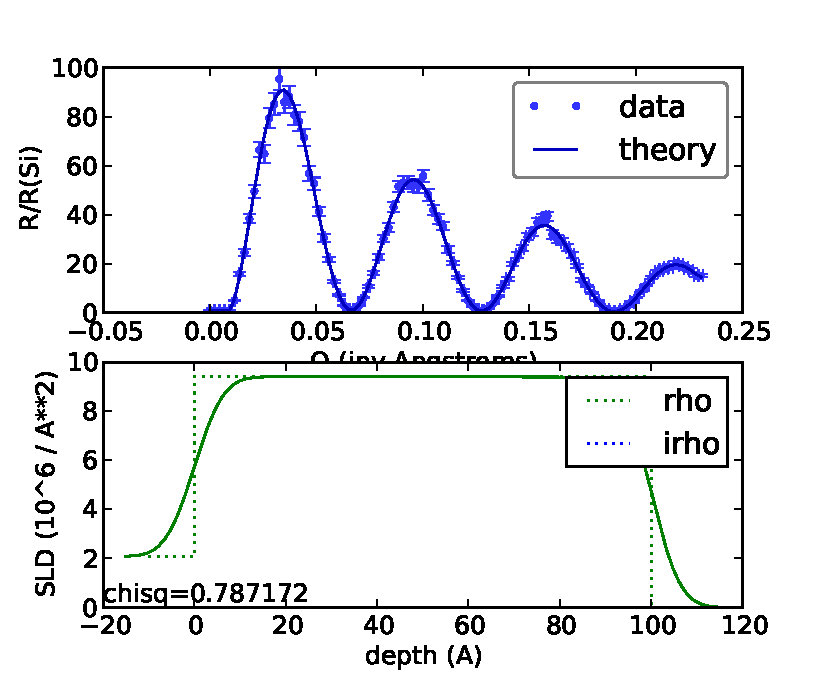
\includegraphics{a2ca71e2ff.pdf}

This model shows three layers (silicon, nickel, and air) as seen in the
solid green line (the step profile).  In addition we have a dashed green
line (the smoothed profile) which corresponds the effective reflectivity
profile, with the $\exp(-2 k_n k_{n+1} \sigma^2)$ interface factored in.

This model is defined in \code{nifilm.py}.

You can preview the model on the command line:

\begin{Verbatim}[commandchars=@\[\]]
@$ refl1d nifilm.py --preview
\end{Verbatim}

Lets examine the code down on a line by line basis to understand what is
going on.

The first step in any model is to load the names of the functions and
data that we are going to use.  These are defined in a module named
refl1d.names, and we import them all as follows:

\begin{Verbatim}[commandchars=@\[\]]
::
\end{Verbatim}
\begin{quote}

from refl1d.names import *
\end{quote}

This statement imports functions like SLD and Material for defining
materials, Parameter, Slab and Stack for defining materials,
NeutronProbe and XrayProbe for defining data, and Experiment and
FitProblem to tie everything together.

Note that `import *' is bad style for anything but simple scripts.  As
programs get larger, it is much less confusing to list the specific
functions that you need from a module rather than importing everything.

Next we define the materials that we are going to use in our sample.
silicon and air are common, so we don't need to define them.  We just
need to define nickel, which we do as follows:

\begin{Verbatim}[commandchars=@\[\]]
::
\end{Verbatim}
\begin{quote}

nickel = Material(`Ni')
\end{quote}

This defines a chemical formula, Ni, for which the program knows the
density in advance since it has densities for all elements.  By using
chemical composition, we can compute scattering length densities for
both X-ray and neutron beams from the same sample description.
Alternatively, we could take a more traditional approach and define
nickel as a specific SLD for our beam

\begin{Verbatim}[commandchars=@\[\]]
@PYGaE[@#nickel = SLD(rho=9.4)]
\end{Verbatim}

The `\#' character on the above line means that line is a comment, and
it won't be evaluated.

With our materials defined (silicon, nickel and air), we can combine
them into a sample. The substrate will be silicon with a 5 Å
1-$\sigma$ Si:Ni interface.  The nickel layer is 100 Å thick
with a 5 Å Ni:Air interface.  Air is on the surface.

\begin{Verbatim}[commandchars=@\[\]]
sample @PYGbe[=] silicon(@PYGaw[0],@PYGaw[5]) @PYGbe[@textbar[]] nickel(@PYGaw[100],@PYGaw[5]) @PYGbe[@textbar[]] air
\end{Verbatim}

Our sample definition is complete, so now we need to specify the
range of values we are going to view.  We will use the
\href{http://numpy.scipy.org/}{numpy} library, which extends python
with vector and matrix operations.  The \emph{linspace} function below
returns values from 0 to 5 in 100 steps for incident angles
from 0° to 5°.

\begin{Verbatim}[commandchars=@\[\]]
T @PYGbe[=] numpy@PYGbe[.]linspace(@PYGaw[0], @PYGaw[5], @PYGaw[100])
\end{Verbatim}

From the range of reflection angles, we can create a neutron probe. The probe
defines the wavelengths and angles which are used for the measurement as well
as their uncertainties.  From this the resolution of each point can be
calculated.  We use constants for angular divergence \code{dT=0.01}°,
wavelength \code{L=4.75} Å and wavelength dispersion \code{dL=0.0475} in this
example, but each angle and wavelength is independent.

\begin{Verbatim}[commandchars=@\[\]]
probe @PYGbe[=] NeutronProbe(T@PYGbe[=]T, dT@PYGbe[=]@PYGaw[0.01], L@PYGbe[=]@PYGaw[4.75], dL@PYGbe[=]@PYGaw[0.0475])
\end{Verbatim}

Combine the neutron probe with the sample stack to define an
experiment.  Using chemical formula and mass density, the same
sample can be simulated for both neutron and x-ray experiments.

\begin{Verbatim}[commandchars=@\[\]]
M @PYGbe[=] Experiment(probe@PYGbe[=]probe, sample@PYGbe[=]sample)
\end{Verbatim}

Generate a random data set with 5\% noise. While not necessary
to display a reflectivity curve, it is useful in showing how
the data set should look.

\begin{Verbatim}[commandchars=@\[\]]
M@PYGbe[.]simulate@_data(@PYGaw[5])
\end{Verbatim}

Combine a set of experiments into a fitting problem.  The problem
is used by refl1d for all operations on the model.

\begin{Verbatim}[commandchars=@\[\]]
problem @PYGbe[=] FitProblem(M)
\end{Verbatim}


\subsection{Choosing an instrument}
\label{examples/ex1/nifilm-tof:choosing-an-instrument}\label{examples/ex1/nifilm-tof::doc}
Let's modify the simulation to show how a 100 Å nickel film might
look if measured on the SNS Liquids reflectometer:

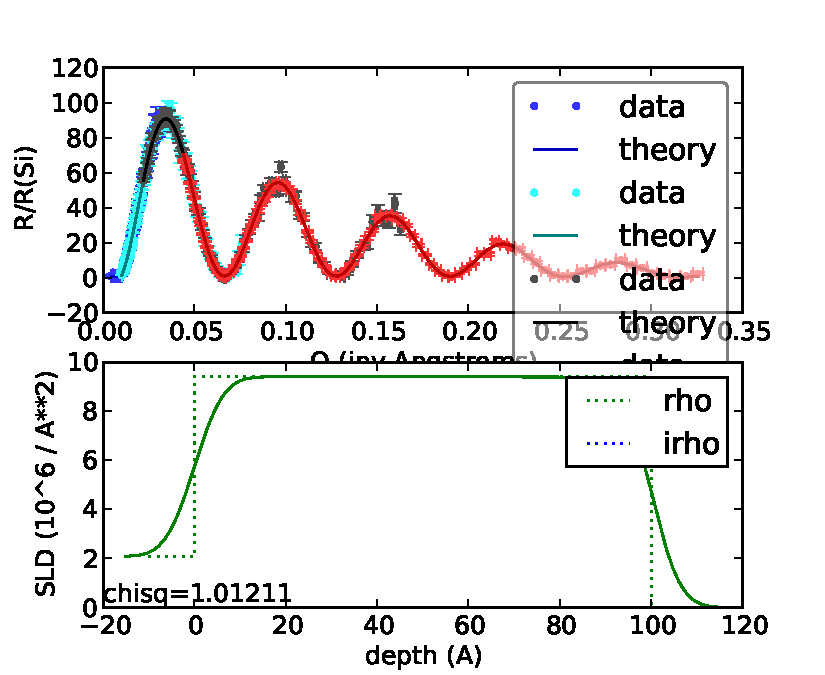
\includegraphics{9027665fb3.pdf}

This model is defined in \code{nifilm-tof.py}

The sample definition is the same:

\begin{Verbatim}[commandchars=@\[\]]
@PYGal[from] @PYGaW[refl1d.names] @PYGal[import] @PYGbe[*]

nickel @PYGbe[=] Material(@PYGaB[']@PYGaB[Ni]@PYGaB['])
sample @PYGbe[=] silicon(@PYGaw[0],@PYGaw[5]) @PYGbe[@textbar[]] nickel(@PYGaw[100],@PYGaw[5]) @PYGbe[@textbar[]] air
\end{Verbatim}

Instead of using a generic probe, we are using an instrument definition
to control the simulation.

\begin{Verbatim}[commandchars=@\[\]]
instrument @PYGbe[=] SNS@PYGbe[.]Liquids()
M @PYGbe[=] instrument@PYGbe[.]simulate(sample,
                        T@PYGbe[=]@PYGZlb[]@PYGaw[0.3],@PYGaw[0.7],@PYGaw[1.5],@PYGaw[3]@PYGZrb[],
                        slits@PYGbe[=]@PYGZlb[]@PYGaw[0.06], @PYGaw[0.14], @PYGaw[0.3], @PYGaw[0.6]@PYGZrb[],
                        uncertainty @PYGbe[=] @PYGaw[5],
                        )
\end{Verbatim}

The \emph{instrument} line tells us to use the geometry of the SNS Liquids
reflectometer, which includes information like the distance between the
sample and the slits and the wavelength range.  We then simulate measurements
of the sample for several different angles \emph{T} (degrees), each with its
own slit opening \emph{slits} (mm).  The simulated measurement duration is
such that the median relative error on the measurement $\Delta R/R$
will match \emph{uncertainty} (\%).  Because the intensity $I(\lambda)$ varies
so much for a time-of-flight measurement, the central points will be
measured with much better precision, and the end points will be measured
with lower precision.  See
{\hyperref[api/instrument:refl1d.instrument.Pulsed.simulate]{\code{Pulsed.simulate}}} for details
on all simulation parameters.

Finally, we bundle the simulated measurement as a fit problem which
is used by the rest of the program.

\begin{Verbatim}[commandchars=@\[\]]
problem @PYGbe[=] FitProblem(M)
\end{Verbatim}


\subsection{Attaching data}
\label{examples/ex1/nifilm-data:attaching-data}\label{examples/ex1/nifilm-data::doc}
Simulating data is great for seeing how models might look when measured
by a reflectometer, but mostly we are going to use the program to fit
measured data.  We saved the simulated data from above into files named
\code{nifilm-tof-1.dat}, \code{nifilm-tof-2.dat},
\code{nifilm-tof-3.dat} and \code{nifilm-tof-4.dat}.
We can load these datasets into a new model using
\code{nifilm-data.py}.

The sample and instrument definition is the same as before:

\begin{Verbatim}[commandchars=@\[\]]
@PYGal[from] @PYGaW[refl1d.names] @PYGal[import] @PYGbe[*]

nickel @PYGbe[=] Material(@PYGaB[']@PYGaB[Ni]@PYGaB['])
sample @PYGbe[=] silicon(@PYGaw[0],@PYGaw[5]) @PYGbe[@textbar[]] nickel(@PYGaw[100],@PYGaw[5]) @PYGbe[@textbar[]] air

instrument @PYGbe[=] SNS@PYGbe[.]Liquids()
\end{Verbatim}

In this case we are loading multiple data sets into the same
{\hyperref[api/probe:refl1d.probe.ProbeSet]{\code{ProbeSet}}} object.  If your
reduction program stitches together the data for you, then you can simply
use \code{probe=instrument.load('file')}.

\begin{Verbatim}[commandchars=@\[\]]
files @PYGbe[=] @PYGZlb[]@PYGaB[']@PYGaB[nifilm-tof-]@PYGbg[@%d]@PYGaB[.dat]@PYGaB[']@PYGbe[@%]d @PYGay[for] d @PYGav[in] @PYGaw[1],@PYGaw[2],@PYGaw[3],@PYGaw[4]@PYGZrb[]
probe @PYGbe[=] ProbeSet(instrument@PYGbe[.]load(f) @PYGay[for] f @PYGav[in] files)
\end{Verbatim}

The data and sample are combined into an
{\hyperref[api/experiment:refl1d.experiment.Experiment]{\code{Experiment}}},
which again is bundled as a
\code{FitProblem}
for the fitting program.

\begin{Verbatim}[commandchars=@\[\]]
M @PYGbe[=] Experiment(probe@PYGbe[=]probe, sample@PYGbe[=]sample)

problem @PYGbe[=] FitProblem(M)
\end{Verbatim}

The plot remains the same:

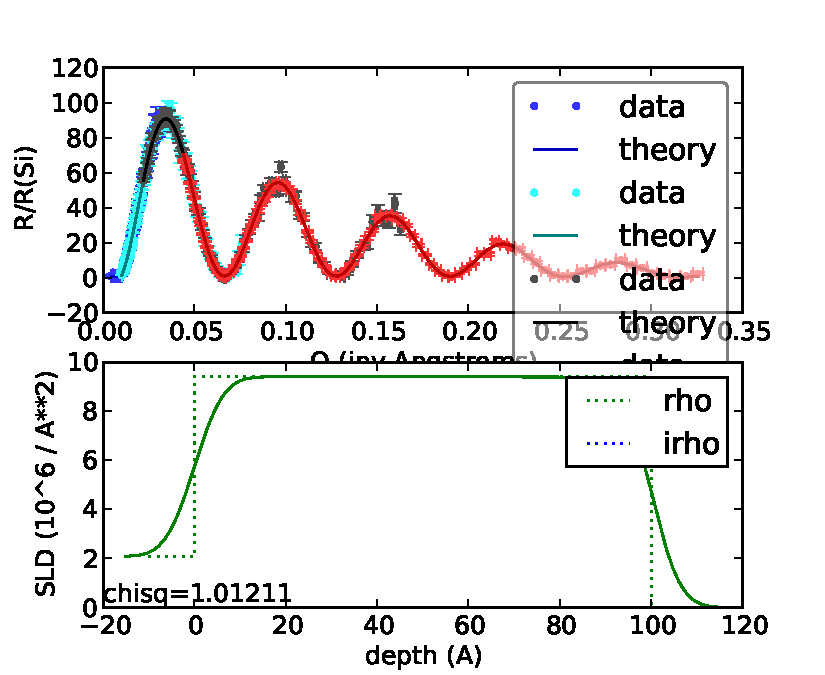
\includegraphics{564caae046.pdf}


\subsection{Performing a fit}
\label{examples/ex1/nifilm-fit:performing-a-fit}\label{examples/ex1/nifilm-fit::doc}
Now that we know how to define a sample and load data, we can learn how
to perform a fit on the data.  This is shown in
\code{nifilm-fit.py}:

We use the usual sample definition, except we set the thickness of the
nickel layer to 125 Å so that the model does not match the data:

\begin{Verbatim}[commandchars=@\[\]]
@PYGal[from] @PYGaW[refl1d.names] @PYGal[import] @PYGbe[*]

nickel @PYGbe[=] Material(@PYGaB[']@PYGaB[Ni]@PYGaB['])
sample @PYGbe[=] silicon(@PYGaw[0],@PYGaw[10]) @PYGbe[@textbar[]] nickel(@PYGaw[125],@PYGaw[10]) @PYGbe[@textbar[]] air
\end{Verbatim}

We are going to try to recover the original thickness by letting the
thickness value range by $125 \pm 50$ Å.  Since nickel is layer 1 in
the sample (counting starts at 0 in Python), we can access the layer
parameters using sample{[}1{]}.  The parameter we are accessing is the
thickness parameter, and we are setting it's fit range to $\pm 50$ Å.

\begin{Verbatim}[commandchars=@\[\]]
sample@PYGZlb[]@PYGaw[1]@PYGZrb[]@PYGbe[.]thickness@PYGbe[.]pm(@PYGaw[50])
\end{Verbatim}

We are also going to let the interfacial roughness between the layers vary.
The interface between two layers is defined by the width of the interface on
top of the layer below.  Here we are restricting the silicon:nickel interface
to the interval $[3,12]$ and the nickel:air interface to the range $[0,20]$:

\begin{Verbatim}[commandchars=@\[\]]
sample@PYGZlb[]@PYGaw[0]@PYGZrb[]@PYGbe[.]interface@PYGbe[.]range(@PYGaw[3],@PYGaw[12])
sample@PYGZlb[]@PYGaw[1]@PYGZrb[]@PYGbe[.]interface@PYGbe[.]range(@PYGaw[0],@PYGaw[20])
\end{Verbatim}

The data is loaded as before.

\begin{Verbatim}[commandchars=@\[\]]
instrument @PYGbe[=] SNS@PYGbe[.]Liquids()
files @PYGbe[=] @PYGZlb[]@PYGaB[']@PYGaB[nifilm-tof-]@PYGbg[@%d]@PYGaB[.dat]@PYGaB[']@PYGbe[@%]d @PYGay[for] d @PYGav[in] @PYGaw[1],@PYGaw[2],@PYGaw[3],@PYGaw[4]@PYGZrb[]
probe @PYGbe[=] ProbeSet(instrument@PYGbe[.]load(f) @PYGay[for] f @PYGav[in] files)

M @PYGbe[=] Experiment(probe@PYGbe[=]probe, sample@PYGbe[=]sample)

problem @PYGbe[=] FitProblem(M)
\end{Verbatim}

As you can see the new nickel thickness changes the theory curve
significantly:

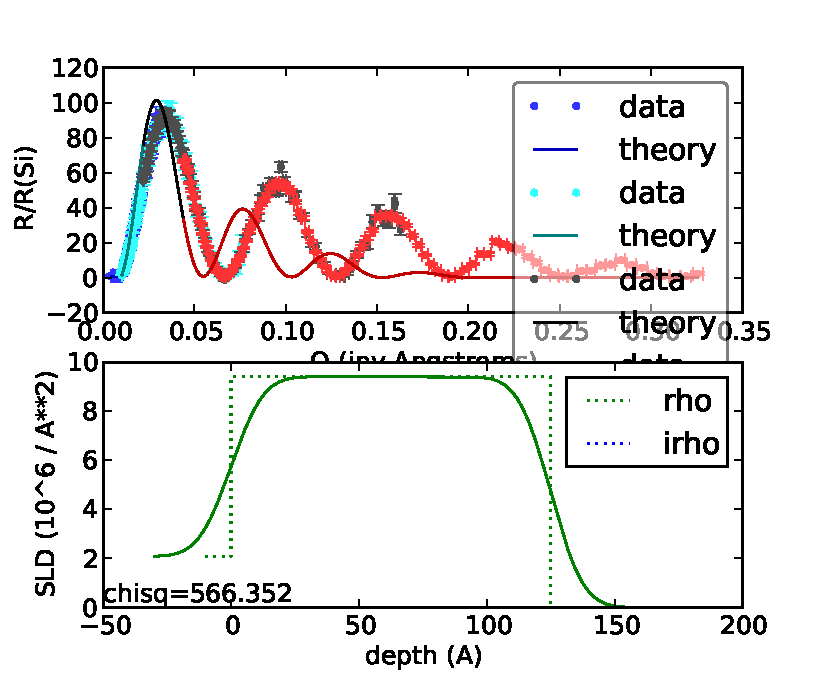
\includegraphics{f0e3f5eecb.pdf}

We can now load and run the fit:

\begin{Verbatim}[commandchars=@\[\]]
@PYGaE[@# refl1d nifilm-fit.py --fit=newton --steps=100 --store=T1]
\end{Verbatim}

The \code{-{-}fit=newton} option says to use the quasi-newton optimizer for
not more than 100 steps.  The \code{-{-}store=T1} option says to store the
initial model, the fit results and any monitoring information in the
directory T1.

Here is the resulting fit:

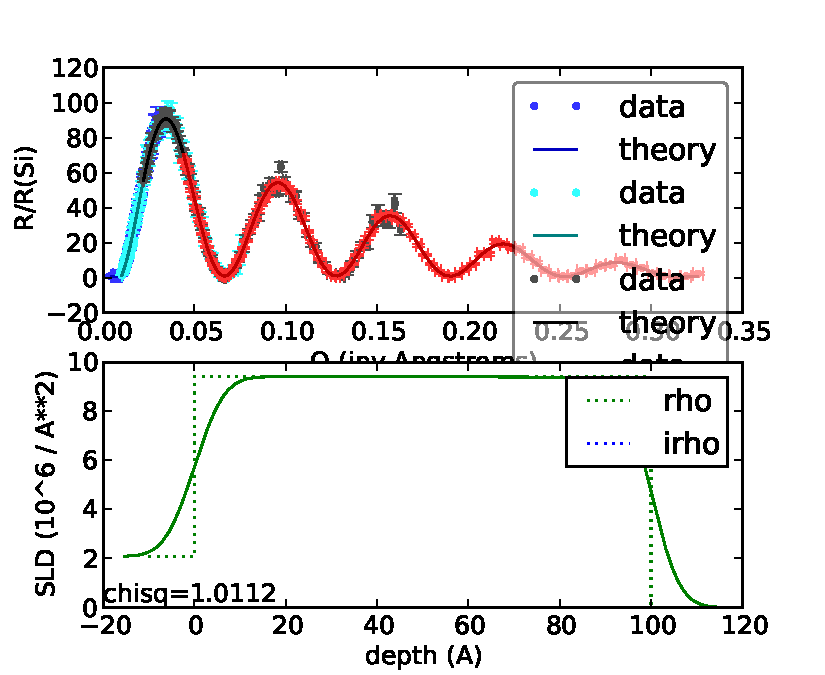
\includegraphics{fc43445452.pdf}

All is well: $\chi^2$ will be approximately 1 and the line goes nicely
through the data.


\subsection{Back reflectivity}
\label{examples/ex1/nifilm-back:back-reflectivity}\label{examples/ex1/nifilm-back::doc}
For samples measured with the incident beam through the substrate rather
than reflecting off the surface, we don't need to modify our sample, we
just need to tell the experiment that we are measuring back reflectivity.

We set up the example as before.

\begin{Verbatim}[commandchars=@\[\]]
@PYGal[from] @PYGaW[refl1d.names] @PYGal[import] @PYGbe[*]

nickel @PYGbe[=] Material(@PYGaB[']@PYGaB[Ni]@PYGaB['])
sample @PYGbe[=] silicon(@PYGaw[0],@PYGaw[25]) @PYGbe[@textbar[]] nickel(@PYGaw[100],@PYGaw[5]) @PYGbe[@textbar[]] air
T @PYGbe[=] numpy@PYGbe[.]linspace(@PYGaw[0], @PYGaw[5], @PYGaw[100])
\end{Verbatim}

Because we are measuring back reflectivity, we create a probe which has
back\_reflectivity = True.

\begin{Verbatim}[commandchars=@\[\]]
probe @PYGbe[=] NeutronProbe(T@PYGbe[=]T, dT@PYGbe[=]@PYGaw[0.01], L@PYGbe[=]@PYGaw[4.75], dL@PYGbe[=]@PYGaw[0.0475], back@_reflectivity@PYGbe[=]@PYGaA[True])
\end{Verbatim}

The remainder of the model definition is unchanged.

\begin{Verbatim}[commandchars=@\[\]]
M @PYGbe[=] Experiment(probe@PYGbe[=]probe, sample@PYGbe[=]sample)
M@PYGbe[.]simulate@_data(@PYGaw[5])
problem @PYGbe[=] FitProblem(M)
\end{Verbatim}


\section{Tethered Polymer}
\label{examples/polymer/readme::doc}\label{examples/polymer/readme:tethered-polymer}
Soft matter systems have more complex interfaces than slab layers with
gaussian roughness.

We will now model a data set for tethered deuterated polystyrene chains.
The chains start out at approximately 10 nm thick in dry conditions, and
swell to 14-18 nm thickness in toluene.  Two measurements were made:
\begin{itemize}
\item {} 
\code{10ndt001.refl} in deuterated toluene

\item {} 
\code{10nht001.refl}  in hydrogenated toluene

\end{itemize}

The chains are bound to the substrate by an initiator layer between the
substrate and brush chains. So the model needs a silicon layer, silicon
oxide layer, an initiator layer which is mostly hydrocarbon and
scattering length density should be between 0 and 1.5 depending on how
much solvent is in the layer. Then you have the swollen brush chains and
at the end bulk solvent. For these swelling measurements, the beam
penetrate the system from the silicon side and the bottom layer is
deuterated or hydrogenated toluene.


\subsection{Defining the film}
\label{examples/polymer/tethered:defining-the-film}\label{examples/polymer/tethered::doc}
We first need to define the materials

\begin{Verbatim}[commandchars=@\[\]]
@PYGal[from] @PYGaW[refl1d.names] @PYGal[import] @PYGbe[*]
@PYGal[from] @PYGaW[copy] @PYGal[import] copy

@PYGaE[@# === Materials ===]
SiOx @PYGbe[=] SLD(name@PYGbe[=]@PYGaB["]@PYGaB[SiOx]@PYGaB["],rho@PYGbe[=]@PYGaw[3.47])
D@_toluene @PYGbe[=] SLD(name@PYGbe[=]@PYGaB["]@PYGaB[D-toluene]@PYGaB["],rho@PYGbe[=]@PYGaw[5.66])
D@_initiator @PYGbe[=] SLD(name@PYGbe[=]@PYGaB["]@PYGaB[D-initiator]@PYGaB["],rho@PYGbe[=]@PYGaw[1.5])
D@_polystyrene @PYGbe[=] SLD(name@PYGbe[=]@PYGaB["]@PYGaB[D-PS]@PYGaB["],rho@PYGbe[=]@PYGaw[6.2])
H@_toluene @PYGbe[=] SLD(name@PYGbe[=]@PYGaB["]@PYGaB[H-toluene]@PYGaB["],rho@PYGbe[=]@PYGaw[0.94])
H@_initiator @PYGbe[=] SLD(name@PYGbe[=]@PYGaB["]@PYGaB[H-initiator]@PYGaB["],rho@PYGbe[=]@PYGaw[0])
\end{Verbatim}

In this case we are using the neutron scattering length density as is
standard practice in reflectivity experiments rather than the chemical
formula and mass density.  The {\hyperref[api/material:refl1d.material.SLD]{\code{SLD}}} class
allows us to name the material and define the real and imaginary components
of scattering length density $\rho$.  Note that we are using the imaginary
$\rho_i$ rather than the absorption coefficient $\mu = 2\lambda\rho_i$
since it removes the dependence on wavelength from the calculation of
the reflectivity.

For the tethered polymer we don't use a simple slab model, but instead
define a {\hyperref[api/polymer:refl1d.polymer.PolymerBrush]{\code{PolymerBrush}}}
layer, which understands that the system is compose of polymer plus
solvent, and that the polymer chains tail off like:
\begin{gather}
\begin{split}V(z) = \left\{
       \begin{array}{ll}
        V_o                        & \mbox{if } z <= z_o \\
        V_o (1 - ((z-z_o)/L)^2)^p  & \mbox{if } z_o < z < z_o + L \\
        0                          & \mbox{if } z >= z_o + L
        \end{array}
       \right.\end{split}\notag
\end{gather}
This volume profile combines with the scattering length density of the
polymer and the solvent to form an SLD profile:
\begin{gather}
\begin{split}\rho(z) = \rho_p V(z) + \rho_s (1 - V(z))\end{split}\notag
\end{gather}
The tethered polymer layer definition looks like

\begin{Verbatim}[commandchars=@\[\]]
@PYGaE[@# === Sample ===]
@PYGaE[@# Deuterated sample]
D@_brush @PYGbe[=] PolymerBrush(polymer@PYGbe[=]D@_polystyrene, solvent@PYGbe[=]D@_toluene,
                       base@_vf@PYGbe[=]@PYGaw[70], base@PYGbe[=]@PYGaw[120], length@PYGbe[=]@PYGaw[80], power@PYGbe[=]@PYGaw[2],
                       sigma@PYGbe[=]@PYGaw[10])
\end{Verbatim}

This layer can be combined with the remaining layers to form the
deuterated measurement sample

\begin{Verbatim}[commandchars=@\[\]]
D @PYGbe[=] (silicon(@PYGaw[0],@PYGaw[5]) @PYGbe[@textbar[]] SiOx(@PYGaw[100],@PYGaw[5]) @PYGbe[@textbar[]] D@_initiator(@PYGaw[100],@PYGaw[20]) @PYGbe[@textbar[]] D@_brush(@PYGaw[400],@PYGaw[0])
     @PYGbe[@textbar[]] D@_toluene)
\end{Verbatim}

The stack notation \code{material(thickness, interface) \textbar{} ...} is performing
a number of tasks for you.  One thing it is doing is wrapping materials
(which are objects that understand scattering length densities) into
slabs (which are objects that understand thickness and interface).  These
slabs are then gathered together into a stack:

\begin{Verbatim}[commandchars=@\[\]]
L@_silicon @PYGbe[=] Slab(material@PYGbe[=]silicon, thickness@PYGbe[=]@PYGaw[0], interface@PYGbe[=]@PYGaw[5])
L@_SiOx @PYGbe[=] Slab(material@PYGbe[=]SiOx, thickness@PYGbe[=]@PYGaw[100], interface@PYGbe[=]@PYGaw[5])
L@_D@_initiator @PYGbe[=] Slab(material@PYGbe[=]D@_initiator, thickness@PYGbe[=]@PYGaw[100], interface@PYGbe[=]@PYGaw[20])
L@_D@_brush @PYGbe[=] copy(D@_brush)
L@_D@_brush@PYGbe[.]thickness @PYGbe[=] Parameter@PYGbe[.]default(@PYGaw[400],name@PYGbe[=]D@_brush@PYGbe[.]name@PYGbe[+]@PYGaB["]@PYGaB[ thickness]@PYGaB["])
L@_D@_brush@PYGbe[.]interface @PYGbe[=] Parameter@PYGbe[.]default(@PYGaw[0],name@PYGbe[=]D@_brush@PYGbe[.]name@PYGbe[+]@PYGaB["]@PYGaB[ interface]@PYGaB["])
L@_D@_toluene @PYGbe[=] Slab(material@PYGbe[=]D@_toluene)
D @PYGbe[=] Stack(@PYGZlb[]L@_silicon, L@_SiOx, L@_D@_initiator, L@_D@_brush, L@_D@_toluene@PYGZrb[])
\end{Verbatim}

The undeuterated sample is similar to the deuterated sample. We start
by copying the polymer brush layer so that parameters such as \emph{length},
\emph{power}, etc. will be shared between the two systems, but we replace the
deuterated toluene solvent with undeuterated toluene.  We then use
this \emph{H\_brush} to define a new stack with undeuterated tolune

\begin{Verbatim}[commandchars=@\[\]]
@PYGaE[@# Undeuterated sample is a copy of the deuterated sample]
H@_brush @PYGbe[=] copy(D@_brush)       @PYGaE[@# Share tethered polymer parameters...]
H@_brush@PYGbe[.]solvent @PYGbe[=] H@_toluene   @PYGaE[@# ... but use different solvent]
H @PYGbe[=] silicon @PYGbe[@textbar[]] SiOx @PYGbe[@textbar[]] H@_initiator @PYGbe[@textbar[]] H@_brush @PYGbe[@textbar[]] H@_toluene
\end{Verbatim}

We want to share thickness and interface between the two systems
as well, so we write a loop to go through the layers of \emph{D} and
copy the thickness and interface parameters to \emph{H}

\begin{Verbatim}[commandchars=@\[\]]
@PYGay[for] i,@_ @PYGav[in] @PYGaY[enumerate](D):
    H@PYGZlb[]i@PYGZrb[]@PYGbe[.]thickness @PYGbe[=] D@PYGZlb[]i@PYGZrb[]@PYGbe[.]thickness
    H@PYGZlb[]i@PYGZrb[]@PYGbe[.]interface @PYGbe[=] D@PYGZlb[]i@PYGZrb[]@PYGbe[.]interface
\end{Verbatim}

What is happening internally is that for each layer in the stack we are
copying the parameter for the thickness from the deuterated sample
slab to the thickness slot in the undeuterated sample slab.  Similarly
for interface.  When the refinement engine sets a new value for a
thickness parameter and asks the two models to evaluate $\chi^2$, both
models will see the same thickness parameter value.


\subsection{Setting fit ranges}
\label{examples/polymer/tethered:setting-fit-ranges}
With both samples defined, we next specify the ranges on the fitted
parameters

\begin{Verbatim}[commandchars=@\[\]]
@PYGaE[@# === Fit parameters ===]
@PYGay[for] i @PYGav[in] @PYGaw[0], @PYGaw[1], @PYGaw[2]:
    D@PYGZlb[]i@PYGZrb[]@PYGbe[.]interface@PYGbe[.]range(@PYGaw[0],@PYGaw[100])
D@PYGZlb[]@PYGaw[1]@PYGZrb[]@PYGbe[.]thickness@PYGbe[.]range(@PYGaw[0],@PYGaw[200])
D@PYGZlb[]@PYGaw[2]@PYGZrb[]@PYGbe[.]thickness@PYGbe[.]range(@PYGaw[0],@PYGaw[200])
D@_polystyrene@PYGbe[.]rho@PYGbe[.]range(@PYGaw[6.2],@PYGaw[6.5])
SiOx@PYGbe[.]rho@PYGbe[.]range(@PYGaw[2.07],@PYGaw[4.16]) @PYGaE[@# Si to SiO2]
D@_toluene@PYGbe[.]rho@PYGbe[.]pmp(@PYGaw[5])
D@_initiator@PYGbe[.]rho@PYGbe[.]range(@PYGaw[0],@PYGaw[1.5])
D@_brush@PYGbe[.]base@_vf@PYGbe[.]range(@PYGaw[50],@PYGaw[80])
D@_brush@PYGbe[.]base@PYGbe[.]range(@PYGaw[0],@PYGaw[200])
D@_brush@PYGbe[.]length@PYGbe[.]range(@PYGaw[0],@PYGaw[500])
D@_brush@PYGbe[.]power@PYGbe[.]range(@PYGaw[0],@PYGaw[5])
D@_brush@PYGbe[.]sigma@PYGbe[.]range(@PYGaw[0],@PYGaw[20])

@PYGaE[@# Undeuterated system adds two extra parameters]
H@_toluene@PYGbe[.]rho@PYGbe[.]pmp(@PYGaw[5])
H@_initiator@PYGbe[.]rho@PYGbe[.]range(@PYGbe[-]@PYGaw[0.5],@PYGaw[0.5])
\end{Verbatim}

Notice that in some cases we are using layer number to reference the
parameter, such as \code{D{[}1{]}.thickness} whereas in other cases we are using
variables directly, such as \code{D\_toluene.rho}.  Determining which to
use requires an understanding of the underlying stack model.  In this
case, the thickness is associated with the SiOx slab thickness, but
we never formed a variable to contain \code{Slab(material=SiOx)}, so we
have to reference it via the stack.   We did however create a variable
to contain \code{Material(name="D\_toluene")} so we can access its parameters
directly.  Also, notice that we only need to set one of \code{D{[}1{]}.thickness}
and \code{H{[}1{]}.thickness} since they are the same underlying parameter.


\subsection{Attaching data}
\label{examples/polymer/tethered:attaching-data}
Next we associate the reflectivity curves with the samples:

\begin{Verbatim}[commandchars=@\[\]]
@PYGaE[@# === Data files ===]
instrument @PYGbe[=] NCNR@PYGbe[.]NG7(Qlo@PYGbe[=]@PYGaw[0.005], slits@_at@_Qlo@PYGbe[=]@PYGaw[0.075])
D@_probe @PYGbe[=] instrument@PYGbe[.]load(@PYGaB[']@PYGaB[10ndt001.refl]@PYGaB['], back@_reflectivity@PYGbe[=]@PYGaA[True])
H@_probe @PYGbe[=] instrument@PYGbe[.]load(@PYGaB[']@PYGaB[10nht001.refl]@PYGaB['], back@_reflectivity@PYGbe[=]@PYGaA[True])
\end{Verbatim}

We set \code{back\_reflectivity=True} because we are coming in through the
substrate.  The reflectometry calculator will automatically reverse
the stack and adjust the effective incident angle to account for the
refraction when the beam enters the side of the substrate.  Ideally
you will have measured the incident beam intensity through the substrate
as well so that substrate absorption effects are corrected for in your
data reduction steps, but if not, you can set an estimate for
\code{back\_absorption} when you load the file.  Like \code{intensity} you can
set a range on the value and adjust it during refinement.

Finally, we define the fitting problem from the probes and samples.
The dz parameter controls the size of the profiles steps when generating
the tethered polymer interface.  The dA parameter allows these steps
to be joined together into larger slabs, with each slab having
$(\rho_{\text max} - \rho_{\text min}) w < \Delta A$.

\begin{Verbatim}[commandchars=@\[\]]
@PYGaE[@# === Problem definition ===]
D@_model @PYGbe[=] Experiment(sample@PYGbe[=]D, probe@PYGbe[=]D@_probe, dz@PYGbe[=]@PYGaw[0.5], dA@PYGbe[=]@PYGaw[1])
H@_model @PYGbe[=] Experiment(sample@PYGbe[=]H, probe@PYGbe[=]H@_probe, dz@PYGbe[=]@PYGaw[0.5], dA@PYGbe[=]@PYGaw[1])
models @PYGbe[=] H@_model, D@_model
\end{Verbatim}

This is a multifit problem where both models contribute to the goodness
of fit measure $\chi^2$.  Since no weight vector was defined the fits
have equal weight.

\begin{Verbatim}[commandchars=@\[\]]
problem @PYGbe[=] MultiFitProblem(models@PYGbe[=]models)
problem@PYGbe[.]name @PYGbe[=] @PYGaB["]@PYGaB[tethered]@PYGaB["]
\end{Verbatim}

The polymer brush model is a smooth profile function, which is evaluated
by slicing it into thin slabs, then joining together similar slabs to
improve evaluation time.  The \code{dz=0.5} parameter tells us that we
should slice the brush into 0.5 Å steps.  The \code{dA=1} parameter
says we should join together thin slabs while the scattering density
uncertainty in the joined slabs $\Delta A < 1$, where
$\Delta A = (\max\rho - \min\rho)(\max z - \min z)$.  Similarly for
the absorption cross section $\rho_i$ and the effective magnetic cross
section $\rho_M \cos(\theta_M)$.  If \code{dA=None} (the default) then no
profile contraction occurs.

The resulting model looks like:

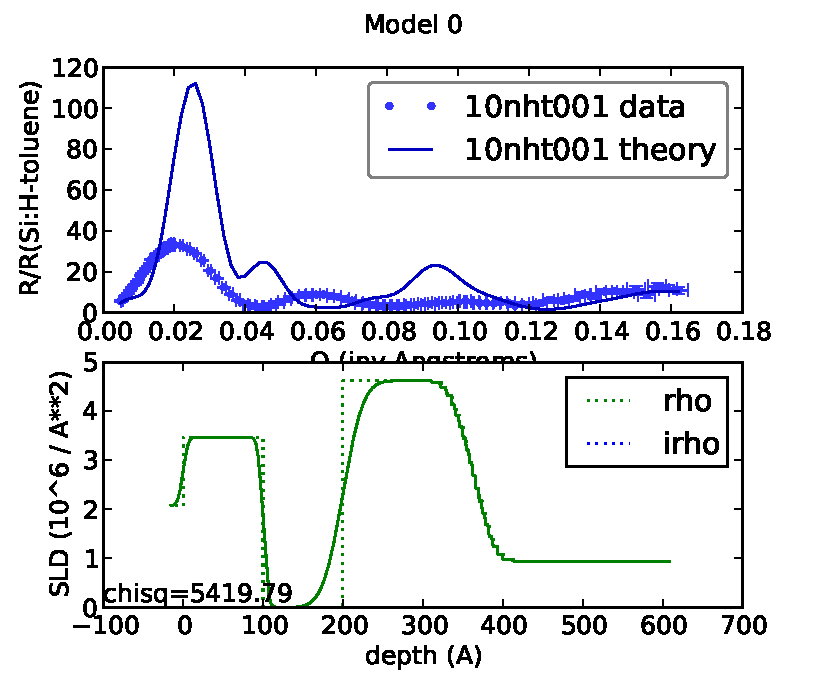
\includegraphics{0808430085_00.pdf}

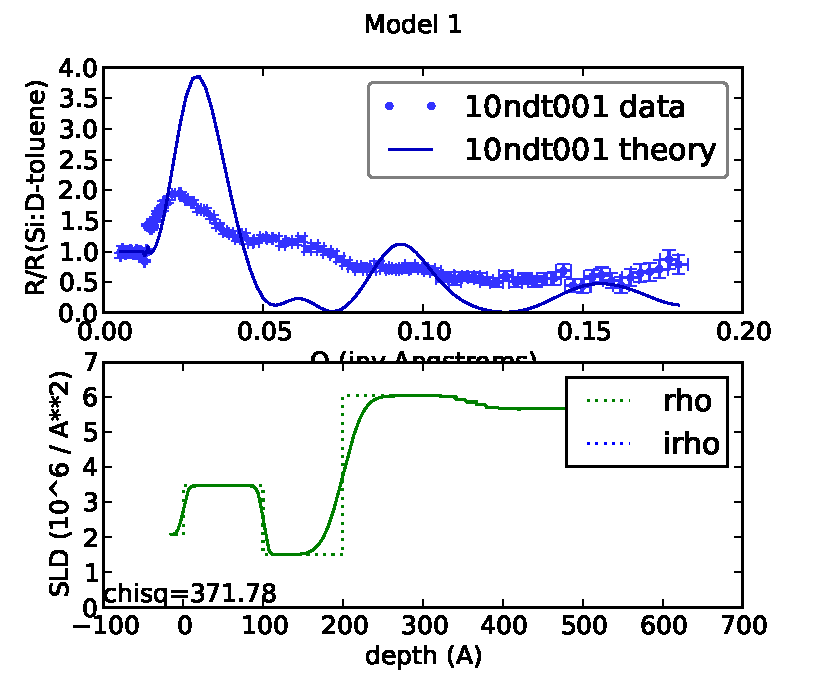
\includegraphics{0808430085_01.pdf}

This complete model script is defined in
\code{tethered.py}:

\begin{Verbatim}[commandchars=@\[\]]
@PYGal[from] @PYGaW[refl1d.names] @PYGal[import] @PYGbe[*]
@PYGal[from] @PYGaW[copy] @PYGal[import] copy

@PYGaE[@# === Materials ===]
SiOx @PYGbe[=] SLD(name@PYGbe[=]@PYGaB["]@PYGaB[SiOx]@PYGaB["],rho@PYGbe[=]@PYGaw[3.47])
D@_toluene @PYGbe[=] SLD(name@PYGbe[=]@PYGaB["]@PYGaB[D-toluene]@PYGaB["],rho@PYGbe[=]@PYGaw[5.66])
D@_initiator @PYGbe[=] SLD(name@PYGbe[=]@PYGaB["]@PYGaB[D-initiator]@PYGaB["],rho@PYGbe[=]@PYGaw[1.5])
D@_polystyrene @PYGbe[=] SLD(name@PYGbe[=]@PYGaB["]@PYGaB[D-PS]@PYGaB["],rho@PYGbe[=]@PYGaw[6.2])
H@_toluene @PYGbe[=] SLD(name@PYGbe[=]@PYGaB["]@PYGaB[H-toluene]@PYGaB["],rho@PYGbe[=]@PYGaw[0.94])
H@_initiator @PYGbe[=] SLD(name@PYGbe[=]@PYGaB["]@PYGaB[H-initiator]@PYGaB["],rho@PYGbe[=]@PYGaw[0])

@PYGaE[@# === Sample ===]
@PYGaE[@# Deuterated sample]
D@_brush @PYGbe[=] PolymerBrush(polymer@PYGbe[=]D@_polystyrene, solvent@PYGbe[=]D@_toluene,
                       base@_vf@PYGbe[=]@PYGaw[70], base@PYGbe[=]@PYGaw[120], length@PYGbe[=]@PYGaw[80], power@PYGbe[=]@PYGaw[2],
                       sigma@PYGbe[=]@PYGaw[10])

D @PYGbe[=] (silicon(@PYGaw[0],@PYGaw[5]) @PYGbe[@textbar[]] SiOx(@PYGaw[100],@PYGaw[5]) @PYGbe[@textbar[]] D@_initiator(@PYGaw[100],@PYGaw[20]) @PYGbe[@textbar[]] D@_brush(@PYGaw[400],@PYGaw[0])
     @PYGbe[@textbar[]] D@_toluene)

@PYGaE[@# Undeuterated sample is a copy of the deuterated sample]
H@_brush @PYGbe[=] copy(D@_brush)       @PYGaE[@# Share tethered polymer parameters...]
H@_brush@PYGbe[.]solvent @PYGbe[=] H@_toluene   @PYGaE[@# ... but use different solvent]
H @PYGbe[=] silicon @PYGbe[@textbar[]] SiOx @PYGbe[@textbar[]] H@_initiator @PYGbe[@textbar[]] H@_brush @PYGbe[@textbar[]] H@_toluene

@PYGay[for] i,@_ @PYGav[in] @PYGaY[enumerate](D):
    H@PYGZlb[]i@PYGZrb[]@PYGbe[.]thickness @PYGbe[=] D@PYGZlb[]i@PYGZrb[]@PYGbe[.]thickness
    H@PYGZlb[]i@PYGZrb[]@PYGbe[.]interface @PYGbe[=] D@PYGZlb[]i@PYGZrb[]@PYGbe[.]interface

@PYGaE[@# === Fit parameters ===]
@PYGay[for] i @PYGav[in] @PYGaw[0], @PYGaw[1], @PYGaw[2]:
    D@PYGZlb[]i@PYGZrb[]@PYGbe[.]interface@PYGbe[.]range(@PYGaw[0],@PYGaw[100])
D@PYGZlb[]@PYGaw[1]@PYGZrb[]@PYGbe[.]thickness@PYGbe[.]range(@PYGaw[0],@PYGaw[200])
D@PYGZlb[]@PYGaw[2]@PYGZrb[]@PYGbe[.]thickness@PYGbe[.]range(@PYGaw[0],@PYGaw[200])
D@_polystyrene@PYGbe[.]rho@PYGbe[.]range(@PYGaw[6.2],@PYGaw[6.5])
SiOx@PYGbe[.]rho@PYGbe[.]range(@PYGaw[2.07],@PYGaw[4.16]) @PYGaE[@# Si to SiO2]
D@_toluene@PYGbe[.]rho@PYGbe[.]pmp(@PYGaw[5])
D@_initiator@PYGbe[.]rho@PYGbe[.]range(@PYGaw[0],@PYGaw[1.5])
D@_brush@PYGbe[.]base@_vf@PYGbe[.]range(@PYGaw[50],@PYGaw[80])
D@_brush@PYGbe[.]base@PYGbe[.]range(@PYGaw[0],@PYGaw[200])
D@_brush@PYGbe[.]length@PYGbe[.]range(@PYGaw[0],@PYGaw[500])
D@_brush@PYGbe[.]power@PYGbe[.]range(@PYGaw[0],@PYGaw[5])
D@_brush@PYGbe[.]sigma@PYGbe[.]range(@PYGaw[0],@PYGaw[20])

@PYGaE[@# Undeuterated system adds two extra parameters]
H@_toluene@PYGbe[.]rho@PYGbe[.]pmp(@PYGaw[5])
H@_initiator@PYGbe[.]rho@PYGbe[.]range(@PYGbe[-]@PYGaw[0.5],@PYGaw[0.5])

@PYGaE[@# === Data files ===]
instrument @PYGbe[=] NCNR@PYGbe[.]NG7(Qlo@PYGbe[=]@PYGaw[0.005], slits@_at@_Qlo@PYGbe[=]@PYGaw[0.075])
D@_probe @PYGbe[=] instrument@PYGbe[.]load(@PYGaB[']@PYGaB[10ndt001.refl]@PYGaB['], back@_reflectivity@PYGbe[=]@PYGaA[True])
H@_probe @PYGbe[=] instrument@PYGbe[.]load(@PYGaB[']@PYGaB[10nht001.refl]@PYGaB['], back@_reflectivity@PYGbe[=]@PYGaA[True])

@PYGaE[@# === Problem definition ===]
D@_model @PYGbe[=] Experiment(sample@PYGbe[=]D, probe@PYGbe[=]D@_probe, dz@PYGbe[=]@PYGaw[0.5], dA@PYGbe[=]@PYGaw[1])
H@_model @PYGbe[=] Experiment(sample@PYGbe[=]H, probe@PYGbe[=]H@_probe, dz@PYGbe[=]@PYGaw[0.5], dA@PYGbe[=]@PYGaw[1])
models @PYGbe[=] H@_model, D@_model

problem @PYGbe[=] MultiFitProblem(models@PYGbe[=]models)
problem@PYGbe[.]name @PYGbe[=] @PYGaB["]@PYGaB[tethered]@PYGaB["]
\end{Verbatim}

The model can be fit using the parallel tempering optimizer:

\begin{Verbatim}[commandchars=@\[\]]
@$ refl1d tethered.py --fit=pt --store=T1
\end{Verbatim}


\section{Composite sample}
\label{examples/mixed/readme:composite-sample}\label{examples/mixed/readme::doc}
There are conditions wherein the sample you measure is not ideal.  For
example, a polymer brush may have enough density in some domains that
the brushes are standing upright, but in other domains the brushes
lie flat.


\subsection{Channel measurement}
\label{examples/mixed/mixed:channel-measurement}\label{examples/mixed/mixed::doc}
In this example we will look at a nickel grating on a silicon substrate
using specular reflectivity. When the spacing within the grating is
sufficiently large, this can be modeled to first order as the incoherent sum
of the reflectivity on the plateau and the reflectivity on the valley floor.
By adjusting the weight of two reflectivities, we should be able to
determine the ratio of plateau width to valley width.

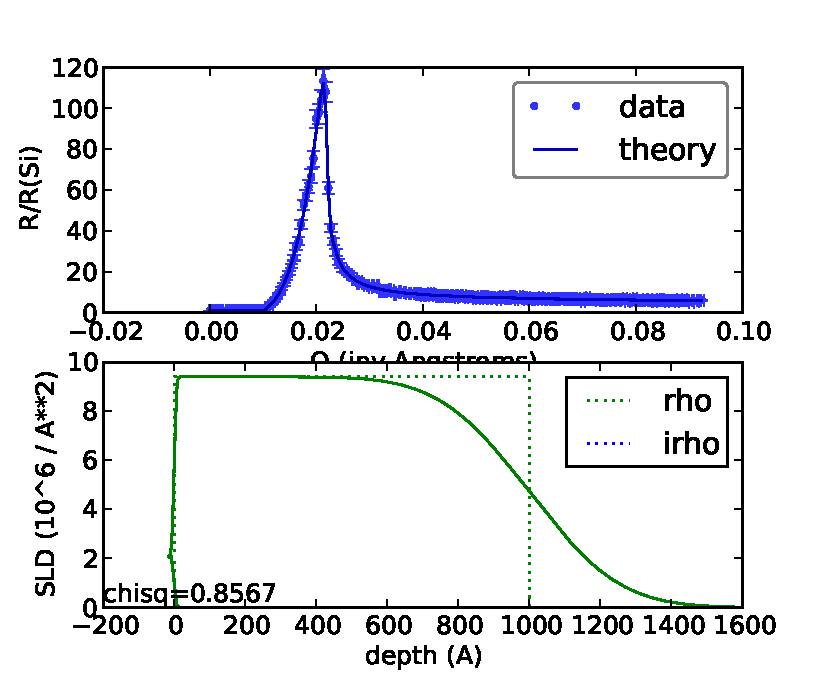
\includegraphics{059ce42618.pdf}

Since silicon and air are defined, the only material we need to
define is nickel.

\begin{Verbatim}[commandchars=@\[\]]
@PYGal[from] @PYGaW[refl1d.names] @PYGal[import] @PYGbe[*]
nickel @PYGbe[=] Material(@PYGaB[']@PYGaB[Ni]@PYGaB['])
\end{Verbatim}

We need two separate models, one with 1000 Å nickel and one without.

\begin{Verbatim}[commandchars=@\[\]]
plateau @PYGbe[=] silicon(@PYGaw[0],@PYGaw[5]) @PYGbe[@textbar[]] nickel(@PYGaw[1000],@PYGaw[200]) @PYGbe[@textbar[]] air
valley @PYGbe[=] silicon(@PYGaw[0],@PYGaw[5]) @PYGbe[@textbar[]] air
\end{Verbatim}

We need only one probe for simulation.  The reflectivity measured at
the detector will be a mixture of those neutrons which reflect off
the plateau and those that reflect off the valley.

\begin{Verbatim}[commandchars=@\[\]]
T @PYGbe[=] numpy@PYGbe[.]linspace(@PYGaw[0], @PYGaw[2], @PYGaw[200])
probe @PYGbe[=] NeutronProbe(T@PYGbe[=]T, dT@PYGbe[=]@PYGaw[0.01], L@PYGbe[=]@PYGaw[4.75], dL@PYGbe[=]@PYGaw[0.0475])
\end{Verbatim}

We are going to start with a 1:1 ratio of plateau to valley and create
a simulated data set.

\begin{Verbatim}[commandchars=@\[\]]
M @PYGbe[=] MixedExperiment(samples@PYGbe[=]@PYGZlb[]plateau,valley@PYGZrb[], probe@PYGbe[=]probe, ratio@PYGbe[=]@PYGZlb[]@PYGaw[1],@PYGaw[1]@PYGZrb[])
M@PYGbe[.]simulate@_data(@PYGaw[5])
\end{Verbatim}

We will assume the silicon interface is the same for the valley as the
plateau, which depending on the how the sample is constructed, may or
may not be realistic.

\begin{Verbatim}[commandchars=@\[\]]
valley@PYGZlb[]@PYGaw[0]@PYGZrb[]@PYGbe[.]interface @PYGbe[=] plateau@PYGZlb[]@PYGaw[0]@PYGZrb[]@PYGbe[.]interface
\end{Verbatim}

We will want to fit the thicknesses and interfaces as usual.

\begin{Verbatim}[commandchars=@\[\]]
plateau@PYGZlb[]@PYGaw[0]@PYGZrb[]@PYGbe[.]interface@PYGbe[.]range(@PYGaw[0],@PYGaw[200])
plateau@PYGZlb[]@PYGaw[1]@PYGZrb[]@PYGbe[.]interface@PYGbe[.]range(@PYGaw[0],@PYGaw[200])
plateau@PYGZlb[]@PYGaw[1]@PYGZrb[]@PYGbe[.]thickness@PYGbe[.]range(@PYGaw[200],@PYGaw[1800])
\end{Verbatim}

The ratio between the valley and the plateau can also be fit, either
by fixing size of the plateau and fitting the size of the valley or
fixing the size of the valley and fitting the size of the plateau.  We
will hold the plateau fixed.

\begin{Verbatim}[commandchars=@\[\]]
M@PYGbe[.]ratio@PYGZlb[]@PYGaw[1]@PYGZrb[]@PYGbe[.]range(@PYGaw[0],@PYGaw[5])
\end{Verbatim}

Note that we could include a second order effect by including a
hillside term with the same height as the plateau but using a
50:50 mixture of air and nickel.  In this case we would have three
entries in the ratio.

We wrap this as a fit problem as usual.

\begin{Verbatim}[commandchars=@\[\]]
problem @PYGbe[=] FitProblem(M)
\end{Verbatim}

This complete model script is defined in
\code{mixed.py}:

\begin{Verbatim}[commandchars=@\[\]]
@PYGal[from] @PYGaW[refl1d.names] @PYGal[import] @PYGbe[*]
nickel @PYGbe[=] Material(@PYGaB[']@PYGaB[Ni]@PYGaB['])

plateau @PYGbe[=] silicon(@PYGaw[0],@PYGaw[5]) @PYGbe[@textbar[]] nickel(@PYGaw[1000],@PYGaw[200]) @PYGbe[@textbar[]] air
valley @PYGbe[=] silicon(@PYGaw[0],@PYGaw[5]) @PYGbe[@textbar[]] air

T @PYGbe[=] numpy@PYGbe[.]linspace(@PYGaw[0], @PYGaw[2], @PYGaw[200])
probe @PYGbe[=] NeutronProbe(T@PYGbe[=]T, dT@PYGbe[=]@PYGaw[0.01], L@PYGbe[=]@PYGaw[4.75], dL@PYGbe[=]@PYGaw[0.0475])

M @PYGbe[=] MixedExperiment(samples@PYGbe[=]@PYGZlb[]plateau,valley@PYGZrb[], probe@PYGbe[=]probe, ratio@PYGbe[=]@PYGZlb[]@PYGaw[1],@PYGaw[1]@PYGZrb[])
M@PYGbe[.]simulate@_data(@PYGaw[5])

valley@PYGZlb[]@PYGaw[0]@PYGZrb[]@PYGbe[.]interface @PYGbe[=] plateau@PYGZlb[]@PYGaw[0]@PYGZrb[]@PYGbe[.]interface

plateau@PYGZlb[]@PYGaw[0]@PYGZrb[]@PYGbe[.]interface@PYGbe[.]range(@PYGaw[0],@PYGaw[200])
plateau@PYGZlb[]@PYGaw[1]@PYGZrb[]@PYGbe[.]interface@PYGbe[.]range(@PYGaw[0],@PYGaw[200])
plateau@PYGZlb[]@PYGaw[1]@PYGZrb[]@PYGbe[.]thickness@PYGbe[.]range(@PYGaw[200],@PYGaw[1800])

M@PYGbe[.]ratio@PYGZlb[]@PYGaw[1]@PYGZrb[]@PYGbe[.]range(@PYGaw[0],@PYGaw[5])

problem @PYGbe[=] FitProblem(M)
\end{Verbatim}

We can test how well the fitter can recover the original model
by running refl1d with --random:

\begin{Verbatim}[commandchars=@\[\]]
@$ refl1d mixed.py --random --store=T1
\end{Verbatim}


\section{Superlattice Models}
\label{examples/superlattice/readme::doc}\label{examples/superlattice/readme:superlattice-models}
Any structure can be turned into a superlattice using a {\hyperref[api/model:refl1d.model.Repeat]{\code{refl1d.model.Repeat}}}.

Simply form a stack as usual, then use that stack within another stack, with a
repeat modifier.


\subsection{Hard material structures}
\label{examples/superlattice/NiTi:hard-material-structures}\label{examples/superlattice/NiTi::doc}
Here is an example of a multilayer system in the literature:
\begin{quote}

Singh, S., Basu, S., Bhatt, P., Poswal, A.K.,
Phys. Rev. B, 79, 195435 (2009)
\end{quote}

In this paper, the authors are interested in the interdiffusion properties
of Ni into Ti through x-ray and neutron reflectivity measurements. The
question of alloying at metal-metal interfaces at elevated temperatures is
critically important for device fabrication and reliability.

The model is defined in \code{NiTi.py}.

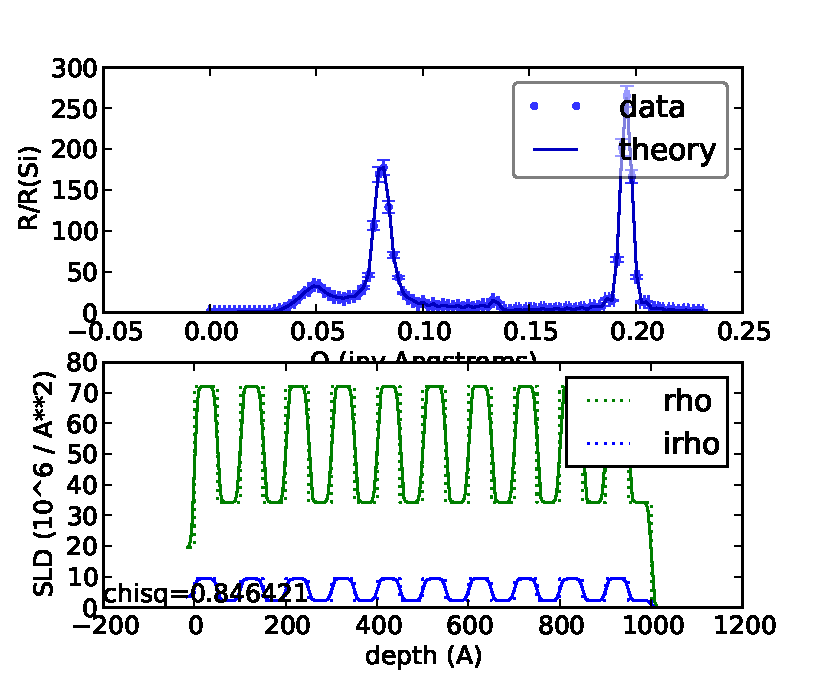
\includegraphics{e1eb8621b4.pdf}

First define the materials we will use

\begin{Verbatim}[commandchars=@\[\]]
@PYGal[from] @PYGaW[refl1d.names] @PYGal[import] @PYGbe[*]

nickel @PYGbe[=] Material(@PYGaB[']@PYGaB[Ni]@PYGaB['])
titanium @PYGbe[=] Material(@PYGaB[']@PYGaB[Ti]@PYGaB['])
\end{Verbatim}

Next we will compose nickel and titanium into a bilayer and use that
bilayer to define a stack with 10 repeats.

\begin{Verbatim}[commandchars=@\[\]]
@PYGaE[@# Superlattice description]
bilayer @PYGbe[=] nickel(@PYGaw[50],@PYGaw[5]) @PYGbe[@textbar[]] titanium(@PYGaw[50],@PYGaw[5])
sample @PYGbe[=] silicon(@PYGaw[0],@PYGaw[5]) @PYGbe[@textbar[]] bilayer@PYGbe[*]@PYGaw[10] @PYGbe[@textbar[]] air
\end{Verbatim}

We allow the thickness to vary by +/- 100\%

\begin{Verbatim}[commandchars=@\[\]]
@PYGaE[@# Fitting parameters]
bilayer@PYGZlb[]@PYGaw[0]@PYGZrb[]@PYGbe[.]thickness@PYGbe[.]pmp(@PYGaw[100])
bilayer@PYGZlb[]@PYGaw[1]@PYGZrb[]@PYGbe[.]thickness@PYGbe[.]pmp(@PYGaw[100])
\end{Verbatim}

The interfaces vary between 0 and 30 Å. The interface between repeats is
defined by the interface at the top of the repeating stack, which in this case
is the Ti interface.  The interface between the superlattice and the next
layer is an independent parameter, whose value defaults to the same initial
value as the interface between the repeats.

\begin{Verbatim}[commandchars=@\[\]]
bilayer@PYGZlb[]@PYGaw[0]@PYGZrb[]@PYGbe[.]interface@PYGbe[.]range(@PYGaw[0],@PYGaw[30])
bilayer@PYGZlb[]@PYGaw[1]@PYGZrb[]@PYGbe[.]interface@PYGbe[.]range(@PYGaw[0],@PYGaw[30])
sample@PYGZlb[]@PYGaw[0]@PYGZrb[]@PYGbe[.]interface@PYGbe[.]range(@PYGaw[0],@PYGaw[30])
sample@PYGZlb[]@PYGaw[1]@PYGZrb[]@PYGbe[.]interface@PYGbe[.]range(@PYGaw[0],@PYGaw[30])
\end{Verbatim}

If we wanted to have the interface for Ti between repeats identical to
the interface between Ti and air, we could have tied the parameters
together, but we won't in this example:

\begin{Verbatim}[commandchars=@\[\]]
@PYGaE[@# sample@PYGZlb[]1@PYGZrb[].interface = bilayer@PYGZlb[]1@PYGZrb[].interface]
\end{Verbatim}

If instead we wanted to keep the roughness independent, but start with
a different initial value, we could simply set the interface parameter
value.  In this case, we are setting it to 10 Å

\begin{Verbatim}[commandchars=@\[\]]
@PYGaE[@# sample@PYGZlb[]1@PYGZrb[].interface.value = 10]
\end{Verbatim}

We can also fit the number of repeats.  This is not realistic in this
example (the sample grower surely knows the number of layers in a
sample like this), so we do so only to demonstrate how it works.

\begin{Verbatim}[commandchars=@\[\]]
sample@PYGZlb[]@PYGaw[1]@PYGZrb[]@PYGbe[.]repeat@PYGbe[.]range(@PYGaw[5],@PYGaw[15])
\end{Verbatim}

Before we can view the reflectivity, we must define the Q range over
which we want to simulate, and combine this probe with the sample.

\begin{Verbatim}[commandchars=@\[\]]
T @PYGbe[=] numpy@PYGbe[.]linspace(@PYGaw[0], @PYGaw[5], @PYGaw[100])
probe @PYGbe[=] XrayProbe(T@PYGbe[=]T, dT@PYGbe[=]@PYGaw[0.01], L@PYGbe[=]@PYGaw[4.75], dL@PYGbe[=]@PYGaw[0.0475])
M @PYGbe[=] Experiment(probe@PYGbe[=]probe, sample@PYGbe[=]sample)
M@PYGbe[.]simulate@_data(@PYGaw[5])
problem @PYGbe[=] FitProblem(M)
\end{Verbatim}


\subsection{Soft material structures}
\label{examples/superlattice/PEMU:soft-material-structures}\label{examples/superlattice/PEMU::doc}
Inter-diffusion properties of multilayer systems are of great interest in both
hard and soft materials. Jomaa, et. al  have shown that reflectometry can be
used to elucidate the kinetics of a diffusion process in polyelectrolytes
multilayers. Although the purpose of this paper was not to fit the presented
system, it offers a good model for an experimentally relevant system for which
information from neutron reflectometry can be obtained. In this model system
we will show that we can create a model for this type of system and determine
the relevant parameters through our optimisation scheme. This particular
example uses deuterated reference layers to determine the kinetics of the
overall system.

Reference: Jomaa, H., Schlenoff, Macromolecules, 38 (2005), 8473-8480
\href{http://dx.doi.org/10.1021/ma050072g}{http://dx.doi.org/10.1021/ma050072g}

We will model the system described in figure 2 of the reference as
\code{PEMU.py}.

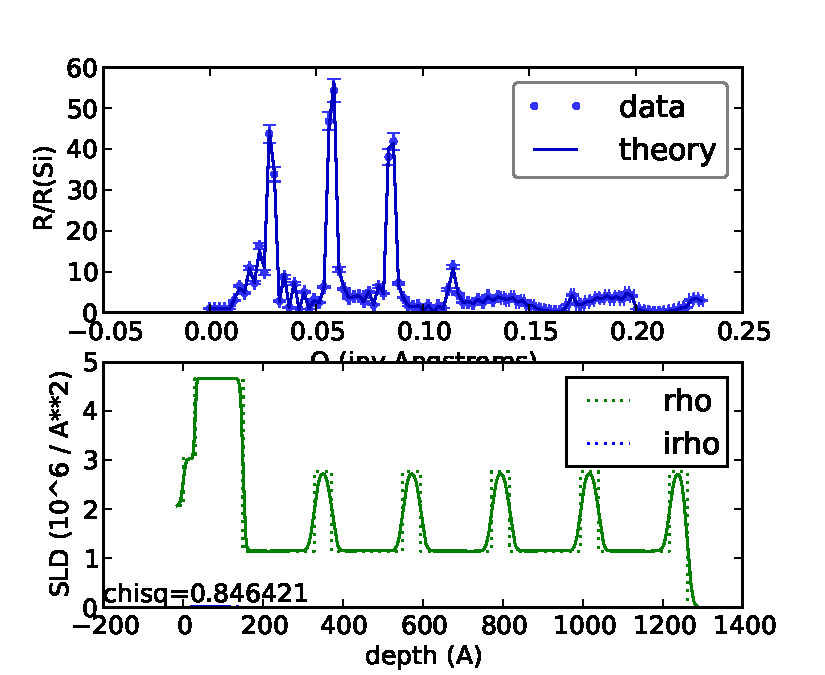
\includegraphics{a6b48bc7a5.pdf}

Bring in all of the functions from refl1d.names so that we can use them
in the remainder of the script.

\begin{Verbatim}[commandchars=@\[\]]
@PYGal[from] @PYGaW[refl1d.names] @PYGal[import] @PYGbe[*]
\end{Verbatim}

The polymer system is deposited on a gold film with chromium as an
adhesion layer. Because these are standard films which are very well-known
in this experiment we can use the built-in materials library to create
these layers.

\begin{Verbatim}[commandchars=@\[\]]
@PYGaE[@# == Sample definition ==]
chrome @PYGbe[=] Material(@PYGaB[']@PYGaB[Cr]@PYGaB['])
gold @PYGbe[=] Material(@PYGaB[']@PYGaB[Au]@PYGaB['])
\end{Verbatim}

The polymer system consists of two polymers, deuterated and non-deuterated
PDADMA/PSS.  Since the neutron scattering cross section for deuterium is
considerably different from that for hydrogen while having nearly identical
chemical properties, we can use the deuterium as a tag to see to what
extent the deuterated polymer layer interdiffuses with an underated polymer
layer.

We model the materials using scattering length density (SLD) rather than using
the chemical formula and mass density.  This allows us to fit the SLD directly
rather than making assumptions about the specific chemical composition of the
mixture.

\begin{Verbatim}[commandchars=@\[\]]
PDADMA@_dPSS @PYGbe[=] SLD(name @PYGbe[=]@PYGaB[']@PYGaB[PDADMA dPSS]@PYGaB['],rho @PYGbe[=] @PYGaw[2.77])
PDADMA@_PSS @PYGbe[=] SLD(name @PYGbe[=] @PYGaB[']@PYGaB[PDADMA PSS]@PYGaB['],rho @PYGbe[=] @PYGaw[1.15])
\end{Verbatim}

The polymer materials are stacked into a bilayer, with thickness
estimates based on ellipsometery measurements (as stated in the paper).

\begin{Verbatim}[commandchars=@\[\]]
bilayer @PYGbe[=] PDADMA@_PSS(@PYGaw[178],@PYGaw[10]) @PYGbe[@textbar[]] PDADMA@_dPSS(@PYGaw[44.3],@PYGaw[10])
\end{Verbatim}

The bilayer is repeated 5 times and stacked on the chromium/gold substrate
In this system we expect the kinetics of the surface diffusion to differ
from that of the bulk layer structure. Because we want the top bilayer to
optimise independently of the other bilayers, the fifth layer was not
included in the stack. If the diffusion properties of each layer were
expected to vary widely from one-another, the repeat notation could not
have been used at all.

\begin{Verbatim}[commandchars=@\[\]]
sample @PYGbe[=] (silicon(@PYGaw[0],@PYGaw[5]) @PYGbe[@textbar[]] chrome(@PYGaw[30],@PYGaw[3]) @PYGbe[@textbar[]] gold(@PYGaw[120],@PYGaw[5])
          @PYGbe[@textbar[]] (bilayer)@PYGbe[*]@PYGaw[4] @PYGbe[@textbar[]] PDADMA@_PSS(@PYGaw[178],@PYGaw[10]) @PYGbe[@textbar[]] PDADMA@_dPSS(@PYGaw[44.3],@PYGaw[10]) @PYGbe[@textbar[]] air)
\end{Verbatim}

Now that the model sample is built, we can start adding ranges to the fit
parameters. We assume that the chromium and gold layers are well known through
other methods and will not fit it; however, additional optimisation could
certainly be included here.

As stated earlier, we will be fitting the SLD of the polymers directly.
The range for each will vary from that for pure deuterated to the
pure undeuterated SLD.

\begin{Verbatim}[commandchars=@\[\]]
@PYGaE[@# == Fit parameters ==]
PDADMA@_dPSS@PYGbe[.]rho@PYGbe[.]range(@PYGaw[1.15],@PYGaw[2.77])
PDADMA@_PSS@PYGbe[.]rho@PYGbe[.]range(@PYGaw[1.15],@PYGaw[2.77])
\end{Verbatim}

We are primarily interested in the interfacial roughness so we will
fit those as well.  First we define the interfaces within the repeated
stack.  Note that the interface for bilayer{[}1{]} is the interface between
the current bilayer and the next bilayer.   Here we use sample{[}3{]} as
the repeated bilayer, which is the 0-origin index of the bilayer in the
stack.

\begin{Verbatim}[commandchars=@\[\]]
sample@PYGZlb[]@PYGaw[3]@PYGZrb[]@PYGZlb[]@PYGaw[0]@PYGZrb[]@PYGbe[.]interface@PYGbe[.]range(@PYGaw[5],@PYGaw[45])
sample@PYGZlb[]@PYGaw[3]@PYGZrb[]@PYGZlb[]@PYGaw[1]@PYGZrb[]@PYGbe[.]interface@PYGbe[.]range(@PYGaw[5],@PYGaw[45])
\end{Verbatim}

The interface between the stack and the next layer is controlled from
the repeated bilayer.

\begin{Verbatim}[commandchars=@\[\]]
sample@PYGZlb[]@PYGaw[3]@PYGZrb[]@PYGbe[.]interface@PYGbe[.]range(@PYGaw[5],@PYGaw[45])
\end{Verbatim}

Because the top bilayer has different dynamics, we optimize the interfaces
independenly. Although we want the optimiser to threat these parameters
independently because surface diffusion is expected to occur faster, the
overall nature of the diffusion is expected to be the same and so we use the
same limits.

\begin{Verbatim}[commandchars=@\[\]]
sample@PYGZlb[]@PYGaw[4]@PYGZrb[]@PYGbe[.]interface@PYGbe[.]range(@PYGaw[5],@PYGaw[45])
sample@PYGZlb[]@PYGaw[5]@PYGZrb[]@PYGbe[.]interface@PYGbe[.]range(@PYGaw[5],@PYGaw[45])
\end{Verbatim}

Finally we need to associate the sample with a measurement.  We do not
have the measurements from the paper available, so instead we will
simulate a measurement but setting up a neutron probe whose incident
angles range from 0 to 5 degrees in 100 steps.  The simulated measurement
is returned together with the model as a fit problem.

\begin{Verbatim}[commandchars=@\[\]]
@PYGaE[@# == Data ==]
T @PYGbe[=] numpy@PYGbe[.]linspace(@PYGaw[0], @PYGaw[5], @PYGaw[100])
probe @PYGbe[=] NeutronProbe(T@PYGbe[=]T, dT@PYGbe[=]@PYGaw[0.01], L@PYGbe[=]@PYGaw[4.75], dL@PYGbe[=]@PYGaw[0.0475])

M @PYGbe[=] Experiment(probe@PYGbe[=]probe, sample@PYGbe[=]sample)
M@PYGbe[.]simulate@_data(@PYGaw[5])

problem @PYGbe[=] FitProblem(M)
\end{Verbatim}


\subsection{Freeform structures}
\label{examples/superlattice/freeform:freeform-structures}\label{examples/superlattice/freeform::doc}
The following is a freeform superlattice floating in a solvent
and anchored with a tether molecule.  The tether is anchored via
a thiol group to a multilayer of Si/Cr/Au.  The sulphur in the
thiol attaches well to gold, but not silicon.  Gold will stick
to chrome which sticks to silicon.

Here is the plot using a random tether, membrane and tail group:

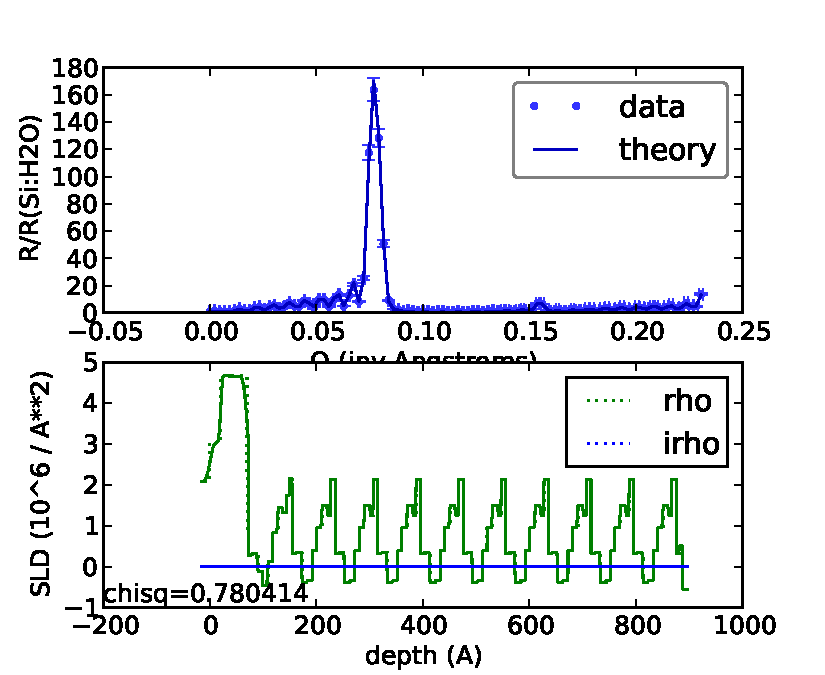
\includegraphics{1f37e03481.pdf}

The model is defined by \code{freeform.py}.

The materials are straight forward:

\begin{Verbatim}[commandchars=@\[\]]
@PYGal[from] @PYGaW[refl1d.names] @PYGal[import] @PYGbe[*]

chrome @PYGbe[=] Material(@PYGaB[']@PYGaB[Cr]@PYGaB['])
gold @PYGbe[=] Material(@PYGaB[']@PYGaB[Au]@PYGaB['])
solvent @PYGbe[=] Material(@PYGaB[']@PYGaB[H2O]@PYGaB['], density@PYGbe[=]@PYGaw[1])
\end{Verbatim}

The sample description is more complicated.  When we define a freeform
layer we need to anchor the ends of the freeform layer to a known
material.  Usually, this is just the material that makes up the preceding
and following layer.  In case we have freeform layers connected to each
other, though, we need an anchor material that controls the SLD at the
connection point.  For this purpose we introduce the dummy material
wrap

\begin{Verbatim}[commandchars=@\[\]]
wrap @PYGbe[=] SLD(name@PYGbe[=]@PYGaB["]@PYGaB[wrap]@PYGaB["], rho@PYGbe[=]@PYGaw[0])
\end{Verbatim}

Each section of the freeform layer has a different number of control
points.  The value should be large enough to give the profile enough
flexibility to match the data, but not so large that it over fits the
data.  Roughly the number of control points is the number of peaks and
valleys allowed.  We want a relatively smooth tether and tail, so we
keep \emph{n1} and \emph{n3} small, but make \emph{n2} large enough to define an
interesting repeat structure.

\begin{Verbatim}[commandchars=@\[\]]
n1, n2, n3 @PYGbe[=] @PYGaw[3],@PYGaw[9],@PYGaw[3]
\end{Verbatim}

Free layers have a thickness, horizontal control points \emph{z} varying
in $[0,1]$, real and complex SLD $\rho$ and $\rho_i$, and the material
above and below.

\begin{Verbatim}[commandchars=@\[\]]
tether @PYGbe[=] FreeLayer(below@PYGbe[=]gold, above@PYGbe[=]wrap, thickness@PYGbe[=]@PYGaw[10],
                   z@PYGbe[=]numpy@PYGbe[.]linspace(@PYGaw[0],@PYGaw[1],n1@PYGbe[+]@PYGaw[2])@PYGZlb[]@PYGaw[1]:@PYGbe[-]@PYGaw[1]@PYGZrb[],
                   rho@PYGbe[=]numpy@PYGbe[.]random@PYGbe[.]rand(n1),name@PYGbe[=]@PYGaB["]@PYGaB[tether]@PYGaB["])
bilayer @PYGbe[=] FreeLayer(below@PYGbe[=]wrap, above@PYGbe[=]wrap, thickness@PYGbe[=]@PYGaw[80],
                    z@PYGbe[=]numpy@PYGbe[.]linspace(@PYGaw[0],@PYGaw[1],n2@PYGbe[+]@PYGaw[2])@PYGZlb[]@PYGaw[1]:@PYGbe[-]@PYGaw[1]@PYGZrb[],
                    rho@PYGbe[=]@PYGaw[5]@PYGbe[*]numpy@PYGbe[.]random@PYGbe[.]rand(n2)@PYGbe[-]@PYGaw[1],name@PYGbe[=]@PYGaB["]@PYGaB[bilayer]@PYGaB["])
tail @PYGbe[=] FreeLayer(below@PYGbe[=]wrap, above@PYGbe[=]solvent, thickness@PYGbe[=]@PYGaw[10],
                   z@PYGbe[=]numpy@PYGbe[.]linspace(@PYGaw[0],@PYGaw[1],n3@PYGbe[+]@PYGaw[2])@PYGZlb[]@PYGaw[1]:@PYGbe[-]@PYGaw[1]@PYGZrb[],
                   rho@PYGbe[=]numpy@PYGbe[.]random@PYGbe[.]rand(n3),name@PYGbe[=]@PYGaB["]@PYGaB[tail]@PYGaB["])
\end{Verbatim}

With the predefined free layers, we can quickly define a stack, with
the bilayer repeat structure.  Note that we are setting the thickness
for the free layers when we define the layers, so there is no need to
set it when composing the layers into a sample.

\begin{Verbatim}[commandchars=@\[\]]
sample @PYGbe[=] (silicon(@PYGaw[0],@PYGaw[5]) @PYGbe[@textbar[]] chrome(@PYGaw[20],@PYGaw[2]) @PYGbe[@textbar[]] gold(@PYGaw[50],@PYGaw[5])
          @PYGbe[@textbar[]] tether @PYGbe[@textbar[]] bilayer@PYGbe[*]@PYGaw[10] @PYGbe[@textbar[]] tail @PYGbe[@textbar[]] solvent)
\end{Verbatim}

Finally, simulate the resulting model.

\begin{Verbatim}[commandchars=@\[\]]
T @PYGbe[=] numpy@PYGbe[.]linspace(@PYGaw[0], @PYGaw[5], @PYGaw[100])
probe @PYGbe[=] NeutronProbe(T@PYGbe[=]T, dT@PYGbe[=]@PYGaw[0.01], L@PYGbe[=]@PYGaw[4.75], dL@PYGbe[=]@PYGaw[0.0475],
                     back@_reflectivity@PYGbe[=]@PYGaA[True])
M @PYGbe[=] Experiment(probe@PYGbe[=]probe, sample@PYGbe[=]sample, dA@PYGbe[=]@PYGaw[5])
M@PYGbe[.]simulate@_data(@PYGaw[5])
problem @PYGbe[=] FitProblem(M)
\end{Verbatim}


\section{MLayer Models}
\label{examples/staj/readme:mlayer-models}\label{examples/staj/readme::doc}
This package can load models from other reflectometry fitting software.  In
this example we load an mlayer .staj file and fit the parameters within it.

The staj file can be used directly from the graphical interactor or it can
be previewed from the command line:

\begin{Verbatim}[commandchars=@\[\]]
@$ refl1d De2@_VATR.staj --preview
\end{Verbatim}

This shows the model plot:

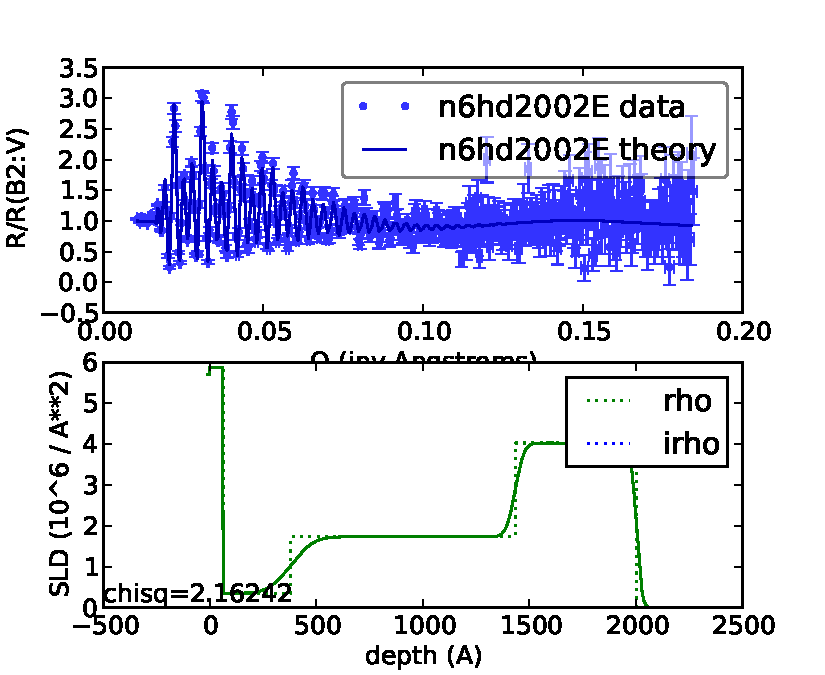
\includegraphics{aee62ada96.pdf}

and the available model parameters:

\begin{Verbatim}[commandchars=@\[\]]
.probe
  .back@_absorption = Parameter(1, name='back@_absorption')
  .background = Parameter(1e-10, name='background')
  .intensity = Parameter(1, name='intensity')
  .theta@_offset = Parameter(0, name='theta@_offset')
.sample
  .layers
    @PYGZlb[]0@PYGZrb[]
      .interface = Parameter(4.24661e-11, name='B3 interface')
      .material
        .irho = Parameter(3.00904e-05, name='B3 irho')
        .rho = Parameter(5.69228, name='B3 rho')
      .thickness = Parameter(90, name='B3 thickness')
    @PYGZlb[]1@PYGZrb[]
      .interface = Parameter(4.24661e-11, name='B2 interface')
      .material
        .irho = Parameter(1.39368e-05, name='B2 irho')
        .rho = Parameter(5.86948, name='B2 rho')
      .thickness = Parameter(64.0154, name='B2 thickness')
    @PYGZlb[]2@PYGZrb[]
      .interface = Parameter(83.7958, name='B1 interface')
      .material
        .irho = Parameter(6.93684e-05, name='B1 irho')
        .rho = Parameter(0.340309, name='B1 rho')
      .thickness = Parameter(316.991, name='B1 thickness')
    @PYGZlb[]3@PYGZrb[]
      .interface = Parameter(33.2095, name='M2 interface')
      .material
        .irho = Parameter(6.93684e-05, name='M2 irho')
        .rho = Parameter(1.73106, name='M2 rho')
      .thickness = Parameter(1052.77, name='M2 thickness')
    @PYGZlb[]4@PYGZrb[]
      .interface = Parameter(20.6753, name='M1 interface')
      .material
        .irho = Parameter(0.00137419, name='M1 irho')
        .rho = Parameter(4.02059, name='M1 rho')
      .thickness = Parameter(567.547, name='M1 thickness')
    @PYGZlb[]5@PYGZrb[]
      .interface = Parameter(4.24661e-11, name='V interface')
      .material
        .irho = Parameter(0, name='V irho')
        .rho = Parameter(0, name='V rho')
      .thickness = Parameter(0, name='V thickness')
  .thickness = stack thickness:2091.32

@PYGZlb[]chisq=2.16242, nllf=408.697@PYGZrb[]
\end{Verbatim}

Note that the parameters are reversed from the order in mlayer, so layer 0
is the substrate rather than the incident medium.  The graphical interactor,
refl1d\_gui, allows you to adjust parameters and fit ranges before starting
the fit, but you can also do so from a script, as shown in
\code{De2\_VATR.py}:

\begin{Verbatim}[commandchars=@\[\]]
@PYGal[from] @PYGaW[refl1d.names] @PYGal[import] @PYGbe[*]
@PYGal[from] @PYGaW[refl1d.stajconvert] @PYGal[import] load@_mlayer

@PYGaE[@# Load neutron model and data from staj file]
M @PYGbe[=] load@_mlayer(@PYGaB["]@PYGaB[De2@_VATR.staj]@PYGaB["])

@PYGaE[@# Set thickness/roughness fitting parameters to +/- 20 @%]
@PYGaE[@# Set SLD to +/- 5@% for all but the incident medium and the substrate.]
@PYGay[for] L @PYGav[in] M@PYGbe[.]sample@PYGZlb[]@PYGaw[1]:@PYGbe[-]@PYGaw[1]@PYGZrb[]:
    L@PYGbe[.]thickness@PYGbe[.]pmp(@PYGaw[20])
    L@PYGbe[.]interface@PYGbe[.]pmp(@PYGaw[20])
    L@PYGbe[.]material@PYGbe[.]rho@PYGbe[.]pmp(@PYGaw[5])

@PYGaE[@# Let the substrate SLD vary by 2@%]
M@PYGbe[.]sample@PYGZlb[]@PYGaw[0]@PYGZrb[]@PYGbe[.]material@PYGbe[.]rho@PYGbe[.]pmp(@PYGaw[2])
M@PYGbe[.]sample@PYGZlb[]@PYGaw[0]@PYGZrb[]@PYGbe[.]interface@PYGbe[.]range(@PYGaw[0],@PYGaw[20])
M@PYGbe[.]sample@PYGZlb[]@PYGaw[1]@PYGZrb[]@PYGbe[.]interface@PYGbe[.]range(@PYGaw[0],@PYGaw[20])

problem @PYGbe[=] FitProblem(M)
problem@PYGbe[.]name @PYGbe[=] @PYGaB["]@PYGaB[Desorption 2]@PYGaB["]
\end{Verbatim}

Staj file constraints are ignored, but you can get similar functionality by
setting parameters to equal expressions of other parameters.  You can even
constrain one staj file to share parameters with another by setting, for
example:

\begin{Verbatim}[commandchars=@\[\]]
M1 @PYGbe[=] load@_mlayer(@PYGaB["]@PYGaB[De1@_VATR.staj]@PYGaB["])
M2 @PYGbe[=] load@_mlayer(@PYGaB["]@PYGaB[De2@_VATR.staj]@PYGaB["])
M1@PYGbe[.]sample@PYGZlb[]@PYGaw[3]@PYGZrb[]@PYGbe[.]thickness @PYGbe[=] M2@PYGbe[.]sample@PYGZlb[]@PYGaw[3]@PYGZrb[]@PYGbe[.]thickness
problem @PYGbe[=] MultiFitProblem(@PYGZlb[]M1,M2@PYGZrb[])
\end{Verbatim}


\chapter{User's Guide}
\label{guide/index:user-s-guide}\label{guide/index::doc}\label{guide/index:users-guide-index}
Refl1D is a complex piece of software hiding some simple mathematics.
The reflectivity of a sample is a simple function of its optical
transform matrix $M$.  By slicing the sample in uniform layers, each
of which has a transfer matrix $M_i$, we can estimate the transfer
matrix for a depth-varying sample using $M=\prod M_i$.  We can
adjust the properties of the individual layers until the measured
reflectivity best matches the calculated reflectivty.

The complexity comes from multiple sources:
\begin{itemize}
\item {} 
Determining depth structure from reflectivity is an inverse problem
requiring a search through a landscape with multiple minima, whose
global minimum is small and often in an unpromising region.

\item {} 
The solution is not unique:  multiple minima may be equally valid
solutions to the inversion problem.

\item {} 
The measurement is sensitive to nuisance parameters such as sample
alignment.  That means the analysis program must include data
reduction steps, making data handling complicated.

\item {} 
The models are complex.  Since the ideal profile is not unique and
is difficult to locate, we often constrain our search to feasible
physical models to limit the search space, and to account for
information from other sources.

\item {} 
The reflectivity is dependent on the type of radiation used to probe
the sample and even its energy.

\end{itemize}

Introduction
\begin{quote}

Model scripts associate a sample description with data and fitting
options to define the system you wish to refine.
\end{quote}

Parameters
\begin{quote}

The adjustable values in each component of the system are defined
by {\hyperref[api/mystic.parameter:module-refl1d.mystic.parameter]{\code{Parameter}}} objects.  When you
set the range on a parameter, the system will be able to automatically
adjust the value in order to find the best match between theory
and data.
\end{quote}

Data
\begin{quote}

Data is loaded from instrument specific file
formats into a generic {\hyperref[api/probe:refl1d.probe.Probe]{\code{Probe}}}.  The
probe object manages the data view and by extension, the view of
the theory.  The probe object also knows the measurement resolution,
and controls the set of theory points that must be evaluated
in order to computed the expected value at each point.
\end{quote}

Materials
\begin{quote}

The strength of the interaction can be represented either in
terms of their scattering length density using
{\hyperref[api/material:refl1d.material.SLD]{\code{SLD}}}, or by their chemical
formula using {\hyperref[api/material:refl1d.material.Material]{\code{Material}}}, with
scattering length density computed from the information in the
probe.  {\hyperref[api/material:refl1d.material.Mixture]{\code{Mixture}}} can be used
to make a composite material whose parts vary be mass or by volume.
\end{quote}

Samples
\begin{quote}

Materials are composed into samples, usually as a
{\hyperref[api/model:refl1d.model.Stack]{\code{Stack}}} of
{\hyperref[api/model:refl1d.model.Slab]{\code{Slabs}}} layers, but more specific profiles
such as {\hyperref[api/polymer:refl1d.polymer.PolymerBrush]{\code{PolymerBrush}}}
are available.  Freeform sections of the profile can be described
using {\hyperref[api/mono:refl1d.mono.FreeLayer]{\code{FreeLayer}}}, allowing
arbitrary scattering length density profiles within the layer, or
{\hyperref[api/mono:refl1d.mono.FreeInterface]{\code{FreeInterface}}} allowing
arbitrary transitions from one SLD to another.  New layer types
can be defined by subclassing {\hyperref[api/model:refl1d.model.Layer]{\code{Layer}}}.
\end{quote}

Experiments
\begin{quote}

Sample descriptions and data sets are combined into an
{\hyperref[api/experiment:refl1d.experiment.Experiment]{\code{Experiment}}} object,
allowing the program to compute the expected reflectivity
from the sample and the probability that reflectivity measured
could have come from that sample.  For complex cases, where the
sample varies on a length scale larger than the coherence length
of the probe, you may need to model your measurement with a
\code{CompositeExperiment}.
\end{quote}

Fitting
\begin{quote}

One or more experiments can be combined into a
\code{FitProblem}.  This is then
given to one of the many fitters, such as
\code{PTFit}, which adjust the varying
parameters, trying to find the best fit.  PTFit can also
be used for Bayesian analysis in order to estimate the confidence
in which the parameter values are known.
\end{quote}


\section{Using Refl1D}
\label{guide/intro:intro-guide}\label{guide/intro:using-refl1d}\label{guide/intro::doc}
The Refl1D library is organized into modules.  Specific functions and
classes can be imported from a module, such as:

\begin{Verbatim}[commandchars=@\[\]]
@PYGaQ[@textgreater[]@textgreater[]@textgreater[] ]@PYGal[from] @PYGaW[refl1d.model] @PYGal[import] Slab
\end{Verbatim}

The most common imports have been gathered together in refl1d.names.  This
allows you to use names like {\hyperref[api/model:refl1d.model.Slab]{\code{Slab}}} directly:

\begin{Verbatim}[commandchars=@\[\]]
@PYGaQ[@textgreater[]@textgreater[]@textgreater[] ]@PYGal[from] @PYGaW[refl1d.names] @PYGal[import] @PYGbe[*]
@PYGaQ[@textgreater[]@textgreater[]@textgreater[] ]s @PYGbe[=] Slab(silicon, thickness@PYGbe[=]@PYGaw[100], interface)
\end{Verbatim}

This pattern of importing all names from a file,  while convenient for
simple scripts, makes the code more difficult to understand later, and
can lead to unexpected results when the same name is used in multiple
modules.  A safer, though more verbose pattern is to use:

\begin{Verbatim}[commandchars=@\[\]]
@PYGaQ[@textgreater[]@textgreater[]@textgreater[] ]@PYGal[import] @PYGaW[refl1d.names] @PYGal[as] @PYGaW[ref]
@PYGaQ[@textgreater[]@textgreater[]@textgreater[] ]s @PYGbe[=] ref@PYGbe[.]Slab(ref@PYGbe[.]silicon, thickness@PYGbe[=]@PYGaw[100], interface)
\end{Verbatim}

This documents to the reader unfamiliar with your code (such as you when
looking at your model files two years from now) exactly where the
name comes from.


\section{Parameters}
\label{guide/parameter::doc}\label{guide/parameter:parameter-guide}\label{guide/parameter:parameters}

\section{Data Representation}
\label{guide/data::doc}\label{guide/data:data-guide}\label{guide/data:data-representation}\setbox0\vbox{
\begin{minipage}{0.95\linewidth}
\begin{itemize}
\item {} 
{\hyperref[guide/data:simulated-probes]{Simulated probes}}

\item {} 
{\hyperref[guide/data:loading-data]{Loading data}}

\item {} 
{\hyperref[guide/data:viewing-data]{Viewing data}}

\item {} 
{\hyperref[guide/data:instrument-resolution]{Instrument Resolution}}

\item {} 
{\hyperref[guide/data:applying-resolution]{Applying Resolution}}

\item {} 
{\hyperref[guide/data:back-reflectivity]{Back reflectivity}}

\item {} 
{\hyperref[guide/data:alignment-offset]{Alignment offset}}

\item {} 
{\hyperref[guide/data:scattering-factors]{Scattering Factors}}

\end{itemize}
\end{minipage}}
\begin{center}\setlength{\fboxsep}{5pt}\shadowbox{\box0}\end{center}

Data is represented using {\hyperref[api/probe:refl1d.probe.Probe]{\code{Probe}}} objects.
The probe defines the Q values and the resolution of the individual
measurements, returning the scattering factors associated with the
different materials in the sample.  If the measurement has already
been performed, the probe stores the measured reflectivity and its
estimated uncertainty.

Probe objects are independent of the underlying instrument.  When
data is loaded, it is converted to angle $(\theta, \Delta \theta)$,
wavelength $(\lambda, \Delta \lambda)$ and reflectivity
$(R, \Delta R)$, with {\hyperref[api/probe:refl1d.probe.NeutronProbe]{\code{NeutronProbe}}}
used for neutron radiation and {\hyperref[api/probe:refl1d.probe.XrayProbe]{\code{XrayProbe}}}
used for X-ray radiation.  Additional properties,

Knowing the angle is necessary to correct for errors in sample alignment.


\subsection{Simulated probes}
\label{guide/data:simulated-probes}\label{guide/data:data-simulation}

\subsection{Loading data}
\label{guide/data:loading-data}\label{guide/data:data-loading}
For time-of-flight measurements, each angle should be represented as
a different probe.  This eliminates the `stitching' problem, where
$Q = 4 \pi \sin(\theta_1)/\lambda_1 = 4 \pi \sin(\theta_2)/\lambda_2$
for some $(\theta_1,\lambda_1)$ and $(\theta_2,\lambda_2)$.
With stitching, it is impossible to account for effects such as
alignment offset since two nominally identical Q values will in
fact be different.  No information is lost treating the two data sets
separately --- each points will contribute to the overall cost function
in accordance with its statistical weight.


\subsection{Viewing data}
\label{guide/data:data-views}\label{guide/data:viewing-data}
The probe object controls the plotting of theory and data curves.  This
is reasonable since it is only the probe which knows details such as
the original points and the points used in the calculation


\subsection{Instrument Resolution}
\label{guide/data:data-resolution}\label{guide/data:instrument-resolution}
With the instrument in a given configuration (\$theta\_i = theta\_f, lambda\$),
each neutron that is received is assigned to a particular $Q$ based on
the configuration.  However, these vaues are only nominal.  For example,
a monochromator lets in a range of wavelengths, and slits permit a range
of angles.  In effect, the reflectivity measured at the configuration
corresponds to a range of $Q$.

For monochromatic instruments, the wavelength resolution is fixed and
the angular resolution varies.  For polychromatic instruments, the
wavelength resolution varies and the angular resolution is fixed.
Resolution functions are defined in {\hyperref[api/resolution:module-refl1d.resolution]{\code{refl1d.resolution}}}.

The angular resolution is determined by the geometry (slit positions,
openings and sample profile) with perhaps an additional contribution
from sample warp.  For monochromatic instruments, measurements are taken
with fixed slits at low angles until the beam falls completely onto the
sample.  Then as the angle increases, slits are opened to preserve full
illumination.  At some point the slit openings exceed the beam width,
and thus they are left fixed for all angles above this threshold.

When the sample is tiny, stray neutrons miss the sample and are not
reflected onto the detector.  This results in a resolution that is
tighter than expected given the slit openings.  If the sample width
is available, we can use that to determine how much of the beam is
intercepted by the sample, which we then use as an alternative second
slit.  This simple calculation isn't quite correct for very low $Q$, but
data in this region will be contaminated by the direct beam, so we
won't be using those points.

When the sample is warped, it may act to either focus or spread the
incident beam.  Some samples are diffuse scatters, which also acts
to spread the beam.  The degree of spread can be estimated from the
full-width at half max (FWHM) of a rocking curve at known slit settings.
The expected FWHM will be $\frac{1}{2}(s_1+s_2)/(d_1-d_2)$.  The difference
between this and the measured FWHM is the sample\_broadening value.
A second order effect is that at low angles the warping will cast
shadows, changing the resolution and intensity in very complex ways.

For time of flight instruments, the wavelength dispersion
is determined by the reduction process which usually bins the time
channels in a way that sets a fixed relative resolution
$\Delta \lambda / \lambda$ for each bin.

Resolution in Q is computed from uncertainty in wavelength $\sigma_\lambda$
and angle $\sigma_\theta$ using propagation of errors:
\begin{gather}
\begin{split}\sigma^2_Q
    &= \left|\frac{\partial Q}{\partial \lambda}\right|^2 \sigma_\lambda^2
     + \left|\frac{\partial Q}{\partial \theta}\right|^2 \sigma_\theta^2
     + 2 \left|\frac{\partial Q}{\partial \lambda}
               \frac{\partial Q}{\partial \theta}\right|^2
               \sigma_{\lambda\theta}
     \\
Q &= 4 \pi \sin(\theta) / \lambda \\
\frac{\partial Q}{\partial \lambda} &= -4 \pi \sin(\theta)/\lambda^2
     = -Q/\lambda \\
\frac{\partial Q}{\partial \theta} &= 4 \pi \cos(\theta)/\lambda
     = \cos(\theta) \cdot Q/\sin(\theta) = Q/\tan(\theta)\end{split}\notag
\end{gather}
With no correlation between wavelength dispersion and angular divergence,
$\sigma_{\theta\lambda} = 0$, yielding the traditional form:
\begin{gather}
\begin{split}\left(\frac{\Delta Q}{Q}\right)^2
     = \left(\frac{\Delta \lambda}{\lambda}\right)^2
     + \left(\frac{\Delta \theta}{\tan(\theta)}\right)^2\end{split}\notag
\end{gather}
Computationally, $1/\tan(\theta) \rightarrow \infty$ at $\theta=0$, so
it is better to use the direct calculation:
\begin{gather}
\begin{split}\Delta Q = 4 \pi/\lambda \sqrt{\sin(\theta)^2 (\Delta\lambda/\lambda)^2
                               + \cos(\theta)^2 \Delta \theta^2}\end{split}\notag
\end{gather}
Wavelength dispersion $\Delta \lambda/\lambda$ is usually constant
(e.g., for AND/R it is 2\% FWHM), but it can vary on time-of-flight
instruments depending on how the data is binned.

Angular divergence $\delta \theta$ comes primarily from the slit geometry,
but can have broadening or focusing due to a warped sample.  The FWHM
divergence in radians due to slits is:
\begin{gather}
\begin{split}\Delta\theta_{\rm slits} = \frac{1}{2} \frac{s_1 + s_2}{d_1 - d_2}\end{split}\notag
\end{gather}
where $s_1,s_2$ are slit openings edge to edge and $d_1,d_2$ are the distances
between the sample and the slits.  For tiny samples of width $m$, the sample
itself can act as a slit.  If $s = m \sin(\theta)$ is smaller than $s_2$ for
some $\theta$, then use:
\begin{gather}
\begin{split}\Delta\theta_{\rm slits} = \frac{1}{2} \frac{s_1 + m \sin(\theta)}{d_1}\end{split}\notag
\end{gather}
The sample broadening can be read off a rocking curve using:
\begin{gather}
\begin{split}\Delta\theta_{\rm sample} = w - \Delta\theta_{\rm slits}\end{split}\notag
\end{gather}
where $w$ is the measured FWHM of the peak in degrees. Broadening can be
negative for concave samples which have a focusing effect on the beam.  This
constant should be added to the computed $\Delta \theta$ for all angles and
slit geometries.  You will not usually have this information on hand, but
you can leave space for users to enter it if it is available.

FWHM can be converted to 1-$\sigma$ resolution using the scale factor of
$1/\sqrt{8 \ln 2}$.

With opening slits we assume $\Delta \theta/\theta$ is held constant, so if
you know $s$ and $\theta_o$ at the start of the opening slits region you
can compute $\Delta \theta/\theta_o$, and later scale that to your
particular $\theta$:
\begin{gather}
\begin{split}\Delta\theta(Q) = \Delta\theta/\theta_o \cdot \theta(Q)\end{split}\notag
\end{gather}
Because $d$ is fixed, that means
$s_1(\theta) = s_1(\theta_o) \cdot \theta/\theta_o$ and
$s_2(\theta) = s_2(\theta_o) \cdot \theta/\theta_o$.


\subsection{Applying Resolution}
\label{guide/data:applying-resolution}\label{guide/data:data-resolution-calculator}
The instrument resolution is applied to the theory calculation on
a point by point basis using a value of $\Delta Q$ derived from
$\Delta\lambda$ and $\Delta\theta$.   Assuming the resolution is
well approximated by a Gaussian,
{\hyperref[api/reflectivity:refl1d.reflectivity.convolve]{\code{convolve}}} applies it to the
calculated theory function.

The convolution at each point $k$ is computed from the piece-wise linear
function $\bar R_i(q)$ defined by the refectivity $R(Q_i)$ computed
at points $Q_i \in Q_\text{calc}$
\begin{gather}
\begin{split}\bar R_i(q) &= m_i q + b_i \\
m_i &= (R_{i+1} - R_i)/(Q_{i+1} - Q_i) \\
b_i &= R_i - m_i Q_i\end{split}\notag
\end{gather}
and the Gaussian of width $\sigma_k = \Delta Q_k$
\begin{gather}
\begin{split}G_k(q) = \frac{1}{\sqrt{2 \pi}\sigma_k} e^{(q-Q_k)^2 / (2 \sigma_k^2)}\end{split}\notag
\end{gather}
using the piece-wise integral
\begin{gather}
\begin{split}\hat R_k = \sum_{i=i_\text{min}}^{i_\text{max}}
    \int_{Q_i}^{Q_{i+1}} \bar R_i(q) G_k(q) dq\end{split}\notag
\end{gather}
The range $i_\text{min}$ to $i_\text{max}$ for point $k$ is defined
to be the first $i$ such that $G_k(Q_i) < 0.001$, which is
about $3 \Delta Q_k$ away from $Q_k$.

By default the calculation points $Q_\text{calc}$ are the same
nominal $Q$ points at which the reflectivity was measured.   If the
data was measured densely enough, then the piece-wise linear function
$\bar R$ will be a good approximation to the underlying reflectivity.
There are two places in particular where this assumption breaks down.
One is near the critical edge for a sample that has sharp interfaces,
where the reflectivity drops precipitously. The other is in thick
samples, where the Kissig fringes are so close together that the
instrument cannot resolve them separately.

The method \code{Probe.critical\_edge()} fills in calculation points
near the critical edge.  Points are added linear around $Q_c$ for
a range of $\pm \delta Q_c$.  Thus, if the backing medium SLD or
the theta offset are allowed to vary a little during the fit, the
region after the critical edge may still be over-sampled.
The method \code{Probe.oversample()} fills in calculation points
around every point, giving each $\hat R$ a firm basis of support.

While the assumption of Gaussian resolution is reasonable on fixed
wavelength instruments, it is less  so on time of flight instruments,
which have asymmetric wavelength  distributions.  You can explore the
effects of different distributions by subclassing
{\hyperref[api/probe:refl1d.probe.Probe]{\code{Probe}}}  and overriding the
\code{\_apply\_resolution} method.  We will happily accept code for
improved resolution calculators and non-gaussian convolution.


\subsection{Back reflectivity}
\label{guide/data:back-reflectivity}\label{guide/data:data-backrefl}
While reflectivity is usually performed from the sample surface,
there are many instances where them comes instead through the
substrate.  For example, when the sample is soaked in water or
${\rm D}_2{\rm O}$, a neutron beam will not penetrate well and
it is better to measure the sample through the substrate.  Rather
than reversing the sample representation, these datasets can
be flagged with the attribute \emph{back\_reflectivity=True}, and the
sample constructed from substrate to surface as usual.

When the beam enters the side of the substrate, there is a
small refractive shift in $Q$ based on the angle of the beam relative
to the side of the substrate. The refracted beam reflects off the
the reversed film then exits the substrate on the other side, with an
opposite refractive shift.  Depending on the absorption coefficient
of the substrate, the beam will be attenuated in the process.

The refractive shift and the reversing of the film are automatically
handled by the underlying reflectivity calculation.  You can even
combine measurements through the sample surface and the substrate
into a single measurement, with negative $Q$ values representing
the transition from surface to substrate.  This is not uncommon with
magnetic thin film samples.

Usually the absorption effects of the substrate are accounted for
by measuring the incident beam through the same substrate before
normalizing the reflectivity.  There is a slight difference in path
length through the substrate depending on angle, but it is not
significant.  When this is not the case, particularly for measurements
which cross from the surface to substrate in the same scan, an
additional \emph{back\_absorption} parameter can be used to scale the
back reflectivity relative to the surface reflectivity.  There
is an overall \emph{intensity} parameter which scales both the surface
and the back reflectivity.

The interaction between \emph{back\_reflectivity}, \emph{back\_absorption},
sample representation and $Q$ value can be somewhat tricky.  It


\subsection{Alignment offset}
\label{guide/data:alignment-offset}\label{guide/data:data-alignment}
It can sometimes be difficult to align the sample, particularly on
X-ray instruments.  Unfortunately, a misaligned sample can lead to
a error in the measured position of the critical edge.  Since the
statistics for the measurement are very good in this region, the
effects on the fit can be large.  By representing the angle directly,
an alignment offset can be incorporated into the reflectivity calculation.
Furthermore, the uncertainty in the alignment can be estimated from
the alignment scans, and this information incorporated directly into
the fit.  Without the theta offset correction you would need to
compensate for the critical edge by allowing the scattering length
density of the substrate to vary during the fit, but this would lead to
incorrectly calculated reflectivity for the remaining points.  For
example, the simulation \code{toffset.py} shows more than 5\% error
in reflectivity for a silicon substrate with a 0.005° offset.

The method
{\hyperref[api/probe:refl1d.probe.Probe.alignment_uncertainty]{\code{Probe.alignment\_uncertainty}}}
computes the uncertainty in a alignment from the information in a
rocking curve.  The alignment itself comes from the peak position in
the rocking curve, with uncertainty determined from the uncertainty
in the peak position.  Note that this is not the same as the width
of the peak; the peak stays roughly the same width as statistics are
improved, but the uncertainty in position and width will
decrease.\footnote{
M.R. Daymond, P.J. Withers and M.W. Johnson;
The expected uncertainty of diffraction-peak location'',
Appl. Phys. A 74 {[}Suppl.{]}, S112 - S114 (2002).
\href{http://dx.doi.org/10.1007/s003390201392}{http://dx.doi.org/10.1007/s003390201392}
} There is an additional uncertainty in
alignment due to motor step size, easily computed from the
variance in a uniform distribution.  Combined, the uncertainty
in \emph{theta\_offset} is:
\begin{gather}
\begin{split}\Delta\theta \approx \sqrt{w^2/I + d^2/12}\end{split}\notag
\end{gather}
where $w$ is the full-width of the peak in radians at half maximum,
$I$ is the integrated intensity under the peak and $d$ is the motor
step size is radians.


\subsection{Scattering Factors}
\label{guide/data:scattering-factors}\label{guide/data:data-scattering-factors}
The effective scattering length density of the material is dependent
on the composition of the material and on the type and wavelength of
the probe object.  Using the chemical formula,
{\hyperref[api/probe:refl1d.probe.Probe.scattering_factors]{\code{scattering\_factors}}}
computes the scattering factors (\$rho\$, $\rho_i$, $\rho_{\rm inc}$)
associated with the material.  This means the same sample representation
can be used for X-ray and neutron experiments, with mass density as the
fittable parameter.  For energy dependent materials (e.g., Gd for neutrons),
then scattering factors will be returned for all of the energies in the
probe. (Note: energy dependent neutron scattering factors are not yet
implemented in periodic table.)

The returned scattering factors are normalized to density=1 g·cm$^{\text{-3}}$.
To use these values in the calculation of reflectivity, they need to
be scaled by density and volume fraction.  Using normalized density,
the value returned by scattering\_factors can be cached so only one
lookup is necessary during the fit even when density is a fitting
parameter.

The material itself can be flagged to use the incoherent scattering
factor $\rho_{\rm inc}$ which is by default ignored.

Magnetic scattering factors for the material are not presently
available in the periodic table.  Interested parties may consider
extending periodic table with magnetic scattering information and
adding support to
{\hyperref[api/probe:refl1d.probe.PolarizedNeutronProbe]{\code{PolarizedNeutronProbe}}}


\section{Materials}
\label{guide/materials:materials-guide}\label{guide/materials:materials}\label{guide/materials::doc}
Because this
is elemental nickel, we already know it's density.  For compounds
such as `SiO2' we would have to specify an additional
\code{density=2.634} parameter.

Common materials defined in {\hyperref[api/materialdb:module-refl1d.materialdb]{\code{materialdb}}}:
\begin{quote}

\emph{air}, \emph{water}, \emph{silicon}, \emph{sapphire}, ...
\end{quote}

Specific elements, molecules or mixtures can be added using the
classes in {\hyperref[api/material:module-refl1d.material]{\code{refl1d.material}}}:
\begin{quote}

\emph{SLD}       unknown material with fittable SLD
\emph{Material}  known chemical formula and fittable density
\emph{Mixture}   known alloy or mixture with fittable fractions
\end{quote}


\section{Sample Representation}
\label{guide/sample::doc}\label{guide/sample:sample-guide}\label{guide/sample:sample-representation}\setbox0\vbox{
\begin{minipage}{0.95\linewidth}
\begin{itemize}
\item {} 
{\hyperref[guide/sample:stacks]{Stacks}}

\item {} 
{\hyperref[guide/sample:multilayers]{Multilayers}}

\item {} 
{\hyperref[guide/sample:interfaces]{Interfaces}}

\item {} 
{\hyperref[guide/sample:slabs]{Slabs}}

\item {} 
{\hyperref[guide/sample:magnetic-layers]{Magnetic layers}}

\item {} 
{\hyperref[guide/sample:polymer-layers]{Polymer layers}}

\item {} 
{\hyperref[guide/sample:functional-layers]{Functional layers}}

\item {} 
{\hyperref[guide/sample:freeform-layers]{Freeform layers}}
\begin{itemize}
\item {} 
{\hyperref[guide/sample:comparison-of-models]{Comparison of models}}

\item {} 
{\hyperref[guide/sample:future-work]{Future work}}

\end{itemize}

\item {} 
{\hyperref[guide/sample:subclassing-layer]{Subclassing Layer}}

\end{itemize}
\end{minipage}}
\begin{center}\setlength{\fboxsep}{5pt}\shadowbox{\box0}\end{center}


\subsection{Stacks}
\label{guide/sample:stacks}
Reflectometry samples consist of 1-D stacks of layers joined by error
function interfaces. The layers themselves may be uniform slabs, or
the scattering density may vary with depth in the layer.  The first
layer in the stack is the substrate and the final layer is the surface.
Surface and substrate are assumed to be semi-infinite, with any thickness
ignored.


\subsection{Multilayers}
\label{guide/sample:multilayers}

\subsection{Interfaces}
\label{guide/sample:interfaces}
The interface between layers is assumed to smoothly follow and
error function profile to blend the layer above with the layer below.
The interface value is the 1-$\sigma$ gaussian roughness.
Adjacent flat layers with zero interface will act like a step function,
while positive values will introduce blending between the layers.

Blending is usually done with the Nevot-Croce formalism, which scales
the index of refraction between two layers by $\exp(-2 k_n k_{n+1} \sigma^2)$.
We show both a step function profile for the interface, as well as the
blended interface.

\begin{notice}{note}{Note:}
The blended interface representation is limited to the neighbouring
layers, and is not an accurate representation of the effective
reflectivity profile when the interface value is large relative to
the thickness of the layer.
\end{notice}

We will have a mechanism to force the use of the blended profile for
direct calculation of the interfaces rather than using the interface
scale factor.


\subsection{Slabs}
\label{guide/sample:slabs}
Materials can be stacked as slabs, with a thickness for each layer and
roughness at the top of each layer.  Because this is such a common
operation, there is special syntax to do it, using `\textbar{}' as the layer
separator and \emph{()} to specify thickness and interface.  For example,
the following is a 30 Å gold layer on top of silicon, with a
silicon:gold interface of 5 Å and a gold:air interface of 2 Å:

\begin{Verbatim}[commandchars=@\[\]]
@textgreater[]@textgreater[] from refl1d import *
@textgreater[]@textgreater[] sample = silicon(0,5) @textbar[] gold(30,2) @textbar[] air
@textgreater[]@textgreater[] print sample
Si @textbar[] Au(30) @textbar[] air
\end{Verbatim}

Individual layers and stacks can be used in multiple models, with all
parameters shared except those that are explicitly made separate.  The
syntax for doing so is similar to that for lists.  For example, the
following defines two samples, one with Si+Au/30+air and the other with
Si+Au/30+alkanethiol/10+air, with the silicon/gold layers shared:

\begin{Verbatim}[commandchars=@\[\]]
@textgreater[]@textgreater[] alkane@_thiol = Material('C2H4OHS',bulk@_density=0.8,name='thiol')
@textgreater[]@textgreater[] sample1 = silicon(0,5) @textbar[] gold(30,2) @textbar[] air
@textgreater[]@textgreater[] sample2 = sample1@PYGZlb[]:-1@PYGZrb[] @textbar[] alkane@_thiol(10,3) @textbar[] air
@textgreater[]@textgreater[] print sample2
Si @textbar[] Au(30) @textbar[] thiol(10) @textbar[] air
\end{Verbatim}

Stacks can be repeated using a simple multiply operation.  For example,
the following gives a cobalt/copper multilayer on silicon:

\begin{Verbatim}[commandchars=@\[\]]
@textgreater[]@textgreater[] Cu = Material('Cu')
@textgreater[]@textgreater[] Co = Material('Co')
@textgreater[]@textgreater[] sample = Si @textbar[] @PYGZlb[]Co(30) @textbar[] Cu(10)@PYGZrb[]*20 @textbar[] Co(30) @textbar[] air
@textgreater[]@textgreater[] print sample
Si @textbar[] @PYGZlb[]Co(30) @textbar[] Cu(10)@PYGZrb[]*20 @textbar[] Co(30) @textbar[] air
\end{Verbatim}

Multiple repeat sections can be included, and repeats can contain repeats.
Even freeform layers can be repeated.  By default the interface between
the repeats is the same as the interface between the repeats and the cap.
The cap interface can be set explicitly.  See \code{model.Repeat} for
details.


\subsection{Magnetic layers}
\label{guide/sample:magnetic-layers}

\subsection{Polymer layers}
\label{guide/sample:polymer-layers}

\subsection{Functional layers}
\label{guide/sample:functional-layers}

\subsection{Freeform layers}
\label{guide/sample:freeform-layers}
Freeform profiles allow us to adjust the shape of the depth profile using
control parameters.  The profile can directly represent the scattering
length density as a function of depth (a FreeLayer), or the relative
fraction of one material and another (a FreeInterface).  With a freeform
interface you can simultaneously fit two systems which should share the
same volume profile but whose materials have different scattering length
densities.  For example, a polymer in deuterated and undeuterated solvents
can be simultaneously fit with freeform profiles.

We have multiple representations for freeform profiles, each with its
own strengths and weaknesses:
\begin{itemize}
\item {} 
\href{http://en.wikipedia.org/wiki/Monotone\_cubic\_interpolation}{monotone cubic interpolation}
({\hyperref[api/mono:module-refl1d.mono]{\code{refl1d.mono}}})

\item {} 
\href{http://en.wikipedia.org/wiki/B-spline}{parameteric B-splines}
({\hyperref[api/freeform:module-refl1d.freeform]{\code{refl1d.freeform}}})

\item {} \begin{description}
\item[{{\color{red}\bfseries{}{}`}Chebyshev interpolating polynomials}] \leavevmode
\textless{}\href{http://en.wikipedia.org/wiki/Chebyshev\_polynomials}{http://en.wikipedia.org/wiki/Chebyshev\_polynomials}\textgreater{}{}`\_
({\hyperref[api/cheby:module-refl1d.cheby]{\code{refl1d.cheby}}})

\end{description}

\end{itemize}

At present, monotone cubic interpolation is the most developed, but work
on all representations is in flux.  In particular not every representation
supports all features, and the programming interface may vary. See the
documentation for the individual models for details.


\subsubsection{Comparison of models}
\label{guide/sample:comparison-of-models}
There are a number of issues surrounding the choice of model.
\begin{itemize}
\item {} 
How easy is it to bound the profile values

If the you can put reasonable bounds on the control points, then the
user can bring to bear prior information to limit the search space.
For example, it is common to add an unknown silicon-oxide profile
to the surface of silicon, with SLD varying between the values for
Si and SiO$_{\text{2}}$

\item {} 
How easy is it to edit the profile interactively

Given a representation of the freeform layer, we want to be able to
plot control points that you can drag in order to change the shape
of the profile.

\item {} 
Is the profile stable or does it oscillate wildly

Many systems are best described by smoothly varying density profiles.
If the profile oscillates wildly it makes the search for optimal
parameters more difficult.

\item {} 
Can you change the order of interpolation and preserve the profile

While the current code does not support it, we would like to be
able to select the freeform profile order automatically, using the
minimum order we can to achieve $\chi^2 = 1$, and rejecting profiles
which overfit the data.  For now this is done by hand, performing
fits with different orders independently, but there are likely to
be speed gains by first fitting coarse models with low Q then adding
detail to the profile while adding additional Q values.

\item {} 
Is the representation unique?  Are the control parameters strongly
correlated?

Fitting and uncertainty analysis benefit from unique solutions.  If
the model representation is matched by a family of parameters it is
more difficult to interpret the results of the uncertainty analysis
or to get convergence from the parameter refinement engine.

\end{itemize}

Monotone cubic interpolation is the easiest to control.  The value of the
interpolating polynomial lies mostly within the range of the control
points, and the profile goes through the control points.  This means
you can set up bounds on the control parameters that limit the profile
to a certain range of scattering length densities in a region of the
profile.  It also leads to a very intuitive interactive profile editor
since the control points can be moved directly on profile view.  However,
although the profile is $C^1$ smooth everywhere, the $C^2$ transitions
can be abrupt at the control points.  Better algorithms for selecting the
gradient exist but have not been implemented, so this may improve in
the future.

Parametric B-splines are commonly used in computer graphics because they
create pleasing curves.  The interpolating polynomial lies within the
convex hull of the control points.  Unfortunately the distance between the
curve and the control point can be large, and this makes it difficult
to set reasonable bounds on the values of the control points.  One can
reformulate the interpolation so that control points lie on the curve
and still preserve the property of pleasing curves, but this can lead
to wild oscillations in the profile when the control points become too
close together.  While the natural representation can be used in an
interactive profile editor, the fact that the control points are sometimes
far away from the profile makes this inconvenient.  The complementary
representation is used in programs such as Microsoft Excel, with the
control point directly on the curve and a secondary control point to
adjust the slope at that control point.

Chebyshev interpolating polynomials are a near optimal representation
for an function over an interval with respect to the maximum norm.  The
interpolating polynomial is a weighted sum $\sigma_{i=0}^n c_i T_i(z)$
of the Chebyshev basis polynomials $T_i$ with Chebyshev coefficients $c_i$.
One very interesting property is that the lower order coefficients remain
the same has higher order interpolation polynomials are constructed.
This makes the Chebyshev polynomials very interesting candidates for
a freeform profile fitter which selects the order of the profile as
part of the fit.  Chebyshev interpolating polynomials can exhibit
wild oscillations if the coefficients become large, so the smoothness
can be somewhat controlled by limiting these higher values, but we have
not explored this in depth. The Chebyshev coefficient values are not
directly tied to the profile, so there is no intuitive way to directly
control the coefficients in an interactive editor. The complementary
representation uses the profile value at the chebyshev nodes for
specific positions $z_i$ on the profile.  This representation is much
more natural for an interactive editor, but some choices of control
values will lead to wild oscillations between the nodes.  Similarly
the complementary representation is unsuitable as a representation
for the fittable parameters since the bounds on the parameters do
not directly limit the range of possible values of the profile.


\subsubsection{Future work}
\label{guide/sample:future-work}
We only have polynomial spline representations for our profiles.  Similar
profiles could be constructed from different basis functions such as
wavelets, the idea being to find a multiscale representation of your
profile and use model selection techniques to determine the most coarse
grained representation that matches your data.

Totally freeform representations as separately controlled microslab
heights would also be interesting in the context of a maximum entropy
fitting engine: find the smoothest profile which matches the data, for
some definition of `smooth'.  Some possible smoothness measures are the
mean squared distance from zero, the number of sign changes in the second
derivative, the sum of the absolute value of the first derivative, the
maximum flat region, the minimum number of flat slabs, etc.  Given that
reflectometry inversion is not unique, the smoothness measure must
correspond to the likelihood of finding the system in that particularly
state:  that is, don't expect your sample to show zebra stripes unless
you are on an African safari or visiting a zoo.


\subsection{Subclassing Layer}
\label{guide/sample:new-layers}\label{guide/sample:subclassing-layer}

\section{Experiment}
\label{guide/experiment:experiment}\label{guide/experiment::doc}\label{guide/experiment:experiment-guide}\setbox0\vbox{
\begin{minipage}{0.95\linewidth}
\begin{itemize}
\item {} 
{\hyperref[guide/experiment:direct-calculation]{Direct Calculation}}

\end{itemize}
\end{minipage}}
\begin{center}\setlength{\fboxsep}{5pt}\shadowbox{\box0}\end{center}

The {\hyperref[api/experiment:refl1d.experiment.Experiment]{\code{Experiment}}} object links a
sample with an experimental probe.
The probe defines the Q values and the resolution of the individual
measurements, and returns the scattering factors associated with the
different materials in the sample.

For the simple case of exploring the reflectivity of new samples,
this means that you must define

the
purposes:
\begin{itemize}
\item {} 
defining the instrument resolution

\item {} 
providing the scattering factors for materials

\end{itemize}

Because our models allow representation based on composition, it is no
longer trivial to compute the reflectivity from the model.  We now have
to look up the effective scattering density based on the probe type and
probe energy.  You've already seen this in the {\color{red}\bfseries{}{}`new\_layers{}`\_} section:
the render method for the layer requires the probe to look up the material
scattering factors.


\subsection{Direct Calculation}
\label{guide/experiment:direct-calculation}
Rather than using \code{Stack \textless{}refl1d.model.Stack},
{\hyperref[api/probe:refl1d.probe.Probe]{\code{Probe}}} and
class:\emph{Experiment \textless{}refl1d.experiment.Experiment},
we  can compute reflectivities directly with the functions in
{\hyperref[api/reflectivity:module-refl1d.reflectivity]{\code{refl1d.reflectivity}}}.  These routines provide the raw
calculation engines for the optical matrix formalism, converting
microslab models of the sample into complex reflectivity amplitudes,
and convolving the resulting reflectivity with the instrument resolution.

The following performs a complete calculation for a silicon
substrate with 5 Å roughness using neutrons.  The theory is sampled
at intervals of 0.001, which is convolved with a 1\% $\Delta Q/Q$ resolution
function to yield reflectivities at intervals of 0.01.

\begin{Verbatim}[commandchars=@\[\]]
@PYGaQ[@textgreater[]@textgreater[]@textgreater[] ]@PYGal[from] @PYGaW[numpy] @PYGal[import] arange
@PYGaQ[@textgreater[]@textgreater[]@textgreater[] ]@PYGal[from] @PYGaW[refl1d.reflectivity] @PYGal[import] reflectivity@_amplitude @PYGay[as] reflamp
@PYGaQ[@textgreater[]@textgreater[]@textgreater[] ]@PYGal[from] @PYGaW[refl1d.reflectivity] @PYGal[import] convolve
@PYGaQ[@textgreater[]@textgreater[]@textgreater[] ]Qin @PYGbe[=] arange(@PYGaw[0],@PYGaw[0.21],@PYGaw[0.001])
@PYGaQ[@textgreater[]@textgreater[]@textgreater[] ]w,rho,irho,sigma @PYGbe[=] @PYGaY[zip]((@PYGaw[0],@PYGaw[2.07],@PYGaw[0],@PYGaw[5]),(@PYGaw[0],@PYGaw[0],@PYGaw[0],@PYGaw[0]))
@PYGaQ[@textgreater[]@textgreater[]@textgreater[] ]r @PYGbe[=] reflamp(kz@PYGbe[=]Qin@PYGbe[/]@PYGaw[2], depth@PYGbe[=]w, rho@PYGbe[=]rho, irho@PYGbe[=]irho, sigma@PYGbe[=]sigma)
@PYGaQ[@textgreater[]@textgreater[]@textgreater[] ]Rin @PYGbe[=] (r@PYGbe[*]r@PYGbe[.]conj())@PYGbe[.]real
@PYGaQ[@textgreater[]@textgreater[]@textgreater[] ]Q @PYGbe[=] arange(@PYGaw[0],@PYGaw[0.2],@PYGaw[0.01])
@PYGaQ[@textgreater[]@textgreater[]@textgreater[] ]dQ @PYGbe[=] Q@PYGbe[*]@PYGaw[0.01] @PYGaE[@# resolution dQ/Q = 0.01]
@PYGaQ[@textgreater[]@textgreater[]@textgreater[] ]R @PYGbe[=] convolve(Qin, Rin, Q, dQ)
@PYGaQ[@textgreater[]@textgreater[]@textgreater[] ]@PYGay[print] @PYGaB["]@PYGao[\n]@PYGaB["]@PYGbe[.]join(@PYGaB["]@PYGaB[Q: ]@PYGbg[@%.2g]@PYGaB[  R: ]@PYGbg[@%.5g]@PYGaB["]@PYGbe[@%](Qi,Ri) @PYGay[for] Qi,Ri @PYGav[in] @PYGaY[zip](Q,R))
\end{Verbatim}


\section{Fitting}
\label{guide/fitting:fitting}\label{guide/fitting::doc}\label{guide/fitting:fitting-guide}\setbox0\vbox{
\begin{minipage}{0.95\linewidth}
\begin{itemize}
\item {} 
{\hyperref[guide/fitting:quick-fit]{Quick Fit}}

\item {} 
{\hyperref[guide/fitting:uncertainty-analysis]{Uncertainty Analysis}}

\item {} 
{\hyperref[guide/fitting:using-the-posterior-distribution]{Using the posterior distribution}}

\item {} 
{\hyperref[guide/fitting:tough-problems]{Tough Problems}}

\item {} 
{\hyperref[guide/fitting:command-line]{Command Line}}

\item {} 
{\hyperref[guide/fitting:other-optimizers]{Other optimizers}}

\item {} 
{\hyperref[guide/fitting:references]{References}}

\end{itemize}
\end{minipage}}
\begin{center}\setlength{\fboxsep}{5pt}\shadowbox{\box0}\end{center}

Obtaining a good fit depends foremost on having the correct model to fit.

Too many layers, too few layers, too limited fit ranges, too open fit
ranges, all of these can make fitting difficult.  For example, forgetting
the SiOx layer on the silicon substrate will distort the model of a
polymer film.

Even with the correct model, there are systematic errors to address
(see \emph{\_data\_guide}). A warped sample can lead to broader resolution than
expected near the critical edge, and \emph{sample\_broadening=value} must be
specified when loading the data.  Small errors in alignment of the sample or
the slits will move the measured critical edge, and so \emph{probe.theta\_offset}
may need to be fitted.  Points near the critical edge are difficult to
compute correctly with resolution because the reflectivity varies so quickly.
Using {\hyperref[api/probe:refl1d.probe.Probe.critical_edge]{\code{refl1d.probe.Probe.critical\_edge()}}}, the density of the
points used to compute the resolution near the critical edge can be
increased.  For thick samples  the resolution will integrate over
multiple Kissig fringes, and \code{refl1d.probe.Probe.over\_sample()}
will be needed to average across them and avoid aliasing effects.


\subsection{Quick Fit}
\label{guide/fitting:quick-fit}
While generating an appropriate model, you will want to perform a number
of quick fits.  The Nelder-Mead simplex algorithm (fit=amoeba) works well
for this.  You will want to run it with steps between 1000 and 3000 so
the algorithm has a chance to converge.  Restarting a number of times
(somewhere between 3 and 100) gives a reasonably thorough search of the
fit space.  From the graphical user interface (refl\_gui), using starts=1
and clicking the fit button to improve the fit as needed works pretty well.
From the command line interface (refl\_cli), the command line will be
something like:

\begin{Verbatim}[commandchars=@\[\]]
refl1d --fit=amoeba --steps=1000 --starts=20 --parallel model.py --store=T1
\end{Verbatim}

The command line result can be improved by using the previous fit value as
the starting point for the next fit:

\begin{Verbatim}[commandchars=@\[\]]
refl1d --fit=amoeba --steps=1000 --starts=20 --parallel model.py --store=T1 --pars=T1/model.par
\end{Verbatim}

Differential evolution (fit=de) and random lines (fit=rl) are alternatives
to amoeba, perhaps a little more likely to find the global minimum but
somewhat slower. These are population based algorithms in which several
points from the current population are selected, and based on their
position and value, a new point is generated.  The population is specified
as a multiplier on the number of parameters in the model, so for example
an 8 parameter model with DE's default population (pop=10) would create 80
points each generation.  Random lines with a large population is fast but
is not good at finding isolated minima away from the general trend, so its
population defaults to pop=0.5.  These algorithms can be called from the
command line as follows:

\begin{Verbatim}[commandchars=@\[\]]
refl1d --fit=de --steps=3000 --parallel model.py --store=T1
refl1d --fit=rl --steps=3000 --starts=200 --reset --parellel model.py --store=T1
\end{Verbatim}

Of course, --pars can be used to start from a previously completed fit.


\subsection{Uncertainty Analysis}
\label{guide/fitting:uncertainty-analysis}
More important than the optimal value of the parameters is an estimate
of the uncertainty in those values.  By casting our problem as the
likelihood of seeing the data given the model, we not only give
ourselves the ability to incorporate prior information into the fit
systematically, but we also give ourselves a strong foundation for
assessing the uncertainty of the parameters.

Uncertainty analysis is performed using DREAM (fit=dream).  This is a
Markov chain Monte Carlo (MCMC) method with a differential evolution
step generator.  Like simulated annealing, the MCMC explores the space
using a random walk, always accepting a better point, but sometimes
accepting a worse point depending on how much worse it is.

DREAM can be started with a variety of initial populations.  The
random population (init=random) distributes the initial points using
a uniform distribution across the space of the parameters.  Latin
hypersquares (init=lhs) improves on random by making sure that
there is on value for each subrange of every variable. The covariance
population (init=cov) selects points from the uncertainty ellipse
computed from the derivative at the initial point.  This method
will fail if the fitting parameters are highly correlated and the
covariance matrix is singular.  The epsilon ball population (init=eps)
starts DREAM from a tiny region near the initial point and lets it
expand from there.  It can be useful to start with an epsilon ball
from the previous best point when DREAM fails to converge using
a more diverse initial population.

The Markov chain will take time to converge on a stable population.
This burn in time needs to be specified at the start of the analysis.
After burn, DREAM will collect all points visited for N iterations
of the algorithm.  If the burn time was long enough, the resulting
points can be used to estimate uncertainty on parameters.

A common command line for running DREAM is:

\begin{Verbatim}[commandchars=@\[\]]
refl1d --fit=dream --burn=1000 --steps=1000 --init=cov --parallel --pars=T1/model.par model.py --store=T2
\end{Verbatim}

Bayesian uncertainty analysis us described in the GUM Supplement 1,{[}8{]}
and is a valid technique for reporting parameter uncertainties in NIST
publications.   Given sufficient burn time, points in the search space
will be visited with probability proportional to the goodness of fit.
The file T1/model.err contains a table showing for each
parameter the mean(std), median and best values, and the 68\% and 95\%
credible intervals.  The mean and standard deviation are computed from
all the samples in the returned distribution.  These statistics are not
robust: if the Markov process has not yet converged, then outliers will
significantly distort the reported values.  Standard deviation is
reported in compact notation, with the two digits in parentheses
representing uncertainty in the last two digits of the mean.  Thus, for
example, $24.9(28)$ is $24.9 \pm 2.8$.  Median is the best value in the
distribution.  Best is the best value ever seen.  The 68\% and 95\%
intervals are the shortest intervals that contain 68\% and 95\% of
the points respectively.  In order to report 2 digits of precision on
the 95\% interval, approximately 1000000 draws from the distribution
are required, or steps = 1000000/(\#parameters  \#pop).  The 68\% interval
will require fewer draws, though how many has not yet been determined.

\scalebox{0.500000}{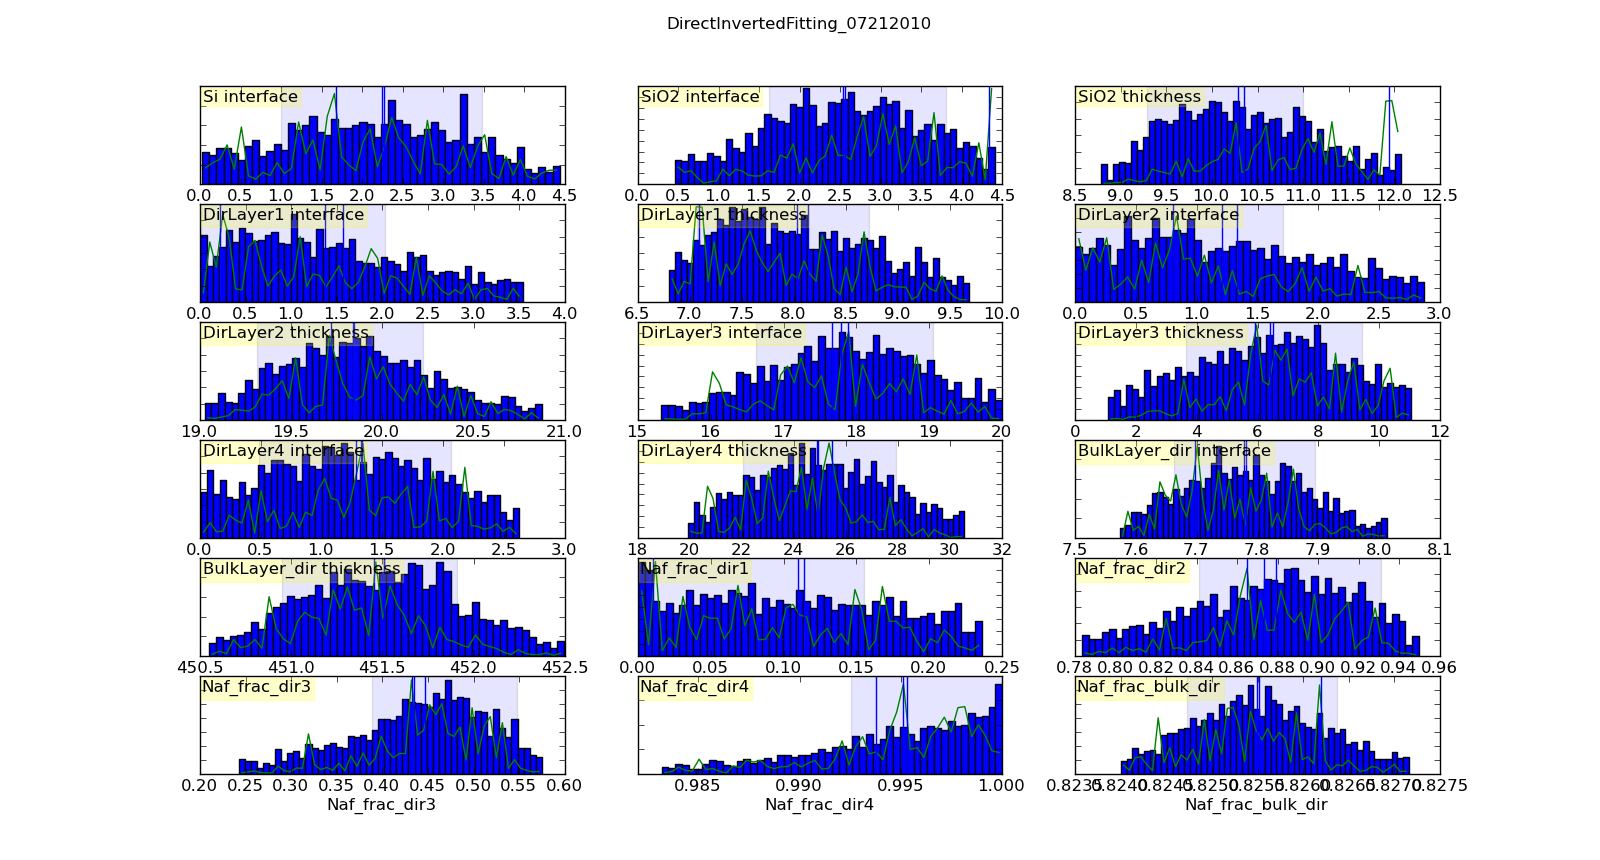
\includegraphics{var.png}}

Histogramming the set of points visited will gives a picture of the
probability density function for each parameter.  This histogram is
generated automatically and saved in T1/model-var.png.  The histogram
range represents the 95\% credible interval, and the shaded region
represents the 68\% credible interval.  The green line shows the highest
probability observed given that the parameter value is restricted to
that bin of the histogram.  With enough samples, this will correspond
to the maximum likelihood value of the function given that one parameter
is restricted to that bin.  In practice, the analysis has converged
when the green line follows the general shape of the histogram.

\scalebox{0.500000}{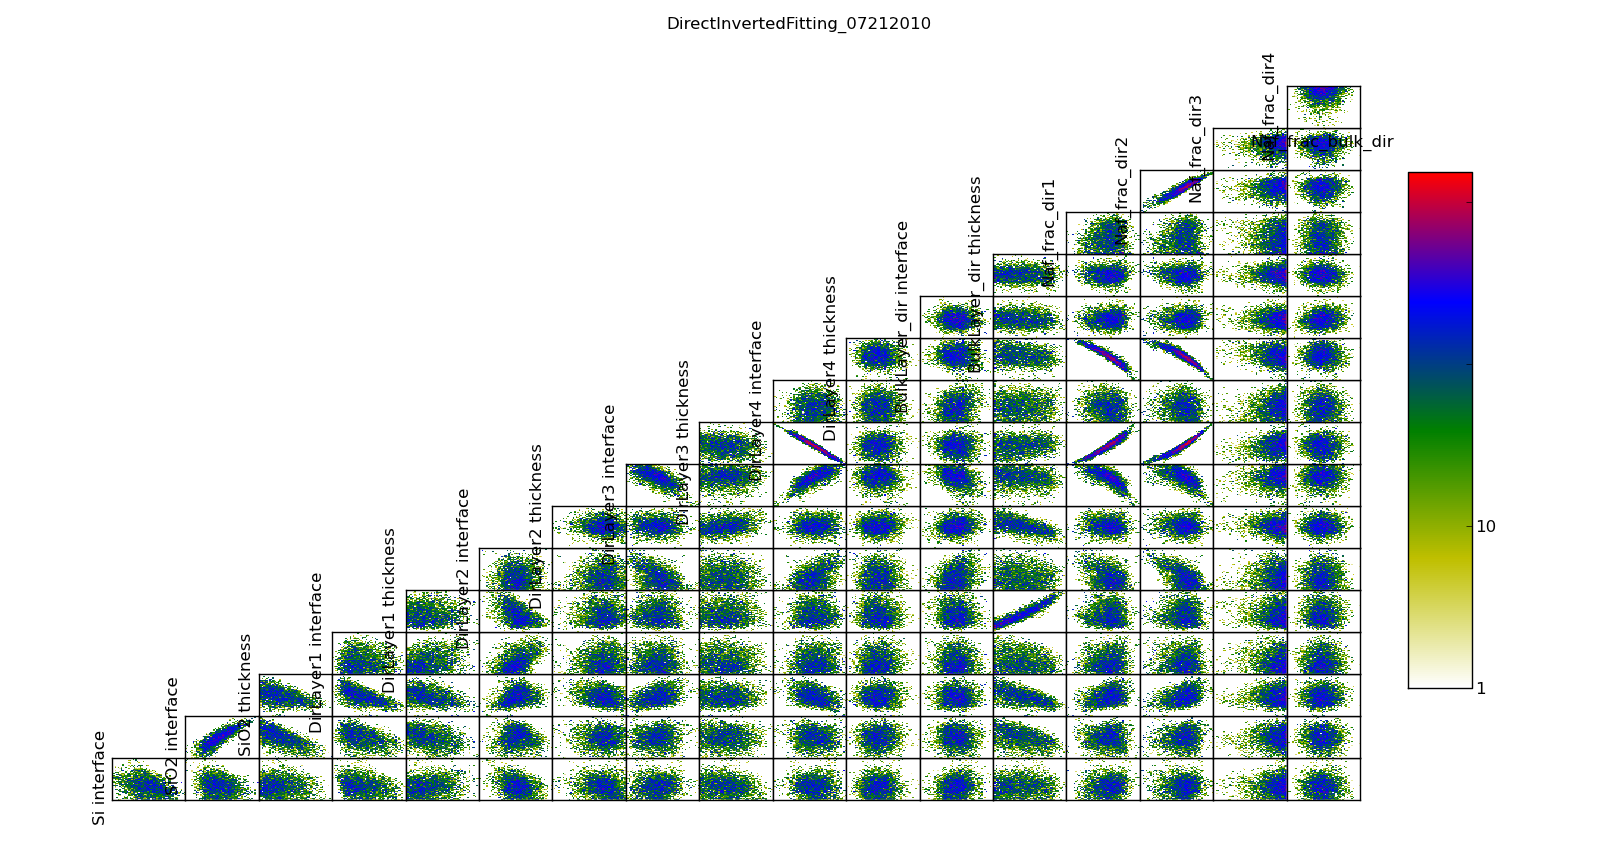
\includegraphics{corr.png}}

The correlation plots show that the parameters are not uniquely
determined from the data.  For example, the thickness of
lamellae 3 and 4 are strongly anti-correlated, yielding a 95\% CI of
about 1 nm for each compared to the bulk nafion thickness CI of 0.2 nm.
Summing lamellae thickness in the sampled points, we see the overall
lamellae thickness has a CI of about 0.3 nm.  The correlation
plot is saved in T1/model-corr.png.

\scalebox{0.500000}{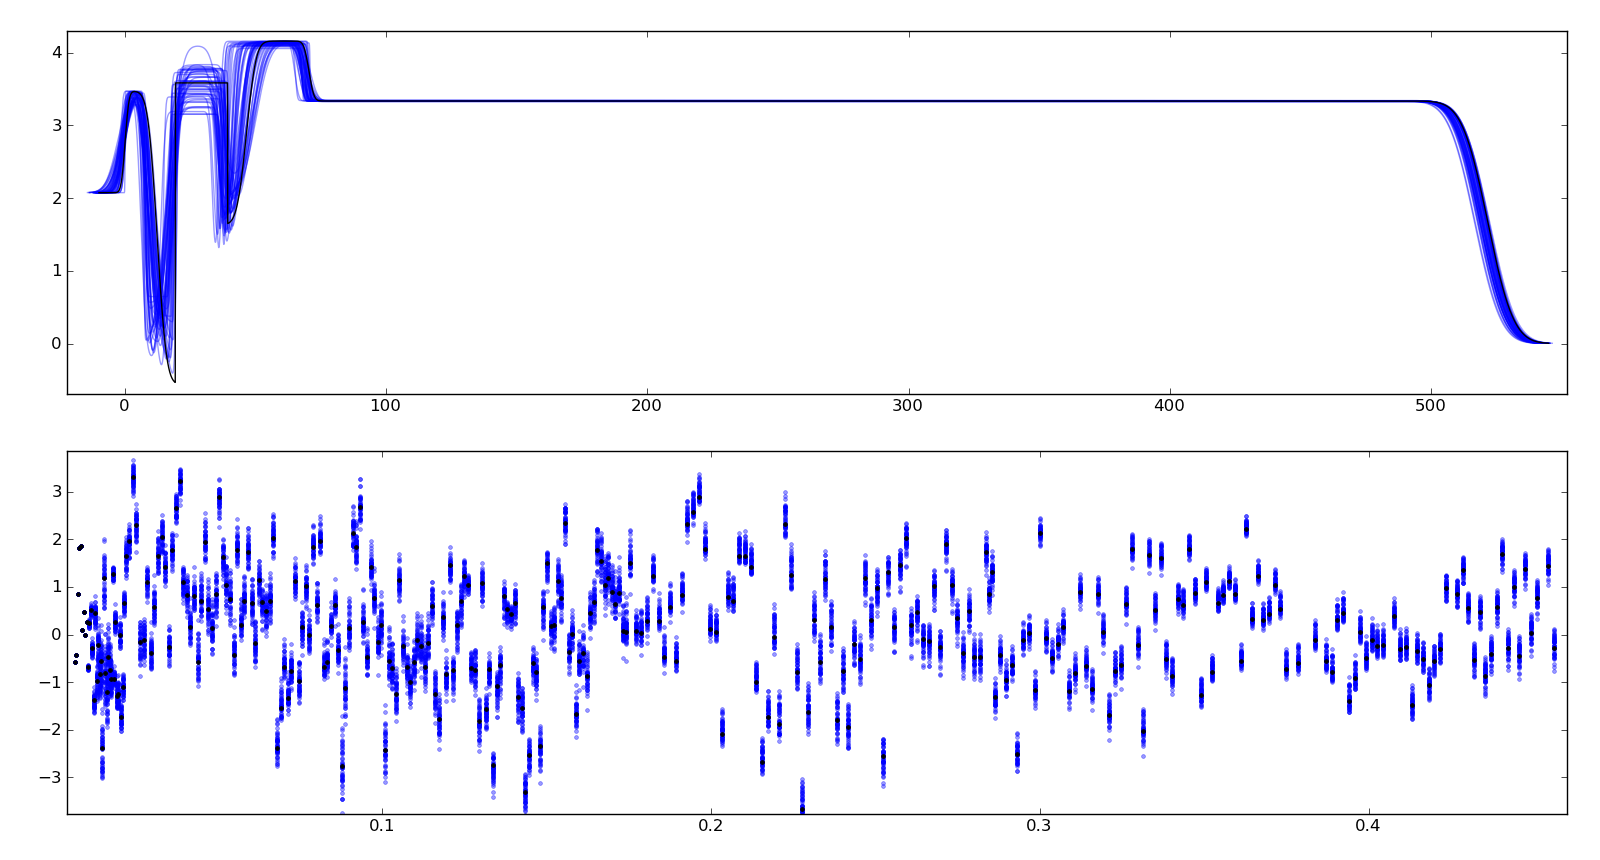
\includegraphics{error.png}}

To assure ourselves that the uncertainties produced by DREAM do
indeed correspond to the underlying uncertainty in the model, we perform
a Monte Carlo forward uncertainty analysis by selecting 50 samples from
the computed posterior distribution, computing the corresponding
reflectivity and calculating the normalized residuals.  Assuming that
our measurement uncertainties are approximately normally distributed,
approximately 68\% of the normalized residuals should be within +/- 1 of
the residual for the best model, and 98\% should be within +/- 2. Note
that our best fit does not capture all the details of the data, and the
underlying systematic bias is not included in the uncertainty estimates.

Plotting the profiles generated from the above sampling method, aligning
them such that the cross correlation with the best profile is maximized,
we see that the precise details of the lamellae are uncertain but the
total thickness of the lamellae structure is well determined.  Bayesian
analysis can also be used to determine relative likelihood of different
number of layers, but we have not yet performed this analysis.  This plot
is stored in T1/model-errors.png.

The trace plot, T1/model-trace.png, shows the mixing properties of the
first fitting parameter.  If the Markov process is well behaved, the
trace plot will show a lot of mixing.  If it is ill behaved, and each
chain is stuck in its own separate local minimum, then distinct lines
will be visible in this plot.

The convergence plot, T1/model-logp.png, shows the log likelihood
values for each member of the population.  When the Markov process
has converged, this plot will be flat with no distinct lines visible.
If it shows a general upward sweep, then the burn time was not
sufficient, and the analysis should be restarted.  The ability to
continue to burn from the current population is not yet implemented.

Just because all the plots are well behaved does not mean that the
Markov process has converged on the best result.  It is practically
impossible to rule out a deep minimum with a narrow acceptance
region in an otherwise unpromising part of the search space.

In order to assess the DREAM algorithm for suitability for reflectometry
fitting we did a number of tests.  Given that the fit surface is
multimodal, we need to know that the uncertainty analysis can return
multiple modes.  Because the fit problems may also be ill-conditioned,
with strong correlations or anti-correlations between some parameters,
the uncertainty analysis  needs to be able to correctly indicate that
the correlations exist. Simple Metropolis-Hastings sampling does not
work well in these conditions, but DREAM is able to handle them.


\subsection{Using the posterior distribution}
\label{guide/fitting:using-the-posterior-distribution}
You can load the DREAM output population an perform uncertainty analysis
operations after the fact:

\begin{Verbatim}[commandchars=@\[\]]
@$ ipython -pylab

@textgreater[]@textgreater[]@textgreater[] import dream.state
@textgreater[]@textgreater[]@textgreater[] state = dream.state.load@_state(modelname)
@textgreater[]@textgreater[]@textgreater[] state.mark@_outliers() @# ignore outlier chains
@textgreater[]@textgreater[]@textgreater[] state.show()  @# Plot statistics
\end{Verbatim}

You can restrict a variable to a certain range when doing plots.
For example, to restrict the third parameter to {[}0.8-1.0{]} and the
fifth to {[}0.2-0.4{]}:

\begin{Verbatim}[commandchars=@\[\]]
@PYGaQ[@textgreater[]@textgreater[]@textgreater[] ]@PYGal[from] @PYGaW[dream] @PYGal[import] views
@PYGaQ[@textgreater[]@textgreater[]@textgreater[] ]selection@PYGbe[=]{@PYGaw[2]: (@PYGaw[0.8],@PYGaw[1.0]), @PYGaw[4]:(@PYGaw[0.2],@PYGaw[0.4]),@PYGbe[.]@PYGbe[.]@PYGbe[.]}
@PYGaQ[@textgreater[]@textgreater[]@textgreater[] ]views@PYGbe[.]plot@_vars(state, selection@PYGbe[=]selection)
@PYGaQ[@textgreater[]@textgreater[]@textgreater[] ]views@PYGbe[.]plot@_corrmatrix(state, selection@PYGbe[=]selection)
\end{Verbatim}

You can also add derived variables using a function to generate the
derived variable.  For example, to add a parameter which is p{[}0{]}+p{[}1{]}
use:

\begin{Verbatim}[commandchars=@\[\]]
@PYGaQ[@textgreater[]@textgreater[]@textgreater[] ]state@PYGbe[.]derive@_vars(@PYGay[lambda] p: p@PYGZlb[]@PYGaw[0]@PYGZrb[]@PYGbe[+]p@PYGZlb[]@PYGaw[1]@PYGZrb[], labels@PYGbe[=]@PYGZlb[]@PYGaB["]@PYGaB[x+y]@PYGaB["]@PYGZrb[])
\end{Verbatim}

You can generate multiple derived parameters at a time with a function
that returns a sequence:

\begin{Verbatim}[commandchars=@\[\]]
@PYGaQ[@textgreater[]@textgreater[]@textgreater[] ]state@PYGbe[.]derive@_vars(@PYGay[lambda] p: (p@PYGZlb[]@PYGaw[0]@PYGZrb[]@PYGbe[*]p@PYGZlb[]@PYGaw[1]@PYGZrb[],p@PYGZlb[]@PYGaw[0]@PYGZrb[]@PYGbe[-]p@PYGZlb[]@PYGaw[1]@PYGZrb[]), labels@PYGbe[=]@PYGZlb[]@PYGaB["]@PYGaB[x*y]@PYGaB["],@PYGaB["]@PYGaB[x-y]@PYGaB["]@PYGZrb[])
\end{Verbatim}

These new parameters will show up in your plots:

\begin{Verbatim}[commandchars=@\[\]]
@PYGaQ[@textgreater[]@textgreater[]@textgreater[] ]state@PYGbe[.]show()
\end{Verbatim}

The plotting code is somewhat complicated, and matplotlib doesn't have a
good way of changing plots interactively.  If you are running directly
from the source tree, you can modify the dream plotting libraries as you
need for a one-off plot, the replot the graph:

\begin{Verbatim}[commandchars=@\[\]]
@# ... change the plotting code in dream.views/dream.corrplot
@textgreater[]@textgreater[]@textgreater[] reload(dream.views)
@textgreater[]@textgreater[]@textgreater[] reload(dream.corrplot)
@textgreater[]@textgreater[]@textgreater[] state.show()
\end{Verbatim}

Be sure to restore the original versions when you are done.  If the change
is so good that everyone should use it, be sure to feed it back to the
community via \href{http://github.com/reflecometry/refl1d}{http://github.com/reflecometry/refl1d}.


\subsection{Tough Problems}
\label{guide/fitting:tough-problems}
With the toughest fits, for example freeform models with many control
points, parallel tempering (fit=pt) is the most promising algorithm.  This
implementation is an extension of DREAM.  Whereas DREAM runs with a
constant temperature, T=1, parallel tempering runs with multiple
temperatures concurrently.   The high temperature points are able to walk
up steep hills in the search space, possibly crossing over into a
neighbouring valley.  The low temperature points agressively seek the
nearest local minimum, rejecting any proposed point that is worse than
the current.  Differential evolution helps adapt the steps to the shape
of the search space, increasing the chances that the random step will be
a step in the right direction.  The current implementation uses a fixed
set of temperatures defaulting to Tmin=0.1 through Tmax=10 in nT=25 steps;
future versions should adapt the temperature based on the fitting problem.

Parallel tempering is run like dream, but with optional temperature
controls:

\begin{Verbatim}[commandchars=@\[\]]
refl1d --fit=dream --burn=1000 --steps=1000 --init=cov --parallel --pars=T1/model.par model.py --store=T2
\end{Verbatim}

Parallel tempering does not yet generate the uncertainty plots provided
by DREAM.  The state is retained along the temperature for each point,
but the code to generate histograms from points weighted by inverse
temperature has not yet been written.


\subsection{Command Line}
\label{guide/fitting:command-line}
The GUI version is slower because it frequently updates the graphs
showing the best current fit.

Run multiple models overnight, starting one after the last is complete
by creating a batch file (e.g., run.bat) with one line per model.  Append
the parameter --batch to the end of the command lines so the program
doesn't stop to show interactive graphs.  You can view the fitted
results in the GUI using:

\begin{Verbatim}[commandchars=@\[\]]
refl1d --edit model.py --pars=T1/model.par
\end{Verbatim}


\subsection{Other optimizers}
\label{guide/fitting:other-optimizers}
There are several other optimizers that are included but aren't frequently used.

BFGS (fit=newton) is a quasi-newton optimizer relying on numerical derivatives
to find the nearest local minimum.  Because the reflectometry problem
often has correlated parameters, the resulting matrices can be ill-conditioned
and the fit isn't robust.

Particle swarm optimization (fit=ps) is another population based algorithm,
but it does not appear to perform well for high dimensional problem spaces
that frequently occur in reflectivity.

SNOBFIT (fit=snobfit) attempts to construct a locally quadratic model of
the entire search space.  While promising because it can begin to offer
some guarantees that the search is complete given reasonable assumptions
about the fitting surface, initial trials did not perform well and the
algorithm has not yet been tuned to the reflectivity problem.


\subsection{References}
\label{guide/fitting:references}
WH Press, BP Flannery, SA Teukolsky and WT Vetterling, Numerical Recipes in C, Cambridge University Press

I. Sahin (2011) Random Lines: A Novel Population Set-Based Evolutionary Global Optimization Algorithm. Lecture Notes in Computer Science, 2011, Volume 6621/2011, 97-107
DOI:10.1007/978-3-642-20407-4\_9

Vrugt, J. A., ter Braak, C. J. F., Diks, C. G. H., Higdon, D., Robinson, B. A., and Hyman, J. M.:Accelerating Markov chain Monte Carlo simulation by differential evolution with self-adaptive randomized subspace sampling, Int. J. Nonlin. Sci. Num., 10, 271–288, 2009.

Kennedy, J.; Eberhart, R. (1995). ``Particle Swarm Optimization''. Proceedings of IEEE International Conference on Neural Networks. IV. pp. 1942–1948. doi:10.1109/ICNN.1995.488968
\begin{enumerate}
\setcounter{enumi}{22}
\item {} 
Huyer and A. Neumaier, Snobfit - Stable Noisy Optimization by Branch and Fit, ACM Trans. Math. Software 35 (2008), Article 9.

\end{enumerate}

Storn, R.: System Design by Constraint Adaptation and Differential Evolution,
Technical Report TR-96-039, International Computer Science Institute (November 1996)

Swendsen RH and Wang JS (1986) Replica Monte Carlo simulation of spin glasses Physical Review Letters 57 : 2607-2609

BIPM, IEC, IFCC, ILAC, ISO, IUPAC, IUPAP, and OIML. Evaluation of measurement data – Supplement 1 to the ‘Guide to the expression of uncertainty in measurement’ – Propagation of distributions using a Monte Carlo method. Joint Committee for Guides in Metrology, JCGM 101 \textless{}\href{http://www.bipm.org/utils/common/documents/jcgm/JCGM\_101\_2008\_E.pdf}{http://www.bipm.org/utils/common/documents/jcgm/JCGM\_101\_2008\_E.pdf}\textgreater{}, 2008.


\chapter{Reference}
\label{api/index::doc}\label{api/index:reference}\label{api/index:api-index}

\section{refl1d.abeles - Pure python reflectivity calculator}
\label{api/abeles::doc}\label{api/abeles:refl1d-abeles-pure-python-reflectivity-calculator}
\begin{tabulary}{\linewidth}{LL}
\hline

{\hyperref[api/abeles:refl1d.abeles.calc]{\code{calc}}}
 & 

\\

{\hyperref[api/abeles:refl1d.abeles.refl]{\code{refl}}}
 & 
Reflectometry as a function of kz for a set of slabs.
\\
\hline
\end{tabulary}

\phantomsection\label{api/abeles:module-refl1d.abeles}\index{refl1d.abeles (module)}
Optical matrix form of the reflectivity calculation.

O.S. Heavens, Optical Properties of Thin Solid Films

This is a pure python implementation of reflectometry provided for
convenience when a compiler is not available.  The refl1d
application uses reflmodule to compute reflectivity.
\index{calc() (in module refl1d.abeles)}

\begin{fulllineitems}
\phantomsection\label{api/abeles:refl1d.abeles.calc}\pysiglinewithargsret{\code{refl1d.abeles.}\bfcode{calc}}{\emph{kz}, \emph{depth}, \emph{rho}, \emph{irho}, \emph{sigma}}{}
\end{fulllineitems}

\index{refl() (in module refl1d.abeles)}

\begin{fulllineitems}
\phantomsection\label{api/abeles:refl1d.abeles.refl}\pysiglinewithargsret{\code{refl1d.abeles.}\bfcode{refl}}{\emph{kz}, \emph{depth}, \emph{rho}, \emph{irho=0}, \emph{sigma=0}, \emph{rho\_index=None}}{}
Reflectometry as a function of kz for a set of slabs.
\begin{quote}\begin{description}
\item[{Parameters }] \leavevmode\begin{description}
\item[{\emph{kz}}] \leavevmode{[}float{[}n{]} \textbar{} inv angstrom{]}
Scattering vector $2*\pi*\sin(      heta)/\lambda$. This is $Q_z/2$.

\item[{\emph{depth}}] \leavevmode{[}float{[}m{]} \textbar{} Å{]}
thickness of each layer.  The thickness of the incident medium
and substrate are ignored.

\item[{\emph{rho}, \emph{irho}}] \leavevmode{[}float{[}n,k{]} \textbar{} 10$^{\text{-6}}$Å$^{\text{-2}}${]}
real and imaginary scattering length density for each layer for each kz
Note: absorption cross section mu = 2 irho/lambda

\item[{\emph{sigma}}] \leavevmode{[}float{[}m-1{]} \textbar{} Å{]}
interfacial roughness.  This is the roughness between a layer
and the subsequent layer.  There is no interface associated
with the substrate.  The sigma array should have at least m-1
entries, though it may have m with the last entry ignored.

\item[{\emph{rho\_index}}] \leavevmode{[}int{[}m{]}{]}
index into rho vector for each kz

\end{description}

\end{description}\end{quote}

Slabs are ordered with the surface SLD at index 0 and substrate at
index -1, or reversed if kz \textless{} 0.

\end{fulllineitems}



\section{refl1d.bspline - B-Spline interpolation library}
\label{api/bspline::doc}\label{api/bspline:refl1d-bspline-b-spline-interpolation-library}
\begin{tabulary}{\linewidth}{LL}
\hline

{\hyperref[api/bspline:refl1d.bspline.bspline]{\code{bspline}}}
 & 
Evaluate the B-spline at positions xt in {[}0,1{]}.
\\

{\hyperref[api/bspline:refl1d.bspline.bspline_control]{\code{bspline\_control}}}
 & 

\\

{\hyperref[api/bspline:refl1d.bspline.demo]{\code{demo}}}
 & 

\\

{\hyperref[api/bspline:refl1d.bspline.demo_interp]{\code{demo\_interp}}}
 & 

\\

{\hyperref[api/bspline:refl1d.bspline.max]{\code{max}}}
 & 

\\

{\hyperref[api/bspline:refl1d.bspline.min]{\code{min}}}
 & 

\\

{\hyperref[api/bspline:refl1d.bspline.pbs]{\code{pbs}}}
 & 
Evaluate the parametric B-spline x(t),y(t) in {[}0,1{]}.
\\

{\hyperref[api/bspline:refl1d.bspline.pbs_control]{\code{pbs\_control}}}
 & 

\\

{\hyperref[api/bspline:refl1d.bspline.speed_check]{\code{speed\_check}}}
 & 

\\

{\hyperref[api/bspline:refl1d.bspline.test]{\code{test}}}
 & 

\\
\hline
\end{tabulary}

\phantomsection\label{api/bspline:module-refl1d.bspline}\index{refl1d.bspline (module)}
BSpline calculator.

Given a set of knots, compute the degree 3 B-spline and any derivatives
that are required.
\index{bspline() (in module refl1d.bspline)}

\begin{fulllineitems}
\phantomsection\label{api/bspline:refl1d.bspline.bspline}\pysiglinewithargsret{\code{refl1d.bspline.}\bfcode{bspline}}{\emph{y}, \emph{xt}, \emph{clamp=True}}{}
Evaluate the B-spline at positions xt in {[}0,1{]}.

The knots are assumed to be equally spaced within 0,1.

The spline goes through the control points at the ends.  If clamp is True,
the derivative of the spline at both ends is zero.  If clamp is False,
the derivative at the ends is equal to the slope connecting the final
pair of control points.

\end{fulllineitems}

\index{bspline\_control() (in module refl1d.bspline)}

\begin{fulllineitems}
\phantomsection\label{api/bspline:refl1d.bspline.bspline_control}\pysiglinewithargsret{\code{refl1d.bspline.}\bfcode{bspline\_control}}{\emph{y}, \emph{clamp=True}}{}
\end{fulllineitems}

\index{demo() (in module refl1d.bspline)}

\begin{fulllineitems}
\phantomsection\label{api/bspline:refl1d.bspline.demo}\pysiglinewithargsret{\code{refl1d.bspline.}\bfcode{demo}}{}{}
\end{fulllineitems}

\index{demo\_interp() (in module refl1d.bspline)}

\begin{fulllineitems}
\phantomsection\label{api/bspline:refl1d.bspline.demo_interp}\pysiglinewithargsret{\code{refl1d.bspline.}\bfcode{demo\_interp}}{}{}
\end{fulllineitems}

\index{max() (in module refl1d.bspline)}

\begin{fulllineitems}
\phantomsection\label{api/bspline:refl1d.bspline.max}\pysiglinewithargsret{\code{refl1d.bspline.}\bfcode{max}}{\emph{a}, \emph{b}}{}
\end{fulllineitems}

\index{min() (in module refl1d.bspline)}

\begin{fulllineitems}
\phantomsection\label{api/bspline:refl1d.bspline.min}\pysiglinewithargsret{\code{refl1d.bspline.}\bfcode{min}}{\emph{a}, \emph{b}}{}
\end{fulllineitems}

\index{pbs() (in module refl1d.bspline)}

\begin{fulllineitems}
\phantomsection\label{api/bspline:refl1d.bspline.pbs}\pysiglinewithargsret{\code{refl1d.bspline.}\bfcode{pbs}}{\emph{x}, \emph{y}, \emph{t}, \emph{clamp=True}, \emph{parametric=False}}{}
Evaluate the parametric B-spline x(t),y(t) in {[}0,1{]}.

The knots are assumed to be equally spaced within 0,1.  x values are
sorted.

The spline goes through the control points at the ends.  If clamp is True,
the derivative of the spline at both ends is zero.  If clamp is False,
the derivative at the ends is equal to the slope connecting the final
pair of control points.

If parametric is False, then parametric points t' are chosen such that
x(t') = t.  The control points x must be linearly increasing for this
to work.

\end{fulllineitems}

\index{pbs\_control() (in module refl1d.bspline)}

\begin{fulllineitems}
\phantomsection\label{api/bspline:refl1d.bspline.pbs_control}\pysiglinewithargsret{\code{refl1d.bspline.}\bfcode{pbs\_control}}{\emph{x}, \emph{y}, \emph{clamp=True}}{}
\end{fulllineitems}

\index{speed\_check() (in module refl1d.bspline)}

\begin{fulllineitems}
\phantomsection\label{api/bspline:refl1d.bspline.speed_check}\pysiglinewithargsret{\code{refl1d.bspline.}\bfcode{speed\_check}}{}{}
\end{fulllineitems}

\index{test() (in module refl1d.bspline)}

\begin{fulllineitems}
\phantomsection\label{api/bspline:refl1d.bspline.test}\pysiglinewithargsret{\code{refl1d.bspline.}\bfcode{test}}{}{}
\end{fulllineitems}



\section{refl1d.cheby - Freeform - Chebyshev}
\label{api/cheby:refl1d-cheby-freeform-chebyshev}\label{api/cheby::doc}
\begin{tabulary}{\linewidth}{LL}
\hline

{\hyperref[api/cheby:refl1d.cheby.ChebyVF]{\code{ChebyVF}}}
 & 
Material in a solvent
\\

{\hyperref[api/cheby:refl1d.cheby.FreeformCheby]{\code{FreeformCheby}}}
 & 
A freeform section of the sample modeled with Chebyshev polynomials.
\\

{\hyperref[api/cheby:refl1d.cheby.cheby_approx]{\code{cheby\_approx}}}
 & 
Return the coefficients for the order n chebyshev approximation to
\\

{\hyperref[api/cheby:refl1d.cheby.cheby_coeff]{\code{cheby\_coeff}}}
 & 
Compute chebyshev coefficients for a polynomial of order n given the function evaluated at the chebyshev points for order n.
\\

{\hyperref[api/cheby:refl1d.cheby.cheby_points]{\code{cheby\_points}}}
 & 
Return the points in at which a function must be evaluated to
\\

{\hyperref[api/cheby:refl1d.cheby.cheby_val]{\code{cheby\_val}}}
 & 
Evaluate the chebyshev approximation c at points x.
\\
\hline
\end{tabulary}

\phantomsection\label{api/cheby:module-refl1d.cheby}\index{refl1d.cheby (module)}
Freeform modeling with Chebyshev polynomials

\href{http://en.wikipedia.org/wiki/Chebyshev\_polynomials}{Chebyshev polynomials}
$T_k$ form a basis set for functions over $[-1,1]$.  The truncated
interpolating polynomial $P_n$ is a weighted sum of Chebyshev polynomials
up to degree $n$:
\begin{gather}
\begin{split}f(x) \approx P_n(x) = \sum_{k=0}^n c_i T_k(x)\end{split}\notag
\end{gather}
The interpolating polynomial exactly matches $f(x)$ at the chebyshev
nodes $z_k$ and is near the optimal polynomial approximation to $f$
of degree $n$ under the maximum norm.  For well behaved functions,
the coefficients $c_k$ decrease rapidly, and furthermore are independent
of the degree $n$ of the polynomial.

{\hyperref[api/cheby:refl1d.cheby.FreeformCheby]{\code{FreeformCheby}}} models the scattering length density profile
of the material within a layer, and {\hyperref[api/cheby:refl1d.cheby.ChebyVF]{\code{ChebyVF}}} models the volume
fraction profile of two materials mixed in the layer.

The models can either be defined directly in terms of the Chebyshev
coefficients $c_k$ with \emph{method} = `direct', or in terms of control
points $(z_k, f(z_k))$ at the Chebyshev nodes {\hyperref[api/cheby:refl1d.cheby.cheby_points]{\code{cheby\_points()}}}
with \emph{method} = `interp'.  Bounds on the parameters are easier to
control using `interp', but the function may oscillate wildly outside
the bounds.  Bounds on the oscillation are easier to control using
`direct', but the shape of the profile is difficult to control.
\index{ChebyVF (class in refl1d.cheby)}

\begin{fulllineitems}
\phantomsection\label{api/cheby:refl1d.cheby.ChebyVF}\pysiglinewithargsret{\strong{class }\code{refl1d.cheby.}\bfcode{ChebyVF}}{\emph{thickness=0}, \emph{interface=0}, \emph{material=None}, \emph{solvent=None}, \emph{vf=None}, \emph{name='ChebyVF'}, \emph{method='interp'}}{}
Bases: {\hyperref[api/model:refl1d.model.Layer]{\code{refl1d.model.Layer}}}

Material in a solvent
\begin{quote}\begin{description}
\item[{Parameters }] \leavevmode\begin{description}
\item[{\emph{thickness}}] \leavevmode{[}float \textbar{} Angstrom{]}
the thickness of the solvent layer

\item[{\emph{interface}}] \leavevmode{[}float \textbar{} Angstrom{]}
the rms roughness of the solvent surface

\item[{\emph{material}}] \leavevmode{[}Material{]}
the material of interest

\item[{\emph{solvent}}] \leavevmode{[}Material{]}
the solvent or vacuum

\item[{\emph{vf}}] \leavevmode{[}{[}float{]}{]}
the control points for volume fraction

\item[{\emph{method} = `interp'}] \leavevmode{[}string \textbar{} `direct' or `interp'{]}
freeform profile method

\end{description}

\end{description}\end{quote}

\emph{method} is `direct' if the \emph{vf} values refer to chebyshev
polynomial coefficients or `interp' if \emph{vf} values refer to
control points located at $z_k$.

The control point $k$ is located at $z_k \in [0,L]$ for layer
thickness $L$, as returned by {\hyperref[api/cheby:refl1d.cheby.cheby_points]{\code{cheby\_points()}}} called with
n=len(\emph{vf}) and range=$[0,L]$.

The materials can either use the scattering length density directly,
such as PDMS = SLD(0.063, 0.00006) or they can use chemical composition
and material density such as PDMS=Material(``C2H6OSi'',density=0.965).

These parameters combine in the following profile formula:

\begin{Verbatim}[commandchars=@\[\]]
sld(z) @PYGbe[=] material@PYGbe[.]sld @PYGbe[*] profile(z) @PYGbe[+] solvent@PYGbe[.]sld @PYGbe[*] (@PYGaw[1] @PYGbe[-] profile(z))
\end{Verbatim}
\index{constraints() (refl1d.cheby.ChebyVF method)}

\begin{fulllineitems}
\phantomsection\label{api/cheby:refl1d.cheby.ChebyVF.constraints}\pysiglinewithargsret{\bfcode{constraints}}{}{}
Constraints

\end{fulllineitems}

\index{find() (refl1d.cheby.ChebyVF method)}

\begin{fulllineitems}
\phantomsection\label{api/cheby:refl1d.cheby.ChebyVF.find}\pysiglinewithargsret{\bfcode{find}}{\emph{z}}{}
Find the layer at depth z.

Returns layer, start, end

\end{fulllineitems}

\index{parameters() (refl1d.cheby.ChebyVF method)}

\begin{fulllineitems}
\phantomsection\label{api/cheby:refl1d.cheby.ChebyVF.parameters}\pysiglinewithargsret{\bfcode{parameters}}{}{}
\end{fulllineitems}

\index{render() (refl1d.cheby.ChebyVF method)}

\begin{fulllineitems}
\phantomsection\label{api/cheby:refl1d.cheby.ChebyVF.render}\pysiglinewithargsret{\bfcode{render}}{\emph{probe}, \emph{slabs}}{}
\end{fulllineitems}


\end{fulllineitems}

\index{FreeformCheby (class in refl1d.cheby)}

\begin{fulllineitems}
\phantomsection\label{api/cheby:refl1d.cheby.FreeformCheby}\pysiglinewithargsret{\strong{class }\code{refl1d.cheby.}\bfcode{FreeformCheby}}{\emph{thickness=0}, \emph{interface=0}, \emph{rho=}\optional{}, \emph{irho=}\optional{}, \emph{name='Cheby'}, \emph{method='interp'}}{}
Bases: {\hyperref[api/model:refl1d.model.Layer]{\code{refl1d.model.Layer}}}

A freeform section of the sample modeled with Chebyshev polynomials.

sld (rho) and imaginary sld (irho) can be modeled with a separate
polynomial orders.
\index{constraints() (refl1d.cheby.FreeformCheby method)}

\begin{fulllineitems}
\phantomsection\label{api/cheby:refl1d.cheby.FreeformCheby.constraints}\pysiglinewithargsret{\bfcode{constraints}}{}{}
Constraints

\end{fulllineitems}

\index{find() (refl1d.cheby.FreeformCheby method)}

\begin{fulllineitems}
\phantomsection\label{api/cheby:refl1d.cheby.FreeformCheby.find}\pysiglinewithargsret{\bfcode{find}}{\emph{z}}{}
Find the layer at depth z.

Returns layer, start, end

\end{fulllineitems}

\index{parameters() (refl1d.cheby.FreeformCheby method)}

\begin{fulllineitems}
\phantomsection\label{api/cheby:refl1d.cheby.FreeformCheby.parameters}\pysiglinewithargsret{\bfcode{parameters}}{}{}
\end{fulllineitems}

\index{render() (refl1d.cheby.FreeformCheby method)}

\begin{fulllineitems}
\phantomsection\label{api/cheby:refl1d.cheby.FreeformCheby.render}\pysiglinewithargsret{\bfcode{render}}{\emph{probe}, \emph{slabs}}{}
\end{fulllineitems}


\end{fulllineitems}

\index{cheby\_approx() (in module refl1d.cheby)}

\begin{fulllineitems}
\phantomsection\label{api/cheby:refl1d.cheby.cheby_approx}\pysiglinewithargsret{\code{refl1d.cheby.}\bfcode{cheby\_approx}}{\emph{n, f, range={[}0, 1{]}}}{}
Return the coefficients for the order n chebyshev approximation to
function f evaluated over the range {[}low,high{]}.

\end{fulllineitems}

\index{cheby\_coeff() (in module refl1d.cheby)}

\begin{fulllineitems}
\phantomsection\label{api/cheby:refl1d.cheby.cheby_coeff}\pysiglinewithargsret{\code{refl1d.cheby.}\bfcode{cheby\_coeff}}{\emph{fx}}{}
Compute chebyshev coefficients for a polynomial of order n given
the function evaluated at the chebyshev points for order n.

This can be used as the basis of a direct interpolation method where
the n control points are positioned at cheby\_points(n).

\end{fulllineitems}

\index{cheby\_points() (in module refl1d.cheby)}

\begin{fulllineitems}
\phantomsection\label{api/cheby:refl1d.cheby.cheby_points}\pysiglinewithargsret{\code{refl1d.cheby.}\bfcode{cheby\_points}}{\emph{n, range={[}0, 1{]}}}{}
Return the points in at which a function must be evaluated to
generate the order $n$ Chebyshev approximation function.

Over the range {[}-1,1{]}, the points are $p_k = \cos(\pi(2 k + 1)/(2n))$.
Adjusting the range to $[x_L,x_R]$, the points become
$x_k = \frac{1}{2} (p_k - x_L + 1)/(x_R-x_L)$.

\end{fulllineitems}

\index{cheby\_val() (in module refl1d.cheby)}

\begin{fulllineitems}
\phantomsection\label{api/cheby:refl1d.cheby.cheby_val}\pysiglinewithargsret{\code{refl1d.cheby.}\bfcode{cheby\_val}}{\emph{c}, \emph{x}, \emph{method='direct'}}{}
Evaluate the chebyshev approximation c at points x.

The values $c_i$ are the coefficients for the chebyshev
polynomials $T_i$ yielding $p(x) = \sum_i{c_i T_i(x)}$.

\end{fulllineitems}



\section{refl1d.cli - Command line interface}
\label{api/cli::doc}\label{api/cli:refl1d-cli-command-line-interface}
\begin{tabulary}{\linewidth}{LL}
\hline

{\hyperref[api/cli:refl1d.cli.ParseOpts]{\code{ParseOpts}}}
 & 

\\

{\hyperref[api/cli:refl1d.cli.Refl1dOpts]{\code{Refl1dOpts}}}
 & 

\\

{\hyperref[api/cli:refl1d.cli.beep]{\code{beep}}}
 & 
Audio signal that fit is complete.
\\

{\hyperref[api/cli:refl1d.cli.config_matplotlib]{\code{config\_matplotlib}}}
 & 
Setup matplotlib.
\\

{\hyperref[api/cli:refl1d.cli.getopts]{\code{getopts}}}
 & 

\\

{\hyperref[api/cli:refl1d.cli.initial_model]{\code{initial\_model}}}
 & 

\\

{\hyperref[api/cli:refl1d.cli.load_problem]{\code{load\_problem}}}
 & 

\\

{\hyperref[api/cli:refl1d.cli.main]{\code{main}}}
 & 

\\

{\hyperref[api/cli:refl1d.cli.make_store]{\code{make\_store}}}
 & 

\\

{\hyperref[api/cli:refl1d.cli.mesh]{\code{mesh}}}
 & 

\\

{\hyperref[api/cli:refl1d.cli.preview]{\code{preview}}}
 & 

\\

{\hyperref[api/cli:refl1d.cli.recall_best]{\code{recall\_best}}}
 & 

\\

{\hyperref[api/cli:refl1d.cli.remember_best]{\code{remember\_best}}}
 & 

\\

{\hyperref[api/cli:refl1d.cli.resynth]{\code{resynth}}}
 & 

\\

{\hyperref[api/cli:refl1d.cli.run_profile]{\code{run\_profile}}}
 & 
Model execution time profiler.
\\

{\hyperref[api/cli:refl1d.cli.start_remote_fit]{\code{start\_remote\_fit}}}
 & 
Queue remote fit.
\\

{\hyperref[api/cli:refl1d.cli.store_overwrite_query]{\code{store\_overwrite\_query}}}
 & 

\\

{\hyperref[api/cli:refl1d.cli.store_overwrite_query_gui]{\code{store\_overwrite\_query\_gui}}}
 & 

\\
\hline
\end{tabulary}

\phantomsection\label{api/cli:module-refl1d.cli}\index{refl1d.cli (module)}\index{ParseOpts (class in refl1d.cli)}

\begin{fulllineitems}
\phantomsection\label{api/cli:refl1d.cli.ParseOpts}\pysiglinewithargsret{\strong{class }\code{refl1d.cli.}\bfcode{ParseOpts}}{\emph{args}}{}
\end{fulllineitems}

\index{Refl1dOpts (class in refl1d.cli)}

\begin{fulllineitems}
\phantomsection\label{api/cli:refl1d.cli.Refl1dOpts}\pysiglinewithargsret{\strong{class }\code{refl1d.cli.}\bfcode{Refl1dOpts}}{\emph{args}}{}
Bases: {\hyperref[api/cli:refl1d.cli.ParseOpts]{\code{refl1d.cli.ParseOpts}}}
\index{fit (refl1d.cli.Refl1dOpts attribute)}

\begin{fulllineitems}
\phantomsection\label{api/cli:refl1d.cli.Refl1dOpts.fit}\pysigline{\bfcode{fit}}{}
\end{fulllineitems}

\index{plot (refl1d.cli.Refl1dOpts attribute)}

\begin{fulllineitems}
\phantomsection\label{api/cli:refl1d.cli.Refl1dOpts.plot}\pysigline{\bfcode{plot}}{}
\end{fulllineitems}

\index{transport (refl1d.cli.Refl1dOpts attribute)}

\begin{fulllineitems}
\phantomsection\label{api/cli:refl1d.cli.Refl1dOpts.transport}\pysigline{\bfcode{transport}}{}
\end{fulllineitems}


\end{fulllineitems}

\index{beep() (in module refl1d.cli)}

\begin{fulllineitems}
\phantomsection\label{api/cli:refl1d.cli.beep}\pysiglinewithargsret{\code{refl1d.cli.}\bfcode{beep}}{}{}
Audio signal that fit is complete.

\end{fulllineitems}

\index{config\_matplotlib() (in module refl1d.cli)}

\begin{fulllineitems}
\phantomsection\label{api/cli:refl1d.cli.config_matplotlib}\pysiglinewithargsret{\code{refl1d.cli.}\bfcode{config\_matplotlib}}{\emph{backend}}{}
Setup matplotlib.

The backend should be WXAgg for interactive use, or `Agg' for batch.

This must be called before any imports to pylab.  We've done this by
making sure that pylab is never (rarely?) imported at the top level
of a module, and only in the functions that call it: if you are
concerned about speed, then you shouldn't be using pylab :-)

\end{fulllineitems}

\index{getopts() (in module refl1d.cli)}

\begin{fulllineitems}
\phantomsection\label{api/cli:refl1d.cli.getopts}\pysiglinewithargsret{\code{refl1d.cli.}\bfcode{getopts}}{}{}
\end{fulllineitems}

\index{initial\_model() (in module refl1d.cli)}

\begin{fulllineitems}
\phantomsection\label{api/cli:refl1d.cli.initial_model}\pysiglinewithargsret{\code{refl1d.cli.}\bfcode{initial\_model}}{\emph{opts}}{}
\end{fulllineitems}

\index{load\_problem() (in module refl1d.cli)}

\begin{fulllineitems}
\phantomsection\label{api/cli:refl1d.cli.load_problem}\pysiglinewithargsret{\code{refl1d.cli.}\bfcode{load\_problem}}{\emph{args}}{}
\end{fulllineitems}

\index{main() (in module refl1d.cli)}

\begin{fulllineitems}
\phantomsection\label{api/cli:refl1d.cli.main}\pysiglinewithargsret{\code{refl1d.cli.}\bfcode{main}}{}{}
\end{fulllineitems}

\index{make\_store() (in module refl1d.cli)}

\begin{fulllineitems}
\phantomsection\label{api/cli:refl1d.cli.make_store}\pysiglinewithargsret{\code{refl1d.cli.}\bfcode{make\_store}}{\emph{problem}, \emph{opts}, \emph{exists\_handler}}{}
\end{fulllineitems}

\index{mesh() (in module refl1d.cli)}

\begin{fulllineitems}
\phantomsection\label{api/cli:refl1d.cli.mesh}\pysiglinewithargsret{\code{refl1d.cli.}\bfcode{mesh}}{\emph{problem}, \emph{vars=None}, \emph{n=40}}{}
\end{fulllineitems}

\index{preview() (in module refl1d.cli)}

\begin{fulllineitems}
\phantomsection\label{api/cli:refl1d.cli.preview}\pysiglinewithargsret{\code{refl1d.cli.}\bfcode{preview}}{\emph{problem}}{}
\end{fulllineitems}

\index{recall\_best() (in module refl1d.cli)}

\begin{fulllineitems}
\phantomsection\label{api/cli:refl1d.cli.recall_best}\pysiglinewithargsret{\code{refl1d.cli.}\bfcode{recall\_best}}{\emph{problem}, \emph{path}}{}
\end{fulllineitems}

\index{remember\_best() (in module refl1d.cli)}

\begin{fulllineitems}
\phantomsection\label{api/cli:refl1d.cli.remember_best}\pysiglinewithargsret{\code{refl1d.cli.}\bfcode{remember\_best}}{\emph{fitdriver}, \emph{problem}, \emph{best}}{}
\end{fulllineitems}

\index{resynth() (in module refl1d.cli)}

\begin{fulllineitems}
\phantomsection\label{api/cli:refl1d.cli.resynth}\pysiglinewithargsret{\code{refl1d.cli.}\bfcode{resynth}}{\emph{fitdriver}, \emph{problem}, \emph{mapper}, \emph{opts}}{}
\end{fulllineitems}

\index{run\_profile() (in module refl1d.cli)}

\begin{fulllineitems}
\phantomsection\label{api/cli:refl1d.cli.run_profile}\pysiglinewithargsret{\code{refl1d.cli.}\bfcode{run\_profile}}{\emph{problem}, \emph{steps}}{}
Model execution time profiler.

Run the program with ``--profile --steps=N'' to generate a function
profile chart breaking down the cost of evaluating N models.

Here is the findings from one profiling session:

\begin{Verbatim}[commandchars=@\[\]]
23 ms total
 6 ms rendering model
 8 ms abeles
 4 ms convolution
 1 ms setting parameters and computing nllf
\end{Verbatim}

Using the GPU for abeles/convolution will only give us 2-3x speedup.

\end{fulllineitems}

\index{start\_remote\_fit() (in module refl1d.cli)}

\begin{fulllineitems}
\phantomsection\label{api/cli:refl1d.cli.start_remote_fit}\pysiglinewithargsret{\code{refl1d.cli.}\bfcode{start\_remote\_fit}}{\emph{problem}, \emph{options}, \emph{queue}, \emph{notify}}{}
Queue remote fit.

\end{fulllineitems}

\index{store\_overwrite\_query() (in module refl1d.cli)}

\begin{fulllineitems}
\phantomsection\label{api/cli:refl1d.cli.store_overwrite_query}\pysiglinewithargsret{\code{refl1d.cli.}\bfcode{store\_overwrite\_query}}{\emph{path}}{}
\end{fulllineitems}

\index{store\_overwrite\_query\_gui() (in module refl1d.cli)}

\begin{fulllineitems}
\phantomsection\label{api/cli:refl1d.cli.store_overwrite_query_gui}\pysiglinewithargsret{\code{refl1d.cli.}\bfcode{store\_overwrite\_query\_gui}}{\emph{path}}{}
\end{fulllineitems}



\section{refl1d.dist - Non-uniform samples}
\label{api/dist::doc}\label{api/dist:refl1d-dist-non-uniform-samples}
\begin{tabulary}{\linewidth}{LL}
\hline

{\hyperref[api/dist:refl1d.dist.DistributionExperiment]{\code{DistributionExperiment}}}
 & 
Compute reflectivity from a non-uniform sample.
\\

{\hyperref[api/dist:refl1d.dist.Weights]{\code{Weights}}}
 & 
Parameterized distribution for use in DistributionExperiment.
\\
\hline
\end{tabulary}

\phantomsection\label{api/dist:module-refl1d.dist}\index{refl1d.dist (module)}
Inhomogeneous samples

In the presence of samples with short range order on scale of the coherence
length of the probe in the plane, but long range disorder following some
distribution of parameter values, the reflectivity can be computed from
a weighted incoherent sum of the reflectivities for different values of
the parameter.

DistristributionExperiment allows the model to be computed for a single
varying parameter.  Multi-parameter dispersion models are not available.
\index{DistributionExperiment (class in refl1d.dist)}

\begin{fulllineitems}
\phantomsection\label{api/dist:refl1d.dist.DistributionExperiment}\pysiglinewithargsret{\strong{class }\code{refl1d.dist.}\bfcode{DistributionExperiment}}{\emph{experiment=None}, \emph{P=None}, \emph{distribution=None}, \emph{coherent=False}}{}
Bases: {\hyperref[api/experiment:refl1d.experiment.ExperimentBase]{\code{refl1d.experiment.ExperimentBase}}}

Compute reflectivity from a non-uniform sample.

The parameter \emph{P} takes on the values from \emph{distribution} in the
context of \emph{experiment}. Clearly, \emph{P} should not be a fitted
parameter, but the remaining experiment parameters can be fitted,
as can the parameters of the distribution.

If \emph{coherent} is true, then the reflectivity of the mixture is computed
from the coherent sum rather than the incoherent sum.

See {\hyperref[api/dist:refl1d.dist.Weights]{\code{Weights}}} for a description of how to set up the distribution.
\index{format\_parameters() (refl1d.dist.DistributionExperiment method)}

\begin{fulllineitems}
\phantomsection\label{api/dist:refl1d.dist.DistributionExperiment.format_parameters}\pysiglinewithargsret{\bfcode{format\_parameters}}{}{}
\end{fulllineitems}

\index{is\_reset() (refl1d.dist.DistributionExperiment method)}

\begin{fulllineitems}
\phantomsection\label{api/dist:refl1d.dist.DistributionExperiment.is_reset}\pysiglinewithargsret{\bfcode{is\_reset}}{}{}
Returns True if a model reset was triggered.

\end{fulllineitems}

\index{name (refl1d.dist.DistributionExperiment attribute)}

\begin{fulllineitems}
\phantomsection\label{api/dist:refl1d.dist.DistributionExperiment.name}\pysigline{\bfcode{name}}{}
\end{fulllineitems}

\index{nllf() (refl1d.dist.DistributionExperiment method)}

\begin{fulllineitems}
\phantomsection\label{api/dist:refl1d.dist.DistributionExperiment.nllf}\pysiglinewithargsret{\bfcode{nllf}}{}{}
Return the -log(P(data\textbar{}model)).

Using the assumption that data uncertainty is uncorrelated, with
measurements normally distributed with mean R and variance dR**2,
this is just sum( resid**2/2 + log(2*pi*dR**2)/2 ).

The current version drops the constant term, sum(log(2*pi*dR**2)/2).

\end{fulllineitems}

\index{numpoints() (refl1d.dist.DistributionExperiment method)}

\begin{fulllineitems}
\phantomsection\label{api/dist:refl1d.dist.DistributionExperiment.numpoints}\pysiglinewithargsret{\bfcode{numpoints}}{}{}
\end{fulllineitems}

\index{parameters() (refl1d.dist.DistributionExperiment method)}

\begin{fulllineitems}
\phantomsection\label{api/dist:refl1d.dist.DistributionExperiment.parameters}\pysiglinewithargsret{\bfcode{parameters}}{}{}
\end{fulllineitems}

\index{plot() (refl1d.dist.DistributionExperiment method)}

\begin{fulllineitems}
\phantomsection\label{api/dist:refl1d.dist.DistributionExperiment.plot}\pysiglinewithargsret{\bfcode{plot}}{\emph{plot\_shift=None}, \emph{profile\_shift=None}}{}
\end{fulllineitems}

\index{plot\_profile() (refl1d.dist.DistributionExperiment method)}

\begin{fulllineitems}
\phantomsection\label{api/dist:refl1d.dist.DistributionExperiment.plot_profile}\pysiglinewithargsret{\bfcode{plot\_profile}}{}{}
\end{fulllineitems}

\index{plot\_reflectivity() (refl1d.dist.DistributionExperiment method)}

\begin{fulllineitems}
\phantomsection\label{api/dist:refl1d.dist.DistributionExperiment.plot_reflectivity}\pysiglinewithargsret{\bfcode{plot\_reflectivity}}{\emph{show\_resolution=False}, \emph{view=None}, \emph{plot\_shift=None}}{}
\end{fulllineitems}

\index{plot\_weights() (refl1d.dist.DistributionExperiment method)}

\begin{fulllineitems}
\phantomsection\label{api/dist:refl1d.dist.DistributionExperiment.plot_weights}\pysiglinewithargsret{\bfcode{plot\_weights}}{}{}
\end{fulllineitems}

\index{reflectivity() (refl1d.dist.DistributionExperiment method)}

\begin{fulllineitems}
\phantomsection\label{api/dist:refl1d.dist.DistributionExperiment.reflectivity}\pysiglinewithargsret{\bfcode{reflectivity}}{\emph{resolution=True}}{}
\end{fulllineitems}

\index{residuals() (refl1d.dist.DistributionExperiment method)}

\begin{fulllineitems}
\phantomsection\label{api/dist:refl1d.dist.DistributionExperiment.residuals}\pysiglinewithargsret{\bfcode{residuals}}{}{}
\end{fulllineitems}

\index{restore\_data() (refl1d.dist.DistributionExperiment method)}

\begin{fulllineitems}
\phantomsection\label{api/dist:refl1d.dist.DistributionExperiment.restore_data}\pysiglinewithargsret{\bfcode{restore\_data}}{}{}
Restore original data after resynthesis.

\end{fulllineitems}

\index{resynth\_data() (refl1d.dist.DistributionExperiment method)}

\begin{fulllineitems}
\phantomsection\label{api/dist:refl1d.dist.DistributionExperiment.resynth_data}\pysiglinewithargsret{\bfcode{resynth\_data}}{}{}
Resynthesize data with noise from the uncertainty estimates.

\end{fulllineitems}

\index{save() (refl1d.dist.DistributionExperiment method)}

\begin{fulllineitems}
\phantomsection\label{api/dist:refl1d.dist.DistributionExperiment.save}\pysiglinewithargsret{\bfcode{save}}{\emph{basename}}{}
\end{fulllineitems}

\index{save\_profile() (refl1d.dist.DistributionExperiment method)}

\begin{fulllineitems}
\phantomsection\label{api/dist:refl1d.dist.DistributionExperiment.save_profile}\pysiglinewithargsret{\bfcode{save\_profile}}{\emph{basename}}{}
\end{fulllineitems}

\index{save\_refl() (refl1d.dist.DistributionExperiment method)}

\begin{fulllineitems}
\phantomsection\label{api/dist:refl1d.dist.DistributionExperiment.save_refl}\pysiglinewithargsret{\bfcode{save\_refl}}{\emph{basename}}{}
\end{fulllineitems}

\index{simulate\_data() (refl1d.dist.DistributionExperiment method)}

\begin{fulllineitems}
\phantomsection\label{api/dist:refl1d.dist.DistributionExperiment.simulate_data}\pysiglinewithargsret{\bfcode{simulate\_data}}{\emph{noise=2}}{}
Simulate a random data set for the model

\textbf{Parameters:}
\begin{description}
\item[{\emph{noise} = 2}] \leavevmode{[}float \textbar{} \%{]}
Percentage noise to add to the data.

\end{description}

\end{fulllineitems}

\index{smooth\_profile() (refl1d.dist.DistributionExperiment method)}

\begin{fulllineitems}
\phantomsection\label{api/dist:refl1d.dist.DistributionExperiment.smooth_profile}\pysiglinewithargsret{\bfcode{smooth\_profile}}{\emph{dz=1}}{}
Compute a density profile for the material

\end{fulllineitems}

\index{step\_profile() (refl1d.dist.DistributionExperiment method)}

\begin{fulllineitems}
\phantomsection\label{api/dist:refl1d.dist.DistributionExperiment.step_profile}\pysiglinewithargsret{\bfcode{step\_profile}}{}{}
Compute a scattering length density profile

\end{fulllineitems}

\index{update() (refl1d.dist.DistributionExperiment method)}

\begin{fulllineitems}
\phantomsection\label{api/dist:refl1d.dist.DistributionExperiment.update}\pysiglinewithargsret{\bfcode{update}}{}{}
Called when any parameter in the model is changed.

This signals that the entire model needs to be recalculated.

\end{fulllineitems}

\index{update\_composition() (refl1d.dist.DistributionExperiment method)}

\begin{fulllineitems}
\phantomsection\label{api/dist:refl1d.dist.DistributionExperiment.update_composition}\pysiglinewithargsret{\bfcode{update\_composition}}{}{}
When the model composition has changed, we need to lookup the
scattering factors for the new model.  This is only needed
when an existing chemical formula is modified; new and
deleted formulas will be handled automatically.

\end{fulllineitems}

\index{write\_data() (refl1d.dist.DistributionExperiment method)}

\begin{fulllineitems}
\phantomsection\label{api/dist:refl1d.dist.DistributionExperiment.write_data}\pysiglinewithargsret{\bfcode{write\_data}}{\emph{filename}, \emph{**kw}}{}
Save simulated data to a file

\end{fulllineitems}


\end{fulllineitems}

\index{Weights (class in refl1d.dist)}

\begin{fulllineitems}
\phantomsection\label{api/dist:refl1d.dist.Weights}\pysiglinewithargsret{\strong{class }\code{refl1d.dist.}\bfcode{Weights}}{\emph{edges=None}, \emph{cdf=None}, \emph{args=}\optional{}, \emph{loc=None}, \emph{scale=None}, \emph{truncated=True}}{}
Bases: \code{object}

Parameterized distribution for use in DistributionExperiment.

To support non-uniform experiments, we must bin the possible values
for the parameter and compute the theory function for one parameter
value per bin.  The weighted sum of the resulting theory functions
is the value that we compare to the data.

Performing this analysis requires a cumulative density function which
can return the integrated value of the probability density from -inf
to x.  The total density in each bin is then the difference between
the cumulative densities at the edges.  If the distribution is wider
than the range, then the tails need to be truncated and the bins
reweighted to a total density of 1, or the tail density can be added
to the first and last bins.  Weights of zero are not returned.  Note
that if the tails are truncated, this may result in no weights being
returned.

The vector \emph{edges} contains the bin edges for the distribution.  The
function \emph{cdf} returns the cumulative density function at the edges.
The \emph{cdf} function must implement the scipy.stats interface, with
function signature f(x,a1,a2,...,loc=0,scale=1).  The list \emph{args}
defines the arguments a1, a2, etc.  The underlying parameters are
available as args{[}i{]}.  Similarly, \emph{loc} and \emph{scale} define the
distribution center and width.  Use \emph{truncated=False} if you want
the distribution tails to be included in the weights.

SciPy distribution D is used by specifying cdf=scipy.stats.D.cdf.
Useful distributions include:

\begin{Verbatim}[commandchars=@\[\]]
norm      Gaussian distribution.
halfnorm  Right half of a gaussian.
triang    Triangle distribution from loc up to loc+args@PYGZlb[]0@PYGZrb[]*scale
          and down to loc+scale.  Use loc=edges@PYGZlb[]0@PYGZrb[], scale=edges@PYGZlb[]-1@PYGZrb[]
          and args=@PYGZlb[]0.5@PYGZrb[] to define a symmetric triangle in the range
          of parameter P.
uniform   Flat from loc to loc+scale. Use loc=edges@PYGZlb[]0@PYGZrb[], scale=edges@PYGZlb[]-1@PYGZrb[]
          to define P as uniform over the range.
\end{Verbatim}
\index{parameters() (refl1d.dist.Weights method)}

\begin{fulllineitems}
\phantomsection\label{api/dist:refl1d.dist.Weights.parameters}\pysiglinewithargsret{\bfcode{parameters}}{}{}
\end{fulllineitems}


\end{fulllineitems}



\section{refl1d.errors - Plot sample profile uncertainty}
\label{api/errors::doc}\label{api/errors:refl1d-errors-plot-sample-profile-uncertainty}
\begin{tabulary}{\linewidth}{LL}
\hline

{\hyperref[api/errors:refl1d.errors.calc_distribution]{\code{calc\_distribution}}}
 & 
Align the sample profiles and compute the residual difference from the measured reflectivity for a set of points.
\\

{\hyperref[api/errors:refl1d.errors.calc_distribution_from_state]{\code{calc\_distribution\_from\_state}}}
 & 
Align the sample profiles and compute the residual difference from the
\\

{\hyperref[api/errors:refl1d.errors.show_distribution]{\code{show\_distribution}}}
 & 
Plot the aligned profiles and the distribution of the residuals for
\\
\hline
\end{tabulary}

\phantomsection\label{api/errors:module-refl1d.errors}\index{refl1d.errors (module)}
Visual representation of model uncertainty.

For reflectivity models, this aligns and plots a set of profiles chosen
from the parameter uncertainty distribution, and plots the distribution
of the residual values.
\index{calc\_distribution() (in module refl1d.errors)}

\begin{fulllineitems}
\phantomsection\label{api/errors:refl1d.errors.calc_distribution}\pysiglinewithargsret{\code{refl1d.errors.}\bfcode{calc\_distribution}}{\emph{problem}, \emph{points}}{}
Align the sample profiles and compute the residual difference from the
measured reflectivity for a set of points.

The points should be sampled from the posterior probability
distribution computed from MCMC, bootstrapping or sampled from
the error ellipse calculated at the minimum.

\end{fulllineitems}

\index{calc\_distribution\_from\_state() (in module refl1d.errors)}

\begin{fulllineitems}
\phantomsection\label{api/errors:refl1d.errors.calc_distribution_from_state}\pysiglinewithargsret{\code{refl1d.errors.}\bfcode{calc\_distribution\_from\_state}}{\emph{problem}, \emph{state}, \emph{nshown=50}, \emph{random=False}}{}
Align the sample profiles and compute the residual difference from the
measured reflectivity for a set of points returned from DREAM.

\end{fulllineitems}

\index{show\_distribution() (in module refl1d.errors)}

\begin{fulllineitems}
\phantomsection\label{api/errors:refl1d.errors.show_distribution}\pysiglinewithargsret{\code{refl1d.errors.}\bfcode{show\_distribution}}{\emph{profiles}, \emph{Q}, \emph{residuals}}{}
Plot the aligned profiles and the distribution of the residuals for
profiles and residuals returned from calc\_distribution.

\end{fulllineitems}



\section{refl1d.experiment - Reflectivity fitness function}
\label{api/experiment:refl1d-experiment-reflectivity-fitness-function}\label{api/experiment::doc}
\begin{tabulary}{\linewidth}{LL}
\hline

{\hyperref[api/experiment:refl1d.experiment.Experiment]{\code{Experiment}}}
 & 
Theory calculator.
\\

{\hyperref[api/experiment:refl1d.experiment.ExperimentBase]{\code{ExperimentBase}}}
 & 

\\

{\hyperref[api/experiment:refl1d.experiment.MixedExperiment]{\code{MixedExperiment}}}
 & 
Support composite sample reflectivity measurements.
\\

{\hyperref[api/experiment:refl1d.experiment.nice]{\code{nice}}}
 & 
Fix v to a value with a given number of digits of precision
\\

{\hyperref[api/experiment:refl1d.experiment.plot_sample]{\code{plot\_sample}}}
 & 
Quick plot of a reflectivity sample and the corresponding reflectivity.
\\
\hline
\end{tabulary}

\phantomsection\label{api/experiment:module-refl1d.experiment}\index{refl1d.experiment (module)}
Experiment definition

An experiment combines the sample definition with a measurement probe
to create a fittable reflectometry model.
\index{Experiment (class in refl1d.experiment)}

\begin{fulllineitems}
\phantomsection\label{api/experiment:refl1d.experiment.Experiment}\pysiglinewithargsret{\strong{class }\code{refl1d.experiment.}\bfcode{Experiment}}{\emph{sample=None}, \emph{probe=None}, \emph{name=None}, \emph{roughness\_limit=0}, \emph{dz=None}, \emph{dA=None}, \emph{step\_interfaces=False}, \emph{smoothness=None}}{}
Bases: {\hyperref[api/experiment:refl1d.experiment.ExperimentBase]{\code{refl1d.experiment.ExperimentBase}}}

Theory calculator.  Associates sample with data, Sample plus data.
Associate sample with measurement.

The model calculator is specific to the particular measurement technique
that was applied to the model.

Measurement properties:
\begin{quote}

\emph{probe} is the measuring probe
\end{quote}

Sample properties:
\begin{quote}

\emph{sample} is the model sample
\emph{step\_interfaces} use slabs to approximate gaussian interfaces
\emph{roughness\_limit} limit the roughness based on layer thickness
\emph{dz} minimum step size for computed profile steps in Angstroms
\emph{dA} discretization condition for computed profiles
\end{quote}

If \emph{step\_interfaces} is True, then approximate the interface using
microslabs with step size \emph{dz}.  The microslabs extend throughout
the whole profile, both the interfaces and the bulk; a value
for \emph{dA} should be specified to save computation time.  If False, then
use the Nevot-Croce analytic expression for the interface between slabs.

The \emph{roughness\_limit} value should be reasonably large (e.g., 2.5 or above)
to make sure that the Nevot-Croce reflectivity calculation matches the
calculation of the displayed profile.  Use a value of 0 if you want no
limits on the roughness,  but be aware that the displayed profile may
not reflect the actual scattering densities in the material.

The \emph{dz} step size sets the size of the slabs for non-uniform profiles.
Using the relation d = 2 pi / Q\_max,  we use a default step size of d/20
rounded to two digits, with 5 Å as the maximum default.  For
simultaneous fitting you may want to set \emph{dz} explicitly using to
round(pi/Q\_max/10,1) so that all models use the same step size.

The \emph{dA} condition measures the uncertainty in scattering materials
allowed when combining the steps of a non-uniform profile into slabs.
Specifically, the area of the box containing the minimum and the
maximum of the non-uniform profile within the slab will be smaller
than \emph{dA}.  A \emph{dA} of 10 gives coarse slabs.  If \emph{dA} is not provided
then each profile step forms its own slab.  The \emph{dA} condition will
also apply to the slab approximation to the interfaces.
\index{amplitude() (refl1d.experiment.Experiment method)}

\begin{fulllineitems}
\phantomsection\label{api/experiment:refl1d.experiment.Experiment.amplitude}\pysiglinewithargsret{\bfcode{amplitude}}{\emph{resolution=False}}{}
Calculate reflectivity amplitude at the probe points.

\end{fulllineitems}

\index{format\_parameters() (refl1d.experiment.Experiment method)}

\begin{fulllineitems}
\phantomsection\label{api/experiment:refl1d.experiment.Experiment.format_parameters}\pysiglinewithargsret{\bfcode{format\_parameters}}{}{}
\end{fulllineitems}

\index{is\_reset() (refl1d.experiment.Experiment method)}

\begin{fulllineitems}
\phantomsection\label{api/experiment:refl1d.experiment.Experiment.is_reset}\pysiglinewithargsret{\bfcode{is\_reset}}{}{}
Returns True if a model reset was triggered.

\end{fulllineitems}

\index{ismagnetic (refl1d.experiment.Experiment attribute)}

\begin{fulllineitems}
\phantomsection\label{api/experiment:refl1d.experiment.Experiment.ismagnetic}\pysigline{\bfcode{ismagnetic}}{}
\end{fulllineitems}

\index{magnetic\_profile() (refl1d.experiment.Experiment method)}

\begin{fulllineitems}
\phantomsection\label{api/experiment:refl1d.experiment.Experiment.magnetic_profile}\pysiglinewithargsret{\bfcode{magnetic\_profile}}{}{}
Return the nuclear and magnetic scattering potential for the sample.

\end{fulllineitems}

\index{magnetic\_slabs() (refl1d.experiment.Experiment method)}

\begin{fulllineitems}
\phantomsection\label{api/experiment:refl1d.experiment.Experiment.magnetic_slabs}\pysiglinewithargsret{\bfcode{magnetic\_slabs}}{}{}
\end{fulllineitems}

\index{name (refl1d.experiment.Experiment attribute)}

\begin{fulllineitems}
\phantomsection\label{api/experiment:refl1d.experiment.Experiment.name}\pysigline{\bfcode{name}}{}
\end{fulllineitems}

\index{nllf() (refl1d.experiment.Experiment method)}

\begin{fulllineitems}
\phantomsection\label{api/experiment:refl1d.experiment.Experiment.nllf}\pysiglinewithargsret{\bfcode{nllf}}{}{}
Return the -log(P(data\textbar{}model)).

Using the assumption that data uncertainty is uncorrelated, with
measurements normally distributed with mean R and variance dR**2,
this is just sum( resid**2/2 + log(2*pi*dR**2)/2 ).

The current version drops the constant term, sum(log(2*pi*dR**2)/2).

\end{fulllineitems}

\index{numpoints() (refl1d.experiment.Experiment method)}

\begin{fulllineitems}
\phantomsection\label{api/experiment:refl1d.experiment.Experiment.numpoints}\pysiglinewithargsret{\bfcode{numpoints}}{}{}
\end{fulllineitems}

\index{parameters() (refl1d.experiment.Experiment method)}

\begin{fulllineitems}
\phantomsection\label{api/experiment:refl1d.experiment.Experiment.parameters}\pysiglinewithargsret{\bfcode{parameters}}{}{}
\end{fulllineitems}

\index{plot() (refl1d.experiment.Experiment method)}

\begin{fulllineitems}
\phantomsection\label{api/experiment:refl1d.experiment.Experiment.plot}\pysiglinewithargsret{\bfcode{plot}}{\emph{plot\_shift=None}, \emph{profile\_shift=None}}{}
\end{fulllineitems}

\index{plot\_profile() (refl1d.experiment.Experiment method)}

\begin{fulllineitems}
\phantomsection\label{api/experiment:refl1d.experiment.Experiment.plot_profile}\pysiglinewithargsret{\bfcode{plot\_profile}}{\emph{plot\_shift=None}}{}
\end{fulllineitems}

\index{plot\_reflectivity() (refl1d.experiment.Experiment method)}

\begin{fulllineitems}
\phantomsection\label{api/experiment:refl1d.experiment.Experiment.plot_reflectivity}\pysiglinewithargsret{\bfcode{plot\_reflectivity}}{\emph{show\_resolution=False}, \emph{view=None}, \emph{plot\_shift=None}}{}
\end{fulllineitems}

\index{reflectivity() (refl1d.experiment.Experiment method)}

\begin{fulllineitems}
\phantomsection\label{api/experiment:refl1d.experiment.Experiment.reflectivity}\pysiglinewithargsret{\bfcode{reflectivity}}{\emph{resolution=True}}{}
Calculate predicted reflectivity.

If \emph{resolution} is true include resolution effects.

\end{fulllineitems}

\index{residuals() (refl1d.experiment.Experiment method)}

\begin{fulllineitems}
\phantomsection\label{api/experiment:refl1d.experiment.Experiment.residuals}\pysiglinewithargsret{\bfcode{residuals}}{}{}
\end{fulllineitems}

\index{restore\_data() (refl1d.experiment.Experiment method)}

\begin{fulllineitems}
\phantomsection\label{api/experiment:refl1d.experiment.Experiment.restore_data}\pysiglinewithargsret{\bfcode{restore\_data}}{}{}
Restore original data after resynthesis.

\end{fulllineitems}

\index{resynth\_data() (refl1d.experiment.Experiment method)}

\begin{fulllineitems}
\phantomsection\label{api/experiment:refl1d.experiment.Experiment.resynth_data}\pysiglinewithargsret{\bfcode{resynth\_data}}{}{}
Resynthesize data with noise from the uncertainty estimates.

\end{fulllineitems}

\index{save() (refl1d.experiment.Experiment method)}

\begin{fulllineitems}
\phantomsection\label{api/experiment:refl1d.experiment.Experiment.save}\pysiglinewithargsret{\bfcode{save}}{\emph{basename}}{}
\end{fulllineitems}

\index{save\_profile() (refl1d.experiment.Experiment method)}

\begin{fulllineitems}
\phantomsection\label{api/experiment:refl1d.experiment.Experiment.save_profile}\pysiglinewithargsret{\bfcode{save\_profile}}{\emph{basename}}{}
\end{fulllineitems}

\index{save\_refl() (refl1d.experiment.Experiment method)}

\begin{fulllineitems}
\phantomsection\label{api/experiment:refl1d.experiment.Experiment.save_refl}\pysiglinewithargsret{\bfcode{save\_refl}}{\emph{basename}}{}
\end{fulllineitems}

\index{save\_staj() (refl1d.experiment.Experiment method)}

\begin{fulllineitems}
\phantomsection\label{api/experiment:refl1d.experiment.Experiment.save_staj}\pysiglinewithargsret{\bfcode{save\_staj}}{\emph{basename}}{}
\end{fulllineitems}

\index{simulate\_data() (refl1d.experiment.Experiment method)}

\begin{fulllineitems}
\phantomsection\label{api/experiment:refl1d.experiment.Experiment.simulate_data}\pysiglinewithargsret{\bfcode{simulate\_data}}{\emph{noise=2}}{}
Simulate a random data set for the model

\textbf{Parameters:}
\begin{description}
\item[{\emph{noise} = 2}] \leavevmode{[}float \textbar{} \%{]}
Percentage noise to add to the data.

\end{description}

\end{fulllineitems}

\index{slabs() (refl1d.experiment.Experiment method)}

\begin{fulllineitems}
\phantomsection\label{api/experiment:refl1d.experiment.Experiment.slabs}\pysiglinewithargsret{\bfcode{slabs}}{}{}
Return the slab thickness, roughness, rho, irho for the
rendered model.

\begin{notice}{note}{Note:}
Roughness is for the top of the layer.
\end{notice}

\end{fulllineitems}

\index{smooth\_profile() (refl1d.experiment.Experiment method)}

\begin{fulllineitems}
\phantomsection\label{api/experiment:refl1d.experiment.Experiment.smooth_profile}\pysiglinewithargsret{\bfcode{smooth\_profile}}{\emph{dz=0.10000000000000001}}{}
Return the scattering potential for the sample.

If \emph{dz} is not given, use \emph{dz} = 0.1 A.

\end{fulllineitems}

\index{step\_profile() (refl1d.experiment.Experiment method)}

\begin{fulllineitems}
\phantomsection\label{api/experiment:refl1d.experiment.Experiment.step_profile}\pysiglinewithargsret{\bfcode{step\_profile}}{}{}
Return the step scattering potential for the sample, ignoring
interfaces.

\end{fulllineitems}

\index{update() (refl1d.experiment.Experiment method)}

\begin{fulllineitems}
\phantomsection\label{api/experiment:refl1d.experiment.Experiment.update}\pysiglinewithargsret{\bfcode{update}}{}{}
Called when any parameter in the model is changed.

This signals that the entire model needs to be recalculated.

\end{fulllineitems}

\index{update\_composition() (refl1d.experiment.Experiment method)}

\begin{fulllineitems}
\phantomsection\label{api/experiment:refl1d.experiment.Experiment.update_composition}\pysiglinewithargsret{\bfcode{update\_composition}}{}{}
When the model composition has changed, we need to lookup the
scattering factors for the new model.  This is only needed
when an existing chemical formula is modified; new and
deleted formulas will be handled automatically.

\end{fulllineitems}

\index{write\_data() (refl1d.experiment.Experiment method)}

\begin{fulllineitems}
\phantomsection\label{api/experiment:refl1d.experiment.Experiment.write_data}\pysiglinewithargsret{\bfcode{write\_data}}{\emph{filename}, \emph{**kw}}{}
Save simulated data to a file

\end{fulllineitems}


\end{fulllineitems}

\index{ExperimentBase (class in refl1d.experiment)}

\begin{fulllineitems}
\phantomsection\label{api/experiment:refl1d.experiment.ExperimentBase}\pysigline{\strong{class }\code{refl1d.experiment.}\bfcode{ExperimentBase}}{}
Bases: \code{object}
\index{format\_parameters() (refl1d.experiment.ExperimentBase method)}

\begin{fulllineitems}
\phantomsection\label{api/experiment:refl1d.experiment.ExperimentBase.format_parameters}\pysiglinewithargsret{\bfcode{format\_parameters}}{}{}
\end{fulllineitems}

\index{is\_reset() (refl1d.experiment.ExperimentBase method)}

\begin{fulllineitems}
\phantomsection\label{api/experiment:refl1d.experiment.ExperimentBase.is_reset}\pysiglinewithargsret{\bfcode{is\_reset}}{}{}
Returns True if a model reset was triggered.

\end{fulllineitems}

\index{name (refl1d.experiment.ExperimentBase attribute)}

\begin{fulllineitems}
\phantomsection\label{api/experiment:refl1d.experiment.ExperimentBase.name}\pysigline{\bfcode{name}}{}
\end{fulllineitems}

\index{nllf() (refl1d.experiment.ExperimentBase method)}

\begin{fulllineitems}
\phantomsection\label{api/experiment:refl1d.experiment.ExperimentBase.nllf}\pysiglinewithargsret{\bfcode{nllf}}{}{}
Return the -log(P(data\textbar{}model)).

Using the assumption that data uncertainty is uncorrelated, with
measurements normally distributed with mean R and variance dR**2,
this is just sum( resid**2/2 + log(2*pi*dR**2)/2 ).

The current version drops the constant term, sum(log(2*pi*dR**2)/2).

\end{fulllineitems}

\index{numpoints() (refl1d.experiment.ExperimentBase method)}

\begin{fulllineitems}
\phantomsection\label{api/experiment:refl1d.experiment.ExperimentBase.numpoints}\pysiglinewithargsret{\bfcode{numpoints}}{}{}
\end{fulllineitems}

\index{plot() (refl1d.experiment.ExperimentBase method)}

\begin{fulllineitems}
\phantomsection\label{api/experiment:refl1d.experiment.ExperimentBase.plot}\pysiglinewithargsret{\bfcode{plot}}{\emph{plot\_shift=None}, \emph{profile\_shift=None}}{}
\end{fulllineitems}

\index{plot\_reflectivity() (refl1d.experiment.ExperimentBase method)}

\begin{fulllineitems}
\phantomsection\label{api/experiment:refl1d.experiment.ExperimentBase.plot_reflectivity}\pysiglinewithargsret{\bfcode{plot\_reflectivity}}{\emph{show\_resolution=False}, \emph{view=None}, \emph{plot\_shift=None}}{}
\end{fulllineitems}

\index{residuals() (refl1d.experiment.ExperimentBase method)}

\begin{fulllineitems}
\phantomsection\label{api/experiment:refl1d.experiment.ExperimentBase.residuals}\pysiglinewithargsret{\bfcode{residuals}}{}{}
\end{fulllineitems}

\index{restore\_data() (refl1d.experiment.ExperimentBase method)}

\begin{fulllineitems}
\phantomsection\label{api/experiment:refl1d.experiment.ExperimentBase.restore_data}\pysiglinewithargsret{\bfcode{restore\_data}}{}{}
Restore original data after resynthesis.

\end{fulllineitems}

\index{resynth\_data() (refl1d.experiment.ExperimentBase method)}

\begin{fulllineitems}
\phantomsection\label{api/experiment:refl1d.experiment.ExperimentBase.resynth_data}\pysiglinewithargsret{\bfcode{resynth\_data}}{}{}
Resynthesize data with noise from the uncertainty estimates.

\end{fulllineitems}

\index{save() (refl1d.experiment.ExperimentBase method)}

\begin{fulllineitems}
\phantomsection\label{api/experiment:refl1d.experiment.ExperimentBase.save}\pysiglinewithargsret{\bfcode{save}}{\emph{basename}}{}
\end{fulllineitems}

\index{save\_profile() (refl1d.experiment.ExperimentBase method)}

\begin{fulllineitems}
\phantomsection\label{api/experiment:refl1d.experiment.ExperimentBase.save_profile}\pysiglinewithargsret{\bfcode{save\_profile}}{\emph{basename}}{}
\end{fulllineitems}

\index{save\_refl() (refl1d.experiment.ExperimentBase method)}

\begin{fulllineitems}
\phantomsection\label{api/experiment:refl1d.experiment.ExperimentBase.save_refl}\pysiglinewithargsret{\bfcode{save\_refl}}{\emph{basename}}{}
\end{fulllineitems}

\index{simulate\_data() (refl1d.experiment.ExperimentBase method)}

\begin{fulllineitems}
\phantomsection\label{api/experiment:refl1d.experiment.ExperimentBase.simulate_data}\pysiglinewithargsret{\bfcode{simulate\_data}}{\emph{noise=2}}{}
Simulate a random data set for the model

\textbf{Parameters:}
\begin{description}
\item[{\emph{noise} = 2}] \leavevmode{[}float \textbar{} \%{]}
Percentage noise to add to the data.

\end{description}

\end{fulllineitems}

\index{update() (refl1d.experiment.ExperimentBase method)}

\begin{fulllineitems}
\phantomsection\label{api/experiment:refl1d.experiment.ExperimentBase.update}\pysiglinewithargsret{\bfcode{update}}{}{}
Called when any parameter in the model is changed.

This signals that the entire model needs to be recalculated.

\end{fulllineitems}

\index{update\_composition() (refl1d.experiment.ExperimentBase method)}

\begin{fulllineitems}
\phantomsection\label{api/experiment:refl1d.experiment.ExperimentBase.update_composition}\pysiglinewithargsret{\bfcode{update\_composition}}{}{}
When the model composition has changed, we need to lookup the
scattering factors for the new model.  This is only needed
when an existing chemical formula is modified; new and
deleted formulas will be handled automatically.

\end{fulllineitems}

\index{write\_data() (refl1d.experiment.ExperimentBase method)}

\begin{fulllineitems}
\phantomsection\label{api/experiment:refl1d.experiment.ExperimentBase.write_data}\pysiglinewithargsret{\bfcode{write\_data}}{\emph{filename}, \emph{**kw}}{}
Save simulated data to a file

\end{fulllineitems}


\end{fulllineitems}

\index{MixedExperiment (class in refl1d.experiment)}

\begin{fulllineitems}
\phantomsection\label{api/experiment:refl1d.experiment.MixedExperiment}\pysiglinewithargsret{\strong{class }\code{refl1d.experiment.}\bfcode{MixedExperiment}}{\emph{samples=None}, \emph{ratio=None}, \emph{probe=None}, \emph{name=None}, \emph{coherent=False}, \emph{**kw}}{}
Bases: {\hyperref[api/experiment:refl1d.experiment.ExperimentBase]{\code{refl1d.experiment.ExperimentBase}}}

Support composite sample reflectivity measurements.

Sometimes the sample you are measuring is not uniform.
For example, you may have one portion of you polymer
brush sample where the brushes are close packed and able
to stay upright, whereas a different section of the sample
has the brushes lying flat.  Constructing two sample
models, one with brushes upright and one with brushes
flat, and adding the reflectivity incoherently, you can
then fit the ratio of upright to flat.

\emph{samples} the layer stacks making up the models
\emph{ratio} a list of parameters, such as {[}3,1{]} for a 3:1 ratio
\emph{probe} the measurement to be fitted or simulated

\emph{coherent} is True if the length scale of the domains
is less than the coherence length of the neutron, or false
otherwise.

Statistics such as the cost functions for the individual
profiles can be accessed from the underlying experiments
using composite.parts{[}i{]} for the various samples.
\index{amplitude() (refl1d.experiment.MixedExperiment method)}

\begin{fulllineitems}
\phantomsection\label{api/experiment:refl1d.experiment.MixedExperiment.amplitude}\pysiglinewithargsret{\bfcode{amplitude}}{\emph{resolution=False}}{}
\end{fulllineitems}

\index{format\_parameters() (refl1d.experiment.MixedExperiment method)}

\begin{fulllineitems}
\phantomsection\label{api/experiment:refl1d.experiment.MixedExperiment.format_parameters}\pysiglinewithargsret{\bfcode{format\_parameters}}{}{}
\end{fulllineitems}

\index{is\_reset() (refl1d.experiment.MixedExperiment method)}

\begin{fulllineitems}
\phantomsection\label{api/experiment:refl1d.experiment.MixedExperiment.is_reset}\pysiglinewithargsret{\bfcode{is\_reset}}{}{}
Returns True if a model reset was triggered.

\end{fulllineitems}

\index{name (refl1d.experiment.MixedExperiment attribute)}

\begin{fulllineitems}
\phantomsection\label{api/experiment:refl1d.experiment.MixedExperiment.name}\pysigline{\bfcode{name}}{}
\end{fulllineitems}

\index{nllf() (refl1d.experiment.MixedExperiment method)}

\begin{fulllineitems}
\phantomsection\label{api/experiment:refl1d.experiment.MixedExperiment.nllf}\pysiglinewithargsret{\bfcode{nllf}}{}{}
Return the -log(P(data\textbar{}model)).

Using the assumption that data uncertainty is uncorrelated, with
measurements normally distributed with mean R and variance dR**2,
this is just sum( resid**2/2 + log(2*pi*dR**2)/2 ).

The current version drops the constant term, sum(log(2*pi*dR**2)/2).

\end{fulllineitems}

\index{numpoints() (refl1d.experiment.MixedExperiment method)}

\begin{fulllineitems}
\phantomsection\label{api/experiment:refl1d.experiment.MixedExperiment.numpoints}\pysiglinewithargsret{\bfcode{numpoints}}{}{}
\end{fulllineitems}

\index{parameters() (refl1d.experiment.MixedExperiment method)}

\begin{fulllineitems}
\phantomsection\label{api/experiment:refl1d.experiment.MixedExperiment.parameters}\pysiglinewithargsret{\bfcode{parameters}}{}{}
\end{fulllineitems}

\index{plot() (refl1d.experiment.MixedExperiment method)}

\begin{fulllineitems}
\phantomsection\label{api/experiment:refl1d.experiment.MixedExperiment.plot}\pysiglinewithargsret{\bfcode{plot}}{\emph{plot\_shift=None}, \emph{profile\_shift=None}}{}
\end{fulllineitems}

\index{plot\_profile() (refl1d.experiment.MixedExperiment method)}

\begin{fulllineitems}
\phantomsection\label{api/experiment:refl1d.experiment.MixedExperiment.plot_profile}\pysiglinewithargsret{\bfcode{plot\_profile}}{\emph{plot\_shift=None}}{}
\end{fulllineitems}

\index{plot\_reflectivity() (refl1d.experiment.MixedExperiment method)}

\begin{fulllineitems}
\phantomsection\label{api/experiment:refl1d.experiment.MixedExperiment.plot_reflectivity}\pysiglinewithargsret{\bfcode{plot\_reflectivity}}{\emph{show\_resolution=False}, \emph{view=None}, \emph{plot\_shift=None}}{}
\end{fulllineitems}

\index{reflectivity() (refl1d.experiment.MixedExperiment method)}

\begin{fulllineitems}
\phantomsection\label{api/experiment:refl1d.experiment.MixedExperiment.reflectivity}\pysiglinewithargsret{\bfcode{reflectivity}}{\emph{resolution=True}}{}
Calculate predicted reflectivity.

This will be the weighted sum of the reflectivity from the
individual systems.  If coherent is set, then the coherent
sum will be used, otherwise the incoherent sum will be used.

If \emph{resolution} is true include resolution effects.

\end{fulllineitems}

\index{residuals() (refl1d.experiment.MixedExperiment method)}

\begin{fulllineitems}
\phantomsection\label{api/experiment:refl1d.experiment.MixedExperiment.residuals}\pysiglinewithargsret{\bfcode{residuals}}{}{}
\end{fulllineitems}

\index{restore\_data() (refl1d.experiment.MixedExperiment method)}

\begin{fulllineitems}
\phantomsection\label{api/experiment:refl1d.experiment.MixedExperiment.restore_data}\pysiglinewithargsret{\bfcode{restore\_data}}{}{}
Restore original data after resynthesis.

\end{fulllineitems}

\index{resynth\_data() (refl1d.experiment.MixedExperiment method)}

\begin{fulllineitems}
\phantomsection\label{api/experiment:refl1d.experiment.MixedExperiment.resynth_data}\pysiglinewithargsret{\bfcode{resynth\_data}}{}{}
Resynthesize data with noise from the uncertainty estimates.

\end{fulllineitems}

\index{save() (refl1d.experiment.MixedExperiment method)}

\begin{fulllineitems}
\phantomsection\label{api/experiment:refl1d.experiment.MixedExperiment.save}\pysiglinewithargsret{\bfcode{save}}{\emph{basename}}{}
\end{fulllineitems}

\index{save\_profile() (refl1d.experiment.MixedExperiment method)}

\begin{fulllineitems}
\phantomsection\label{api/experiment:refl1d.experiment.MixedExperiment.save_profile}\pysiglinewithargsret{\bfcode{save\_profile}}{\emph{basename}}{}
\end{fulllineitems}

\index{save\_refl() (refl1d.experiment.MixedExperiment method)}

\begin{fulllineitems}
\phantomsection\label{api/experiment:refl1d.experiment.MixedExperiment.save_refl}\pysiglinewithargsret{\bfcode{save\_refl}}{\emph{basename}}{}
\end{fulllineitems}

\index{save\_staj() (refl1d.experiment.MixedExperiment method)}

\begin{fulllineitems}
\phantomsection\label{api/experiment:refl1d.experiment.MixedExperiment.save_staj}\pysiglinewithargsret{\bfcode{save\_staj}}{\emph{basename}}{}
\end{fulllineitems}

\index{simulate\_data() (refl1d.experiment.MixedExperiment method)}

\begin{fulllineitems}
\phantomsection\label{api/experiment:refl1d.experiment.MixedExperiment.simulate_data}\pysiglinewithargsret{\bfcode{simulate\_data}}{\emph{noise=2}}{}
Simulate a random data set for the model

\textbf{Parameters:}
\begin{description}
\item[{\emph{noise} = 2}] \leavevmode{[}float \textbar{} \%{]}
Percentage noise to add to the data.

\end{description}

\end{fulllineitems}

\index{update() (refl1d.experiment.MixedExperiment method)}

\begin{fulllineitems}
\phantomsection\label{api/experiment:refl1d.experiment.MixedExperiment.update}\pysiglinewithargsret{\bfcode{update}}{}{}
\end{fulllineitems}

\index{update\_composition() (refl1d.experiment.MixedExperiment method)}

\begin{fulllineitems}
\phantomsection\label{api/experiment:refl1d.experiment.MixedExperiment.update_composition}\pysiglinewithargsret{\bfcode{update\_composition}}{}{}
When the model composition has changed, we need to lookup the
scattering factors for the new model.  This is only needed
when an existing chemical formula is modified; new and
deleted formulas will be handled automatically.

\end{fulllineitems}

\index{write\_data() (refl1d.experiment.MixedExperiment method)}

\begin{fulllineitems}
\phantomsection\label{api/experiment:refl1d.experiment.MixedExperiment.write_data}\pysiglinewithargsret{\bfcode{write\_data}}{\emph{filename}, \emph{**kw}}{}
Save simulated data to a file

\end{fulllineitems}


\end{fulllineitems}

\index{nice() (in module refl1d.experiment)}

\begin{fulllineitems}
\phantomsection\label{api/experiment:refl1d.experiment.nice}\pysiglinewithargsret{\code{refl1d.experiment.}\bfcode{nice}}{\emph{v}, \emph{digits=2}}{}
Fix v to a value with a given number of digits of precision

\end{fulllineitems}

\index{plot\_sample() (in module refl1d.experiment)}

\begin{fulllineitems}
\phantomsection\label{api/experiment:refl1d.experiment.plot_sample}\pysiglinewithargsret{\code{refl1d.experiment.}\bfcode{plot\_sample}}{\emph{sample}, \emph{instrument=None}, \emph{roughness\_limit=0}}{}
Quick plot of a reflectivity sample and the corresponding reflectivity.

\end{fulllineitems}



\section{refl1d.fitproblem - Interface between models and fitters}
\label{api/fitproblem:refl1d-fitproblem-interface-between-models-and-fitters}\label{api/fitproblem::doc}
\begin{tabulary}{\linewidth}{LL}
\hline

{\hyperref[api/fitproblem:refl1d.fitproblem.FitProblem]{\code{FitProblem}}}
 & 

\\

{\hyperref[api/fitproblem:refl1d.fitproblem.Fitness]{\code{Fitness}}}
 & 

\\

{\hyperref[api/fitproblem:refl1d.fitproblem.MultiFitProblem]{\code{MultiFitProblem}}}
 & 
Weighted fits for multiple models.
\\

{\hyperref[api/fitproblem:refl1d.fitproblem.Result]{\code{Result}}}
 & 

\\

{\hyperref[api/fitproblem:refl1d.fitproblem.TWalk]{\code{TWalk}}}
 & 

\\

{\hyperref[api/fitproblem:refl1d.fitproblem.fit]{\code{fit}}}
 & 
Perform a fit
\\

{\hyperref[api/fitproblem:refl1d.fitproblem.load_problem]{\code{load\_problem}}}
 & 
Load a problem definition from a python script file.
\\

{\hyperref[api/fitproblem:refl1d.fitproblem.mesh]{\code{mesh}}}
 & 

\\

{\hyperref[api/fitproblem:refl1d.fitproblem.preview]{\code{preview}}}
 & 
Preview the models in preparation for fitting
\\

{\hyperref[api/fitproblem:refl1d.fitproblem.show_chisq]{\code{show\_chisq}}}
 & 
Show chisq statistics on a drawing from the likelihood function.
\\

{\hyperref[api/fitproblem:refl1d.fitproblem.show_correlations]{\code{show\_correlations}}}
 & 
List correlations between parameters in descending order.
\\

{\hyperref[api/fitproblem:refl1d.fitproblem.show_stats]{\code{show\_stats}}}
 & 
Print a stylized list of parameter names and values with range bars.
\\
\hline
\end{tabulary}

\phantomsection\label{api/fitproblem:module-refl1d.fitproblem}\index{refl1d.fitproblem (module)}
Interface between the models and the fitters.

{\hyperref[api/fitproblem:refl1d.fitproblem.Fitness]{\code{Fitness}}} defines the interface that new model definitions must follow.

{\hyperref[api/fitproblem:refl1d.fitproblem.FitProblem]{\code{FitProblem}}} wraps a fitness function for use in the fitters.

{\hyperref[api/fitproblem:refl1d.fitproblem.MultiFitProblem]{\code{MultiFitProblem}}} allows simultaneous fitting of multiple functions.

\emph{WARNING} within models self.parameters() returns a tree of all possible
parameters associated with the model.  Within fit problems, self.parameters
is a list of fitted parameters only.
\index{FitProblem (class in refl1d.fitproblem)}

\begin{fulllineitems}
\phantomsection\label{api/fitproblem:refl1d.fitproblem.FitProblem}\pysiglinewithargsret{\strong{class }\code{refl1d.fitproblem.}\bfcode{FitProblem}}{\emph{fitness}}{}
Bases: \code{object}
\index{chisq() (refl1d.fitproblem.FitProblem method)}

\begin{fulllineitems}
\phantomsection\label{api/fitproblem:refl1d.fitproblem.FitProblem.chisq}\pysiglinewithargsret{\bfcode{chisq}}{}{}
Return sum squared residuals normalized by the degrees of freedom.

In the context of a composite fit, the reduced chisq on the individual
models only considers the points and the fitted parameters within
the individual model.

Note that this does not include cost factors due to constraints on
the parameters, such as sample\_offset \textasciitilde{} N(0,0.01).

\end{fulllineitems}

\index{cov() (refl1d.fitproblem.FitProblem method)}

\begin{fulllineitems}
\phantomsection\label{api/fitproblem:refl1d.fitproblem.FitProblem.cov}\pysiglinewithargsret{\bfcode{cov}}{\emph{pvec=None}, \emph{step=None}, \emph{tol=1e-08}}{}
Return the covariance matrix inv(J'J) at point p.

We provide some protection against singular matrices by setting
singular values smaller than tolerance \emph{tol} to the tolerance
value.

\end{fulllineitems}

\index{getp() (refl1d.fitproblem.FitProblem method)}

\begin{fulllineitems}
\phantomsection\label{api/fitproblem:refl1d.fitproblem.FitProblem.getp}\pysiglinewithargsret{\bfcode{getp}}{}{}
Returns the current value of the parameter vector.

\end{fulllineitems}

\index{jacobian() (refl1d.fitproblem.FitProblem method)}

\begin{fulllineitems}
\phantomsection\label{api/fitproblem:refl1d.fitproblem.FitProblem.jacobian}\pysiglinewithargsret{\bfcode{jacobian}}{\emph{pvec=None}, \emph{step=None}}{}
Returns the derivative wrt the fit parameters at point p.

Numeric derivatives are calculated based on step, where step is
the portion of the total range for parameter j, or the portion of
point value p\_j if the range on parameter j is infinite.

\end{fulllineitems}

\index{model\_nllf() (refl1d.fitproblem.FitProblem method)}

\begin{fulllineitems}
\phantomsection\label{api/fitproblem:refl1d.fitproblem.FitProblem.model_nllf}\pysiglinewithargsret{\bfcode{model\_nllf}}{}{}
Negative log likelihood of seeing data given model.

\end{fulllineitems}

\index{model\_parameters() (refl1d.fitproblem.FitProblem method)}

\begin{fulllineitems}
\phantomsection\label{api/fitproblem:refl1d.fitproblem.FitProblem.model_parameters}\pysiglinewithargsret{\bfcode{model\_parameters}}{}{}
Parameters associated with the model.

\end{fulllineitems}

\index{model\_points() (refl1d.fitproblem.FitProblem method)}

\begin{fulllineitems}
\phantomsection\label{api/fitproblem:refl1d.fitproblem.FitProblem.model_points}\pysiglinewithargsret{\bfcode{model\_points}}{}{}
Number of data points associated with the model.

\end{fulllineitems}

\index{model\_reset() (refl1d.fitproblem.FitProblem method)}

\begin{fulllineitems}
\phantomsection\label{api/fitproblem:refl1d.fitproblem.FitProblem.model_reset}\pysiglinewithargsret{\bfcode{model\_reset}}{}{}
Prepare for the fit.

This sets the parameters and the bounds properties that the
solver is expecting from the fittable object.  We also compute
the degrees of freedom so that we can return a normalized fit
likelihood.

If the set of fit parameters changes, then model\_reset must
be called.

\end{fulllineitems}

\index{model\_update() (refl1d.fitproblem.FitProblem method)}

\begin{fulllineitems}
\phantomsection\label{api/fitproblem:refl1d.fitproblem.FitProblem.model_update}\pysiglinewithargsret{\bfcode{model\_update}}{}{}
Update the model according to the changed parameters.

\end{fulllineitems}

\index{nllf() (refl1d.fitproblem.FitProblem method)}

\begin{fulllineitems}
\phantomsection\label{api/fitproblem:refl1d.fitproblem.FitProblem.nllf}\pysiglinewithargsret{\bfcode{nllf}}{\emph{pvec=None}}{}
Compute the cost function for a new parameter set p.

Note that this is not simply the sum-squared residuals, but instead
is the negative log likelihood of seeing the data given the model plus
the negative log likelihood of seeing the model.  The individual
likelihoods are scaled by 1/max(P) so that normalization constants
can be ignored.

\end{fulllineitems}

\index{parameter\_nllf() (refl1d.fitproblem.FitProblem method)}

\begin{fulllineitems}
\phantomsection\label{api/fitproblem:refl1d.fitproblem.FitProblem.parameter_nllf}\pysiglinewithargsret{\bfcode{parameter\_nllf}}{}{}
Returns negative log likelihood of seeing parameters p.

\end{fulllineitems}

\index{parameter\_residuals() (refl1d.fitproblem.FitProblem method)}

\begin{fulllineitems}
\phantomsection\label{api/fitproblem:refl1d.fitproblem.FitProblem.parameter_residuals}\pysiglinewithargsret{\bfcode{parameter\_residuals}}{}{}
Returns negative log likelihood of seeing parameters p.

\end{fulllineitems}

\index{plot() (refl1d.fitproblem.FitProblem method)}

\begin{fulllineitems}
\phantomsection\label{api/fitproblem:refl1d.fitproblem.FitProblem.plot}\pysiglinewithargsret{\bfcode{plot}}{\emph{p=None}, \emph{fignum=None}, \emph{figfile=None}}{}
\end{fulllineitems}

\index{randomize() (refl1d.fitproblem.FitProblem method)}

\begin{fulllineitems}
\phantomsection\label{api/fitproblem:refl1d.fitproblem.FitProblem.randomize}\pysiglinewithargsret{\bfcode{randomize}}{}{}
Generates a random model.

\end{fulllineitems}

\index{residuals() (refl1d.fitproblem.FitProblem method)}

\begin{fulllineitems}
\phantomsection\label{api/fitproblem:refl1d.fitproblem.FitProblem.residuals}\pysiglinewithargsret{\bfcode{residuals}}{}{}
Return the model residuals.

\end{fulllineitems}

\index{restore\_data() (refl1d.fitproblem.FitProblem method)}

\begin{fulllineitems}
\phantomsection\label{api/fitproblem:refl1d.fitproblem.FitProblem.restore_data}\pysiglinewithargsret{\bfcode{restore\_data}}{}{}
Restore original data after resynthesis.

\end{fulllineitems}

\index{resynth\_data() (refl1d.fitproblem.FitProblem method)}

\begin{fulllineitems}
\phantomsection\label{api/fitproblem:refl1d.fitproblem.FitProblem.resynth_data}\pysiglinewithargsret{\bfcode{resynth\_data}}{}{}
Resynthesize data with noise from the uncertainty estimates.

\end{fulllineitems}

\index{save() (refl1d.fitproblem.FitProblem method)}

\begin{fulllineitems}
\phantomsection\label{api/fitproblem:refl1d.fitproblem.FitProblem.save}\pysiglinewithargsret{\bfcode{save}}{\emph{basename}}{}
\end{fulllineitems}

\index{setp() (refl1d.fitproblem.FitProblem method)}

\begin{fulllineitems}
\phantomsection\label{api/fitproblem:refl1d.fitproblem.FitProblem.setp}\pysiglinewithargsret{\bfcode{setp}}{\emph{pvec}}{}
Set a new value for the parameters into the model.  If the model
is valid, calls model\_update to signal that the model should be
recalculated.

Returns True if the value is valid and the parameters were set,
otherwise returns False.

\end{fulllineitems}

\index{show() (refl1d.fitproblem.FitProblem method)}

\begin{fulllineitems}
\phantomsection\label{api/fitproblem:refl1d.fitproblem.FitProblem.show}\pysiglinewithargsret{\bfcode{show}}{}{}
\end{fulllineitems}

\index{simulate\_data() (refl1d.fitproblem.FitProblem method)}

\begin{fulllineitems}
\phantomsection\label{api/fitproblem:refl1d.fitproblem.FitProblem.simulate_data}\pysiglinewithargsret{\bfcode{simulate\_data}}{\emph{noise=None}}{}
Simulate data with added noise

\end{fulllineitems}

\index{stderr() (refl1d.fitproblem.FitProblem method)}

\begin{fulllineitems}
\phantomsection\label{api/fitproblem:refl1d.fitproblem.FitProblem.stderr}\pysiglinewithargsret{\bfcode{stderr}}{\emph{pvec=None}, \emph{step=None}}{}
Return parameter uncertainty.

This is just the sqrt diagonal of covariance matrix inv(J'J) at point p.

\end{fulllineitems}

\index{valid() (refl1d.fitproblem.FitProblem method)}

\begin{fulllineitems}
\phantomsection\label{api/fitproblem:refl1d.fitproblem.FitProblem.valid}\pysiglinewithargsret{\bfcode{valid}}{\emph{pvec}}{}
\end{fulllineitems}


\end{fulllineitems}

\index{Fitness (class in refl1d.fitproblem)}

\begin{fulllineitems}
\phantomsection\label{api/fitproblem:refl1d.fitproblem.Fitness}\pysigline{\strong{class }\code{refl1d.fitproblem.}\bfcode{Fitness}}{}
Bases: \code{object}
\index{nllf() (refl1d.fitproblem.Fitness method)}

\begin{fulllineitems}
\phantomsection\label{api/fitproblem:refl1d.fitproblem.Fitness.nllf}\pysiglinewithargsret{\bfcode{nllf}}{}{}
Return the negative log likelihood value of the current parameter set.

\end{fulllineitems}

\index{numpoints() (refl1d.fitproblem.Fitness method)}

\begin{fulllineitems}
\phantomsection\label{api/fitproblem:refl1d.fitproblem.Fitness.numpoints}\pysiglinewithargsret{\bfcode{numpoints}}{}{}
Return the number of data points.

\end{fulllineitems}

\index{parameters() (refl1d.fitproblem.Fitness method)}

\begin{fulllineitems}
\phantomsection\label{api/fitproblem:refl1d.fitproblem.Fitness.parameters}\pysiglinewithargsret{\bfcode{parameters}}{}{}
Return the set of parameters in the model.

\end{fulllineitems}

\index{plot() (refl1d.fitproblem.Fitness method)}

\begin{fulllineitems}
\phantomsection\label{api/fitproblem:refl1d.fitproblem.Fitness.plot}\pysiglinewithargsret{\bfcode{plot}}{}{}
Plot the model to the current figure.  You only get one figure, but you
can make it as complex as you want.  This will be saved as a png on
the server, and composed onto a results webpage.

\end{fulllineitems}

\index{residiuals() (refl1d.fitproblem.Fitness method)}

\begin{fulllineitems}
\phantomsection\label{api/fitproblem:refl1d.fitproblem.Fitness.residiuals}\pysiglinewithargsret{\bfcode{residiuals}}{}{}
Return residuals for current theory minus data.  For levenburg-marquardt.

\end{fulllineitems}

\index{restore\_data() (refl1d.fitproblem.Fitness method)}

\begin{fulllineitems}
\phantomsection\label{api/fitproblem:refl1d.fitproblem.Fitness.restore_data}\pysiglinewithargsret{\bfcode{restore\_data}}{}{}
Restore the original data in the model (after resynth).

\end{fulllineitems}

\index{resynth\_data() (refl1d.fitproblem.Fitness method)}

\begin{fulllineitems}
\phantomsection\label{api/fitproblem:refl1d.fitproblem.Fitness.resynth_data}\pysiglinewithargsret{\bfcode{resynth\_data}}{}{}
Generate fake data based on uncertainties in the real data.  For Monte Carlo
resynth-refit uncertainty analysis.  Bootstrapping?

\end{fulllineitems}

\index{save() (refl1d.fitproblem.Fitness method)}

\begin{fulllineitems}
\phantomsection\label{api/fitproblem:refl1d.fitproblem.Fitness.save}\pysiglinewithargsret{\bfcode{save}}{\emph{basename}}{}
Save the model to a file based on basename+extension.  This will point to
a path to a directory on a remote machine; don't make any assumptions about
information stored on the server.  Return the set of files saved so that
the monitor software can make a pretty web page.

\end{fulllineitems}

\index{update() (refl1d.fitproblem.Fitness method)}

\begin{fulllineitems}
\phantomsection\label{api/fitproblem:refl1d.fitproblem.Fitness.update}\pysiglinewithargsret{\bfcode{update}}{}{}
Called when parameters have been updated.  Any cached values will need to
be cleared and the model reevaluated.

\end{fulllineitems}


\end{fulllineitems}

\index{MultiFitProblem (class in refl1d.fitproblem)}

\begin{fulllineitems}
\phantomsection\label{api/fitproblem:refl1d.fitproblem.MultiFitProblem}\pysiglinewithargsret{\strong{class }\code{refl1d.fitproblem.}\bfcode{MultiFitProblem}}{\emph{models}, \emph{weights=None}}{}
Bases: {\hyperref[api/fitproblem:refl1d.fitproblem.FitProblem]{\code{refl1d.fitproblem.FitProblem}}}

Weighted fits for multiple models.
\index{chisq() (refl1d.fitproblem.MultiFitProblem method)}

\begin{fulllineitems}
\phantomsection\label{api/fitproblem:refl1d.fitproblem.MultiFitProblem.chisq}\pysiglinewithargsret{\bfcode{chisq}}{}{}
Return sum squared residuals normalized by the degrees of freedom.

In the context of a composite fit, the reduced chisq on the individual
models only considers the points and the fitted parameters within
the individual model.

Note that this does not include cost factors due to constraints on
the parameters, such as sample\_offset \textasciitilde{} N(0,0.01).

\end{fulllineitems}

\index{cov() (refl1d.fitproblem.MultiFitProblem method)}

\begin{fulllineitems}
\phantomsection\label{api/fitproblem:refl1d.fitproblem.MultiFitProblem.cov}\pysiglinewithargsret{\bfcode{cov}}{\emph{pvec=None}, \emph{step=None}, \emph{tol=1e-08}}{}
Return the covariance matrix inv(J'J) at point p.

We provide some protection against singular matrices by setting
singular values smaller than tolerance \emph{tol} to the tolerance
value.

\end{fulllineitems}

\index{getp() (refl1d.fitproblem.MultiFitProblem method)}

\begin{fulllineitems}
\phantomsection\label{api/fitproblem:refl1d.fitproblem.MultiFitProblem.getp}\pysiglinewithargsret{\bfcode{getp}}{}{}
Returns the current value of the parameter vector.

\end{fulllineitems}

\index{jacobian() (refl1d.fitproblem.MultiFitProblem method)}

\begin{fulllineitems}
\phantomsection\label{api/fitproblem:refl1d.fitproblem.MultiFitProblem.jacobian}\pysiglinewithargsret{\bfcode{jacobian}}{\emph{pvec=None}, \emph{step=None}}{}
Returns the derivative wrt the fit parameters at point p.

Numeric derivatives are calculated based on step, where step is
the portion of the total range for parameter j, or the portion of
point value p\_j if the range on parameter j is infinite.

\end{fulllineitems}

\index{model\_nllf() (refl1d.fitproblem.MultiFitProblem method)}

\begin{fulllineitems}
\phantomsection\label{api/fitproblem:refl1d.fitproblem.MultiFitProblem.model_nllf}\pysiglinewithargsret{\bfcode{model\_nllf}}{}{}
Return cost function for all data sets

\end{fulllineitems}

\index{model\_parameters() (refl1d.fitproblem.MultiFitProblem method)}

\begin{fulllineitems}
\phantomsection\label{api/fitproblem:refl1d.fitproblem.MultiFitProblem.model_parameters}\pysiglinewithargsret{\bfcode{model\_parameters}}{}{}
Return parameters from all models

\end{fulllineitems}

\index{model\_points() (refl1d.fitproblem.MultiFitProblem method)}

\begin{fulllineitems}
\phantomsection\label{api/fitproblem:refl1d.fitproblem.MultiFitProblem.model_points}\pysiglinewithargsret{\bfcode{model\_points}}{}{}
Return number of points in all models

\end{fulllineitems}

\index{model\_reset() (refl1d.fitproblem.MultiFitProblem method)}

\begin{fulllineitems}
\phantomsection\label{api/fitproblem:refl1d.fitproblem.MultiFitProblem.model_reset}\pysiglinewithargsret{\bfcode{model\_reset}}{}{}
Prepare for the fit.

This sets the parameters and the bounds properties that the
solver is expecting from the fittable object.  We also compute
the degrees of freedom so that we can return a normalized fit
likelihood.

If the set of fit parameters changes, then model\_reset must
be called.

\end{fulllineitems}

\index{model\_update() (refl1d.fitproblem.MultiFitProblem method)}

\begin{fulllineitems}
\phantomsection\label{api/fitproblem:refl1d.fitproblem.MultiFitProblem.model_update}\pysiglinewithargsret{\bfcode{model\_update}}{}{}
Let all models know they need to be recalculated

\end{fulllineitems}

\index{nllf() (refl1d.fitproblem.MultiFitProblem method)}

\begin{fulllineitems}
\phantomsection\label{api/fitproblem:refl1d.fitproblem.MultiFitProblem.nllf}\pysiglinewithargsret{\bfcode{nllf}}{\emph{pvec=None}}{}
Compute the cost function for a new parameter set p.

Note that this is not simply the sum-squared residuals, but instead
is the negative log likelihood of seeing the data given the model plus
the negative log likelihood of seeing the model.  The individual
likelihoods are scaled by 1/max(P) so that normalization constants
can be ignored.

\end{fulllineitems}

\index{parameter\_nllf() (refl1d.fitproblem.MultiFitProblem method)}

\begin{fulllineitems}
\phantomsection\label{api/fitproblem:refl1d.fitproblem.MultiFitProblem.parameter_nllf}\pysiglinewithargsret{\bfcode{parameter\_nllf}}{}{}
Returns negative log likelihood of seeing parameters p.

\end{fulllineitems}

\index{parameter\_residuals() (refl1d.fitproblem.MultiFitProblem method)}

\begin{fulllineitems}
\phantomsection\label{api/fitproblem:refl1d.fitproblem.MultiFitProblem.parameter_residuals}\pysiglinewithargsret{\bfcode{parameter\_residuals}}{}{}
Returns negative log likelihood of seeing parameters p.

\end{fulllineitems}

\index{plot() (refl1d.fitproblem.MultiFitProblem method)}

\begin{fulllineitems}
\phantomsection\label{api/fitproblem:refl1d.fitproblem.MultiFitProblem.plot}\pysiglinewithargsret{\bfcode{plot}}{\emph{fignum=1}, \emph{figfile=None}}{}
\end{fulllineitems}

\index{randomize() (refl1d.fitproblem.MultiFitProblem method)}

\begin{fulllineitems}
\phantomsection\label{api/fitproblem:refl1d.fitproblem.MultiFitProblem.randomize}\pysiglinewithargsret{\bfcode{randomize}}{}{}
Generates a random model.

\end{fulllineitems}

\index{residuals() (refl1d.fitproblem.MultiFitProblem method)}

\begin{fulllineitems}
\phantomsection\label{api/fitproblem:refl1d.fitproblem.MultiFitProblem.residuals}\pysiglinewithargsret{\bfcode{residuals}}{}{}
\end{fulllineitems}

\index{restore\_data() (refl1d.fitproblem.MultiFitProblem method)}

\begin{fulllineitems}
\phantomsection\label{api/fitproblem:refl1d.fitproblem.MultiFitProblem.restore_data}\pysiglinewithargsret{\bfcode{restore\_data}}{}{}
Restore original data after resynthesis.

\end{fulllineitems}

\index{resynth\_data() (refl1d.fitproblem.MultiFitProblem method)}

\begin{fulllineitems}
\phantomsection\label{api/fitproblem:refl1d.fitproblem.MultiFitProblem.resynth_data}\pysiglinewithargsret{\bfcode{resynth\_data}}{}{}
Resynthesize data with noise from the uncertainty estimates.

\end{fulllineitems}

\index{save() (refl1d.fitproblem.MultiFitProblem method)}

\begin{fulllineitems}
\phantomsection\label{api/fitproblem:refl1d.fitproblem.MultiFitProblem.save}\pysiglinewithargsret{\bfcode{save}}{\emph{basename}}{}
\end{fulllineitems}

\index{setp() (refl1d.fitproblem.MultiFitProblem method)}

\begin{fulllineitems}
\phantomsection\label{api/fitproblem:refl1d.fitproblem.MultiFitProblem.setp}\pysiglinewithargsret{\bfcode{setp}}{\emph{pvec}}{}
Set a new value for the parameters into the model.  If the model
is valid, calls model\_update to signal that the model should be
recalculated.

Returns True if the value is valid and the parameters were set,
otherwise returns False.

\end{fulllineitems}

\index{show() (refl1d.fitproblem.MultiFitProblem method)}

\begin{fulllineitems}
\phantomsection\label{api/fitproblem:refl1d.fitproblem.MultiFitProblem.show}\pysiglinewithargsret{\bfcode{show}}{}{}
\end{fulllineitems}

\index{simulate\_data() (refl1d.fitproblem.MultiFitProblem method)}

\begin{fulllineitems}
\phantomsection\label{api/fitproblem:refl1d.fitproblem.MultiFitProblem.simulate_data}\pysiglinewithargsret{\bfcode{simulate\_data}}{\emph{noise=None}}{}
Simulate data with added noise

\end{fulllineitems}

\index{stderr() (refl1d.fitproblem.MultiFitProblem method)}

\begin{fulllineitems}
\phantomsection\label{api/fitproblem:refl1d.fitproblem.MultiFitProblem.stderr}\pysiglinewithargsret{\bfcode{stderr}}{\emph{pvec=None}, \emph{step=None}}{}
Return parameter uncertainty.

This is just the sqrt diagonal of covariance matrix inv(J'J) at point p.

\end{fulllineitems}

\index{valid() (refl1d.fitproblem.MultiFitProblem method)}

\begin{fulllineitems}
\phantomsection\label{api/fitproblem:refl1d.fitproblem.MultiFitProblem.valid}\pysiglinewithargsret{\bfcode{valid}}{\emph{pvec}}{}
\end{fulllineitems}


\end{fulllineitems}

\index{Result (class in refl1d.fitproblem)}

\begin{fulllineitems}
\phantomsection\label{api/fitproblem:refl1d.fitproblem.Result}\pysiglinewithargsret{\strong{class }\code{refl1d.fitproblem.}\bfcode{Result}}{\emph{problem}, \emph{solution}}{}~\index{mcmc() (refl1d.fitproblem.Result method)}

\begin{fulllineitems}
\phantomsection\label{api/fitproblem:refl1d.fitproblem.Result.mcmc}\pysiglinewithargsret{\bfcode{mcmc}}{\emph{samples=100000.0}, \emph{burnin=None}, \emph{walker=\textless{}class refl1d.fitproblem.TWalk at 0x3ce6a70\textgreater{}}}{}
Markov Chain Monte Carlo resampler.

\end{fulllineitems}

\index{plot() (refl1d.fitproblem.Result method)}

\begin{fulllineitems}
\phantomsection\label{api/fitproblem:refl1d.fitproblem.Result.plot}\pysiglinewithargsret{\bfcode{plot}}{}{}
\end{fulllineitems}

\index{resample() (refl1d.fitproblem.Result method)}

\begin{fulllineitems}
\phantomsection\label{api/fitproblem:refl1d.fitproblem.Result.resample}\pysiglinewithargsret{\bfcode{resample}}{\emph{samples=100}, \emph{restart=False}, \emph{fitter=None}, \emph{**kw}}{}
Refit the result multiple times with resynthesized data, building
up an array in Result.samples which contains the best fit to the
resynthesized data.  \emph{samples} is the number of samples to generate.
\emph{fitter} is the (local) optimizer to use. The kw are the parameters
for the optimizer.

\end{fulllineitems}

\index{save() (refl1d.fitproblem.Result method)}

\begin{fulllineitems}
\phantomsection\label{api/fitproblem:refl1d.fitproblem.Result.save}\pysiglinewithargsret{\bfcode{save}}{\emph{basename}}{}
Save the parameter table and the fitted model.

\end{fulllineitems}

\index{show() (refl1d.fitproblem.Result method)}

\begin{fulllineitems}
\phantomsection\label{api/fitproblem:refl1d.fitproblem.Result.show}\pysiglinewithargsret{\bfcode{show}}{}{}
Show the model parameters and plots

\end{fulllineitems}

\index{show\_stats() (refl1d.fitproblem.Result method)}

\begin{fulllineitems}
\phantomsection\label{api/fitproblem:refl1d.fitproblem.Result.show_stats}\pysiglinewithargsret{\bfcode{show\_stats}}{}{}
\end{fulllineitems}

\index{showmodel() (refl1d.fitproblem.Result method)}

\begin{fulllineitems}
\phantomsection\label{api/fitproblem:refl1d.fitproblem.Result.showmodel}\pysiglinewithargsret{\bfcode{showmodel}}{}{}
\end{fulllineitems}

\index{showpars() (refl1d.fitproblem.Result method)}

\begin{fulllineitems}
\phantomsection\label{api/fitproblem:refl1d.fitproblem.Result.showpars}\pysiglinewithargsret{\bfcode{showpars}}{}{}
\end{fulllineitems}


\end{fulllineitems}

\index{TWalk (class in refl1d.fitproblem)}

\begin{fulllineitems}
\phantomsection\label{api/fitproblem:refl1d.fitproblem.TWalk}\pysiglinewithargsret{\strong{class }\code{refl1d.fitproblem.}\bfcode{TWalk}}{\emph{problem}}{}~\index{run() (refl1d.fitproblem.TWalk method)}

\begin{fulllineitems}
\phantomsection\label{api/fitproblem:refl1d.fitproblem.TWalk.run}\pysiglinewithargsret{\bfcode{run}}{\emph{N}, \emph{x0}, \emph{x1}}{}
\end{fulllineitems}


\end{fulllineitems}

\index{fit() (in module refl1d.fitproblem)}

\begin{fulllineitems}
\phantomsection\label{api/fitproblem:refl1d.fitproblem.fit}\pysiglinewithargsret{\code{refl1d.fitproblem.}\bfcode{fit}}{\emph{models=}\optional{}, \emph{weights=None}, \emph{fitter=None}, \emph{**kw}}{}
Perform a fit

\end{fulllineitems}

\index{load\_problem() (in module refl1d.fitproblem)}

\begin{fulllineitems}
\phantomsection\label{api/fitproblem:refl1d.fitproblem.load_problem}\pysiglinewithargsret{\code{refl1d.fitproblem.}\bfcode{load\_problem}}{\emph{file}, \emph{options=}\optional{}}{}
Load a problem definition from a python script file.

sys.argv is set to \code{{[}file{]} + options} within the context of the script.

The user must define \code{problem=FitProblem(...)} within the script.

Raises ValueError if the script does not define problem.

\end{fulllineitems}

\index{mesh() (in module refl1d.fitproblem)}

\begin{fulllineitems}
\phantomsection\label{api/fitproblem:refl1d.fitproblem.mesh}\pysiglinewithargsret{\code{refl1d.fitproblem.}\bfcode{mesh}}{\emph{models=}\optional{}, \emph{weights=None}, \emph{vars=None}, \emph{n=40}}{}
\end{fulllineitems}

\index{preview() (in module refl1d.fitproblem)}

\begin{fulllineitems}
\phantomsection\label{api/fitproblem:refl1d.fitproblem.preview}\pysiglinewithargsret{\code{refl1d.fitproblem.}\bfcode{preview}}{\emph{models=}\optional{}, \emph{weights=None}}{}
Preview the models in preparation for fitting

\end{fulllineitems}

\index{show\_chisq() (in module refl1d.fitproblem)}

\begin{fulllineitems}
\phantomsection\label{api/fitproblem:refl1d.fitproblem.show_chisq}\pysiglinewithargsret{\code{refl1d.fitproblem.}\bfcode{show\_chisq}}{\emph{chisq}, \emph{fid=None}}{}
Show chisq statistics on a drawing from the likelihood function.

dof is the number of degrees of freedom, required for showing the
normalized chisq.

\end{fulllineitems}

\index{show\_correlations() (in module refl1d.fitproblem)}

\begin{fulllineitems}
\phantomsection\label{api/fitproblem:refl1d.fitproblem.show_correlations}\pysiglinewithargsret{\code{refl1d.fitproblem.}\bfcode{show\_correlations}}{\emph{pars}, \emph{points}, \emph{fid=None}}{}
List correlations between parameters in descending order.

\end{fulllineitems}

\index{show\_stats() (in module refl1d.fitproblem)}

\begin{fulllineitems}
\phantomsection\label{api/fitproblem:refl1d.fitproblem.show_stats}\pysiglinewithargsret{\code{refl1d.fitproblem.}\bfcode{show\_stats}}{\emph{pars}, \emph{points}, \emph{fid=None}}{}
Print a stylized list of parameter names and values with range bars.

Report mean +/- std of the samples as the parameter values.

\end{fulllineitems}



\section{refl1d.fitservice - Remote job plugin for fit jobs}
\label{api/fitservice::doc}\label{api/fitservice:refl1d-fitservice-remote-job-plugin-for-fit-jobs}
\begin{tabulary}{\linewidth}{LL}
\hline

{\hyperref[api/fitservice:refl1d.fitservice.ServiceMonitor]{\code{ServiceMonitor}}}
 & 
Display fit progress on the console
\\

{\hyperref[api/fitservice:refl1d.fitservice.fitservice]{\code{fitservice}}}
 & 

\\
\hline
\end{tabulary}

\phantomsection\label{api/fitservice:module-refl1d.fitservice}\index{refl1d.fitservice (module)}
Fit job definition for the distributed job queue.
\index{ServiceMonitor (class in refl1d.fitservice)}

\begin{fulllineitems}
\phantomsection\label{api/fitservice:refl1d.fitservice.ServiceMonitor}\pysiglinewithargsret{\strong{class }\code{refl1d.fitservice.}\bfcode{ServiceMonitor}}{\emph{problem}, \emph{path}, \emph{progress=60}, \emph{improvement=60}}{}
Bases: \code{refl1d.mystic.monitor.TimedUpdate}

Display fit progress on the console
\index{config\_history() (refl1d.fitservice.ServiceMonitor method)}

\begin{fulllineitems}
\phantomsection\label{api/fitservice:refl1d.fitservice.ServiceMonitor.config_history}\pysiglinewithargsret{\bfcode{config\_history}}{\emph{history}}{}
\end{fulllineitems}

\index{show\_improvement() (refl1d.fitservice.ServiceMonitor method)}

\begin{fulllineitems}
\phantomsection\label{api/fitservice:refl1d.fitservice.ServiceMonitor.show_improvement}\pysiglinewithargsret{\bfcode{show\_improvement}}{\emph{history}}{}
\end{fulllineitems}

\index{show\_progress() (refl1d.fitservice.ServiceMonitor method)}

\begin{fulllineitems}
\phantomsection\label{api/fitservice:refl1d.fitservice.ServiceMonitor.show_progress}\pysiglinewithargsret{\bfcode{show\_progress}}{\emph{history}}{}
\end{fulllineitems}


\end{fulllineitems}

\index{fitservice() (in module refl1d.fitservice)}

\begin{fulllineitems}
\phantomsection\label{api/fitservice:refl1d.fitservice.fitservice}\pysiglinewithargsret{\code{refl1d.fitservice.}\bfcode{fitservice}}{\emph{request}}{}
\end{fulllineitems}



\section{refl1d.fitters - Wrappers for various optimization algorithms}
\label{api/fitters:refl1d-fitters-wrappers-for-various-optimization-algorithms}\label{api/fitters::doc}
\begin{tabulary}{\linewidth}{LL}
\hline

{\hyperref[api/fitters:refl1d.fitters.AmoebaFit]{\code{AmoebaFit}}}
 & 

\\

{\hyperref[api/fitters:refl1d.fitters.BFGSFit]{\code{BFGSFit}}}
 & 

\\

{\hyperref[api/fitters:refl1d.fitters.ConsoleMonitor]{\code{ConsoleMonitor}}}
 & 
Display fit progress on the console
\\

{\hyperref[api/fitters:refl1d.fitters.DEFit]{\code{DEFit}}}
 & 

\\

{\hyperref[api/fitters:refl1d.fitters.DreamFit]{\code{DreamFit}}}
 & 

\\

{\hyperref[api/fitters:refl1d.fitters.DreamModel]{\code{DreamModel}}}
 & 
DREAM wrapper for refl1d models.
\\

{\hyperref[api/fitters:refl1d.fitters.FitBase]{\code{FitBase}}}
 & 

\\

{\hyperref[api/fitters:refl1d.fitters.FitDriver]{\code{FitDriver}}}
 & 

\\

{\hyperref[api/fitters:refl1d.fitters.FitOptions]{\code{FitOptions}}}
 & 

\\

{\hyperref[api/fitters:refl1d.fitters.MonitorRunner]{\code{MonitorRunner}}}
 & 
Adaptor which allows non-mystic solvers to accept progress monitors.
\\

{\hyperref[api/fitters:refl1d.fitters.MultiStart]{\code{MultiStart}}}
 & 

\\

{\hyperref[api/fitters:refl1d.fitters.PSFit]{\code{PSFit}}}
 & 

\\

{\hyperref[api/fitters:refl1d.fitters.PTFit]{\code{PTFit}}}
 & 

\\

{\hyperref[api/fitters:refl1d.fitters.RLFit]{\code{RLFit}}}
 & 

\\

{\hyperref[api/fitters:refl1d.fitters.Resampler]{\code{Resampler}}}
 & 

\\

{\hyperref[api/fitters:refl1d.fitters.SnobFit]{\code{SnobFit}}}
 & 

\\

{\hyperref[api/fitters:refl1d.fitters.StepMonitor]{\code{StepMonitor}}}
 & 
Collect information at every step of the fit and save it to a file.
\\
\hline
\end{tabulary}

\phantomsection\label{api/fitters:module-refl1d.fitters}\index{refl1d.fitters (module)}\index{AmoebaFit (class in refl1d.fitters)}

\begin{fulllineitems}
\phantomsection\label{api/fitters:refl1d.fitters.AmoebaFit}\pysiglinewithargsret{\strong{class }\code{refl1d.fitters.}\bfcode{AmoebaFit}}{\emph{problem}}{}
Bases: {\hyperref[api/fitters:refl1d.fitters.FitBase]{\code{refl1d.fitters.FitBase}}}
\index{solve() (refl1d.fitters.AmoebaFit method)}

\begin{fulllineitems}
\phantomsection\label{api/fitters:refl1d.fitters.AmoebaFit.solve}\pysiglinewithargsret{\bfcode{solve}}{\emph{monitors=None}, \emph{mapper=None}, \emph{**options}}{}
\end{fulllineitems}


\end{fulllineitems}

\index{BFGSFit (class in refl1d.fitters)}

\begin{fulllineitems}
\phantomsection\label{api/fitters:refl1d.fitters.BFGSFit}\pysiglinewithargsret{\strong{class }\code{refl1d.fitters.}\bfcode{BFGSFit}}{\emph{problem}}{}
Bases: {\hyperref[api/fitters:refl1d.fitters.FitBase]{\code{refl1d.fitters.FitBase}}}
\index{solve() (refl1d.fitters.BFGSFit method)}

\begin{fulllineitems}
\phantomsection\label{api/fitters:refl1d.fitters.BFGSFit.solve}\pysiglinewithargsret{\bfcode{solve}}{\emph{monitors=None}, \emph{mapper=None}, \emph{**options}}{}
\end{fulllineitems}


\end{fulllineitems}

\index{ConsoleMonitor (class in refl1d.fitters)}

\begin{fulllineitems}
\phantomsection\label{api/fitters:refl1d.fitters.ConsoleMonitor}\pysiglinewithargsret{\strong{class }\code{refl1d.fitters.}\bfcode{ConsoleMonitor}}{\emph{problem}, \emph{progress=1}, \emph{improvement=30}}{}
Bases: \code{refl1d.mystic.monitor.TimedUpdate}

Display fit progress on the console
\index{config\_history() (refl1d.fitters.ConsoleMonitor method)}

\begin{fulllineitems}
\phantomsection\label{api/fitters:refl1d.fitters.ConsoleMonitor.config_history}\pysiglinewithargsret{\bfcode{config\_history}}{\emph{history}}{}
\end{fulllineitems}

\index{show\_improvement() (refl1d.fitters.ConsoleMonitor method)}

\begin{fulllineitems}
\phantomsection\label{api/fitters:refl1d.fitters.ConsoleMonitor.show_improvement}\pysiglinewithargsret{\bfcode{show\_improvement}}{\emph{history}}{}
\end{fulllineitems}

\index{show\_progress() (refl1d.fitters.ConsoleMonitor method)}

\begin{fulllineitems}
\phantomsection\label{api/fitters:refl1d.fitters.ConsoleMonitor.show_progress}\pysiglinewithargsret{\bfcode{show\_progress}}{\emph{history}}{}
\end{fulllineitems}


\end{fulllineitems}

\index{DEFit (class in refl1d.fitters)}

\begin{fulllineitems}
\phantomsection\label{api/fitters:refl1d.fitters.DEFit}\pysiglinewithargsret{\strong{class }\code{refl1d.fitters.}\bfcode{DEFit}}{\emph{problem}}{}
Bases: {\hyperref[api/fitters:refl1d.fitters.FitBase]{\code{refl1d.fitters.FitBase}}}
\index{solve() (refl1d.fitters.DEFit method)}

\begin{fulllineitems}
\phantomsection\label{api/fitters:refl1d.fitters.DEFit.solve}\pysiglinewithargsret{\bfcode{solve}}{\emph{monitors=None}, \emph{mapper=None}, \emph{**options}}{}
\end{fulllineitems}


\end{fulllineitems}

\index{DreamFit (class in refl1d.fitters)}

\begin{fulllineitems}
\phantomsection\label{api/fitters:refl1d.fitters.DreamFit}\pysiglinewithargsret{\strong{class }\code{refl1d.fitters.}\bfcode{DreamFit}}{\emph{problem}}{}
Bases: {\hyperref[api/fitters:refl1d.fitters.FitBase]{\code{refl1d.fitters.FitBase}}}
\index{error\_plot() (refl1d.fitters.DreamFit method)}

\begin{fulllineitems}
\phantomsection\label{api/fitters:refl1d.fitters.DreamFit.error_plot}\pysiglinewithargsret{\bfcode{error\_plot}}{\emph{figfile}}{}
\end{fulllineitems}

\index{plot() (refl1d.fitters.DreamFit method)}

\begin{fulllineitems}
\phantomsection\label{api/fitters:refl1d.fitters.DreamFit.plot}\pysiglinewithargsret{\bfcode{plot}}{\emph{output\_path}}{}
\end{fulllineitems}

\index{save() (refl1d.fitters.DreamFit method)}

\begin{fulllineitems}
\phantomsection\label{api/fitters:refl1d.fitters.DreamFit.save}\pysiglinewithargsret{\bfcode{save}}{\emph{output\_path}}{}
\end{fulllineitems}

\index{show() (refl1d.fitters.DreamFit method)}

\begin{fulllineitems}
\phantomsection\label{api/fitters:refl1d.fitters.DreamFit.show}\pysiglinewithargsret{\bfcode{show}}{}{}
\end{fulllineitems}

\index{solve() (refl1d.fitters.DreamFit method)}

\begin{fulllineitems}
\phantomsection\label{api/fitters:refl1d.fitters.DreamFit.solve}\pysiglinewithargsret{\bfcode{solve}}{\emph{monitors=None}, \emph{mapper=None}, \emph{**options}}{}
\end{fulllineitems}


\end{fulllineitems}

\index{DreamModel (class in refl1d.fitters)}

\begin{fulllineitems}
\phantomsection\label{api/fitters:refl1d.fitters.DreamModel}\pysiglinewithargsret{\strong{class }\code{refl1d.fitters.}\bfcode{DreamModel}}{\emph{problem=None}, \emph{mapper=None}}{}
Bases: \code{dream.model.MCMCModel}

DREAM wrapper for refl1d models.
\index{log\_density() (refl1d.fitters.DreamModel method)}

\begin{fulllineitems}
\phantomsection\label{api/fitters:refl1d.fitters.DreamModel.log_density}\pysiglinewithargsret{\bfcode{log\_density}}{\emph{x}}{}
\end{fulllineitems}

\index{map() (refl1d.fitters.DreamModel method)}

\begin{fulllineitems}
\phantomsection\label{api/fitters:refl1d.fitters.DreamModel.map}\pysiglinewithargsret{\bfcode{map}}{\emph{pop}}{}
\end{fulllineitems}

\index{nllf() (refl1d.fitters.DreamModel method)}

\begin{fulllineitems}
\phantomsection\label{api/fitters:refl1d.fitters.DreamModel.nllf}\pysiglinewithargsret{\bfcode{nllf}}{\emph{x}}{}
Negative log likelihood of seeing models given parameters \emph{x}

\end{fulllineitems}

\index{plot() (refl1d.fitters.DreamModel method)}

\begin{fulllineitems}
\phantomsection\label{api/fitters:refl1d.fitters.DreamModel.plot}\pysiglinewithargsret{\bfcode{plot}}{\emph{x}}{}
\end{fulllineitems}


\end{fulllineitems}

\index{FitBase (class in refl1d.fitters)}

\begin{fulllineitems}
\phantomsection\label{api/fitters:refl1d.fitters.FitBase}\pysiglinewithargsret{\strong{class }\code{refl1d.fitters.}\bfcode{FitBase}}{\emph{problem}}{}
Bases: \code{object}
\index{solve() (refl1d.fitters.FitBase method)}

\begin{fulllineitems}
\phantomsection\label{api/fitters:refl1d.fitters.FitBase.solve}\pysiglinewithargsret{\bfcode{solve}}{\emph{monitors=None}, \emph{mapper=None}, \emph{**options}}{}
\end{fulllineitems}


\end{fulllineitems}

\index{FitDriver (class in refl1d.fitters)}

\begin{fulllineitems}
\phantomsection\label{api/fitters:refl1d.fitters.FitDriver}\pysiglinewithargsret{\strong{class }\code{refl1d.fitters.}\bfcode{FitDriver}}{\emph{fitclass=None}, \emph{problem=None}, \emph{monitors=None}, \emph{mapper=None}, \emph{**options}}{}
Bases: \code{object}
\index{fit() (refl1d.fitters.FitDriver method)}

\begin{fulllineitems}
\phantomsection\label{api/fitters:refl1d.fitters.FitDriver.fit}\pysiglinewithargsret{\bfcode{fit}}{}{}
\end{fulllineitems}

\index{plot() (refl1d.fitters.FitDriver method)}

\begin{fulllineitems}
\phantomsection\label{api/fitters:refl1d.fitters.FitDriver.plot}\pysiglinewithargsret{\bfcode{plot}}{\emph{output\_path}}{}
\end{fulllineitems}

\index{save() (refl1d.fitters.FitDriver method)}

\begin{fulllineitems}
\phantomsection\label{api/fitters:refl1d.fitters.FitDriver.save}\pysiglinewithargsret{\bfcode{save}}{\emph{output\_path}}{}
\end{fulllineitems}

\index{show() (refl1d.fitters.FitDriver method)}

\begin{fulllineitems}
\phantomsection\label{api/fitters:refl1d.fitters.FitDriver.show}\pysiglinewithargsret{\bfcode{show}}{}{}
\end{fulllineitems}


\end{fulllineitems}

\index{FitOptions (class in refl1d.fitters)}

\begin{fulllineitems}
\phantomsection\label{api/fitters:refl1d.fitters.FitOptions}\pysiglinewithargsret{\strong{class }\code{refl1d.fitters.}\bfcode{FitOptions}}{\emph{fitclass}}{}
Bases: \code{object}
\index{set\_from\_cli() (refl1d.fitters.FitOptions method)}

\begin{fulllineitems}
\phantomsection\label{api/fitters:refl1d.fitters.FitOptions.set_from_cli}\pysiglinewithargsret{\bfcode{set\_from\_cli}}{\emph{opts}}{}
\end{fulllineitems}


\end{fulllineitems}

\index{MonitorRunner (class in refl1d.fitters)}

\begin{fulllineitems}
\phantomsection\label{api/fitters:refl1d.fitters.MonitorRunner}\pysiglinewithargsret{\strong{class }\code{refl1d.fitters.}\bfcode{MonitorRunner}}{\emph{monitors}, \emph{problem}}{}
Bases: \code{object}

Adaptor which allows non-mystic solvers to accept progress monitors.

\end{fulllineitems}

\index{MultiStart (class in refl1d.fitters)}

\begin{fulllineitems}
\phantomsection\label{api/fitters:refl1d.fitters.MultiStart}\pysiglinewithargsret{\strong{class }\code{refl1d.fitters.}\bfcode{MultiStart}}{\emph{fitter}}{}
Bases: {\hyperref[api/fitters:refl1d.fitters.FitBase]{\code{refl1d.fitters.FitBase}}}
\index{solve() (refl1d.fitters.MultiStart method)}

\begin{fulllineitems}
\phantomsection\label{api/fitters:refl1d.fitters.MultiStart.solve}\pysiglinewithargsret{\bfcode{solve}}{\emph{monitors=None}, \emph{mapper=None}, \emph{**options}}{}
\end{fulllineitems}


\end{fulllineitems}

\index{PSFit (class in refl1d.fitters)}

\begin{fulllineitems}
\phantomsection\label{api/fitters:refl1d.fitters.PSFit}\pysiglinewithargsret{\strong{class }\code{refl1d.fitters.}\bfcode{PSFit}}{\emph{problem}}{}
Bases: {\hyperref[api/fitters:refl1d.fitters.FitBase]{\code{refl1d.fitters.FitBase}}}
\index{solve() (refl1d.fitters.PSFit method)}

\begin{fulllineitems}
\phantomsection\label{api/fitters:refl1d.fitters.PSFit.solve}\pysiglinewithargsret{\bfcode{solve}}{\emph{monitors=None}, \emph{mapper=None}, \emph{**options}}{}
\end{fulllineitems}


\end{fulllineitems}

\index{PTFit (class in refl1d.fitters)}

\begin{fulllineitems}
\phantomsection\label{api/fitters:refl1d.fitters.PTFit}\pysiglinewithargsret{\strong{class }\code{refl1d.fitters.}\bfcode{PTFit}}{\emph{problem}}{}
Bases: {\hyperref[api/fitters:refl1d.fitters.FitBase]{\code{refl1d.fitters.FitBase}}}
\index{solve() (refl1d.fitters.PTFit method)}

\begin{fulllineitems}
\phantomsection\label{api/fitters:refl1d.fitters.PTFit.solve}\pysiglinewithargsret{\bfcode{solve}}{\emph{monitors=None}, \emph{mapper=None}, \emph{**options}}{}
\end{fulllineitems}


\end{fulllineitems}

\index{RLFit (class in refl1d.fitters)}

\begin{fulllineitems}
\phantomsection\label{api/fitters:refl1d.fitters.RLFit}\pysiglinewithargsret{\strong{class }\code{refl1d.fitters.}\bfcode{RLFit}}{\emph{problem}}{}
Bases: {\hyperref[api/fitters:refl1d.fitters.FitBase]{\code{refl1d.fitters.FitBase}}}
\index{solve() (refl1d.fitters.RLFit method)}

\begin{fulllineitems}
\phantomsection\label{api/fitters:refl1d.fitters.RLFit.solve}\pysiglinewithargsret{\bfcode{solve}}{\emph{monitors=None}, \emph{mapper=None}, \emph{**options}}{}
\end{fulllineitems}


\end{fulllineitems}

\index{Resampler (class in refl1d.fitters)}

\begin{fulllineitems}
\phantomsection\label{api/fitters:refl1d.fitters.Resampler}\pysiglinewithargsret{\strong{class }\code{refl1d.fitters.}\bfcode{Resampler}}{\emph{fitter}}{}
Bases: {\hyperref[api/fitters:refl1d.fitters.FitBase]{\code{refl1d.fitters.FitBase}}}
\index{solve() (refl1d.fitters.Resampler method)}

\begin{fulllineitems}
\phantomsection\label{api/fitters:refl1d.fitters.Resampler.solve}\pysiglinewithargsret{\bfcode{solve}}{\emph{**options}}{}
\end{fulllineitems}


\end{fulllineitems}

\index{SnobFit (class in refl1d.fitters)}

\begin{fulllineitems}
\phantomsection\label{api/fitters:refl1d.fitters.SnobFit}\pysiglinewithargsret{\strong{class }\code{refl1d.fitters.}\bfcode{SnobFit}}{\emph{problem}}{}
Bases: {\hyperref[api/fitters:refl1d.fitters.FitBase]{\code{refl1d.fitters.FitBase}}}
\index{solve() (refl1d.fitters.SnobFit method)}

\begin{fulllineitems}
\phantomsection\label{api/fitters:refl1d.fitters.SnobFit.solve}\pysiglinewithargsret{\bfcode{solve}}{\emph{monitors=None}, \emph{mapper=None}, \emph{**options}}{}
\end{fulllineitems}


\end{fulllineitems}

\index{StepMonitor (class in refl1d.fitters)}

\begin{fulllineitems}
\phantomsection\label{api/fitters:refl1d.fitters.StepMonitor}\pysiglinewithargsret{\strong{class }\code{refl1d.fitters.}\bfcode{StepMonitor}}{\emph{problem, fid, fields={[}'step', `time', `value', `point'{]}}}{}
Bases: \code{refl1d.mystic.monitor.Monitor}

Collect information at every step of the fit and save it to a file.

\emph{fid} is the file to save the information to
\emph{fields} is the list of ``step\textbar{}time\textbar{}value\textbar{}point'' fields to save

The point field should be last in the list.
\index{config\_history() (refl1d.fitters.StepMonitor method)}

\begin{fulllineitems}
\phantomsection\label{api/fitters:refl1d.fitters.StepMonitor.config_history}\pysiglinewithargsret{\bfcode{config\_history}}{\emph{history}}{}
\end{fulllineitems}


\end{fulllineitems}



\section{refl1d.freeform - Freeform - Parametric B-Spline}
\label{api/freeform:refl1d-freeform-freeform-parametric-b-spline}\label{api/freeform::doc}
\begin{tabulary}{\linewidth}{LL}
\hline

{\hyperref[api/freeform:refl1d.freeform.FreeInterface]{\code{FreeInterface}}}
 & 
A freeform section of the sample modeled with monotonic splines.
\\

{\hyperref[api/freeform:refl1d.freeform.FreeLayer]{\code{FreeLayer}}}
 & 
A freeform section of the sample modeled with B-splines.
\\

{\hyperref[api/freeform:refl1d.freeform.FreeformInterface01]{\code{FreeformInterface01}}}
 & 
A freeform section of the sample modeled with B-splines.
\\
\hline
\end{tabulary}

\phantomsection\label{api/freeform:module-refl1d.freeform}\index{refl1d.freeform (module)}
Freeform modeling with B-Splines
\index{FreeInterface (class in refl1d.freeform)}

\begin{fulllineitems}
\phantomsection\label{api/freeform:refl1d.freeform.FreeInterface}\pysiglinewithargsret{\strong{class }\code{refl1d.freeform.}\bfcode{FreeInterface}}{\emph{interface=0}, \emph{below=None}, \emph{above=None}, \emph{dz=None}, \emph{dp=None}, \emph{name='Interface'}}{}
Bases: {\hyperref[api/model:refl1d.model.Layer]{\code{refl1d.model.Layer}}}

A freeform section of the sample modeled with monotonic splines.

Layers have a slope of zero at the ends, so the automatically blend
with slabs.
\index{constraints() (refl1d.freeform.FreeInterface method)}

\begin{fulllineitems}
\phantomsection\label{api/freeform:refl1d.freeform.FreeInterface.constraints}\pysiglinewithargsret{\bfcode{constraints}}{}{}
Constraints

\end{fulllineitems}

\index{find() (refl1d.freeform.FreeInterface method)}

\begin{fulllineitems}
\phantomsection\label{api/freeform:refl1d.freeform.FreeInterface.find}\pysiglinewithargsret{\bfcode{find}}{\emph{z}}{}
Find the layer at depth z.

Returns layer, start, end

\end{fulllineitems}

\index{parameters() (refl1d.freeform.FreeInterface method)}

\begin{fulllineitems}
\phantomsection\label{api/freeform:refl1d.freeform.FreeInterface.parameters}\pysiglinewithargsret{\bfcode{parameters}}{}{}
\end{fulllineitems}

\index{render() (refl1d.freeform.FreeInterface method)}

\begin{fulllineitems}
\phantomsection\label{api/freeform:refl1d.freeform.FreeInterface.render}\pysiglinewithargsret{\bfcode{render}}{\emph{probe}, \emph{slabs}}{}
\end{fulllineitems}

\index{thickness (refl1d.freeform.FreeInterface attribute)}

\begin{fulllineitems}
\phantomsection\label{api/freeform:refl1d.freeform.FreeInterface.thickness}\pysigline{\bfcode{thickness}}{}
\end{fulllineitems}


\end{fulllineitems}

\index{FreeLayer (class in refl1d.freeform)}

\begin{fulllineitems}
\phantomsection\label{api/freeform:refl1d.freeform.FreeLayer}\pysiglinewithargsret{\strong{class }\code{refl1d.freeform.}\bfcode{FreeLayer}}{\emph{thickness=0}, \emph{left=None}, \emph{right=None}, \emph{rho=}\optional{}, \emph{irho=}\optional{}, \emph{rhoz=}\optional{}, \emph{irhoz=}\optional{}, \emph{name='Freeform'}}{}
Bases: {\hyperref[api/model:refl1d.model.Layer]{\code{refl1d.model.Layer}}}

A freeform section of the sample modeled with B-splines.

sld (rho) and imaginary sld (irho) can be modeled with a separate
number of control points. The control points can be equally spaced
in the layers unless rhoz or irhoz are specified. If the z values
are given, they must be in the range {[}0,1{]}.  One control point is
anchored at either end, so there are two fewer z values than controls
if z values are given.

Layers have a slope of zero at the ends, so the automatically blend
with slabs.
\index{constraints() (refl1d.freeform.FreeLayer method)}

\begin{fulllineitems}
\phantomsection\label{api/freeform:refl1d.freeform.FreeLayer.constraints}\pysiglinewithargsret{\bfcode{constraints}}{}{}
Constraints

\end{fulllineitems}

\index{find() (refl1d.freeform.FreeLayer method)}

\begin{fulllineitems}
\phantomsection\label{api/freeform:refl1d.freeform.FreeLayer.find}\pysiglinewithargsret{\bfcode{find}}{\emph{z}}{}
Find the layer at depth z.

Returns layer, start, end

\end{fulllineitems}

\index{parameters() (refl1d.freeform.FreeLayer method)}

\begin{fulllineitems}
\phantomsection\label{api/freeform:refl1d.freeform.FreeLayer.parameters}\pysiglinewithargsret{\bfcode{parameters}}{}{}
\end{fulllineitems}

\index{render() (refl1d.freeform.FreeLayer method)}

\begin{fulllineitems}
\phantomsection\label{api/freeform:refl1d.freeform.FreeLayer.render}\pysiglinewithargsret{\bfcode{render}}{\emph{probe}, \emph{slabs}}{}
\end{fulllineitems}


\end{fulllineitems}

\index{FreeformInterface01 (class in refl1d.freeform)}

\begin{fulllineitems}
\phantomsection\label{api/freeform:refl1d.freeform.FreeformInterface01}\pysiglinewithargsret{\strong{class }\code{refl1d.freeform.}\bfcode{FreeformInterface01}}{\emph{thickness=0}, \emph{interface=0}, \emph{below=None}, \emph{above=None}, \emph{z=None}, \emph{vf=None}, \emph{name='Interface'}}{}
Bases: {\hyperref[api/model:refl1d.model.Layer]{\code{refl1d.model.Layer}}}

A freeform section of the sample modeled with B-splines.

sld (rho) and imaginary sld (irho) can be modeled with a separate
number of control points. The control points can be equally spaced
in the layers unless rhoz or irhoz are specified. If the z values
are given, they must be in the range {[}0,1{]}.  One control point is
anchored at either end, so there are two fewer z values than controls
if z values are given.

Layers have a slope of zero at the ends, so the automatically blend
with slabs.
\index{constraints() (refl1d.freeform.FreeformInterface01 method)}

\begin{fulllineitems}
\phantomsection\label{api/freeform:refl1d.freeform.FreeformInterface01.constraints}\pysiglinewithargsret{\bfcode{constraints}}{}{}
Constraints

\end{fulllineitems}

\index{find() (refl1d.freeform.FreeformInterface01 method)}

\begin{fulllineitems}
\phantomsection\label{api/freeform:refl1d.freeform.FreeformInterface01.find}\pysiglinewithargsret{\bfcode{find}}{\emph{z}}{}
Find the layer at depth z.

Returns layer, start, end

\end{fulllineitems}

\index{parameters() (refl1d.freeform.FreeformInterface01 method)}

\begin{fulllineitems}
\phantomsection\label{api/freeform:refl1d.freeform.FreeformInterface01.parameters}\pysiglinewithargsret{\bfcode{parameters}}{}{}
\end{fulllineitems}

\index{render() (refl1d.freeform.FreeformInterface01 method)}

\begin{fulllineitems}
\phantomsection\label{api/freeform:refl1d.freeform.FreeformInterface01.render}\pysiglinewithargsret{\bfcode{render}}{\emph{probe}, \emph{slabs}}{}
\end{fulllineitems}


\end{fulllineitems}



\section{refl1d.fresnel - Pure python Fresnel reflectivity calculator}
\label{api/fresnel:refl1d-fresnel-pure-python-fresnel-reflectivity-calculator}\label{api/fresnel::doc}
\begin{tabulary}{\linewidth}{LL}
\hline

{\hyperref[api/fresnel:refl1d.fresnel.Fresnel]{\code{Fresnel}}}
 & 
Function for computing the Fresnel reflectivity for a single interface.
\\

{\hyperref[api/fresnel:refl1d.fresnel.test]{\code{test}}}
 & 

\\
\hline
\end{tabulary}

\phantomsection\label{api/fresnel:module-refl1d.fresnel}\index{refl1d.fresnel (module)}
Pure python Fresnel reflectivity calculator.
\index{Fresnel (class in refl1d.fresnel)}

\begin{fulllineitems}
\phantomsection\label{api/fresnel:refl1d.fresnel.Fresnel}\pysiglinewithargsret{\strong{class }\code{refl1d.fresnel.}\bfcode{Fresnel}}{\emph{rho=0}, \emph{irho=0}, \emph{sigma=0}, \emph{Vrho=0}, \emph{Virho=0}}{}
Function for computing the Fresnel reflectivity for a single interface.
\begin{quote}\begin{description}
\item[{Parameters }] \leavevmode\begin{description}
\item[{\emph{rho}, \emph{irho} = 0}] \leavevmode{[}float \textbar{} 1e6 * inv Angstrom\textasciicircum{}2{]}
real and imaginary scattering length density of backing medium

\item[{\emph{Vrho}, \emph{Virho} = 0}] \leavevmode{[}float \textbar{} 1e6 * inv Angstrom\textasciicircum{}2{]}
real and imaginary scattering length density of incident medium

\item[{\emph{sigma} = 0}] \leavevmode{[}float \textbar{} Angstrom{]}
interfacial roughness

\end{description}

\item[{Returns }] \leavevmode\begin{description}
\item[{fresnel}] \leavevmode{[}Fresnel{]}
callable object for computing Fresnel reflectivity at Q

\end{description}

\end{description}\end{quote}

Note that we do not correct for attenuation of the beam through the
incident medium since we do not know the path length.
\index{reflectivity() (refl1d.fresnel.Fresnel method)}

\begin{fulllineitems}
\phantomsection\label{api/fresnel:refl1d.fresnel.Fresnel.reflectivity}\pysiglinewithargsret{\bfcode{reflectivity}}{\emph{Q}}{}
Compute the Fresnel reflectivity at the given Q/wavelength.

\end{fulllineitems}


\end{fulllineitems}

\index{test() (in module refl1d.fresnel)}

\begin{fulllineitems}
\phantomsection\label{api/fresnel:refl1d.fresnel.test}\pysiglinewithargsret{\code{refl1d.fresnel.}\bfcode{test}}{}{}
\end{fulllineitems}



\section{refl1d.garefl - Adaptor for garefl models}
\label{api/garefl:refl1d-garefl-adaptor-for-garefl-models}\label{api/garefl::doc}
\begin{tabulary}{\linewidth}{LL}
\hline

{\hyperref[api/garefl:refl1d.garefl.load]{\code{load}}}
 & 

\\
\hline
\end{tabulary}

\phantomsection\label{api/garefl:module-refl1d.garefl}\index{refl1d.garefl (module)}
Load garefl models into refl1d
\index{load() (in module refl1d.garefl)}

\begin{fulllineitems}
\phantomsection\label{api/garefl:refl1d.garefl.load}\pysiglinewithargsret{\code{refl1d.garefl.}\bfcode{load}}{\emph{modelfile}}{}
\end{fulllineitems}



\section{refl1d.initpop - Population initialization strategies}
\label{api/initpop:refl1d-initpop-population-initialization-strategies}\label{api/initpop::doc}
\begin{tabulary}{\linewidth}{LL}
\hline

{\hyperref[api/initpop:refl1d.initpop.lhs_init]{\code{lhs\_init}}}
 & 
Latin Hypercube Sampling
\\

{\hyperref[api/initpop:refl1d.initpop.cov_init]{\code{cov\_init}}}
 & 
Initialize \emph{N} sets of random variables from a gaussian model.
\\

{\hyperref[api/initpop:refl1d.initpop.random_init]{\code{random\_init}}}
 & 
Generate a random population from the problem parameters.
\\
\hline
\end{tabulary}

\phantomsection\label{api/initpop:module-refl1d.initpop}\index{refl1d.initpop (module)}
Population initialization routines.

To start the analysis an initial population is required.  This will be
an array of size M x N, where M is the number of dimensions in the fitting
problem and N is the number of individuals in the population.

Three functions are provided:

1. lhs\_init(N, pars) returns a latin hypercube sampling, which tests every
parameter at each of N levels.

2. cov\_init(N, pars, cov) returns a Gaussian sample along the ellipse
defined by the covariance matrix, cov.  Covariance defaults to
diag(dx) if dx is provided as a parameter, or to I if it is not.

3. rand\_init(N, pars) returns a random population following the
prior distribution of the parameter values.

Additional options are random box: rand(M,N) or random scatter: randn(M,N).
\index{lhs\_init() (in module refl1d.initpop)}

\begin{fulllineitems}
\phantomsection\label{api/initpop:refl1d.initpop.lhs_init}\pysiglinewithargsret{\code{refl1d.initpop.}\bfcode{lhs\_init}}{\emph{N}, \emph{pars}, \emph{include\_current=False}}{}
Latin Hypercube Sampling

Returns an array whose columns and rows each have \emph{N} samples from
equally spaced bins between {\color{red}\bfseries{}*}bounds*=(xmin, xmax) for the column.
Unlike random, this method guarantees a certain amount of coverage
of the parameter space.  Consider, though that the diagonal matrix
satisfies the LHS condition, and you can see that the guarantees are
not very strong.  A better methods, similar to sudoku puzzles, would
guarantee coverage in each block of the matrix, but this is not
yet implmeneted.

If include\_current is True, then the current value of the parameters
is returned as the first point in the population, preserving the the
LHS property.

Note: Indefinite ranges are not supported.

\end{fulllineitems}

\index{cov\_init() (in module refl1d.initpop)}

\begin{fulllineitems}
\phantomsection\label{api/initpop:refl1d.initpop.cov_init}\pysiglinewithargsret{\code{refl1d.initpop.}\bfcode{cov\_init}}{\emph{N}, \emph{pars}, \emph{include\_current=False}, \emph{cov=None}, \emph{dx=None}}{}
Initialize \emph{N} sets of random variables from a gaussian model.

The center is at \emph{x} with an uncertainty ellipse specified by the
1-sigma independent uncertainty values \emph{dx} or the full covariance
matrix uncertainty \emph{cov}.

For example, create an initial population for 20 sequences for a
model with local minimum x with covariance matrix C:

\begin{Verbatim}[commandchars=@\[\]]
pop @PYGbe[=] cov@_init(cov@PYGbe[=]C, pars@PYGbe[=]p, N@PYGbe[=]@PYGaw[20])
\end{Verbatim}

If include\_current is True, then the current value of the parameters
is returned as the first point in the population.

\end{fulllineitems}

\index{random\_init() (in module refl1d.initpop)}

\begin{fulllineitems}
\phantomsection\label{api/initpop:refl1d.initpop.random_init}\pysiglinewithargsret{\code{refl1d.initpop.}\bfcode{random\_init}}{\emph{N}, \emph{pars}, \emph{include\_current=False}}{}
Generate a random population from the problem parameters.

Values are selected at random from the bounds of the problem using a
uniform distribution.  A certain amount of clustering is expected
using this method.

If include\_current is True, then the current value of the parameters
is returned as the first point in the population.

\end{fulllineitems}



\section{refl1d.instrument - Reflectivity instrument definition}
\label{api/instrument::doc}\label{api/instrument:refl1d-instrument-reflectivity-instrument-definition}
\begin{tabulary}{\linewidth}{LL}
\hline

{\hyperref[api/instrument:refl1d.instrument.Monochromatic]{\code{Monochromatic}}}
 & 
Instrument representation for scanning reflectometers.
\\

{\hyperref[api/instrument:refl1d.instrument.Pulsed]{\code{Pulsed}}}
 & 
Instrument representation for pulsed reflectometers.
\\
\hline
\end{tabulary}

\phantomsection\label{api/instrument:module-refl1d.instrument}\index{refl1d.instrument (module)}
Reflectometry instrument definitions.

An instrument definition contains all the information necessary to compute
the resolution for a measurement.  See \code{resolution} for details.

This module is intended to help define new instrument loaders


\subsection{Scanning Reflectometers}
\label{api/instrument:scanning-reflectometers}
{\hyperref[api/instrument:module-refl1d.instrument]{\code{refl1d.instrument}}} (this module) defines two instrument types:
{\hyperref[api/instrument:refl1d.instrument.Monochromatic]{\code{Monochromatic}}} and {\hyperref[api/instrument:refl1d.instrument.Pulsed]{\code{Pulsed}}}. These represent
generic scanning and time of flight instruments, respectively.

To perform a simulation or load a data set, a measurement geometry must
be defined.  In the following example, we set up the geometry for a
pretend instrument SP:2. The complete geometry needs to include information
to calculate wavelength resolution (wavelength and wavelength dispersion)
as well as angular resolution (slit distances and openings, and perhaps
sample size and sample warp).  In this case, we are using a scanning
monochromatic instrument with slits of 0.1 mm below 0.5° and
opening slits  above 0.5° starting at 0.2 mm.  The monochromatic
instrument assumes a fixed $\Delta \theta / \theta$ while opening.

\begin{Verbatim}[commandchars=@\[\]]
@PYGaQ[@textgreater[]@textgreater[]@textgreater[] ]@PYGal[from] @PYGaW[refl1d.names] @PYGal[import] @PYGbe[*]
@PYGaQ[@textgreater[]@textgreater[]@textgreater[] ]geometry @PYGbe[=] Monochromatic(instrument@PYGbe[=]@PYGaB["]@PYGaB[SP:2]@PYGaB["], radiation@PYGbe[=]@PYGaB["]@PYGaB[neutron]@PYGaB["],
@PYGaQ[... ]   wavelength@PYGbe[=]@PYGaw[5.0042], dLoL@PYGbe[=]@PYGaw[0.009], d@_s1@PYGbe[=]@PYGaw[230]@PYGbe[+]@PYGaw[1856], d@_s2@PYGbe[=]@PYGaw[230],
@PYGaQ[... ]   Tlo@PYGbe[=]@PYGaw[0.5], slits@_at@_Tlo@PYGbe[=]@PYGaw[0.2], slits@_below@PYGbe[=]@PYGaw[0.1])
\end{Verbatim}

This instrument can be used to  a data file, or generate a
measurement probe for use in modeling or to read in a previously
measured data set or generate a probe for simulation:

\begin{Verbatim}[commandchars=@\[\]]
@PYGaQ[@textgreater[]@textgreater[]@textgreater[] ]@PYGal[from] @PYGaW[numpy] @PYGal[import] linspace, loadtxt
@PYGaQ[@textgreater[]@textgreater[]@textgreater[] ]datafile @PYGbe[=] sample@_data(@PYGaB[']@PYGaB[10ndt001.refl]@PYGaB['])
@PYGaQ[@textgreater[]@textgreater[]@textgreater[] ]Q,R,dR @PYGbe[=] loadtxt(datafile)@PYGbe[.]T
@PYGaQ[@textgreater[]@textgreater[]@textgreater[] ]probe @PYGbe[=] geometry@PYGbe[.]probe(Q@PYGbe[=]Q, data@PYGbe[=](R,dR))
@PYGaQ[@textgreater[]@textgreater[]@textgreater[] ]simulation @PYGbe[=] geometry@PYGbe[.]probe(T@PYGbe[=]linspace(@PYGaw[0],@PYGaw[5],@PYGaw[51]))
\end{Verbatim}

All instrument parameters can be specified when constructing the probe,
replacing the defaults that are associated with the instrument.  For
example, to include sample broadening effects in the resolution:

\begin{Verbatim}[commandchars=@\[\]]
@PYGaQ[@textgreater[]@textgreater[]@textgreater[] ]probe2 @PYGbe[=] geometry@PYGbe[.]probe(Q@PYGbe[=]Q, data@PYGbe[=](R,dR), sample@_broadening@PYGbe[=]@PYGaw[0.1])
\end{Verbatim}

For magnetic systems a polarized beam probe is needed:

\begin{Verbatim}[commandchars=@\[\]]
@PYGaQ[@textgreater[]@textgreater[]@textgreater[] ]magnetic@_probe @PYGbe[=] geometry@PYGbe[.]magnetic@_probe(T@PYGbe[=]numpy@PYGbe[.]linspace(@PYGaw[0],@PYGaw[5],@PYGaw[100]))
\end{Verbatim}

The string representation of the geometry prints a multi-line
description of the default instrument configuration:

\begin{Verbatim}[commandchars=@\[\]]
@PYGaQ[@textgreater[]@textgreater[]@textgreater[] ]@PYGay[print] geometry
@PYGaa[== Instrument SP:2 ==]
@PYGaa[radiation = neutron at 5.0042 Angstrom with 0.9@% resolution]
@PYGaa[slit distances = 2086 mm and 230 mm]
@PYGaa[fixed region below 0.5 and above 90 degrees]
@PYGaa[slit openings at Tlo are 0.2 mm]
@PYGaa[sample width = 1e+10 mm]
@PYGaa[sample broadening = 0 degrees]
\end{Verbatim}


\subsection{Predefined Instruments}
\label{api/instrument:predefined-instruments}
Specific instruments can be defined for each facility.  This saves the users
having to remember details of the instrument geometry.

For example, the above SP:2 instrument could be defined as follows:

\begin{Verbatim}[commandchars=@\[\]]
@PYGaQ[@textgreater[]@textgreater[]@textgreater[] ]@PYGay[class] @PYGaP[SP2](Monochromatic):
@PYGaQ[... ]   instrument @PYGbe[=] @PYGaB["]@PYGaB[SP:2]@PYGaB["]
@PYGaQ[... ]   radiation @PYGbe[=] @PYGaB["]@PYGaB[neutron]@PYGaB["]
@PYGaQ[... ]   wavelength @PYGbe[=] @PYGaw[5.0042]   @PYGaE[@# Angstroms]
@PYGaQ[... ]   dLoL @PYGbe[=] @PYGaw[0.009]          @PYGaE[@# FWHM]
@PYGaQ[... ]   d@_s1 @PYGbe[=] @PYGaw[230.0] @PYGbe[+] @PYGaw[1856.0] @PYGaE[@# mm]
@PYGaQ[... ]   d@_s2 @PYGbe[=] @PYGaw[230.0]          @PYGaE[@# mm]
@PYGaQ[... ]   @PYGay[def] @PYGaL[load](@PYGaA[self], filename, @PYGbe[*]@PYGbe[*]kw):
@PYGaQ[... ]       Q,R,dR @PYGbe[=] loadtxt(datafile)@PYGbe[.]T
@PYGaQ[... ]       probe @PYGbe[=] @PYGaA[self]@PYGbe[.]probe(Q@PYGbe[=]Q, data@PYGbe[=](R,dR), @PYGbe[*]@PYGbe[*]kw)
@PYGaQ[... ]       @PYGay[return] probe
\end{Verbatim}

This definition can then be used to define the measurement geometry.  We
have added a load method which knows about the facility file format (in
this case, three column ASCII data Q, R, dR) so that we can load a datafile
in a couple of lines of code:

\begin{Verbatim}[commandchars=@\[\]]
@PYGaQ[@textgreater[]@textgreater[]@textgreater[] ]geometry @PYGbe[=] SP2(Tlo@PYGbe[=]@PYGaw[0.5], slits@_at@_Tlo@PYGbe[=]@PYGaw[0.2], slits@_below@PYGbe[=]@PYGaw[0.1])
@PYGaQ[@textgreater[]@textgreater[]@textgreater[] ]probe3 @PYGbe[=] geometry@PYGbe[.]load(datafile)
\end{Verbatim}

The defaults() method prints the static components of the geometry:

\begin{Verbatim}[commandchars=@\[\]]
@PYGaQ[@textgreater[]@textgreater[]@textgreater[] ]@PYGay[print] SP2@PYGbe[.]defaults()
@PYGaa[== Instrument class SP:2 ==]
@PYGaa[radiation = neutron at 5.0042 Angstrom with 0.9@% resolution]
@PYGaa[slit distances = 2086 mm and 230 mm]
\end{Verbatim}


\subsection{GUI Usage}
\label{api/instrument:gui-usage}
Graphical user interfaces follow different usage patterns from scripts.
Here the emphasis will be on selecting a data set to process, displaying
its default metadata and allowing the user to override it.

File loading should follow the pattern established in reflectometry
reduction, with an extension registry and a fallback scheme whereby
files can be checked in a predefined order.  If the file cannot be
loaded, then the next loader is tried.  This should be extended with
the concept of a magic signature such as those used by graphics and
sound file applications: read the first block and run it through
the signature check before trying to load it.  For unrecognized
extensions, all loaders can be tried.

The file loader should return an instrument instance with metadata
initialized from the file header.  This metadata can be displayed
to the user along with a plot of the data and the resolution.  When
metadata values are changed, the resolution can be recomputed and the
display updated.  When the data set is accepted, the final resolution
calculation can be performed.
\index{Monochromatic (class in refl1d.instrument)}

\begin{fulllineitems}
\phantomsection\label{api/instrument:refl1d.instrument.Monochromatic}\pysiglinewithargsret{\strong{class }\code{refl1d.instrument.}\bfcode{Monochromatic}}{\emph{**kw}}{}
Bases: \code{object}

Instrument representation for scanning reflectometers.
\begin{quote}\begin{description}
\item[{Parameters }] \leavevmode\begin{description}
\item[{\emph{instrument}}] \leavevmode{[}string{]}
name of the instrument

\item[{\emph{radiation}}] \leavevmode{[}string \textbar{} xray or neutron{]}
source radiation type

\item[{\emph{d\_s1}, \emph{d\_s2}}] \leavevmode{[}float \textbar{} mm{]}
distance from sample to pre-sample slits 1 and 2; post-sample
slits are ignored

\item[{\emph{wavelength}}] \leavevmode{[}float \textbar{} Å{]}
wavelength of the instrument

\item[{\emph{dLoL}}] \leavevmode{[}float{]}
constant relative wavelength dispersion; wavelength range and
dispersion together determine the bins

\item[{\emph{slits}}] \leavevmode{[}float OR (float,float) \textbar{} mm{]}
fixed slits

\item[{\emph{slits\_at\_Tlo}}] \leavevmode{[}float OR (float,float) \textbar{} mm{]}
slit 1 and slit 2 openings at Tlo; this can be a scalar if both
slits are open by the same amount, otherwise it is a pair (s1,s2).

\item[{\emph{slits\_at\_Qlo}}] \leavevmode{[}float OR (float,float) \textbar{} mm{]}
equivalent to slits\_at\_Tlo, for instruments that are controlled by
Q rather than theta

\item[{\emph{Tlo}, \emph{Thi}}] \leavevmode{[}float \textbar{} °{]}
range of opening slits, or inf if slits are fixed.

\item[{\emph{Qlo}, \emph{Qhi}}] \leavevmode{[}float \textbar{} Å$^{\text{-1}}${]}
range of opening slits when instrument is controlled by Q.

\item[{\emph{slits\_below}, \emph{slits\_above}}] \leavevmode{[}float OR (float,float) \textbar{} mm{]}
slit 1 and slit 2 openings below Tlo and above Thi; again, these
can be scalar if slit 1 and slit 2 are the same, otherwise they
are each a pair (s1,s2).  Below and above default to the values of
the slits at Tlo and Thi respectively.

\item[{\emph{sample\_width}}] \leavevmode{[}float \textbar{} mm{]}
width of sample; at low angle with tiny samples, stray neutrons
miss the sample and are not reflected onto the detector, so the
sample itself acts as a slit, therefore the width of the sample
may be needed to compute the resolution correctly

\item[{\emph{sample\_broadening}}] \leavevmode{[}float \textbar{} ° FWHM{]}
amount of angular divergence (+) or focusing (-) introduced by
the sample; this is caused by sample warp, and may be read off
of the rocking curve by subtracting (s1+s2)/2/(d\_s1-d\_s2) from
the FWHM width of the rocking curve

\end{description}

\end{description}\end{quote}
\index{calc\_dT() (refl1d.instrument.Monochromatic method)}

\begin{fulllineitems}
\phantomsection\label{api/instrument:refl1d.instrument.Monochromatic.calc_dT}\pysiglinewithargsret{\bfcode{calc\_dT}}{\emph{**kw}}{}
Compute the angular divergence for given slits and angles
\begin{quote}\begin{description}
\item[{Parameters }] \leavevmode\begin{description}
\item[{\emph{T} OR \emph{Q}}] \leavevmode{[}{[}float{]} \textbar{} ° OR Å$^{\text{-1}}${]}
measurement angles

\item[{\emph{slits}}] \leavevmode{[}float OR (float,float) \textbar{} mm{]}
total slit opening from edge to edge, not beam center to edge

\item[{\emph{d\_s1}, \emph{d\_s2}}] \leavevmode{[}float \textbar{} mm{]}
distance from sample to slit 1 and slit 2

\item[{\emph{sample\_width}}] \leavevmode{[}float \textbar{} mm{]}
size of sample

\item[{\emph{sample\_broadening}}] \leavevmode{[}float \textbar{} ° FWHM{]}
resolution changes from sample warp

\end{description}

\item[{Returns }] \leavevmode\begin{description}
\item[{\emph{dT}}] \leavevmode{[}{[}float{]} \textbar{} ° FWHM{]}
angular divergence

\end{description}

\end{description}\end{quote}

\emph{sample\_broadening} can be estimated from W, the full width at half
maximum of a rocking curve measured in degrees:
\begin{quote}

sample\_broadening = W - degrees( 0.5*(s1+s2) / (d1-d2))
\end{quote}

\end{fulllineitems}

\index{calc\_slits() (refl1d.instrument.Monochromatic method)}

\begin{fulllineitems}
\phantomsection\label{api/instrument:refl1d.instrument.Monochromatic.calc_slits}\pysiglinewithargsret{\bfcode{calc\_slits}}{\emph{**kw}}{}
Determines slit openings from measurement pattern.

If slits are fixed simply return the same slits for every angle,
otherwise use an opening range {[}Tlo,Thi{]} and the value of the
slits at the start of the opening to define the slits.  Slits
below Tlo and above Thi can be specified separately.

\emph{T} OR \emph{Q}       incident angle or Q
\emph{Tlo}, \emph{Thi}     angle range over which slits are opening
\emph{slits\_at\_Tlo}   openings at the start of the range, or fixed opening
\emph{slits\_below}, \emph{slits\_above}   openings below and above the range

Use fixed\_slits is available, otherwise use opening slits.

\end{fulllineitems}

\index{defaults() (refl1d.instrument.Monochromatic class method)}

\begin{fulllineitems}
\phantomsection\label{api/instrument:refl1d.instrument.Monochromatic.defaults}\pysiglinewithargsret{\strong{classmethod }\bfcode{defaults}}{}{}
Return default instrument properties as a printable string.

\end{fulllineitems}

\index{magnetic\_probe() (refl1d.instrument.Monochromatic method)}

\begin{fulllineitems}
\phantomsection\label{api/instrument:refl1d.instrument.Monochromatic.magnetic_probe}\pysiglinewithargsret{\bfcode{magnetic\_probe}}{\emph{Aguide=270}, \emph{shared\_beam=True}, \emph{**kw}}{}
Simulate a polarized measurement probe.

Returns a probe with Q, angle, wavelength and the associated
uncertainties, but not any data.

Guide field angle \emph{Aguide} can be specified, as well as keyword
arguments for the geometry of the probe cross sections such as
\emph{slits\_at\_Tlo}, \emph{Tlo}, \emph{Thi}, \emph{slits\_below}, and \emph{slits\_above}
to define the angular divergence.

\end{fulllineitems}

\index{probe() (refl1d.instrument.Monochromatic method)}

\begin{fulllineitems}
\phantomsection\label{api/instrument:refl1d.instrument.Monochromatic.probe}\pysiglinewithargsret{\bfcode{probe}}{\emph{**kw}}{}
Return a probe for use in simulation.
\begin{quote}\begin{description}
\item[{Parameters }] \leavevmode\begin{description}
\item[{\emph{Q}}] \leavevmode{[}{[}float{]} \textbar{} Å{]}
Q values to be measured.

\item[{\emph{T}}] \leavevmode{[}{[}float{]} \textbar{} °{]}
Angles to be measured.

\end{description}

\end{description}\end{quote}

Additional keyword parameters
\begin{quote}\begin{description}
\item[{Returns }] \leavevmode\begin{description}
\item[{\emph{probe}}] \leavevmode{[}Probe{]}
Measurement probe with complete resolution information.  The
probe will not have any data.

\end{description}

\end{description}\end{quote}

If both \emph{Q} and \emph{T} are specified then \emph{Q} takes precedents.

You can override instrument parameters using key=value.  In
particular, settings for \emph{slits\_at\_Tlo}, \emph{Tlo}, \emph{Thi},
\emph{slits\_below}, and \emph{slits\_above} are used to define the
angular divergence.

\end{fulllineitems}

\index{resolution() (refl1d.instrument.Monochromatic method)}

\begin{fulllineitems}
\phantomsection\label{api/instrument:refl1d.instrument.Monochromatic.resolution}\pysiglinewithargsret{\bfcode{resolution}}{\emph{**kw}}{}
Calculate resolution at each angle.
\begin{quote}\begin{description}
\item[{Return }] \leavevmode\begin{description}
\item[{\emph{T}, \emph{dT}}] \leavevmode{[}{[}float{]} \textbar{} °{]}
Angles and angular divergence.

\item[{\emph{L}, \emph{dL}}] \leavevmode{[}{[}float{]} \textbar{} Å{]}
Wavelengths and wavelength dispersion.

\end{description}

\end{description}\end{quote}

\end{fulllineitems}


\end{fulllineitems}

\index{Pulsed (class in refl1d.instrument)}

\begin{fulllineitems}
\phantomsection\label{api/instrument:refl1d.instrument.Pulsed}\pysiglinewithargsret{\strong{class }\code{refl1d.instrument.}\bfcode{Pulsed}}{\emph{**kw}}{}
Bases: \code{object}

Instrument representation for pulsed reflectometers.
\begin{quote}\begin{description}
\item[{Parameters }] \leavevmode\begin{description}
\item[{\emph{instrument}}] \leavevmode{[}string{]}
name of the instrument

\item[{\emph{radiation}}] \leavevmode{[}string \textbar{} xray, neutron{]}
source radiation type

\item[{\emph{TOF\_range}}] \leavevmode{[}(float, float){]}
usabe range of times for TOF data

\item[{\emph{T}}] \leavevmode{[}float \textbar{} °{]}
sample angle

\item[{\emph{d\_s1}, \emph{d\_s2}}] \leavevmode{[}float \textbar{} mm{]}
distance from sample to pre-sample slits 1 and 2; post-sample
slits are ignored

\item[{\emph{wavelength}}] \leavevmode{[}(float,float) \textbar{} Å{]}
wavelength range for the measurement

\item[{\emph{dLoL}}] \leavevmode{[}float{]}
constant relative wavelength dispersion; wavelength range and
dispersion together determine the bins

\item[{\emph{slits}}] \leavevmode{[}float OR (float,float) \textbar{} mm{]}
fixed slits

\item[{\emph{slits\_at\_Tlo}}] \leavevmode{[}float OR (float,float) \textbar{} mm{]}
slit 1 and slit 2 openings at Tlo; this can be a scalar if both
slits are open by the same amount, otherwise it is a pair (s1,s2).

\item[{\emph{Tlo}, \emph{Thi}}] \leavevmode{[}float \textbar{} °{]}
range of opening slits, or inf if slits are fixed.

\item[{\emph{slits\_below}, \emph{slits\_above}}] \leavevmode{[}float OR (float,float) \textbar{} mm{]}
slit 1 and slit 2 openings below Tlo and above Thi; again, these
can be scalar if slit 1 and slit 2 are the same, otherwise they
are each a pair (s1,s2).  Below and above default to the values of
the slits at Tlo and Thi respectively.

\item[{\emph{sample\_width}}] \leavevmode{[}float \textbar{} mm{]}
width of sample; at low angle with tiny samples, stray neutrons
miss the sample and are not reflected onto the detector, so the
sample itself acts as a slit, therefore the width of the sample
may be needed to compute the resolution correctly

\item[{\emph{sample\_broadening}}] \leavevmode{[}float \textbar{} ° FWHM{]}
amount of angular divergence (+) or focusing (-) introduced by
the sample; this is caused by sample warp, and may be read off
of the rocking curve by subtracting 0.5*(s1+s2)/(d\_s1-d\_s2) from
the FWHM width of the rocking curve

\end{description}

\end{description}\end{quote}
\index{calc\_dT() (refl1d.instrument.Pulsed method)}

\begin{fulllineitems}
\phantomsection\label{api/instrument:refl1d.instrument.Pulsed.calc_dT}\pysiglinewithargsret{\bfcode{calc\_dT}}{\emph{T}, \emph{slits}, \emph{**kw}}{}
\end{fulllineitems}

\index{calc\_slits() (refl1d.instrument.Pulsed method)}

\begin{fulllineitems}
\phantomsection\label{api/instrument:refl1d.instrument.Pulsed.calc_slits}\pysiglinewithargsret{\bfcode{calc\_slits}}{\emph{**kw}}{}
Determines slit openings from measurement pattern.

If slits are fixed simply return the same slits for every angle,
otherwise use an opening range {[}Tlo,Thi{]} and the value of the
slits at the start of the opening to define the slits.  Slits
below Tlo and above Thi can be specified separately.

\emph{T}              incident angle
\emph{Tlo}, \emph{Thi}     angle range over which slits are opening
\emph{slits\_at\_Tlo}   openings at the start of the range, or fixed opening
\emph{slits\_below}, \emph{slits\_above}   openings below and above the range

Use fixed\_slits is available, otherwise use opening slits.

\end{fulllineitems}

\index{defaults() (refl1d.instrument.Pulsed class method)}

\begin{fulllineitems}
\phantomsection\label{api/instrument:refl1d.instrument.Pulsed.defaults}\pysiglinewithargsret{\strong{classmethod }\bfcode{defaults}}{}{}
Return default instrument properties as a printable string.

\end{fulllineitems}

\index{magnetic\_probe() (refl1d.instrument.Pulsed method)}

\begin{fulllineitems}
\phantomsection\label{api/instrument:refl1d.instrument.Pulsed.magnetic_probe}\pysiglinewithargsret{\bfcode{magnetic\_probe}}{\emph{Aguide=270}, \emph{shared\_beam=True}, \emph{**kw}}{}
Simulate a polarized measurement probe.

Returns a probe with Q, angle, wavelength and the associated
uncertainties, but not any data.

Guide field angle \emph{Aguide} can be specified, as well as keyword
arguments for the geometry of the probe cross sections such as
slit settings \emph{slits} and \emph{T} to define the angular divergence
and \emph{dLoL} to define the wavelength resolution.

\end{fulllineitems}

\index{probe() (refl1d.instrument.Pulsed method)}

\begin{fulllineitems}
\phantomsection\label{api/instrument:refl1d.instrument.Pulsed.probe}\pysiglinewithargsret{\bfcode{probe}}{\emph{**kw}}{}
Simulate a measurement probe.

Returns a probe with Q, angle, wavelength and the associated
uncertainties, but not any data.

You can override instrument parameters using key=value.
In particular, slit settings \emph{slits} and \emph{T} define
the angular divergence and \emph{dLoL} defines the wavelength
resolution.

\end{fulllineitems}

\index{resolution() (refl1d.instrument.Pulsed method)}

\begin{fulllineitems}
\phantomsection\label{api/instrument:refl1d.instrument.Pulsed.resolution}\pysiglinewithargsret{\bfcode{resolution}}{\emph{L}, \emph{dL}, \emph{**kw}}{}
Return the resolution of the measurement.  Needs \emph{T}, \emph{L}, \emph{dL}
specified as keywords.

\end{fulllineitems}

\index{simulate() (refl1d.instrument.Pulsed method)}

\begin{fulllineitems}
\phantomsection\label{api/instrument:refl1d.instrument.Pulsed.simulate}\pysiglinewithargsret{\bfcode{simulate}}{\emph{sample}, \emph{uncertainty=1}, \emph{**kw}}{}
Simulate a run with a particular sample.
\begin{quote}\begin{description}
\item[{Parameters }] \leavevmode\begin{description}
\item[{\emph{sample}}] \leavevmode{[}Stack{]}
Reflectometry model

\item[{\emph{T}}] \leavevmode{[}{[}float{]} \textbar{} °{]}
List of angles to be measured, such as {[}0.15,0.4,1,2{]}.

\item[{\emph{slits}}] \leavevmode{[}{[}float{]} or {[}(float,float){]} \textbar{} mm{]}
Slit settings for each angle.

\item[{\emph{uncertainty} = 1}] \leavevmode{[}float or {[}float{]} \textbar{} \%{]}
Incident intensity is set so that the median dR/R is equal
to \emph{uncertainty}, where R is the idealized reflectivity
of the sample.

\item[{\emph{dLoL} = 0.02: float}] \leavevmode
Wavelength resolution

\item[{\emph{normalize} = True}] \leavevmode{[}boolean{]}
Whether to normalize the intensities

\item[{\emph{theta\_offset} = 0}] \leavevmode{[}float \textbar{} °{]}
Sample alignment error

\item[{\emph{background} = 0}] \leavevmode{[}float{]}
Background counts per incident neutron (background is
assumed to be independent of measurement geometry).

\item[{\emph{back\_reflectivity} = False}] \leavevmode{[}boolean{]}
Whether beam travels through incident medium
or through substrate.

\item[{\emph{back\_absorption} = 1}] \leavevmode{[}float{]}
Absorption factor for beam traveling through substrate.
Only needed for back reflectivity measurements.

\end{description}

\end{description}\end{quote}

\end{fulllineitems}


\end{fulllineitems}



\section{refl1d.magnetic - Magnetic Models}
\label{api/magnetic:refl1d-magnetic-magnetic-models}\label{api/magnetic::doc}
\begin{tabulary}{\linewidth}{LL}
\hline

{\hyperref[api/magnetic:refl1d.magnetic.FreeMagnetic]{\code{FreeMagnetic}}}
 & 
Linear change in magnetism throughout layer.
\\

{\hyperref[api/magnetic:refl1d.magnetic.MagneticLayer]{\code{MagneticLayer}}}
 & 

\\

{\hyperref[api/magnetic:refl1d.magnetic.MagneticSlab]{\code{MagneticSlab}}}
 & 
Region of constant magnetism.
\\

{\hyperref[api/magnetic:refl1d.magnetic.MagneticTwist]{\code{MagneticTwist}}}
 & 
Linear change in magnetism throughout layer.
\\
\hline
\end{tabulary}

\phantomsection\label{api/magnetic:module-refl1d.magnetic}\index{refl1d.magnetic (module)}
Magnetic modeling for 1-D reflectometry.

Magnetic properties are tied to the structural description of the
but only loosely.

There may be dead regions near the interfaces of magnetic materials.

Magnetic behaviour may be varying in complex ways within and
across structural boundaries.  For example, the ma
Indeed, the pattern may continue
across spacer layers, going to zero in the magnetically dead
region and returning to its long range variation on entry to
the next magnetic layer.  Magnetic multilayers may exhibit complex
magnetism throughout the repeated section while the structural
components are fixed.

The scattering behaviour is dependent upon net field strength relative to
polarization direction.   This arises from three underlying quantities:
the strength of the individual dipole moments in the layer, the degree
of alignment of these moments, and the net direction of the alignment.  The
strength of the dipole moment depends on the details of the electronic
structure, so is not This could in principle be approximated from
the dipole moments of the individual moments
aligned within the sample, then you would see the
If the fields for all carriers are aligned with
the polarization direction, you will see the idealized magnetic scattering
strength
will see the saturated This is determined by the number and strength
of the magnetic `carriers', the amount of order, and the direct or :math:{}`
ho\_M cos(      heta\_M){}`, where
orientation, which leads to over-parameterization in the fits.  The
reflectometry technique is sensitive

Magnetism support is split into two parts: describing the layers
and anchoring them to the structure.
\index{FreeMagnetic (class in refl1d.magnetic)}

\begin{fulllineitems}
\phantomsection\label{api/magnetic:refl1d.magnetic.FreeMagnetic}\pysiglinewithargsret{\strong{class }\code{refl1d.magnetic.}\bfcode{FreeMagnetic}}{\emph{stack}, \emph{z=}\optional{}, \emph{rhoM=}\optional{}, \emph{thetaM=}\optional{}, \emph{name='freemag'}, \emph{**kw}}{}
Bases: {\hyperref[api/magnetic:refl1d.magnetic.MagneticLayer]{\code{refl1d.magnetic.MagneticLayer}}}

Linear change in magnetism throughout layer.
\index{constraints() (refl1d.magnetic.FreeMagnetic method)}

\begin{fulllineitems}
\phantomsection\label{api/magnetic:refl1d.magnetic.FreeMagnetic.constraints}\pysiglinewithargsret{\bfcode{constraints}}{}{}
Constraints

\end{fulllineitems}

\index{find() (refl1d.magnetic.FreeMagnetic method)}

\begin{fulllineitems}
\phantomsection\label{api/magnetic:refl1d.magnetic.FreeMagnetic.find}\pysiglinewithargsret{\bfcode{find}}{\emph{z}}{}
Find the layer at depth z.

Returns layer, start, end

\end{fulllineitems}

\index{parameters() (refl1d.magnetic.FreeMagnetic method)}

\begin{fulllineitems}
\phantomsection\label{api/magnetic:refl1d.magnetic.FreeMagnetic.parameters}\pysiglinewithargsret{\bfcode{parameters}}{}{}
\end{fulllineitems}

\index{profile() (refl1d.magnetic.FreeMagnetic method)}

\begin{fulllineitems}
\phantomsection\label{api/magnetic:refl1d.magnetic.FreeMagnetic.profile}\pysiglinewithargsret{\bfcode{profile}}{\emph{Pz}}{}
\end{fulllineitems}

\index{render() (refl1d.magnetic.FreeMagnetic method)}

\begin{fulllineitems}
\phantomsection\label{api/magnetic:refl1d.magnetic.FreeMagnetic.render}\pysiglinewithargsret{\bfcode{render}}{\emph{probe}, \emph{slabs}}{}
\end{fulllineitems}

\index{render\_stack() (refl1d.magnetic.FreeMagnetic method)}

\begin{fulllineitems}
\phantomsection\label{api/magnetic:refl1d.magnetic.FreeMagnetic.render_stack}\pysiglinewithargsret{\bfcode{render\_stack}}{\emph{probe}, \emph{slabs}}{}
Render the nuclear sld structure.

If either the interface below or the interface above is left
unspecified, the corresponding nuclear interface is used.

Returns the anchor point in the nuclear structure and interface
widths at either end of the magnetic slab.

\end{fulllineitems}

\index{thickness (refl1d.magnetic.FreeMagnetic attribute)}

\begin{fulllineitems}
\phantomsection\label{api/magnetic:refl1d.magnetic.FreeMagnetic.thickness}\pysigline{\bfcode{thickness}}{}
Thickness of the magnetic region

\end{fulllineitems}

\index{thicknessM (refl1d.magnetic.FreeMagnetic attribute)}

\begin{fulllineitems}
\phantomsection\label{api/magnetic:refl1d.magnetic.FreeMagnetic.thicknessM}\pysigline{\bfcode{thicknessM}}{}
\end{fulllineitems}


\end{fulllineitems}

\index{MagneticLayer (class in refl1d.magnetic)}

\begin{fulllineitems}
\phantomsection\label{api/magnetic:refl1d.magnetic.MagneticLayer}\pysiglinewithargsret{\strong{class }\code{refl1d.magnetic.}\bfcode{MagneticLayer}}{\emph{stack=None}, \emph{dead\_below=0}, \emph{dead\_above=0}, \emph{interface\_below=None}, \emph{interface\_above=None}, \emph{name='magnetic'}}{}
Bases: {\hyperref[api/model:refl1d.model.Layer]{\code{refl1d.model.Layer}}}
\index{constraints() (refl1d.magnetic.MagneticLayer method)}

\begin{fulllineitems}
\phantomsection\label{api/magnetic:refl1d.magnetic.MagneticLayer.constraints}\pysiglinewithargsret{\bfcode{constraints}}{}{}
Constraints

\end{fulllineitems}

\index{find() (refl1d.magnetic.MagneticLayer method)}

\begin{fulllineitems}
\phantomsection\label{api/magnetic:refl1d.magnetic.MagneticLayer.find}\pysiglinewithargsret{\bfcode{find}}{\emph{z}}{}
Find the layer at depth z.

Returns layer, start, end

\end{fulllineitems}

\index{parameters() (refl1d.magnetic.MagneticLayer method)}

\begin{fulllineitems}
\phantomsection\label{api/magnetic:refl1d.magnetic.MagneticLayer.parameters}\pysiglinewithargsret{\bfcode{parameters}}{}{}
\end{fulllineitems}

\index{render() (refl1d.magnetic.MagneticLayer method)}

\begin{fulllineitems}
\phantomsection\label{api/magnetic:refl1d.magnetic.MagneticLayer.render}\pysiglinewithargsret{\bfcode{render}}{\emph{probe}, \emph{slabs}}{}
Use the probe to render the layer into a microslab representation.

\end{fulllineitems}

\index{render\_stack() (refl1d.magnetic.MagneticLayer method)}

\begin{fulllineitems}
\phantomsection\label{api/magnetic:refl1d.magnetic.MagneticLayer.render_stack}\pysiglinewithargsret{\bfcode{render\_stack}}{\emph{probe}, \emph{slabs}}{}
Render the nuclear sld structure.

If either the interface below or the interface above is left
unspecified, the corresponding nuclear interface is used.

Returns the anchor point in the nuclear structure and interface
widths at either end of the magnetic slab.

\end{fulllineitems}

\index{thickness (refl1d.magnetic.MagneticLayer attribute)}

\begin{fulllineitems}
\phantomsection\label{api/magnetic:refl1d.magnetic.MagneticLayer.thickness}\pysigline{\bfcode{thickness}}{}
Thickness of the magnetic region

\end{fulllineitems}

\index{thicknessM (refl1d.magnetic.MagneticLayer attribute)}

\begin{fulllineitems}
\phantomsection\label{api/magnetic:refl1d.magnetic.MagneticLayer.thicknessM}\pysigline{\bfcode{thicknessM}}{}
\end{fulllineitems}


\end{fulllineitems}

\index{MagneticSlab (class in refl1d.magnetic)}

\begin{fulllineitems}
\phantomsection\label{api/magnetic:refl1d.magnetic.MagneticSlab}\pysiglinewithargsret{\strong{class }\code{refl1d.magnetic.}\bfcode{MagneticSlab}}{\emph{stack}, \emph{rhoM=0}, \emph{thetaM=270}, \emph{name='magnetic'}, \emph{**kw}}{}
Bases: {\hyperref[api/magnetic:refl1d.magnetic.MagneticLayer]{\code{refl1d.magnetic.MagneticLayer}}}

Region of constant magnetism.
\index{constraints() (refl1d.magnetic.MagneticSlab method)}

\begin{fulllineitems}
\phantomsection\label{api/magnetic:refl1d.magnetic.MagneticSlab.constraints}\pysiglinewithargsret{\bfcode{constraints}}{}{}
Constraints

\end{fulllineitems}

\index{find() (refl1d.magnetic.MagneticSlab method)}

\begin{fulllineitems}
\phantomsection\label{api/magnetic:refl1d.magnetic.MagneticSlab.find}\pysiglinewithargsret{\bfcode{find}}{\emph{z}}{}
Find the layer at depth z.

Returns layer, start, end

\end{fulllineitems}

\index{parameters() (refl1d.magnetic.MagneticSlab method)}

\begin{fulllineitems}
\phantomsection\label{api/magnetic:refl1d.magnetic.MagneticSlab.parameters}\pysiglinewithargsret{\bfcode{parameters}}{}{}
\end{fulllineitems}

\index{render() (refl1d.magnetic.MagneticSlab method)}

\begin{fulllineitems}
\phantomsection\label{api/magnetic:refl1d.magnetic.MagneticSlab.render}\pysiglinewithargsret{\bfcode{render}}{\emph{probe}, \emph{slabs}}{}
\end{fulllineitems}

\index{render\_stack() (refl1d.magnetic.MagneticSlab method)}

\begin{fulllineitems}
\phantomsection\label{api/magnetic:refl1d.magnetic.MagneticSlab.render_stack}\pysiglinewithargsret{\bfcode{render\_stack}}{\emph{probe}, \emph{slabs}}{}
Render the nuclear sld structure.

If either the interface below or the interface above is left
unspecified, the corresponding nuclear interface is used.

Returns the anchor point in the nuclear structure and interface
widths at either end of the magnetic slab.

\end{fulllineitems}

\index{thickness (refl1d.magnetic.MagneticSlab attribute)}

\begin{fulllineitems}
\phantomsection\label{api/magnetic:refl1d.magnetic.MagneticSlab.thickness}\pysigline{\bfcode{thickness}}{}
Thickness of the magnetic region

\end{fulllineitems}

\index{thicknessM (refl1d.magnetic.MagneticSlab attribute)}

\begin{fulllineitems}
\phantomsection\label{api/magnetic:refl1d.magnetic.MagneticSlab.thicknessM}\pysigline{\bfcode{thicknessM}}{}
\end{fulllineitems}


\end{fulllineitems}

\index{MagneticTwist (class in refl1d.magnetic)}

\begin{fulllineitems}
\phantomsection\label{api/magnetic:refl1d.magnetic.MagneticTwist}\pysiglinewithargsret{\strong{class }\code{refl1d.magnetic.}\bfcode{MagneticTwist}}{\emph{stack, rhoM={[}0, 0{]}, thetaM={[}270, 270{]}, name='twist', **kw}}{}
Bases: {\hyperref[api/magnetic:refl1d.magnetic.MagneticLayer]{\code{refl1d.magnetic.MagneticLayer}}}

Linear change in magnetism throughout layer.
\index{constraints() (refl1d.magnetic.MagneticTwist method)}

\begin{fulllineitems}
\phantomsection\label{api/magnetic:refl1d.magnetic.MagneticTwist.constraints}\pysiglinewithargsret{\bfcode{constraints}}{}{}
Constraints

\end{fulllineitems}

\index{find() (refl1d.magnetic.MagneticTwist method)}

\begin{fulllineitems}
\phantomsection\label{api/magnetic:refl1d.magnetic.MagneticTwist.find}\pysiglinewithargsret{\bfcode{find}}{\emph{z}}{}
Find the layer at depth z.

Returns layer, start, end

\end{fulllineitems}

\index{parameters() (refl1d.magnetic.MagneticTwist method)}

\begin{fulllineitems}
\phantomsection\label{api/magnetic:refl1d.magnetic.MagneticTwist.parameters}\pysiglinewithargsret{\bfcode{parameters}}{}{}
\end{fulllineitems}

\index{render() (refl1d.magnetic.MagneticTwist method)}

\begin{fulllineitems}
\phantomsection\label{api/magnetic:refl1d.magnetic.MagneticTwist.render}\pysiglinewithargsret{\bfcode{render}}{\emph{probe}, \emph{slabs}}{}
\end{fulllineitems}

\index{render\_stack() (refl1d.magnetic.MagneticTwist method)}

\begin{fulllineitems}
\phantomsection\label{api/magnetic:refl1d.magnetic.MagneticTwist.render_stack}\pysiglinewithargsret{\bfcode{render\_stack}}{\emph{probe}, \emph{slabs}}{}
Render the nuclear sld structure.

If either the interface below or the interface above is left
unspecified, the corresponding nuclear interface is used.

Returns the anchor point in the nuclear structure and interface
widths at either end of the magnetic slab.

\end{fulllineitems}

\index{thickness (refl1d.magnetic.MagneticTwist attribute)}

\begin{fulllineitems}
\phantomsection\label{api/magnetic:refl1d.magnetic.MagneticTwist.thickness}\pysigline{\bfcode{thickness}}{}
Thickness of the magnetic region

\end{fulllineitems}

\index{thicknessM (refl1d.magnetic.MagneticTwist attribute)}

\begin{fulllineitems}
\phantomsection\label{api/magnetic:refl1d.magnetic.MagneticTwist.thicknessM}\pysigline{\bfcode{thicknessM}}{}
\end{fulllineitems}


\end{fulllineitems}



\section{refl1d.mapper - Parallel processing implementations}
\label{api/mapper::doc}\label{api/mapper:refl1d-mapper-parallel-processing-implementations}
\begin{tabulary}{\linewidth}{LL}
\hline

{\hyperref[api/mapper:refl1d.mapper.AMQPMapper]{\code{AMQPMapper}}}
 & 

\\

{\hyperref[api/mapper:refl1d.mapper.MPMapper]{\code{MPMapper}}}
 & 

\\

{\hyperref[api/mapper:refl1d.mapper.SerialMapper]{\code{SerialMapper}}}
 & 

\\

{\hyperref[api/mapper:refl1d.mapper.nice]{\code{nice}}}
 & 

\\

{\hyperref[api/mapper:refl1d.mapper.setpriority]{\code{setpriority}}}
 & 
Set The Priority of a Windows Process.  Priority is a value between 0-5
\\
\hline
\end{tabulary}

\phantomsection\label{api/mapper:module-refl1d.mapper}\index{refl1d.mapper (module)}\index{AMQPMapper (class in refl1d.mapper)}

\begin{fulllineitems}
\phantomsection\label{api/mapper:refl1d.mapper.AMQPMapper}\pysigline{\strong{class }\code{refl1d.mapper.}\bfcode{AMQPMapper}}{}
Bases: \code{object}
\index{start\_mapper() (refl1d.mapper.AMQPMapper static method)}

\begin{fulllineitems}
\phantomsection\label{api/mapper:refl1d.mapper.AMQPMapper.start_mapper}\pysiglinewithargsret{\strong{static }\bfcode{start\_mapper}}{\emph{problem}, \emph{modelargs}}{}
\end{fulllineitems}

\index{start\_worker() (refl1d.mapper.AMQPMapper static method)}

\begin{fulllineitems}
\phantomsection\label{api/mapper:refl1d.mapper.AMQPMapper.start_worker}\pysiglinewithargsret{\strong{static }\bfcode{start\_worker}}{\emph{problem}}{}
\end{fulllineitems}

\index{stop\_mapper() (refl1d.mapper.AMQPMapper static method)}

\begin{fulllineitems}
\phantomsection\label{api/mapper:refl1d.mapper.AMQPMapper.stop_mapper}\pysiglinewithargsret{\strong{static }\bfcode{stop\_mapper}}{\emph{mapper}}{}
\end{fulllineitems}


\end{fulllineitems}

\index{MPMapper (class in refl1d.mapper)}

\begin{fulllineitems}
\phantomsection\label{api/mapper:refl1d.mapper.MPMapper}\pysigline{\strong{class }\code{refl1d.mapper.}\bfcode{MPMapper}}{}
Bases: \code{object}
\index{start\_mapper() (refl1d.mapper.MPMapper static method)}

\begin{fulllineitems}
\phantomsection\label{api/mapper:refl1d.mapper.MPMapper.start_mapper}\pysiglinewithargsret{\strong{static }\bfcode{start\_mapper}}{\emph{problem}, \emph{modelargs}, \emph{cpus=None}}{}
\end{fulllineitems}

\index{start\_worker() (refl1d.mapper.MPMapper static method)}

\begin{fulllineitems}
\phantomsection\label{api/mapper:refl1d.mapper.MPMapper.start_worker}\pysiglinewithargsret{\strong{static }\bfcode{start\_worker}}{\emph{problem}}{}
\end{fulllineitems}

\index{stop\_mapper() (refl1d.mapper.MPMapper static method)}

\begin{fulllineitems}
\phantomsection\label{api/mapper:refl1d.mapper.MPMapper.stop_mapper}\pysiglinewithargsret{\strong{static }\bfcode{stop\_mapper}}{\emph{mapper}}{}
\end{fulllineitems}


\end{fulllineitems}

\index{SerialMapper (class in refl1d.mapper)}

\begin{fulllineitems}
\phantomsection\label{api/mapper:refl1d.mapper.SerialMapper}\pysigline{\strong{class }\code{refl1d.mapper.}\bfcode{SerialMapper}}{}
Bases: \code{object}
\index{start\_mapper() (refl1d.mapper.SerialMapper static method)}

\begin{fulllineitems}
\phantomsection\label{api/mapper:refl1d.mapper.SerialMapper.start_mapper}\pysiglinewithargsret{\strong{static }\bfcode{start\_mapper}}{\emph{problem}, \emph{modelargs}}{}
\end{fulllineitems}

\index{start\_worker() (refl1d.mapper.SerialMapper static method)}

\begin{fulllineitems}
\phantomsection\label{api/mapper:refl1d.mapper.SerialMapper.start_worker}\pysiglinewithargsret{\strong{static }\bfcode{start\_worker}}{\emph{problem}}{}
\end{fulllineitems}

\index{stop\_mapper() (refl1d.mapper.SerialMapper static method)}

\begin{fulllineitems}
\phantomsection\label{api/mapper:refl1d.mapper.SerialMapper.stop_mapper}\pysiglinewithargsret{\strong{static }\bfcode{stop\_mapper}}{\emph{mapper}}{}
\end{fulllineitems}


\end{fulllineitems}

\index{nice() (in module refl1d.mapper)}

\begin{fulllineitems}
\phantomsection\label{api/mapper:refl1d.mapper.nice}\pysiglinewithargsret{\code{refl1d.mapper.}\bfcode{nice}}{}{}
\end{fulllineitems}

\index{setpriority() (in module refl1d.mapper)}

\begin{fulllineitems}
\phantomsection\label{api/mapper:refl1d.mapper.setpriority}\pysiglinewithargsret{\code{refl1d.mapper.}\bfcode{setpriority}}{\emph{pid=None}, \emph{priority=1}}{}
Set The Priority of a Windows Process.  Priority is a value between 0-5
where 2 is normal priority and 5 is maximum.  Default sets the priority
of the current python process but can take any valid process ID.

\end{fulllineitems}



\section{refl1d.material - Material}
\label{api/material::doc}\label{api/material:refl1d-material-material}
\begin{tabulary}{\linewidth}{LL}
\hline

{\hyperref[api/material:refl1d.material.Material]{\code{Material}}}
 & 
Description of a solid block of material.
\\

{\hyperref[api/material:refl1d.material.Mixture]{\code{Mixture}}}
 & 
Mixed block of material.
\\

{\hyperref[api/material:refl1d.material.SLD]{\code{SLD}}}
 & 
Unknown composition.
\\

{\hyperref[api/material:refl1d.material.Vacuum]{\code{Vacuum}}}
 & 
Empty layer
\\

{\hyperref[api/material:refl1d.material.Scatterer]{\code{Scatterer}}}
 & 
A generic scatterer separates the lookup of the scattering factors from the calculation of the scattering length density.
\\

{\hyperref[api/material:refl1d.material.ProbeCache]{\code{ProbeCache}}}
 & 
Probe proxy for materials properties.
\\
\hline
\end{tabulary}

\phantomsection\label{api/material:module-refl1d.material}\index{refl1d.material (module)}
Reflectometry materials.

Materials (see {\hyperref[api/material:refl1d.material.Material]{\code{Material}}}) have a composition and a density.
Density may not be known, either because it has not been measured or
because the measurement of the bulk value does not apply to thin films.
The density parameter can be fitted directly, or the bulk density can be
used, and a stretch parameter can be fitted.

Mixtures (see {\hyperref[api/material:refl1d.material.Mixture]{\code{Mixture}}}) are a special kind of material which are
composed of individual parts in proportion.  A mixture can be constructed
in a number of ways, such as by measuring proportional masses and mixing
or measuring proportional volumes and mixing.  The parameter of interest
may also be the relative number of atoms of one material versus another.
The fractions of the different mixture components are fitted parameters,
with the remainder of the bulk filled by the final component.

SLDs (see {\hyperref[api/material:refl1d.material.SLD]{\code{SLD}}}) are raw scattering length density values.  These
should be used if the material composition is not known.  In that case,
you will need separate SLD materials for each wavelength and probe.

\emph{air} (see {\hyperref[api/material:refl1d.material.Vacuum]{\code{Vacuum}}}) is a predefined scatterer transparent to
all probes.

Scatter (see {\hyperref[api/material:refl1d.material.Scatterer]{\code{Scatterer}}}) is the abstract base class from which
all scatterers are derived.

The probe cache (see {\hyperref[api/material:refl1d.material.ProbeCache]{\code{ProbeCache}}}) stores the scattering factors
for the various materials and calls the material sld method on demand.
Because the same material can be used for multiple measurements, the
scattering factors cannot be stored with material itself, nor does it
make sense to store them with the probe.  The scattering factor lookup
for the material is separate from the scattering length density
calculation so that you only need to look up the material once per fit.

The probe itself deals with all computations relating to the radiation
type and energy.  Unlike the normally tabulated scattering factors f', f''
for X-ray, there is no need to scale by probe by electron radius.  In
the end, sld is just the returned scattering factors times density.
\index{Material (class in refl1d.material)}

\begin{fulllineitems}
\phantomsection\label{api/material:refl1d.material.Material}\pysiglinewithargsret{\strong{class }\code{refl1d.material.}\bfcode{Material}}{\emph{formula=None}, \emph{name=None}, \emph{use\_incoherent=False}, \emph{density=None}, \emph{natural\_density=None}, \emph{fitby='bulk\_density'}, \emph{value=None}}{}
Bases: {\hyperref[api/material:refl1d.material.Scatterer]{\code{refl1d.material.Scatterer}}}

Description of a solid block of material.
\begin{quote}\begin{description}
\item[{Parameters }] \leavevmode
\emph{formula} : Formula
\begin{quote}

Composition can be initialized from either a string or a chemical
formula.  Valid values are defined in periodictable.formula.
\end{quote}

\emph{density} : float \textbar{} g·cm$^{\text{-3}}$
\begin{quote}

If specified, set the bulk density for the material.
\end{quote}

\emph{natural\_density} : float \textbar{} g·cm$^{\text{-3}}$
\begin{quote}

If specified, set the natural bulk density for the material.
\end{quote}

\emph{use\_incoherent} = False : boolean
\begin{quote}

True if incoherent scattering should be interpreted as absorption.
\end{quote}

\emph{fitby} = `bulk\_density' : string
\begin{quote}

Which density parameter is the fitting parameter.  The choices
are \emph{bulk\_density}, \emph{natural\_density}, \emph{relative\_density} or
\emph{cell\_volume}.  See {\hyperref[api/material:refl1d.material.Material.fitby]{\code{fitby()}}} for details.
\end{quote}

\emph{value} : Parameter or float \textbar{} units depends on fitby type
\begin{quote}

Initial value for the fitted density parameter.  If None, the
value will be initialized from the material density.
\end{quote}

\end{description}\end{quote}

For example, to fit Pd by cell volume use:

\begin{Verbatim}[commandchars=@\[\]]
@PYGaQ[@textgreater[]@textgreater[]@textgreater[] ]m @PYGbe[=] Material(@PYGaB[']@PYGaB[Pd]@PYGaB['], fitby@PYGbe[=]@PYGaB[']@PYGaB[cell@_volume]@PYGaB['])
@PYGaQ[@textgreater[]@textgreater[]@textgreater[] ]m@PYGbe[.]cell@_volume@PYGbe[.]range(@PYGaw[1],@PYGaw[10])
@PYGaa[Parameter(Pd cell volume)]
@PYGaQ[@textgreater[]@textgreater[]@textgreater[] ]@PYGay[print] m@PYGbe[.]density@PYGbe[.]value, m@PYGbe[.]cell@_volume@PYGbe[.]value
@PYGaa[12.02 14.7017085944]
\end{Verbatim}

You can change density representation by calling \emph{material.fitby(type)}.
\index{fitby() (refl1d.material.Material method)}

\begin{fulllineitems}
\phantomsection\label{api/material:refl1d.material.Material.fitby}\pysiglinewithargsret{\bfcode{fitby}}{\emph{type='bulk\_density'}, \emph{value=None}}{}
Specify the fitting parameter to use for material density.
\begin{quote}\begin{description}
\item[{Parameters }] \leavevmode\begin{description}
\item[{\emph{type}}] \leavevmode{[}string{]}
Density representation

\item[{\emph{value}}] \leavevmode{[}Parameter{]}
Initial value, or associated parameter.

\end{description}

\end{description}\end{quote}

Density type can be one of the following:
\begin{quote}
\begin{description}
\item[{\emph{bulk\_density}}] \leavevmode{[}g·cm$^{\text{-3}}$ or kg/L{]}
Density is \emph{bulk\_density}

\item[{\emph{natural\_density}}] \leavevmode{[}g·cm$^{\text{-3}}$ or kg/L{]}
Density is \emph{natural\_density} / (natural mass/isotope mass)

\item[{\emph{relative\_density}}] \leavevmode{[}unitless{]}
Density is \emph{relative\_density} * formula density

\item[{\emph{cell\_volume}}] \leavevmode{[}Å$^{\text{3}}${]}
Density is mass / \emph{cell\_volume}

\end{description}
\end{quote}

The resulting material will have a \emph{density} attribute with the
computed material density in addition to the \emph{fitby}
attribute specified.

\begin{notice}{note}{Note:}
Calling \emph{fitby} replaces the \emph{density} parameter in the
material, so be sure to do so before using \emph{density} in
a parameter expression.  Using \code{WrappedParameter} for \emph{density}
is another alternative.
\end{notice}

\end{fulllineitems}

\index{parameters() (refl1d.material.Material method)}

\begin{fulllineitems}
\phantomsection\label{api/material:refl1d.material.Material.parameters}\pysiglinewithargsret{\bfcode{parameters}}{}{}
\end{fulllineitems}

\index{sld() (refl1d.material.Material method)}

\begin{fulllineitems}
\phantomsection\label{api/material:refl1d.material.Material.sld}\pysiglinewithargsret{\bfcode{sld}}{\emph{probe}}{}
\end{fulllineitems}


\end{fulllineitems}

\index{Mixture (class in refl1d.material)}

\begin{fulllineitems}
\phantomsection\label{api/material:refl1d.material.Mixture}\pysiglinewithargsret{\strong{class }\code{refl1d.material.}\bfcode{Mixture}}{\emph{base}, \emph{parts}, \emph{by='volume'}, \emph{name=None}, \emph{use\_incoherent=False}}{}
Bases: {\hyperref[api/material:refl1d.material.Scatterer]{\code{refl1d.material.Scatterer}}}

Mixed block of material.

The components of the mixture can vary relative to each other, either
by mass, by volume or by number:

\begin{Verbatim}[commandchars=@\[\]]
Mixture@PYGbe[.]bymass(base,M1,F1,M2,F2@PYGbe[.]@PYGbe[.]@PYGbe[.],name@PYGbe[=]@PYGaB[']@PYGaB[mixture name]@PYGaB['])
Mixture@PYGbe[.]byvolume(base,M1,F1,M2,F2@PYGbe[.]@PYGbe[.]@PYGbe[.],name@PYGbe[=]@PYGaB[']@PYGaB[mixture name]@PYGaB['])
\end{Verbatim}

The materials \emph{base}, \emph{M1}, \emph{M2}, \emph{M3}, ... can be chemical formula
strings  or material objects.  In practice, since the chemical
formula parser does not have a density database, only elemental
materials can be specified by string. Use natural\_density will need
to change from bulk values if the formula has isotope substitutions.

The fractions F2, F3, ... are percentages in {[}0,100{]}. The implicit
fraction F1 is 100 - (F2+F3+...). The SLD is NaN when \emph{F1 \textless{} 0}).

name defaults to M1.name+M2.name+...
\index{bymass() (refl1d.material.Mixture class method)}

\begin{fulllineitems}
\phantomsection\label{api/material:refl1d.material.Mixture.bymass}\pysiglinewithargsret{\strong{classmethod }\bfcode{bymass}}{\emph{base}, \emph{*parts}, \emph{**kw}}{}
Returns an alloy defined by relative mass of the constituents.

Mixture.bymass(base,M1,F2,...,name='mixture name')

\end{fulllineitems}

\index{byvolume() (refl1d.material.Mixture class method)}

\begin{fulllineitems}
\phantomsection\label{api/material:refl1d.material.Mixture.byvolume}\pysiglinewithargsret{\strong{classmethod }\bfcode{byvolume}}{\emph{base}, \emph{*parts}, \emph{**kw}}{}
Returns an alloy defined by relative volume of the constituents.

Mixture.byvolume(M1,M2,F2,...,name='mixture name')

\end{fulllineitems}

\index{density (refl1d.material.Mixture attribute)}

\begin{fulllineitems}
\phantomsection\label{api/material:refl1d.material.Mixture.density}\pysigline{\bfcode{density}}{}
Compute the density of the mixture from the density and proportion
of the individual components.

\end{fulllineitems}

\index{parameters() (refl1d.material.Mixture method)}

\begin{fulllineitems}
\phantomsection\label{api/material:refl1d.material.Mixture.parameters}\pysiglinewithargsret{\bfcode{parameters}}{}{}
Adjustable parameters are the fractions associated with each
constituent and the relative scale fraction used to tweak
the overall density.

\end{fulllineitems}

\index{sld() (refl1d.material.Mixture method)}

\begin{fulllineitems}
\phantomsection\label{api/material:refl1d.material.Mixture.sld}\pysiglinewithargsret{\bfcode{sld}}{\emph{probe}}{}
Return the scattering length density and absorption of the mixture.

\end{fulllineitems}


\end{fulllineitems}

\index{SLD (class in refl1d.material)}

\begin{fulllineitems}
\phantomsection\label{api/material:refl1d.material.SLD}\pysiglinewithargsret{\strong{class }\code{refl1d.material.}\bfcode{SLD}}{\emph{name='SLD'}, \emph{rho=0}, \emph{irho=0}}{}
Bases: {\hyperref[api/material:refl1d.material.Scatterer]{\code{refl1d.material.Scatterer}}}

Unknown composition.

Use this when you don't know the composition of the sample.  The
absorption and scattering length density are stored directly rather
than trying to guess at the composition from details about the sample.

The complex scattering potential is defined by $\rho + j \rho_i$.
Note that this differs from $\rho + j \mu/(2 \lambda)$ more
traditionally used in neutron reflectometry, and $N r_e (f_1 + j f_2)$
traditionally used in X-ray reflectometry.

Given that $f_1$ and $f_2$ are always wavelength dependent for X-ray
reflectometry, it will not make much sense to uses this for wavelength
varying X-ray measurements.  Similarly, some isotopes, particularly
rare earths, show wavelength dependence for neutrons, and so
time-of-flight measurements should not be fit with a fixed SLD scatterer.
\index{parameters() (refl1d.material.SLD method)}

\begin{fulllineitems}
\phantomsection\label{api/material:refl1d.material.SLD.parameters}\pysiglinewithargsret{\bfcode{parameters}}{}{}
\end{fulllineitems}

\index{sld() (refl1d.material.SLD method)}

\begin{fulllineitems}
\phantomsection\label{api/material:refl1d.material.SLD.sld}\pysiglinewithargsret{\bfcode{sld}}{\emph{probe}}{}
\end{fulllineitems}


\end{fulllineitems}

\index{Vacuum (class in refl1d.material)}

\begin{fulllineitems}
\phantomsection\label{api/material:refl1d.material.Vacuum}\pysigline{\strong{class }\code{refl1d.material.}\bfcode{Vacuum}}{}
Bases: {\hyperref[api/material:refl1d.material.Scatterer]{\code{refl1d.material.Scatterer}}}

Empty layer
\index{parameters() (refl1d.material.Vacuum method)}

\begin{fulllineitems}
\phantomsection\label{api/material:refl1d.material.Vacuum.parameters}\pysiglinewithargsret{\bfcode{parameters}}{}{}
\end{fulllineitems}

\index{sld() (refl1d.material.Vacuum method)}

\begin{fulllineitems}
\phantomsection\label{api/material:refl1d.material.Vacuum.sld}\pysiglinewithargsret{\bfcode{sld}}{\emph{probe}}{}
\end{fulllineitems}


\end{fulllineitems}

\index{Scatterer (class in refl1d.material)}

\begin{fulllineitems}
\phantomsection\label{api/material:refl1d.material.Scatterer}\pysigline{\strong{class }\code{refl1d.material.}\bfcode{Scatterer}}{}
Bases: \code{object}, \code{refl1d.model.\_MaterialStacker}

A generic scatterer separates the lookup of the scattering factors
from the calculation of the scattering length density.  This allows
programs to fit density and alloy composition more efficiently.

\begin{notice}{note}{Note:}
the Scatterer base class is extended by
\code{\_MaterialStacker} so that materials
can be implicitly converted to slabs when used in stack construction
expressions. It is not done directly to avoid circular dependencies
between {\hyperref[api/model:module-refl1d.model]{\code{model}}} and {\hyperref[api/material:module-refl1d.material]{\code{material}}}.
\end{notice}
\index{sld() (refl1d.material.Scatterer method)}

\begin{fulllineitems}
\phantomsection\label{api/material:refl1d.material.Scatterer.sld}\pysiglinewithargsret{\bfcode{sld}}{\emph{sf}}{}
Return the scattering length density expected for the given
scattering factors, as returned from a call to scattering\_factors()
for a particular probe.

\end{fulllineitems}


\end{fulllineitems}

\index{ProbeCache (class in refl1d.material)}

\begin{fulllineitems}
\phantomsection\label{api/material:refl1d.material.ProbeCache}\pysiglinewithargsret{\strong{class }\code{refl1d.material.}\bfcode{ProbeCache}}{\emph{probe=None}}{}
Probe proxy for materials properties.

A caching probe which only looks up scattering factors for materials
which it hasn't seen before.

\emph{probe} is the probe to use when looking up the scattering length density.

The scattering factors need to be retrieved each time the probe
or the composition changes. This can be done either by deleting
an individual material from probe (using del probe{[}material{]}) or
by clearing the entire cash.
\index{clear() (refl1d.material.ProbeCache method)}

\begin{fulllineitems}
\phantomsection\label{api/material:refl1d.material.ProbeCache.clear}\pysiglinewithargsret{\bfcode{clear}}{}{}
\end{fulllineitems}

\index{scattering\_factors() (refl1d.material.ProbeCache method)}

\begin{fulllineitems}
\phantomsection\label{api/material:refl1d.material.ProbeCache.scattering_factors}\pysiglinewithargsret{\bfcode{scattering\_factors}}{\emph{material}}{}
Return the scattering factors for the material, retrieving them from
the cache if they have already been looked up.

\end{fulllineitems}


\end{fulllineitems}



\section{refl1d.materialdb - Materials Database}
\label{api/materialdb:refl1d-materialdb-materials-database}\label{api/materialdb::doc}
\begin{tabulary}{\linewidth}{LL}
\hline

\code{air}
 & 
Empty layer
\\

\code{water}
 & 
Description of a solid block of material.
\\

\code{H2O}
 & 
Description of a solid block of material.
\\

\code{heavywater}
 & 
Description of a solid block of material.
\\

\code{D2O}
 & 
Description of a solid block of material.
\\

\code{lightheavywater}
 & 
Description of a solid block of material.
\\

\code{DHO}
 & 
Description of a solid block of material.
\\

\code{silicon}
 & 
Description of a solid block of material.
\\

\code{Si}
 & 
Description of a solid block of material.
\\

\code{sapphire}
 & 
Description of a solid block of material.
\\

\code{Al2O3}
 & 
Description of a solid block of material.
\\

\code{gold}
 & 
Description of a solid block of material.
\\

\code{Au}
 & 
Description of a solid block of material.
\\

\code{permalloy}
 & 
Description of a solid block of material.
\\

\code{Ni8Fe2}
 & 
Description of a solid block of material.
\\
\hline
\end{tabulary}

\phantomsection\label{api/materialdb:module-refl1d.materialdb}\index{refl1d.materialdb (module)}
Common materials in reflectometry experiments along with densities.

By name:

\begin{Verbatim}[commandchars=@\[\]]
air, water, heavywater, lightheavywater, silicon, sapphire, gold
permalloy
\end{Verbatim}

By formula:

\begin{Verbatim}[commandchars=@\[\]]
H2O, D2O, DHO, Si, Al2O3, Au, Ni8Fe2
\end{Verbatim}

If you want to adjust the density you will need to make your own copy of
these materials.  For example, for permalloy:

\begin{Verbatim}[commandchars=@\[\]]
@PYGaQ[@textgreater[]@textgreater[]@textgreater[] ]NiFe@PYGbe[=]Material(permalloy@PYGbe[.]formula,density@PYGbe[=]permalloy@PYGbe[.]bulk@_density)
@PYGaQ[@textgreater[]@textgreater[]@textgreater[] ]NiFe@PYGbe[.]density@PYGbe[.]pmp(@PYGaw[10])  @PYGaE[@# Let density vary by 10@% from bulk value]
@PYGaa[Parameter(permalloy density)]
\end{Verbatim}


\section{refl1d.model - Reflectivity Models}
\label{api/model:refl1d-model-reflectivity-models}\label{api/model::doc}
\begin{tabulary}{\linewidth}{LL}
\hline

{\hyperref[api/model:refl1d.model.Repeat]{\code{Repeat}}}
 & 
Repeat a layer or stack.
\\

{\hyperref[api/model:refl1d.model.Slab]{\code{Slab}}}
 & 
A block of material.
\\

{\hyperref[api/model:refl1d.model.Stack]{\code{Stack}}}
 & 
Reflectometry layer stack
\\

{\hyperref[api/model:refl1d.model.Layer]{\code{Layer}}}
 & 
Component of a material description.
\\
\hline
\end{tabulary}

\phantomsection\label{api/model:module-refl1d.model}\index{refl1d.model (module)}
Reflectometry models

Reflectometry models consist of 1-D stacks of layers. Layers are joined
by gaussian interfaces. The layers themselves may be uniform, or the
scattering density may vary with depth in the layer.

\begin{notice}{note}{Note:}
By importing model, the definition of {\hyperref[api/material:refl1d.material.Scatterer]{\code{material.Scatterer}}}
changes so that materials can be stacked into layers using operator
overloading. This will affect all instances of the Scatterer class,
and all of its subclasses.
\end{notice}
\index{Repeat (class in refl1d.model)}

\begin{fulllineitems}
\phantomsection\label{api/model:refl1d.model.Repeat}\pysiglinewithargsret{\strong{class }\code{refl1d.model.}\bfcode{Repeat}}{\emph{stack}, \emph{repeat=1}, \emph{interface=None}, \emph{name=None}}{}
Bases: {\hyperref[api/model:refl1d.model.Layer]{\code{refl1d.model.Layer}}}

Repeat a layer or stack.

If an interface parameter is provide, the roughness between the
multilayers may be different from the roughness between the repeated
stack and the following layer.

Note: Repeat is not a type of Stack, but it does have a stack inside.
\index{constraints() (refl1d.model.Repeat method)}

\begin{fulllineitems}
\phantomsection\label{api/model:refl1d.model.Repeat.constraints}\pysiglinewithargsret{\bfcode{constraints}}{}{}
Constraints

\end{fulllineitems}

\index{find() (refl1d.model.Repeat method)}

\begin{fulllineitems}
\phantomsection\label{api/model:refl1d.model.Repeat.find}\pysiglinewithargsret{\bfcode{find}}{\emph{z}}{}
Find the layer at depth z.

Returns layer, start, end

\end{fulllineitems}

\index{magnetic (refl1d.model.Repeat attribute)}

\begin{fulllineitems}
\phantomsection\label{api/model:refl1d.model.Repeat.magnetic}\pysigline{\bfcode{magnetic}}{}
\end{fulllineitems}

\index{parameters() (refl1d.model.Repeat method)}

\begin{fulllineitems}
\phantomsection\label{api/model:refl1d.model.Repeat.parameters}\pysiglinewithargsret{\bfcode{parameters}}{}{}
\end{fulllineitems}

\index{render() (refl1d.model.Repeat method)}

\begin{fulllineitems}
\phantomsection\label{api/model:refl1d.model.Repeat.render}\pysiglinewithargsret{\bfcode{render}}{\emph{probe}, \emph{slabs}}{}
\end{fulllineitems}

\index{thickness (refl1d.model.Repeat attribute)}

\begin{fulllineitems}
\phantomsection\label{api/model:refl1d.model.Repeat.thickness}\pysigline{\bfcode{thickness}}{}
\end{fulllineitems}


\end{fulllineitems}

\index{Slab (class in refl1d.model)}

\begin{fulllineitems}
\phantomsection\label{api/model:refl1d.model.Slab}\pysiglinewithargsret{\strong{class }\code{refl1d.model.}\bfcode{Slab}}{\emph{material=None}, \emph{thickness=0}, \emph{interface=0}, \emph{name=None}}{}
Bases: {\hyperref[api/model:refl1d.model.Layer]{\code{refl1d.model.Layer}}}

A block of material.
\index{constraints() (refl1d.model.Slab method)}

\begin{fulllineitems}
\phantomsection\label{api/model:refl1d.model.Slab.constraints}\pysiglinewithargsret{\bfcode{constraints}}{}{}
Constraints

\end{fulllineitems}

\index{find() (refl1d.model.Slab method)}

\begin{fulllineitems}
\phantomsection\label{api/model:refl1d.model.Slab.find}\pysiglinewithargsret{\bfcode{find}}{\emph{z}}{}
Find the layer at depth z.

Returns layer, start, end

\end{fulllineitems}

\index{parameters() (refl1d.model.Slab method)}

\begin{fulllineitems}
\phantomsection\label{api/model:refl1d.model.Slab.parameters}\pysiglinewithargsret{\bfcode{parameters}}{}{}
\end{fulllineitems}

\index{render() (refl1d.model.Slab method)}

\begin{fulllineitems}
\phantomsection\label{api/model:refl1d.model.Slab.render}\pysiglinewithargsret{\bfcode{render}}{\emph{probe}, \emph{slabs}}{}
\end{fulllineitems}


\end{fulllineitems}

\index{Stack (class in refl1d.model)}

\begin{fulllineitems}
\phantomsection\label{api/model:refl1d.model.Stack}\pysiglinewithargsret{\strong{class }\code{refl1d.model.}\bfcode{Stack}}{\emph{base=None}, \emph{name='Stack'}}{}
Bases: {\hyperref[api/model:refl1d.model.Layer]{\code{refl1d.model.Layer}}}

Reflectometry layer stack

A reflectometry sample is defined by a stack of layers. Each layer
has an interface describing how the top of the layer interacts with
the bottom of the overlaying layer. The stack may contain
\index{add() (refl1d.model.Stack method)}

\begin{fulllineitems}
\phantomsection\label{api/model:refl1d.model.Stack.add}\pysiglinewithargsret{\bfcode{add}}{\emph{other}}{}
\end{fulllineitems}

\index{constraints() (refl1d.model.Stack method)}

\begin{fulllineitems}
\phantomsection\label{api/model:refl1d.model.Stack.constraints}\pysiglinewithargsret{\bfcode{constraints}}{}{}
Constraints

\end{fulllineitems}

\index{find() (refl1d.model.Stack method)}

\begin{fulllineitems}
\phantomsection\label{api/model:refl1d.model.Stack.find}\pysiglinewithargsret{\bfcode{find}}{\emph{z}}{}
Find the layer at depth z.

Returns layer, start, end

\end{fulllineitems}

\index{insert() (refl1d.model.Stack method)}

\begin{fulllineitems}
\phantomsection\label{api/model:refl1d.model.Stack.insert}\pysiglinewithargsret{\bfcode{insert}}{\emph{idx}, \emph{other}}{}
Insert structure into a stack.  If the inserted element is
another stack, the stack will be expanded to accommodate.  You
cannot make nested stacks.

\end{fulllineitems}

\index{magnetic (refl1d.model.Stack attribute)}

\begin{fulllineitems}
\phantomsection\label{api/model:refl1d.model.Stack.magnetic}\pysigline{\bfcode{magnetic}}{}
\end{fulllineitems}

\index{parameters() (refl1d.model.Stack method)}

\begin{fulllineitems}
\phantomsection\label{api/model:refl1d.model.Stack.parameters}\pysiglinewithargsret{\bfcode{parameters}}{}{}
\end{fulllineitems}

\index{render() (refl1d.model.Stack method)}

\begin{fulllineitems}
\phantomsection\label{api/model:refl1d.model.Stack.render}\pysiglinewithargsret{\bfcode{render}}{\emph{probe}, \emph{slabs}}{}
Use the probe to render the layer into a microslab representation.

\end{fulllineitems}

\index{thickness (refl1d.model.Stack attribute)}

\begin{fulllineitems}
\phantomsection\label{api/model:refl1d.model.Stack.thickness}\pysigline{\bfcode{thickness}}{}
\end{fulllineitems}


\end{fulllineitems}

\index{Layer (class in refl1d.model)}

\begin{fulllineitems}
\phantomsection\label{api/model:refl1d.model.Layer}\pysigline{\strong{class }\code{refl1d.model.}\bfcode{Layer}}{}
Bases: \code{object}

Component of a material description.
\begin{description}
\item[{thickness (Parameter: angstrom)}] \leavevmode
Thickness of the layer

\item[{interface (Interface function)}] \leavevmode
Interface for the top of the layer.

\end{description}
\index{constraints() (refl1d.model.Layer method)}

\begin{fulllineitems}
\phantomsection\label{api/model:refl1d.model.Layer.constraints}\pysiglinewithargsret{\bfcode{constraints}}{}{}
Constraints

\end{fulllineitems}

\index{find() (refl1d.model.Layer method)}

\begin{fulllineitems}
\phantomsection\label{api/model:refl1d.model.Layer.find}\pysiglinewithargsret{\bfcode{find}}{\emph{z}}{}
Find the layer at depth z.

Returns layer, start, end

\end{fulllineitems}

\index{parameters() (refl1d.model.Layer method)}

\begin{fulllineitems}
\phantomsection\label{api/model:refl1d.model.Layer.parameters}\pysiglinewithargsret{\bfcode{parameters}}{}{}
Returns a list of parameters used in the layer.

\end{fulllineitems}

\index{render() (refl1d.model.Layer method)}

\begin{fulllineitems}
\phantomsection\label{api/model:refl1d.model.Layer.render}\pysiglinewithargsret{\bfcode{render}}{\emph{probe}, \emph{slabs}}{}
Use the probe to render the layer into a microslab representation.

\end{fulllineitems}


\end{fulllineitems}



\section{refl1d.mono - Freeform - Monotonic Spline}
\label{api/mono:refl1d-mono-freeform-monotonic-spline}\label{api/mono::doc}
\begin{tabulary}{\linewidth}{LL}
\hline

{\hyperref[api/mono:refl1d.mono.FreeInterface]{\code{FreeInterface}}}
 & 
A freeform section of the sample modeled with monotonic splines.
\\

{\hyperref[api/mono:refl1d.mono.FreeLayer]{\code{FreeLayer}}}
 & 
A freeform section of the sample modeled with splines.
\\

{\hyperref[api/mono:refl1d.mono.count_inflections]{\code{count\_inflections}}}
 & 
Count the number of inflection points in the spline curve
\\

{\hyperref[api/mono:refl1d.mono.hermite]{\code{hermite}}}
 & 
Computes the cubic hermite polynomial p(xt).
\\

{\hyperref[api/mono:refl1d.mono.inflections]{\code{inflections}}}
 & 

\\

{\hyperref[api/mono:refl1d.mono.monospline]{\code{monospline}}}
 & 
Monotonic cubic hermite interpolation.
\\

{\hyperref[api/mono:refl1d.mono.plot_inflection]{\code{plot\_inflection}}}
 & 

\\
\hline
\end{tabulary}

\phantomsection\label{api/mono:module-refl1d.mono}\index{refl1d.mono (module)}
Monotonic spline modeling for free interfaces
\index{FreeInterface (class in refl1d.mono)}

\begin{fulllineitems}
\phantomsection\label{api/mono:refl1d.mono.FreeInterface}\pysiglinewithargsret{\strong{class }\code{refl1d.mono.}\bfcode{FreeInterface}}{\emph{thickness=0}, \emph{interface=0}, \emph{below=None}, \emph{above=None}, \emph{dz=None}, \emph{dp=None}, \emph{name='Interface'}}{}
Bases: {\hyperref[api/model:refl1d.model.Layer]{\code{refl1d.model.Layer}}}

A freeform section of the sample modeled with monotonic splines.

Layers have a slope of zero at the ends, so the automatically blend
with slabs.
\index{constraints() (refl1d.mono.FreeInterface method)}

\begin{fulllineitems}
\phantomsection\label{api/mono:refl1d.mono.FreeInterface.constraints}\pysiglinewithargsret{\bfcode{constraints}}{}{}
Constraints

\end{fulllineitems}

\index{find() (refl1d.mono.FreeInterface method)}

\begin{fulllineitems}
\phantomsection\label{api/mono:refl1d.mono.FreeInterface.find}\pysiglinewithargsret{\bfcode{find}}{\emph{z}}{}
Find the layer at depth z.

Returns layer, start, end

\end{fulllineitems}

\index{parameters() (refl1d.mono.FreeInterface method)}

\begin{fulllineitems}
\phantomsection\label{api/mono:refl1d.mono.FreeInterface.parameters}\pysiglinewithargsret{\bfcode{parameters}}{}{}
\end{fulllineitems}

\index{profile() (refl1d.mono.FreeInterface method)}

\begin{fulllineitems}
\phantomsection\label{api/mono:refl1d.mono.FreeInterface.profile}\pysiglinewithargsret{\bfcode{profile}}{\emph{Pz}}{}
\end{fulllineitems}

\index{render() (refl1d.mono.FreeInterface method)}

\begin{fulllineitems}
\phantomsection\label{api/mono:refl1d.mono.FreeInterface.render}\pysiglinewithargsret{\bfcode{render}}{\emph{probe}, \emph{slabs}}{}
\end{fulllineitems}


\end{fulllineitems}

\index{FreeLayer (class in refl1d.mono)}

\begin{fulllineitems}
\phantomsection\label{api/mono:refl1d.mono.FreeLayer}\pysiglinewithargsret{\strong{class }\code{refl1d.mono.}\bfcode{FreeLayer}}{\emph{below=None}, \emph{above=None}, \emph{thickness=0}, \emph{z=}\optional{}, \emph{rho=}\optional{}, \emph{irho=}\optional{}, \emph{name='Freeform'}}{}
Bases: {\hyperref[api/model:refl1d.model.Layer]{\code{refl1d.model.Layer}}}

A freeform section of the sample modeled with splines.

sld (rho) and imaginary sld (irho) can be modeled with a separate
number of control points. The control points can be equally spaced
in the layers unless rhoz or irhoz are specified. If the z values
are given, they must be in the range {[}0,1{]}.  One control point is
anchored at either end, so there are two fewer z values than controls
if z values are given.

Layers have a slope of zero at the ends, so the automatically blend
with slabs.
\index{constraints() (refl1d.mono.FreeLayer method)}

\begin{fulllineitems}
\phantomsection\label{api/mono:refl1d.mono.FreeLayer.constraints}\pysiglinewithargsret{\bfcode{constraints}}{}{}
Constraints

\end{fulllineitems}

\index{find() (refl1d.mono.FreeLayer method)}

\begin{fulllineitems}
\phantomsection\label{api/mono:refl1d.mono.FreeLayer.find}\pysiglinewithargsret{\bfcode{find}}{\emph{z}}{}
Find the layer at depth z.

Returns layer, start, end

\end{fulllineitems}

\index{parameters() (refl1d.mono.FreeLayer method)}

\begin{fulllineitems}
\phantomsection\label{api/mono:refl1d.mono.FreeLayer.parameters}\pysiglinewithargsret{\bfcode{parameters}}{}{}
\end{fulllineitems}

\index{profile() (refl1d.mono.FreeLayer method)}

\begin{fulllineitems}
\phantomsection\label{api/mono:refl1d.mono.FreeLayer.profile}\pysiglinewithargsret{\bfcode{profile}}{\emph{Pz}, \emph{below}, \emph{above}}{}
\end{fulllineitems}

\index{render() (refl1d.mono.FreeLayer method)}

\begin{fulllineitems}
\phantomsection\label{api/mono:refl1d.mono.FreeLayer.render}\pysiglinewithargsret{\bfcode{render}}{\emph{probe}, \emph{slabs}}{}
\end{fulllineitems}


\end{fulllineitems}

\index{count\_inflections() (in module refl1d.mono)}

\begin{fulllineitems}
\phantomsection\label{api/mono:refl1d.mono.count_inflections}\pysiglinewithargsret{\code{refl1d.mono.}\bfcode{count\_inflections}}{\emph{*args}, \emph{**kw}}{}
Count the number of inflection points in the spline curve

\end{fulllineitems}

\index{hermite() (in module refl1d.mono)}

\begin{fulllineitems}
\phantomsection\label{api/mono:refl1d.mono.hermite}\pysiglinewithargsret{\code{refl1d.mono.}\bfcode{hermite}}{\emph{*args}, \emph{**kw}}{}
Computes the cubic hermite polynomial p(xt).

The polynomial goes through all points (x\_i,y\_i) with slope
m\_i at the point.

\end{fulllineitems}

\index{inflections() (in module refl1d.mono)}

\begin{fulllineitems}
\phantomsection\label{api/mono:refl1d.mono.inflections}\pysiglinewithargsret{\code{refl1d.mono.}\bfcode{inflections}}{\emph{dx}, \emph{dy}}{}
\end{fulllineitems}

\index{monospline() (in module refl1d.mono)}

\begin{fulllineitems}
\phantomsection\label{api/mono:refl1d.mono.monospline}\pysiglinewithargsret{\code{refl1d.mono.}\bfcode{monospline}}{\emph{*args}, \emph{**kw}}{}
Monotonic cubic hermite interpolation.

Returns $p(x_t)$ where $p(x_i)= y_i$ and $p(x) \leq p(xi)$
if $y_i \leq y_{i+1}$ for all $y_i$.  Also works for decreasing
values $y$, resulting in decreasing $p(x)$.  If $y$ is not monotonic,
then $p(x)$ may peak higher than any $y$, so this function is not
suitable for a strict constraint on the interpolated function when
$y$ values are unconstrained.

\href{http://en.wikipedia.org/wiki/Monotone\_cubic\_interpolation}{http://en.wikipedia.org/wiki/Monotone\_cubic\_interpolation}

\end{fulllineitems}

\index{plot\_inflection() (in module refl1d.mono)}

\begin{fulllineitems}
\phantomsection\label{api/mono:refl1d.mono.plot_inflection}\pysiglinewithargsret{\code{refl1d.mono.}\bfcode{plot\_inflection}}{\emph{x}, \emph{y}}{}
\end{fulllineitems}



\section{refl1d.ncnrdata - NCNR Data}
\label{api/ncnrdata:refl1d-ncnrdata-ncnr-data}\label{api/ncnrdata::doc}
\begin{tabulary}{\linewidth}{LL}
\hline

{\hyperref[api/ncnrdata:refl1d.ncnrdata.ANDR]{\code{ANDR}}}
 & 
Instrument definition for NCNR AND/R diffractometer/reflectometer.
\\

{\hyperref[api/ncnrdata:refl1d.ncnrdata.NCNRData]{\code{NCNRData}}}
 & 

\\

{\hyperref[api/ncnrdata:refl1d.ncnrdata.NG1]{\code{NG1}}}
 & 
Instrument definition for NCNR NG-1 reflectometer.
\\

{\hyperref[api/ncnrdata:refl1d.ncnrdata.NG7]{\code{NG7}}}
 & 
Instrument definition for NCNR NG-7 reflectometer.
\\

{\hyperref[api/ncnrdata:refl1d.ncnrdata.XRay]{\code{XRay}}}
 & 
Instrument definition for NCNR X-ray reflectometer.
\\

{\hyperref[api/ncnrdata:refl1d.ncnrdata.find_xsec]{\code{find\_xsec}}}
 & 
Find files containing the polarization cross-sections.
\\

{\hyperref[api/ncnrdata:refl1d.ncnrdata.load]{\code{load}}}
 & 
Return a probe for NCNR data.
\\

{\hyperref[api/ncnrdata:refl1d.ncnrdata.load_magnetic]{\code{load\_magnetic}}}
 & 
Return a probe for magnetic NCNR data.
\\

{\hyperref[api/ncnrdata:refl1d.ncnrdata.parse_file]{\code{parse\_file}}}
 & 
Parse NCNR reduced data file returning \emph{header} and \emph{data}.
\\
\hline
\end{tabulary}

\phantomsection\label{api/ncnrdata:module-refl1d.ncnrdata}\index{refl1d.ncnrdata (module)}
NCNR data loaders

The following instruments are defined:
\begin{quote}

ANDR, NG1, NG7 and XRay
\end{quote}

These are {\hyperref[api/instrument:refl1d.instrument.Monochromatic]{\code{refl1d.instrument.Monochromatic}}} classes tuned with default
instrument parameters and loaders for reduced NCNR data.

The instruments can be used to load data or to compute resolution functions
for the purposes.

Example loading data:

\begin{Verbatim}[commandchars=@\[\]]
@PYGaQ[@textgreater[]@textgreater[]@textgreater[] ]@PYGal[from] @PYGaW[refl1d.names] @PYGal[import] @PYGbe[*]
@PYGaQ[@textgreater[]@textgreater[]@textgreater[] ]datafile @PYGbe[=] sample@_data(@PYGaB[']@PYGaB[chale207.refl]@PYGaB['])
@PYGaQ[@textgreater[]@textgreater[]@textgreater[] ]instrument @PYGbe[=] NCNR@PYGbe[.]ANDR(Tlo@PYGbe[=]@PYGaw[0.5], slits@_at@_Tlo@PYGbe[=]@PYGaw[0.2], slits@_below@PYGbe[=]@PYGaw[0.1])
@PYGaQ[@textgreater[]@textgreater[]@textgreater[] ]probe @PYGbe[=] instrument@PYGbe[.]load(datafile)
@PYGaQ[@textgreater[]@textgreater[]@textgreater[] ]probe@PYGbe[.]plot(view@PYGbe[=]@PYGaB[']@PYGaB[log]@PYGaB['])
\end{Verbatim}

Magnetic data has multiple cross sections and often has fixed slits:

\begin{Verbatim}[commandchars=@\[\]]
@PYGaQ[@textgreater[]@textgreater[]@textgreater[] ]datafile @PYGbe[=] sample@_data(@PYGaB[']@PYGaB[lha03@_255G.refl]@PYGaB['])
@PYGaQ[@textgreater[]@textgreater[]@textgreater[] ]instrument @PYGbe[=] NCNR@PYGbe[.]NG1(slits@_at@_Tlo@PYGbe[=]@PYGaw[1])
@PYGaQ[@textgreater[]@textgreater[]@textgreater[] ]probe @PYGbe[=] instrument@PYGbe[.]load@_magnetic(datafile)
@PYGaQ[@textgreater[]@textgreater[]@textgreater[] ]probe@PYGbe[.]plot(view@PYGbe[=]@PYGaB[']@PYGaB[SA]@PYGaB['], substrate@PYGbe[=]silicon) @PYGaE[@# Spin asymmetry view]
\end{Verbatim}

For simulation, you need a probe and a sample:

\begin{Verbatim}[commandchars=@\[\]]
@PYGaQ[@textgreater[]@textgreater[]@textgreater[] ]instrument @PYGbe[=] NCNR@PYGbe[.]ANDR(Tlo@PYGbe[=]@PYGaw[0.5], slits@_at@_Tlo@PYGbe[=]@PYGaw[0.2], slits@_below@PYGbe[=]@PYGaw[0.1])
@PYGaQ[@textgreater[]@textgreater[]@textgreater[] ]probe @PYGbe[=] instrument@PYGbe[.]probe(T@PYGbe[=]numpy@PYGbe[.]linspace(@PYGaw[0],@PYGaw[5],@PYGaw[51]))
@PYGaQ[@textgreater[]@textgreater[]@textgreater[] ]probe@PYGbe[.]plot@_resolution()
@PYGaQ[@textgreater[]@textgreater[]@textgreater[] ]sample @PYGbe[=] silicon(@PYGaw[0],@PYGaw[10]) @PYGbe[@textbar[]] gold(@PYGaw[100],@PYGaw[10]) @PYGbe[@textbar[]] air
@PYGaQ[@textgreater[]@textgreater[]@textgreater[] ]M @PYGbe[=] Experiment(probe@PYGbe[=]probe, sample@PYGbe[=]sample)
@PYGaQ[@textgreater[]@textgreater[]@textgreater[] ]M@PYGbe[.]simulate@_data() @PYGaE[@# Optional]
@PYGaQ[@textgreater[]@textgreater[]@textgreater[] ]M@PYGbe[.]plot()
\end{Verbatim}

And for magnetic:

\begin{Verbatim}[commandchars=@\[\]]
@PYGaQ[@textgreater[]@textgreater[]@textgreater[] ]instrument @PYGbe[=] NCNR@PYGbe[.]NG1(slits@_at@_Tlo@PYGbe[=]@PYGaw[1])
@PYGaQ[@textgreater[]@textgreater[]@textgreater[] ]@PYGaE[@#sample = silicon(0,10) @textbar[] Magnetic(permalloy(100,10),rho@_M=3) @textbar[] air]
@PYGaQ[@textgreater[]@textgreater[]@textgreater[] ]@PYGaE[@#M = Experiment(probe=probe, sample=sample)]
@PYGaQ[@textgreater[]@textgreater[]@textgreater[] ]@PYGaE[@#M.simulate@_data()]
@PYGaQ[@textgreater[]@textgreater[]@textgreater[] ]@PYGaE[@#M.plot()]
@PYGaQ[@textgreater[]@textgreater[]@textgreater[] ]@PYGaE[@#probe = instrument.simulate@_magnetic(sample, T=numpy.linspace(0,5,51))]
@PYGaQ[@textgreater[]@textgreater[]@textgreater[] ]@PYGaE[@#h = pylab.plot(probe.Q, probe.dQ)]
@PYGaQ[@textgreater[]@textgreater[]@textgreater[] ]@PYGaE[@#h = pylab.ylabel('resolution (1-sigma)')]
@PYGaQ[@textgreater[]@textgreater[]@textgreater[] ]@PYGaE[@#h = pylab.xlabel('Q (inv A)')]
\end{Verbatim}

See {\hyperref[api/instrument:module-refl1d.instrument]{\code{instrument}}} for details.
\index{ANDR (class in refl1d.ncnrdata)}

\begin{fulllineitems}
\phantomsection\label{api/ncnrdata:refl1d.ncnrdata.ANDR}\pysiglinewithargsret{\strong{class }\code{refl1d.ncnrdata.}\bfcode{ANDR}}{\emph{**kw}}{}
Bases: {\hyperref[api/ncnrdata:refl1d.ncnrdata.NCNRData]{\code{refl1d.ncnrdata.NCNRData}}}, {\hyperref[api/instrument:refl1d.instrument.Monochromatic]{\code{refl1d.instrument.Monochromatic}}}

Instrument definition for NCNR AND/R diffractometer/reflectometer.
\index{calc\_dT() (refl1d.ncnrdata.ANDR method)}

\begin{fulllineitems}
\phantomsection\label{api/ncnrdata:refl1d.ncnrdata.ANDR.calc_dT}\pysiglinewithargsret{\bfcode{calc\_dT}}{\emph{**kw}}{}
Compute the angular divergence for given slits and angles
\begin{quote}\begin{description}
\item[{Parameters }] \leavevmode\begin{description}
\item[{\emph{T} OR \emph{Q}}] \leavevmode{[}{[}float{]} \textbar{} ° OR Å$^{\text{-1}}${]}
measurement angles

\item[{\emph{slits}}] \leavevmode{[}float OR (float,float) \textbar{} mm{]}
total slit opening from edge to edge, not beam center to edge

\item[{\emph{d\_s1}, \emph{d\_s2}}] \leavevmode{[}float \textbar{} mm{]}
distance from sample to slit 1 and slit 2

\item[{\emph{sample\_width}}] \leavevmode{[}float \textbar{} mm{]}
size of sample

\item[{\emph{sample\_broadening}}] \leavevmode{[}float \textbar{} ° FWHM{]}
resolution changes from sample warp

\end{description}

\item[{Returns }] \leavevmode\begin{description}
\item[{\emph{dT}}] \leavevmode{[}{[}float{]} \textbar{} ° FWHM{]}
angular divergence

\end{description}

\end{description}\end{quote}

\emph{sample\_broadening} can be estimated from W, the full width at half
maximum of a rocking curve measured in degrees:
\begin{quote}

sample\_broadening = W - degrees( 0.5*(s1+s2) / (d1-d2))
\end{quote}

\end{fulllineitems}

\index{calc\_slits() (refl1d.ncnrdata.ANDR method)}

\begin{fulllineitems}
\phantomsection\label{api/ncnrdata:refl1d.ncnrdata.ANDR.calc_slits}\pysiglinewithargsret{\bfcode{calc\_slits}}{\emph{**kw}}{}
Determines slit openings from measurement pattern.

If slits are fixed simply return the same slits for every angle,
otherwise use an opening range {[}Tlo,Thi{]} and the value of the
slits at the start of the opening to define the slits.  Slits
below Tlo and above Thi can be specified separately.

\emph{T} OR \emph{Q}       incident angle or Q
\emph{Tlo}, \emph{Thi}     angle range over which slits are opening
\emph{slits\_at\_Tlo}   openings at the start of the range, or fixed opening
\emph{slits\_below}, \emph{slits\_above}   openings below and above the range

Use fixed\_slits is available, otherwise use opening slits.

\end{fulllineitems}

\index{defaults() (refl1d.ncnrdata.ANDR class method)}

\begin{fulllineitems}
\phantomsection\label{api/ncnrdata:refl1d.ncnrdata.ANDR.defaults}\pysiglinewithargsret{\strong{classmethod }\bfcode{defaults}}{}{}
Return default instrument properties as a printable string.

\end{fulllineitems}

\index{load() (refl1d.ncnrdata.ANDR method)}

\begin{fulllineitems}
\phantomsection\label{api/ncnrdata:refl1d.ncnrdata.ANDR.load}\pysiglinewithargsret{\bfcode{load}}{\emph{filename}, \emph{**kw}}{}
\end{fulllineitems}

\index{load\_magnetic() (refl1d.ncnrdata.ANDR method)}

\begin{fulllineitems}
\phantomsection\label{api/ncnrdata:refl1d.ncnrdata.ANDR.load_magnetic}\pysiglinewithargsret{\bfcode{load\_magnetic}}{\emph{filename}, \emph{**kw}}{}
\end{fulllineitems}

\index{magnetic\_probe() (refl1d.ncnrdata.ANDR method)}

\begin{fulllineitems}
\phantomsection\label{api/ncnrdata:refl1d.ncnrdata.ANDR.magnetic_probe}\pysiglinewithargsret{\bfcode{magnetic\_probe}}{\emph{Aguide=270}, \emph{shared\_beam=True}, \emph{**kw}}{}
Simulate a polarized measurement probe.

Returns a probe with Q, angle, wavelength and the associated
uncertainties, but not any data.

Guide field angle \emph{Aguide} can be specified, as well as keyword
arguments for the geometry of the probe cross sections such as
\emph{slits\_at\_Tlo}, \emph{Tlo}, \emph{Thi}, \emph{slits\_below}, and \emph{slits\_above}
to define the angular divergence.

\end{fulllineitems}

\index{probe() (refl1d.ncnrdata.ANDR method)}

\begin{fulllineitems}
\phantomsection\label{api/ncnrdata:refl1d.ncnrdata.ANDR.probe}\pysiglinewithargsret{\bfcode{probe}}{\emph{**kw}}{}
Return a probe for use in simulation.
\begin{quote}\begin{description}
\item[{Parameters }] \leavevmode\begin{description}
\item[{\emph{Q}}] \leavevmode{[}{[}float{]} \textbar{} Å{]}
Q values to be measured.

\item[{\emph{T}}] \leavevmode{[}{[}float{]} \textbar{} °{]}
Angles to be measured.

\end{description}

\end{description}\end{quote}

Additional keyword parameters
\begin{quote}\begin{description}
\item[{Returns }] \leavevmode\begin{description}
\item[{\emph{probe}}] \leavevmode{[}Probe{]}
Measurement probe with complete resolution information.  The
probe will not have any data.

\end{description}

\end{description}\end{quote}

If both \emph{Q} and \emph{T} are specified then \emph{Q} takes precedents.

You can override instrument parameters using key=value.  In
particular, settings for \emph{slits\_at\_Tlo}, \emph{Tlo}, \emph{Thi},
\emph{slits\_below}, and \emph{slits\_above} are used to define the
angular divergence.

\end{fulllineitems}

\index{readfile() (refl1d.ncnrdata.ANDR method)}

\begin{fulllineitems}
\phantomsection\label{api/ncnrdata:refl1d.ncnrdata.ANDR.readfile}\pysiglinewithargsret{\bfcode{readfile}}{\emph{filename}}{}
\end{fulllineitems}

\index{resolution() (refl1d.ncnrdata.ANDR method)}

\begin{fulllineitems}
\phantomsection\label{api/ncnrdata:refl1d.ncnrdata.ANDR.resolution}\pysiglinewithargsret{\bfcode{resolution}}{\emph{**kw}}{}
Calculate resolution at each angle.
\begin{quote}\begin{description}
\item[{Return }] \leavevmode\begin{description}
\item[{\emph{T}, \emph{dT}}] \leavevmode{[}{[}float{]} \textbar{} °{]}
Angles and angular divergence.

\item[{\emph{L}, \emph{dL}}] \leavevmode{[}{[}float{]} \textbar{} Å{]}
Wavelengths and wavelength dispersion.

\end{description}

\end{description}\end{quote}

\end{fulllineitems}


\end{fulllineitems}

\index{NCNRData (class in refl1d.ncnrdata)}

\begin{fulllineitems}
\phantomsection\label{api/ncnrdata:refl1d.ncnrdata.NCNRData}\pysigline{\strong{class }\code{refl1d.ncnrdata.}\bfcode{NCNRData}}{}
Bases: \code{object}
\index{load() (refl1d.ncnrdata.NCNRData method)}

\begin{fulllineitems}
\phantomsection\label{api/ncnrdata:refl1d.ncnrdata.NCNRData.load}\pysiglinewithargsret{\bfcode{load}}{\emph{filename}, \emph{**kw}}{}
\end{fulllineitems}

\index{load\_magnetic() (refl1d.ncnrdata.NCNRData method)}

\begin{fulllineitems}
\phantomsection\label{api/ncnrdata:refl1d.ncnrdata.NCNRData.load_magnetic}\pysiglinewithargsret{\bfcode{load\_magnetic}}{\emph{filename}, \emph{**kw}}{}
\end{fulllineitems}

\index{readfile() (refl1d.ncnrdata.NCNRData method)}

\begin{fulllineitems}
\phantomsection\label{api/ncnrdata:refl1d.ncnrdata.NCNRData.readfile}\pysiglinewithargsret{\bfcode{readfile}}{\emph{filename}}{}
\end{fulllineitems}


\end{fulllineitems}

\index{NG1 (class in refl1d.ncnrdata)}

\begin{fulllineitems}
\phantomsection\label{api/ncnrdata:refl1d.ncnrdata.NG1}\pysiglinewithargsret{\strong{class }\code{refl1d.ncnrdata.}\bfcode{NG1}}{\emph{**kw}}{}
Bases: {\hyperref[api/ncnrdata:refl1d.ncnrdata.NCNRData]{\code{refl1d.ncnrdata.NCNRData}}}, {\hyperref[api/instrument:refl1d.instrument.Monochromatic]{\code{refl1d.instrument.Monochromatic}}}

Instrument definition for NCNR NG-1 reflectometer.
\index{calc\_dT() (refl1d.ncnrdata.NG1 method)}

\begin{fulllineitems}
\phantomsection\label{api/ncnrdata:refl1d.ncnrdata.NG1.calc_dT}\pysiglinewithargsret{\bfcode{calc\_dT}}{\emph{**kw}}{}
Compute the angular divergence for given slits and angles
\begin{quote}\begin{description}
\item[{Parameters }] \leavevmode\begin{description}
\item[{\emph{T} OR \emph{Q}}] \leavevmode{[}{[}float{]} \textbar{} ° OR Å$^{\text{-1}}${]}
measurement angles

\item[{\emph{slits}}] \leavevmode{[}float OR (float,float) \textbar{} mm{]}
total slit opening from edge to edge, not beam center to edge

\item[{\emph{d\_s1}, \emph{d\_s2}}] \leavevmode{[}float \textbar{} mm{]}
distance from sample to slit 1 and slit 2

\item[{\emph{sample\_width}}] \leavevmode{[}float \textbar{} mm{]}
size of sample

\item[{\emph{sample\_broadening}}] \leavevmode{[}float \textbar{} ° FWHM{]}
resolution changes from sample warp

\end{description}

\item[{Returns }] \leavevmode\begin{description}
\item[{\emph{dT}}] \leavevmode{[}{[}float{]} \textbar{} ° FWHM{]}
angular divergence

\end{description}

\end{description}\end{quote}

\emph{sample\_broadening} can be estimated from W, the full width at half
maximum of a rocking curve measured in degrees:
\begin{quote}

sample\_broadening = W - degrees( 0.5*(s1+s2) / (d1-d2))
\end{quote}

\end{fulllineitems}

\index{calc\_slits() (refl1d.ncnrdata.NG1 method)}

\begin{fulllineitems}
\phantomsection\label{api/ncnrdata:refl1d.ncnrdata.NG1.calc_slits}\pysiglinewithargsret{\bfcode{calc\_slits}}{\emph{**kw}}{}
Determines slit openings from measurement pattern.

If slits are fixed simply return the same slits for every angle,
otherwise use an opening range {[}Tlo,Thi{]} and the value of the
slits at the start of the opening to define the slits.  Slits
below Tlo and above Thi can be specified separately.

\emph{T} OR \emph{Q}       incident angle or Q
\emph{Tlo}, \emph{Thi}     angle range over which slits are opening
\emph{slits\_at\_Tlo}   openings at the start of the range, or fixed opening
\emph{slits\_below}, \emph{slits\_above}   openings below and above the range

Use fixed\_slits is available, otherwise use opening slits.

\end{fulllineitems}

\index{defaults() (refl1d.ncnrdata.NG1 class method)}

\begin{fulllineitems}
\phantomsection\label{api/ncnrdata:refl1d.ncnrdata.NG1.defaults}\pysiglinewithargsret{\strong{classmethod }\bfcode{defaults}}{}{}
Return default instrument properties as a printable string.

\end{fulllineitems}

\index{load() (refl1d.ncnrdata.NG1 method)}

\begin{fulllineitems}
\phantomsection\label{api/ncnrdata:refl1d.ncnrdata.NG1.load}\pysiglinewithargsret{\bfcode{load}}{\emph{filename}, \emph{**kw}}{}
\end{fulllineitems}

\index{load\_magnetic() (refl1d.ncnrdata.NG1 method)}

\begin{fulllineitems}
\phantomsection\label{api/ncnrdata:refl1d.ncnrdata.NG1.load_magnetic}\pysiglinewithargsret{\bfcode{load\_magnetic}}{\emph{filename}, \emph{**kw}}{}
\end{fulllineitems}

\index{magnetic\_probe() (refl1d.ncnrdata.NG1 method)}

\begin{fulllineitems}
\phantomsection\label{api/ncnrdata:refl1d.ncnrdata.NG1.magnetic_probe}\pysiglinewithargsret{\bfcode{magnetic\_probe}}{\emph{Aguide=270}, \emph{shared\_beam=True}, \emph{**kw}}{}
Simulate a polarized measurement probe.

Returns a probe with Q, angle, wavelength and the associated
uncertainties, but not any data.

Guide field angle \emph{Aguide} can be specified, as well as keyword
arguments for the geometry of the probe cross sections such as
\emph{slits\_at\_Tlo}, \emph{Tlo}, \emph{Thi}, \emph{slits\_below}, and \emph{slits\_above}
to define the angular divergence.

\end{fulllineitems}

\index{probe() (refl1d.ncnrdata.NG1 method)}

\begin{fulllineitems}
\phantomsection\label{api/ncnrdata:refl1d.ncnrdata.NG1.probe}\pysiglinewithargsret{\bfcode{probe}}{\emph{**kw}}{}
Return a probe for use in simulation.
\begin{quote}\begin{description}
\item[{Parameters }] \leavevmode\begin{description}
\item[{\emph{Q}}] \leavevmode{[}{[}float{]} \textbar{} Å{]}
Q values to be measured.

\item[{\emph{T}}] \leavevmode{[}{[}float{]} \textbar{} °{]}
Angles to be measured.

\end{description}

\end{description}\end{quote}

Additional keyword parameters
\begin{quote}\begin{description}
\item[{Returns }] \leavevmode\begin{description}
\item[{\emph{probe}}] \leavevmode{[}Probe{]}
Measurement probe with complete resolution information.  The
probe will not have any data.

\end{description}

\end{description}\end{quote}

If both \emph{Q} and \emph{T} are specified then \emph{Q} takes precedents.

You can override instrument parameters using key=value.  In
particular, settings for \emph{slits\_at\_Tlo}, \emph{Tlo}, \emph{Thi},
\emph{slits\_below}, and \emph{slits\_above} are used to define the
angular divergence.

\end{fulllineitems}

\index{readfile() (refl1d.ncnrdata.NG1 method)}

\begin{fulllineitems}
\phantomsection\label{api/ncnrdata:refl1d.ncnrdata.NG1.readfile}\pysiglinewithargsret{\bfcode{readfile}}{\emph{filename}}{}
\end{fulllineitems}

\index{resolution() (refl1d.ncnrdata.NG1 method)}

\begin{fulllineitems}
\phantomsection\label{api/ncnrdata:refl1d.ncnrdata.NG1.resolution}\pysiglinewithargsret{\bfcode{resolution}}{\emph{**kw}}{}
Calculate resolution at each angle.
\begin{quote}\begin{description}
\item[{Return }] \leavevmode\begin{description}
\item[{\emph{T}, \emph{dT}}] \leavevmode{[}{[}float{]} \textbar{} °{]}
Angles and angular divergence.

\item[{\emph{L}, \emph{dL}}] \leavevmode{[}{[}float{]} \textbar{} Å{]}
Wavelengths and wavelength dispersion.

\end{description}

\end{description}\end{quote}

\end{fulllineitems}


\end{fulllineitems}

\index{NG7 (class in refl1d.ncnrdata)}

\begin{fulllineitems}
\phantomsection\label{api/ncnrdata:refl1d.ncnrdata.NG7}\pysiglinewithargsret{\strong{class }\code{refl1d.ncnrdata.}\bfcode{NG7}}{\emph{**kw}}{}
Bases: {\hyperref[api/ncnrdata:refl1d.ncnrdata.NCNRData]{\code{refl1d.ncnrdata.NCNRData}}}, {\hyperref[api/instrument:refl1d.instrument.Monochromatic]{\code{refl1d.instrument.Monochromatic}}}

Instrument definition for NCNR NG-7 reflectometer.
\index{calc\_dT() (refl1d.ncnrdata.NG7 method)}

\begin{fulllineitems}
\phantomsection\label{api/ncnrdata:refl1d.ncnrdata.NG7.calc_dT}\pysiglinewithargsret{\bfcode{calc\_dT}}{\emph{**kw}}{}
Compute the angular divergence for given slits and angles
\begin{quote}\begin{description}
\item[{Parameters }] \leavevmode\begin{description}
\item[{\emph{T} OR \emph{Q}}] \leavevmode{[}{[}float{]} \textbar{} ° OR Å$^{\text{-1}}${]}
measurement angles

\item[{\emph{slits}}] \leavevmode{[}float OR (float,float) \textbar{} mm{]}
total slit opening from edge to edge, not beam center to edge

\item[{\emph{d\_s1}, \emph{d\_s2}}] \leavevmode{[}float \textbar{} mm{]}
distance from sample to slit 1 and slit 2

\item[{\emph{sample\_width}}] \leavevmode{[}float \textbar{} mm{]}
size of sample

\item[{\emph{sample\_broadening}}] \leavevmode{[}float \textbar{} ° FWHM{]}
resolution changes from sample warp

\end{description}

\item[{Returns }] \leavevmode\begin{description}
\item[{\emph{dT}}] \leavevmode{[}{[}float{]} \textbar{} ° FWHM{]}
angular divergence

\end{description}

\end{description}\end{quote}

\emph{sample\_broadening} can be estimated from W, the full width at half
maximum of a rocking curve measured in degrees:
\begin{quote}

sample\_broadening = W - degrees( 0.5*(s1+s2) / (d1-d2))
\end{quote}

\end{fulllineitems}

\index{calc\_slits() (refl1d.ncnrdata.NG7 method)}

\begin{fulllineitems}
\phantomsection\label{api/ncnrdata:refl1d.ncnrdata.NG7.calc_slits}\pysiglinewithargsret{\bfcode{calc\_slits}}{\emph{**kw}}{}
Determines slit openings from measurement pattern.

If slits are fixed simply return the same slits for every angle,
otherwise use an opening range {[}Tlo,Thi{]} and the value of the
slits at the start of the opening to define the slits.  Slits
below Tlo and above Thi can be specified separately.

\emph{T} OR \emph{Q}       incident angle or Q
\emph{Tlo}, \emph{Thi}     angle range over which slits are opening
\emph{slits\_at\_Tlo}   openings at the start of the range, or fixed opening
\emph{slits\_below}, \emph{slits\_above}   openings below and above the range

Use fixed\_slits is available, otherwise use opening slits.

\end{fulllineitems}

\index{defaults() (refl1d.ncnrdata.NG7 class method)}

\begin{fulllineitems}
\phantomsection\label{api/ncnrdata:refl1d.ncnrdata.NG7.defaults}\pysiglinewithargsret{\strong{classmethod }\bfcode{defaults}}{}{}
Return default instrument properties as a printable string.

\end{fulllineitems}

\index{load() (refl1d.ncnrdata.NG7 method)}

\begin{fulllineitems}
\phantomsection\label{api/ncnrdata:refl1d.ncnrdata.NG7.load}\pysiglinewithargsret{\bfcode{load}}{\emph{filename}, \emph{**kw}}{}
\end{fulllineitems}

\index{load\_magnetic() (refl1d.ncnrdata.NG7 method)}

\begin{fulllineitems}
\phantomsection\label{api/ncnrdata:refl1d.ncnrdata.NG7.load_magnetic}\pysiglinewithargsret{\bfcode{load\_magnetic}}{\emph{filename}, \emph{**kw}}{}
\end{fulllineitems}

\index{magnetic\_probe() (refl1d.ncnrdata.NG7 method)}

\begin{fulllineitems}
\phantomsection\label{api/ncnrdata:refl1d.ncnrdata.NG7.magnetic_probe}\pysiglinewithargsret{\bfcode{magnetic\_probe}}{\emph{Aguide=270}, \emph{shared\_beam=True}, \emph{**kw}}{}
Simulate a polarized measurement probe.

Returns a probe with Q, angle, wavelength and the associated
uncertainties, but not any data.

Guide field angle \emph{Aguide} can be specified, as well as keyword
arguments for the geometry of the probe cross sections such as
\emph{slits\_at\_Tlo}, \emph{Tlo}, \emph{Thi}, \emph{slits\_below}, and \emph{slits\_above}
to define the angular divergence.

\end{fulllineitems}

\index{probe() (refl1d.ncnrdata.NG7 method)}

\begin{fulllineitems}
\phantomsection\label{api/ncnrdata:refl1d.ncnrdata.NG7.probe}\pysiglinewithargsret{\bfcode{probe}}{\emph{**kw}}{}
Return a probe for use in simulation.
\begin{quote}\begin{description}
\item[{Parameters }] \leavevmode\begin{description}
\item[{\emph{Q}}] \leavevmode{[}{[}float{]} \textbar{} Å{]}
Q values to be measured.

\item[{\emph{T}}] \leavevmode{[}{[}float{]} \textbar{} °{]}
Angles to be measured.

\end{description}

\end{description}\end{quote}

Additional keyword parameters
\begin{quote}\begin{description}
\item[{Returns }] \leavevmode\begin{description}
\item[{\emph{probe}}] \leavevmode{[}Probe{]}
Measurement probe with complete resolution information.  The
probe will not have any data.

\end{description}

\end{description}\end{quote}

If both \emph{Q} and \emph{T} are specified then \emph{Q} takes precedents.

You can override instrument parameters using key=value.  In
particular, settings for \emph{slits\_at\_Tlo}, \emph{Tlo}, \emph{Thi},
\emph{slits\_below}, and \emph{slits\_above} are used to define the
angular divergence.

\end{fulllineitems}

\index{readfile() (refl1d.ncnrdata.NG7 method)}

\begin{fulllineitems}
\phantomsection\label{api/ncnrdata:refl1d.ncnrdata.NG7.readfile}\pysiglinewithargsret{\bfcode{readfile}}{\emph{filename}}{}
\end{fulllineitems}

\index{resolution() (refl1d.ncnrdata.NG7 method)}

\begin{fulllineitems}
\phantomsection\label{api/ncnrdata:refl1d.ncnrdata.NG7.resolution}\pysiglinewithargsret{\bfcode{resolution}}{\emph{**kw}}{}
Calculate resolution at each angle.
\begin{quote}\begin{description}
\item[{Return }] \leavevmode\begin{description}
\item[{\emph{T}, \emph{dT}}] \leavevmode{[}{[}float{]} \textbar{} °{]}
Angles and angular divergence.

\item[{\emph{L}, \emph{dL}}] \leavevmode{[}{[}float{]} \textbar{} Å{]}
Wavelengths and wavelength dispersion.

\end{description}

\end{description}\end{quote}

\end{fulllineitems}


\end{fulllineitems}

\index{XRay (class in refl1d.ncnrdata)}

\begin{fulllineitems}
\phantomsection\label{api/ncnrdata:refl1d.ncnrdata.XRay}\pysiglinewithargsret{\strong{class }\code{refl1d.ncnrdata.}\bfcode{XRay}}{\emph{**kw}}{}
Bases: {\hyperref[api/ncnrdata:refl1d.ncnrdata.NCNRData]{\code{refl1d.ncnrdata.NCNRData}}}, {\hyperref[api/instrument:refl1d.instrument.Monochromatic]{\code{refl1d.instrument.Monochromatic}}}

Instrument definition for NCNR X-ray reflectometer.

Normal dT is in the range 2e-5 to 3e-4.

Slits are fixed throughout the experiment in one of a
few preconfigured openings.  Please update this file with
the standard configurations when you find them.

You can choose to ignore the geometric calculation entirely
by setting the slit opening to 0 and using sample\_broadening
to define the entire divergence:

\begin{Verbatim}[commandchars=@\[\]]
@PYGaQ[@textgreater[]@textgreater[]@textgreater[] ]@PYGal[from] @PYGaW[refl1d.names] @PYGal[import] @PYGbe[*]
@PYGaQ[@textgreater[]@textgreater[]@textgreater[] ]@PYGaY[file] @PYGbe[=] sample@_data(@PYGaB["]@PYGaB[spin@_valve01.refl]@PYGaB["])
@PYGaQ[@textgreater[]@textgreater[]@textgreater[] ]xray @PYGbe[=] NCNR@PYGbe[.]XRay(slits@_at@_Tlo@PYGbe[=]@PYGaw[0])
@PYGaQ[@textgreater[]@textgreater[]@textgreater[] ]data @PYGbe[=] xray@PYGbe[.]load(@PYGaY[file], sample@_broadening@PYGbe[=]@PYGaw[1e-4])
@PYGaQ[@textgreater[]@textgreater[]@textgreater[] ]@PYGay[print] data@PYGbe[.]dT@PYGZlb[]@PYGaw[5]@PYGZrb[]
@PYGaa[0.0001]
\end{Verbatim}
\index{calc\_dT() (refl1d.ncnrdata.XRay method)}

\begin{fulllineitems}
\phantomsection\label{api/ncnrdata:refl1d.ncnrdata.XRay.calc_dT}\pysiglinewithargsret{\bfcode{calc\_dT}}{\emph{**kw}}{}
Compute the angular divergence for given slits and angles
\begin{quote}\begin{description}
\item[{Parameters }] \leavevmode\begin{description}
\item[{\emph{T} OR \emph{Q}}] \leavevmode{[}{[}float{]} \textbar{} ° OR Å$^{\text{-1}}${]}
measurement angles

\item[{\emph{slits}}] \leavevmode{[}float OR (float,float) \textbar{} mm{]}
total slit opening from edge to edge, not beam center to edge

\item[{\emph{d\_s1}, \emph{d\_s2}}] \leavevmode{[}float \textbar{} mm{]}
distance from sample to slit 1 and slit 2

\item[{\emph{sample\_width}}] \leavevmode{[}float \textbar{} mm{]}
size of sample

\item[{\emph{sample\_broadening}}] \leavevmode{[}float \textbar{} ° FWHM{]}
resolution changes from sample warp

\end{description}

\item[{Returns }] \leavevmode\begin{description}
\item[{\emph{dT}}] \leavevmode{[}{[}float{]} \textbar{} ° FWHM{]}
angular divergence

\end{description}

\end{description}\end{quote}

\emph{sample\_broadening} can be estimated from W, the full width at half
maximum of a rocking curve measured in degrees:
\begin{quote}

sample\_broadening = W - degrees( 0.5*(s1+s2) / (d1-d2))
\end{quote}

\end{fulllineitems}

\index{calc\_slits() (refl1d.ncnrdata.XRay method)}

\begin{fulllineitems}
\phantomsection\label{api/ncnrdata:refl1d.ncnrdata.XRay.calc_slits}\pysiglinewithargsret{\bfcode{calc\_slits}}{\emph{**kw}}{}
Determines slit openings from measurement pattern.

If slits are fixed simply return the same slits for every angle,
otherwise use an opening range {[}Tlo,Thi{]} and the value of the
slits at the start of the opening to define the slits.  Slits
below Tlo and above Thi can be specified separately.

\emph{T} OR \emph{Q}       incident angle or Q
\emph{Tlo}, \emph{Thi}     angle range over which slits are opening
\emph{slits\_at\_Tlo}   openings at the start of the range, or fixed opening
\emph{slits\_below}, \emph{slits\_above}   openings below and above the range

Use fixed\_slits is available, otherwise use opening slits.

\end{fulllineitems}

\index{defaults() (refl1d.ncnrdata.XRay class method)}

\begin{fulllineitems}
\phantomsection\label{api/ncnrdata:refl1d.ncnrdata.XRay.defaults}\pysiglinewithargsret{\strong{classmethod }\bfcode{defaults}}{}{}
Return default instrument properties as a printable string.

\end{fulllineitems}

\index{load() (refl1d.ncnrdata.XRay method)}

\begin{fulllineitems}
\phantomsection\label{api/ncnrdata:refl1d.ncnrdata.XRay.load}\pysiglinewithargsret{\bfcode{load}}{\emph{filename}, \emph{**kw}}{}
\end{fulllineitems}

\index{load\_magnetic() (refl1d.ncnrdata.XRay method)}

\begin{fulllineitems}
\phantomsection\label{api/ncnrdata:refl1d.ncnrdata.XRay.load_magnetic}\pysiglinewithargsret{\bfcode{load\_magnetic}}{\emph{filename}, \emph{**kw}}{}
\end{fulllineitems}

\index{magnetic\_probe() (refl1d.ncnrdata.XRay method)}

\begin{fulllineitems}
\phantomsection\label{api/ncnrdata:refl1d.ncnrdata.XRay.magnetic_probe}\pysiglinewithargsret{\bfcode{magnetic\_probe}}{\emph{Aguide=270}, \emph{shared\_beam=True}, \emph{**kw}}{}
Simulate a polarized measurement probe.

Returns a probe with Q, angle, wavelength and the associated
uncertainties, but not any data.

Guide field angle \emph{Aguide} can be specified, as well as keyword
arguments for the geometry of the probe cross sections such as
\emph{slits\_at\_Tlo}, \emph{Tlo}, \emph{Thi}, \emph{slits\_below}, and \emph{slits\_above}
to define the angular divergence.

\end{fulllineitems}

\index{probe() (refl1d.ncnrdata.XRay method)}

\begin{fulllineitems}
\phantomsection\label{api/ncnrdata:refl1d.ncnrdata.XRay.probe}\pysiglinewithargsret{\bfcode{probe}}{\emph{**kw}}{}
Return a probe for use in simulation.
\begin{quote}\begin{description}
\item[{Parameters }] \leavevmode\begin{description}
\item[{\emph{Q}}] \leavevmode{[}{[}float{]} \textbar{} Å{]}
Q values to be measured.

\item[{\emph{T}}] \leavevmode{[}{[}float{]} \textbar{} °{]}
Angles to be measured.

\end{description}

\end{description}\end{quote}

Additional keyword parameters
\begin{quote}\begin{description}
\item[{Returns }] \leavevmode\begin{description}
\item[{\emph{probe}}] \leavevmode{[}Probe{]}
Measurement probe with complete resolution information.  The
probe will not have any data.

\end{description}

\end{description}\end{quote}

If both \emph{Q} and \emph{T} are specified then \emph{Q} takes precedents.

You can override instrument parameters using key=value.  In
particular, settings for \emph{slits\_at\_Tlo}, \emph{Tlo}, \emph{Thi},
\emph{slits\_below}, and \emph{slits\_above} are used to define the
angular divergence.

\end{fulllineitems}

\index{readfile() (refl1d.ncnrdata.XRay method)}

\begin{fulllineitems}
\phantomsection\label{api/ncnrdata:refl1d.ncnrdata.XRay.readfile}\pysiglinewithargsret{\bfcode{readfile}}{\emph{filename}}{}
\end{fulllineitems}

\index{resolution() (refl1d.ncnrdata.XRay method)}

\begin{fulllineitems}
\phantomsection\label{api/ncnrdata:refl1d.ncnrdata.XRay.resolution}\pysiglinewithargsret{\bfcode{resolution}}{\emph{**kw}}{}
Calculate resolution at each angle.
\begin{quote}\begin{description}
\item[{Return }] \leavevmode\begin{description}
\item[{\emph{T}, \emph{dT}}] \leavevmode{[}{[}float{]} \textbar{} °{]}
Angles and angular divergence.

\item[{\emph{L}, \emph{dL}}] \leavevmode{[}{[}float{]} \textbar{} Å{]}
Wavelengths and wavelength dispersion.

\end{description}

\end{description}\end{quote}

\end{fulllineitems}


\end{fulllineitems}

\index{find\_xsec() (in module refl1d.ncnrdata)}

\begin{fulllineitems}
\phantomsection\label{api/ncnrdata:refl1d.ncnrdata.find_xsec}\pysiglinewithargsret{\code{refl1d.ncnrdata.}\bfcode{find\_xsec}}{\emph{filename}}{}
Find files containing the polarization cross-sections.

Returns tuple with file names for ++ +- -+ -- cross sections, or
None if the spin cross section does not exist.

\end{fulllineitems}

\index{load() (in module refl1d.ncnrdata)}

\begin{fulllineitems}
\phantomsection\label{api/ncnrdata:refl1d.ncnrdata.load}\pysiglinewithargsret{\code{refl1d.ncnrdata.}\bfcode{load}}{\emph{filename}, \emph{instrument=None}, \emph{**kw}}{}
Return a probe for NCNR data.

Keyword arguments are as specified Monochromatic instruments.

\end{fulllineitems}

\index{load\_magnetic() (in module refl1d.ncnrdata)}

\begin{fulllineitems}
\phantomsection\label{api/ncnrdata:refl1d.ncnrdata.load_magnetic}\pysiglinewithargsret{\code{refl1d.ncnrdata.}\bfcode{load\_magnetic}}{\emph{filename}, \emph{Aguide=270}, \emph{shared\_beam=True}, \emph{**kw}}{}
Return a probe for magnetic NCNR data.
\begin{description}
\item[{\emph{filename} (string, or 4x string)}] \leavevmode
If it is a string, then filenameA, filenameB, filenameC, filenameD,
are the ++, +-, -+, -- cross sections, otherwise the individual
cross sections should the be the file name for the cross section or
None if the cross section does not exist.

\item[{\emph{Aguide} (degrees)}] \leavevmode
Angle of the guide field relative to the beam.  270 is the default.

\item[{\emph{shared\_beam} (True)}] \leavevmode
Use false if beam parameters should be fit separately for the
individual cross sections.

\end{description}

Other keyword arguments are for the individual cross section loaders
as specified in {\hyperref[api/instrument:refl1d.instrument.Monochromatic]{\code{instrument.Monochromatic}}}.

The data sets should are the base filename with an additional character
corresponding to the spin state:

\begin{Verbatim}[commandchars=@\[\]]
'a' corresponds to spin ++
'b' corresponds to spin +-
'c' corresponds to spin -+
'd' corresponds to spin --
\end{Verbatim}

Unfortunately the interpretation is a little more complicated than
this as the data acquisition system assigns letter on the basis of
flipper state rather than neutron spin state.  Whether flipper on
or off corresponds to spin up or down depends on whether the
polarizer/analyzer is a supermirror in transmission or reflection
mode, or in the case of \textasciicircum{}3He polarizers, whether the polarization
is up or down.

For full control, specify filename as a list of files, with None
for the missing cross sections.

\end{fulllineitems}

\index{parse\_file() (in module refl1d.ncnrdata)}

\begin{fulllineitems}
\phantomsection\label{api/ncnrdata:refl1d.ncnrdata.parse_file}\pysiglinewithargsret{\code{refl1d.ncnrdata.}\bfcode{parse\_file}}{\emph{filename}}{}
Parse NCNR reduced data file returning \emph{header} and \emph{data}.

\emph{header} dictionary of fields such as `data', `title', `instrument'
\emph{data} 2D array of data

If `columns' is present in header, it will be a list of the names of
the columns.  If `instrument' is present in the header, the default
instrument geometry will be specified.

Slit geometry is set to the default from the instrument if it is not
available in the reduced file.

\end{fulllineitems}



\section{refl1d.numpyerrors - Decorator for function level error behaviour}
\label{api/numpyerrors:refl1d-numpyerrors-decorator-for-function-level-error-behaviour}\label{api/numpyerrors::doc}
\begin{tabulary}{\linewidth}{LL}
\hline

{\hyperref[api/numpyerrors:refl1d.numpyerrors.errors]{\code{errors}}}
 & 

\\

{\hyperref[api/numpyerrors:refl1d.numpyerrors.ignored]{\code{ignored}}}
 & 

\\

{\hyperref[api/numpyerrors:refl1d.numpyerrors.printed]{\code{printed}}}
 & 

\\

{\hyperref[api/numpyerrors:refl1d.numpyerrors.raised]{\code{raised}}}
 & 

\\

{\hyperref[api/numpyerrors:refl1d.numpyerrors.warned]{\code{warned}}}
 & 

\\
\hline
\end{tabulary}

\phantomsection\label{api/numpyerrors:module-refl1d.numpyerrors}\index{refl1d.numpyerrors (module)}
Decorator for handling numpy errors.

Use this when you have a routine with numeric issues such as divide by zero
which are known to be harmless, for example, because infinite or NaN results
are allowed by the interface, or because the remainder of the code accommodates
the exceptional conditions.


\subsection{Usage}
\label{api/numpyerrors:usage}
This is a wrapper around the numpy.seterr() command, and uses the same
types of error handling controls, but in a with context or as a decorator:

\begin{Verbatim}[commandchars=@\[\]]
@PYGay[with] Errors(@PYGbe[.]@PYGbe[.]@PYGbe[.]):
    statements

@PYGaC[@PYGZat[]errors](@PYGbe[.]@PYGbe[.]@PYGbe[.])
@PYGay[def] @PYGaL[f]():
    statements
\end{Verbatim}

The arguments to Errors and errors are identical to numpy.seterr.

Some convenience decorators are predefined: ignored, raised, printed, warned.


\subsection{Example}
\label{api/numpyerrors:example}
\begin{Verbatim}[commandchars=@\[\]]
@PYGaQ[@textgreater[]@textgreater[]@textgreater[] ]@PYGal[import] @PYGaW[numpy]
@PYGaQ[@textgreater[]@textgreater[]@textgreater[] ]@PYGay[with] numpy@PYGbe[.]errstate(all@PYGbe[=]@PYGaB[']@PYGaB[ignore]@PYGaB[']): x @PYGbe[=] @PYGaw[1]@PYGbe[/]numpy@PYGbe[.]zeros(@PYGaw[3])
@PYGaQ[@textgreater[]@textgreater[]@textgreater[] ]@PYGay[with] numpy@PYGbe[.]errstate(all@PYGbe[=]@PYGaB[']@PYGaB[print]@PYGaB[']): x @PYGbe[=] @PYGaw[1]@PYGbe[/]numpy@PYGbe[.]zeros(@PYGaw[3]) 
@PYGaa[Warning: divide by zero encountered in divide]
@PYGaQ[@textgreater[]@textgreater[]@textgreater[] ]@PYGaC[@PYGZat[]ignored]
@PYGaQ[... ]@PYGay[def] @PYGaL[f](): x @PYGbe[=] @PYGaw[1]@PYGbe[/]numpy@PYGbe[.]zeros(@PYGaw[3])
@PYGaQ[@textgreater[]@textgreater[]@textgreater[] ]f()
@PYGaQ[@textgreater[]@textgreater[]@textgreater[] ]@PYGaC[@PYGZat[]printed]
@PYGaQ[... ]@PYGay[def] @PYGaL[g](): x @PYGbe[=] @PYGaw[1]@PYGbe[/]numpy@PYGbe[.]zeros(@PYGaw[3])
@PYGaQ[@textgreater[]@textgreater[]@textgreater[] ]g() 
@PYGaa[Warning: divide by zero encountered in divide]
\end{Verbatim}
\index{errors() (in module refl1d.numpyerrors)}

\begin{fulllineitems}
\phantomsection\label{api/numpyerrors:refl1d.numpyerrors.errors}\pysiglinewithargsret{\code{refl1d.numpyerrors.}\bfcode{errors}}{\emph{**kw}}{}
\end{fulllineitems}

\index{ignored() (in module refl1d.numpyerrors)}

\begin{fulllineitems}
\phantomsection\label{api/numpyerrors:refl1d.numpyerrors.ignored}\pysiglinewithargsret{\code{refl1d.numpyerrors.}\bfcode{ignored}}{\emph{f}}{}
\end{fulllineitems}

\index{printed() (in module refl1d.numpyerrors)}

\begin{fulllineitems}
\phantomsection\label{api/numpyerrors:refl1d.numpyerrors.printed}\pysiglinewithargsret{\code{refl1d.numpyerrors.}\bfcode{printed}}{\emph{f}}{}
\end{fulllineitems}

\index{raised() (in module refl1d.numpyerrors)}

\begin{fulllineitems}
\phantomsection\label{api/numpyerrors:refl1d.numpyerrors.raised}\pysiglinewithargsret{\code{refl1d.numpyerrors.}\bfcode{raised}}{\emph{f}}{}
\end{fulllineitems}

\index{warned() (in module refl1d.numpyerrors)}

\begin{fulllineitems}
\phantomsection\label{api/numpyerrors:refl1d.numpyerrors.warned}\pysiglinewithargsret{\code{refl1d.numpyerrors.}\bfcode{warned}}{\emph{f}}{}
\end{fulllineitems}



\section{refl1d.partemp - Parallel tempering optimizer}
\label{api/partemp::doc}\label{api/partemp:refl1d-partemp-parallel-tempering-optimizer}
\begin{tabulary}{\linewidth}{LL}
\hline

{\hyperref[api/partemp:refl1d.partemp.parallel_tempering]{\code{parallel\_tempering}}}
 & 
Perform a MCMC walk using multiple temperatures in parallel.
\\
\hline
\end{tabulary}

\phantomsection\label{api/partemp:module-refl1d.partemp}\index{refl1d.partemp (module)}
Parallel tempering for continuous function optimization and uncertainty analysis

The program performs Markov chain Monte Carlo exploration of a probability
density function using a combination of random and differential evolution
updates.
\index{parallel\_tempering() (in module refl1d.partemp)}

\begin{fulllineitems}
\phantomsection\label{api/partemp:refl1d.partemp.parallel_tempering}\pysiglinewithargsret{\code{refl1d.partemp.}\bfcode{parallel\_tempering}}{\emph{nllf}, \emph{p}, \emph{bounds}, \emph{T=None}, \emph{steps=1000}, \emph{CR=0.90000000000000002}, \emph{burn=1000}, \emph{monitor=\textless{}function every\_ten at 0x48d1d70\textgreater{}}, \emph{logfile=None}}{}
Perform a MCMC walk using multiple temperatures in parallel.
\begin{quote}\begin{description}
\item[{Parameters }] \leavevmode
\end{description}\end{quote}
\begin{description}
\item[{\emph{nllf}}] \leavevmode{[}function(vector) -\textgreater{} float{]}
Negative log likelihood function to be minimized.  $\chi^2/2$ is a
good choice for curve fitting with no prior restraints on the possible
input parameters.

\item[{\emph{p}}] \leavevmode{[}vector{]}
Initial value

\item[{\emph{bounds}}] \leavevmode{[}vector, vector{]}
Box constraints on the parameter values.  No support for indefinite
or semi-definite programming at present

\item[{\emph{T}}] \leavevmode{[}vector \textbar{} 0 \textless{} T{[}0{]} \textless{} T{[}1{]} \textless{} ...{]}
Temperature vector.  Something like logspace(-1,1,10) will give
you 10 logarithmically spaced temperatures between 0.1 and 10.  The
maximum temperature T{[}-1{]} determines the size of the barriers that
can be easily jumped.  Note that the number of temperature values
limits the amount of parallelism available in the algorithm, so it
may gather statistics more quickly, though it will not necessarily
converge any faster.

\item[{\emph{steps} = 1000}] \leavevmode{[}int{]}
Length of the accumulation vector.  The returned history will store
this many values for each temperature.  These values can be used in
a weighted histogram to determine parameter uncertainty.

\item[{\emph{burn} = 1000}] \leavevmode{[}int \textbar{} {[}0,inf){]}
Number of iterations to perform in addition to steps.  Only the
last \emph{steps} points will be preserved for each temperature.  Since
the
value should be in the same order as \emph{steps} to be sure that the
full history is acquired.

\item[{\emph{CR} = 0.9}] \leavevmode{[}float \textbar{} {[}0,1{]}{]}
Cross-over ratio.  This is the differential evolution crossover
ratio to use when computing step size and direction.  Use a small
value to step through the dimensions one at a time, or a large value
to step through all at once.

\item[{\emph{monitor} = every\_ten}] \leavevmode{[}function(int step, vector x, float fx) -\textgreater{} None{]}
Function to called at every iteration with the step number the
best point and the best value.

\item[{\emph{logfile} = None}] \leavevmode{[}string{]}
Name of the file which will log the history of every accepted step.
Note that this includes all of the burn steps, so it can get very
large.

\end{description}
\begin{quote}\begin{description}
\item[{Returns }] \leavevmode
\end{description}\end{quote}
\begin{description}
\item[{\emph{history}}] \leavevmode{[}History{]}
Structure containing \emph{best}, \emph{best\_point} and \emph{buffer}.  \emph{best} is
the best nllf value seen and \emph{best\_point} is the parameter vector
which yielded \emph{best}.  The list \emph{buffer} contains lists of tuples
(step, temperature, nllf, x) for each temperature.

\end{description}

\end{fulllineitems}



\section{refl1d.polymer - Polymer models}
\label{api/polymer:refl1d-polymer-polymer-models}\label{api/polymer::doc}
\begin{tabulary}{\linewidth}{LL}
\hline

{\hyperref[api/polymer:refl1d.polymer.PolymerBrush]{\code{PolymerBrush}}}
 & 
Polymer brushes in a solvent
\\

{\hyperref[api/polymer:refl1d.polymer.VolumeProfile]{\code{VolumeProfile}}}
 & 
Generic volume profile function
\\

{\hyperref[api/polymer:refl1d.polymer.layer_thickness]{\code{layer\_thickness}}}
 & 
Return the thickness of a layer given the microslab z points.
\\

{\hyperref[api/polymer:refl1d.polymer.smear]{\code{smear}}}
 & 
Gaussian smearing
\\
\hline
\end{tabulary}

\phantomsection\label{api/polymer:module-refl1d.polymer}\index{refl1d.polymer (module)}
Layer models for polymer systems.

Analytic Self-consistent Field (SCF) profile \footnote{
Zhulina, EB; Borisov, OV; Pryamitsyn, VA; Birshtein, TM (1991)
``Coil-Globule Type Transitions in Polymers. 1. Collapse of Layers
of Grafted Polymer Chains'', Macromolecules 24, 140-149.
} \footnote{
Karima, A; Douglas, JF; Horkay, F; Fetters, LJ; Satija, SK (1996)
``Comparative swelling of gels and polymer brush layers'',
Physica B 221, 331-336. DOI:10.1016/0921-4526(95)00946-9
}

layer = TetheredPolymer(polymer,solvent,head,tail,power,
\index{PolymerBrush (class in refl1d.polymer)}

\begin{fulllineitems}
\phantomsection\label{api/polymer:refl1d.polymer.PolymerBrush}\pysiglinewithargsret{\strong{class }\code{refl1d.polymer.}\bfcode{PolymerBrush}}{\emph{thickness=0}, \emph{interface=0}, \emph{name='brush'}, \emph{polymer=None}, \emph{solvent=None}, \emph{base\_vf=None}, \emph{base=None}, \emph{length=None}, \emph{power=None}, \emph{sigma=None}}{}
Bases: {\hyperref[api/model:refl1d.model.Layer]{\code{refl1d.model.Layer}}}

Polymer brushes in a solvent

Parameters:
\begin{quote}

\emph{thickness} the thickness of the solvent layer
\emph{interface} the roughness of the solvent surface
\emph{polymer} the polymer material
\emph{solvent} the solvent material or vacuum
\emph{base\_vf} volume fraction (\%) of the polymer brush at the interface
\emph{base} the thickness of the brush interface (A)
\emph{length} the length of the brush above the interface (A)
\emph{power} the rate of brush thinning
\emph{sigma} rms brush roughness (A)
\end{quote}

The materials can either use the scattering length density directly,
such as PDMS = SLD(0.063, 0.00006) or they can use chemical composition
and material density such as PDMS=Material(``C2H6OSi'',density=0.965).

These parameters combine in the following profile formula:
\begin{gather}
\begin{split}V(z) &= \left\{
  \begin{array}{ll}
    V_o                        & \mbox{if } z <= z_o \\
    V_o (1 - ((z-z_o)/L)^2)^p  & \mbox{if } z_o < z < z_o + L \\
    0                          & \mbox{if } z >= z_o + L
  \end{array}
\right. \\
V_\sigma(z)
   &= V(z) \star
         \frac{e^{-\frac{1}{2}(z/\sigma)^2}}{\sqrt{2\pi\sigma^2}} \\
\rho(z) &= \rho_p V_\sigma(z) + \rho_s (1-V_\sigma(z))\end{split}\notag
\end{gather}
where $V_\sigma(z)$ is volume fraction convoluted with brush
roughness $\sigma$ and $\rho(z)$ is the complex scattering
length density of the profile.
\index{constraints() (refl1d.polymer.PolymerBrush method)}

\begin{fulllineitems}
\phantomsection\label{api/polymer:refl1d.polymer.PolymerBrush.constraints}\pysiglinewithargsret{\bfcode{constraints}}{}{}
Constraints

\end{fulllineitems}

\index{find() (refl1d.polymer.PolymerBrush method)}

\begin{fulllineitems}
\phantomsection\label{api/polymer:refl1d.polymer.PolymerBrush.find}\pysiglinewithargsret{\bfcode{find}}{\emph{z}}{}
Find the layer at depth z.

Returns layer, start, end

\end{fulllineitems}

\index{parameters() (refl1d.polymer.PolymerBrush method)}

\begin{fulllineitems}
\phantomsection\label{api/polymer:refl1d.polymer.PolymerBrush.parameters}\pysiglinewithargsret{\bfcode{parameters}}{}{}
\end{fulllineitems}

\index{profile() (refl1d.polymer.PolymerBrush method)}

\begin{fulllineitems}
\phantomsection\label{api/polymer:refl1d.polymer.PolymerBrush.profile}\pysiglinewithargsret{\bfcode{profile}}{\emph{z}}{}
\end{fulllineitems}

\index{render() (refl1d.polymer.PolymerBrush method)}

\begin{fulllineitems}
\phantomsection\label{api/polymer:refl1d.polymer.PolymerBrush.render}\pysiglinewithargsret{\bfcode{render}}{\emph{probe}, \emph{slabs}}{}
\end{fulllineitems}


\end{fulllineitems}

\index{VolumeProfile (class in refl1d.polymer)}

\begin{fulllineitems}
\phantomsection\label{api/polymer:refl1d.polymer.VolumeProfile}\pysiglinewithargsret{\strong{class }\code{refl1d.polymer.}\bfcode{VolumeProfile}}{\emph{thickness=0}, \emph{interface=0}, \emph{name='VolumeProfile'}, \emph{material=None}, \emph{solvent=None}, \emph{profile=None}, \emph{**kw}}{}
Bases: {\hyperref[api/model:refl1d.model.Layer]{\code{refl1d.model.Layer}}}

Generic volume profile function

Parameters:
\begin{quote}

\emph{thickness} the thickness of the solvent layer
\emph{interface} the roughness of the solvent surface
\emph{material} the polymer material
\emph{solvent} the solvent material
\emph{profile} the profile function, suitably parameterized
\end{quote}

The materials can either use the scattering length density directly,
such as PDMS = SLD(0.063, 0.00006) or they can use chemical composition
and material density such as PDMS=Material(``C2H6OSi'',density=0.965).

These parameters combine in the following profile formula:

\begin{Verbatim}[commandchars=@\[\]]
sld @PYGbe[=] material@PYGbe[.]sld @PYGbe[*] profile @PYGbe[+] solvent@PYGbe[.]sld @PYGbe[*] (@PYGaw[1] @PYGbe[-] profile)
\end{Verbatim}

The profile function takes a depth z and returns a density rho.

For volume profiles, the returned rho should be the volume fraction
of the material.  For SLD profiles, rho should be complex scattering
length density of the material.

Fitting parameters are the available named arguments to the function.
The first argument must be \emph{z}, which is the array of depths at which
the profile is to be evaluated.  It is guaranteed to be increasing, with
step size 2*z{[}0{]}.

Initial values for the function parameters can be given using name=value.
These values can be scalars or fitting parameters.  The function will
be called with the current parameter values as arguments.  The layer
thickness can be computed as {\hyperref[api/polymer:refl1d.polymer.layer_thickness]{\code{layer\_thickness()}}}.
\index{constraints() (refl1d.polymer.VolumeProfile method)}

\begin{fulllineitems}
\phantomsection\label{api/polymer:refl1d.polymer.VolumeProfile.constraints}\pysiglinewithargsret{\bfcode{constraints}}{}{}
Constraints

\end{fulllineitems}

\index{find() (refl1d.polymer.VolumeProfile method)}

\begin{fulllineitems}
\phantomsection\label{api/polymer:refl1d.polymer.VolumeProfile.find}\pysiglinewithargsret{\bfcode{find}}{\emph{z}}{}
Find the layer at depth z.

Returns layer, start, end

\end{fulllineitems}

\index{parameters() (refl1d.polymer.VolumeProfile method)}

\begin{fulllineitems}
\phantomsection\label{api/polymer:refl1d.polymer.VolumeProfile.parameters}\pysiglinewithargsret{\bfcode{parameters}}{}{}
\end{fulllineitems}

\index{render() (refl1d.polymer.VolumeProfile method)}

\begin{fulllineitems}
\phantomsection\label{api/polymer:refl1d.polymer.VolumeProfile.render}\pysiglinewithargsret{\bfcode{render}}{\emph{probe}, \emph{slabs}}{}
\end{fulllineitems}


\end{fulllineitems}

\index{layer\_thickness() (in module refl1d.polymer)}

\begin{fulllineitems}
\phantomsection\label{api/polymer:refl1d.polymer.layer_thickness}\pysiglinewithargsret{\code{refl1d.polymer.}\bfcode{layer\_thickness}}{\emph{z}}{}
Return the thickness of a layer given the microslab z points.

The layer is sliced into bins of equal width, with the final
bin making up the remainder.  The z values given to the profile
function are the centers of these bins.  Using this, we can
guess that the total layer thickness will be the following:

\begin{Verbatim}[commandchars=@\[\]]
@PYGaw[2]@PYGbe[*]z@PYGZlb[]@PYGbe[-]@PYGaw[1]@PYGZrb[]@PYGbe[-]z@PYGZlb[]@PYGbe[-]@PYGaw[2]@PYGZrb[] @PYGay[if] @PYGaY[len](z) @PYGbe[@textgreater[]] @PYGaw[0] @PYGay[else] @PYGaw[2]@PYGbe[*]z@PYGZlb[]@PYGaw[0]@PYGZrb[]
\end{Verbatim}

\end{fulllineitems}

\index{smear() (in module refl1d.polymer)}

\begin{fulllineitems}
\phantomsection\label{api/polymer:refl1d.polymer.smear}\pysiglinewithargsret{\code{refl1d.polymer.}\bfcode{smear}}{\emph{z}, \emph{P}, \emph{sigma}}{}
Gaussian smearing
\begin{quote}\begin{description}
\item[{Parameters }] \leavevmode\begin{description}
\item[{\emph{z} \textbar{} vector}] \leavevmode
equally spaced sample times

\item[{\emph{P} \textbar{} vector}] \leavevmode
sample values

\item[{\emph{sigma} \textbar{} real}] \leavevmode
root-mean-squared convolution width

\end{description}

\item[{Returns }] \leavevmode\begin{description}
\item[{\emph{Ps} \textbar{} vector}] \leavevmode
smeared sample values

\end{description}

\end{description}\end{quote}

\end{fulllineitems}



\section{refl1d.probe - Instrument probe}
\label{api/probe::doc}\label{api/probe:refl1d-probe-instrument-probe}
\begin{tabulary}{\linewidth}{LL}
\hline

{\hyperref[api/probe:refl1d.probe.NeutronProbe]{\code{NeutronProbe}}}
 & 

\\

{\hyperref[api/probe:refl1d.probe.PolarizedNeutronProbe]{\code{PolarizedNeutronProbe}}}
 & 
Polarized neutron probe
\\

{\hyperref[api/probe:refl1d.probe.PolarizedNeutronQProbe]{\code{PolarizedNeutronQProbe}}}
 & 

\\

{\hyperref[api/probe:refl1d.probe.Probe]{\code{Probe}}}
 & 
Defines the incident beam used to study the material.
\\

{\hyperref[api/probe:refl1d.probe.ProbeSet]{\code{ProbeSet}}}
 & 

\\

{\hyperref[api/probe:refl1d.probe.QProbe]{\code{QProbe}}}
 & 
A pure Q,R probe
\\

{\hyperref[api/probe:refl1d.probe.Qmeasurement_union]{\code{Qmeasurement\_union}}}
 & 
Determine the unique (T,dT,L,dL) across all datasets.
\\

{\hyperref[api/probe:refl1d.probe.XrayProbe]{\code{XrayProbe}}}
 & 
X-Ray probe.
\\

{\hyperref[api/probe:refl1d.probe.make_probe]{\code{make\_probe}}}
 & 
Return a reflectometry measurement object of the given resolution.
\\

{\hyperref[api/probe:refl1d.probe.measurement_union]{\code{measurement\_union}}}
 & 
Determine the unique (T,dT,L,dL) across all datasets.
\\

{\hyperref[api/probe:refl1d.probe.spin_asymmetry]{\code{spin\_asymmetry}}}
 & 
Compute spin asymmetry for R++, R--.
\\
\hline
\end{tabulary}

\phantomsection\label{api/probe:module-refl1d.probe}\index{refl1d.probe (module)}
Experimental probe.

The experimental probe describes the incoming beam for the experiment.
Scattering properties of the sample are dependent on the type and
energy of the radiation.

See {\color{red}\bfseries{}{}`data-guide{}`\_} for details.
\index{NeutronProbe (class in refl1d.probe)}

\begin{fulllineitems}
\phantomsection\label{api/probe:refl1d.probe.NeutronProbe}\pysiglinewithargsret{\strong{class }\code{refl1d.probe.}\bfcode{NeutronProbe}}{\emph{T=None}, \emph{dT=0}, \emph{L=None}, \emph{dL=0}, \emph{data=None}, \emph{intensity=1}, \emph{background=0}, \emph{back\_absorption=1}, \emph{theta\_offset=0}, \emph{back\_reflectivity=False}}{}
Bases: {\hyperref[api/probe:refl1d.probe.Probe]{\code{refl1d.probe.Probe}}}
\index{Q (refl1d.probe.NeutronProbe attribute)}

\begin{fulllineitems}
\phantomsection\label{api/probe:refl1d.probe.NeutronProbe.Q}\pysigline{\bfcode{Q}}{}
\end{fulllineitems}

\index{alignment\_uncertainty() (refl1d.probe.NeutronProbe static method)}

\begin{fulllineitems}
\phantomsection\label{api/probe:refl1d.probe.NeutronProbe.alignment_uncertainty}\pysiglinewithargsret{\strong{static }\bfcode{alignment\_uncertainty}}{\emph{w}, \emph{I}, \emph{d=0}}{}
Compute alignment uncertainty.

\textbf{Parameters:}
\begin{description}
\item[{\emph{w}}] \leavevmode{[}float \textbar{} degrees{]}
Rocking curve full width at half max.

\item[{\emph{I}}] \leavevmode{[}float \textbar{} counts{]}
Rocking curve integrated intensity.

\item[{\emph{d} = 0: float \textbar{} degrees}] \leavevmode
Motor step size

\end{description}

\textbf{Returns:}
\begin{description}
\item[{\emph{dtheta}}] \leavevmode{[}float \textbar{} degrees{]}
uncertainty in alignment angle

\end{description}

\end{fulllineitems}

\index{apply\_beam() (refl1d.probe.NeutronProbe method)}

\begin{fulllineitems}
\phantomsection\label{api/probe:refl1d.probe.NeutronProbe.apply_beam}\pysiglinewithargsret{\bfcode{apply\_beam}}{\emph{calc\_Q}, \emph{calc\_R}, \emph{resolution=True}}{}
Apply factors such as beam intensity, background, backabsorption,
resolution to the data.

\end{fulllineitems}

\index{calc\_Q (refl1d.probe.NeutronProbe attribute)}

\begin{fulllineitems}
\phantomsection\label{api/probe:refl1d.probe.NeutronProbe.calc_Q}\pysigline{\bfcode{calc\_Q}}{}
\end{fulllineitems}

\index{critical\_edge() (refl1d.probe.NeutronProbe method)}

\begin{fulllineitems}
\phantomsection\label{api/probe:refl1d.probe.NeutronProbe.critical_edge}\pysiglinewithargsret{\bfcode{critical\_edge}}{\emph{substrate=None}, \emph{surface=None}, \emph{n=51}, \emph{delta=0.25}}{}
Oversample points near the critical edge.

The critical edge is defined by the difference in scattering
potential for the \emph{substrate} and \emph{surface} materials, or the
reverse if \emph{back\_reflectivity} is true.

\emph{n} is the number of $Q$ points to compute near the critical edge.

\emph{delta} is the relative uncertainty in the material density,
which defines the range of values which are calculated.

The $n$ points $Q_i$ are evenly distributed around the critical
edge in $Q_c \pm \delta Q_c$ by varying angle $\theta$ for a
fixed wavelength $< \lambda >$, the average of all wavelengths
in the probe.

Specifically:
\begin{gather}
\begin{split}Q_c^2 &= 16 \pi (\rho - \rho_\text{incident}) \\
Q_i &= Q_c - \delta_i Q_c (i - (n-1)/2)
    \qquad \text{for} \; i \in 0 \ldots n-1 \\
\lambda_i &= < \lambda > \\
\theta_i &= \sin^{-1}(Q_i \lambda_i / 4 \pi)\end{split}\notag
\end{gather}
If $Q_c$ is imaginary, then $-|Q_c|$ is used instead, so this
routine can be used for reflectivity signals which scan from
back reflectivity to front reflectivity.  For completeness,
the angle $\theta = 0$ is added as well.

\end{fulllineitems}

\index{data (refl1d.probe.NeutronProbe attribute)}

\begin{fulllineitems}
\phantomsection\label{api/probe:refl1d.probe.NeutronProbe.data}\pysigline{\bfcode{data}}{}
\end{fulllineitems}

\index{fresnel() (refl1d.probe.NeutronProbe method)}

\begin{fulllineitems}
\phantomsection\label{api/probe:refl1d.probe.NeutronProbe.fresnel}\pysiglinewithargsret{\bfcode{fresnel}}{\emph{substrate=None}, \emph{surface=None}}{}
Compute the reflectivity for the probe reflecting from a block of
material with the given substrate.

Returns F = R(probe.Q), where R is magnitude squared reflectivity.

\end{fulllineitems}

\index{label() (refl1d.probe.NeutronProbe method)}

\begin{fulllineitems}
\phantomsection\label{api/probe:refl1d.probe.NeutronProbe.label}\pysiglinewithargsret{\bfcode{label}}{\emph{prefix=None}, \emph{gloss='`}, \emph{suffix='`}}{}
\end{fulllineitems}

\index{log10\_to\_linear() (refl1d.probe.NeutronProbe method)}

\begin{fulllineitems}
\phantomsection\label{api/probe:refl1d.probe.NeutronProbe.log10_to_linear}\pysiglinewithargsret{\bfcode{log10\_to\_linear}}{}{}
Convert data from log to linear.

Older reflectometry reduction code stored reflectivity in log base 10
format.  Call probe.log10\_to\_linear() after loading this data to
convert it to linear for subsequent display and fitting.

\end{fulllineitems}

\index{name (refl1d.probe.NeutronProbe attribute)}

\begin{fulllineitems}
\phantomsection\label{api/probe:refl1d.probe.NeutronProbe.name}\pysigline{\bfcode{name}}{}
\end{fulllineitems}

\index{oversample() (refl1d.probe.NeutronProbe method)}

\begin{fulllineitems}
\phantomsection\label{api/probe:refl1d.probe.NeutronProbe.oversample}\pysiglinewithargsret{\bfcode{oversample}}{\emph{n=20}, \emph{seed=1}}{}
Generate an over-sampling of Q to avoid aliasing effects.

Oversampling is needed for thick layers, in which the underlying
reflectivity oscillates so rapidly in Q that a single measurement
has contributions from multiple Kissig fringes.

Sampling will be done using a pseudo-random generator so that
accidental structure in the function does not contribute to the
aliasing.  The generator will usually be initialized with a fixed
\emph{seed} so that the point selection will not change from run to run,
but a \emph{seed} of None will choose a different set of points each time
oversample is called.

The value \emph{n} is the number of points that should contribute to
each Q value when computing the resolution.   These will be
distributed about the nominal measurement value, but varying in
both angle and energy according to the resolution function.  This
will yield more points near the measurement and fewer farther away.
The measurement point itself will not be used to avoid accidental
bias from uniform Q steps.  Depending on the problem, a value of
\emph{n} between 20 and 100 should lead to stable values for the convolved
reflectivity.

\end{fulllineitems}

\index{parameters() (refl1d.probe.NeutronProbe method)}

\begin{fulllineitems}
\phantomsection\label{api/probe:refl1d.probe.NeutronProbe.parameters}\pysiglinewithargsret{\bfcode{parameters}}{}{}
\end{fulllineitems}

\index{plot() (refl1d.probe.NeutronProbe method)}

\begin{fulllineitems}
\phantomsection\label{api/probe:refl1d.probe.NeutronProbe.plot}\pysiglinewithargsret{\bfcode{plot}}{\emph{view=None}, \emph{**kwargs}}{}
Plot theory against data.

Need substrate/surface for Fresnel reflectivity

\end{fulllineitems}

\index{plot\_Q4() (refl1d.probe.NeutronProbe method)}

\begin{fulllineitems}
\phantomsection\label{api/probe:refl1d.probe.NeutronProbe.plot_Q4}\pysiglinewithargsret{\bfcode{plot\_Q4}}{\emph{**kwargs}}{}
Plot the Q**4 reflectivity associated with the probe.

\end{fulllineitems}

\index{plot\_fft() (refl1d.probe.NeutronProbe method)}

\begin{fulllineitems}
\phantomsection\label{api/probe:refl1d.probe.NeutronProbe.plot_fft}\pysiglinewithargsret{\bfcode{plot\_fft}}{\emph{theory=None}, \emph{suffix='`}, \emph{label=None}, \emph{substrate=None}, \emph{surface=None}, \emph{**kwargs}}{}
FFT analysis of reflectivity signal.

\end{fulllineitems}

\index{plot\_fresnel() (refl1d.probe.NeutronProbe method)}

\begin{fulllineitems}
\phantomsection\label{api/probe:refl1d.probe.NeutronProbe.plot_fresnel}\pysiglinewithargsret{\bfcode{plot\_fresnel}}{\emph{substrate=None}, \emph{surface=None}, \emph{**kwargs}}{}
Plot the Fresnel reflectivity associated with the probe.

\end{fulllineitems}

\index{plot\_linear() (refl1d.probe.NeutronProbe method)}

\begin{fulllineitems}
\phantomsection\label{api/probe:refl1d.probe.NeutronProbe.plot_linear}\pysiglinewithargsret{\bfcode{plot\_linear}}{\emph{**kwargs}}{}
Plot the data associated with probe.

\end{fulllineitems}

\index{plot\_log() (refl1d.probe.NeutronProbe method)}

\begin{fulllineitems}
\phantomsection\label{api/probe:refl1d.probe.NeutronProbe.plot_log}\pysiglinewithargsret{\bfcode{plot\_log}}{\emph{**kwargs}}{}
Plot the data associated with probe.

\end{fulllineitems}

\index{plot\_residuals() (refl1d.probe.NeutronProbe method)}

\begin{fulllineitems}
\phantomsection\label{api/probe:refl1d.probe.NeutronProbe.plot_residuals}\pysiglinewithargsret{\bfcode{plot\_residuals}}{\emph{theory=None}, \emph{suffix='`}, \emph{label=None}, \emph{plot\_shift=None}, \emph{**kwargs}}{}
\end{fulllineitems}

\index{plot\_resolution() (refl1d.probe.NeutronProbe method)}

\begin{fulllineitems}
\phantomsection\label{api/probe:refl1d.probe.NeutronProbe.plot_resolution}\pysiglinewithargsret{\bfcode{plot\_resolution}}{\emph{suffix='`}, \emph{label=None}, \emph{**kwargs}}{}
\end{fulllineitems}

\index{resolution\_guard() (refl1d.probe.NeutronProbe method)}

\begin{fulllineitems}
\phantomsection\label{api/probe:refl1d.probe.NeutronProbe.resolution_guard}\pysiglinewithargsret{\bfcode{resolution\_guard}}{}{}
Make sure each measured $Q$ point has at least 5 calculated $Q$
points contributing to it in the range $[-3\Delta Q,3\Delta Q]$.

\emph{Not Implemented}

\end{fulllineitems}

\index{restore\_data() (refl1d.probe.NeutronProbe method)}

\begin{fulllineitems}
\phantomsection\label{api/probe:refl1d.probe.NeutronProbe.restore_data}\pysiglinewithargsret{\bfcode{restore\_data}}{}{}
Restore the original data.

\end{fulllineitems}

\index{resynth\_data() (refl1d.probe.NeutronProbe method)}

\begin{fulllineitems}
\phantomsection\label{api/probe:refl1d.probe.NeutronProbe.resynth_data}\pysiglinewithargsret{\bfcode{resynth\_data}}{}{}
Generate new data according to the model R \textasciitilde{} N(Ro,dR).

The resynthesis step is a precursor to refitting the data, as is
required for certain types of monte carlo error analysis.

\end{fulllineitems}

\index{save() (refl1d.probe.NeutronProbe method)}

\begin{fulllineitems}
\phantomsection\label{api/probe:refl1d.probe.NeutronProbe.save}\pysiglinewithargsret{\bfcode{save}}{\emph{filename}, \emph{theory}, \emph{substrate=None}, \emph{surface=None}}{}
Save the data and theory to a file.

\end{fulllineitems}

\index{scattering\_factors() (refl1d.probe.NeutronProbe method)}

\begin{fulllineitems}
\phantomsection\label{api/probe:refl1d.probe.NeutronProbe.scattering_factors}\pysiglinewithargsret{\bfcode{scattering\_factors}}{\emph{material}}{}
Returns the scattering factors associated with the material given
the range of wavelengths/energies used in the probe.

\end{fulllineitems}

\index{simulate\_data() (refl1d.probe.NeutronProbe method)}

\begin{fulllineitems}
\phantomsection\label{api/probe:refl1d.probe.NeutronProbe.simulate_data}\pysiglinewithargsret{\bfcode{simulate\_data}}{\emph{theory}, \emph{noise=2}}{}
Set the data for the probe to R, adding random noise dR.

\end{fulllineitems}

\index{subsample() (refl1d.probe.NeutronProbe method)}

\begin{fulllineitems}
\phantomsection\label{api/probe:refl1d.probe.NeutronProbe.subsample}\pysiglinewithargsret{\bfcode{subsample}}{\emph{dQ}}{}
Select points at most every dQ.

Use this to speed up computation early in the fitting process.

This changes the data object, and is not reversible.

The current algorithm is not picking the ``best'' Q value, just the
nearest, so if you have nearby Q points with different quality
statistics (as happens in overlapped regions from spallation
source measurements at different angles), then it may choose
badly.  Simple solutions based on the smallest relative error dR/R
will be biased toward peaks, and smallest absolute error dR will
be biased toward valleys.

\end{fulllineitems}

\index{write\_data() (refl1d.probe.NeutronProbe method)}

\begin{fulllineitems}
\phantomsection\label{api/probe:refl1d.probe.NeutronProbe.write_data}\pysiglinewithargsret{\bfcode{write\_data}}{\emph{filename, columns={[}'Q', `R', `dR'{]}, header=None}}{}
Save the data to a file.

\emph{header} is a string with trailing n containing the file header.
\emph{columns} is a list of column names from Q, dQ, R, dR, L, dL, T, dT.

The default is to write Q,R,dR data.

\end{fulllineitems}


\end{fulllineitems}

\index{PolarizedNeutronProbe (class in refl1d.probe)}

\begin{fulllineitems}
\phantomsection\label{api/probe:refl1d.probe.PolarizedNeutronProbe}\pysiglinewithargsret{\strong{class }\code{refl1d.probe.}\bfcode{PolarizedNeutronProbe}}{\emph{xs=None}, \emph{Aguide=270}}{}
Bases: \code{object}

Polarized neutron probe

\emph{xs} (4 x NeutronProbe) is a sequence pp, pm, mp and mm.
\emph{Aguide} (degrees) is the angle of the guide field
\index{apply\_beam() (refl1d.probe.PolarizedNeutronProbe method)}

\begin{fulllineitems}
\phantomsection\label{api/probe:refl1d.probe.PolarizedNeutronProbe.apply_beam}\pysiglinewithargsret{\bfcode{apply\_beam}}{\emph{Q}, \emph{R}, \emph{resolution=True}}{}
Apply factors such as beam intensity, background, backabsorption,
and footprint to the data.

\end{fulllineitems}

\index{calc\_Q (refl1d.probe.PolarizedNeutronProbe attribute)}

\begin{fulllineitems}
\phantomsection\label{api/probe:refl1d.probe.PolarizedNeutronProbe.calc_Q}\pysigline{\bfcode{calc\_Q}}{}
\end{fulllineitems}

\index{fresnel() (refl1d.probe.PolarizedNeutronProbe method)}

\begin{fulllineitems}
\phantomsection\label{api/probe:refl1d.probe.PolarizedNeutronProbe.fresnel}\pysiglinewithargsret{\bfcode{fresnel}}{\emph{*args}, \emph{**kw}}{}
Compute the reflectivity for the probe reflecting from a block of
material with the given substrate.

Returns F = R(probe.Q), where R is magnitude squared reflectivity.

\end{fulllineitems}

\index{mm (refl1d.probe.PolarizedNeutronProbe attribute)}

\begin{fulllineitems}
\phantomsection\label{api/probe:refl1d.probe.PolarizedNeutronProbe.mm}\pysigline{\bfcode{mm}}{}
\end{fulllineitems}

\index{mp (refl1d.probe.PolarizedNeutronProbe attribute)}

\begin{fulllineitems}
\phantomsection\label{api/probe:refl1d.probe.PolarizedNeutronProbe.mp}\pysigline{\bfcode{mp}}{}
\end{fulllineitems}

\index{name (refl1d.probe.PolarizedNeutronProbe attribute)}

\begin{fulllineitems}
\phantomsection\label{api/probe:refl1d.probe.PolarizedNeutronProbe.name}\pysigline{\bfcode{name}}{}
\end{fulllineitems}

\index{oversample() (refl1d.probe.PolarizedNeutronProbe method)}

\begin{fulllineitems}
\phantomsection\label{api/probe:refl1d.probe.PolarizedNeutronProbe.oversample}\pysiglinewithargsret{\bfcode{oversample}}{\emph{n=6}, \emph{seed=1}}{}
Generate an over-sampling of Q to avoid aliasing effects.

Oversampling is needed for thick layers, in which the underlying
reflectivity oscillates so rapidly in Q that a single measurement
has contributions from multiple Kissig fringes.

Sampling will be done using a pseudo-random generator so that
accidental structure in the function does not contribute to the
aliasing.  The generator will usually be initialized with a fixed
\emph{seed} so that the point selection will not change from run to run,
but a \emph{seed} of None will choose a different set of points each time
oversample is called.

The value \emph{n} is the number of points that should contribute to
each Q value when computing the resolution.   These will be
distributed about the nominal measurement value, but varying in
both angle and energy according to the resolution function.  This
will yield more points near the measurement and fewer farther away.
The measurement point itself will not be used to avoid accidental
bias from uniform Q steps.  Depending on the problem, a value of
\emph{n} between 20 and 100 should lead to stable values for the convolved
reflectivity.

\end{fulllineitems}

\index{parameters() (refl1d.probe.PolarizedNeutronProbe method)}

\begin{fulllineitems}
\phantomsection\label{api/probe:refl1d.probe.PolarizedNeutronProbe.parameters}\pysiglinewithargsret{\bfcode{parameters}}{}{}
\end{fulllineitems}

\index{plot() (refl1d.probe.PolarizedNeutronProbe method)}

\begin{fulllineitems}
\phantomsection\label{api/probe:refl1d.probe.PolarizedNeutronProbe.plot}\pysiglinewithargsret{\bfcode{plot}}{\emph{view=None}, \emph{**kwargs}}{}
Plot theory against data.

Need substrate/surface for Fresnel reflectivity

\end{fulllineitems}

\index{plot\_Q4() (refl1d.probe.PolarizedNeutronProbe method)}

\begin{fulllineitems}
\phantomsection\label{api/probe:refl1d.probe.PolarizedNeutronProbe.plot_Q4}\pysiglinewithargsret{\bfcode{plot\_Q4}}{\emph{**kwargs}}{}
\end{fulllineitems}

\index{plot\_SA() (refl1d.probe.PolarizedNeutronProbe method)}

\begin{fulllineitems}
\phantomsection\label{api/probe:refl1d.probe.PolarizedNeutronProbe.plot_SA}\pysiglinewithargsret{\bfcode{plot\_SA}}{\emph{theory=None}, \emph{label=None}, \emph{plot\_shift=None}, \emph{**kwargs}}{}
\end{fulllineitems}

\index{plot\_fresnel() (refl1d.probe.PolarizedNeutronProbe method)}

\begin{fulllineitems}
\phantomsection\label{api/probe:refl1d.probe.PolarizedNeutronProbe.plot_fresnel}\pysiglinewithargsret{\bfcode{plot\_fresnel}}{\emph{**kwargs}}{}
\end{fulllineitems}

\index{plot\_linear() (refl1d.probe.PolarizedNeutronProbe method)}

\begin{fulllineitems}
\phantomsection\label{api/probe:refl1d.probe.PolarizedNeutronProbe.plot_linear}\pysiglinewithargsret{\bfcode{plot\_linear}}{\emph{**kwargs}}{}
\end{fulllineitems}

\index{plot\_log() (refl1d.probe.PolarizedNeutronProbe method)}

\begin{fulllineitems}
\phantomsection\label{api/probe:refl1d.probe.PolarizedNeutronProbe.plot_log}\pysiglinewithargsret{\bfcode{plot\_log}}{\emph{**kwargs}}{}
\end{fulllineitems}

\index{plot\_residuals() (refl1d.probe.PolarizedNeutronProbe method)}

\begin{fulllineitems}
\phantomsection\label{api/probe:refl1d.probe.PolarizedNeutronProbe.plot_residuals}\pysiglinewithargsret{\bfcode{plot\_residuals}}{\emph{**kwargs}}{}
\end{fulllineitems}

\index{plot\_resolution() (refl1d.probe.PolarizedNeutronProbe method)}

\begin{fulllineitems}
\phantomsection\label{api/probe:refl1d.probe.PolarizedNeutronProbe.plot_resolution}\pysiglinewithargsret{\bfcode{plot\_resolution}}{\emph{**kwargs}}{}
\end{fulllineitems}

\index{pm (refl1d.probe.PolarizedNeutronProbe attribute)}

\begin{fulllineitems}
\phantomsection\label{api/probe:refl1d.probe.PolarizedNeutronProbe.pm}\pysigline{\bfcode{pm}}{}
\end{fulllineitems}

\index{pp (refl1d.probe.PolarizedNeutronProbe attribute)}

\begin{fulllineitems}
\phantomsection\label{api/probe:refl1d.probe.PolarizedNeutronProbe.pp}\pysigline{\bfcode{pp}}{}
\end{fulllineitems}

\index{restore\_data() (refl1d.probe.PolarizedNeutronProbe method)}

\begin{fulllineitems}
\phantomsection\label{api/probe:refl1d.probe.PolarizedNeutronProbe.restore_data}\pysiglinewithargsret{\bfcode{restore\_data}}{}{}
Restore the original data.

\end{fulllineitems}

\index{resynth\_data() (refl1d.probe.PolarizedNeutronProbe method)}

\begin{fulllineitems}
\phantomsection\label{api/probe:refl1d.probe.PolarizedNeutronProbe.resynth_data}\pysiglinewithargsret{\bfcode{resynth\_data}}{}{}
Generate new data according to the model R \textasciitilde{} N(Ro,dR).

The resynthesis step is a precursor to refitting the data, as is
required for certain types of monte carlo error analysis.

\end{fulllineitems}

\index{save() (refl1d.probe.PolarizedNeutronProbe method)}

\begin{fulllineitems}
\phantomsection\label{api/probe:refl1d.probe.PolarizedNeutronProbe.save}\pysiglinewithargsret{\bfcode{save}}{\emph{filename}, \emph{theory}, \emph{substrate=None}, \emph{surface=None}}{}
Save the data and theory to a file.

\end{fulllineitems}

\index{scattering\_factors() (refl1d.probe.PolarizedNeutronProbe method)}

\begin{fulllineitems}
\phantomsection\label{api/probe:refl1d.probe.PolarizedNeutronProbe.scattering_factors}\pysiglinewithargsret{\bfcode{scattering\_factors}}{\emph{material}}{}
Returns the scattering factors associated with the material given
the range of wavelengths/energies used in the probe.

\end{fulllineitems}

\index{select\_corresponding() (refl1d.probe.PolarizedNeutronProbe method)}

\begin{fulllineitems}
\phantomsection\label{api/probe:refl1d.probe.PolarizedNeutronProbe.select_corresponding}\pysiglinewithargsret{\bfcode{select\_corresponding}}{\emph{theory}}{}
Select theory points corresponding to the measured data.

Since we have evaluated theory at every Q, it is safe to interpolate
measured Q into theory, since it will land on a node,
not in an interval.

\end{fulllineitems}

\index{shared\_beam() (refl1d.probe.PolarizedNeutronProbe method)}

\begin{fulllineitems}
\phantomsection\label{api/probe:refl1d.probe.PolarizedNeutronProbe.shared_beam}\pysiglinewithargsret{\bfcode{shared\_beam}}{\emph{intensity=1}, \emph{background=0}, \emph{back\_absorption=1}, \emph{theta\_offset=0}}{}
Share beam parameters across all four cross sections.

New parameters are created for \emph{intensity}, \emph{background},
\emph{theta\_offset} and \emph{back\_absorption} and assigned to the all
cross sections.  These can be replaced in an individual
cross section if for some reason one of the parameters is
independent.

\end{fulllineitems}

\index{simulate\_data() (refl1d.probe.PolarizedNeutronProbe method)}

\begin{fulllineitems}
\phantomsection\label{api/probe:refl1d.probe.PolarizedNeutronProbe.simulate_data}\pysiglinewithargsret{\bfcode{simulate\_data}}{\emph{theory}, \emph{noise=2}}{}
Set the data for the probe to R, adding random noise dR.

\end{fulllineitems}


\end{fulllineitems}

\index{PolarizedNeutronQProbe (class in refl1d.probe)}

\begin{fulllineitems}
\phantomsection\label{api/probe:refl1d.probe.PolarizedNeutronQProbe}\pysiglinewithargsret{\strong{class }\code{refl1d.probe.}\bfcode{PolarizedNeutronQProbe}}{\emph{xs=None}}{}
Bases: {\hyperref[api/probe:refl1d.probe.PolarizedNeutronProbe]{\code{refl1d.probe.PolarizedNeutronProbe}}}
\index{apply\_beam() (refl1d.probe.PolarizedNeutronQProbe method)}

\begin{fulllineitems}
\phantomsection\label{api/probe:refl1d.probe.PolarizedNeutronQProbe.apply_beam}\pysiglinewithargsret{\bfcode{apply\_beam}}{\emph{Q}, \emph{R}, \emph{resolution=True}}{}
Apply factors such as beam intensity, background, backabsorption,
and footprint to the data.

\end{fulllineitems}

\index{calc\_Q (refl1d.probe.PolarizedNeutronQProbe attribute)}

\begin{fulllineitems}
\phantomsection\label{api/probe:refl1d.probe.PolarizedNeutronQProbe.calc_Q}\pysigline{\bfcode{calc\_Q}}{}
\end{fulllineitems}

\index{fresnel() (refl1d.probe.PolarizedNeutronQProbe method)}

\begin{fulllineitems}
\phantomsection\label{api/probe:refl1d.probe.PolarizedNeutronQProbe.fresnel}\pysiglinewithargsret{\bfcode{fresnel}}{\emph{*args}, \emph{**kw}}{}
Compute the reflectivity for the probe reflecting from a block of
material with the given substrate.

Returns F = R(probe.Q), where R is magnitude squared reflectivity.

\end{fulllineitems}

\index{mm (refl1d.probe.PolarizedNeutronQProbe attribute)}

\begin{fulllineitems}
\phantomsection\label{api/probe:refl1d.probe.PolarizedNeutronQProbe.mm}\pysigline{\bfcode{mm}}{}
\end{fulllineitems}

\index{mp (refl1d.probe.PolarizedNeutronQProbe attribute)}

\begin{fulllineitems}
\phantomsection\label{api/probe:refl1d.probe.PolarizedNeutronQProbe.mp}\pysigline{\bfcode{mp}}{}
\end{fulllineitems}

\index{name (refl1d.probe.PolarizedNeutronQProbe attribute)}

\begin{fulllineitems}
\phantomsection\label{api/probe:refl1d.probe.PolarizedNeutronQProbe.name}\pysigline{\bfcode{name}}{}
\end{fulllineitems}

\index{oversample() (refl1d.probe.PolarizedNeutronQProbe method)}

\begin{fulllineitems}
\phantomsection\label{api/probe:refl1d.probe.PolarizedNeutronQProbe.oversample}\pysiglinewithargsret{\bfcode{oversample}}{\emph{n=6}, \emph{seed=1}}{}
Generate an over-sampling of Q to avoid aliasing effects.

Oversampling is needed for thick layers, in which the underlying
reflectivity oscillates so rapidly in Q that a single measurement
has contributions from multiple Kissig fringes.

Sampling will be done using a pseudo-random generator so that
accidental structure in the function does not contribute to the
aliasing.  The generator will usually be initialized with a fixed
\emph{seed} so that the point selection will not change from run to run,
but a \emph{seed} of None will choose a different set of points each time
oversample is called.

The value \emph{n} is the number of points that should contribute to
each Q value when computing the resolution.   These will be
distributed about the nominal measurement value, but varying in
both angle and energy according to the resolution function.  This
will yield more points near the measurement and fewer farther away.
The measurement point itself will not be used to avoid accidental
bias from uniform Q steps.  Depending on the problem, a value of
\emph{n} between 20 and 100 should lead to stable values for the convolved
reflectivity.

\end{fulllineitems}

\index{parameters() (refl1d.probe.PolarizedNeutronQProbe method)}

\begin{fulllineitems}
\phantomsection\label{api/probe:refl1d.probe.PolarizedNeutronQProbe.parameters}\pysiglinewithargsret{\bfcode{parameters}}{}{}
\end{fulllineitems}

\index{plot() (refl1d.probe.PolarizedNeutronQProbe method)}

\begin{fulllineitems}
\phantomsection\label{api/probe:refl1d.probe.PolarizedNeutronQProbe.plot}\pysiglinewithargsret{\bfcode{plot}}{\emph{view=None}, \emph{**kwargs}}{}
Plot theory against data.

Need substrate/surface for Fresnel reflectivity

\end{fulllineitems}

\index{plot\_Q4() (refl1d.probe.PolarizedNeutronQProbe method)}

\begin{fulllineitems}
\phantomsection\label{api/probe:refl1d.probe.PolarizedNeutronQProbe.plot_Q4}\pysiglinewithargsret{\bfcode{plot\_Q4}}{\emph{**kwargs}}{}
\end{fulllineitems}

\index{plot\_SA() (refl1d.probe.PolarizedNeutronQProbe method)}

\begin{fulllineitems}
\phantomsection\label{api/probe:refl1d.probe.PolarizedNeutronQProbe.plot_SA}\pysiglinewithargsret{\bfcode{plot\_SA}}{\emph{theory=None}, \emph{label=None}, \emph{plot\_shift=None}, \emph{**kwargs}}{}
\end{fulllineitems}

\index{plot\_fresnel() (refl1d.probe.PolarizedNeutronQProbe method)}

\begin{fulllineitems}
\phantomsection\label{api/probe:refl1d.probe.PolarizedNeutronQProbe.plot_fresnel}\pysiglinewithargsret{\bfcode{plot\_fresnel}}{\emph{**kwargs}}{}
\end{fulllineitems}

\index{plot\_linear() (refl1d.probe.PolarizedNeutronQProbe method)}

\begin{fulllineitems}
\phantomsection\label{api/probe:refl1d.probe.PolarizedNeutronQProbe.plot_linear}\pysiglinewithargsret{\bfcode{plot\_linear}}{\emph{**kwargs}}{}
\end{fulllineitems}

\index{plot\_log() (refl1d.probe.PolarizedNeutronQProbe method)}

\begin{fulllineitems}
\phantomsection\label{api/probe:refl1d.probe.PolarizedNeutronQProbe.plot_log}\pysiglinewithargsret{\bfcode{plot\_log}}{\emph{**kwargs}}{}
\end{fulllineitems}

\index{plot\_residuals() (refl1d.probe.PolarizedNeutronQProbe method)}

\begin{fulllineitems}
\phantomsection\label{api/probe:refl1d.probe.PolarizedNeutronQProbe.plot_residuals}\pysiglinewithargsret{\bfcode{plot\_residuals}}{\emph{**kwargs}}{}
\end{fulllineitems}

\index{plot\_resolution() (refl1d.probe.PolarizedNeutronQProbe method)}

\begin{fulllineitems}
\phantomsection\label{api/probe:refl1d.probe.PolarizedNeutronQProbe.plot_resolution}\pysiglinewithargsret{\bfcode{plot\_resolution}}{\emph{**kwargs}}{}
\end{fulllineitems}

\index{pm (refl1d.probe.PolarizedNeutronQProbe attribute)}

\begin{fulllineitems}
\phantomsection\label{api/probe:refl1d.probe.PolarizedNeutronQProbe.pm}\pysigline{\bfcode{pm}}{}
\end{fulllineitems}

\index{pp (refl1d.probe.PolarizedNeutronQProbe attribute)}

\begin{fulllineitems}
\phantomsection\label{api/probe:refl1d.probe.PolarizedNeutronQProbe.pp}\pysigline{\bfcode{pp}}{}
\end{fulllineitems}

\index{restore\_data() (refl1d.probe.PolarizedNeutronQProbe method)}

\begin{fulllineitems}
\phantomsection\label{api/probe:refl1d.probe.PolarizedNeutronQProbe.restore_data}\pysiglinewithargsret{\bfcode{restore\_data}}{}{}
Restore the original data.

\end{fulllineitems}

\index{resynth\_data() (refl1d.probe.PolarizedNeutronQProbe method)}

\begin{fulllineitems}
\phantomsection\label{api/probe:refl1d.probe.PolarizedNeutronQProbe.resynth_data}\pysiglinewithargsret{\bfcode{resynth\_data}}{}{}
Generate new data according to the model R \textasciitilde{} N(Ro,dR).

The resynthesis step is a precursor to refitting the data, as is
required for certain types of monte carlo error analysis.

\end{fulllineitems}

\index{save() (refl1d.probe.PolarizedNeutronQProbe method)}

\begin{fulllineitems}
\phantomsection\label{api/probe:refl1d.probe.PolarizedNeutronQProbe.save}\pysiglinewithargsret{\bfcode{save}}{\emph{filename}, \emph{theory}, \emph{substrate=None}, \emph{surface=None}}{}
Save the data and theory to a file.

\end{fulllineitems}

\index{scattering\_factors() (refl1d.probe.PolarizedNeutronQProbe method)}

\begin{fulllineitems}
\phantomsection\label{api/probe:refl1d.probe.PolarizedNeutronQProbe.scattering_factors}\pysiglinewithargsret{\bfcode{scattering\_factors}}{\emph{material}}{}
Returns the scattering factors associated with the material given
the range of wavelengths/energies used in the probe.

\end{fulllineitems}

\index{select\_corresponding() (refl1d.probe.PolarizedNeutronQProbe method)}

\begin{fulllineitems}
\phantomsection\label{api/probe:refl1d.probe.PolarizedNeutronQProbe.select_corresponding}\pysiglinewithargsret{\bfcode{select\_corresponding}}{\emph{theory}}{}
Select theory points corresponding to the measured data.

Since we have evaluated theory at every Q, it is safe to interpolate
measured Q into theory, since it will land on a node,
not in an interval.

\end{fulllineitems}

\index{shared\_beam() (refl1d.probe.PolarizedNeutronQProbe method)}

\begin{fulllineitems}
\phantomsection\label{api/probe:refl1d.probe.PolarizedNeutronQProbe.shared_beam}\pysiglinewithargsret{\bfcode{shared\_beam}}{\emph{intensity=1}, \emph{background=0}, \emph{back\_absorption=1}, \emph{theta\_offset=0}}{}
Share beam parameters across all four cross sections.

New parameters are created for \emph{intensity}, \emph{background},
\emph{theta\_offset} and \emph{back\_absorption} and assigned to the all
cross sections.  These can be replaced in an individual
cross section if for some reason one of the parameters is
independent.

\end{fulllineitems}

\index{simulate\_data() (refl1d.probe.PolarizedNeutronQProbe method)}

\begin{fulllineitems}
\phantomsection\label{api/probe:refl1d.probe.PolarizedNeutronQProbe.simulate_data}\pysiglinewithargsret{\bfcode{simulate\_data}}{\emph{theory}, \emph{noise=2}}{}
Set the data for the probe to R, adding random noise dR.

\end{fulllineitems}


\end{fulllineitems}

\index{Probe (class in refl1d.probe)}

\begin{fulllineitems}
\phantomsection\label{api/probe:refl1d.probe.Probe}\pysiglinewithargsret{\strong{class }\code{refl1d.probe.}\bfcode{Probe}}{\emph{T=None}, \emph{dT=0}, \emph{L=None}, \emph{dL=0}, \emph{data=None}, \emph{intensity=1}, \emph{background=0}, \emph{back\_absorption=1}, \emph{theta\_offset=0}, \emph{back\_reflectivity=False}}{}
Bases: \code{object}

Defines the incident beam used to study the material.

For calculation purposes, probe needs to return the values $Q_\text{calc}$
at which the model is evaluated.  This is normally going to be the measured
points only, but for some systems, such as those with very thick layers,
oversampling is needed to avoid aliasing effects.

Measurement properties:
\begin{quote}

\emph{intensity} is the beam intensity
\emph{background} is the background
\emph{back\_absorption} is the amount of absorption through the substrate
\emph{theta\_offset} is the offset of the sample from perfect alignment
\emph{back\_reflectivity} is true if the beam enters through the substrate
\end{quote}

Measurement properties are fittable parameters.  \emph{theta\_offset} in
particular should be set using probe.theta\_offset.dev(dT), with dT
equal to the uncertainty in the peak position for the rocking curve,
as measured in radians.  Changes to \emph{theta\_offset} will then be penalized
in the cost function for the fit as if it were another measurement.  Use
{\hyperref[api/probe:refl1d.probe.Probe.alignment_uncertainty]{\code{alignment\_uncertainty()}}} to compute dT from the shape of the
rocking curve.

\emph{intensity} and \emph{back\_absorption} are generally not needed --- scaling
the reflected signal by an appropriate intensity measurement will correct
for both of these during reduction.  \emph{background} may be needed,
particularly for samples with significant hydrogen content due to its
large isotropic incoherent scattering cross section.

View properties:
\begin{quote}

\emph{substrate} is the material which makes up the substrate
\emph{surface} is the material which makes up the surface
\emph{view} is `fresnel', `log', `linear', `q4', `residual'
\emph{plot\_shift} is the number of pt to shift each new dataset
\end{quote}

Normally \emph{view} is set directly in the class rather than the
instance since it is not specific to the view.  The fresnel
substrate and surface materials are a property of the sample,
and should share the same material.
\index{Q (refl1d.probe.Probe attribute)}

\begin{fulllineitems}
\phantomsection\label{api/probe:refl1d.probe.Probe.Q}\pysigline{\bfcode{Q}}{}
\end{fulllineitems}

\index{alignment\_uncertainty() (refl1d.probe.Probe static method)}

\begin{fulllineitems}
\phantomsection\label{api/probe:refl1d.probe.Probe.alignment_uncertainty}\pysiglinewithargsret{\strong{static }\bfcode{alignment\_uncertainty}}{\emph{w}, \emph{I}, \emph{d=0}}{}
Compute alignment uncertainty.

\textbf{Parameters:}
\begin{description}
\item[{\emph{w}}] \leavevmode{[}float \textbar{} degrees{]}
Rocking curve full width at half max.

\item[{\emph{I}}] \leavevmode{[}float \textbar{} counts{]}
Rocking curve integrated intensity.

\item[{\emph{d} = 0: float \textbar{} degrees}] \leavevmode
Motor step size

\end{description}

\textbf{Returns:}
\begin{description}
\item[{\emph{dtheta}}] \leavevmode{[}float \textbar{} degrees{]}
uncertainty in alignment angle

\end{description}

\end{fulllineitems}

\index{apply\_beam() (refl1d.probe.Probe method)}

\begin{fulllineitems}
\phantomsection\label{api/probe:refl1d.probe.Probe.apply_beam}\pysiglinewithargsret{\bfcode{apply\_beam}}{\emph{calc\_Q}, \emph{calc\_R}, \emph{resolution=True}}{}
Apply factors such as beam intensity, background, backabsorption,
resolution to the data.

\end{fulllineitems}

\index{calc\_Q (refl1d.probe.Probe attribute)}

\begin{fulllineitems}
\phantomsection\label{api/probe:refl1d.probe.Probe.calc_Q}\pysigline{\bfcode{calc\_Q}}{}
\end{fulllineitems}

\index{critical\_edge() (refl1d.probe.Probe method)}

\begin{fulllineitems}
\phantomsection\label{api/probe:refl1d.probe.Probe.critical_edge}\pysiglinewithargsret{\bfcode{critical\_edge}}{\emph{substrate=None}, \emph{surface=None}, \emph{n=51}, \emph{delta=0.25}}{}
Oversample points near the critical edge.

The critical edge is defined by the difference in scattering
potential for the \emph{substrate} and \emph{surface} materials, or the
reverse if \emph{back\_reflectivity} is true.

\emph{n} is the number of $Q$ points to compute near the critical edge.

\emph{delta} is the relative uncertainty in the material density,
which defines the range of values which are calculated.

The $n$ points $Q_i$ are evenly distributed around the critical
edge in $Q_c \pm \delta Q_c$ by varying angle $\theta$ for a
fixed wavelength $< \lambda >$, the average of all wavelengths
in the probe.

Specifically:
\begin{gather}
\begin{split}Q_c^2 &= 16 \pi (\rho - \rho_\text{incident}) \\
Q_i &= Q_c - \delta_i Q_c (i - (n-1)/2)
    \qquad \text{for} \; i \in 0 \ldots n-1 \\
\lambda_i &= < \lambda > \\
\theta_i &= \sin^{-1}(Q_i \lambda_i / 4 \pi)\end{split}\notag
\end{gather}
If $Q_c$ is imaginary, then $-|Q_c|$ is used instead, so this
routine can be used for reflectivity signals which scan from
back reflectivity to front reflectivity.  For completeness,
the angle $\theta = 0$ is added as well.

\end{fulllineitems}

\index{data (refl1d.probe.Probe attribute)}

\begin{fulllineitems}
\phantomsection\label{api/probe:refl1d.probe.Probe.data}\pysigline{\bfcode{data}}{}
\end{fulllineitems}

\index{fresnel() (refl1d.probe.Probe method)}

\begin{fulllineitems}
\phantomsection\label{api/probe:refl1d.probe.Probe.fresnel}\pysiglinewithargsret{\bfcode{fresnel}}{\emph{substrate=None}, \emph{surface=None}}{}
Compute the reflectivity for the probe reflecting from a block of
material with the given substrate.

Returns F = R(probe.Q), where R is magnitude squared reflectivity.

\end{fulllineitems}

\index{label() (refl1d.probe.Probe method)}

\begin{fulllineitems}
\phantomsection\label{api/probe:refl1d.probe.Probe.label}\pysiglinewithargsret{\bfcode{label}}{\emph{prefix=None}, \emph{gloss='`}, \emph{suffix='`}}{}
\end{fulllineitems}

\index{log10\_to\_linear() (refl1d.probe.Probe method)}

\begin{fulllineitems}
\phantomsection\label{api/probe:refl1d.probe.Probe.log10_to_linear}\pysiglinewithargsret{\bfcode{log10\_to\_linear}}{}{}
Convert data from log to linear.

Older reflectometry reduction code stored reflectivity in log base 10
format.  Call probe.log10\_to\_linear() after loading this data to
convert it to linear for subsequent display and fitting.

\end{fulllineitems}

\index{name (refl1d.probe.Probe attribute)}

\begin{fulllineitems}
\phantomsection\label{api/probe:refl1d.probe.Probe.name}\pysigline{\bfcode{name}}{}
\end{fulllineitems}

\index{oversample() (refl1d.probe.Probe method)}

\begin{fulllineitems}
\phantomsection\label{api/probe:refl1d.probe.Probe.oversample}\pysiglinewithargsret{\bfcode{oversample}}{\emph{n=20}, \emph{seed=1}}{}
Generate an over-sampling of Q to avoid aliasing effects.

Oversampling is needed for thick layers, in which the underlying
reflectivity oscillates so rapidly in Q that a single measurement
has contributions from multiple Kissig fringes.

Sampling will be done using a pseudo-random generator so that
accidental structure in the function does not contribute to the
aliasing.  The generator will usually be initialized with a fixed
\emph{seed} so that the point selection will not change from run to run,
but a \emph{seed} of None will choose a different set of points each time
oversample is called.

The value \emph{n} is the number of points that should contribute to
each Q value when computing the resolution.   These will be
distributed about the nominal measurement value, but varying in
both angle and energy according to the resolution function.  This
will yield more points near the measurement and fewer farther away.
The measurement point itself will not be used to avoid accidental
bias from uniform Q steps.  Depending on the problem, a value of
\emph{n} between 20 and 100 should lead to stable values for the convolved
reflectivity.

\end{fulllineitems}

\index{parameters() (refl1d.probe.Probe method)}

\begin{fulllineitems}
\phantomsection\label{api/probe:refl1d.probe.Probe.parameters}\pysiglinewithargsret{\bfcode{parameters}}{}{}
\end{fulllineitems}

\index{plot() (refl1d.probe.Probe method)}

\begin{fulllineitems}
\phantomsection\label{api/probe:refl1d.probe.Probe.plot}\pysiglinewithargsret{\bfcode{plot}}{\emph{view=None}, \emph{**kwargs}}{}
Plot theory against data.

Need substrate/surface for Fresnel reflectivity

\end{fulllineitems}

\index{plot\_Q4() (refl1d.probe.Probe method)}

\begin{fulllineitems}
\phantomsection\label{api/probe:refl1d.probe.Probe.plot_Q4}\pysiglinewithargsret{\bfcode{plot\_Q4}}{\emph{**kwargs}}{}
Plot the Q**4 reflectivity associated with the probe.

\end{fulllineitems}

\index{plot\_fft() (refl1d.probe.Probe method)}

\begin{fulllineitems}
\phantomsection\label{api/probe:refl1d.probe.Probe.plot_fft}\pysiglinewithargsret{\bfcode{plot\_fft}}{\emph{theory=None}, \emph{suffix='`}, \emph{label=None}, \emph{substrate=None}, \emph{surface=None}, \emph{**kwargs}}{}
FFT analysis of reflectivity signal.

\end{fulllineitems}

\index{plot\_fresnel() (refl1d.probe.Probe method)}

\begin{fulllineitems}
\phantomsection\label{api/probe:refl1d.probe.Probe.plot_fresnel}\pysiglinewithargsret{\bfcode{plot\_fresnel}}{\emph{substrate=None}, \emph{surface=None}, \emph{**kwargs}}{}
Plot the Fresnel reflectivity associated with the probe.

\end{fulllineitems}

\index{plot\_linear() (refl1d.probe.Probe method)}

\begin{fulllineitems}
\phantomsection\label{api/probe:refl1d.probe.Probe.plot_linear}\pysiglinewithargsret{\bfcode{plot\_linear}}{\emph{**kwargs}}{}
Plot the data associated with probe.

\end{fulllineitems}

\index{plot\_log() (refl1d.probe.Probe method)}

\begin{fulllineitems}
\phantomsection\label{api/probe:refl1d.probe.Probe.plot_log}\pysiglinewithargsret{\bfcode{plot\_log}}{\emph{**kwargs}}{}
Plot the data associated with probe.

\end{fulllineitems}

\index{plot\_residuals() (refl1d.probe.Probe method)}

\begin{fulllineitems}
\phantomsection\label{api/probe:refl1d.probe.Probe.plot_residuals}\pysiglinewithargsret{\bfcode{plot\_residuals}}{\emph{theory=None}, \emph{suffix='`}, \emph{label=None}, \emph{plot\_shift=None}, \emph{**kwargs}}{}
\end{fulllineitems}

\index{plot\_resolution() (refl1d.probe.Probe method)}

\begin{fulllineitems}
\phantomsection\label{api/probe:refl1d.probe.Probe.plot_resolution}\pysiglinewithargsret{\bfcode{plot\_resolution}}{\emph{suffix='`}, \emph{label=None}, \emph{**kwargs}}{}
\end{fulllineitems}

\index{resolution\_guard() (refl1d.probe.Probe method)}

\begin{fulllineitems}
\phantomsection\label{api/probe:refl1d.probe.Probe.resolution_guard}\pysiglinewithargsret{\bfcode{resolution\_guard}}{}{}
Make sure each measured $Q$ point has at least 5 calculated $Q$
points contributing to it in the range $[-3\Delta Q,3\Delta Q]$.

\emph{Not Implemented}

\end{fulllineitems}

\index{restore\_data() (refl1d.probe.Probe method)}

\begin{fulllineitems}
\phantomsection\label{api/probe:refl1d.probe.Probe.restore_data}\pysiglinewithargsret{\bfcode{restore\_data}}{}{}
Restore the original data.

\end{fulllineitems}

\index{resynth\_data() (refl1d.probe.Probe method)}

\begin{fulllineitems}
\phantomsection\label{api/probe:refl1d.probe.Probe.resynth_data}\pysiglinewithargsret{\bfcode{resynth\_data}}{}{}
Generate new data according to the model R \textasciitilde{} N(Ro,dR).

The resynthesis step is a precursor to refitting the data, as is
required for certain types of monte carlo error analysis.

\end{fulllineitems}

\index{save() (refl1d.probe.Probe method)}

\begin{fulllineitems}
\phantomsection\label{api/probe:refl1d.probe.Probe.save}\pysiglinewithargsret{\bfcode{save}}{\emph{filename}, \emph{theory}, \emph{substrate=None}, \emph{surface=None}}{}
Save the data and theory to a file.

\end{fulllineitems}

\index{scattering\_factors() (refl1d.probe.Probe method)}

\begin{fulllineitems}
\phantomsection\label{api/probe:refl1d.probe.Probe.scattering_factors}\pysiglinewithargsret{\bfcode{scattering\_factors}}{\emph{material}}{}
Returns the scattering factors associated with the material given
the range of wavelengths/energies used in the probe.

\end{fulllineitems}

\index{simulate\_data() (refl1d.probe.Probe method)}

\begin{fulllineitems}
\phantomsection\label{api/probe:refl1d.probe.Probe.simulate_data}\pysiglinewithargsret{\bfcode{simulate\_data}}{\emph{theory}, \emph{noise=2}}{}
Set the data for the probe to R, adding random noise dR.

\end{fulllineitems}

\index{subsample() (refl1d.probe.Probe method)}

\begin{fulllineitems}
\phantomsection\label{api/probe:refl1d.probe.Probe.subsample}\pysiglinewithargsret{\bfcode{subsample}}{\emph{dQ}}{}
Select points at most every dQ.

Use this to speed up computation early in the fitting process.

This changes the data object, and is not reversible.

The current algorithm is not picking the ``best'' Q value, just the
nearest, so if you have nearby Q points with different quality
statistics (as happens in overlapped regions from spallation
source measurements at different angles), then it may choose
badly.  Simple solutions based on the smallest relative error dR/R
will be biased toward peaks, and smallest absolute error dR will
be biased toward valleys.

\end{fulllineitems}

\index{write\_data() (refl1d.probe.Probe method)}

\begin{fulllineitems}
\phantomsection\label{api/probe:refl1d.probe.Probe.write_data}\pysiglinewithargsret{\bfcode{write\_data}}{\emph{filename, columns={[}'Q', `R', `dR'{]}, header=None}}{}
Save the data to a file.

\emph{header} is a string with trailing n containing the file header.
\emph{columns} is a list of column names from Q, dQ, R, dR, L, dL, T, dT.

The default is to write Q,R,dR data.

\end{fulllineitems}


\end{fulllineitems}

\index{ProbeSet (class in refl1d.probe)}

\begin{fulllineitems}
\phantomsection\label{api/probe:refl1d.probe.ProbeSet}\pysiglinewithargsret{\strong{class }\code{refl1d.probe.}\bfcode{ProbeSet}}{\emph{probes}}{}
Bases: {\hyperref[api/probe:refl1d.probe.Probe]{\code{refl1d.probe.Probe}}}
\index{Q (refl1d.probe.ProbeSet attribute)}

\begin{fulllineitems}
\phantomsection\label{api/probe:refl1d.probe.ProbeSet.Q}\pysigline{\bfcode{Q}}{}
\end{fulllineitems}

\index{alignment\_uncertainty() (refl1d.probe.ProbeSet static method)}

\begin{fulllineitems}
\phantomsection\label{api/probe:refl1d.probe.ProbeSet.alignment_uncertainty}\pysiglinewithargsret{\strong{static }\bfcode{alignment\_uncertainty}}{\emph{w}, \emph{I}, \emph{d=0}}{}
Compute alignment uncertainty.

\textbf{Parameters:}
\begin{description}
\item[{\emph{w}}] \leavevmode{[}float \textbar{} degrees{]}
Rocking curve full width at half max.

\item[{\emph{I}}] \leavevmode{[}float \textbar{} counts{]}
Rocking curve integrated intensity.

\item[{\emph{d} = 0: float \textbar{} degrees}] \leavevmode
Motor step size

\end{description}

\textbf{Returns:}
\begin{description}
\item[{\emph{dtheta}}] \leavevmode{[}float \textbar{} degrees{]}
uncertainty in alignment angle

\end{description}

\end{fulllineitems}

\index{apply\_beam() (refl1d.probe.ProbeSet method)}

\begin{fulllineitems}
\phantomsection\label{api/probe:refl1d.probe.ProbeSet.apply_beam}\pysiglinewithargsret{\bfcode{apply\_beam}}{\emph{calc\_Q}, \emph{calc\_R}, \emph{resolution=True}, \emph{**kw}}{}
\end{fulllineitems}

\index{calc\_Q (refl1d.probe.ProbeSet attribute)}

\begin{fulllineitems}
\phantomsection\label{api/probe:refl1d.probe.ProbeSet.calc_Q}\pysigline{\bfcode{calc\_Q}}{}
\end{fulllineitems}

\index{critical\_edge() (refl1d.probe.ProbeSet method)}

\begin{fulllineitems}
\phantomsection\label{api/probe:refl1d.probe.ProbeSet.critical_edge}\pysiglinewithargsret{\bfcode{critical\_edge}}{\emph{substrate=None}, \emph{surface=None}, \emph{n=51}, \emph{delta=0.25}}{}
Oversample points near the critical edge.

The critical edge is defined by the difference in scattering
potential for the \emph{substrate} and \emph{surface} materials, or the
reverse if \emph{back\_reflectivity} is true.

\emph{n} is the number of $Q$ points to compute near the critical edge.

\emph{delta} is the relative uncertainty in the material density,
which defines the range of values which are calculated.

The $n$ points $Q_i$ are evenly distributed around the critical
edge in $Q_c \pm \delta Q_c$ by varying angle $\theta$ for a
fixed wavelength $< \lambda >$, the average of all wavelengths
in the probe.

Specifically:
\begin{gather}
\begin{split}Q_c^2 &= 16 \pi (\rho - \rho_\text{incident}) \\
Q_i &= Q_c - \delta_i Q_c (i - (n-1)/2)
    \qquad \text{for} \; i \in 0 \ldots n-1 \\
\lambda_i &= < \lambda > \\
\theta_i &= \sin^{-1}(Q_i \lambda_i / 4 \pi)\end{split}\notag
\end{gather}
If $Q_c$ is imaginary, then $-|Q_c|$ is used instead, so this
routine can be used for reflectivity signals which scan from
back reflectivity to front reflectivity.  For completeness,
the angle $\theta = 0$ is added as well.

\end{fulllineitems}

\index{data (refl1d.probe.ProbeSet attribute)}

\begin{fulllineitems}
\phantomsection\label{api/probe:refl1d.probe.ProbeSet.data}\pysigline{\bfcode{data}}{}
\end{fulllineitems}

\index{fresnel() (refl1d.probe.ProbeSet method)}

\begin{fulllineitems}
\phantomsection\label{api/probe:refl1d.probe.ProbeSet.fresnel}\pysiglinewithargsret{\bfcode{fresnel}}{\emph{*args}, \emph{**kw}}{}
Compute the reflectivity for the probe reflecting from a block of
material with the given substrate.

Returns F = R(probe.Q), where R is magnitude squared reflectivity.

\end{fulllineitems}

\index{label() (refl1d.probe.ProbeSet method)}

\begin{fulllineitems}
\phantomsection\label{api/probe:refl1d.probe.ProbeSet.label}\pysiglinewithargsret{\bfcode{label}}{\emph{prefix=None}, \emph{gloss='`}, \emph{suffix='`}}{}
\end{fulllineitems}

\index{log10\_to\_linear() (refl1d.probe.ProbeSet method)}

\begin{fulllineitems}
\phantomsection\label{api/probe:refl1d.probe.ProbeSet.log10_to_linear}\pysiglinewithargsret{\bfcode{log10\_to\_linear}}{}{}
Convert data from log to linear.

Older reflectometry reduction code stored reflectivity in log base 10
format.  Call probe.log10\_to\_linear() after loading this data to
convert it to linear for subsequent display and fitting.

\end{fulllineitems}

\index{name (refl1d.probe.ProbeSet attribute)}

\begin{fulllineitems}
\phantomsection\label{api/probe:refl1d.probe.ProbeSet.name}\pysigline{\bfcode{name}}{}
\end{fulllineitems}

\index{oversample() (refl1d.probe.ProbeSet method)}

\begin{fulllineitems}
\phantomsection\label{api/probe:refl1d.probe.ProbeSet.oversample}\pysiglinewithargsret{\bfcode{oversample}}{\emph{**kw}}{}
Generate an over-sampling of Q to avoid aliasing effects.

Oversampling is needed for thick layers, in which the underlying
reflectivity oscillates so rapidly in Q that a single measurement
has contributions from multiple Kissig fringes.

Sampling will be done using a pseudo-random generator so that
accidental structure in the function does not contribute to the
aliasing.  The generator will usually be initialized with a fixed
\emph{seed} so that the point selection will not change from run to run,
but a \emph{seed} of None will choose a different set of points each time
oversample is called.

The value \emph{n} is the number of points that should contribute to
each Q value when computing the resolution.   These will be
distributed about the nominal measurement value, but varying in
both angle and energy according to the resolution function.  This
will yield more points near the measurement and fewer farther away.
The measurement point itself will not be used to avoid accidental
bias from uniform Q steps.  Depending on the problem, a value of
\emph{n} between 20 and 100 should lead to stable values for the convolved
reflectivity.

\end{fulllineitems}

\index{parameters() (refl1d.probe.ProbeSet method)}

\begin{fulllineitems}
\phantomsection\label{api/probe:refl1d.probe.ProbeSet.parameters}\pysiglinewithargsret{\bfcode{parameters}}{}{}
\end{fulllineitems}

\index{plot() (refl1d.probe.ProbeSet method)}

\begin{fulllineitems}
\phantomsection\label{api/probe:refl1d.probe.ProbeSet.plot}\pysiglinewithargsret{\bfcode{plot}}{\emph{theory=None}, \emph{**kw}}{}
Plot theory against data.

Need substrate/surface for Fresnel reflectivity

\end{fulllineitems}

\index{plot\_Q4() (refl1d.probe.ProbeSet method)}

\begin{fulllineitems}
\phantomsection\label{api/probe:refl1d.probe.ProbeSet.plot_Q4}\pysiglinewithargsret{\bfcode{plot\_Q4}}{\emph{theory=None}, \emph{**kw}}{}
Plot the Q**4 reflectivity associated with the probe.

\end{fulllineitems}

\index{plot\_fft() (refl1d.probe.ProbeSet method)}

\begin{fulllineitems}
\phantomsection\label{api/probe:refl1d.probe.ProbeSet.plot_fft}\pysiglinewithargsret{\bfcode{plot\_fft}}{\emph{theory=None}, \emph{suffix='`}, \emph{label=None}, \emph{substrate=None}, \emph{surface=None}, \emph{**kwargs}}{}
FFT analysis of reflectivity signal.

\end{fulllineitems}

\index{plot\_fresnel() (refl1d.probe.ProbeSet method)}

\begin{fulllineitems}
\phantomsection\label{api/probe:refl1d.probe.ProbeSet.plot_fresnel}\pysiglinewithargsret{\bfcode{plot\_fresnel}}{\emph{theory=None}, \emph{**kw}}{}
Plot the Fresnel reflectivity associated with the probe.

\end{fulllineitems}

\index{plot\_linear() (refl1d.probe.ProbeSet method)}

\begin{fulllineitems}
\phantomsection\label{api/probe:refl1d.probe.ProbeSet.plot_linear}\pysiglinewithargsret{\bfcode{plot\_linear}}{\emph{theory=None}, \emph{**kw}}{}
Plot the data associated with probe.

\end{fulllineitems}

\index{plot\_log() (refl1d.probe.ProbeSet method)}

\begin{fulllineitems}
\phantomsection\label{api/probe:refl1d.probe.ProbeSet.plot_log}\pysiglinewithargsret{\bfcode{plot\_log}}{\emph{theory=None}, \emph{**kw}}{}
Plot the data associated with probe.

\end{fulllineitems}

\index{plot\_residuals() (refl1d.probe.ProbeSet method)}

\begin{fulllineitems}
\phantomsection\label{api/probe:refl1d.probe.ProbeSet.plot_residuals}\pysiglinewithargsret{\bfcode{plot\_residuals}}{\emph{theory=None}, \emph{**kw}}{}
\end{fulllineitems}

\index{plot\_resolution() (refl1d.probe.ProbeSet method)}

\begin{fulllineitems}
\phantomsection\label{api/probe:refl1d.probe.ProbeSet.plot_resolution}\pysiglinewithargsret{\bfcode{plot\_resolution}}{\emph{**kw}}{}
\end{fulllineitems}

\index{resolution\_guard() (refl1d.probe.ProbeSet method)}

\begin{fulllineitems}
\phantomsection\label{api/probe:refl1d.probe.ProbeSet.resolution_guard}\pysiglinewithargsret{\bfcode{resolution\_guard}}{}{}
Make sure each measured $Q$ point has at least 5 calculated $Q$
points contributing to it in the range $[-3\Delta Q,3\Delta Q]$.

\emph{Not Implemented}

\end{fulllineitems}

\index{restore\_data() (refl1d.probe.ProbeSet method)}

\begin{fulllineitems}
\phantomsection\label{api/probe:refl1d.probe.ProbeSet.restore_data}\pysiglinewithargsret{\bfcode{restore\_data}}{}{}
Restore the original data.

\end{fulllineitems}

\index{resynth\_data() (refl1d.probe.ProbeSet method)}

\begin{fulllineitems}
\phantomsection\label{api/probe:refl1d.probe.ProbeSet.resynth_data}\pysiglinewithargsret{\bfcode{resynth\_data}}{}{}
Generate new data according to the model R \textasciitilde{} N(Ro,dR).

The resynthesis step is a precursor to refitting the data, as is
required for certain types of monte carlo error analysis.

\end{fulllineitems}

\index{save() (refl1d.probe.ProbeSet method)}

\begin{fulllineitems}
\phantomsection\label{api/probe:refl1d.probe.ProbeSet.save}\pysiglinewithargsret{\bfcode{save}}{\emph{filename}, \emph{theory}, \emph{substrate=None}, \emph{surface=None}}{}
Save the data and theory to a file.

\end{fulllineitems}

\index{scattering\_factors() (refl1d.probe.ProbeSet method)}

\begin{fulllineitems}
\phantomsection\label{api/probe:refl1d.probe.ProbeSet.scattering_factors}\pysiglinewithargsret{\bfcode{scattering\_factors}}{\emph{material}}{}
Returns the scattering factors associated with the material given
the range of wavelengths/energies used in the probe.

\end{fulllineitems}

\index{shared\_beam() (refl1d.probe.ProbeSet method)}

\begin{fulllineitems}
\phantomsection\label{api/probe:refl1d.probe.ProbeSet.shared_beam}\pysiglinewithargsret{\bfcode{shared\_beam}}{\emph{intensity=1}, \emph{background=0}, \emph{back\_absorption=1}, \emph{theta\_offset=0}}{}
Share beam parameters across all segments.

New parameters are created for \emph{intensity}, \emph{background},
\emph{theta\_offset} and \emph{back\_absorption} and assigned to the all
segments.  These can be replaced in an individual segment if
that parameter is independent.

\end{fulllineitems}

\index{simulate\_data() (refl1d.probe.ProbeSet method)}

\begin{fulllineitems}
\phantomsection\label{api/probe:refl1d.probe.ProbeSet.simulate_data}\pysiglinewithargsret{\bfcode{simulate\_data}}{\emph{theory}, \emph{noise=2}}{}
Set the data for the probe to R, adding random noise dR.

\end{fulllineitems}

\index{stitch() (refl1d.probe.ProbeSet method)}

\begin{fulllineitems}
\phantomsection\label{api/probe:refl1d.probe.ProbeSet.stitch}\pysiglinewithargsret{\bfcode{stitch}}{\emph{same\_Q=0.001}, \emph{same\_dQ=0.001}}{}
Stitch together multiple datasets into a single dataset.

Points within \emph{tol} of each other and with the same resolution
are combined by interpolating them to a common $Q$ value then averaged
using Gaussian error propagation.
\begin{quote}\begin{description}
\item[{Returns }] \leavevmode
probe \textbar{} Probe
Combined data set.

\item[{Algorithm }] \leavevmode
\end{description}\end{quote}

To interpolate a set of points to a common value, first find the
common $Q$ value:
\begin{gather}
\begin{split}\hat Q = \sum{Q_k} / n\end{split}\notag
\end{gather}
Then for each dataset $k$, find the interval $[i,i+1]$ containing the
value $Q$, and use it to compute interpolated value for $R$:
\begin{gather}
\begin{split}w &= (\hat Q - Q_i)/(Q_{i+1} - Q_i) \\
\hat R &= w R_{i+1} + (1-w) R_{i+1} \\
\hat \sigma_{R} &=
    \sqrt{ w^2 \sigma^2_{R_i} + (1-w)^2 \sigma^2_{R_{i+1}} } / n\end{split}\notag
\end{gather}
Average the resulting $R$ using Gaussian error propagation:
\begin{gather}
\begin{split}\hat R &= \sum{\hat R_k}/n \\
\hat \sigma_R &= \sqrt{\sum \hat \sigma_{R_k}^2}/n\end{split}\notag
\end{gather}
\end{fulllineitems}

\index{subsample() (refl1d.probe.ProbeSet method)}

\begin{fulllineitems}
\phantomsection\label{api/probe:refl1d.probe.ProbeSet.subsample}\pysiglinewithargsret{\bfcode{subsample}}{\emph{dQ}}{}
Select points at most every dQ.

Use this to speed up computation early in the fitting process.

This changes the data object, and is not reversible.

The current algorithm is not picking the ``best'' Q value, just the
nearest, so if you have nearby Q points with different quality
statistics (as happens in overlapped regions from spallation
source measurements at different angles), then it may choose
badly.  Simple solutions based on the smallest relative error dR/R
will be biased toward peaks, and smallest absolute error dR will
be biased toward valleys.

\end{fulllineitems}

\index{write\_data() (refl1d.probe.ProbeSet method)}

\begin{fulllineitems}
\phantomsection\label{api/probe:refl1d.probe.ProbeSet.write_data}\pysiglinewithargsret{\bfcode{write\_data}}{\emph{filename, columns={[}'Q', `R', `dR'{]}, header=None}}{}
Save the data to a file.

\emph{header} is a string with trailing n containing the file header.
\emph{columns} is a list of column names from Q, dQ, R, dR, L, dL, T, dT.

The default is to write Q,R,dR data.

\end{fulllineitems}


\end{fulllineitems}

\index{QProbe (class in refl1d.probe)}

\begin{fulllineitems}
\phantomsection\label{api/probe:refl1d.probe.QProbe}\pysiglinewithargsret{\strong{class }\code{refl1d.probe.}\bfcode{QProbe}}{\emph{Q}, \emph{dQ}, \emph{data=None}, \emph{intensity=1}, \emph{background=0}, \emph{back\_absorption=1}, \emph{back\_reflectivity=False}}{}
Bases: {\hyperref[api/probe:refl1d.probe.Probe]{\code{refl1d.probe.Probe}}}

A pure Q,R probe

This probe with no possibility of tricks such as looking up the
scattering length density based on wavelength, or adjusting for
alignment errors.
\index{Q (refl1d.probe.QProbe attribute)}

\begin{fulllineitems}
\phantomsection\label{api/probe:refl1d.probe.QProbe.Q}\pysigline{\bfcode{Q}}{}
\end{fulllineitems}

\index{alignment\_uncertainty() (refl1d.probe.QProbe static method)}

\begin{fulllineitems}
\phantomsection\label{api/probe:refl1d.probe.QProbe.alignment_uncertainty}\pysiglinewithargsret{\strong{static }\bfcode{alignment\_uncertainty}}{\emph{w}, \emph{I}, \emph{d=0}}{}
Compute alignment uncertainty.

\textbf{Parameters:}
\begin{description}
\item[{\emph{w}}] \leavevmode{[}float \textbar{} degrees{]}
Rocking curve full width at half max.

\item[{\emph{I}}] \leavevmode{[}float \textbar{} counts{]}
Rocking curve integrated intensity.

\item[{\emph{d} = 0: float \textbar{} degrees}] \leavevmode
Motor step size

\end{description}

\textbf{Returns:}
\begin{description}
\item[{\emph{dtheta}}] \leavevmode{[}float \textbar{} degrees{]}
uncertainty in alignment angle

\end{description}

\end{fulllineitems}

\index{apply\_beam() (refl1d.probe.QProbe method)}

\begin{fulllineitems}
\phantomsection\label{api/probe:refl1d.probe.QProbe.apply_beam}\pysiglinewithargsret{\bfcode{apply\_beam}}{\emph{calc\_Q}, \emph{calc\_R}, \emph{resolution=True}}{}
Apply factors such as beam intensity, background, backabsorption,
resolution to the data.

\end{fulllineitems}

\index{calc\_Q (refl1d.probe.QProbe attribute)}

\begin{fulllineitems}
\phantomsection\label{api/probe:refl1d.probe.QProbe.calc_Q}\pysigline{\bfcode{calc\_Q}}{}
\end{fulllineitems}

\index{critical\_edge() (refl1d.probe.QProbe method)}

\begin{fulllineitems}
\phantomsection\label{api/probe:refl1d.probe.QProbe.critical_edge}\pysiglinewithargsret{\bfcode{critical\_edge}}{\emph{substrate=None}, \emph{surface=None}, \emph{n=51}, \emph{delta=0.25}}{}
Oversample points near the critical edge.

The critical edge is defined by the difference in scattering
potential for the \emph{substrate} and \emph{surface} materials, or the
reverse if \emph{back\_reflectivity} is true.

\emph{n} is the number of $Q$ points to compute near the critical edge.

\emph{delta} is the relative uncertainty in the material density,
which defines the range of values which are calculated.

The $n$ points $Q_i$ are evenly distributed around the critical
edge in $Q_c \pm \delta Q_c$ by varying angle $\theta$ for a
fixed wavelength $< \lambda >$, the average of all wavelengths
in the probe.

Specifically:
\begin{gather}
\begin{split}Q_c^2 &= 16 \pi (\rho - \rho_\text{incident}) \\
Q_i &= Q_c - \delta_i Q_c (i - (n-1)/2)
    \qquad \text{for} \; i \in 0 \ldots n-1 \\
\lambda_i &= < \lambda > \\
\theta_i &= \sin^{-1}(Q_i \lambda_i / 4 \pi)\end{split}\notag
\end{gather}
If $Q_c$ is imaginary, then $-|Q_c|$ is used instead, so this
routine can be used for reflectivity signals which scan from
back reflectivity to front reflectivity.  For completeness,
the angle $\theta = 0$ is added as well.

\end{fulllineitems}

\index{data (refl1d.probe.QProbe attribute)}

\begin{fulllineitems}
\phantomsection\label{api/probe:refl1d.probe.QProbe.data}\pysigline{\bfcode{data}}{}
\end{fulllineitems}

\index{fresnel() (refl1d.probe.QProbe method)}

\begin{fulllineitems}
\phantomsection\label{api/probe:refl1d.probe.QProbe.fresnel}\pysiglinewithargsret{\bfcode{fresnel}}{\emph{substrate=None}, \emph{surface=None}}{}
Compute the reflectivity for the probe reflecting from a block of
material with the given substrate.

Returns F = R(probe.Q), where R is magnitude squared reflectivity.

\end{fulllineitems}

\index{label() (refl1d.probe.QProbe method)}

\begin{fulllineitems}
\phantomsection\label{api/probe:refl1d.probe.QProbe.label}\pysiglinewithargsret{\bfcode{label}}{\emph{prefix=None}, \emph{gloss='`}, \emph{suffix='`}}{}
\end{fulllineitems}

\index{log10\_to\_linear() (refl1d.probe.QProbe method)}

\begin{fulllineitems}
\phantomsection\label{api/probe:refl1d.probe.QProbe.log10_to_linear}\pysiglinewithargsret{\bfcode{log10\_to\_linear}}{}{}
Convert data from log to linear.

Older reflectometry reduction code stored reflectivity in log base 10
format.  Call probe.log10\_to\_linear() after loading this data to
convert it to linear for subsequent display and fitting.

\end{fulllineitems}

\index{name (refl1d.probe.QProbe attribute)}

\begin{fulllineitems}
\phantomsection\label{api/probe:refl1d.probe.QProbe.name}\pysigline{\bfcode{name}}{}
\end{fulllineitems}

\index{oversample() (refl1d.probe.QProbe method)}

\begin{fulllineitems}
\phantomsection\label{api/probe:refl1d.probe.QProbe.oversample}\pysiglinewithargsret{\bfcode{oversample}}{\emph{n=20}, \emph{seed=1}}{}
Generate an over-sampling of Q to avoid aliasing effects.

Oversampling is needed for thick layers, in which the underlying
reflectivity oscillates so rapidly in Q that a single measurement
has contributions from multiple Kissig fringes.

Sampling will be done using a pseudo-random generator so that
accidental structure in the function does not contribute to the
aliasing.  The generator will usually be initialized with a fixed
\emph{seed} so that the point selection will not change from run to run,
but a \emph{seed} of None will choose a different set of points each time
oversample is called.

The value \emph{n} is the number of points that should contribute to
each Q value when computing the resolution.   These will be
distributed about the nominal measurement value, but varying in
both angle and energy according to the resolution function.  This
will yield more points near the measurement and fewer farther away.
The measurement point itself will not be used to avoid accidental
bias from uniform Q steps.  Depending on the problem, a value of
\emph{n} between 20 and 100 should lead to stable values for the convolved
reflectivity.

\end{fulllineitems}

\index{parameters() (refl1d.probe.QProbe method)}

\begin{fulllineitems}
\phantomsection\label{api/probe:refl1d.probe.QProbe.parameters}\pysiglinewithargsret{\bfcode{parameters}}{}{}
\end{fulllineitems}

\index{plot() (refl1d.probe.QProbe method)}

\begin{fulllineitems}
\phantomsection\label{api/probe:refl1d.probe.QProbe.plot}\pysiglinewithargsret{\bfcode{plot}}{\emph{view=None}, \emph{**kwargs}}{}
Plot theory against data.

Need substrate/surface for Fresnel reflectivity

\end{fulllineitems}

\index{plot\_Q4() (refl1d.probe.QProbe method)}

\begin{fulllineitems}
\phantomsection\label{api/probe:refl1d.probe.QProbe.plot_Q4}\pysiglinewithargsret{\bfcode{plot\_Q4}}{\emph{**kwargs}}{}
Plot the Q**4 reflectivity associated with the probe.

\end{fulllineitems}

\index{plot\_fft() (refl1d.probe.QProbe method)}

\begin{fulllineitems}
\phantomsection\label{api/probe:refl1d.probe.QProbe.plot_fft}\pysiglinewithargsret{\bfcode{plot\_fft}}{\emph{theory=None}, \emph{suffix='`}, \emph{label=None}, \emph{substrate=None}, \emph{surface=None}, \emph{**kwargs}}{}
FFT analysis of reflectivity signal.

\end{fulllineitems}

\index{plot\_fresnel() (refl1d.probe.QProbe method)}

\begin{fulllineitems}
\phantomsection\label{api/probe:refl1d.probe.QProbe.plot_fresnel}\pysiglinewithargsret{\bfcode{plot\_fresnel}}{\emph{substrate=None}, \emph{surface=None}, \emph{**kwargs}}{}
Plot the Fresnel reflectivity associated with the probe.

\end{fulllineitems}

\index{plot\_linear() (refl1d.probe.QProbe method)}

\begin{fulllineitems}
\phantomsection\label{api/probe:refl1d.probe.QProbe.plot_linear}\pysiglinewithargsret{\bfcode{plot\_linear}}{\emph{**kwargs}}{}
Plot the data associated with probe.

\end{fulllineitems}

\index{plot\_log() (refl1d.probe.QProbe method)}

\begin{fulllineitems}
\phantomsection\label{api/probe:refl1d.probe.QProbe.plot_log}\pysiglinewithargsret{\bfcode{plot\_log}}{\emph{**kwargs}}{}
Plot the data associated with probe.

\end{fulllineitems}

\index{plot\_residuals() (refl1d.probe.QProbe method)}

\begin{fulllineitems}
\phantomsection\label{api/probe:refl1d.probe.QProbe.plot_residuals}\pysiglinewithargsret{\bfcode{plot\_residuals}}{\emph{theory=None}, \emph{suffix='`}, \emph{label=None}, \emph{plot\_shift=None}, \emph{**kwargs}}{}
\end{fulllineitems}

\index{plot\_resolution() (refl1d.probe.QProbe method)}

\begin{fulllineitems}
\phantomsection\label{api/probe:refl1d.probe.QProbe.plot_resolution}\pysiglinewithargsret{\bfcode{plot\_resolution}}{\emph{suffix='`}, \emph{label=None}, \emph{**kwargs}}{}
\end{fulllineitems}

\index{resolution\_guard() (refl1d.probe.QProbe method)}

\begin{fulllineitems}
\phantomsection\label{api/probe:refl1d.probe.QProbe.resolution_guard}\pysiglinewithargsret{\bfcode{resolution\_guard}}{}{}
Make sure each measured $Q$ point has at least 5 calculated $Q$
points contributing to it in the range $[-3\Delta Q,3\Delta Q]$.

\emph{Not Implemented}

\end{fulllineitems}

\index{restore\_data() (refl1d.probe.QProbe method)}

\begin{fulllineitems}
\phantomsection\label{api/probe:refl1d.probe.QProbe.restore_data}\pysiglinewithargsret{\bfcode{restore\_data}}{}{}
Restore the original data.

\end{fulllineitems}

\index{resynth\_data() (refl1d.probe.QProbe method)}

\begin{fulllineitems}
\phantomsection\label{api/probe:refl1d.probe.QProbe.resynth_data}\pysiglinewithargsret{\bfcode{resynth\_data}}{}{}
Generate new data according to the model R \textasciitilde{} N(Ro,dR).

The resynthesis step is a precursor to refitting the data, as is
required for certain types of monte carlo error analysis.

\end{fulllineitems}

\index{save() (refl1d.probe.QProbe method)}

\begin{fulllineitems}
\phantomsection\label{api/probe:refl1d.probe.QProbe.save}\pysiglinewithargsret{\bfcode{save}}{\emph{filename}, \emph{theory}, \emph{substrate=None}, \emph{surface=None}}{}
Save the data and theory to a file.

\end{fulllineitems}

\index{scattering\_factors() (refl1d.probe.QProbe method)}

\begin{fulllineitems}
\phantomsection\label{api/probe:refl1d.probe.QProbe.scattering_factors}\pysiglinewithargsret{\bfcode{scattering\_factors}}{\emph{material}}{}
Returns the scattering factors associated with the material given
the range of wavelengths/energies used in the probe.

\end{fulllineitems}

\index{simulate\_data() (refl1d.probe.QProbe method)}

\begin{fulllineitems}
\phantomsection\label{api/probe:refl1d.probe.QProbe.simulate_data}\pysiglinewithargsret{\bfcode{simulate\_data}}{\emph{theory}, \emph{noise=2}}{}
Set the data for the probe to R, adding random noise dR.

\end{fulllineitems}

\index{subsample() (refl1d.probe.QProbe method)}

\begin{fulllineitems}
\phantomsection\label{api/probe:refl1d.probe.QProbe.subsample}\pysiglinewithargsret{\bfcode{subsample}}{\emph{dQ}}{}
Select points at most every dQ.

Use this to speed up computation early in the fitting process.

This changes the data object, and is not reversible.

The current algorithm is not picking the ``best'' Q value, just the
nearest, so if you have nearby Q points with different quality
statistics (as happens in overlapped regions from spallation
source measurements at different angles), then it may choose
badly.  Simple solutions based on the smallest relative error dR/R
will be biased toward peaks, and smallest absolute error dR will
be biased toward valleys.

\end{fulllineitems}

\index{write\_data() (refl1d.probe.QProbe method)}

\begin{fulllineitems}
\phantomsection\label{api/probe:refl1d.probe.QProbe.write_data}\pysiglinewithargsret{\bfcode{write\_data}}{\emph{filename, columns={[}'Q', `R', `dR'{]}, header=None}}{}
Save the data to a file.

\emph{header} is a string with trailing n containing the file header.
\emph{columns} is a list of column names from Q, dQ, R, dR, L, dL, T, dT.

The default is to write Q,R,dR data.

\end{fulllineitems}


\end{fulllineitems}

\index{Qmeasurement\_union() (in module refl1d.probe)}

\begin{fulllineitems}
\phantomsection\label{api/probe:refl1d.probe.Qmeasurement_union}\pysiglinewithargsret{\code{refl1d.probe.}\bfcode{Qmeasurement\_union}}{\emph{xs}}{}
Determine the unique (T,dT,L,dL) across all datasets.

\end{fulllineitems}

\index{XrayProbe (class in refl1d.probe)}

\begin{fulllineitems}
\phantomsection\label{api/probe:refl1d.probe.XrayProbe}\pysiglinewithargsret{\strong{class }\code{refl1d.probe.}\bfcode{XrayProbe}}{\emph{T=None}, \emph{dT=0}, \emph{L=None}, \emph{dL=0}, \emph{data=None}, \emph{intensity=1}, \emph{background=0}, \emph{back\_absorption=1}, \emph{theta\_offset=0}, \emph{back\_reflectivity=False}}{}
Bases: {\hyperref[api/probe:refl1d.probe.Probe]{\code{refl1d.probe.Probe}}}

X-Ray probe.

Contains information about the kind of probe used to investigate
the sample.

X-ray data is traditionally recorded by angle and energy, rather
than angle and wavelength as is used by neutron probes.
\index{Q (refl1d.probe.XrayProbe attribute)}

\begin{fulllineitems}
\phantomsection\label{api/probe:refl1d.probe.XrayProbe.Q}\pysigline{\bfcode{Q}}{}
\end{fulllineitems}

\index{alignment\_uncertainty() (refl1d.probe.XrayProbe static method)}

\begin{fulllineitems}
\phantomsection\label{api/probe:refl1d.probe.XrayProbe.alignment_uncertainty}\pysiglinewithargsret{\strong{static }\bfcode{alignment\_uncertainty}}{\emph{w}, \emph{I}, \emph{d=0}}{}
Compute alignment uncertainty.

\textbf{Parameters:}
\begin{description}
\item[{\emph{w}}] \leavevmode{[}float \textbar{} degrees{]}
Rocking curve full width at half max.

\item[{\emph{I}}] \leavevmode{[}float \textbar{} counts{]}
Rocking curve integrated intensity.

\item[{\emph{d} = 0: float \textbar{} degrees}] \leavevmode
Motor step size

\end{description}

\textbf{Returns:}
\begin{description}
\item[{\emph{dtheta}}] \leavevmode{[}float \textbar{} degrees{]}
uncertainty in alignment angle

\end{description}

\end{fulllineitems}

\index{apply\_beam() (refl1d.probe.XrayProbe method)}

\begin{fulllineitems}
\phantomsection\label{api/probe:refl1d.probe.XrayProbe.apply_beam}\pysiglinewithargsret{\bfcode{apply\_beam}}{\emph{calc\_Q}, \emph{calc\_R}, \emph{resolution=True}}{}
Apply factors such as beam intensity, background, backabsorption,
resolution to the data.

\end{fulllineitems}

\index{calc\_Q (refl1d.probe.XrayProbe attribute)}

\begin{fulllineitems}
\phantomsection\label{api/probe:refl1d.probe.XrayProbe.calc_Q}\pysigline{\bfcode{calc\_Q}}{}
\end{fulllineitems}

\index{critical\_edge() (refl1d.probe.XrayProbe method)}

\begin{fulllineitems}
\phantomsection\label{api/probe:refl1d.probe.XrayProbe.critical_edge}\pysiglinewithargsret{\bfcode{critical\_edge}}{\emph{substrate=None}, \emph{surface=None}, \emph{n=51}, \emph{delta=0.25}}{}
Oversample points near the critical edge.

The critical edge is defined by the difference in scattering
potential for the \emph{substrate} and \emph{surface} materials, or the
reverse if \emph{back\_reflectivity} is true.

\emph{n} is the number of $Q$ points to compute near the critical edge.

\emph{delta} is the relative uncertainty in the material density,
which defines the range of values which are calculated.

The $n$ points $Q_i$ are evenly distributed around the critical
edge in $Q_c \pm \delta Q_c$ by varying angle $\theta$ for a
fixed wavelength $< \lambda >$, the average of all wavelengths
in the probe.

Specifically:
\begin{gather}
\begin{split}Q_c^2 &= 16 \pi (\rho - \rho_\text{incident}) \\
Q_i &= Q_c - \delta_i Q_c (i - (n-1)/2)
    \qquad \text{for} \; i \in 0 \ldots n-1 \\
\lambda_i &= < \lambda > \\
\theta_i &= \sin^{-1}(Q_i \lambda_i / 4 \pi)\end{split}\notag
\end{gather}
If $Q_c$ is imaginary, then $-|Q_c|$ is used instead, so this
routine can be used for reflectivity signals which scan from
back reflectivity to front reflectivity.  For completeness,
the angle $\theta = 0$ is added as well.

\end{fulllineitems}

\index{data (refl1d.probe.XrayProbe attribute)}

\begin{fulllineitems}
\phantomsection\label{api/probe:refl1d.probe.XrayProbe.data}\pysigline{\bfcode{data}}{}
\end{fulllineitems}

\index{fresnel() (refl1d.probe.XrayProbe method)}

\begin{fulllineitems}
\phantomsection\label{api/probe:refl1d.probe.XrayProbe.fresnel}\pysiglinewithargsret{\bfcode{fresnel}}{\emph{substrate=None}, \emph{surface=None}}{}
Compute the reflectivity for the probe reflecting from a block of
material with the given substrate.

Returns F = R(probe.Q), where R is magnitude squared reflectivity.

\end{fulllineitems}

\index{label() (refl1d.probe.XrayProbe method)}

\begin{fulllineitems}
\phantomsection\label{api/probe:refl1d.probe.XrayProbe.label}\pysiglinewithargsret{\bfcode{label}}{\emph{prefix=None}, \emph{gloss='`}, \emph{suffix='`}}{}
\end{fulllineitems}

\index{log10\_to\_linear() (refl1d.probe.XrayProbe method)}

\begin{fulllineitems}
\phantomsection\label{api/probe:refl1d.probe.XrayProbe.log10_to_linear}\pysiglinewithargsret{\bfcode{log10\_to\_linear}}{}{}
Convert data from log to linear.

Older reflectometry reduction code stored reflectivity in log base 10
format.  Call probe.log10\_to\_linear() after loading this data to
convert it to linear for subsequent display and fitting.

\end{fulllineitems}

\index{name (refl1d.probe.XrayProbe attribute)}

\begin{fulllineitems}
\phantomsection\label{api/probe:refl1d.probe.XrayProbe.name}\pysigline{\bfcode{name}}{}
\end{fulllineitems}

\index{oversample() (refl1d.probe.XrayProbe method)}

\begin{fulllineitems}
\phantomsection\label{api/probe:refl1d.probe.XrayProbe.oversample}\pysiglinewithargsret{\bfcode{oversample}}{\emph{n=20}, \emph{seed=1}}{}
Generate an over-sampling of Q to avoid aliasing effects.

Oversampling is needed for thick layers, in which the underlying
reflectivity oscillates so rapidly in Q that a single measurement
has contributions from multiple Kissig fringes.

Sampling will be done using a pseudo-random generator so that
accidental structure in the function does not contribute to the
aliasing.  The generator will usually be initialized with a fixed
\emph{seed} so that the point selection will not change from run to run,
but a \emph{seed} of None will choose a different set of points each time
oversample is called.

The value \emph{n} is the number of points that should contribute to
each Q value when computing the resolution.   These will be
distributed about the nominal measurement value, but varying in
both angle and energy according to the resolution function.  This
will yield more points near the measurement and fewer farther away.
The measurement point itself will not be used to avoid accidental
bias from uniform Q steps.  Depending on the problem, a value of
\emph{n} between 20 and 100 should lead to stable values for the convolved
reflectivity.

\end{fulllineitems}

\index{parameters() (refl1d.probe.XrayProbe method)}

\begin{fulllineitems}
\phantomsection\label{api/probe:refl1d.probe.XrayProbe.parameters}\pysiglinewithargsret{\bfcode{parameters}}{}{}
\end{fulllineitems}

\index{plot() (refl1d.probe.XrayProbe method)}

\begin{fulllineitems}
\phantomsection\label{api/probe:refl1d.probe.XrayProbe.plot}\pysiglinewithargsret{\bfcode{plot}}{\emph{view=None}, \emph{**kwargs}}{}
Plot theory against data.

Need substrate/surface for Fresnel reflectivity

\end{fulllineitems}

\index{plot\_Q4() (refl1d.probe.XrayProbe method)}

\begin{fulllineitems}
\phantomsection\label{api/probe:refl1d.probe.XrayProbe.plot_Q4}\pysiglinewithargsret{\bfcode{plot\_Q4}}{\emph{**kwargs}}{}
Plot the Q**4 reflectivity associated with the probe.

\end{fulllineitems}

\index{plot\_fft() (refl1d.probe.XrayProbe method)}

\begin{fulllineitems}
\phantomsection\label{api/probe:refl1d.probe.XrayProbe.plot_fft}\pysiglinewithargsret{\bfcode{plot\_fft}}{\emph{theory=None}, \emph{suffix='`}, \emph{label=None}, \emph{substrate=None}, \emph{surface=None}, \emph{**kwargs}}{}
FFT analysis of reflectivity signal.

\end{fulllineitems}

\index{plot\_fresnel() (refl1d.probe.XrayProbe method)}

\begin{fulllineitems}
\phantomsection\label{api/probe:refl1d.probe.XrayProbe.plot_fresnel}\pysiglinewithargsret{\bfcode{plot\_fresnel}}{\emph{substrate=None}, \emph{surface=None}, \emph{**kwargs}}{}
Plot the Fresnel reflectivity associated with the probe.

\end{fulllineitems}

\index{plot\_linear() (refl1d.probe.XrayProbe method)}

\begin{fulllineitems}
\phantomsection\label{api/probe:refl1d.probe.XrayProbe.plot_linear}\pysiglinewithargsret{\bfcode{plot\_linear}}{\emph{**kwargs}}{}
Plot the data associated with probe.

\end{fulllineitems}

\index{plot\_log() (refl1d.probe.XrayProbe method)}

\begin{fulllineitems}
\phantomsection\label{api/probe:refl1d.probe.XrayProbe.plot_log}\pysiglinewithargsret{\bfcode{plot\_log}}{\emph{**kwargs}}{}
Plot the data associated with probe.

\end{fulllineitems}

\index{plot\_residuals() (refl1d.probe.XrayProbe method)}

\begin{fulllineitems}
\phantomsection\label{api/probe:refl1d.probe.XrayProbe.plot_residuals}\pysiglinewithargsret{\bfcode{plot\_residuals}}{\emph{theory=None}, \emph{suffix='`}, \emph{label=None}, \emph{plot\_shift=None}, \emph{**kwargs}}{}
\end{fulllineitems}

\index{plot\_resolution() (refl1d.probe.XrayProbe method)}

\begin{fulllineitems}
\phantomsection\label{api/probe:refl1d.probe.XrayProbe.plot_resolution}\pysiglinewithargsret{\bfcode{plot\_resolution}}{\emph{suffix='`}, \emph{label=None}, \emph{**kwargs}}{}
\end{fulllineitems}

\index{resolution\_guard() (refl1d.probe.XrayProbe method)}

\begin{fulllineitems}
\phantomsection\label{api/probe:refl1d.probe.XrayProbe.resolution_guard}\pysiglinewithargsret{\bfcode{resolution\_guard}}{}{}
Make sure each measured $Q$ point has at least 5 calculated $Q$
points contributing to it in the range $[-3\Delta Q,3\Delta Q]$.

\emph{Not Implemented}

\end{fulllineitems}

\index{restore\_data() (refl1d.probe.XrayProbe method)}

\begin{fulllineitems}
\phantomsection\label{api/probe:refl1d.probe.XrayProbe.restore_data}\pysiglinewithargsret{\bfcode{restore\_data}}{}{}
Restore the original data.

\end{fulllineitems}

\index{resynth\_data() (refl1d.probe.XrayProbe method)}

\begin{fulllineitems}
\phantomsection\label{api/probe:refl1d.probe.XrayProbe.resynth_data}\pysiglinewithargsret{\bfcode{resynth\_data}}{}{}
Generate new data according to the model R \textasciitilde{} N(Ro,dR).

The resynthesis step is a precursor to refitting the data, as is
required for certain types of monte carlo error analysis.

\end{fulllineitems}

\index{save() (refl1d.probe.XrayProbe method)}

\begin{fulllineitems}
\phantomsection\label{api/probe:refl1d.probe.XrayProbe.save}\pysiglinewithargsret{\bfcode{save}}{\emph{filename}, \emph{theory}, \emph{substrate=None}, \emph{surface=None}}{}
Save the data and theory to a file.

\end{fulllineitems}

\index{scattering\_factors() (refl1d.probe.XrayProbe method)}

\begin{fulllineitems}
\phantomsection\label{api/probe:refl1d.probe.XrayProbe.scattering_factors}\pysiglinewithargsret{\bfcode{scattering\_factors}}{\emph{material}}{}
Returns the scattering factors associated with the material given
the range of wavelengths/energies used in the probe.

\end{fulllineitems}

\index{simulate\_data() (refl1d.probe.XrayProbe method)}

\begin{fulllineitems}
\phantomsection\label{api/probe:refl1d.probe.XrayProbe.simulate_data}\pysiglinewithargsret{\bfcode{simulate\_data}}{\emph{theory}, \emph{noise=2}}{}
Set the data for the probe to R, adding random noise dR.

\end{fulllineitems}

\index{subsample() (refl1d.probe.XrayProbe method)}

\begin{fulllineitems}
\phantomsection\label{api/probe:refl1d.probe.XrayProbe.subsample}\pysiglinewithargsret{\bfcode{subsample}}{\emph{dQ}}{}
Select points at most every dQ.

Use this to speed up computation early in the fitting process.

This changes the data object, and is not reversible.

The current algorithm is not picking the ``best'' Q value, just the
nearest, so if you have nearby Q points with different quality
statistics (as happens in overlapped regions from spallation
source measurements at different angles), then it may choose
badly.  Simple solutions based on the smallest relative error dR/R
will be biased toward peaks, and smallest absolute error dR will
be biased toward valleys.

\end{fulllineitems}

\index{write\_data() (refl1d.probe.XrayProbe method)}

\begin{fulllineitems}
\phantomsection\label{api/probe:refl1d.probe.XrayProbe.write_data}\pysiglinewithargsret{\bfcode{write\_data}}{\emph{filename, columns={[}'Q', `R', `dR'{]}, header=None}}{}
Save the data to a file.

\emph{header} is a string with trailing n containing the file header.
\emph{columns} is a list of column names from Q, dQ, R, dR, L, dL, T, dT.

The default is to write Q,R,dR data.

\end{fulllineitems}


\end{fulllineitems}

\index{make\_probe() (in module refl1d.probe)}

\begin{fulllineitems}
\phantomsection\label{api/probe:refl1d.probe.make_probe}\pysiglinewithargsret{\code{refl1d.probe.}\bfcode{make\_probe}}{\emph{**kw}}{}
Return a reflectometry measurement object of the given resolution.

\end{fulllineitems}

\index{measurement\_union() (in module refl1d.probe)}

\begin{fulllineitems}
\phantomsection\label{api/probe:refl1d.probe.measurement_union}\pysiglinewithargsret{\code{refl1d.probe.}\bfcode{measurement\_union}}{\emph{xs}}{}
Determine the unique (T,dT,L,dL) across all datasets.

\end{fulllineitems}

\index{spin\_asymmetry() (in module refl1d.probe)}

\begin{fulllineitems}
\phantomsection\label{api/probe:refl1d.probe.spin_asymmetry}\pysiglinewithargsret{\code{refl1d.probe.}\bfcode{spin\_asymmetry}}{\emph{Qp}, \emph{Rp}, \emph{dRp}, \emph{Qm}, \emph{Rm}, \emph{dRm}}{}
Compute spin asymmetry for R++, R--.

\textbf{Parameters:}
\begin{description}
\item[{\emph{Qp}, \emph{Rp}, \emph{dRp}}] \leavevmode{[}vector{]}
Measured ++ cross section and uncertainty.

\item[{\emph{Qm}, \emph{Rm}, \emph{dRm}}] \leavevmode{[}vector{]}
Measured -- cross section and uncertainty.

\end{description}

If \emph{dRp}, \emph{dRm} are None then the returned uncertainty will also be None.

\textbf{Returns:}
\begin{description}
\item[{\emph{Q}, \emph{SA}, \emph{dSA}}] \leavevmode{[}vector{]}
Computed spin asymmetry and uncertainty.

\end{description}

\textbf{Algorithm:}

Spin asymmetry, $S_A$, is:
\begin{gather}
\begin{split}S_A = \frac{R_{++} - R_{--}}{R_{++} + R_{--}}\end{split}\notag
\end{gather}
Uncertainty $\Delta S_A$ follows from propagation of error:
\begin{gather}
\begin{split}\Delta S_A^2 = \frac{4(R_{++}^2\Delta R_{--}^2+R_{--}^2\Delta R_{++})}
                    {(R_{++} + R_{--})^4}\end{split}\notag
\end{gather}
\end{fulllineitems}



\section{refl1d.profile - Model profile}
\label{api/profile::doc}\label{api/profile:refl1d-profile-model-profile}
\begin{tabulary}{\linewidth}{LL}
\hline

{\hyperref[api/profile:refl1d.profile.Microslabs]{\code{Microslabs}}}
 & 
Manage the micro slab representation of a model.
\\

{\hyperref[api/profile:refl1d.profile.blend]{\code{blend}}}
 & 
blend function
\\

{\hyperref[api/profile:refl1d.profile.build_mag_profile]{\code{build\_mag\_profile}}}
 & 
Convert magnetic segments to a smooth profile.
\\

{\hyperref[api/profile:refl1d.profile.build_profile]{\code{build\_profile}}}
 & 
Convert a step profile to a smooth profile.
\\

{\hyperref[api/profile:refl1d.profile.compute_limited_sigma]{\code{compute\_limited\_sigma}}}
 & 

\\
\hline
\end{tabulary}

\phantomsection\label{api/profile:module-refl1d.profile}\index{refl1d.profile (module)}
Scattering length density profile.

In order to render a reflectometry model, the theory function calculator
renders each layer in the model for each energy in the probe.  For slab
layers this is easy: just accumulate the slabs, with the 1-$\sigma$ Gaussian
interface width between the slabs.  For freeform or functional layers,
this is more complicated.  The rendering needs to chop each layer into
microslabs and evaluate the profile at each of these slabs.


\subsection{Example}
\label{api/profile:example}
This example sets up a model which uses tanh to transition from
silicon to gold in 20 Å with 2 Å steps.

First define the profile, and put in the substrate:

\begin{Verbatim}[commandchars=@\[\]]
@PYGaQ[@textgreater[]@textgreater[]@textgreater[] ]S @PYGbe[=] Microslabs(nprobe@PYGbe[=]@PYGaw[1],dz@PYGbe[=]@PYGaw[2])
@PYGaQ[@textgreater[]@textgreater[]@textgreater[] ]S@PYGbe[.]clear()
@PYGaQ[@textgreater[]@textgreater[]@textgreater[] ]S@PYGbe[.]append(w@PYGbe[=]@PYGaw[0],rho@PYGbe[=]@PYGaw[2.07])
\end{Verbatim}

Next add the interface.  This uses \code{microslabs()} to select
the points at which the interface is evaluated, much like you
would do when defining your own special layer type.  Note that the
points Pz are in the center of the micro slabs.  The width of the
final slab may be different.  You do not need to use fixed width
microslabs if you can more efficiently represent the profile with
a smaller number of variable width slabs, but \code{contract\_profile()}
serves the same purpose with less work on your part.

\begin{Verbatim}[commandchars=@\[\]]
@PYGaQ[@textgreater[]@textgreater[]@textgreater[] ]@PYGal[from] @PYGaW[numpy] @PYGal[import] tanh
@PYGaQ[@textgreater[]@textgreater[]@textgreater[] ]Pw,Pz @PYGbe[=] S@PYGbe[.]microslabs(@PYGaw[20])
@PYGaQ[@textgreater[]@textgreater[]@textgreater[] ]@PYGay[print] @PYGaB["]@PYGaB[widths = ]@PYGbg[@%s]@PYGaB[ ...]@PYGaB["]@PYGbe[@%](@PYGaB["]@PYGaB[ ]@PYGaB["]@PYGbe[.]join(@PYGaB["]@PYGbg[@%g]@PYGaB["]@PYGbe[@%]v @PYGay[for] v @PYGav[in] Pw@PYGZlb[]:@PYGaw[5]@PYGZrb[]))
@PYGaa[widths = 2 2 2 2 2 ...]
@PYGaQ[@textgreater[]@textgreater[]@textgreater[] ]@PYGay[print] @PYGaB["]@PYGaB[centers = ]@PYGbg[@%s]@PYGaB[ ...]@PYGaB["]@PYGbe[@%](@PYGaB["]@PYGaB[ ]@PYGaB["]@PYGbe[.]join(@PYGaB["]@PYGbg[@%g]@PYGaB["]@PYGbe[@%]v @PYGay[for] v @PYGav[in] Pz@PYGZlb[]:@PYGaw[5]@PYGZrb[]))
@PYGaa[centers = 1 3 5 7 9 ...]
@PYGaQ[@textgreater[]@textgreater[]@textgreater[] ]rho @PYGbe[=] (@PYGaw[1]@PYGbe[-]tanh((Pz@PYGbe[-]@PYGaw[10])@PYGbe[/]@PYGaw[5]))@PYGbe[/]@PYGaw[2]@PYGbe[*](@PYGaw[2.07]@PYGbe[-]@PYGaw[4.5])@PYGbe[+]@PYGaw[4.5]
@PYGaQ[@textgreater[]@textgreater[]@textgreater[] ]S@PYGbe[.]extend(w@PYGbe[=]Pw, rho@PYGbe[=]@PYGZlb[]rho@PYGZrb[])
\end{Verbatim}

Finally, add the incident medium and see the results.  Note that \emph{rho}
is a matrix, with one column for each incident energy.  We are only
using one energy so we only show the first column.
\begin{quote}

\begin{Verbatim}[commandchars=@\[\]]
@PYGaQ[@textgreater[]@textgreater[]@textgreater[] ]S@PYGbe[.]append(w@PYGbe[=]@PYGaw[0],rho@PYGbe[=]@PYGaw[4.5])
@PYGaQ[@textgreater[]@textgreater[]@textgreater[] ]@PYGay[print] @PYGaB["]@PYGaB[width = ]@PYGbg[@%s]@PYGaB[ ...]@PYGaB["]@PYGbe[@%](@PYGaB["]@PYGaB[ ]@PYGaB["]@PYGbe[.]join(@PYGaB["]@PYGbg[@%g]@PYGaB["]@PYGbe[@%]v @PYGay[for] v @PYGav[in] S@PYGbe[.]w@PYGZlb[]:@PYGaw[5]@PYGZrb[]))
@PYGaa[width = 0 2 2 2 2 ...]
@PYGaQ[@textgreater[]@textgreater[]@textgreater[] ]@PYGay[print] @PYGaB["]@PYGaB[rho = ]@PYGbg[@%s]@PYGaB[ ...]@PYGaB["]@PYGbe[@%](@PYGaB["]@PYGaB[ ]@PYGaB["]@PYGbe[.]join(@PYGaB["]@PYGbg[@%.2f]@PYGaB["]@PYGbe[@%]v @PYGay[for] v @PYGav[in] S@PYGbe[.]rho@PYGZlb[]@PYGaw[0],:@PYGaw[5]@PYGZrb[]))
@PYGaa[rho = 2.07 2.13 2.21 2.36 2.63 ...]
\end{Verbatim}

Since \emph{irho} and \emph{sigma} were not specified, they will be zero.

\begin{Verbatim}[commandchars=@\[\]]
@PYGaQ[@textgreater[]@textgreater[]@textgreater[] ]@PYGay[print] @PYGaB["]@PYGaB[sigma = ]@PYGbg[@%s]@PYGaB[ ...]@PYGaB["]@PYGbe[@%](@PYGaB["]@PYGaB[ ]@PYGaB["]@PYGbe[.]join(@PYGaB["]@PYGbg[@%g]@PYGaB["]@PYGbe[@%]v @PYGay[for] v @PYGav[in] S@PYGbe[.]sigma@PYGZlb[]:@PYGaw[5]@PYGZrb[]))
@PYGaa[sigma = 0 0 0 0 0 ...]
@PYGaQ[@textgreater[]@textgreater[]@textgreater[] ]@PYGay[print] @PYGaB["]@PYGaB[irho = ]@PYGbg[@%s]@PYGaB[ ...]@PYGaB["]@PYGbe[@%](@PYGaB["]@PYGaB[ ]@PYGaB["]@PYGbe[.]join(@PYGaB["]@PYGbg[@%g]@PYGaB["]@PYGbe[@%]v @PYGay[for] v @PYGav[in] S@PYGbe[.]irho@PYGZlb[]@PYGaw[0],:@PYGaw[5]@PYGZrb[]))
@PYGaa[irho = 0 0 0 0 0 ...]
\end{Verbatim}
\end{quote}
\index{Microslabs (class in refl1d.profile)}

\begin{fulllineitems}
\phantomsection\label{api/profile:refl1d.profile.Microslabs}\pysiglinewithargsret{\strong{class }\code{refl1d.profile.}\bfcode{Microslabs}}{\emph{nprobe}, \emph{dz=1}}{}
Bases: \code{object}

Manage the micro slab representation of a model.

In order to compute reflectivity, we need a series of slabs with thickness,
roughness and scattering potential for each slab.  Because scattering
potentials are probe dependent we store an array of potentials for each
probe value.

Some slab models use non-uniform layers, and so need the additional
parameter of dz for the step size within the layer.

The space for the slabs is saved even after reset, in preparation for a
new set of slabs from different fitting parameters.
\index{add\_magnetism() (refl1d.profile.Microslabs method)}

\begin{fulllineitems}
\phantomsection\label{api/profile:refl1d.profile.Microslabs.add_magnetism}\pysiglinewithargsret{\bfcode{add\_magnetism}}{\emph{anchor}, \emph{w}, \emph{rhoM=0}, \emph{thetaM=270.0}, \emph{sigma=0}}{}
Add magnetic layers.

\end{fulllineitems}

\index{append() (refl1d.profile.Microslabs method)}

\begin{fulllineitems}
\phantomsection\label{api/profile:refl1d.profile.Microslabs.append}\pysiglinewithargsret{\bfcode{append}}{\emph{w=0}, \emph{sigma=0}, \emph{rho=0}, \emph{irho=0}}{}
Extend the micro slab model with a single layer.

\end{fulllineitems}

\index{clear() (refl1d.profile.Microslabs method)}

\begin{fulllineitems}
\phantomsection\label{api/profile:refl1d.profile.Microslabs.clear}\pysiglinewithargsret{\bfcode{clear}}{}{}
Reset the slab model so that none are present.

\end{fulllineitems}

\index{extend() (refl1d.profile.Microslabs method)}

\begin{fulllineitems}
\phantomsection\label{api/profile:refl1d.profile.Microslabs.extend}\pysiglinewithargsret{\bfcode{extend}}{\emph{w=0}, \emph{sigma=0}, \emph{rho=0}, \emph{irho=0}}{}
Extend the micro slab model with the given layers.

\end{fulllineitems}

\index{finalize() (refl1d.profile.Microslabs method)}

\begin{fulllineitems}
\phantomsection\label{api/profile:refl1d.profile.Microslabs.finalize}\pysiglinewithargsret{\bfcode{finalize}}{\emph{step\_interfaces}, \emph{dA}, \emph{roughness\_limit}}{}
Rendering complete.

Call this method after the microslab model has been constructed,
so any post-rendering processes can be completed.

In addition to clearing any width from the substrate and
the surface surround, this will align magnetic and nuclear slabs,
convert interfaces to step interfaces if desired, and merge slabs
with similar scattering potentials to reduce computation time.

\emph{step\_interfaces} is True if interfaces should be rendered using
slabs.

\emph{dA} is the tolerance to use when deciding if similar layers can
be merged.

\emph{roughness\_limit} is the maximum

\end{fulllineitems}

\index{interface() (refl1d.profile.Microslabs method)}

\begin{fulllineitems}
\phantomsection\label{api/profile:refl1d.profile.Microslabs.interface}\pysiglinewithargsret{\bfcode{interface}}{\emph{I}}{}
Interfaces act to smear the microslabs after the fact.  This
allows more flexibility than trying to compute the effects
of roughness on non-flat layers.

\end{fulllineitems}

\index{irho (refl1d.profile.Microslabs attribute)}

\begin{fulllineitems}
\phantomsection\label{api/profile:refl1d.profile.Microslabs.irho}\pysigline{\bfcode{irho}}{}
Absorption (10\textasciicircum{}-6 number density)

\end{fulllineitems}

\index{ismagnetic (refl1d.profile.Microslabs attribute)}

\begin{fulllineitems}
\phantomsection\label{api/profile:refl1d.profile.Microslabs.ismagnetic}\pysigline{\bfcode{ismagnetic}}{}
\end{fulllineitems}

\index{magnetic\_profile() (refl1d.profile.Microslabs method)}

\begin{fulllineitems}
\phantomsection\label{api/profile:refl1d.profile.Microslabs.magnetic_profile}\pysiglinewithargsret{\bfcode{magnetic\_profile}}{}{}
Return a profile representation of the magnetic microslab structure.

\end{fulllineitems}

\index{microslabs() (refl1d.profile.Microslabs method)}

\begin{fulllineitems}
\phantomsection\label{api/profile:refl1d.profile.Microslabs.microslabs}\pysiglinewithargsret{\bfcode{microslabs}}{\emph{thickness=0}}{}
Return a set of microslabs for a layer of the given \emph{thickness}.

The step size slabs.dz was defined when the Microslabs
object was created.

This is a convenience function.  Layer definitions can choose
their own slices so long as the step size is approximately
slabs.dz in the varying region.
\begin{quote}\begin{description}
\item[{Parameters }] \leavevmode\begin{description}
\item[{\emph{thickness}}] \leavevmode{[}float \textbar{} A{]}
Layer thickness

\end{description}

\item[{Returns }] \leavevmode\begin{description}
\item[{\emph{widths}: vector \textbar{} A}] \leavevmode
Microslab widths

\item[{\emph{centers}: vector \textbar{} A}] \leavevmode
Microslab centers

\end{description}

\end{description}\end{quote}

\end{fulllineitems}

\index{repeat() (refl1d.profile.Microslabs method)}

\begin{fulllineitems}
\phantomsection\label{api/profile:refl1d.profile.Microslabs.repeat}\pysiglinewithargsret{\bfcode{repeat}}{\emph{start=0}, \emph{count=1}, \emph{interface=0}}{}
Extend the model so that there are \emph{count} versions of the slabs
from \emph{start} to the final slab.

This is equivalent to L.extend(L{[}start:{]}*(count-1)) for list L.

\end{fulllineitems}

\index{rho (refl1d.profile.Microslabs attribute)}

\begin{fulllineitems}
\phantomsection\label{api/profile:refl1d.profile.Microslabs.rho}\pysigline{\bfcode{rho}}{}
Scattering length density (10\textasciicircum{}-6 number density)

\end{fulllineitems}

\index{sigma (refl1d.profile.Microslabs attribute)}

\begin{fulllineitems}
\phantomsection\label{api/profile:refl1d.profile.Microslabs.sigma}\pysigline{\bfcode{sigma}}{}
rms roughness (A)

\end{fulllineitems}

\index{smooth\_profile() (refl1d.profile.Microslabs method)}

\begin{fulllineitems}
\phantomsection\label{api/profile:refl1d.profile.Microslabs.smooth_profile}\pysiglinewithargsret{\bfcode{smooth\_profile}}{\emph{dz=1}}{}
Return a smooth profile representation of the microslab structure

Nevot-Croce roughness is approximately represented, though the
calculation is incorrect for layers with large roughness compared
to the thickness.

The returned profile has uniform step size \emph{dz}.

\end{fulllineitems}

\index{step\_profile() (refl1d.profile.Microslabs method)}

\begin{fulllineitems}
\phantomsection\label{api/profile:refl1d.profile.Microslabs.step_profile}\pysiglinewithargsret{\bfcode{step\_profile}}{}{}
Return a step profile representation of the microslab structure.

Nevot-Croce interfaces are not represented.

\end{fulllineitems}

\index{surface\_sigma (refl1d.profile.Microslabs attribute)}

\begin{fulllineitems}
\phantomsection\label{api/profile:refl1d.profile.Microslabs.surface_sigma}\pysigline{\bfcode{surface\_sigma}}{}
sigma above the surface (which is not part of sigma)

\end{fulllineitems}

\index{thickness() (refl1d.profile.Microslabs method)}

\begin{fulllineitems}
\phantomsection\label{api/profile:refl1d.profile.Microslabs.thickness}\pysiglinewithargsret{\bfcode{thickness}}{}{}
Total thickness of the profile.

Note that thickness includes the thickness of the substrate and
surface layers.  Normally these will be zero, but the contract
profile operation may result in large values for either.

\end{fulllineitems}

\index{w (refl1d.profile.Microslabs attribute)}

\begin{fulllineitems}
\phantomsection\label{api/profile:refl1d.profile.Microslabs.w}\pysigline{\bfcode{w}}{}
Thickness (A)

\end{fulllineitems}


\end{fulllineitems}

\index{blend() (in module refl1d.profile)}

\begin{fulllineitems}
\phantomsection\label{api/profile:refl1d.profile.blend}\pysiglinewithargsret{\code{refl1d.profile.}\bfcode{blend}}{\emph{z}, \emph{rough}}{}
blend function

Given a Gaussian roughness value, compute the portion of the neighboring
profile you expect to find in the current profile at depth z.

\end{fulllineitems}

\index{build\_mag\_profile() (in module refl1d.profile)}

\begin{fulllineitems}
\phantomsection\label{api/profile:refl1d.profile.build_mag_profile}\pysiglinewithargsret{\code{refl1d.profile.}\bfcode{build\_mag\_profile}}{\emph{z}, \emph{d}, \emph{v}, \emph{blends}}{}
Convert magnetic segments to a smooth profile.

\end{fulllineitems}

\index{build\_profile() (in module refl1d.profile)}

\begin{fulllineitems}
\phantomsection\label{api/profile:refl1d.profile.build_profile}\pysiglinewithargsret{\code{refl1d.profile.}\bfcode{build\_profile}}{\emph{z}, \emph{thickness}, \emph{roughness}, \emph{value}}{}
Convert a step profile to a smooth profile.

\emph{z}          calculation points
\emph{thickness}  thickness of the layers (first and last values ignored)
\emph{roughness}  roughness of the interfaces (one less than d)
\emph{value}      profile being computed
\emph{max\_rough}  limit the roughness to a fraction of the layer thickness

\end{fulllineitems}

\index{compute\_limited\_sigma() (in module refl1d.profile)}

\begin{fulllineitems}
\phantomsection\label{api/profile:refl1d.profile.compute_limited_sigma}\pysiglinewithargsret{\code{refl1d.profile.}\bfcode{compute\_limited\_sigma}}{\emph{thickness}, \emph{roughness}, \emph{limit}}{}
\end{fulllineitems}



\section{refl1d.pytwalk - MCMC error analysis using T-Walk steps}
\label{api/pytwalk::doc}\label{api/pytwalk:refl1d-pytwalk-mcmc-error-analysis-using-t-walk-steps}
\begin{tabulary}{\linewidth}{LL}
\hline

{\hyperref[api/pytwalk:refl1d.pytwalk.pytwalk]{\code{pytwalk}}}
 & 
This is the t-walk class.
\\
\hline
\end{tabulary}

\phantomsection\label{api/pytwalk:module-refl1d.pytwalk}\index{refl1d.pytwalk (module)}
T-walk self adjusting MCMC
\index{pytwalk (class in refl1d.pytwalk)}

\begin{fulllineitems}
\phantomsection\label{api/pytwalk:refl1d.pytwalk.pytwalk}\pysiglinewithargsret{\strong{class }\code{refl1d.pytwalk.}\bfcode{pytwalk}}{\emph{n, U=\textless{}function \textless{}lambda\textgreater{} at 0x3cee500\textgreater{}, Supp=\textless{}function \textless{}lambda\textgreater{} at 0x3cee578\textgreater{}, ww={[}0.0, 0.49180000000000001, 0.49180000000000001, 0.0082000000000000007, 0.0082000000000000007{]}, aw=1.5, at=6.0, n1phi=4.0}}{}
This is the t-walk class.

Initiates defining the dimension= n and -log of the objective function= U,
Supp defines the support, returns True if x within the support, eg:

Mytwalk = twalk( n=3, U=MyMinusLogf, Supp=MySupportFunction).

Then do: Mytwalk.Run?

Other parameter are:
ww= the prob. of choosing each kernel, aw, at, n1phi (see inside twalk.py)
with default values as in the paper, normally NOT needed to be changed.
\index{Ana() (refl1d.pytwalk.pytwalk method)}

\begin{fulllineitems}
\phantomsection\label{api/pytwalk:refl1d.pytwalk.pytwalk.Ana}\pysiglinewithargsret{\bfcode{Ana}}{\emph{par=-1}, \emph{start=0}, \emph{end=0}}{}
Output Analysis, TS plots, acceptance rates, IAT etc.

\end{fulllineitems}

\index{GBlowU() (refl1d.pytwalk.pytwalk method)}

\begin{fulllineitems}
\phantomsection\label{api/pytwalk:refl1d.pytwalk.pytwalk.GBlowU}\pysiglinewithargsret{\bfcode{GBlowU}}{\emph{h}, \emph{x}, \emph{xp}}{}
\end{fulllineitems}

\index{GHopU() (refl1d.pytwalk.pytwalk method)}

\begin{fulllineitems}
\phantomsection\label{api/pytwalk:refl1d.pytwalk.pytwalk.GHopU}\pysiglinewithargsret{\bfcode{GHopU}}{\emph{h}, \emph{x}, \emph{xp}}{}
\end{fulllineitems}

\index{Hist() (refl1d.pytwalk.pytwalk method)}

\begin{fulllineitems}
\phantomsection\label{api/pytwalk:refl1d.pytwalk.pytwalk.Hist}\pysiglinewithargsret{\bfcode{Hist}}{\emph{par=-1}, \emph{start=0}, \emph{end=0}, \emph{g=\textless{}function \textless{}lambda\textgreater{} at 0x3ceec08\textgreater{}}, \emph{xlab='g'}, \emph{bins=20}}{}
Basic histograms and output analysis.  If par=-1, use g.
The function g provides a transformation to be applied to the data,
eg g=(lambda x: abs(x{[}0{]}-x{[}1{]}) would plot a histogram of the distance
between parameters 0 and 1, etc.

\end{fulllineitems}

\index{IAT() (refl1d.pytwalk.pytwalk method)}

\begin{fulllineitems}
\phantomsection\label{api/pytwalk:refl1d.pytwalk.pytwalk.IAT}\pysiglinewithargsret{\bfcode{IAT}}{\emph{par=-1}, \emph{start=0}, \emph{end=0}, \emph{maxlag=0}}{}
Calculate the Integrated Autocorrelation Times of parameters par
the default value par=-1 is for the IAT of the U's

\end{fulllineitems}

\index{Run() (refl1d.pytwalk.pytwalk method)}

\begin{fulllineitems}
\phantomsection\label{api/pytwalk:refl1d.pytwalk.pytwalk.Run}\pysiglinewithargsret{\bfcode{Run}}{\emph{T}, \emph{x0}, \emph{xp0}}{}
Run the twalk.

Run( T, x0, xp0),
T = Number of iterations.
x0, xp0, two initial points within the support,
\textbf{*each entry of x0 and xp0 most be different*}.

\end{fulllineitems}

\index{RunRWMH() (refl1d.pytwalk.pytwalk method)}

\begin{fulllineitems}
\phantomsection\label{api/pytwalk:refl1d.pytwalk.pytwalk.RunRWMH}\pysiglinewithargsret{\bfcode{RunRWMH}}{\emph{T}, \emph{x0}, \emph{sigma}}{}
Run a simple Random Walk M-H

\end{fulllineitems}

\index{Save() (refl1d.pytwalk.pytwalk method)}

\begin{fulllineitems}
\phantomsection\label{api/pytwalk:refl1d.pytwalk.pytwalk.Save}\pysiglinewithargsret{\bfcode{Save}}{\emph{fnam}, \emph{start=0}, \emph{thin=1}}{}
Saves the Output as a text file, starting at start (burn in), with thinning (thin).

\end{fulllineitems}

\index{SimBlow() (refl1d.pytwalk.pytwalk method)}

\begin{fulllineitems}
\phantomsection\label{api/pytwalk:refl1d.pytwalk.pytwalk.SimBlow}\pysiglinewithargsret{\bfcode{SimBlow}}{\emph{x}, \emph{xp}}{}
\end{fulllineitems}

\index{SimHop() (refl1d.pytwalk.pytwalk method)}

\begin{fulllineitems}
\phantomsection\label{api/pytwalk:refl1d.pytwalk.pytwalk.SimHop}\pysiglinewithargsret{\bfcode{SimHop}}{\emph{x}, \emph{xp}}{}
\end{fulllineitems}

\index{SimTraverse() (refl1d.pytwalk.pytwalk method)}

\begin{fulllineitems}
\phantomsection\label{api/pytwalk:refl1d.pytwalk.pytwalk.SimTraverse}\pysiglinewithargsret{\bfcode{SimTraverse}}{\emph{x}, \emph{xp}, \emph{beta}}{}
\end{fulllineitems}

\index{SimWalk() (refl1d.pytwalk.pytwalk method)}

\begin{fulllineitems}
\phantomsection\label{api/pytwalk:refl1d.pytwalk.pytwalk.SimWalk}\pysiglinewithargsret{\bfcode{SimWalk}}{\emph{x}, \emph{xp}}{}
\end{fulllineitems}

\index{Simbeta() (refl1d.pytwalk.pytwalk method)}

\begin{fulllineitems}
\phantomsection\label{api/pytwalk:refl1d.pytwalk.pytwalk.Simbeta}\pysiglinewithargsret{\bfcode{Simbeta}}{}{}
\end{fulllineitems}

\index{TS() (refl1d.pytwalk.pytwalk method)}

\begin{fulllineitems}
\phantomsection\label{api/pytwalk:refl1d.pytwalk.pytwalk.TS}\pysiglinewithargsret{\bfcode{TS}}{\emph{par=-1}, \emph{start=0}, \emph{end=0}}{}
Plot time series of parameter par (default = log f) etc.

\end{fulllineitems}

\index{onemove() (refl1d.pytwalk.pytwalk method)}

\begin{fulllineitems}
\phantomsection\label{api/pytwalk:refl1d.pytwalk.pytwalk.onemove}\pysiglinewithargsret{\bfcode{onemove}}{\emph{x}, \emph{u}, \emph{xp}, \emph{up}}{}
One move of the twalk.  This is basically the raw twalk kernel.
It is usefull if the twalk is needed inside a more complex MCMC.

onemove(x, u, xp, up),
x, xp, two points WITHIN the support \textbf{*each entry of x0 and xp0 must be different*}.
and the value of the objective at x, and xp
u=U(x), up=U(xp).

It returns: {[}y, yp, ke, A, u\_prop, up\_prop{]}
y, yp: the proposed jump
ke: The kernel used, 0=nothing, 1=Walk, 2=Traverse, 3=Blow, 4=Hop
A: the M-H ratio
u\_prop, up\_prop: The values for the objective func. at the proposed jumps

\end{fulllineitems}


\end{fulllineitems}



\section{refl1d.quasinewton - BFGS quasi-newton optimizer}
\label{api/quasinewton:refl1d-quasinewton-bfgs-quasi-newton-optimizer}\label{api/quasinewton::doc}
\begin{tabulary}{\linewidth}{LL}
\hline

{\hyperref[api/quasinewton:refl1d.quasinewton.quasinewton]{\code{quasinewton}}}
 & 
Run a quasinewton optimization on the problem.
\\
\hline
\end{tabulary}

\phantomsection\label{api/quasinewton:module-refl1d.quasinewton}\index{refl1d.quasinewton (module)}
All modules in this file are implemented from the book
``Numerical Methods for Unconstrained Optimization and Nonlinear Equations'' by
J.E. Dennis and Robert B. Schnabel (Only a few minor modifications are done).

EXAMPLE CALL:

\begin{Verbatim}[commandchars=@\[\]]
n = 2
x0 = @PYGZlb[]-0.9 0.9@PYGZrb[]'
fn = lambda p: (1-p@PYGZlb[]0@PYGZrb[])**2 + 100*(p@PYGZlb[]1@PYGZrb[]-p@PYGZlb[]0@PYGZrb[]**2)**2
grad = lambda p: array(@PYGZlb[]-2*(1-p@PYGZlb[]0@PYGZrb[]) - 400*(p@PYGZlb[]1@PYGZrb[]-p@PYGZlb[]0@PYGZrb[]**2)*p@PYGZlb[]0@PYGZrb[], 200*p@PYGZlb[]1@PYGZrb[]@PYGZrb[])
Sx = ones(n,1)
typf = 1                       @# todo. see what default value is the best
macheps = eps
eta = eps
maxstep = 100
gradtol = 1e-6
steptol = 1e-12                @# do not let steptol larger than 1e-9
itnlimit = 1000
result = quasinewton(fn, x0, grad, Sx, typf,
                     macheps, eta, maxstep, gradtol, steptol, itnlimit)
print "status code",result@PYGZlb[]'status'@PYGZrb[]
print "x@_min, f(x@_min)",result@PYGZlb[]'x'@PYGZrb[],result@PYGZlb[]'fx'@PYGZrb[]
print "iterations, function calls, linesearch function calls",          result@PYGZlb[]'iterations'@PYGZrb[],result@PYGZlb[]'evals'@PYGZrb[],result@PYGZlb[]'linesearch@_evals'@PYGZrb[]
\end{Verbatim}
\index{quasinewton() (in module refl1d.quasinewton)}

\begin{fulllineitems}
\phantomsection\label{api/quasinewton:refl1d.quasinewton.quasinewton}\pysiglinewithargsret{\code{refl1d.quasinewton.}\bfcode{quasinewton}}{\emph{fn}, \emph{x0=}\optional{}, \emph{grad=}\optional{}, \emph{Sx=}\optional{}, \emph{typf=1}, \emph{macheps=}\optional{}, \emph{eta=}\optional{}, \emph{maxstep=100}, \emph{gradtol=9.9999999999999995e-07}, \emph{steptol=9.9999999999999998e-13}, \emph{itnlimit=2000}, \emph{monitor=\textless{}function \textless{}lambda\textgreater{} at 0x48c0cf8\textgreater{}}}{}
Run a quasinewton optimization on the problem.

\end{fulllineitems}



\section{refl1d.random\_lines - random lines and particle swarm optimizers}
\label{api/random_lines::doc}\label{api/random_lines:refl1d-random-lines-random-lines-and-particle-swarm-optimizers}
\begin{tabulary}{\linewidth}{LL}
\hline

{\hyperref[api/random_lines:refl1d.random_lines.random_lines]{\code{random\_lines}}}
 & 

\\
\hline
\end{tabulary}

\phantomsection\label{api/random_lines:module-refl1d.random_lines}\index{refl1d.random\_lines (module)}\index{random\_lines() (in module refl1d.random\_lines)}

\begin{fulllineitems}
\phantomsection\label{api/random_lines:refl1d.random_lines.random_lines}\pysiglinewithargsret{\code{refl1d.random\_lines.}\bfcode{random\_lines}}{\emph{cfo}, \emph{NP}, \emph{CR=0.90000000000000002}, \emph{epsilon=1e-10}, \emph{maxiter=1000}}{}
\end{fulllineitems}



\section{refl1d.rebin - 1D and 2D rebinning}
\label{api/rebin:refl1d-rebin-1d-and-2d-rebinning}\label{api/rebin::doc}
\begin{tabulary}{\linewidth}{LL}
\hline

{\hyperref[api/rebin:refl1d.rebin.rebin]{\code{rebin}}}
 & 
Rebin a vector.
\\

{\hyperref[api/rebin:refl1d.rebin.rebin2d]{\code{rebin2d}}}
 & 
Rebin a matrix.
\\

{\hyperref[api/rebin:refl1d.rebin.test]{\code{test}}}
 & 

\\
\hline
\end{tabulary}

\phantomsection\label{api/rebin:module-refl1d.rebin}\index{refl1d.rebin (module)}
1-D and 2-D rebinning code.
\index{rebin() (in module refl1d.rebin)}

\begin{fulllineitems}
\phantomsection\label{api/rebin:refl1d.rebin.rebin}\pysiglinewithargsret{\code{refl1d.rebin.}\bfcode{rebin}}{\emph{x}, \emph{I}, \emph{xo}, \emph{Io=None}, \emph{dtype=\textless{}type `numpy.float64'\textgreater{}}}{}
Rebin a vector.

x are the existing bin edges
xo are the new bin edges
I are the existing counts (one fewer than edges)

Io will be used if present, but be sure that it is a contiguous
array of the correct shape and size.

dtype is the type to use for the intensity vectors.  This can be
integer (uint8, uint16, uint32) or real (float32 or f, float64 or d).
The edge vectors are all coerced to doubles.

Note that total intensity is not preserved for integer rebinning.
The algorithm uses truncation so total intensity will be down on
average by half the total number of bins.

\end{fulllineitems}

\index{rebin2d() (in module refl1d.rebin)}

\begin{fulllineitems}
\phantomsection\label{api/rebin:refl1d.rebin.rebin2d}\pysiglinewithargsret{\code{refl1d.rebin.}\bfcode{rebin2d}}{\emph{x}, \emph{y}, \emph{I}, \emph{xo}, \emph{yo}, \emph{Io=None}, \emph{dtype=None}}{}
Rebin a matrix.

x,y are the existing bin edges
xo,yo are the new bin edges
I is the existing counts (one fewer than edges in each direction)

For example, with x representing the column edges in each row and
y representing the row edges in each column, the following
represents a uniform field:

\begin{Verbatim}[commandchars=@\[\]]
@PYGaQ[@textgreater[]@textgreater[]@textgreater[] ]@PYGal[from] @PYGaW[refl1d.rebin] @PYGal[import] rebin2d
@PYGaQ[@textgreater[]@textgreater[]@textgreater[] ]x,y @PYGbe[=] @PYGZlb[]@PYGaw[0],@PYGaw[2],@PYGaw[4],@PYGaw[5]@PYGZrb[], @PYGZlb[]@PYGaw[0],@PYGaw[1],@PYGaw[3]@PYGZrb[]
@PYGaQ[@textgreater[]@textgreater[]@textgreater[] ]z @PYGbe[=] @PYGZlb[]@PYGZlb[]@PYGaw[2],@PYGaw[2],@PYGaw[1]@PYGZrb[],@PYGZlb[]@PYGaw[4],@PYGaw[4],@PYGaw[2]@PYGZrb[]@PYGZrb[]
\end{Verbatim}

We can check this by rebinning with uniform size bins:

\begin{Verbatim}[commandchars=@\[\]]
@PYGaQ[@textgreater[]@textgreater[]@textgreater[] ]xo,yo @PYGbe[=] @PYGaY[range](@PYGaw[6]), @PYGaY[range](@PYGaw[4])
@PYGaQ[@textgreater[]@textgreater[]@textgreater[] ]rebin2d(y,x,z,yo,xo)
@PYGaa[array(@PYGZlb[]@PYGZlb[] 1.,  1.,  1.,  1.,  1.@PYGZrb[],]
@PYGaa[       @PYGZlb[] 1.,  1.,  1.,  1.,  1.@PYGZrb[],]
@PYGaa[       @PYGZlb[] 1.,  1.,  1.,  1.,  1.@PYGZrb[]@PYGZrb[])]
\end{Verbatim}

dtype is the type to use for the intensity vectors.  This can be
integer (uint8, uint16, uint32) or real (float32 or f, float64 or d).
The edge vectors are all coerced to doubles.

Note that total intensity is not preserved for integer rebinning.
The algorithm uses truncation so total intensity will be down on
average by half the total number of bins.

Io will be used if present, if it is contiguous and if it has the
correct shape and type for the input.  Otherwise it will raise a
TypeError.  This will allow you to rebin the slices of an appropriately
ordered matrix without making copies.

\end{fulllineitems}

\index{test() (in module refl1d.rebin)}

\begin{fulllineitems}
\phantomsection\label{api/rebin:refl1d.rebin.test}\pysiglinewithargsret{\code{refl1d.rebin.}\bfcode{test}}{}{}
\end{fulllineitems}



\section{refl1d.reflectivity - Reflectivity}
\label{api/reflectivity:refl1d-reflectivity-reflectivity}\label{api/reflectivity::doc}
\begin{tabulary}{\linewidth}{LL}
\hline

{\hyperref[api/reflectivity:refl1d.reflectivity.reflectivity]{\code{reflectivity}}}
 & 
Calculate reflectivity $|r(k_z)|^2$ from slab model.
\\

{\hyperref[api/reflectivity:refl1d.reflectivity.reflectivity_amplitude]{\code{reflectivity\_amplitude}}}
 & 
Calculate reflectivity amplitude $r(k_z)$ from slab model.
\\

{\hyperref[api/reflectivity:refl1d.reflectivity.magnetic_reflectivity]{\code{magnetic\_reflectivity}}}
 & 
Magnetic reflectivity for slab models.
\\

{\hyperref[api/reflectivity:refl1d.reflectivity.magnetic_amplitude]{\code{magnetic\_amplitude}}}
 & 
Returns the complex magnetic reflectivity waveform.
\\

{\hyperref[api/reflectivity:refl1d.reflectivity.unpolarized_magnetic]{\code{unpolarized\_magnetic}}}
 & 
Returns the average of magnetic reflectivity for all cross-sections.
\\

{\hyperref[api/reflectivity:refl1d.reflectivity.convolve]{\code{convolve}}}
 & 
Apply Q-dependent resolution function to the theory.
\\

{\hyperref[api/reflectivity:refl1d.reflectivity.erf]{\code{erf}}}
 & 
Error function calculator.
\\
\hline
\end{tabulary}

\phantomsection\label{api/reflectivity:module-refl1d.reflectivity}\index{refl1d.reflectivity (module)}
Basic reflectometry calculations

Slab model reflectivity calculator with optional absorption and roughness.
The function reflectivity\_amplitude returns the complex waveform.
Slab model with supporting magnetic scattering.  The function
magnetic\_reflectivity returns the complex reflection for the four
spin polarization cross sections {[}++, +-, -+, --{]}.  The function
unpolarized\_magnetic returns the expected magnitude for a measurement
of the magnetic scattering using an unpolarized beam.
\index{reflectivity() (in module refl1d.reflectivity)}

\begin{fulllineitems}
\phantomsection\label{api/reflectivity:refl1d.reflectivity.reflectivity}\pysiglinewithargsret{\code{refl1d.reflectivity.}\bfcode{reflectivity}}{\emph{*args}, \emph{**kw}}{}
Calculate reflectivity $|r(k_z)|^2$ from slab model.
\begin{description}
\item[{:Parameters :}] \leavevmode\begin{description}
\item[{\emph{depth}}] \leavevmode{[}float{[}N{]} \textbar{} Å{]}
Thickness of the individual layers (incident and substrate
depths are ignored)

\item[{\emph{sigma}}] \leavevmode{[}float OR float{[}N-1{]} \textbar{} Å{]}
Interface roughness between the current layer and the next.
The final layer is ignored.  This may be a scalar for fixed
roughness on every layer, or None if there is no roughness.

\item[{\emph{rho}, \emph{irho}}] \leavevmode{[}float{[}N{]} OR float{[}N,K{]} \textbar{} 10$^{\text{-6}}$Å$^{\text{-2}}${]}
Real and imaginary scattering length density.  Use multiple
columns when you have kz-dependent scattering length densities,
and set rho\_offset to select the appropriate one.  Data should
be stored in column order.

\item[{\emph{kz}}] \leavevmode{[}float{[}M{]} \textbar{} Å$^{\text{-1}}${]}
Points at which to evaluate the reflectivity

\item[{\emph{rho\_index}}] \leavevmode{[}integer{[}M{]}{]}
\emph{rho} and \emph{irho} columns to use for the various kz.

\end{description}

\end{description}
\begin{quote}\begin{description}
\item[{Returns }] \leavevmode\begin{description}
\item[{\emph{R} \textbar{} float{[}M{]}}] \leavevmode
Reflectivity magnitude.

\end{description}

\end{description}\end{quote}

This function does not compute any instrument resolution corrections.

\end{fulllineitems}

\index{reflectivity\_amplitude() (in module refl1d.reflectivity)}

\begin{fulllineitems}
\phantomsection\label{api/reflectivity:refl1d.reflectivity.reflectivity_amplitude}\pysiglinewithargsret{\code{refl1d.reflectivity.}\bfcode{reflectivity\_amplitude}}{\emph{kz=None}, \emph{depth=None}, \emph{rho=None}, \emph{irho=0}, \emph{sigma=0}, \emph{rho\_index=None}}{}
Calculate reflectivity amplitude $r(k_z)$ from slab model.
\begin{description}
\item[{:Parameters :}] \leavevmode\begin{description}
\item[{\emph{depth}}] \leavevmode{[}float{[}N{]} \textbar{} Å{]}
Thickness of the individual layers (incident and substrate
depths are ignored)

\item[{\emph{sigma} = 0}] \leavevmode{[}float OR float{[}N-1{]} \textbar{} Å{]}
Interface roughness between the current layer and the next.
The final layer is ignored.  This may be a scalar for fixed
roughness on every layer, or None if there is no roughness.

\item[{\emph{rho}, \emph{irho} = 0: float{[}N{]} OR float{[}N,K{]} \textbar{} 10$^{\text{-6}}$Å$^{\text{-2}}$}] \leavevmode
Real and imaginary scattering length density.  Use multiple
columns when you have kz-dependent scattering length densities,
and set \emph{rho\_index} to select amongst them.  Data should be
stored in column order.

\item[{\emph{kz}}] \leavevmode{[}float{[}M{]} \textbar{} Å$^{\text{-1}}${]}
Points at which to evaluate the reflectivity

\item[{\emph{rho\_index} = 0}] \leavevmode{[}integer{[}M{]}{]}
\emph{rho} and \emph{irho} columns to use for the various kz.

\end{description}

\end{description}
\begin{quote}\begin{description}
\item[{Returns }] \leavevmode\begin{description}
\item[{\emph{r} \textbar{} complex{[}M{]}}] \leavevmode
Complex reflectivity waveform.

\end{description}

\end{description}\end{quote}

This function does not compute any instrument resolution corrections.

\end{fulllineitems}

\index{magnetic\_reflectivity() (in module refl1d.reflectivity)}

\begin{fulllineitems}
\phantomsection\label{api/reflectivity:refl1d.reflectivity.magnetic_reflectivity}\pysiglinewithargsret{\code{refl1d.reflectivity.}\bfcode{magnetic\_reflectivity}}{\emph{*args}, \emph{**kw}}{}
Magnetic reflectivity for slab models.

Returns the expected values for the four polarization cross
sections (++,+-,-+,--).
Return reflectivity R\textasciicircum{}2 from slab model with sharp interfaces.
returns reflectivities.

The parameters are as follows:
\begin{description}
\item[{kz (Å$^{\text{-1}}$)}] \leavevmode
points at which to evaluate the reflectivity

\item[{depth (Å)}] \leavevmode
thickness of the individual layers (incident and substrate
depths are ignored)

\item[{rho (microNb)}] \leavevmode
Scattering length density.

\item[{mu (microNb)}] \leavevmode
absorption. Defaults to 0.

\item[{wavelength (Å)}] \leavevmode
Incident wavelength (only affects absorption).  May be a vector.
Defaults to 1.

\item[{rho\_m (microNb)}] \leavevmode
Magnetic scattering length density correction.

\item[{theta\_m (degrees)}] \leavevmode
Angle of the magnetism within the layer.

\item[{Aguide (degrees)}] \leavevmode
Angle of the guide field; -90 is the usual case

\end{description}

This function does not compute any instrument resolution corrections
or interface diffusion

Use magnetic\_amplitude to return the complex waveform.

\end{fulllineitems}

\index{magnetic\_amplitude() (in module refl1d.reflectivity)}

\begin{fulllineitems}
\phantomsection\label{api/reflectivity:refl1d.reflectivity.magnetic_amplitude}\pysiglinewithargsret{\code{refl1d.reflectivity.}\bfcode{magnetic\_amplitude}}{\emph{kz}, \emph{depth}, \emph{rho}, \emph{irho=0}, \emph{rhoM=0}, \emph{thetaM=0}, \emph{sigma=0}, \emph{Aguide=-90.0}, \emph{rho\_index=None}}{}
Returns the complex magnetic reflectivity waveform.

See {\hyperref[api/reflectivity:refl1d.reflectivity.magnetic_reflectivity]{\code{magnetic\_reflectivity}}} for details.

\end{fulllineitems}

\index{unpolarized\_magnetic() (in module refl1d.reflectivity)}

\begin{fulllineitems}
\phantomsection\label{api/reflectivity:refl1d.reflectivity.unpolarized_magnetic}\pysiglinewithargsret{\code{refl1d.reflectivity.}\bfcode{unpolarized\_magnetic}}{\emph{*args}, \emph{**kw}}{}
Returns the average of magnetic reflectivity for all cross-sections.

See {\hyperref[api/reflectivity:refl1d.reflectivity.magnetic_reflectivity]{\code{magnetic\_reflectivity}}} for details.

\end{fulllineitems}

\index{convolve() (in module refl1d.reflectivity)}

\begin{fulllineitems}
\phantomsection\label{api/reflectivity:refl1d.reflectivity.convolve}\pysiglinewithargsret{\code{refl1d.reflectivity.}\bfcode{convolve}}{\emph{Qi}, \emph{Ri}, \emph{Q}, \emph{dQ}}{}
Apply Q-dependent resolution function to the theory.

Returns convolution R{[}k{]} of width dQ{[}k{]} at points Q{[}k{]}.

\end{fulllineitems}

\index{erf() (in module refl1d.reflectivity)}

\begin{fulllineitems}
\phantomsection\label{api/reflectivity:refl1d.reflectivity.erf}\pysiglinewithargsret{\code{refl1d.reflectivity.}\bfcode{erf}}{\emph{x}}{}
Error function calculator.

\end{fulllineitems}



\section{refl1d.reflmodule - Low level reflectivity calculations}
\label{api/reflmodule:refl1d-reflmodule-low-level-reflectivity-calculations}\label{api/reflmodule::doc}
\begin{tabulary}{\linewidth}{LL}
\hline

{\hyperref[api/reflmodule:refl1d.reflmodule.rebin2d_float32]{\code{rebin2d\_float32}}}
 & 
rebin2d\_float32(xi,yi,Ii,xo,yo,Io): 2-D rebin from (xi,yi) to (xo,yo)
\\

{\hyperref[api/reflmodule:refl1d.reflmodule.rebin2d_float64]{\code{rebin2d\_float64}}}
 & 
rebin2d\_float64(xi,yi,Ii,xo,yo,Io): 2-D rebin from (xi,yi) to (xo,yo)
\\

{\hyperref[api/reflmodule:refl1d.reflmodule.rebin2d_uint16]{\code{rebin2d\_uint16}}}
 & 
rebin2d\_uint16(xi,yi,Ii,xo,yo,Io): 2-D rebin from (xi,yi) to (xo,yo)
\\

{\hyperref[api/reflmodule:refl1d.reflmodule.rebin2d_uint32]{\code{rebin2d\_uint32}}}
 & 
rebin2d\_uint32(xi,yi,Ii,xo,yo,Io): 2-D rebin from (xi,yi) to (xo,yo)
\\

{\hyperref[api/reflmodule:refl1d.reflmodule.rebin2d_uint8]{\code{rebin2d\_uint8}}}
 & 
rebin2d\_uint8(xi,yi,Ii,xo,yo,Io): 2-D rebin from (xi,yi) to (xo,yo)
\\

{\hyperref[api/reflmodule:refl1d.reflmodule.rebin_float32]{\code{rebin\_float32}}}
 & 
rebin\_float32(xi,Ii,xo,Io): rebin from bin edges xi to bin edges xo
\\

{\hyperref[api/reflmodule:refl1d.reflmodule.rebin_float64]{\code{rebin\_float64}}}
 & 
rebin\_float64(xi,Ii,xo,Io): rebin from bin edges xi to bin edges xo
\\

{\hyperref[api/reflmodule:refl1d.reflmodule.rebin_uint16]{\code{rebin\_uint16}}}
 & 
rebin\_uint16(xi,Ii,xo,Io): rebin from bin edges xi to bin edges xo
\\

{\hyperref[api/reflmodule:refl1d.reflmodule.rebin_uint32]{\code{rebin\_uint32}}}
 & 
rebin\_uint32(xi,Ii,xo,Io): rebin from bin edges xi to bin edges xo
\\

{\hyperref[api/reflmodule:refl1d.reflmodule.rebin_uint8]{\code{rebin\_uint8}}}
 & 
rebin\_uint8(xi,Ii,xo,Io): rebin from bin edges xi to bin edges xo
\\
\hline
\end{tabulary}

\phantomsection\label{api/reflmodule:module-refl1d.reflmodule}\index{refl1d.reflmodule (module)}
Reflectometry C Library
\index{rebin2d\_float32() (in module refl1d.reflmodule)}

\begin{fulllineitems}
\phantomsection\label{api/reflmodule:refl1d.reflmodule.rebin2d_float32}\pysiglinewithargsret{\code{refl1d.reflmodule.}\bfcode{rebin2d\_float32}}{}{}
rebin2d\_float32(xi,yi,Ii,xo,yo,Io): 2-D rebin from (xi,yi) to (xo,yo)

\end{fulllineitems}

\index{rebin2d\_float64() (in module refl1d.reflmodule)}

\begin{fulllineitems}
\phantomsection\label{api/reflmodule:refl1d.reflmodule.rebin2d_float64}\pysiglinewithargsret{\code{refl1d.reflmodule.}\bfcode{rebin2d\_float64}}{}{}
rebin2d\_float64(xi,yi,Ii,xo,yo,Io): 2-D rebin from (xi,yi) to (xo,yo)

\end{fulllineitems}

\index{rebin2d\_uint16() (in module refl1d.reflmodule)}

\begin{fulllineitems}
\phantomsection\label{api/reflmodule:refl1d.reflmodule.rebin2d_uint16}\pysiglinewithargsret{\code{refl1d.reflmodule.}\bfcode{rebin2d\_uint16}}{}{}
rebin2d\_uint16(xi,yi,Ii,xo,yo,Io): 2-D rebin from (xi,yi) to (xo,yo)

\end{fulllineitems}

\index{rebin2d\_uint32() (in module refl1d.reflmodule)}

\begin{fulllineitems}
\phantomsection\label{api/reflmodule:refl1d.reflmodule.rebin2d_uint32}\pysiglinewithargsret{\code{refl1d.reflmodule.}\bfcode{rebin2d\_uint32}}{}{}
rebin2d\_uint32(xi,yi,Ii,xo,yo,Io): 2-D rebin from (xi,yi) to (xo,yo)

\end{fulllineitems}

\index{rebin2d\_uint8() (in module refl1d.reflmodule)}

\begin{fulllineitems}
\phantomsection\label{api/reflmodule:refl1d.reflmodule.rebin2d_uint8}\pysiglinewithargsret{\code{refl1d.reflmodule.}\bfcode{rebin2d\_uint8}}{}{}
rebin2d\_uint8(xi,yi,Ii,xo,yo,Io): 2-D rebin from (xi,yi) to (xo,yo)

\end{fulllineitems}

\index{rebin\_float32() (in module refl1d.reflmodule)}

\begin{fulllineitems}
\phantomsection\label{api/reflmodule:refl1d.reflmodule.rebin_float32}\pysiglinewithargsret{\code{refl1d.reflmodule.}\bfcode{rebin\_float32}}{}{}
rebin\_float32(xi,Ii,xo,Io): rebin from bin edges xi to bin edges xo

\end{fulllineitems}

\index{rebin\_float64() (in module refl1d.reflmodule)}

\begin{fulllineitems}
\phantomsection\label{api/reflmodule:refl1d.reflmodule.rebin_float64}\pysiglinewithargsret{\code{refl1d.reflmodule.}\bfcode{rebin\_float64}}{}{}
rebin\_float64(xi,Ii,xo,Io): rebin from bin edges xi to bin edges xo

\end{fulllineitems}

\index{rebin\_uint16() (in module refl1d.reflmodule)}

\begin{fulllineitems}
\phantomsection\label{api/reflmodule:refl1d.reflmodule.rebin_uint16}\pysiglinewithargsret{\code{refl1d.reflmodule.}\bfcode{rebin\_uint16}}{}{}
rebin\_uint16(xi,Ii,xo,Io): rebin from bin edges xi to bin edges xo

\end{fulllineitems}

\index{rebin\_uint32() (in module refl1d.reflmodule)}

\begin{fulllineitems}
\phantomsection\label{api/reflmodule:refl1d.reflmodule.rebin_uint32}\pysiglinewithargsret{\code{refl1d.reflmodule.}\bfcode{rebin\_uint32}}{}{}
rebin\_uint32(xi,Ii,xo,Io): rebin from bin edges xi to bin edges xo

\end{fulllineitems}

\index{rebin\_uint8() (in module refl1d.reflmodule)}

\begin{fulllineitems}
\phantomsection\label{api/reflmodule:refl1d.reflmodule.rebin_uint8}\pysiglinewithargsret{\code{refl1d.reflmodule.}\bfcode{rebin\_uint8}}{}{}
rebin\_uint8(xi,Ii,xo,Io): rebin from bin edges xi to bin edges xo

\end{fulllineitems}



\section{refl1d.resolution - Resolution}
\label{api/resolution:refl1d-resolution-resolution}\label{api/resolution::doc}
\begin{tabulary}{\linewidth}{LL}
\hline

{\hyperref[api/resolution:refl1d.resolution.FWHM2sigma]{\code{FWHM2sigma}}}
 & 

\\

{\hyperref[api/resolution:refl1d.resolution.QL2T]{\code{QL2T}}}
 & 
Compute angle from $Q$ and wavelength.
\\

{\hyperref[api/resolution:refl1d.resolution.TL2Q]{\code{TL2Q}}}
 & 
Compute $Q$ from angle and wavelength.
\\

{\hyperref[api/resolution:refl1d.resolution.TOF2L]{\code{TOF2L}}}
 & 
Convert neutron time-of-flight to wavelength.
\\

{\hyperref[api/resolution:refl1d.resolution.binedges]{\code{binedges}}}
 & 
Construct bin edges \emph{E} from bin centers \emph{L}.
\\

{\hyperref[api/resolution:refl1d.resolution.bins]{\code{bins}}}
 & 
Return bin centers from low to high preserving a fixed resolution.
\\

{\hyperref[api/resolution:refl1d.resolution.binwidths]{\code{binwidths}}}
 & 
Determine the wavelength dispersion from bin centers \emph{L}.
\\

{\hyperref[api/resolution:refl1d.resolution.dQdL2dT]{\code{dQdL2dT}}}
 & 
Convert a calculated Q resolution and wavelength dispersion to
\\

{\hyperref[api/resolution:refl1d.resolution.dQdT2dLoL]{\code{dQdT2dLoL}}}
 & 
Convert a calculated Q resolution and angular divergence to a
\\

{\hyperref[api/resolution:refl1d.resolution.dTdL2dQ]{\code{dTdL2dQ}}}
 & 
Convert wavelength dispersion and angular divergence to $Q$ resolution.
\\

{\hyperref[api/resolution:refl1d.resolution.divergence]{\code{divergence}}}
 & 
Calculate divergence due to slit and sample geometry.
\\

{\hyperref[api/resolution:refl1d.resolution.sigma2FWHM]{\code{sigma2FWHM}}}
 & 

\\

{\hyperref[api/resolution:refl1d.resolution.slit_widths]{\code{slit\_widths}}}
 & 
Compute the slit widths for the standard scanning reflectometer fixed-opening-fixed geometry.
\\
\hline
\end{tabulary}

\phantomsection\label{api/resolution:module-refl1d.resolution}\index{refl1d.resolution (module)}
Resolution calculations
\index{FWHM2sigma() (in module refl1d.resolution)}

\begin{fulllineitems}
\phantomsection\label{api/resolution:refl1d.resolution.FWHM2sigma}\pysiglinewithargsret{\code{refl1d.resolution.}\bfcode{FWHM2sigma}}{\emph{s}}{}
\end{fulllineitems}

\index{QL2T() (in module refl1d.resolution)}

\begin{fulllineitems}
\phantomsection\label{api/resolution:refl1d.resolution.QL2T}\pysiglinewithargsret{\code{refl1d.resolution.}\bfcode{QL2T}}{\emph{Q=None}, \emph{L=None}}{}
Compute angle from $Q$ and wavelength.
\begin{gather}
\begin{split}\theta = \sin^{-1}( |Q| \lambda / 4 \pi )\end{split}\notag
\end{gather}
Returns $\theta$°.

\end{fulllineitems}

\index{TL2Q() (in module refl1d.resolution)}

\begin{fulllineitems}
\phantomsection\label{api/resolution:refl1d.resolution.TL2Q}\pysiglinewithargsret{\code{refl1d.resolution.}\bfcode{TL2Q}}{\emph{T=None}, \emph{L=None}}{}
Compute $Q$ from angle and wavelength.
\begin{gather}
\begin{split}Q = 4 \pi \sin(\theta) / \lambda\end{split}\notag
\end{gather}
Returns $Q$ Å$^{\text{-1}}$

\end{fulllineitems}

\index{TOF2L() (in module refl1d.resolution)}

\begin{fulllineitems}
\phantomsection\label{api/resolution:refl1d.resolution.TOF2L}\pysiglinewithargsret{\code{refl1d.resolution.}\bfcode{TOF2L}}{\emph{d\_moderator}, \emph{TOF}}{}
Convert neutron time-of-flight to wavelength.
\begin{gather}
\begin{split}\lambda = (t/d) (h/n_m)\end{split}\notag
\end{gather}
where:
\begin{quote}
{\raggedright{}$\lambda$~is~wavelength~in~Å\\
$t$~is~time-of-flight~in~$u$s\\
$h$~is~Planck's~constant~in~erg~seconds\\
$n_m$~is~the~neutron~mass~in~g}
\end{quote}

\end{fulllineitems}

\index{binedges() (in module refl1d.resolution)}

\begin{fulllineitems}
\phantomsection\label{api/resolution:refl1d.resolution.binedges}\pysiglinewithargsret{\code{refl1d.resolution.}\bfcode{binedges}}{\emph{L}}{}
Construct bin edges \emph{E} from bin centers \emph{L}.

Assuming fixed $\omega = \Delta\lambda/\lambda$ in the bins, the
edges will be spaced logarithmically at:
\begin{gather}
\begin{split}E_0     &= \min \lambda \\
E_{i+1} &= E_i + \omega E_i = E_i (1+\omega)\end{split}\notag
\end{gather}
with centers $L$ half way between the edges:
\begin{gather}
\begin{split}L_i = (E_i+E_{i+1})/2
    = (E_i + E_i (1+\omega))/2
    = E_i (2 + \omega)/2\end{split}\notag
\end{gather}
Solving for $E_i$, we can recover the edges from the centers:
\begin{gather}
\begin{split}E_i = L_i \frac{2}{2+\omega}\end{split}\notag
\end{gather}
The final edge, $E_{n+1}$, does not have a corresponding center
$L_{n+1}$ so we must determine it from the previous edge $E_n$:
\begin{gather}
\begin{split}E_{n+1} = L_n \frac{2}{2+\omega}(1+\omega)\end{split}\notag
\end{gather}
The fixed $\omega$ can be retrieved from the ratio of any pair
of bin centers using:
\begin{gather}
\begin{split}\frac{L_{i+1}}{L_i} = \frac{ (E_{i+2}+E_{i+1})/2 }{ (E_{i+1}+E_i)/2 }
                  = \frac{ (E_{i+1}(1+\omega)+E_{i+1} }
                          { (E_i(1+\omega)+E_i }
                  = \frac{E_{i+1}}{E_i}
                  = \frac{E_i(1+\omega)}{E_i} = 1 + \omega\end{split}\notag
\end{gather}
\end{fulllineitems}

\index{bins() (in module refl1d.resolution)}

\begin{fulllineitems}
\phantomsection\label{api/resolution:refl1d.resolution.bins}\pysiglinewithargsret{\code{refl1d.resolution.}\bfcode{bins}}{\emph{low}, \emph{high}, \emph{dLoL}}{}
Return bin centers from low to high preserving a fixed resolution.

\emph{low}, \emph{high} are the minimum and maximum wavelength.
\emph{dLoL} is the desired resolution FWHM $\Delta\lambda/\lambda$ for the bins.

\end{fulllineitems}

\index{binwidths() (in module refl1d.resolution)}

\begin{fulllineitems}
\phantomsection\label{api/resolution:refl1d.resolution.binwidths}\pysiglinewithargsret{\code{refl1d.resolution.}\bfcode{binwidths}}{\emph{L}}{}
Determine the wavelength dispersion from bin centers \emph{L}.

The wavelength dispersion $\Delta\lambda$ is just the difference
between consecutive bin edges, so:
\begin{gather}
\begin{split}\Delta L_i  = E_{i+1}-E_{i}
            = (1+\omega) E_i - E_i
            = \omega E_i
            = \frac{2 \omega}{2+\omega} L_i\end{split}\notag
\end{gather}
where $E$ and $\omega$ are as defined in {\hyperref[api/resolution:refl1d.resolution.binedges]{\code{binedges()}}}.

\end{fulllineitems}

\index{dQdL2dT() (in module refl1d.resolution)}

\begin{fulllineitems}
\phantomsection\label{api/resolution:refl1d.resolution.dQdL2dT}\pysiglinewithargsret{\code{refl1d.resolution.}\bfcode{dQdL2dT}}{\emph{Q}, \emph{dQ}, \emph{L}, \emph{dL}}{}
Convert a calculated Q resolution and wavelength dispersion to
angular divergence.

\emph{Q}, \emph{dQ} Å$^{\text{-1}}$  $Q$ and 1-$\sigma$ $Q$ resolution
\emph{L}, \emph{dL} ° angle and FWHM angular divergence

Returns FWHM $\theta, \Delta\theta$

\end{fulllineitems}

\index{dQdT2dLoL() (in module refl1d.resolution)}

\begin{fulllineitems}
\phantomsection\label{api/resolution:refl1d.resolution.dQdT2dLoL}\pysiglinewithargsret{\code{refl1d.resolution.}\bfcode{dQdT2dLoL}}{\emph{Q}, \emph{dQ}, \emph{T}, \emph{dT}}{}
Convert a calculated Q resolution and angular divergence to a
wavelength dispersion.

\emph{Q}, \emph{dQ} Å$^{\text{-1}}$  $Q$ and 1-$\sigma$ $Q$ resolution
\emph{T}, \emph{dT} ° angle and FWHM angular divergence

Returns FWHM $\Delta\lambda/\lambda$

\end{fulllineitems}

\index{dTdL2dQ() (in module refl1d.resolution)}

\begin{fulllineitems}
\phantomsection\label{api/resolution:refl1d.resolution.dTdL2dQ}\pysiglinewithargsret{\code{refl1d.resolution.}\bfcode{dTdL2dQ}}{\emph{T=None}, \emph{dT=None}, \emph{L=None}, \emph{dL=None}}{}
Convert wavelength dispersion and angular divergence to $Q$ resolution.

\emph{T},*dT*  (degrees) angle and FWHM angular divergence
\emph{L},*dL*  (Angstroms) wavelength and FWHM wavelength dispersion

Returns 1-$\sigma$ $\Delta Q$

\end{fulllineitems}

\index{divergence() (in module refl1d.resolution)}

\begin{fulllineitems}
\phantomsection\label{api/resolution:refl1d.resolution.divergence}\pysiglinewithargsret{\code{refl1d.resolution.}\bfcode{divergence}}{\emph{T=None}, \emph{slits=None}, \emph{distance=None}, \emph{sample\_width=10000000000.0}, \emph{sample\_broadening=0}}{}
Calculate divergence due to slit and sample geometry.
\begin{quote}\begin{description}
\item[{Parameters }] \leavevmode\begin{description}
\item[{\emph{T}}] \leavevmode{[}float OR {[}float{]} \textbar{} degrees{]}
incident angles

\item[{\emph{slits}}] \leavevmode{[}float OR (float,float) \textbar{} mm{]}
s1,s2 slit openings for slit 1 and slit 2

\item[{\emph{distance}}] \leavevmode{[}(float,float) \textbar{} mm{]}
d1,d2 distance from sample to slit 1 and slit 2

\item[{\emph{sample\_width}}] \leavevmode{[}float \textbar{} mm{]}
w, width of the sample

\item[{\emph{sample\_broadening}}] \leavevmode{[}float \textbar{} degrees FWHM{]}
additional divergence caused by sample

\end{description}

\item[{Returns }] \leavevmode\begin{description}
\item[{\emph{dT}}] \leavevmode{[}float OR {[}float{]} \textbar{} degrees FWHM{]}
calculated angular divergence

\end{description}

\end{description}\end{quote}

\textbf{Algorithm:}

The divergence is based on the slit openings and the distance between
the slits.  For very small samples, where the slit opening is larger
than the width of the sample across the beam, the sample itself acts
like the second slit.

First find $p$, the projection of the beam on the sample:
\begin{gather}
\begin{split}p &= w \sin\left(\frac{\pi}{180}\theta\right)\end{split}\notag
\end{gather}
Depending on whether $p$ is larger than $s_2$, determine the slit
divergence $\Delta\theta_d$ in radians:
\begin{gather}
\begin{split}\Delta\theta_d &= \left\{
  \begin{array}{ll}
    \frac{1}{2}\frac{s_1+s_2}{d_1-d_2} & \mbox{if } p \geq s_2 \\
    \frac{1}{2}\frac{s_1+p}{d_1}       & \mbox{if } p < s_2
  \end{array}
\right.\end{split}\notag
\end{gather}
In addition to the slit divergence, we need to add in any sample
broadening $\Delta\theta_s$ returning the total divergence in degrees:
\begin{gather}
\begin{split}\Delta\theta &= \frac{180}{\pi} \Delta\theta_d + \Delta\theta_s\end{split}\notag
\end{gather}
Reversing this equation, the sample broadening contribution can
be measured from the full width at half maximum of the rocking
curve, $B$, measured in degrees at a particular angle and slit
opening:
\begin{gather}
\begin{split}\Delta\theta_s = B - \frac{180}{\pi}\Delta\theta_d\end{split}\notag
\end{gather}
\end{fulllineitems}

\index{sigma2FWHM() (in module refl1d.resolution)}

\begin{fulllineitems}
\phantomsection\label{api/resolution:refl1d.resolution.sigma2FWHM}\pysiglinewithargsret{\code{refl1d.resolution.}\bfcode{sigma2FWHM}}{\emph{s}}{}
\end{fulllineitems}

\index{slit\_widths() (in module refl1d.resolution)}

\begin{fulllineitems}
\phantomsection\label{api/resolution:refl1d.resolution.slit_widths}\pysiglinewithargsret{\code{refl1d.resolution.}\bfcode{slit\_widths}}{\emph{T=None}, \emph{slits\_at\_Tlo=None}, \emph{Tlo=90}, \emph{Thi=90}, \emph{slits\_below=None}, \emph{slits\_above=None}}{}
Compute the slit widths for the standard scanning reflectometer
fixed-opening-fixed geometry.
\begin{quote}\begin{description}
\item[{Parameters }] \leavevmode\begin{description}
\item[{\emph{T}}] \leavevmode{[}{[}float{]} \textbar{} degrees{]}
Specular measurement angles.

\item[{\emph{Tlo}, \emph{Thi}}] \leavevmode{[}float \textbar{} degrees{]}
Start and end of the opening region.  The default if \emph{Tlo} is
not specified is to use fixed slits at \emph{slits\_below} for all
angles.

\item[{\emph{slits\_below}, \emph{slits\_above}}] \leavevmode{[}float OR {[}float,float{]} \textbar{} mm{]}
Slits outside opening region.  The default is to use the
values of the slits at the ends of the opening region.

\item[{\emph{slits\_at\_Tlo}}] \leavevmode{[}float OR {[}float,float{]} \textbar{} mm{]}
Slits at the start of the opening region.

\end{description}

\item[{Returns }] \leavevmode\begin{description}
\item[{\emph{s1}, \emph{s2}}] \leavevmode{[}{[}float{]} \textbar{} mm{]}
Slit widths for each theta.

\end{description}

\end{description}\end{quote}

Slits are assumed to be fixed below angle \emph{Tlo} and above angle \emph{Thi},
and opening at a constant dT/T between them.

Slit openings are defined by a tuple (s1,s2) or constant s=s1=s2.
With no \emph{Tlo}, the slits are fixed with widths defined by \emph{slits\_below},
which defaults to \emph{slits\_at\_Tlo}.  With no \emph{Thi}, slits are continuously
opening above \emph{Tlo}.

\begin{notice}{note}{Note:}
This function works equally well if angles are measured in
radians and/or slits are measured in inches.
\end{notice}

\end{fulllineitems}



\section{refl1d.simplex - Nelder-Mead simplex optimizer (amoeba)}
\label{api/simplex:refl1d-simplex-nelder-mead-simplex-optimizer-amoeba}\label{api/simplex::doc}
\begin{tabulary}{\linewidth}{LL}
\hline

{\hyperref[api/simplex:refl1d.simplex.simplex]{\code{simplex}}}
 & 
Minimize a function using Nelder-Mead downhill simplex algorithm.
\\
\hline
\end{tabulary}

\phantomsection\label{api/simplex:module-refl1d.simplex}\index{refl1d.simplex (module)}
Downhill simplex optimizer.
\index{simplex() (in module refl1d.simplex)}

\begin{fulllineitems}
\phantomsection\label{api/simplex:refl1d.simplex.simplex}\pysiglinewithargsret{\code{refl1d.simplex.}\bfcode{simplex}}{\emph{f}, \emph{x0=None}, \emph{bounds=None}, \emph{radius=0.050000000000000003}, \emph{xtol=0.0001}, \emph{ftol=0.0001}, \emph{maxiter=None}, \emph{update\_handler=None}, \emph{abort\_test=\textless{}function dont\_abort at 0x48d2230\textgreater{}}}{}
Minimize a function using Nelder-Mead downhill simplex algorithm.

This optimizer is also known as Amoeba (from Numerical Recipes) and
the Nealder-Mead simplex algorithm.  This is not the simplex algorithm
for solving constrained linear systems.

Downhill simplex is a robust derivative free algorithm for finding
minima.  It proceeds by choosing a set of points (the simplex) forming
an n-dimensional triangle, and transforming that triangle so that the
worst vertex is improved, either by stretching, shrinking or reflecting
it about the center of the triangle.  This algorithm is not known for
its speed, but for its simplicity and robustness, and is a good algorithm
to start your problem with.

\emph{Parameters}:
\begin{quote}
\begin{description}
\item[{f}] \leavevmode{[}callable f(x,*args){]}
The objective function to be minimized.

\item[{x0}] \leavevmode{[}ndarray{]}
Initial guess.

\item[{bounds}] \leavevmode{[}(ndarray,ndarray) or None{]}
Bounds on the parameter values for the function.

\item[{radius: float}] \leavevmode
Size of the initial simplex.  For bounded parameters (those
which have finite lower and upper bounds), radius is clipped
to a value in (0,0.5{]} representing the portion of the
range to use as the size of the initial simplex.

\end{description}
\end{quote}

\emph{Returns}: Result (\emph{park.simplex.Result})
\begin{quote}
\begin{description}
\item[{x}] \leavevmode{[}ndarray{]}
Parameter that minimizes function.

\item[{fx}] \leavevmode{[}float{]}
Value of function at minimum: \code{fopt = func(xopt)}.

\item[{iters}] \leavevmode{[}int{]}
Number of iterations performed.

\item[{calls}] \leavevmode{[}int{]}
Number of function calls made.

\item[{success}] \leavevmode{[}boolean{]}
True if fit completed successfully.

\end{description}
\end{quote}

\emph{Other Parameters}:
\begin{quote}
\begin{description}
\item[{xtol}] \leavevmode{[}float{]}
Relative error in xopt acceptable for convergence.

\item[{ftol}] \leavevmode{[}number{]}
Relative error in func(xopt) acceptable for convergence.

\item[{maxiter}] \leavevmode{[}int=200*N{]}
Maximum number of iterations to perform.  Defaults

\item[{update\_handler}] \leavevmode{[}callable{]}
Called after each iteration, as callback(k,n,xk,fxk),
where k is the current iteration, n is the maximum
iteration, xk is the simplex and fxk is the value of
the simplex vertices.  xk{[}0{]},fxk{[}0{]} is the current best.

\end{description}
\end{quote}

\emph{Notes}
\begin{quote}

Uses a Nelder-Mead simplex algorithm to find the minimum of
function of one or more variables.
\end{quote}

\end{fulllineitems}



\section{refl1d.snsdata - SNS Data}
\label{api/snsdata:refl1d-snsdata-sns-data}\label{api/snsdata::doc}
\begin{tabulary}{\linewidth}{LL}
\hline

{\hyperref[api/snsdata:refl1d.snsdata.Liquids]{\code{Liquids}}}
 & 
Loader for reduced data from the SNS Liquids instrument.
\\

{\hyperref[api/snsdata:refl1d.snsdata.Magnetic]{\code{Magnetic}}}
 & 
Loader for reduced data from the SNS Magnetic instrument.
\\

{\hyperref[api/snsdata:refl1d.snsdata.QRL_to_data]{\code{QRL\_to\_data}}}
 & 
Convert data to T,L,R
\\

{\hyperref[api/snsdata:refl1d.snsdata.SNSData]{\code{SNSData}}}
 & 

\\

{\hyperref[api/snsdata:refl1d.snsdata.TOF_to_data]{\code{TOF\_to\_data}}}
 & 
Convert TOF data to neutron probe.
\\

{\hyperref[api/snsdata:refl1d.snsdata.boltzmann_feather]{\code{boltzmann\_feather}}}
 & 
Return expected intensity as a function of wavelength given the TOF
\\

{\hyperref[api/snsdata:refl1d.snsdata.has_columns]{\code{has\_columns}}}
 & 

\\

{\hyperref[api/snsdata:refl1d.snsdata.intensity_from_spline]{\code{intensity\_from\_spline}}}
 & 

\\

{\hyperref[api/snsdata:refl1d.snsdata.load]{\code{load}}}
 & 
Return a probe for SNS data.
\\

{\hyperref[api/snsdata:refl1d.snsdata.parse_file]{\code{parse\_file}}}
 & 
Parse SNS reduced data, returning \emph{header} and \emph{data}.
\\

{\hyperref[api/snsdata:refl1d.snsdata.write_file]{\code{write\_file}}}
 & 
Save probe as SNS reduced file.
\\
\hline
\end{tabulary}

\phantomsection\label{api/snsdata:module-refl1d.snsdata}\index{refl1d.snsdata (module)}
SNS data loaders

The following instruments are defined:

\begin{Verbatim}[commandchars=@\[\]]
Liquids, Magnetic
\end{Verbatim}

These are \code{resolution.Pulsed} classes tuned with
default instrument parameters and loaders for reduced SNS data.
See \code{resolution} for details.
\index{Liquids (class in refl1d.snsdata)}

\begin{fulllineitems}
\phantomsection\label{api/snsdata:refl1d.snsdata.Liquids}\pysiglinewithargsret{\strong{class }\code{refl1d.snsdata.}\bfcode{Liquids}}{\emph{**kw}}{}
Bases: {\hyperref[api/snsdata:refl1d.snsdata.SNSData]{\code{refl1d.snsdata.SNSData}}}, {\hyperref[api/instrument:refl1d.instrument.Pulsed]{\code{refl1d.instrument.Pulsed}}}

Loader for reduced data from the SNS Liquids instrument.
\index{calc\_dT() (refl1d.snsdata.Liquids method)}

\begin{fulllineitems}
\phantomsection\label{api/snsdata:refl1d.snsdata.Liquids.calc_dT}\pysiglinewithargsret{\bfcode{calc\_dT}}{\emph{T}, \emph{slits}, \emph{**kw}}{}
\end{fulllineitems}

\index{calc\_slits() (refl1d.snsdata.Liquids method)}

\begin{fulllineitems}
\phantomsection\label{api/snsdata:refl1d.snsdata.Liquids.calc_slits}\pysiglinewithargsret{\bfcode{calc\_slits}}{\emph{**kw}}{}
Determines slit openings from measurement pattern.

If slits are fixed simply return the same slits for every angle,
otherwise use an opening range {[}Tlo,Thi{]} and the value of the
slits at the start of the opening to define the slits.  Slits
below Tlo and above Thi can be specified separately.

\emph{T}              incident angle
\emph{Tlo}, \emph{Thi}     angle range over which slits are opening
\emph{slits\_at\_Tlo}   openings at the start of the range, or fixed opening
\emph{slits\_below}, \emph{slits\_above}   openings below and above the range

Use fixed\_slits is available, otherwise use opening slits.

\end{fulllineitems}

\index{defaults() (refl1d.snsdata.Liquids class method)}

\begin{fulllineitems}
\phantomsection\label{api/snsdata:refl1d.snsdata.Liquids.defaults}\pysiglinewithargsret{\strong{classmethod }\bfcode{defaults}}{}{}
Return default instrument properties as a printable string.

\end{fulllineitems}

\index{load() (refl1d.snsdata.Liquids method)}

\begin{fulllineitems}
\phantomsection\label{api/snsdata:refl1d.snsdata.Liquids.load}\pysiglinewithargsret{\bfcode{load}}{\emph{filename}, \emph{**kw}}{}
\end{fulllineitems}

\index{magnetic\_probe() (refl1d.snsdata.Liquids method)}

\begin{fulllineitems}
\phantomsection\label{api/snsdata:refl1d.snsdata.Liquids.magnetic_probe}\pysiglinewithargsret{\bfcode{magnetic\_probe}}{\emph{Aguide=270}, \emph{shared\_beam=True}, \emph{**kw}}{}
Simulate a polarized measurement probe.

Returns a probe with Q, angle, wavelength and the associated
uncertainties, but not any data.

Guide field angle \emph{Aguide} can be specified, as well as keyword
arguments for the geometry of the probe cross sections such as
slit settings \emph{slits} and \emph{T} to define the angular divergence
and \emph{dLoL} to define the wavelength resolution.

\end{fulllineitems}

\index{probe() (refl1d.snsdata.Liquids method)}

\begin{fulllineitems}
\phantomsection\label{api/snsdata:refl1d.snsdata.Liquids.probe}\pysiglinewithargsret{\bfcode{probe}}{\emph{**kw}}{}
Simulate a measurement probe.

Returns a probe with Q, angle, wavelength and the associated
uncertainties, but not any data.

You can override instrument parameters using key=value.
In particular, slit settings \emph{slits} and \emph{T} define
the angular divergence and \emph{dLoL} defines the wavelength
resolution.

\end{fulllineitems}

\index{resolution() (refl1d.snsdata.Liquids method)}

\begin{fulllineitems}
\phantomsection\label{api/snsdata:refl1d.snsdata.Liquids.resolution}\pysiglinewithargsret{\bfcode{resolution}}{\emph{L}, \emph{dL}, \emph{**kw}}{}
Return the resolution of the measurement.  Needs \emph{T}, \emph{L}, \emph{dL}
specified as keywords.

\end{fulllineitems}

\index{simulate() (refl1d.snsdata.Liquids method)}

\begin{fulllineitems}
\phantomsection\label{api/snsdata:refl1d.snsdata.Liquids.simulate}\pysiglinewithargsret{\bfcode{simulate}}{\emph{sample}, \emph{uncertainty=1}, \emph{**kw}}{}
Simulate a run with a particular sample.
\begin{quote}\begin{description}
\item[{Parameters }] \leavevmode\begin{description}
\item[{\emph{sample}}] \leavevmode{[}Stack{]}
Reflectometry model

\item[{\emph{T}}] \leavevmode{[}{[}float{]} \textbar{} °{]}
List of angles to be measured, such as {[}0.15,0.4,1,2{]}.

\item[{\emph{slits}}] \leavevmode{[}{[}float{]} or {[}(float,float){]} \textbar{} mm{]}
Slit settings for each angle.

\item[{\emph{uncertainty} = 1}] \leavevmode{[}float or {[}float{]} \textbar{} \%{]}
Incident intensity is set so that the median dR/R is equal
to \emph{uncertainty}, where R is the idealized reflectivity
of the sample.

\item[{\emph{dLoL} = 0.02: float}] \leavevmode
Wavelength resolution

\item[{\emph{normalize} = True}] \leavevmode{[}boolean{]}
Whether to normalize the intensities

\item[{\emph{theta\_offset} = 0}] \leavevmode{[}float \textbar{} °{]}
Sample alignment error

\item[{\emph{background} = 0}] \leavevmode{[}float{]}
Background counts per incident neutron (background is
assumed to be independent of measurement geometry).

\item[{\emph{back\_reflectivity} = False}] \leavevmode{[}boolean{]}
Whether beam travels through incident medium
or through substrate.

\item[{\emph{back\_absorption} = 1}] \leavevmode{[}float{]}
Absorption factor for beam traveling through substrate.
Only needed for back reflectivity measurements.

\end{description}

\end{description}\end{quote}

\end{fulllineitems}


\end{fulllineitems}

\index{Magnetic (class in refl1d.snsdata)}

\begin{fulllineitems}
\phantomsection\label{api/snsdata:refl1d.snsdata.Magnetic}\pysiglinewithargsret{\strong{class }\code{refl1d.snsdata.}\bfcode{Magnetic}}{\emph{**kw}}{}
Bases: {\hyperref[api/snsdata:refl1d.snsdata.SNSData]{\code{refl1d.snsdata.SNSData}}}, {\hyperref[api/instrument:refl1d.instrument.Pulsed]{\code{refl1d.instrument.Pulsed}}}

Loader for reduced data from the SNS Magnetic instrument.
\index{calc\_dT() (refl1d.snsdata.Magnetic method)}

\begin{fulllineitems}
\phantomsection\label{api/snsdata:refl1d.snsdata.Magnetic.calc_dT}\pysiglinewithargsret{\bfcode{calc\_dT}}{\emph{T}, \emph{slits}, \emph{**kw}}{}
\end{fulllineitems}

\index{calc\_slits() (refl1d.snsdata.Magnetic method)}

\begin{fulllineitems}
\phantomsection\label{api/snsdata:refl1d.snsdata.Magnetic.calc_slits}\pysiglinewithargsret{\bfcode{calc\_slits}}{\emph{**kw}}{}
Determines slit openings from measurement pattern.

If slits are fixed simply return the same slits for every angle,
otherwise use an opening range {[}Tlo,Thi{]} and the value of the
slits at the start of the opening to define the slits.  Slits
below Tlo and above Thi can be specified separately.

\emph{T}              incident angle
\emph{Tlo}, \emph{Thi}     angle range over which slits are opening
\emph{slits\_at\_Tlo}   openings at the start of the range, or fixed opening
\emph{slits\_below}, \emph{slits\_above}   openings below and above the range

Use fixed\_slits is available, otherwise use opening slits.

\end{fulllineitems}

\index{defaults() (refl1d.snsdata.Magnetic class method)}

\begin{fulllineitems}
\phantomsection\label{api/snsdata:refl1d.snsdata.Magnetic.defaults}\pysiglinewithargsret{\strong{classmethod }\bfcode{defaults}}{}{}
Return default instrument properties as a printable string.

\end{fulllineitems}

\index{load() (refl1d.snsdata.Magnetic method)}

\begin{fulllineitems}
\phantomsection\label{api/snsdata:refl1d.snsdata.Magnetic.load}\pysiglinewithargsret{\bfcode{load}}{\emph{filename}, \emph{**kw}}{}
\end{fulllineitems}

\index{magnetic\_probe() (refl1d.snsdata.Magnetic method)}

\begin{fulllineitems}
\phantomsection\label{api/snsdata:refl1d.snsdata.Magnetic.magnetic_probe}\pysiglinewithargsret{\bfcode{magnetic\_probe}}{\emph{Aguide=270}, \emph{shared\_beam=True}, \emph{**kw}}{}
Simulate a polarized measurement probe.

Returns a probe with Q, angle, wavelength and the associated
uncertainties, but not any data.

Guide field angle \emph{Aguide} can be specified, as well as keyword
arguments for the geometry of the probe cross sections such as
slit settings \emph{slits} and \emph{T} to define the angular divergence
and \emph{dLoL} to define the wavelength resolution.

\end{fulllineitems}

\index{probe() (refl1d.snsdata.Magnetic method)}

\begin{fulllineitems}
\phantomsection\label{api/snsdata:refl1d.snsdata.Magnetic.probe}\pysiglinewithargsret{\bfcode{probe}}{\emph{**kw}}{}
Simulate a measurement probe.

Returns a probe with Q, angle, wavelength and the associated
uncertainties, but not any data.

You can override instrument parameters using key=value.
In particular, slit settings \emph{slits} and \emph{T} define
the angular divergence and \emph{dLoL} defines the wavelength
resolution.

\end{fulllineitems}

\index{resolution() (refl1d.snsdata.Magnetic method)}

\begin{fulllineitems}
\phantomsection\label{api/snsdata:refl1d.snsdata.Magnetic.resolution}\pysiglinewithargsret{\bfcode{resolution}}{\emph{L}, \emph{dL}, \emph{**kw}}{}
Return the resolution of the measurement.  Needs \emph{T}, \emph{L}, \emph{dL}
specified as keywords.

\end{fulllineitems}

\index{simulate() (refl1d.snsdata.Magnetic method)}

\begin{fulllineitems}
\phantomsection\label{api/snsdata:refl1d.snsdata.Magnetic.simulate}\pysiglinewithargsret{\bfcode{simulate}}{\emph{sample}, \emph{uncertainty=1}, \emph{**kw}}{}
Simulate a run with a particular sample.
\begin{quote}\begin{description}
\item[{Parameters }] \leavevmode\begin{description}
\item[{\emph{sample}}] \leavevmode{[}Stack{]}
Reflectometry model

\item[{\emph{T}}] \leavevmode{[}{[}float{]} \textbar{} °{]}
List of angles to be measured, such as {[}0.15,0.4,1,2{]}.

\item[{\emph{slits}}] \leavevmode{[}{[}float{]} or {[}(float,float){]} \textbar{} mm{]}
Slit settings for each angle.

\item[{\emph{uncertainty} = 1}] \leavevmode{[}float or {[}float{]} \textbar{} \%{]}
Incident intensity is set so that the median dR/R is equal
to \emph{uncertainty}, where R is the idealized reflectivity
of the sample.

\item[{\emph{dLoL} = 0.02: float}] \leavevmode
Wavelength resolution

\item[{\emph{normalize} = True}] \leavevmode{[}boolean{]}
Whether to normalize the intensities

\item[{\emph{theta\_offset} = 0}] \leavevmode{[}float \textbar{} °{]}
Sample alignment error

\item[{\emph{background} = 0}] \leavevmode{[}float{]}
Background counts per incident neutron (background is
assumed to be independent of measurement geometry).

\item[{\emph{back\_reflectivity} = False}] \leavevmode{[}boolean{]}
Whether beam travels through incident medium
or through substrate.

\item[{\emph{back\_absorption} = 1}] \leavevmode{[}float{]}
Absorption factor for beam traveling through substrate.
Only needed for back reflectivity measurements.

\end{description}

\end{description}\end{quote}

\end{fulllineitems}


\end{fulllineitems}

\index{QRL\_to\_data() (in module refl1d.snsdata)}

\begin{fulllineitems}
\phantomsection\label{api/snsdata:refl1d.snsdata.QRL_to_data}\pysiglinewithargsret{\code{refl1d.snsdata.}\bfcode{QRL\_to\_data}}{\emph{instrument}, \emph{header}, \emph{data}}{}
Convert data to T,L,R

\end{fulllineitems}

\index{SNSData (class in refl1d.snsdata)}

\begin{fulllineitems}
\phantomsection\label{api/snsdata:refl1d.snsdata.SNSData}\pysigline{\strong{class }\code{refl1d.snsdata.}\bfcode{SNSData}}{}
Bases: \code{object}
\index{load() (refl1d.snsdata.SNSData method)}

\begin{fulllineitems}
\phantomsection\label{api/snsdata:refl1d.snsdata.SNSData.load}\pysiglinewithargsret{\bfcode{load}}{\emph{filename}, \emph{**kw}}{}
\end{fulllineitems}


\end{fulllineitems}

\index{TOF\_to\_data() (in module refl1d.snsdata)}

\begin{fulllineitems}
\phantomsection\label{api/snsdata:refl1d.snsdata.TOF_to_data}\pysiglinewithargsret{\code{refl1d.snsdata.}\bfcode{TOF\_to\_data}}{\emph{instrument}, \emph{header}, \emph{data}}{}
Convert TOF data to neutron probe.

Wavelength is set from the average of the times at the edges of the
bins, not the average of the wavelengths.  Wavelength resolution is
set assuming the wavelength at the edges of the bins defines the
full width at half maximum.

The correct answer is to look at the wavelength distribution within
the bin including effects of pulse width and intensity as a function
wavelength and use that distribution, or a gaussian approximation
thereof, when computing the resolution effects.

\end{fulllineitems}

\index{boltzmann\_feather() (in module refl1d.snsdata)}

\begin{fulllineitems}
\phantomsection\label{api/snsdata:refl1d.snsdata.boltzmann_feather}\pysiglinewithargsret{\code{refl1d.snsdata.}\bfcode{boltzmann\_feather}}{\emph{L}, \emph{counts=100000}, \emph{range=None}}{}
Return expected intensity as a function of wavelength given the TOF
feather range and the total number of counts.

TOF feather is approximately a boltzmann distribution with gaussian
convolution.  The following looks pretty enough; don't know how well it
corresponds to the actual SNS feather.

\end{fulllineitems}

\index{has\_columns() (in module refl1d.snsdata)}

\begin{fulllineitems}
\phantomsection\label{api/snsdata:refl1d.snsdata.has_columns}\pysiglinewithargsret{\code{refl1d.snsdata.}\bfcode{has\_columns}}{\emph{header}, \emph{v}}{}
\end{fulllineitems}

\index{intensity\_from\_spline() (in module refl1d.snsdata)}

\begin{fulllineitems}
\phantomsection\label{api/snsdata:refl1d.snsdata.intensity_from_spline}\pysiglinewithargsret{\code{refl1d.snsdata.}\bfcode{intensity\_from\_spline}}{\emph{Lrange}, \emph{dLoL}, \emph{feather}}{}
\end{fulllineitems}

\index{load() (in module refl1d.snsdata)}

\begin{fulllineitems}
\phantomsection\label{api/snsdata:refl1d.snsdata.load}\pysiglinewithargsret{\code{refl1d.snsdata.}\bfcode{load}}{\emph{filename}, \emph{instrument=None}, \emph{**kw}}{}
Return a probe for SNS data.

\end{fulllineitems}

\index{parse\_file() (in module refl1d.snsdata)}

\begin{fulllineitems}
\phantomsection\label{api/snsdata:refl1d.snsdata.parse_file}\pysiglinewithargsret{\code{refl1d.snsdata.}\bfcode{parse\_file}}{\emph{filename}}{}
Parse SNS reduced data, returning \emph{header} and \emph{data}.

\emph{header} dictionary of fields such as `data', `title', `instrument'
\emph{data} 2D array of data

\end{fulllineitems}

\index{write\_file() (in module refl1d.snsdata)}

\begin{fulllineitems}
\phantomsection\label{api/snsdata:refl1d.snsdata.write_file}\pysiglinewithargsret{\code{refl1d.snsdata.}\bfcode{write\_file}}{\emph{filename}, \emph{probe}, \emph{original=None}, \emph{date=None}, \emph{title=None}, \emph{notes=None}, \emph{run=None}, \emph{charge=None}}{}
Save probe as SNS reduced file.

\end{fulllineitems}



\section{refl1d.staj - Staj File}
\label{api/staj::doc}\label{api/staj:refl1d-staj-staj-file}
\begin{tabulary}{\linewidth}{LL}
\hline

{\hyperref[api/staj:refl1d.staj.MlayerMagnetic]{\code{MlayerMagnetic}}}
 & 
Model definition used by GJ2 program.
\\

{\hyperref[api/staj:refl1d.staj.MlayerModel]{\code{MlayerModel}}}
 & 
Model definition used by MLayer program.
\\
\hline
\end{tabulary}

\phantomsection\label{api/staj:module-refl1d.staj}\index{refl1d.staj (module)}
Read and write staj files

Staj files are the model files for the mlayer and gj2 programs, which are
used as the calculation engine for the reflpak suite. Mlayer supports
unpolarized beam with multilayer models,  and has files ending in
\textbf{.staj}. GJ2 supports polarized beam without multilayer models, and
has files ending in \textbf{.sta}.
\index{MlayerMagnetic (class in refl1d.staj)}

\begin{fulllineitems}
\phantomsection\label{api/staj:refl1d.staj.MlayerMagnetic}\pysiglinewithargsret{\strong{class }\code{refl1d.staj.}\bfcode{MlayerMagnetic}}{\emph{**kw}}{}
Bases: \code{object}

Model definition used by GJ2 program.

\textbf{Attributes:}

Q values and reflectivity come from a data file with Q, R, dR or
from simulation with linear spacing from Qmin to Qmax in equal steps:
\begin{quote}
\begin{description}
\item[{\emph{data\_file}}] \leavevmode
base name of the data file, or None if this is simulation only

\item[{\emph{active\_xsec}}] \leavevmode
active cross sections (usually `abcd' for all cross sections)

\item[{\emph{Qmin}, \emph{Qmax}, \emph{num\_Q}}] \leavevmode
for simulation, Q sample points

\end{description}
\end{quote}

Resolution is defined by wavelength and by incident angle:
\begin{quote}
\begin{description}
\item[{\emph{wavelength}, \emph{wavelength\_dispersion}, \emph{angular\_divergence}}] \leavevmode
resolution is calculated as
$\Delta Q/Q = \Delta\lambda/\lambda + \Delta\theta/\theta$

\end{description}
\end{quote}

Additional beam parameters correct for intensity, background and
possibly guide field angle:
\begin{quote}
\begin{description}
\item[{\emph{intensity}, \emph{background}}] \leavevmode
incident beam intensity and sample background

\item[{\emph{guide\_angle}}] \leavevmode
angle of the guide field

\end{description}
\end{quote}

Unlike pure structural models, magnetic models are in one large
section with no repeats.  The single parameter is the number of
layers, which is implicit in the length of the layer data and
does not need to be an explicit attribute.

Interfaces are split into discrete steps according to a profile,
either error function or hyperbolic tangent.  For sharp interfaces
which do not overlap within a layer, the interface is broken into a
fixed number of slabs with slabs having different widths, but equal
changes in height.  For broad interfaces, the whole layer is split
into the same fixed number of slabs, but with each slab having the
same width. The following attributes are used:
\begin{quote}
\begin{description}
\item[{\emph{roughness\_steps}}] \leavevmode
number of roughness steps (13 is coarse; 51 is fine)

\item[{\emph{roughness\_profile}}] \leavevmode
roughness profile is either `E' for error function or `H' for tanh

\end{description}
\end{quote}

Layers have thickness, interface roughness and real and imaginary
scattering length density (SLD).  Roughness is stored in the file
using full width at half maximum (FWHM) for the given profile type.
For convenience, roughness can also be set or queried using a 1-$\sigma$
equivalent roughness on an error function profile.  Regardless,
layer parameters are represented as vectors with one entry for each
top, middle and bottom layer using the following attributes:
\begin{quote}
\begin{description}
\item[{\emph{thickness}, \emph{roughness}}] \leavevmode{[}float \textbar{} Å{]}
layer thickness and FWHM roughness

\item[{\emph{rho}, \emph{irho}}] \leavevmode{[}float, float \textbar{} $16 \pi \rho$, $2\lambda\rho_i${]}
complex scattering length density

\item[{\emph{mthickness}, \emph{mroughness}}] \leavevmode{[}float \textbar{} Å{]}
magnetic thickness and roughness

\item[{\emph{mrho}}] \leavevmode{[}float \textbar{} $16 \pi \rho_M${]}
magnetic scattering length density

\item[{\emph{mtheta}}] \leavevmode{[}float \textbar{} °{]}
magnetic angle

\item[{\emph{sigma\_roughness}, \emph{sigma\_mroughness}}] \leavevmode{[}float \textbar{} Å{]}
computed 1-$\sigma$ equivalent roughness for erf profile

\end{description}
\end{quote}

The conversion from stored $16 \pi \rho$, $2\lambda\rho_i$ to
in memory $10^6 \rho$, $10^6 \rho_i$  happens automatically on
read/write.

The layers are ordered from surface to substrate.

Additional attributes are as follows:
\begin{quote}
\begin{description}
\item[{\emph{fitpars}}] \leavevmode
individual fit parameter numbers

\item[{\emph{constraints}}] \leavevmode
constraints between layers

\item[{\emph{output\_file}}] \leavevmode
name of the output file

\end{description}
\end{quote}

These can be safely ignored, except perhaps if you want to try to
compile the constraints into something that can be used by your system.

\textbf{Methods:}

model = MlayerMagnetic(attribute=value, ...)
\begin{quote}

Construct a new MLayer model with the given attributes set.
\end{quote}

model = MlayerMagnetic.load(filename)
\begin{quote}

Construct a new MLayer model from a staj file.
\end{quote}

model.set(attribute=value, ...)
\begin{quote}

Replace a set of attribute values.
\end{quote}

model.fit\_resolution(Q,dQ)
\begin{quote}

Choose the best resolution parameters to match the given Q,dQ
resolution.  Returns the object so that calls can be chained.
\end{quote}

model.resolution(Q)
\begin{quote}

Return the resolution at Q for the current resolution parameters.
\end{quote}

model.save(filename)
\begin{quote}

Write the model to the given named file.  Raises ValueError if
the model is invalid.
\end{quote}

\textbf{Constructing new files:}

Staj files can be constructed directly.  The MlayerModel constructor
can accept all data attributes as key word arguments.  Models require
at least \emph{data\_file}, \emph{wavelength}, \emph{thickness}, \emph{roughness} and \emph{rho}.
Resolution parameters can be set using model.fit\_resolution(Q,dQ).
Everything else has reasonable defaults.
\index{FWHMresolution() (refl1d.staj.MlayerMagnetic method)}

\begin{fulllineitems}
\phantomsection\label{api/staj:refl1d.staj.MlayerMagnetic.FWHMresolution}\pysiglinewithargsret{\bfcode{FWHMresolution}}{\emph{Q}}{}
Return the resolution at Q for mlayer with the current settings
for wavelength, wavelength divergence and angular divergence.

Resolution is full-width at half maximum (FWHM), not 1-$\sigma$.

\end{fulllineitems}

\index{fit\_FWHMresolution() (refl1d.staj.MlayerMagnetic method)}

\begin{fulllineitems}
\phantomsection\label{api/staj:refl1d.staj.MlayerMagnetic.fit_FWHMresolution}\pysiglinewithargsret{\bfcode{fit\_FWHMresolution}}{\emph{Q}, \emph{dQ}, \emph{weight=1}}{}
Choose the best dL and dT to match the resolution dQ.

Given that mlayer uses the following resolution function:
\begin{gather}
\begin{split}\Delta Q_k = (|Q_k| \Delta\lambda + 4 \pi \Delta\theta)/\lambda_k\end{split}\notag
\end{gather}
we can use a linear system solver to find the optimal
$\Delta \lambda$ and $\Delta \theta$ across our dataset from the
over-determined system:
\begin{gather}
\begin{split}[|Q_k|/\lambda_k, 4\pi/\lambda_k][\Delta\lambda, \Delta\theta]^T
    = \Delta Q_k\end{split}\notag
\end{gather}
If weights are provided (e.g., $\Delta R_k/R_k$), then weigh each
point during the fit.

Given that the experiment is often run with fixed slits at the
start and end, you may choose to match the resolution across the
entire $Q$ range, or instead restrict it to just the region where
the slits are opening.  You will generally want to get the resolution
correct at the critical edge since that's where it will have the
largest effect on the fit.

Returns the object so that operations can be chained.

\end{fulllineitems}

\index{load() (refl1d.staj.MlayerMagnetic class method)}

\begin{fulllineitems}
\phantomsection\label{api/staj:refl1d.staj.MlayerMagnetic.load}\pysiglinewithargsret{\strong{classmethod }\bfcode{load}}{\emph{filename}}{}
Load a staj file, returning an MlayerModel object

\end{fulllineitems}

\index{save() (refl1d.staj.MlayerMagnetic method)}

\begin{fulllineitems}
\phantomsection\label{api/staj:refl1d.staj.MlayerMagnetic.save}\pysiglinewithargsret{\bfcode{save}}{\emph{filename}}{}
Save the staj file

\end{fulllineitems}

\index{set() (refl1d.staj.MlayerMagnetic method)}

\begin{fulllineitems}
\phantomsection\label{api/staj:refl1d.staj.MlayerMagnetic.set}\pysiglinewithargsret{\bfcode{set}}{\emph{**kw}}{}
\end{fulllineitems}

\index{sigma\_mroughness (refl1d.staj.MlayerMagnetic attribute)}

\begin{fulllineitems}
\phantomsection\label{api/staj:refl1d.staj.MlayerMagnetic.sigma_mroughness}\pysigline{\bfcode{sigma\_mroughness}}{}
\end{fulllineitems}

\index{sigma\_roughness (refl1d.staj.MlayerMagnetic attribute)}

\begin{fulllineitems}
\phantomsection\label{api/staj:refl1d.staj.MlayerMagnetic.sigma_roughness}\pysigline{\bfcode{sigma\_roughness}}{}
\end{fulllineitems}


\end{fulllineitems}

\index{MlayerModel (class in refl1d.staj)}

\begin{fulllineitems}
\phantomsection\label{api/staj:refl1d.staj.MlayerModel}\pysiglinewithargsret{\strong{class }\code{refl1d.staj.}\bfcode{MlayerModel}}{\emph{**kw}}{}
Bases: \code{object}

Model definition used by MLayer program.

\textbf{Attributes:}

Q values and reflectivity come from a data file with Q, R, dR or
from simulation with linear spacing from Qmin to Qmax in equal steps:
\begin{quote}
\begin{description}
\item[{\emph{data\_file}}] \leavevmode
name of the data file, or None if this is simulation only

\item[{\emph{Qmin}, \emph{Qmax}, \emph{num\_Q}}] \leavevmode
for simulation, Q sample points

\end{description}
\end{quote}

Resolution is defined by wavelength and by incident angle:
\begin{quote}
\begin{description}
\item[{\emph{wavelength}, \emph{wavelength\_dispersion}, \emph{angular\_divergence}}] \leavevmode
resolution is calculated as
$\Delta Q/Q = \Delta\lambda/\lambda + \Delta\theta/\theta$

\end{description}
\end{quote}

Additional beam parameters correct for intensity, background and
possibly sample alignment:
\begin{quote}
\begin{description}
\item[{\emph{intensity}, \emph{background}}] \leavevmode
incident beam intensity and sample background

\item[{\emph{theta\_offset}}] \leavevmode
alignment angle correction

\end{description}
\end{quote}

The model is defined in terms of layers, with three sections.  The top
and bottom section correspond to the fixed layers at the surface and
the substrate.  The middle section layers can be repeated an arbitrary
number of times, as defined by the number of repeats attribute.  The
attributes defining the sections are:
\begin{quote}
\begin{description}
\item[{\emph{num\_top} \emph{num\_middle} \emph{num\_bottom}}] \leavevmode
section sizes

\item[{\emph{num\_repeats}}] \leavevmode
number of times middle section repeats

\end{description}
\end{quote}

Interfaces are split into discrete steps according to a profile,
either error function or hyperbolic tangent.  For sharp interfaces
which do not overlap within a layer, the interface is broken into a
fixed number of slabs with slabs having different widths, but equal
changes in height.  For broad interfaces, the whole layer is split
into the same fixed number of slabs, but with each slab having the
same width.  The following attributes are used:
\begin{quote}
\begin{description}
\item[{\emph{roughness\_steps}}] \leavevmode
number of roughness steps (13 is coarse; 51 is fine)

\item[{\emph{roughness\_profile}}] \leavevmode
roughness profile is either `E' for error function or `H' for tanh

\end{description}
\end{quote}

Layers have thickness, interface roughness and real and imaginary
scattering length density (SLD).  Roughness is stored in the file
using full width at half maximum (FWHM) for the given profile type.
For convenience, roughness can also be set or queried using a 1-$\sigma$
equivalent roughness on an error function profile.  Regardless,
layer parameters are represented as vectors with one entry for each
top, middle and bottom layer using the following attributes:
\begin{quote}
\begin{description}
\item[{\emph{thickness}, \emph{roughness}}] \leavevmode{[}float \textbar{} Å{]}
layer thickness and FWHM roughness

\item[{\emph{rho}, \emph{irho}, \emph{incoh}}] \leavevmode{[}float \textbar{} 10$^{\text{-6}}$Å$^{\text{-2}}${]}
complex coherent $\rho + j \rho_i$ and incoherent SLD

\end{description}
\end{quote}

Computed attributes are provided for convenience:
\begin{quote}
\begin{description}
\item[{\emph{sigma\_roughness}}] \leavevmode{[}float \textbar{} Å{]}
1-$\sigma$ equivalent roughness for erf profile

\item[{\emph{mu}}] \leavevmode
absorption cross section (2*wavelength*irho + incoh)

\end{description}
\end{quote}

\begin{notice}{note}{Note:}
The staj files store SLD as $16\pi\rho$, $2\lambda\rho_i$
with an additional column of 0 for magnetic SLD. This conversion
happens automatically on read/write. The incoherent cross section
is assumed to be zero.
\end{notice}

The layers are ordered from surface to substrate.

Additional attributes are as follows:
\begin{quote}
\begin{description}
\item[{\emph{fitpars}}] \leavevmode
individual fit parameter numbers

\item[{\emph{constraints}}] \leavevmode
constraints between layers

\item[{\emph{output\_file}}] \leavevmode
name of the output file

\end{description}
\end{quote}

These can be safely ignored, except perhaps if you want to try to
compile the constraints into something that can be used by your system.

\textbf{Methods:}

model = MlayerModel(attribute=value, ...)
\begin{quote}

Construct a new MLayer model with the given attributes set.
\end{quote}

model = MlayerModel.load(filename)
\begin{quote}

Construct a new MLayer model from a staj file.
\end{quote}

model.set(attribute=value, ...)
\begin{quote}

Replace a set of attribute values.
\end{quote}

model.fit\_resolution(Q,dQ)
\begin{quote}

Choose the best resolution parameters to match the given Q,dQ
resolution.  Returns the object so that calls can be chained.
\end{quote}

model.resolution(Q)
\begin{quote}

Return the resolution at Q for the current resolution parameters.
\end{quote}

model.split\_sections()
\begin{quote}

Assign top, middle, bottom and repeats to distribute the layers
across sections.  Returns the object so that calls can be chained.
\end{quote}

model.save(filename)
\begin{quote}

Write the model to the given named file.  Raises ValueError if
the model is invalid.
\end{quote}

\textbf{Constructing new files:}

Staj files can be constructed directly.  The MlayerModel constructor
can accept all data attributes as key word arguments.  Models require
at least \emph{data\_file}, \emph{wavelength}, \emph{thickness}, \emph{roughness} and \emph{rho}.
Resolution parameters can be set using model.fit\_resolution(Q,dQ).
Section sizes can be set using model.split\_sections().  Everything
else has reasonable defaults.
\index{FWHMresolution() (refl1d.staj.MlayerModel method)}

\begin{fulllineitems}
\phantomsection\label{api/staj:refl1d.staj.MlayerModel.FWHMresolution}\pysiglinewithargsret{\bfcode{FWHMresolution}}{\emph{Q}}{}
Return the resolution at Q for mlayer with the current settings
for wavelength, wavelength divergence and angular divergence.

Resolution is full-width at half maximum (FWHM), not 1-$\sigma$.

\end{fulllineitems}

\index{fit\_FWHMresolution() (refl1d.staj.MlayerModel method)}

\begin{fulllineitems}
\phantomsection\label{api/staj:refl1d.staj.MlayerModel.fit_FWHMresolution}\pysiglinewithargsret{\bfcode{fit\_FWHMresolution}}{\emph{Q}, \emph{dQ}, \emph{weight=1}}{}
Choose the best dL and dT to match the resolution dQ.

Given that mlayer uses the following resolution function:
\begin{gather}
\begin{split}\Delta Q_k = (|Q_k| \Delta\lambda + 4 \pi \Delta\theta)/\lambda_k\end{split}\notag
\end{gather}
we can use a linear system solver to find the optimal
$\Delta \lambda$ and $\Delta \theta$ across our dataset from the
over-determined system:
\begin{gather}
\begin{split}[|Q_k|/\lambda_k, 4\pi/\lambda_k][\Delta\lambda, \Delta\theta]^T
    = \Delta Q_k\end{split}\notag
\end{gather}
If weights are provided (e.g., $\Delta R_k/R_k$), then weigh each
point during the fit.

Given that the experiment is often run with fixed slits at the
start and end, you may choose to match the resolution across the
entire $Q$ range, or instead restrict it to just the region where
the slits are opening.  You will generally want to get the resolution
correct at the critical edge since that's where it will have the
largest effect on the fit.

Returns the object so that operations can be chained.

\end{fulllineitems}

\index{load() (refl1d.staj.MlayerModel class method)}

\begin{fulllineitems}
\phantomsection\label{api/staj:refl1d.staj.MlayerModel.load}\pysiglinewithargsret{\strong{classmethod }\bfcode{load}}{\emph{filename}}{}
Load a staj file, returning an MlayerModel object

\end{fulllineitems}

\index{mu (refl1d.staj.MlayerModel attribute)}

\begin{fulllineitems}
\phantomsection\label{api/staj:refl1d.staj.MlayerModel.mu}\pysigline{\bfcode{mu}}{}
\end{fulllineitems}

\index{save() (refl1d.staj.MlayerModel method)}

\begin{fulllineitems}
\phantomsection\label{api/staj:refl1d.staj.MlayerModel.save}\pysiglinewithargsret{\bfcode{save}}{\emph{filename}}{}
Save the staj file

\end{fulllineitems}

\index{set() (refl1d.staj.MlayerModel method)}

\begin{fulllineitems}
\phantomsection\label{api/staj:refl1d.staj.MlayerModel.set}\pysiglinewithargsret{\bfcode{set}}{\emph{**kw}}{}
\end{fulllineitems}

\index{sigma\_roughness (refl1d.staj.MlayerModel attribute)}

\begin{fulllineitems}
\phantomsection\label{api/staj:refl1d.staj.MlayerModel.sigma_roughness}\pysigline{\bfcode{sigma\_roughness}}{}
\end{fulllineitems}

\index{split\_sections() (refl1d.staj.MlayerModel method)}

\begin{fulllineitems}
\phantomsection\label{api/staj:refl1d.staj.MlayerModel.split_sections}\pysiglinewithargsret{\bfcode{split\_sections}}{}{}
Split the given set of layers into sections, putting as many layers
as possible into the middle section, then the bottom and finally
the top.

Returns the object so that operations can be chained.

\end{fulllineitems}


\end{fulllineitems}



\section{refl1d.stajconvert - Staj File Converter}
\label{api/stajconvert::doc}\label{api/stajconvert:refl1d-stajconvert-staj-file-converter}
\begin{tabulary}{\linewidth}{LL}
\hline

{\hyperref[api/stajconvert:refl1d.stajconvert.fit_all]{\code{fit\_all}}}
 & 
Set all non-zero parameters to fitted parameters inside the model.
\\

{\hyperref[api/stajconvert:refl1d.stajconvert.load_mlayer]{\code{load\_mlayer}}}
 & 
Load a staj file as a model.
\\

{\hyperref[api/stajconvert:refl1d.stajconvert.mlayer_to_model]{\code{mlayer\_to\_model}}}
 & 
Convert a loaded staj file to a refl1d experiment.
\\

{\hyperref[api/stajconvert:refl1d.stajconvert.model_to_mlayer]{\code{model\_to\_mlayer}}}
 & 
Return an mlayer model based on the a slab stack.
\\

{\hyperref[api/stajconvert:refl1d.stajconvert.save_mlayer]{\code{save\_mlayer}}}
 & 
Save a model to a staj file.
\\
\hline
\end{tabulary}

\phantomsection\label{api/stajconvert:module-refl1d.stajconvert}\index{refl1d.stajconvert (module)}
Convert staj files to Refl1D models
\index{fit\_all() (in module refl1d.stajconvert)}

\begin{fulllineitems}
\phantomsection\label{api/stajconvert:refl1d.stajconvert.fit_all}\pysiglinewithargsret{\code{refl1d.stajconvert.}\bfcode{fit\_all}}{\emph{M}, \emph{pmp=20}}{}
Set all non-zero parameters to fitted parameters inside the model.

\end{fulllineitems}

\index{load\_mlayer() (in module refl1d.stajconvert)}

\begin{fulllineitems}
\phantomsection\label{api/stajconvert:refl1d.stajconvert.load_mlayer}\pysiglinewithargsret{\code{refl1d.stajconvert.}\bfcode{load\_mlayer}}{\emph{filename}, \emph{fit\_pmp=0}}{}
Load a staj file as a model.

\end{fulllineitems}

\index{mlayer\_to\_model() (in module refl1d.stajconvert)}

\begin{fulllineitems}
\phantomsection\label{api/stajconvert:refl1d.stajconvert.mlayer_to_model}\pysiglinewithargsret{\code{refl1d.stajconvert.}\bfcode{mlayer\_to\_model}}{\emph{staj}}{}
Convert a loaded staj file to a refl1d experiment.

Returns a new experiment

\end{fulllineitems}

\index{model\_to\_mlayer() (in module refl1d.stajconvert)}

\begin{fulllineitems}
\phantomsection\label{api/stajconvert:refl1d.stajconvert.model_to_mlayer}\pysiglinewithargsret{\code{refl1d.stajconvert.}\bfcode{model\_to\_mlayer}}{\emph{model}, \emph{datafile}}{}
Return an mlayer model based on the a slab stack.

Raises TypeError if model cannot be stored as a staj file.

\end{fulllineitems}

\index{save\_mlayer() (in module refl1d.stajconvert)}

\begin{fulllineitems}
\phantomsection\label{api/stajconvert:refl1d.stajconvert.save_mlayer}\pysiglinewithargsret{\code{refl1d.stajconvert.}\bfcode{save\_mlayer}}{\emph{experiment}, \emph{filename}, \emph{datafile=None}}{}
Save a model to a staj file.

\end{fulllineitems}



\section{refl1d.stitch - Overlapping reflectivity curve stitching}
\label{api/stitch:refl1d-stitch-overlapping-reflectivity-curve-stitching}\label{api/stitch::doc}
\begin{tabulary}{\linewidth}{LL}
\hline

{\hyperref[api/stitch:refl1d.stitch.poisson_average]{\code{poisson\_average}}}
 & 
Compute the poisson average of R/dR using a set of data points.
\\

{\hyperref[api/stitch:refl1d.stitch.stitch]{\code{stitch}}}
 & 
Stitch together multiple measurements into one.
\\
\hline
\end{tabulary}

\phantomsection\label{api/stitch:module-refl1d.stitch}\index{refl1d.stitch (module)}
Data stitching for reflectometry.

Join together datasets yielding unique sorted Q.
\index{poisson\_average() (in module refl1d.stitch)}

\begin{fulllineitems}
\phantomsection\label{api/stitch:refl1d.stitch.poisson_average}\pysiglinewithargsret{\code{refl1d.stitch.}\bfcode{poisson\_average}}{\emph{QdQRdRw}}{}
Compute the poisson average of R/dR using a set of data points.

The returned Q,dQ is the weighted average of the inputs:

\begin{Verbatim}[commandchars=@\[\]]
Q @PYGbe[=] @PYGaY[sum](Q@PYGbe[*]I)@PYGbe[/]@PYGaY[sum](I)
dQ @PYGbe[=] @PYGaY[sum](dQ@PYGbe[*]I)@PYGbe[/]@PYGaY[sum](I)
\end{Verbatim}

The returned R,dR use Poisson averaging:

\begin{Verbatim}[commandchars=@\[\]]
w @PYGbe[=] @PYGaY[sum](y@PYGbe[/]dy@PYGbe[@textasciicircum[]]@PYGaw[2])
y @PYGbe[=] @PYGaY[sum]((y@PYGbe[/]dy)@PYGbe[@textasciicircum[]]@PYGaw[2])@PYGbe[/]w
dy @PYGbe[=] sqrt(y@PYGbe[/]w)
\end{Verbatim}

The above formula gives the expected result for combining two
measurements, assuming there is no uncertainty in the monitor.
\begin{quote}
\begin{description}
\item[{measure N counts during M monitors}] \leavevmode
rate:                   r = N/M
rate uncertainty:       dr = sqrt(N)/M
weighted rate:          r/dr\textasciicircum{}2 = (N/M) / (N/M\textasciicircum{}2) =  M
weighted rate squared:  r\textasciicircum{}2/dr\textasciicircum{}2 = (N\textasciicircum{}2/M\textasciicircum{}2) / (N/M\textasciicircum{}2) = N

\item[{for two measurements Na, Nb}] \leavevmode
w = ra/dra\textasciicircum{}2 + rb/drb\textasciicircum{}2 = Ma + Mb
y = ((ra/dra)\textasciicircum{}2 + (rb/drb)\textasciicircum{}2)/w = (Na + Nb)/(Ma + Mb)
dy = sqrt(y/w) = sqrt( (Na + Nb)/ w\textasciicircum{}2 ) = sqrt(Na+Nb)/(Ma + Mb)

\end{description}
\end{quote}

\end{fulllineitems}

\index{stitch() (in module refl1d.stitch)}

\begin{fulllineitems}
\phantomsection\label{api/stitch:refl1d.stitch.stitch}\pysiglinewithargsret{\code{refl1d.stitch.}\bfcode{stitch}}{\emph{probes}, \emph{same\_Q=0.001}, \emph{same\_dQ=0.001}}{}
Stitch together multiple measurements into one.

\emph{probes} a list of datasets with Q,dQ,R,dR attributes
\emph{same\_Q} minimum point separation (default is 0.001).
\emph{same\_dQ} minimum change in resolution that may be averaged (default is 0.001).

Wavelength and angle are not preserved since different points with the
same Q,dQ may have different wavelength/angle inputs, particularly for
time of flight instruments.

WARNING: the returned Q values may be data dependent, with two measured
sets having different Q after stitching, even though the measurement
conditions are identical!!

Either add an intensity weight to the datasets:

\begin{Verbatim}[commandchars=@\[\]]
probe@PYGbe[.]I @PYGbe[=] slitscan
\end{Verbatim}

or use interpolation if you need to align two stitched scans:

\begin{Verbatim}[commandchars=@\[\]]
Q1,dQ1,R1,dR1 @PYGbe[=] stitch(@PYGZlb[]a1,b1,c1,d1@PYGZrb[])
Q2,dQ2,R2,dR2 @PYGbe[=] stitch(@PYGZlb[]a2,b2,c2,d2@PYGZrb[])
Q2@PYGZlb[]@PYGaw[0]@PYGZrb[],Q2@PYGZlb[]@PYGbe[-]@PYGaw[1]@PYGZrb[] @PYGbe[=] Q1@PYGZlb[]@PYGaw[0]@PYGZrb[],Q1@PYGZlb[]@PYGbe[-]@PYGaw[1]@PYGZrb[] @PYGaE[@# Force matching end points]
R2 @PYGbe[=] numpy@PYGbe[.]interp(Q1,Q2,R2)
dR2 @PYGbe[=] numpy@PYGbe[.]interp(Q1,Q2,dR2)
Q2 @PYGbe[=] Q1
\end{Verbatim}

WARNING: the returned dQ value underestimates the true Q, depending on
the relative weights of the averaged data points.

\end{fulllineitems}



\section{refl1d.support - Environment support}
\label{api/support:refl1d-support-environment-support}\label{api/support::doc}
\begin{tabulary}{\linewidth}{LL}
\hline

{\hyperref[api/support:refl1d.support.get_data_path]{\code{get\_data\_path}}}
 & 
Locate the examples directory.
\\

{\hyperref[api/support:refl1d.support.sample_data]{\code{sample\_data}}}
 & 

\\
\hline
\end{tabulary}

\phantomsection\label{api/support:module-refl1d.support}\index{refl1d.support (module)}
Support files for the application.

This includes tools to help with testing, documentation, command line
parsing, etc. which are specific to this application, rather than general
utilities.
\index{get\_data\_path() (in module refl1d.support)}

\begin{fulllineitems}
\phantomsection\label{api/support:refl1d.support.get_data_path}\pysiglinewithargsret{\code{refl1d.support.}\bfcode{get\_data\_path}}{}{}
Locate the examples directory.

\end{fulllineitems}

\index{sample\_data() (in module refl1d.support)}

\begin{fulllineitems}
\phantomsection\label{api/support:refl1d.support.sample_data}\pysiglinewithargsret{\code{refl1d.support.}\bfcode{sample\_data}}{\emph{file}}{}
\end{fulllineitems}



\section{refl1d.util - Miscellaneous functions}
\label{api/util::doc}\label{api/util:refl1d-util-miscellaneous-functions}
\begin{tabulary}{\linewidth}{LL}
\hline

{\hyperref[api/util:refl1d.util.merge_ends]{\code{merge\_ends}}}
 & 
join the leading and trailing ends of the profile together so fewer
\\

{\hyperref[api/util:refl1d.util.parse_file]{\code{parse\_file}}}
 & 
Parse a file into a header and data.
\\

{\hyperref[api/util:refl1d.util.indfloat]{\code{indfloat}}}
 & 
Convert string to float, with support for inf and nan.
\\

{\hyperref[api/util:refl1d.util.auto_shift]{\code{auto\_shift}}}
 & 

\\

{\hyperref[api/util:refl1d.util.next_color]{\code{next\_color}}}
 & 

\\

{\hyperref[api/util:refl1d.util.coordinated_colors]{\code{coordinated\_colors}}}
 & 

\\

{\hyperref[api/util:refl1d.util.dhsv]{\code{dhsv}}}
 & 
Modify color on hsv scale.
\\

{\hyperref[api/util:refl1d.util.profile]{\code{profile}}}
 & 
Profile a function called with the given arguments.
\\

{\hyperref[api/util:refl1d.util.kbhit]{\code{kbhit}}}
 & 
Check whether a key has been pressed on the console.
\\

{\hyperref[api/util:refl1d.util.redirect_console]{\code{redirect\_console}}}
 & 
Console output redirection context
\\

{\hyperref[api/util:refl1d.util.pushdir]{\code{pushdir}}}
 & 

\\

{\hyperref[api/util:refl1d.util.push_seed]{\code{push\_seed}}}
 & 
Set the seed value for the random number generator.
\\
\hline
\end{tabulary}

\phantomsection\label{api/util:module-refl1d.util}\index{refl1d.util (module)}\index{merge\_ends() (in module refl1d.util)}

\begin{fulllineitems}
\phantomsection\label{api/util:refl1d.util.merge_ends}\pysiglinewithargsret{\code{refl1d.util.}\bfcode{merge\_ends}}{\emph{w}, \emph{p}, \emph{tol=0.001}}{}
join the leading and trailing ends of the profile together so fewer
slabs are required and so that gaussian roughness can be used.

\end{fulllineitems}

\index{parse\_file() (in module refl1d.util)}

\begin{fulllineitems}
\phantomsection\label{api/util:refl1d.util.parse_file}\pysiglinewithargsret{\code{refl1d.util.}\bfcode{parse\_file}}{\emph{file}}{}
Parse a file into a header and data.

Header lines look like \# key value
Keys can be made multiline by repeating the key
Data lines look like float float float
Comment lines look like \# float float float
Data may contain inf or nan values.

Special hack for TOF data: if the first column contains bin edges, then
the last row will only have the bin edge.  To make the array square,
we extend the last row with NaN.

\end{fulllineitems}

\index{indfloat() (in module refl1d.util)}

\begin{fulllineitems}
\phantomsection\label{api/util:refl1d.util.indfloat}\pysiglinewithargsret{\code{refl1d.util.}\bfcode{indfloat}}{\emph{s}}{}
Convert string to float, with support for inf and nan.

Example:

\begin{Verbatim}[commandchars=@\[\]]
@PYGaQ[@textgreater[]@textgreater[]@textgreater[] ]@PYGal[import] @PYGaW[numpy]
@PYGaQ[@textgreater[]@textgreater[]@textgreater[] ]@PYGay[print] numpy@PYGbe[.]isinf(indfloat(@PYGaB[']@PYGaB[inf]@PYGaB[']))
@PYGaa[True]
@PYGaQ[@textgreater[]@textgreater[]@textgreater[] ]@PYGay[print] numpy@PYGbe[.]isinf(indfloat(@PYGaB[']@PYGaB[-inf]@PYGaB[']))
@PYGaa[True]
@PYGaQ[@textgreater[]@textgreater[]@textgreater[] ]@PYGay[print] numpy@PYGbe[.]isnan(indfloat(@PYGaB[']@PYGaB[nan]@PYGaB[']))
@PYGaa[True]
\end{Verbatim}

\end{fulllineitems}

\index{auto\_shift() (in module refl1d.util)}

\begin{fulllineitems}
\phantomsection\label{api/util:refl1d.util.auto_shift}\pysiglinewithargsret{\code{refl1d.util.}\bfcode{auto\_shift}}{\emph{offset}}{}
\end{fulllineitems}

\index{next\_color() (in module refl1d.util)}

\begin{fulllineitems}
\phantomsection\label{api/util:refl1d.util.next_color}\pysiglinewithargsret{\code{refl1d.util.}\bfcode{next\_color}}{}{}
\end{fulllineitems}

\index{coordinated\_colors() (in module refl1d.util)}

\begin{fulllineitems}
\phantomsection\label{api/util:refl1d.util.coordinated_colors}\pysiglinewithargsret{\code{refl1d.util.}\bfcode{coordinated\_colors}}{\emph{base=None}}{}
\end{fulllineitems}

\index{dhsv() (in module refl1d.util)}

\begin{fulllineitems}
\phantomsection\label{api/util:refl1d.util.dhsv}\pysiglinewithargsret{\code{refl1d.util.}\bfcode{dhsv}}{\emph{color}, \emph{dh=0}, \emph{ds=0}, \emph{dv=0}, \emph{da=0}}{}
Modify color on hsv scale.

\emph{dv} change intensity, e.g., +0.1 to brighten, -0.1 to darken.
\emph{dh} change hue
\emph{ds} change saturation
\emph{da} change transparency

Color can be any valid matplotlib color.  The hsv scale is {[}0,1{]} in
each dimension.  Saturation, value and alpha scales are clipped to {[}0,1{]}
after changing.  The hue scale wraps between red to violet.
\begin{quote}\begin{description}
\item[{Example }] \leavevmode
\end{description}\end{quote}

Make sea green 10\% darker:

\begin{Verbatim}[commandchars=@\[\]]
@PYGaQ[@textgreater[]@textgreater[]@textgreater[] ]darker @PYGbe[=] dhsv(@PYGaB[']@PYGaB[seagreen]@PYGaB['], dv@PYGbe[=]@PYGbe[-]@PYGaw[0.1])
@PYGaQ[@textgreater[]@textgreater[]@textgreater[] ]@PYGay[print] @PYGZlb[]@PYGaY[int](v@PYGbe[*]@PYGaw[255]) @PYGay[for] v @PYGav[in] darker@PYGZrb[]
@PYGaa[@PYGZlb[]37, 113, 71, 255@PYGZrb[]]
\end{Verbatim}

\end{fulllineitems}

\index{profile() (in module refl1d.util)}

\begin{fulllineitems}
\phantomsection\label{api/util:refl1d.util.profile}\pysiglinewithargsret{\code{refl1d.util.}\bfcode{profile}}{\emph{fn}, \emph{*args}, \emph{**kw}}{}
Profile a function called with the given arguments.

\end{fulllineitems}

\index{kbhit() (in module refl1d.util)}

\begin{fulllineitems}
\phantomsection\label{api/util:refl1d.util.kbhit}\pysiglinewithargsret{\code{refl1d.util.}\bfcode{kbhit}}{}{}
Check whether a key has been pressed on the console.

\end{fulllineitems}

\index{redirect\_console (class in refl1d.util)}

\begin{fulllineitems}
\phantomsection\label{api/util:refl1d.util.redirect_console}\pysiglinewithargsret{\strong{class }\code{refl1d.util.}\bfcode{redirect\_console}}{\emph{stdout=None}, \emph{stderr=None}}{}
Bases: \code{object}

Console output redirection context

Redirect the console output to a path or file object.
\begin{quote}\begin{description}
\item[{Example }] \leavevmode
\begin{Verbatim}[commandchars=@\[\]]
@PYGaQ[@textgreater[]@textgreater[]@textgreater[] ]@PYGay[print] @PYGaB["]@PYGaB[hello]@PYGaB["]
@PYGaa[hello]
@PYGaQ[@textgreater[]@textgreater[]@textgreater[] ]@PYGay[with] redirect@_console(@PYGaB["]@PYGaB[redirect@_out.log]@PYGaB["]):
@PYGaQ[... ]    @PYGay[print] @PYGaB["]@PYGaB[hello]@PYGaB["]
@PYGaQ[@textgreater[]@textgreater[]@textgreater[] ]@PYGay[print] @PYGaB["]@PYGaB[hello]@PYGaB["]
@PYGaa[hello]
@PYGaQ[@textgreater[]@textgreater[]@textgreater[] ]@PYGay[print] @PYGaY[open](@PYGaB["]@PYGaB[redirect@_out.log]@PYGaB["])@PYGbe[.]read()@PYGZlb[]:@PYGbe[-]@PYGaw[1]@PYGZrb[]
@PYGaa[hello]
@PYGaQ[@textgreater[]@textgreater[]@textgreater[] ]@PYGal[import] @PYGaW[os]; os@PYGbe[.]unlink(@PYGaB["]@PYGaB[redirect@_out.log]@PYGaB["])
\end{Verbatim}

\end{description}\end{quote}

\end{fulllineitems}

\index{pushdir (class in refl1d.util)}

\begin{fulllineitems}
\phantomsection\label{api/util:refl1d.util.pushdir}\pysiglinewithargsret{\strong{class }\code{refl1d.util.}\bfcode{pushdir}}{\emph{path}}{}
Bases: \code{object}

\end{fulllineitems}

\index{push\_seed (class in refl1d.util)}

\begin{fulllineitems}
\phantomsection\label{api/util:refl1d.util.push_seed}\pysiglinewithargsret{\strong{class }\code{refl1d.util.}\bfcode{push\_seed}}{\emph{seed=None}}{}
Bases: \code{object}

Set the seed value for the random number generator.

When used in a with statement, the random number generator state is
restored after the with statement is complete.
\begin{quote}\begin{description}
\item[{Parameters }] \leavevmode
\end{description}\end{quote}
\begin{description}
\item[{\emph{seed}}] \leavevmode{[}int or array\_like, optional{]}
Seed for RandomState

\end{description}
\begin{quote}\begin{description}
\item[{Example }] \leavevmode
\end{description}\end{quote}

Seed can be used directly to set the seed:

\begin{Verbatim}[commandchars=@\[\]]
@PYGaQ[@textgreater[]@textgreater[]@textgreater[] ]@PYGal[import] @PYGaW[numpy]
@PYGaQ[@textgreater[]@textgreater[]@textgreater[] ]push@_seed(@PYGaw[24]) 
@PYGaa[@textless[]...push@_seed object at...@textgreater[]]
@PYGaQ[@textgreater[]@textgreater[]@textgreater[] ]@PYGay[print] numpy@PYGbe[.]random@PYGbe[.]randint(@PYGaw[0],@PYGaw[1000000],@PYGaw[3])
@PYGaa[@PYGZlb[]242082    899 211136@PYGZrb[]]
\end{Verbatim}

Seed can also be used in a with statement, which sets the random
number generator state for the enclosed computations and restores
it to the previous state on completion:

\begin{Verbatim}[commandchars=@\[\]]
@PYGaQ[@textgreater[]@textgreater[]@textgreater[] ]@PYGay[with] push@_seed(@PYGaw[24]):
@PYGaQ[... ]   @PYGay[print] numpy@PYGbe[.]random@PYGbe[.]randint(@PYGaw[0],@PYGaw[1000000],@PYGaw[3])
@PYGaa[@PYGZlb[]242082    899 211136@PYGZrb[]]
\end{Verbatim}

Using nested contexts, we can demonstrate that state is indeed
restored after the block completes:

\begin{Verbatim}[commandchars=@\[\]]
@PYGaQ[@textgreater[]@textgreater[]@textgreater[] ]@PYGay[with] push@_seed(@PYGaw[24]):
@PYGaQ[... ]   @PYGay[print] numpy@PYGbe[.]random@PYGbe[.]randint(@PYGaw[0],@PYGaw[1000000])
@PYGaQ[... ]   @PYGay[with] push@_seed(@PYGaw[24]):
@PYGaQ[... ]       @PYGay[print] numpy@PYGbe[.]random@PYGbe[.]randint(@PYGaw[0],@PYGaw[1000000],@PYGaw[3])
@PYGaQ[... ]   @PYGay[print] numpy@PYGbe[.]random@PYGbe[.]randint(@PYGaw[0],@PYGaw[1000000])
@PYGaa[242082]
@PYGaa[@PYGZlb[]242082    899 211136@PYGZrb[]]
@PYGaa[899]
\end{Verbatim}

The restore step is protected against exceptions in the block:

\begin{Verbatim}[commandchars=@\[\]]
@PYGaQ[@textgreater[]@textgreater[]@textgreater[] ]@PYGay[with] push@_seed(@PYGaw[24]):
@PYGaQ[... ]   @PYGay[print] numpy@PYGbe[.]random@PYGbe[.]randint(@PYGaw[0],@PYGaw[1000000])
@PYGaQ[... ]   @PYGay[try]:
@PYGaQ[... ]       @PYGay[with] push@_seed(@PYGaw[24]):
@PYGaQ[... ]           @PYGay[print] numpy@PYGbe[.]random@PYGbe[.]randint(@PYGaw[0],@PYGaw[1000000],@PYGaw[3])
@PYGaQ[... ]           @PYGay[raise] @PYGbf[Exception]()
@PYGaQ[... ]   @PYGay[except]:
@PYGaQ[... ]       @PYGay[print] @PYGaB["]@PYGaB[Exception raised]@PYGaB["]
@PYGaQ[... ]   @PYGay[print] numpy@PYGbe[.]random@PYGbe[.]randint(@PYGaw[0],@PYGaw[1000000])
@PYGaa[242082]
@PYGaa[@PYGZlb[]242082    899 211136@PYGZrb[]]
@PYGaa[Exception raised]
@PYGaa[899]
\end{Verbatim}

\end{fulllineitems}



\section{refl1d.wsolve - Weighted linear and polynomial solver with uncertainty}
\label{api/wsolve:refl1d-wsolve-weighted-linear-and-polynomial-solver-with-uncertainty}\label{api/wsolve::doc}
\begin{tabulary}{\linewidth}{LL}
\hline

{\hyperref[api/wsolve:refl1d.wsolve.LinearModel]{\code{LinearModel}}}
 & 
Model evaluator for linear solution to Ax = y.
\\

{\hyperref[api/wsolve:refl1d.wsolve.PolynomialModel]{\code{PolynomialModel}}}
 & 
Model evaluator for best fit polynomial p(x) = y.
\\

{\hyperref[api/wsolve:refl1d.wsolve.demo]{\code{demo}}}
 & 

\\

{\hyperref[api/wsolve:refl1d.wsolve.test]{\code{test}}}
 & 
smoke test...make sure the function continues to return the same
\\

{\hyperref[api/wsolve:refl1d.wsolve.wpolyfit]{\code{wpolyfit}}}
 & 
Return the polynomial of degree n that minimizes sum( (p(x\_i) - y\_i)**2/dy\_i**2).
\\

{\hyperref[api/wsolve:refl1d.wsolve.wsolve]{\code{wsolve}}}
 & 
Given a linear system y = A*x + e(dy), estimates x,dx
\\
\hline
\end{tabulary}

\phantomsection\label{api/wsolve:module-refl1d.wsolve}\index{refl1d.wsolve (module)}
Solve a potentially over-determined system with uncertainty in
the values.

Given: A x = y +/- dy
Use:   s = wsolve(A,y,dy)

wsolve uses the singular value decomposition for increased accuracy.
Estimates the uncertainty for the solution from the scatter in the data.

The returned model object s provides:
\begin{quote}

s.x      solution
s.std    uncertainty estimate assuming no correlation
s.rnorm  residual norm
s.DoF    degrees of freedom
s.cov    covariance matrix
s.ci(p)  confidence intervals at point p
s.pi(p)  prediction intervals at point p
s(p)     predicted value at point p
\end{quote}


\subsection{Example}
\label{api/wsolve:example}
Weighted system:

\begin{Verbatim}[commandchars=@\[\]]
@PYGal[import] @PYGaW[numpy]@PYGbe[,]@PYGaW[wsolve]
A @PYGbe[=] numpy@PYGbe[.]matrix(@PYGaB["]@PYGaB[1,2,3;2,1,3;1,1,1]@PYGaB["],@PYGaB[']@PYGaB[d]@PYGaB['])@PYGbe[.]A
xin @PYGbe[=] numpy@PYGbe[.]array(@PYGZlb[]@PYGaw[1],@PYGaw[2],@PYGaw[3]@PYGZrb[],@PYGaB[']@PYGaB[d]@PYGaB['])
dy @PYGbe[=] numpy@PYGbe[.]array(@PYGZlb[]@PYGaw[0.2],@PYGaw[0.01],@PYGaw[0.1]@PYGZrb[])
y @PYGbe[=] numpy@PYGbe[.]random@PYGbe[.]normal(numpy@PYGbe[.]dot(A,xin),dy)
@PYGay[print] A,y,dy
s @PYGbe[=] wsolve@PYGbe[.]wsolve(A,y,dy)
@PYGay[print] @PYGaB["]@PYGaB[xin,x,dx]@PYGaB["], xin, s@PYGbe[.]x, s@PYGbe[.]std
\end{Verbatim}

Note there is a counter-intuitive result that scaling the estimated
uncertainty in the data does not affect the computed uncertainty in
the fit.  This is the correct result --- if the data were indeed
selected from a process with ten times the uncertainty, you would
expect the scatter in the data to increase by a factor of ten as
well.  When this new data set is fitted, it will show a computed
uncertainty increased by the same factor.  Monte carlo simulations
bear this out.  The conclusion is that the dataset carries its own
information about the variance in the data, and the weight vector
serves only to provide relative weighting between the points.
\index{LinearModel (class in refl1d.wsolve)}

\begin{fulllineitems}
\phantomsection\label{api/wsolve:refl1d.wsolve.LinearModel}\pysiglinewithargsret{\strong{class }\code{refl1d.wsolve.}\bfcode{LinearModel}}{\emph{x=None}, \emph{DoF=None}, \emph{SVinv=None}, \emph{rnorm=None}}{}
Bases: \code{object}

Model evaluator for linear solution to Ax = y.

Computes a confidence interval (range of likely values for the
mean at x) or a prediction interval (range of likely values
seen when measuring at x).  The prediction interval tells
you the width of the distribution at x.  This should be the same
regardless of the number of measurements you have for the value
at x.  The confidence interval tells you how well you know the
mean at x.  It should get smaller as you increase the number of
measurements.  Error bars in the physical sciences usually show
a 1-alpha confidence value of erfc(1/sqrt(2)), representing
a 1-sigma standandard deviation of uncertainty in the mean.

Confidence intervals for linear system are given by:

\begin{Verbatim}[commandchars=@\[\]]
x' p +/- sqrt( Finv(1-a,1,df) var(x' p) )
\end{Verbatim}

where for confidence intervals:

\begin{Verbatim}[commandchars=@\[\]]
var(x' p) = sigma@textasciicircum[]2 (x' inv(A'A) x)
\end{Verbatim}

and for prediction intervals:

\begin{Verbatim}[commandchars=@\[\]]
var(x' p) = sigma@textasciicircum[]2 (1 + x' inv(A'A) x)
\end{Verbatim}

Stored properties:

\begin{Verbatim}[commandchars=@\[\]]
DoF = len(y)-len(x) = degrees of freedom
rnorm = 2-norm of the residuals y-Ax
x = solution to the equation Ax = y
\end{Verbatim}

Computed properties:

\begin{Verbatim}[commandchars=@\[\]]
cov = covariance matrix @PYGZlb[] inv(A'A); O(n@textasciicircum[]3) @PYGZrb[]
var = parameter variance @PYGZlb[] diag(cov); O(n@textasciicircum[]2)@PYGZrb[]
std = standard deviation of parameters @PYGZlb[] sqrt(var); O(n@textasciicircum[]2) @PYGZrb[]
p = test statistic for chisquare goodness of fit @PYGZlb[] chi2.sf; O(1) @PYGZrb[]
\end{Verbatim}

Methods:

\begin{Verbatim}[commandchars=@\[\]]
ci(A,sigma=1):  return confidence interval evaluated at A
pi(A,alpha=0.05):  return prediction interval evaluated at A
\end{Verbatim}
\index{ci() (refl1d.wsolve.LinearModel method)}

\begin{fulllineitems}
\phantomsection\label{api/wsolve:refl1d.wsolve.LinearModel.ci}\pysiglinewithargsret{\bfcode{ci}}{\emph{A}, \emph{sigma=1}}{}
Compute the calculated values and the confidence intervals
for the linear model evaluated at A.

sigma=1 corresponds to a 1-sigma confidence interval

Confidence intervals are sometimes expressed as 1-alpha values,
where alpha = erfc(sigma/sqrt(2)).

\end{fulllineitems}

\index{cov (refl1d.wsolve.LinearModel attribute)}

\begin{fulllineitems}
\phantomsection\label{api/wsolve:refl1d.wsolve.LinearModel.cov}\pysigline{\bfcode{cov}}{}
covariance matrix

\end{fulllineitems}

\index{p (refl1d.wsolve.LinearModel attribute)}

\begin{fulllineitems}
\phantomsection\label{api/wsolve:refl1d.wsolve.LinearModel.p}\pysigline{\bfcode{p}}{}
probability of rejection

\end{fulllineitems}

\index{pi() (refl1d.wsolve.LinearModel method)}

\begin{fulllineitems}
\phantomsection\label{api/wsolve:refl1d.wsolve.LinearModel.pi}\pysiglinewithargsret{\bfcode{pi}}{\emph{A}, \emph{p=0.050000000000000003}}{}
Compute the calculated values and the prediction intervals
for the linear model evaluated at A.

p = 1-alpha = 0.05 corresponds to 95\% prediction interval

\end{fulllineitems}

\index{std (refl1d.wsolve.LinearModel attribute)}

\begin{fulllineitems}
\phantomsection\label{api/wsolve:refl1d.wsolve.LinearModel.std}\pysigline{\bfcode{std}}{}
result standard deviation

\end{fulllineitems}

\index{var (refl1d.wsolve.LinearModel attribute)}

\begin{fulllineitems}
\phantomsection\label{api/wsolve:refl1d.wsolve.LinearModel.var}\pysigline{\bfcode{var}}{}
result variance

\end{fulllineitems}


\end{fulllineitems}

\index{PolynomialModel (class in refl1d.wsolve)}

\begin{fulllineitems}
\phantomsection\label{api/wsolve:refl1d.wsolve.PolynomialModel}\pysiglinewithargsret{\strong{class }\code{refl1d.wsolve.}\bfcode{PolynomialModel}}{\emph{s}, \emph{origin=False}}{}
Bases: \code{object}

Model evaluator for best fit polynomial p(x) = y.

Stored properties:

\begin{Verbatim}[commandchars=@\[\]]
DoF = len(y)-len(x) = degrees of freedom
rnorm = 2-norm of the residuals y-Ax
coeff = coefficients
degree = polynomial degree
\end{Verbatim}

Computed properties:

\begin{Verbatim}[commandchars=@\[\]]
cov = covariance matrix @PYGZlb[] inv(A'A); O(n@textasciicircum[]3) @PYGZrb[]
var = coefficient variance @PYGZlb[] diag(cov); O(n@textasciicircum[]2)@PYGZrb[]
std = standard deviation of coefficients @PYGZlb[] sqrt(var); O(n@textasciicircum[]2) @PYGZrb[]
p = test statistic for chisquare goodness of fit @PYGZlb[] chi2.sf; O(1) @PYGZrb[]
\end{Verbatim}

Methods:

\begin{Verbatim}[commandchars=@\[\]]
@_@_call@_@_(x): return the polynomial evaluated at x
ci(x,sigma=1):  return confidence interval evaluated at x
pi(x,alpha=0.05):  return prediction interval evaluated at x
\end{Verbatim}

Note that the covariance matrix will not include the ones column if
the polynomial goes through the origin.
\index{ci() (refl1d.wsolve.PolynomialModel method)}

\begin{fulllineitems}
\phantomsection\label{api/wsolve:refl1d.wsolve.PolynomialModel.ci}\pysiglinewithargsret{\bfcode{ci}}{\emph{x}, \emph{sigma=1}}{}
Evaluate the polynomial and the confidence intervals at x.

sigma=1 corresponds to a 1-sigma confidence interval

\end{fulllineitems}

\index{cov (refl1d.wsolve.PolynomialModel attribute)}

\begin{fulllineitems}
\phantomsection\label{api/wsolve:refl1d.wsolve.PolynomialModel.cov}\pysigline{\bfcode{cov}}{}
covariance matrix

\end{fulllineitems}

\index{der() (refl1d.wsolve.PolynomialModel method)}

\begin{fulllineitems}
\phantomsection\label{api/wsolve:refl1d.wsolve.PolynomialModel.der}\pysiglinewithargsret{\bfcode{der}}{\emph{x}}{}
Evaluate the polynomial derivative at x.

\end{fulllineitems}

\index{p (refl1d.wsolve.PolynomialModel attribute)}

\begin{fulllineitems}
\phantomsection\label{api/wsolve:refl1d.wsolve.PolynomialModel.p}\pysigline{\bfcode{p}}{}
probability of rejection

\end{fulllineitems}

\index{pi() (refl1d.wsolve.PolynomialModel method)}

\begin{fulllineitems}
\phantomsection\label{api/wsolve:refl1d.wsolve.PolynomialModel.pi}\pysiglinewithargsret{\bfcode{pi}}{\emph{x}, \emph{p=0.050000000000000003}}{}
Evaluate the polynomial and the prediction intervals at x.

p = 1-alpha = 0.05 corresponds to 95\% prediction interval

\end{fulllineitems}

\index{std (refl1d.wsolve.PolynomialModel attribute)}

\begin{fulllineitems}
\phantomsection\label{api/wsolve:refl1d.wsolve.PolynomialModel.std}\pysigline{\bfcode{std}}{}
result standard deviation

\end{fulllineitems}

\index{var (refl1d.wsolve.PolynomialModel attribute)}

\begin{fulllineitems}
\phantomsection\label{api/wsolve:refl1d.wsolve.PolynomialModel.var}\pysigline{\bfcode{var}}{}
result variance

\end{fulllineitems}


\end{fulllineitems}

\index{demo() (in module refl1d.wsolve)}

\begin{fulllineitems}
\phantomsection\label{api/wsolve:refl1d.wsolve.demo}\pysiglinewithargsret{\code{refl1d.wsolve.}\bfcode{demo}}{}{}
\end{fulllineitems}

\index{test() (in module refl1d.wsolve)}

\begin{fulllineitems}
\phantomsection\label{api/wsolve:refl1d.wsolve.test}\pysiglinewithargsret{\code{refl1d.wsolve.}\bfcode{test}}{}{}
smoke test...make sure the function continues to return the same
result for a particular system.

\end{fulllineitems}

\index{wpolyfit() (in module refl1d.wsolve)}

\begin{fulllineitems}
\phantomsection\label{api/wsolve:refl1d.wsolve.wpolyfit}\pysiglinewithargsret{\code{refl1d.wsolve.}\bfcode{wpolyfit}}{\emph{x}, \emph{y}, \emph{dy=1}, \emph{degree=None}, \emph{origin=False}}{}
Return the polynomial of degree n that
minimizes sum( (p(x\_i) - y\_i)**2/dy\_i**2).

if origin is True, the fit should go through the origin.

\end{fulllineitems}

\index{wsolve() (in module refl1d.wsolve)}

\begin{fulllineitems}
\phantomsection\label{api/wsolve:refl1d.wsolve.wsolve}\pysiglinewithargsret{\code{refl1d.wsolve.}\bfcode{wsolve}}{\emph{A}, \emph{y}, \emph{dy=1}, \emph{rcond=9.9999999999999998e-13}}{}
Given a linear system y = A*x + e(dy), estimates x,dx

A is an n x m array
y is an n x k array or vector of length n
dy is a scalar or an n x 1 array
x is a m x k array

\end{fulllineitems}



\section{refl1d.mystic.parameter - Parameters}
\label{api/mystic.parameter::doc}\label{api/mystic.parameter:refl1d-mystic-parameter-parameters}
\begin{longtable}{ll}
\hline
\endfirsthead

\multicolumn{2}{c}%
{{\bfseries \tablename\ \thetable{} -- continued from previous page}} \\
\hline
\endhead

\hline \multicolumn{2}{|r|}{{Continued on next page}} \\ \hline
\endfoot

\hline
\endlastfoot


{\hyperref[api/mystic.parameter:refl1d.mystic.parameter.Alias]{\code{Alias}}}
 & 
Parameter alias.
\\

{\hyperref[api/mystic.parameter:refl1d.mystic.parameter.BaseParameter]{\code{BaseParameter}}}
 & 
Root of the parameter class, defining arithmetic on parameters
\\

{\hyperref[api/mystic.parameter:refl1d.mystic.parameter.Constant]{\code{Constant}}}
 & 
An unmodifiable value.
\\

{\hyperref[api/mystic.parameter:refl1d.mystic.parameter.Constraint]{\code{Constraint}}}
 & 
Abstract base class for constraints.
\\

{\hyperref[api/mystic.parameter:refl1d.mystic.parameter.ConstraintEQ]{\code{ConstraintEQ}}}
 & 
Constraint operator ==
\\

{\hyperref[api/mystic.parameter:refl1d.mystic.parameter.ConstraintGE]{\code{ConstraintGE}}}
 & 
Constraint operator \textgreater{}=
\\

{\hyperref[api/mystic.parameter:refl1d.mystic.parameter.ConstraintGT]{\code{ConstraintGT}}}
 & 
Constraint operator \textgreater{}
\\

{\hyperref[api/mystic.parameter:refl1d.mystic.parameter.ConstraintLE]{\code{ConstraintLE}}}
 & 
Constraint operator \textless{}=
\\

{\hyperref[api/mystic.parameter:refl1d.mystic.parameter.ConstraintLT]{\code{ConstraintLT}}}
 & 
Constraint operator \textless{}
\\

{\hyperref[api/mystic.parameter:refl1d.mystic.parameter.ConstraintNE]{\code{ConstraintNE}}}
 & 
Constraint operator !=
\\

{\hyperref[api/mystic.parameter:refl1d.mystic.parameter.Function]{\code{Function}}}
 & 
Delayed function evaluator.
\\

{\hyperref[api/mystic.parameter:refl1d.mystic.parameter.IntegerParameter]{\code{IntegerParameter}}}
 & 

\\

{\hyperref[api/mystic.parameter:refl1d.mystic.parameter.OperatorAdd]{\code{OperatorAdd}}}
 & 
Parameter operator +
\\

{\hyperref[api/mystic.parameter:refl1d.mystic.parameter.OperatorDiv]{\code{OperatorDiv}}}
 & 
Parameter operator /
\\

{\hyperref[api/mystic.parameter:refl1d.mystic.parameter.OperatorMul]{\code{OperatorMul}}}
 & 
Parameter operator *
\\

{\hyperref[api/mystic.parameter:refl1d.mystic.parameter.OperatorPow]{\code{OperatorPow}}}
 & 
Parameter operator **
\\

{\hyperref[api/mystic.parameter:refl1d.mystic.parameter.OperatorSub]{\code{OperatorSub}}}
 & 
Parameter operator -
\\

{\hyperref[api/mystic.parameter:refl1d.mystic.parameter.Parameter]{\code{Parameter}}}
 & 
A parameter is a symbolic value.
\\

{\hyperref[api/mystic.parameter:refl1d.mystic.parameter.ParameterSet]{\code{ParameterSet}}}
 & 

\\

{\hyperref[api/mystic.parameter:refl1d.mystic.parameter.Reference]{\code{Reference}}}
 & 
Create an adaptor so that a model attribute can be treated as if it were a parameter.
\\

{\hyperref[api/mystic.parameter:refl1d.mystic.parameter.VectorParameter]{\code{VectorParameter}}}
 & 

\\

{\hyperref[api/mystic.parameter:refl1d.mystic.parameter.current]{\code{current}}}
 & 

\\

{\hyperref[api/mystic.parameter:refl1d.mystic.parameter.fittable]{\code{fittable}}}
 & 
Return the list of fittable parameters in no paraticular order.
\\

{\hyperref[api/mystic.parameter:refl1d.mystic.parameter.flatten]{\code{flatten}}}
 & 

\\

{\hyperref[api/mystic.parameter:refl1d.mystic.parameter.format]{\code{format}}}
 & 
Format parameter set for printing.
\\

{\hyperref[api/mystic.parameter:refl1d.mystic.parameter.function]{\code{function}}}
 & 
Convert a function into a delayed evaluator.
\\

{\hyperref[api/mystic.parameter:refl1d.mystic.parameter.randomize]{\code{randomize}}}
 & 
Set random values to the parameters in the parameter set, with
\\

{\hyperref[api/mystic.parameter:refl1d.mystic.parameter.substitute]{\code{substitute}}}
 & 
Return structure a with values substituted for all parameters.
\\

{\hyperref[api/mystic.parameter:refl1d.mystic.parameter.summarize]{\code{summarize}}}
 & 
Return a stylized list of parameter names and values with range bars
\\

{\hyperref[api/mystic.parameter:refl1d.mystic.parameter.unique]{\code{unique}}}
 & 
Return the unique set of parameters
\\

{\hyperref[api/mystic.parameter:refl1d.mystic.parameter.varying]{\code{varying}}}
 & 
Return the list of fitted parameters in the model.
\\
\hline
\end{longtable}

\phantomsection\label{api/mystic.parameter:module-refl1d.mystic.parameter}\index{refl1d.mystic.parameter (module)}

\subsection{Model parameters}
\label{api/mystic.parameter:model-parameters}
Parameters are a big part of the interface between the model and the fitting
engine.  By saving and retrieving values and ranges from the parameter, the
fitting engine does not need to be aware of the structure of the model.

Users can also perform calculations with parameters, tying together different
parts of the model, or different models.
\index{Alias (class in refl1d.mystic.parameter)}

\begin{fulllineitems}
\phantomsection\label{api/mystic.parameter:refl1d.mystic.parameter.Alias}\pysiglinewithargsret{\strong{class }\code{refl1d.mystic.parameter.}\bfcode{Alias}}{\emph{obj}, \emph{attr}, \emph{p=None}, \emph{name=None}}{}
Bases: \code{object}

Parameter alias.

Rather than modifying a model to contain a parameter slot,
allow the parameter to exist outside the model. The resulting
parameter will have the full parameter semantics, including
the ability to replace a fixed value with a parameter expression.
\index{parameters() (refl1d.mystic.parameter.Alias method)}

\begin{fulllineitems}
\phantomsection\label{api/mystic.parameter:refl1d.mystic.parameter.Alias.parameters}\pysiglinewithargsret{\bfcode{parameters}}{}{}
\end{fulllineitems}

\index{update() (refl1d.mystic.parameter.Alias method)}

\begin{fulllineitems}
\phantomsection\label{api/mystic.parameter:refl1d.mystic.parameter.Alias.update}\pysiglinewithargsret{\bfcode{update}}{}{}
\end{fulllineitems}


\end{fulllineitems}

\index{BaseParameter (class in refl1d.mystic.parameter)}

\begin{fulllineitems}
\phantomsection\label{api/mystic.parameter:refl1d.mystic.parameter.BaseParameter}\pysigline{\strong{class }\code{refl1d.mystic.parameter.}\bfcode{BaseParameter}}{}
Bases: \code{object}

Root of the parameter class, defining arithmetic on parameters
\index{dev() (refl1d.mystic.parameter.BaseParameter method)}

\begin{fulllineitems}
\phantomsection\label{api/mystic.parameter:refl1d.mystic.parameter.BaseParameter.dev}\pysiglinewithargsret{\bfcode{dev}}{\emph{sigma=1}, \emph{mu=None}}{}
Allow the parameter to vary according to a normal distribution, with
deviations added to the overall cost function:
\begin{quote}

dev(sigma, mu) -\textgreater{} Normal(mean=mu,std=sigma)
\end{quote}

If mu is None, then it defaults to the current parameter value.

\end{fulllineitems}

\index{format() (refl1d.mystic.parameter.BaseParameter method)}

\begin{fulllineitems}
\phantomsection\label{api/mystic.parameter:refl1d.mystic.parameter.BaseParameter.format}\pysiglinewithargsret{\bfcode{format}}{}{}
Format the parameter, value and range as a string.

\end{fulllineitems}

\index{nllf() (refl1d.mystic.parameter.BaseParameter method)}

\begin{fulllineitems}
\phantomsection\label{api/mystic.parameter:refl1d.mystic.parameter.BaseParameter.nllf}\pysiglinewithargsret{\bfcode{nllf}}{}{}
Return the negative log likelihood of seeing the current parameter value.

\end{fulllineitems}

\index{parameters() (refl1d.mystic.parameter.BaseParameter method)}

\begin{fulllineitems}
\phantomsection\label{api/mystic.parameter:refl1d.mystic.parameter.BaseParameter.parameters}\pysiglinewithargsret{\bfcode{parameters}}{}{}
\end{fulllineitems}

\index{pm() (refl1d.mystic.parameter.BaseParameter method)}

\begin{fulllineitems}
\phantomsection\label{api/mystic.parameter:refl1d.mystic.parameter.BaseParameter.pm}\pysiglinewithargsret{\bfcode{pm}}{\emph{*args}}{}
Allow the parameter to vary as value +/- delta.

pm(delta) -\textgreater{} {[}value-delta, value+delta{]}
pm(plus,minus) -\textgreater{} {[}value-minus, value+plus{]}

This uses nice numbers for the resulting range.

\end{fulllineitems}

\index{pmp() (refl1d.mystic.parameter.BaseParameter method)}

\begin{fulllineitems}
\phantomsection\label{api/mystic.parameter:refl1d.mystic.parameter.BaseParameter.pmp}\pysiglinewithargsret{\bfcode{pmp}}{\emph{*args}}{}
Allow the parameter to vary as value +/- percent.

pmp(percent) -\textgreater{} {[}value*(100 - percent)/100, value*(100 + percent)/100{]}
pmp(plus,minus) -\textgreater{} {[}value*(100 - minus)/100, value*(100 + plus)/100{]}

This uses nice numbers for the resulting range.

\end{fulllineitems}

\index{range() (refl1d.mystic.parameter.BaseParameter method)}

\begin{fulllineitems}
\phantomsection\label{api/mystic.parameter:refl1d.mystic.parameter.BaseParameter.range}\pysiglinewithargsret{\bfcode{range}}{\emph{low}, \emph{high}}{}
Allow the parameter to vary within the given range.

\end{fulllineitems}

\index{residual() (refl1d.mystic.parameter.BaseParameter method)}

\begin{fulllineitems}
\phantomsection\label{api/mystic.parameter:refl1d.mystic.parameter.BaseParameter.residual}\pysiglinewithargsret{\bfcode{residual}}{}{}
Return the negative log likelihood of seeing the current parameter value.

\end{fulllineitems}

\index{valid() (refl1d.mystic.parameter.BaseParameter method)}

\begin{fulllineitems}
\phantomsection\label{api/mystic.parameter:refl1d.mystic.parameter.BaseParameter.valid}\pysiglinewithargsret{\bfcode{valid}}{}{}
Return true if the parameter is within the valid range.

\end{fulllineitems}


\end{fulllineitems}

\index{Constant (class in refl1d.mystic.parameter)}

\begin{fulllineitems}
\phantomsection\label{api/mystic.parameter:refl1d.mystic.parameter.Constant}\pysiglinewithargsret{\strong{class }\code{refl1d.mystic.parameter.}\bfcode{Constant}}{\emph{value}, \emph{name=None}}{}
Bases: {\hyperref[api/mystic.parameter:refl1d.mystic.parameter.BaseParameter]{\code{refl1d.mystic.parameter.BaseParameter}}}

An unmodifiable value.
\index{dev() (refl1d.mystic.parameter.Constant method)}

\begin{fulllineitems}
\phantomsection\label{api/mystic.parameter:refl1d.mystic.parameter.Constant.dev}\pysiglinewithargsret{\bfcode{dev}}{\emph{sigma=1}, \emph{mu=None}}{}
Allow the parameter to vary according to a normal distribution, with
deviations added to the overall cost function:
\begin{quote}

dev(sigma, mu) -\textgreater{} Normal(mean=mu,std=sigma)
\end{quote}

If mu is None, then it defaults to the current parameter value.

\end{fulllineitems}

\index{format() (refl1d.mystic.parameter.Constant method)}

\begin{fulllineitems}
\phantomsection\label{api/mystic.parameter:refl1d.mystic.parameter.Constant.format}\pysiglinewithargsret{\bfcode{format}}{}{}
Format the parameter, value and range as a string.

\end{fulllineitems}

\index{nllf() (refl1d.mystic.parameter.Constant method)}

\begin{fulllineitems}
\phantomsection\label{api/mystic.parameter:refl1d.mystic.parameter.Constant.nllf}\pysiglinewithargsret{\bfcode{nllf}}{}{}
Return the negative log likelihood of seeing the current parameter value.

\end{fulllineitems}

\index{parameters() (refl1d.mystic.parameter.Constant method)}

\begin{fulllineitems}
\phantomsection\label{api/mystic.parameter:refl1d.mystic.parameter.Constant.parameters}\pysiglinewithargsret{\bfcode{parameters}}{}{}
\end{fulllineitems}

\index{pm() (refl1d.mystic.parameter.Constant method)}

\begin{fulllineitems}
\phantomsection\label{api/mystic.parameter:refl1d.mystic.parameter.Constant.pm}\pysiglinewithargsret{\bfcode{pm}}{\emph{*args}}{}
Allow the parameter to vary as value +/- delta.

pm(delta) -\textgreater{} {[}value-delta, value+delta{]}
pm(plus,minus) -\textgreater{} {[}value-minus, value+plus{]}

This uses nice numbers for the resulting range.

\end{fulllineitems}

\index{pmp() (refl1d.mystic.parameter.Constant method)}

\begin{fulllineitems}
\phantomsection\label{api/mystic.parameter:refl1d.mystic.parameter.Constant.pmp}\pysiglinewithargsret{\bfcode{pmp}}{\emph{*args}}{}
Allow the parameter to vary as value +/- percent.

pmp(percent) -\textgreater{} {[}value*(100 - percent)/100, value*(100 + percent)/100{]}
pmp(plus,minus) -\textgreater{} {[}value*(100 - minus)/100, value*(100 + plus)/100{]}

This uses nice numbers for the resulting range.

\end{fulllineitems}

\index{range() (refl1d.mystic.parameter.Constant method)}

\begin{fulllineitems}
\phantomsection\label{api/mystic.parameter:refl1d.mystic.parameter.Constant.range}\pysiglinewithargsret{\bfcode{range}}{\emph{low}, \emph{high}}{}
Allow the parameter to vary within the given range.

\end{fulllineitems}

\index{residual() (refl1d.mystic.parameter.Constant method)}

\begin{fulllineitems}
\phantomsection\label{api/mystic.parameter:refl1d.mystic.parameter.Constant.residual}\pysiglinewithargsret{\bfcode{residual}}{}{}
Return the negative log likelihood of seeing the current parameter value.

\end{fulllineitems}

\index{valid() (refl1d.mystic.parameter.Constant method)}

\begin{fulllineitems}
\phantomsection\label{api/mystic.parameter:refl1d.mystic.parameter.Constant.valid}\pysiglinewithargsret{\bfcode{valid}}{}{}
Return true if the parameter is within the valid range.

\end{fulllineitems}

\index{value (refl1d.mystic.parameter.Constant attribute)}

\begin{fulllineitems}
\phantomsection\label{api/mystic.parameter:refl1d.mystic.parameter.Constant.value}\pysigline{\bfcode{value}}{}
\end{fulllineitems}


\end{fulllineitems}

\index{Constraint (class in refl1d.mystic.parameter)}

\begin{fulllineitems}
\phantomsection\label{api/mystic.parameter:refl1d.mystic.parameter.Constraint}\pysigline{\strong{class }\code{refl1d.mystic.parameter.}\bfcode{Constraint}}{}
Abstract base class for constraints.

\end{fulllineitems}

\index{ConstraintEQ (class in refl1d.mystic.parameter)}

\begin{fulllineitems}
\phantomsection\label{api/mystic.parameter:refl1d.mystic.parameter.ConstraintEQ}\pysiglinewithargsret{\strong{class }\code{refl1d.mystic.parameter.}\bfcode{ConstraintEQ}}{\emph{a}, \emph{b}}{}
Bases: {\hyperref[api/mystic.parameter:refl1d.mystic.parameter.Constraint]{\code{refl1d.mystic.parameter.Constraint}}}

Constraint operator ==

\end{fulllineitems}

\index{ConstraintGE (class in refl1d.mystic.parameter)}

\begin{fulllineitems}
\phantomsection\label{api/mystic.parameter:refl1d.mystic.parameter.ConstraintGE}\pysiglinewithargsret{\strong{class }\code{refl1d.mystic.parameter.}\bfcode{ConstraintGE}}{\emph{a}, \emph{b}}{}
Bases: {\hyperref[api/mystic.parameter:refl1d.mystic.parameter.Constraint]{\code{refl1d.mystic.parameter.Constraint}}}

Constraint operator \textgreater{}=

\end{fulllineitems}

\index{ConstraintGT (class in refl1d.mystic.parameter)}

\begin{fulllineitems}
\phantomsection\label{api/mystic.parameter:refl1d.mystic.parameter.ConstraintGT}\pysiglinewithargsret{\strong{class }\code{refl1d.mystic.parameter.}\bfcode{ConstraintGT}}{\emph{a}, \emph{b}}{}
Bases: {\hyperref[api/mystic.parameter:refl1d.mystic.parameter.Constraint]{\code{refl1d.mystic.parameter.Constraint}}}

Constraint operator \textgreater{}

\end{fulllineitems}

\index{ConstraintLE (class in refl1d.mystic.parameter)}

\begin{fulllineitems}
\phantomsection\label{api/mystic.parameter:refl1d.mystic.parameter.ConstraintLE}\pysiglinewithargsret{\strong{class }\code{refl1d.mystic.parameter.}\bfcode{ConstraintLE}}{\emph{a}, \emph{b}}{}
Bases: {\hyperref[api/mystic.parameter:refl1d.mystic.parameter.Constraint]{\code{refl1d.mystic.parameter.Constraint}}}

Constraint operator \textless{}=

\end{fulllineitems}

\index{ConstraintLT (class in refl1d.mystic.parameter)}

\begin{fulllineitems}
\phantomsection\label{api/mystic.parameter:refl1d.mystic.parameter.ConstraintLT}\pysiglinewithargsret{\strong{class }\code{refl1d.mystic.parameter.}\bfcode{ConstraintLT}}{\emph{a}, \emph{b}}{}
Bases: {\hyperref[api/mystic.parameter:refl1d.mystic.parameter.Constraint]{\code{refl1d.mystic.parameter.Constraint}}}

Constraint operator \textless{}

\end{fulllineitems}

\index{ConstraintNE (class in refl1d.mystic.parameter)}

\begin{fulllineitems}
\phantomsection\label{api/mystic.parameter:refl1d.mystic.parameter.ConstraintNE}\pysiglinewithargsret{\strong{class }\code{refl1d.mystic.parameter.}\bfcode{ConstraintNE}}{\emph{a}, \emph{b}}{}
Bases: {\hyperref[api/mystic.parameter:refl1d.mystic.parameter.Constraint]{\code{refl1d.mystic.parameter.Constraint}}}

Constraint operator !=

\end{fulllineitems}

\index{Function (class in refl1d.mystic.parameter)}

\begin{fulllineitems}
\phantomsection\label{api/mystic.parameter:refl1d.mystic.parameter.Function}\pysiglinewithargsret{\strong{class }\code{refl1d.mystic.parameter.}\bfcode{Function}}{\emph{op}, \emph{*args}, \emph{**kw}}{}
Bases: {\hyperref[api/mystic.parameter:refl1d.mystic.parameter.BaseParameter]{\code{refl1d.mystic.parameter.BaseParameter}}}

Delayed function evaluator.

f.value evaluates the function with the values of the
parameter arguments at the time f.value is referenced rather
than when the function was invoked.
\index{args (refl1d.mystic.parameter.Function attribute)}

\begin{fulllineitems}
\phantomsection\label{api/mystic.parameter:refl1d.mystic.parameter.Function.args}\pysigline{\bfcode{args}}{}
\end{fulllineitems}

\index{dev() (refl1d.mystic.parameter.Function method)}

\begin{fulllineitems}
\phantomsection\label{api/mystic.parameter:refl1d.mystic.parameter.Function.dev}\pysiglinewithargsret{\bfcode{dev}}{\emph{sigma=1}, \emph{mu=None}}{}
Allow the parameter to vary according to a normal distribution, with
deviations added to the overall cost function:
\begin{quote}

dev(sigma, mu) -\textgreater{} Normal(mean=mu,std=sigma)
\end{quote}

If mu is None, then it defaults to the current parameter value.

\end{fulllineitems}

\index{format() (refl1d.mystic.parameter.Function method)}

\begin{fulllineitems}
\phantomsection\label{api/mystic.parameter:refl1d.mystic.parameter.Function.format}\pysiglinewithargsret{\bfcode{format}}{}{}
Format the parameter, value and range as a string.

\end{fulllineitems}

\index{kw (refl1d.mystic.parameter.Function attribute)}

\begin{fulllineitems}
\phantomsection\label{api/mystic.parameter:refl1d.mystic.parameter.Function.kw}\pysigline{\bfcode{kw}}{}
\end{fulllineitems}

\index{nllf() (refl1d.mystic.parameter.Function method)}

\begin{fulllineitems}
\phantomsection\label{api/mystic.parameter:refl1d.mystic.parameter.Function.nllf}\pysiglinewithargsret{\bfcode{nllf}}{}{}
Return the negative log likelihood of seeing the current parameter value.

\end{fulllineitems}

\index{op (refl1d.mystic.parameter.Function attribute)}

\begin{fulllineitems}
\phantomsection\label{api/mystic.parameter:refl1d.mystic.parameter.Function.op}\pysigline{\bfcode{op}}{}
\end{fulllineitems}

\index{parameters() (refl1d.mystic.parameter.Function method)}

\begin{fulllineitems}
\phantomsection\label{api/mystic.parameter:refl1d.mystic.parameter.Function.parameters}\pysiglinewithargsret{\bfcode{parameters}}{}{}
\end{fulllineitems}

\index{pm() (refl1d.mystic.parameter.Function method)}

\begin{fulllineitems}
\phantomsection\label{api/mystic.parameter:refl1d.mystic.parameter.Function.pm}\pysiglinewithargsret{\bfcode{pm}}{\emph{*args}}{}
Allow the parameter to vary as value +/- delta.

pm(delta) -\textgreater{} {[}value-delta, value+delta{]}
pm(plus,minus) -\textgreater{} {[}value-minus, value+plus{]}

This uses nice numbers for the resulting range.

\end{fulllineitems}

\index{pmp() (refl1d.mystic.parameter.Function method)}

\begin{fulllineitems}
\phantomsection\label{api/mystic.parameter:refl1d.mystic.parameter.Function.pmp}\pysiglinewithargsret{\bfcode{pmp}}{\emph{*args}}{}
Allow the parameter to vary as value +/- percent.

pmp(percent) -\textgreater{} {[}value*(100 - percent)/100, value*(100 + percent)/100{]}
pmp(plus,minus) -\textgreater{} {[}value*(100 - minus)/100, value*(100 + plus)/100{]}

This uses nice numbers for the resulting range.

\end{fulllineitems}

\index{range() (refl1d.mystic.parameter.Function method)}

\begin{fulllineitems}
\phantomsection\label{api/mystic.parameter:refl1d.mystic.parameter.Function.range}\pysiglinewithargsret{\bfcode{range}}{\emph{low}, \emph{high}}{}
Allow the parameter to vary within the given range.

\end{fulllineitems}

\index{residual() (refl1d.mystic.parameter.Function method)}

\begin{fulllineitems}
\phantomsection\label{api/mystic.parameter:refl1d.mystic.parameter.Function.residual}\pysiglinewithargsret{\bfcode{residual}}{}{}
Return the negative log likelihood of seeing the current parameter value.

\end{fulllineitems}

\index{valid() (refl1d.mystic.parameter.Function method)}

\begin{fulllineitems}
\phantomsection\label{api/mystic.parameter:refl1d.mystic.parameter.Function.valid}\pysiglinewithargsret{\bfcode{valid}}{}{}
Return true if the parameter is within the valid range.

\end{fulllineitems}

\index{value (refl1d.mystic.parameter.Function attribute)}

\begin{fulllineitems}
\phantomsection\label{api/mystic.parameter:refl1d.mystic.parameter.Function.value}\pysigline{\bfcode{value}}{}
\end{fulllineitems}


\end{fulllineitems}

\index{IntegerParameter (class in refl1d.mystic.parameter)}

\begin{fulllineitems}
\phantomsection\label{api/mystic.parameter:refl1d.mystic.parameter.IntegerParameter}\pysiglinewithargsret{\strong{class }\code{refl1d.mystic.parameter.}\bfcode{IntegerParameter}}{\emph{value=None}, \emph{bounds=None}, \emph{fixed=None}, \emph{name=None}, \emph{**kw}}{}
Bases: {\hyperref[api/mystic.parameter:refl1d.mystic.parameter.Parameter]{\code{refl1d.mystic.parameter.Parameter}}}
\index{clip\_set() (refl1d.mystic.parameter.IntegerParameter method)}

\begin{fulllineitems}
\phantomsection\label{api/mystic.parameter:refl1d.mystic.parameter.IntegerParameter.clip_set}\pysiglinewithargsret{\bfcode{clip\_set}}{\emph{value}}{}
Set a new value for the parameter, clipping it to the bounds.

\end{fulllineitems}

\index{default() (refl1d.mystic.parameter.IntegerParameter class method)}

\begin{fulllineitems}
\phantomsection\label{api/mystic.parameter:refl1d.mystic.parameter.IntegerParameter.default}\pysiglinewithargsret{\strong{classmethod }\bfcode{default}}{\emph{value}, \emph{**kw}}{}
\end{fulllineitems}

\index{dev() (refl1d.mystic.parameter.IntegerParameter method)}

\begin{fulllineitems}
\phantomsection\label{api/mystic.parameter:refl1d.mystic.parameter.IntegerParameter.dev}\pysiglinewithargsret{\bfcode{dev}}{\emph{sigma=1}, \emph{mu=None}}{}
Allow the parameter to vary according to a normal distribution, with
deviations added to the overall cost function:
\begin{quote}

dev(sigma, mu) -\textgreater{} Normal(mean=mu,std=sigma)
\end{quote}

If mu is None, then it defaults to the current parameter value.

\end{fulllineitems}

\index{feasible() (refl1d.mystic.parameter.IntegerParameter method)}

\begin{fulllineitems}
\phantomsection\label{api/mystic.parameter:refl1d.mystic.parameter.IntegerParameter.feasible}\pysiglinewithargsret{\bfcode{feasible}}{}{}
Value is within the limits defined by the model

\end{fulllineitems}

\index{format() (refl1d.mystic.parameter.IntegerParameter method)}

\begin{fulllineitems}
\phantomsection\label{api/mystic.parameter:refl1d.mystic.parameter.IntegerParameter.format}\pysiglinewithargsret{\bfcode{format}}{}{}
Format the parameter, value and range as a string.

\end{fulllineitems}

\index{nllf() (refl1d.mystic.parameter.IntegerParameter method)}

\begin{fulllineitems}
\phantomsection\label{api/mystic.parameter:refl1d.mystic.parameter.IntegerParameter.nllf}\pysiglinewithargsret{\bfcode{nllf}}{}{}
Return the negative log likelihood of seeing the current parameter value.

\end{fulllineitems}

\index{parameters() (refl1d.mystic.parameter.IntegerParameter method)}

\begin{fulllineitems}
\phantomsection\label{api/mystic.parameter:refl1d.mystic.parameter.IntegerParameter.parameters}\pysiglinewithargsret{\bfcode{parameters}}{}{}
\end{fulllineitems}

\index{pm() (refl1d.mystic.parameter.IntegerParameter method)}

\begin{fulllineitems}
\phantomsection\label{api/mystic.parameter:refl1d.mystic.parameter.IntegerParameter.pm}\pysiglinewithargsret{\bfcode{pm}}{\emph{*args}}{}
Allow the parameter to vary as value +/- delta.

pm(delta) -\textgreater{} {[}value-delta, value+delta{]}
pm(plus,minus) -\textgreater{} {[}value-minus, value+plus{]}

This uses nice numbers for the resulting range.

\end{fulllineitems}

\index{pmp() (refl1d.mystic.parameter.IntegerParameter method)}

\begin{fulllineitems}
\phantomsection\label{api/mystic.parameter:refl1d.mystic.parameter.IntegerParameter.pmp}\pysiglinewithargsret{\bfcode{pmp}}{\emph{*args}}{}
Allow the parameter to vary as value +/- percent.

pmp(percent) -\textgreater{} {[}value*(100 - percent)/100, value*(100 + percent)/100{]}
pmp(plus,minus) -\textgreater{} {[}value*(100 - minus)/100, value*(100 + plus)/100{]}

This uses nice numbers for the resulting range.

\end{fulllineitems}

\index{rand() (refl1d.mystic.parameter.IntegerParameter method)}

\begin{fulllineitems}
\phantomsection\label{api/mystic.parameter:refl1d.mystic.parameter.IntegerParameter.rand}\pysiglinewithargsret{\bfcode{rand}}{\emph{rng=\textless{}module `numpy.random' from `/usr/lib/python2.6/dist-packages/numpy/random/\_\_init\_\_.pyc'\textgreater{}}}{}
Set a random value for the parameter.

\end{fulllineitems}

\index{range() (refl1d.mystic.parameter.IntegerParameter method)}

\begin{fulllineitems}
\phantomsection\label{api/mystic.parameter:refl1d.mystic.parameter.IntegerParameter.range}\pysiglinewithargsret{\bfcode{range}}{\emph{low}, \emph{high}}{}
Allow the parameter to vary within the given range.

\end{fulllineitems}

\index{residual() (refl1d.mystic.parameter.IntegerParameter method)}

\begin{fulllineitems}
\phantomsection\label{api/mystic.parameter:refl1d.mystic.parameter.IntegerParameter.residual}\pysiglinewithargsret{\bfcode{residual}}{}{}
Return the negative log likelihood of seeing the current parameter value.

\end{fulllineitems}

\index{set() (refl1d.mystic.parameter.IntegerParameter method)}

\begin{fulllineitems}
\phantomsection\label{api/mystic.parameter:refl1d.mystic.parameter.IntegerParameter.set}\pysiglinewithargsret{\bfcode{set}}{\emph{value}}{}
Set a new value for the parameter, ignoring the bounds.

\end{fulllineitems}

\index{valid() (refl1d.mystic.parameter.IntegerParameter method)}

\begin{fulllineitems}
\phantomsection\label{api/mystic.parameter:refl1d.mystic.parameter.IntegerParameter.valid}\pysiglinewithargsret{\bfcode{valid}}{}{}
Return true if the parameter is within the valid range.

\end{fulllineitems}

\index{value (refl1d.mystic.parameter.IntegerParameter attribute)}

\begin{fulllineitems}
\phantomsection\label{api/mystic.parameter:refl1d.mystic.parameter.IntegerParameter.value}\pysigline{\bfcode{value}}{}
\end{fulllineitems}


\end{fulllineitems}

\index{OperatorAdd (class in refl1d.mystic.parameter)}

\begin{fulllineitems}
\phantomsection\label{api/mystic.parameter:refl1d.mystic.parameter.OperatorAdd}\pysiglinewithargsret{\strong{class }\code{refl1d.mystic.parameter.}\bfcode{OperatorAdd}}{\emph{a}, \emph{b}}{}
Bases: {\hyperref[api/mystic.parameter:refl1d.mystic.parameter.BaseParameter]{\code{refl1d.mystic.parameter.BaseParameter}}}

Parameter operator +
\index{dev() (refl1d.mystic.parameter.OperatorAdd method)}

\begin{fulllineitems}
\phantomsection\label{api/mystic.parameter:refl1d.mystic.parameter.OperatorAdd.dev}\pysiglinewithargsret{\bfcode{dev}}{\emph{sigma=1}, \emph{mu=None}}{}
Allow the parameter to vary according to a normal distribution, with
deviations added to the overall cost function:
\begin{quote}

dev(sigma, mu) -\textgreater{} Normal(mean=mu,std=sigma)
\end{quote}

If mu is None, then it defaults to the current parameter value.

\end{fulllineitems}

\index{dvalue (refl1d.mystic.parameter.OperatorAdd attribute)}

\begin{fulllineitems}
\phantomsection\label{api/mystic.parameter:refl1d.mystic.parameter.OperatorAdd.dvalue}\pysigline{\bfcode{dvalue}}{}
\end{fulllineitems}

\index{format() (refl1d.mystic.parameter.OperatorAdd method)}

\begin{fulllineitems}
\phantomsection\label{api/mystic.parameter:refl1d.mystic.parameter.OperatorAdd.format}\pysiglinewithargsret{\bfcode{format}}{}{}
Format the parameter, value and range as a string.

\end{fulllineitems}

\index{nllf() (refl1d.mystic.parameter.OperatorAdd method)}

\begin{fulllineitems}
\phantomsection\label{api/mystic.parameter:refl1d.mystic.parameter.OperatorAdd.nllf}\pysiglinewithargsret{\bfcode{nllf}}{}{}
Return the negative log likelihood of seeing the current parameter value.

\end{fulllineitems}

\index{parameters() (refl1d.mystic.parameter.OperatorAdd method)}

\begin{fulllineitems}
\phantomsection\label{api/mystic.parameter:refl1d.mystic.parameter.OperatorAdd.parameters}\pysiglinewithargsret{\bfcode{parameters}}{}{}
\end{fulllineitems}

\index{pm() (refl1d.mystic.parameter.OperatorAdd method)}

\begin{fulllineitems}
\phantomsection\label{api/mystic.parameter:refl1d.mystic.parameter.OperatorAdd.pm}\pysiglinewithargsret{\bfcode{pm}}{\emph{*args}}{}
Allow the parameter to vary as value +/- delta.

pm(delta) -\textgreater{} {[}value-delta, value+delta{]}
pm(plus,minus) -\textgreater{} {[}value-minus, value+plus{]}

This uses nice numbers for the resulting range.

\end{fulllineitems}

\index{pmp() (refl1d.mystic.parameter.OperatorAdd method)}

\begin{fulllineitems}
\phantomsection\label{api/mystic.parameter:refl1d.mystic.parameter.OperatorAdd.pmp}\pysiglinewithargsret{\bfcode{pmp}}{\emph{*args}}{}
Allow the parameter to vary as value +/- percent.

pmp(percent) -\textgreater{} {[}value*(100 - percent)/100, value*(100 + percent)/100{]}
pmp(plus,minus) -\textgreater{} {[}value*(100 - minus)/100, value*(100 + plus)/100{]}

This uses nice numbers for the resulting range.

\end{fulllineitems}

\index{range() (refl1d.mystic.parameter.OperatorAdd method)}

\begin{fulllineitems}
\phantomsection\label{api/mystic.parameter:refl1d.mystic.parameter.OperatorAdd.range}\pysiglinewithargsret{\bfcode{range}}{\emph{low}, \emph{high}}{}
Allow the parameter to vary within the given range.

\end{fulllineitems}

\index{residual() (refl1d.mystic.parameter.OperatorAdd method)}

\begin{fulllineitems}
\phantomsection\label{api/mystic.parameter:refl1d.mystic.parameter.OperatorAdd.residual}\pysiglinewithargsret{\bfcode{residual}}{}{}
Return the negative log likelihood of seeing the current parameter value.

\end{fulllineitems}

\index{valid() (refl1d.mystic.parameter.OperatorAdd method)}

\begin{fulllineitems}
\phantomsection\label{api/mystic.parameter:refl1d.mystic.parameter.OperatorAdd.valid}\pysiglinewithargsret{\bfcode{valid}}{}{}
Return true if the parameter is within the valid range.

\end{fulllineitems}

\index{value (refl1d.mystic.parameter.OperatorAdd attribute)}

\begin{fulllineitems}
\phantomsection\label{api/mystic.parameter:refl1d.mystic.parameter.OperatorAdd.value}\pysigline{\bfcode{value}}{}
\end{fulllineitems}


\end{fulllineitems}

\index{OperatorDiv (class in refl1d.mystic.parameter)}

\begin{fulllineitems}
\phantomsection\label{api/mystic.parameter:refl1d.mystic.parameter.OperatorDiv}\pysiglinewithargsret{\strong{class }\code{refl1d.mystic.parameter.}\bfcode{OperatorDiv}}{\emph{a}, \emph{b}}{}
Bases: {\hyperref[api/mystic.parameter:refl1d.mystic.parameter.BaseParameter]{\code{refl1d.mystic.parameter.BaseParameter}}}

Parameter operator /
\index{dev() (refl1d.mystic.parameter.OperatorDiv method)}

\begin{fulllineitems}
\phantomsection\label{api/mystic.parameter:refl1d.mystic.parameter.OperatorDiv.dev}\pysiglinewithargsret{\bfcode{dev}}{\emph{sigma=1}, \emph{mu=None}}{}
Allow the parameter to vary according to a normal distribution, with
deviations added to the overall cost function:
\begin{quote}

dev(sigma, mu) -\textgreater{} Normal(mean=mu,std=sigma)
\end{quote}

If mu is None, then it defaults to the current parameter value.

\end{fulllineitems}

\index{dvalue (refl1d.mystic.parameter.OperatorDiv attribute)}

\begin{fulllineitems}
\phantomsection\label{api/mystic.parameter:refl1d.mystic.parameter.OperatorDiv.dvalue}\pysigline{\bfcode{dvalue}}{}
\end{fulllineitems}

\index{format() (refl1d.mystic.parameter.OperatorDiv method)}

\begin{fulllineitems}
\phantomsection\label{api/mystic.parameter:refl1d.mystic.parameter.OperatorDiv.format}\pysiglinewithargsret{\bfcode{format}}{}{}
Format the parameter, value and range as a string.

\end{fulllineitems}

\index{nllf() (refl1d.mystic.parameter.OperatorDiv method)}

\begin{fulllineitems}
\phantomsection\label{api/mystic.parameter:refl1d.mystic.parameter.OperatorDiv.nllf}\pysiglinewithargsret{\bfcode{nllf}}{}{}
Return the negative log likelihood of seeing the current parameter value.

\end{fulllineitems}

\index{parameters() (refl1d.mystic.parameter.OperatorDiv method)}

\begin{fulllineitems}
\phantomsection\label{api/mystic.parameter:refl1d.mystic.parameter.OperatorDiv.parameters}\pysiglinewithargsret{\bfcode{parameters}}{}{}
\end{fulllineitems}

\index{pm() (refl1d.mystic.parameter.OperatorDiv method)}

\begin{fulllineitems}
\phantomsection\label{api/mystic.parameter:refl1d.mystic.parameter.OperatorDiv.pm}\pysiglinewithargsret{\bfcode{pm}}{\emph{*args}}{}
Allow the parameter to vary as value +/- delta.

pm(delta) -\textgreater{} {[}value-delta, value+delta{]}
pm(plus,minus) -\textgreater{} {[}value-minus, value+plus{]}

This uses nice numbers for the resulting range.

\end{fulllineitems}

\index{pmp() (refl1d.mystic.parameter.OperatorDiv method)}

\begin{fulllineitems}
\phantomsection\label{api/mystic.parameter:refl1d.mystic.parameter.OperatorDiv.pmp}\pysiglinewithargsret{\bfcode{pmp}}{\emph{*args}}{}
Allow the parameter to vary as value +/- percent.

pmp(percent) -\textgreater{} {[}value*(100 - percent)/100, value*(100 + percent)/100{]}
pmp(plus,minus) -\textgreater{} {[}value*(100 - minus)/100, value*(100 + plus)/100{]}

This uses nice numbers for the resulting range.

\end{fulllineitems}

\index{range() (refl1d.mystic.parameter.OperatorDiv method)}

\begin{fulllineitems}
\phantomsection\label{api/mystic.parameter:refl1d.mystic.parameter.OperatorDiv.range}\pysiglinewithargsret{\bfcode{range}}{\emph{low}, \emph{high}}{}
Allow the parameter to vary within the given range.

\end{fulllineitems}

\index{residual() (refl1d.mystic.parameter.OperatorDiv method)}

\begin{fulllineitems}
\phantomsection\label{api/mystic.parameter:refl1d.mystic.parameter.OperatorDiv.residual}\pysiglinewithargsret{\bfcode{residual}}{}{}
Return the negative log likelihood of seeing the current parameter value.

\end{fulllineitems}

\index{valid() (refl1d.mystic.parameter.OperatorDiv method)}

\begin{fulllineitems}
\phantomsection\label{api/mystic.parameter:refl1d.mystic.parameter.OperatorDiv.valid}\pysiglinewithargsret{\bfcode{valid}}{}{}
Return true if the parameter is within the valid range.

\end{fulllineitems}

\index{value (refl1d.mystic.parameter.OperatorDiv attribute)}

\begin{fulllineitems}
\phantomsection\label{api/mystic.parameter:refl1d.mystic.parameter.OperatorDiv.value}\pysigline{\bfcode{value}}{}
\end{fulllineitems}


\end{fulllineitems}

\index{OperatorMul (class in refl1d.mystic.parameter)}

\begin{fulllineitems}
\phantomsection\label{api/mystic.parameter:refl1d.mystic.parameter.OperatorMul}\pysiglinewithargsret{\strong{class }\code{refl1d.mystic.parameter.}\bfcode{OperatorMul}}{\emph{a}, \emph{b}}{}
Bases: {\hyperref[api/mystic.parameter:refl1d.mystic.parameter.BaseParameter]{\code{refl1d.mystic.parameter.BaseParameter}}}

Parameter operator *
\index{dev() (refl1d.mystic.parameter.OperatorMul method)}

\begin{fulllineitems}
\phantomsection\label{api/mystic.parameter:refl1d.mystic.parameter.OperatorMul.dev}\pysiglinewithargsret{\bfcode{dev}}{\emph{sigma=1}, \emph{mu=None}}{}
Allow the parameter to vary according to a normal distribution, with
deviations added to the overall cost function:
\begin{quote}

dev(sigma, mu) -\textgreater{} Normal(mean=mu,std=sigma)
\end{quote}

If mu is None, then it defaults to the current parameter value.

\end{fulllineitems}

\index{dvalue (refl1d.mystic.parameter.OperatorMul attribute)}

\begin{fulllineitems}
\phantomsection\label{api/mystic.parameter:refl1d.mystic.parameter.OperatorMul.dvalue}\pysigline{\bfcode{dvalue}}{}
\end{fulllineitems}

\index{format() (refl1d.mystic.parameter.OperatorMul method)}

\begin{fulllineitems}
\phantomsection\label{api/mystic.parameter:refl1d.mystic.parameter.OperatorMul.format}\pysiglinewithargsret{\bfcode{format}}{}{}
Format the parameter, value and range as a string.

\end{fulllineitems}

\index{nllf() (refl1d.mystic.parameter.OperatorMul method)}

\begin{fulllineitems}
\phantomsection\label{api/mystic.parameter:refl1d.mystic.parameter.OperatorMul.nllf}\pysiglinewithargsret{\bfcode{nllf}}{}{}
Return the negative log likelihood of seeing the current parameter value.

\end{fulllineitems}

\index{parameters() (refl1d.mystic.parameter.OperatorMul method)}

\begin{fulllineitems}
\phantomsection\label{api/mystic.parameter:refl1d.mystic.parameter.OperatorMul.parameters}\pysiglinewithargsret{\bfcode{parameters}}{}{}
\end{fulllineitems}

\index{pm() (refl1d.mystic.parameter.OperatorMul method)}

\begin{fulllineitems}
\phantomsection\label{api/mystic.parameter:refl1d.mystic.parameter.OperatorMul.pm}\pysiglinewithargsret{\bfcode{pm}}{\emph{*args}}{}
Allow the parameter to vary as value +/- delta.

pm(delta) -\textgreater{} {[}value-delta, value+delta{]}
pm(plus,minus) -\textgreater{} {[}value-minus, value+plus{]}

This uses nice numbers for the resulting range.

\end{fulllineitems}

\index{pmp() (refl1d.mystic.parameter.OperatorMul method)}

\begin{fulllineitems}
\phantomsection\label{api/mystic.parameter:refl1d.mystic.parameter.OperatorMul.pmp}\pysiglinewithargsret{\bfcode{pmp}}{\emph{*args}}{}
Allow the parameter to vary as value +/- percent.

pmp(percent) -\textgreater{} {[}value*(100 - percent)/100, value*(100 + percent)/100{]}
pmp(plus,minus) -\textgreater{} {[}value*(100 - minus)/100, value*(100 + plus)/100{]}

This uses nice numbers for the resulting range.

\end{fulllineitems}

\index{range() (refl1d.mystic.parameter.OperatorMul method)}

\begin{fulllineitems}
\phantomsection\label{api/mystic.parameter:refl1d.mystic.parameter.OperatorMul.range}\pysiglinewithargsret{\bfcode{range}}{\emph{low}, \emph{high}}{}
Allow the parameter to vary within the given range.

\end{fulllineitems}

\index{residual() (refl1d.mystic.parameter.OperatorMul method)}

\begin{fulllineitems}
\phantomsection\label{api/mystic.parameter:refl1d.mystic.parameter.OperatorMul.residual}\pysiglinewithargsret{\bfcode{residual}}{}{}
Return the negative log likelihood of seeing the current parameter value.

\end{fulllineitems}

\index{valid() (refl1d.mystic.parameter.OperatorMul method)}

\begin{fulllineitems}
\phantomsection\label{api/mystic.parameter:refl1d.mystic.parameter.OperatorMul.valid}\pysiglinewithargsret{\bfcode{valid}}{}{}
Return true if the parameter is within the valid range.

\end{fulllineitems}

\index{value (refl1d.mystic.parameter.OperatorMul attribute)}

\begin{fulllineitems}
\phantomsection\label{api/mystic.parameter:refl1d.mystic.parameter.OperatorMul.value}\pysigline{\bfcode{value}}{}
\end{fulllineitems}


\end{fulllineitems}

\index{OperatorPow (class in refl1d.mystic.parameter)}

\begin{fulllineitems}
\phantomsection\label{api/mystic.parameter:refl1d.mystic.parameter.OperatorPow}\pysiglinewithargsret{\strong{class }\code{refl1d.mystic.parameter.}\bfcode{OperatorPow}}{\emph{a}, \emph{b}}{}
Bases: {\hyperref[api/mystic.parameter:refl1d.mystic.parameter.BaseParameter]{\code{refl1d.mystic.parameter.BaseParameter}}}

Parameter operator **
\index{dev() (refl1d.mystic.parameter.OperatorPow method)}

\begin{fulllineitems}
\phantomsection\label{api/mystic.parameter:refl1d.mystic.parameter.OperatorPow.dev}\pysiglinewithargsret{\bfcode{dev}}{\emph{sigma=1}, \emph{mu=None}}{}
Allow the parameter to vary according to a normal distribution, with
deviations added to the overall cost function:
\begin{quote}

dev(sigma, mu) -\textgreater{} Normal(mean=mu,std=sigma)
\end{quote}

If mu is None, then it defaults to the current parameter value.

\end{fulllineitems}

\index{dvalue (refl1d.mystic.parameter.OperatorPow attribute)}

\begin{fulllineitems}
\phantomsection\label{api/mystic.parameter:refl1d.mystic.parameter.OperatorPow.dvalue}\pysigline{\bfcode{dvalue}}{}
\end{fulllineitems}

\index{format() (refl1d.mystic.parameter.OperatorPow method)}

\begin{fulllineitems}
\phantomsection\label{api/mystic.parameter:refl1d.mystic.parameter.OperatorPow.format}\pysiglinewithargsret{\bfcode{format}}{}{}
Format the parameter, value and range as a string.

\end{fulllineitems}

\index{nllf() (refl1d.mystic.parameter.OperatorPow method)}

\begin{fulllineitems}
\phantomsection\label{api/mystic.parameter:refl1d.mystic.parameter.OperatorPow.nllf}\pysiglinewithargsret{\bfcode{nllf}}{}{}
Return the negative log likelihood of seeing the current parameter value.

\end{fulllineitems}

\index{parameters() (refl1d.mystic.parameter.OperatorPow method)}

\begin{fulllineitems}
\phantomsection\label{api/mystic.parameter:refl1d.mystic.parameter.OperatorPow.parameters}\pysiglinewithargsret{\bfcode{parameters}}{}{}
\end{fulllineitems}

\index{pm() (refl1d.mystic.parameter.OperatorPow method)}

\begin{fulllineitems}
\phantomsection\label{api/mystic.parameter:refl1d.mystic.parameter.OperatorPow.pm}\pysiglinewithargsret{\bfcode{pm}}{\emph{*args}}{}
Allow the parameter to vary as value +/- delta.

pm(delta) -\textgreater{} {[}value-delta, value+delta{]}
pm(plus,minus) -\textgreater{} {[}value-minus, value+plus{]}

This uses nice numbers for the resulting range.

\end{fulllineitems}

\index{pmp() (refl1d.mystic.parameter.OperatorPow method)}

\begin{fulllineitems}
\phantomsection\label{api/mystic.parameter:refl1d.mystic.parameter.OperatorPow.pmp}\pysiglinewithargsret{\bfcode{pmp}}{\emph{*args}}{}
Allow the parameter to vary as value +/- percent.

pmp(percent) -\textgreater{} {[}value*(100 - percent)/100, value*(100 + percent)/100{]}
pmp(plus,minus) -\textgreater{} {[}value*(100 - minus)/100, value*(100 + plus)/100{]}

This uses nice numbers for the resulting range.

\end{fulllineitems}

\index{range() (refl1d.mystic.parameter.OperatorPow method)}

\begin{fulllineitems}
\phantomsection\label{api/mystic.parameter:refl1d.mystic.parameter.OperatorPow.range}\pysiglinewithargsret{\bfcode{range}}{\emph{low}, \emph{high}}{}
Allow the parameter to vary within the given range.

\end{fulllineitems}

\index{residual() (refl1d.mystic.parameter.OperatorPow method)}

\begin{fulllineitems}
\phantomsection\label{api/mystic.parameter:refl1d.mystic.parameter.OperatorPow.residual}\pysiglinewithargsret{\bfcode{residual}}{}{}
Return the negative log likelihood of seeing the current parameter value.

\end{fulllineitems}

\index{valid() (refl1d.mystic.parameter.OperatorPow method)}

\begin{fulllineitems}
\phantomsection\label{api/mystic.parameter:refl1d.mystic.parameter.OperatorPow.valid}\pysiglinewithargsret{\bfcode{valid}}{}{}
Return true if the parameter is within the valid range.

\end{fulllineitems}

\index{value (refl1d.mystic.parameter.OperatorPow attribute)}

\begin{fulllineitems}
\phantomsection\label{api/mystic.parameter:refl1d.mystic.parameter.OperatorPow.value}\pysigline{\bfcode{value}}{}
\end{fulllineitems}


\end{fulllineitems}

\index{OperatorSub (class in refl1d.mystic.parameter)}

\begin{fulllineitems}
\phantomsection\label{api/mystic.parameter:refl1d.mystic.parameter.OperatorSub}\pysiglinewithargsret{\strong{class }\code{refl1d.mystic.parameter.}\bfcode{OperatorSub}}{\emph{a}, \emph{b}}{}
Bases: {\hyperref[api/mystic.parameter:refl1d.mystic.parameter.BaseParameter]{\code{refl1d.mystic.parameter.BaseParameter}}}

Parameter operator -
\index{dev() (refl1d.mystic.parameter.OperatorSub method)}

\begin{fulllineitems}
\phantomsection\label{api/mystic.parameter:refl1d.mystic.parameter.OperatorSub.dev}\pysiglinewithargsret{\bfcode{dev}}{\emph{sigma=1}, \emph{mu=None}}{}
Allow the parameter to vary according to a normal distribution, with
deviations added to the overall cost function:
\begin{quote}

dev(sigma, mu) -\textgreater{} Normal(mean=mu,std=sigma)
\end{quote}

If mu is None, then it defaults to the current parameter value.

\end{fulllineitems}

\index{dvalue (refl1d.mystic.parameter.OperatorSub attribute)}

\begin{fulllineitems}
\phantomsection\label{api/mystic.parameter:refl1d.mystic.parameter.OperatorSub.dvalue}\pysigline{\bfcode{dvalue}}{}
\end{fulllineitems}

\index{format() (refl1d.mystic.parameter.OperatorSub method)}

\begin{fulllineitems}
\phantomsection\label{api/mystic.parameter:refl1d.mystic.parameter.OperatorSub.format}\pysiglinewithargsret{\bfcode{format}}{}{}
Format the parameter, value and range as a string.

\end{fulllineitems}

\index{nllf() (refl1d.mystic.parameter.OperatorSub method)}

\begin{fulllineitems}
\phantomsection\label{api/mystic.parameter:refl1d.mystic.parameter.OperatorSub.nllf}\pysiglinewithargsret{\bfcode{nllf}}{}{}
Return the negative log likelihood of seeing the current parameter value.

\end{fulllineitems}

\index{parameters() (refl1d.mystic.parameter.OperatorSub method)}

\begin{fulllineitems}
\phantomsection\label{api/mystic.parameter:refl1d.mystic.parameter.OperatorSub.parameters}\pysiglinewithargsret{\bfcode{parameters}}{}{}
\end{fulllineitems}

\index{pm() (refl1d.mystic.parameter.OperatorSub method)}

\begin{fulllineitems}
\phantomsection\label{api/mystic.parameter:refl1d.mystic.parameter.OperatorSub.pm}\pysiglinewithargsret{\bfcode{pm}}{\emph{*args}}{}
Allow the parameter to vary as value +/- delta.

pm(delta) -\textgreater{} {[}value-delta, value+delta{]}
pm(plus,minus) -\textgreater{} {[}value-minus, value+plus{]}

This uses nice numbers for the resulting range.

\end{fulllineitems}

\index{pmp() (refl1d.mystic.parameter.OperatorSub method)}

\begin{fulllineitems}
\phantomsection\label{api/mystic.parameter:refl1d.mystic.parameter.OperatorSub.pmp}\pysiglinewithargsret{\bfcode{pmp}}{\emph{*args}}{}
Allow the parameter to vary as value +/- percent.

pmp(percent) -\textgreater{} {[}value*(100 - percent)/100, value*(100 + percent)/100{]}
pmp(plus,minus) -\textgreater{} {[}value*(100 - minus)/100, value*(100 + plus)/100{]}

This uses nice numbers for the resulting range.

\end{fulllineitems}

\index{range() (refl1d.mystic.parameter.OperatorSub method)}

\begin{fulllineitems}
\phantomsection\label{api/mystic.parameter:refl1d.mystic.parameter.OperatorSub.range}\pysiglinewithargsret{\bfcode{range}}{\emph{low}, \emph{high}}{}
Allow the parameter to vary within the given range.

\end{fulllineitems}

\index{residual() (refl1d.mystic.parameter.OperatorSub method)}

\begin{fulllineitems}
\phantomsection\label{api/mystic.parameter:refl1d.mystic.parameter.OperatorSub.residual}\pysiglinewithargsret{\bfcode{residual}}{}{}
Return the negative log likelihood of seeing the current parameter value.

\end{fulllineitems}

\index{valid() (refl1d.mystic.parameter.OperatorSub method)}

\begin{fulllineitems}
\phantomsection\label{api/mystic.parameter:refl1d.mystic.parameter.OperatorSub.valid}\pysiglinewithargsret{\bfcode{valid}}{}{}
Return true if the parameter is within the valid range.

\end{fulllineitems}

\index{value (refl1d.mystic.parameter.OperatorSub attribute)}

\begin{fulllineitems}
\phantomsection\label{api/mystic.parameter:refl1d.mystic.parameter.OperatorSub.value}\pysigline{\bfcode{value}}{}
\end{fulllineitems}


\end{fulllineitems}

\index{Parameter (class in refl1d.mystic.parameter)}

\begin{fulllineitems}
\phantomsection\label{api/mystic.parameter:refl1d.mystic.parameter.Parameter}\pysiglinewithargsret{\strong{class }\code{refl1d.mystic.parameter.}\bfcode{Parameter}}{\emph{value=None}, \emph{bounds=None}, \emph{fixed=None}, \emph{name=None}, \emph{**kw}}{}
Bases: {\hyperref[api/mystic.parameter:refl1d.mystic.parameter.BaseParameter]{\code{refl1d.mystic.parameter.BaseParameter}}}

A parameter is a symbolic value.

It can be fixed or it can vary within bounds.

p = Parameter(3).pmp(10)    \# 3 +/- 10\%
p = Parameter(3).pmp(-5,10) \# 3 in {[}2.85,3.3{]} rounded to 2 digits
p = Parameter(3).pm(2)      \# 3 +/- 2
p = Parameter(3).pm(-1,2)   \# 3 in {[}2,5{]}
p = Parameter(3).range(0,5) \# 3 in {[}0,5{]}

It has hard limits on the possible values, and a range that should live
within those hard limits.  The value should lie within the range for
it to be valid.  Some algorithms may drive the value outside the range
in order to satisfy soft It has a value which should lie within the range.

Other properties can decorate the parameter, such as tip for tool tip
and units for units.
\index{clip\_set() (refl1d.mystic.parameter.Parameter method)}

\begin{fulllineitems}
\phantomsection\label{api/mystic.parameter:refl1d.mystic.parameter.Parameter.clip_set}\pysiglinewithargsret{\bfcode{clip\_set}}{\emph{value}}{}
Set a new value for the parameter, clipping it to the bounds.

\end{fulllineitems}

\index{default() (refl1d.mystic.parameter.Parameter class method)}

\begin{fulllineitems}
\phantomsection\label{api/mystic.parameter:refl1d.mystic.parameter.Parameter.default}\pysiglinewithargsret{\strong{classmethod }\bfcode{default}}{\emph{value}, \emph{**kw}}{}
\end{fulllineitems}

\index{dev() (refl1d.mystic.parameter.Parameter method)}

\begin{fulllineitems}
\phantomsection\label{api/mystic.parameter:refl1d.mystic.parameter.Parameter.dev}\pysiglinewithargsret{\bfcode{dev}}{\emph{sigma=1}, \emph{mu=None}}{}
Allow the parameter to vary according to a normal distribution, with
deviations added to the overall cost function:
\begin{quote}

dev(sigma, mu) -\textgreater{} Normal(mean=mu,std=sigma)
\end{quote}

If mu is None, then it defaults to the current parameter value.

\end{fulllineitems}

\index{feasible() (refl1d.mystic.parameter.Parameter method)}

\begin{fulllineitems}
\phantomsection\label{api/mystic.parameter:refl1d.mystic.parameter.Parameter.feasible}\pysiglinewithargsret{\bfcode{feasible}}{}{}
Value is within the limits defined by the model

\end{fulllineitems}

\index{format() (refl1d.mystic.parameter.Parameter method)}

\begin{fulllineitems}
\phantomsection\label{api/mystic.parameter:refl1d.mystic.parameter.Parameter.format}\pysiglinewithargsret{\bfcode{format}}{}{}
Format the parameter, value and range as a string.

\end{fulllineitems}

\index{nllf() (refl1d.mystic.parameter.Parameter method)}

\begin{fulllineitems}
\phantomsection\label{api/mystic.parameter:refl1d.mystic.parameter.Parameter.nllf}\pysiglinewithargsret{\bfcode{nllf}}{}{}
Return the negative log likelihood of seeing the current parameter value.

\end{fulllineitems}

\index{parameters() (refl1d.mystic.parameter.Parameter method)}

\begin{fulllineitems}
\phantomsection\label{api/mystic.parameter:refl1d.mystic.parameter.Parameter.parameters}\pysiglinewithargsret{\bfcode{parameters}}{}{}
\end{fulllineitems}

\index{pm() (refl1d.mystic.parameter.Parameter method)}

\begin{fulllineitems}
\phantomsection\label{api/mystic.parameter:refl1d.mystic.parameter.Parameter.pm}\pysiglinewithargsret{\bfcode{pm}}{\emph{*args}}{}
Allow the parameter to vary as value +/- delta.

pm(delta) -\textgreater{} {[}value-delta, value+delta{]}
pm(plus,minus) -\textgreater{} {[}value-minus, value+plus{]}

This uses nice numbers for the resulting range.

\end{fulllineitems}

\index{pmp() (refl1d.mystic.parameter.Parameter method)}

\begin{fulllineitems}
\phantomsection\label{api/mystic.parameter:refl1d.mystic.parameter.Parameter.pmp}\pysiglinewithargsret{\bfcode{pmp}}{\emph{*args}}{}
Allow the parameter to vary as value +/- percent.

pmp(percent) -\textgreater{} {[}value*(100 - percent)/100, value*(100 + percent)/100{]}
pmp(plus,minus) -\textgreater{} {[}value*(100 - minus)/100, value*(100 + plus)/100{]}

This uses nice numbers for the resulting range.

\end{fulllineitems}

\index{rand() (refl1d.mystic.parameter.Parameter method)}

\begin{fulllineitems}
\phantomsection\label{api/mystic.parameter:refl1d.mystic.parameter.Parameter.rand}\pysiglinewithargsret{\bfcode{rand}}{\emph{rng=\textless{}module `numpy.random' from `/usr/lib/python2.6/dist-packages/numpy/random/\_\_init\_\_.pyc'\textgreater{}}}{}
Set a random value for the parameter.

\end{fulllineitems}

\index{range() (refl1d.mystic.parameter.Parameter method)}

\begin{fulllineitems}
\phantomsection\label{api/mystic.parameter:refl1d.mystic.parameter.Parameter.range}\pysiglinewithargsret{\bfcode{range}}{\emph{low}, \emph{high}}{}
Allow the parameter to vary within the given range.

\end{fulllineitems}

\index{residual() (refl1d.mystic.parameter.Parameter method)}

\begin{fulllineitems}
\phantomsection\label{api/mystic.parameter:refl1d.mystic.parameter.Parameter.residual}\pysiglinewithargsret{\bfcode{residual}}{}{}
Return the negative log likelihood of seeing the current parameter value.

\end{fulllineitems}

\index{set() (refl1d.mystic.parameter.Parameter method)}

\begin{fulllineitems}
\phantomsection\label{api/mystic.parameter:refl1d.mystic.parameter.Parameter.set}\pysiglinewithargsret{\bfcode{set}}{\emph{value}}{}
Set a new value for the parameter, ignoring the bounds.

\end{fulllineitems}

\index{valid() (refl1d.mystic.parameter.Parameter method)}

\begin{fulllineitems}
\phantomsection\label{api/mystic.parameter:refl1d.mystic.parameter.Parameter.valid}\pysiglinewithargsret{\bfcode{valid}}{}{}
Return true if the parameter is within the valid range.

\end{fulllineitems}


\end{fulllineitems}

\index{ParameterSet (class in refl1d.mystic.parameter)}

\begin{fulllineitems}
\phantomsection\label{api/mystic.parameter:refl1d.mystic.parameter.ParameterSet}\pysiglinewithargsret{\strong{class }\code{refl1d.mystic.parameter.}\bfcode{ParameterSet}}{\emph{**kw}}{}~\index{flatten() (refl1d.mystic.parameter.ParameterSet method)}

\begin{fulllineitems}
\phantomsection\label{api/mystic.parameter:refl1d.mystic.parameter.ParameterSet.flatten}\pysiglinewithargsret{\bfcode{flatten}}{\emph{prefix='`}}{}
\end{fulllineitems}


\end{fulllineitems}

\index{Reference (class in refl1d.mystic.parameter)}

\begin{fulllineitems}
\phantomsection\label{api/mystic.parameter:refl1d.mystic.parameter.Reference}\pysiglinewithargsret{\strong{class }\code{refl1d.mystic.parameter.}\bfcode{Reference}}{\emph{obj}, \emph{attr}, \emph{name=None}}{}
Bases: {\hyperref[api/mystic.parameter:refl1d.mystic.parameter.Parameter]{\code{refl1d.mystic.parameter.Parameter}}}

Create an adaptor so that a model attribute can be treated as if it
were a parameter.  This allows only direct access, wherein the
storage for the parameter value is provided by the underlying model.

Indirect access, wherein the storage is provided by the parameter, cannot
be supported since the parameter has no way to detect that the model
is asking for the value of the attribute.  This means that model
attributes cannot be assigned to parameter expressions without some
trigger to update the values of the attributes in the model.
\index{clip\_set() (refl1d.mystic.parameter.Reference method)}

\begin{fulllineitems}
\phantomsection\label{api/mystic.parameter:refl1d.mystic.parameter.Reference.clip_set}\pysiglinewithargsret{\bfcode{clip\_set}}{\emph{value}}{}
Set a new value for the parameter, clipping it to the bounds.

\end{fulllineitems}

\index{default() (refl1d.mystic.parameter.Reference class method)}

\begin{fulllineitems}
\phantomsection\label{api/mystic.parameter:refl1d.mystic.parameter.Reference.default}\pysiglinewithargsret{\strong{classmethod }\bfcode{default}}{\emph{value}, \emph{**kw}}{}
\end{fulllineitems}

\index{dev() (refl1d.mystic.parameter.Reference method)}

\begin{fulllineitems}
\phantomsection\label{api/mystic.parameter:refl1d.mystic.parameter.Reference.dev}\pysiglinewithargsret{\bfcode{dev}}{\emph{sigma=1}, \emph{mu=None}}{}
Allow the parameter to vary according to a normal distribution, with
deviations added to the overall cost function:
\begin{quote}

dev(sigma, mu) -\textgreater{} Normal(mean=mu,std=sigma)
\end{quote}

If mu is None, then it defaults to the current parameter value.

\end{fulllineitems}

\index{feasible() (refl1d.mystic.parameter.Reference method)}

\begin{fulllineitems}
\phantomsection\label{api/mystic.parameter:refl1d.mystic.parameter.Reference.feasible}\pysiglinewithargsret{\bfcode{feasible}}{}{}
Value is within the limits defined by the model

\end{fulllineitems}

\index{format() (refl1d.mystic.parameter.Reference method)}

\begin{fulllineitems}
\phantomsection\label{api/mystic.parameter:refl1d.mystic.parameter.Reference.format}\pysiglinewithargsret{\bfcode{format}}{}{}
Format the parameter, value and range as a string.

\end{fulllineitems}

\index{nllf() (refl1d.mystic.parameter.Reference method)}

\begin{fulllineitems}
\phantomsection\label{api/mystic.parameter:refl1d.mystic.parameter.Reference.nllf}\pysiglinewithargsret{\bfcode{nllf}}{}{}
Return the negative log likelihood of seeing the current parameter value.

\end{fulllineitems}

\index{parameters() (refl1d.mystic.parameter.Reference method)}

\begin{fulllineitems}
\phantomsection\label{api/mystic.parameter:refl1d.mystic.parameter.Reference.parameters}\pysiglinewithargsret{\bfcode{parameters}}{}{}
\end{fulllineitems}

\index{pm() (refl1d.mystic.parameter.Reference method)}

\begin{fulllineitems}
\phantomsection\label{api/mystic.parameter:refl1d.mystic.parameter.Reference.pm}\pysiglinewithargsret{\bfcode{pm}}{\emph{*args}}{}
Allow the parameter to vary as value +/- delta.

pm(delta) -\textgreater{} {[}value-delta, value+delta{]}
pm(plus,minus) -\textgreater{} {[}value-minus, value+plus{]}

This uses nice numbers for the resulting range.

\end{fulllineitems}

\index{pmp() (refl1d.mystic.parameter.Reference method)}

\begin{fulllineitems}
\phantomsection\label{api/mystic.parameter:refl1d.mystic.parameter.Reference.pmp}\pysiglinewithargsret{\bfcode{pmp}}{\emph{*args}}{}
Allow the parameter to vary as value +/- percent.

pmp(percent) -\textgreater{} {[}value*(100 - percent)/100, value*(100 + percent)/100{]}
pmp(plus,minus) -\textgreater{} {[}value*(100 - minus)/100, value*(100 + plus)/100{]}

This uses nice numbers for the resulting range.

\end{fulllineitems}

\index{rand() (refl1d.mystic.parameter.Reference method)}

\begin{fulllineitems}
\phantomsection\label{api/mystic.parameter:refl1d.mystic.parameter.Reference.rand}\pysiglinewithargsret{\bfcode{rand}}{\emph{rng=\textless{}module `numpy.random' from `/usr/lib/python2.6/dist-packages/numpy/random/\_\_init\_\_.pyc'\textgreater{}}}{}
Set a random value for the parameter.

\end{fulllineitems}

\index{range() (refl1d.mystic.parameter.Reference method)}

\begin{fulllineitems}
\phantomsection\label{api/mystic.parameter:refl1d.mystic.parameter.Reference.range}\pysiglinewithargsret{\bfcode{range}}{\emph{low}, \emph{high}}{}
Allow the parameter to vary within the given range.

\end{fulllineitems}

\index{residual() (refl1d.mystic.parameter.Reference method)}

\begin{fulllineitems}
\phantomsection\label{api/mystic.parameter:refl1d.mystic.parameter.Reference.residual}\pysiglinewithargsret{\bfcode{residual}}{}{}
Return the negative log likelihood of seeing the current parameter value.

\end{fulllineitems}

\index{set() (refl1d.mystic.parameter.Reference method)}

\begin{fulllineitems}
\phantomsection\label{api/mystic.parameter:refl1d.mystic.parameter.Reference.set}\pysiglinewithargsret{\bfcode{set}}{\emph{value}}{}
Set a new value for the parameter, ignoring the bounds.

\end{fulllineitems}

\index{valid() (refl1d.mystic.parameter.Reference method)}

\begin{fulllineitems}
\phantomsection\label{api/mystic.parameter:refl1d.mystic.parameter.Reference.valid}\pysiglinewithargsret{\bfcode{valid}}{}{}
Return true if the parameter is within the valid range.

\end{fulllineitems}

\index{value (refl1d.mystic.parameter.Reference attribute)}

\begin{fulllineitems}
\phantomsection\label{api/mystic.parameter:refl1d.mystic.parameter.Reference.value}\pysigline{\bfcode{value}}{}
\end{fulllineitems}


\end{fulllineitems}

\index{VectorParameter (class in refl1d.mystic.parameter)}

\begin{fulllineitems}
\phantomsection\label{api/mystic.parameter:refl1d.mystic.parameter.VectorParameter}\pysiglinewithargsret{\strong{class }\code{refl1d.mystic.parameter.}\bfcode{VectorParameter}}{\emph{value=None}, \emph{bounds=None}, \emph{fixed=None}, \emph{name=None}, \emph{**kw}}{}
Bases: {\hyperref[api/mystic.parameter:refl1d.mystic.parameter.Parameter]{\code{refl1d.mystic.parameter.Parameter}}}
\index{clip\_set() (refl1d.mystic.parameter.VectorParameter method)}

\begin{fulllineitems}
\phantomsection\label{api/mystic.parameter:refl1d.mystic.parameter.VectorParameter.clip_set}\pysiglinewithargsret{\bfcode{clip\_set}}{\emph{value}}{}
Set a new value for the parameter, clipping it to the bounds.

\end{fulllineitems}

\index{default() (refl1d.mystic.parameter.VectorParameter class method)}

\begin{fulllineitems}
\phantomsection\label{api/mystic.parameter:refl1d.mystic.parameter.VectorParameter.default}\pysiglinewithargsret{\strong{classmethod }\bfcode{default}}{\emph{value}, \emph{**kw}}{}
\end{fulllineitems}

\index{dev() (refl1d.mystic.parameter.VectorParameter method)}

\begin{fulllineitems}
\phantomsection\label{api/mystic.parameter:refl1d.mystic.parameter.VectorParameter.dev}\pysiglinewithargsret{\bfcode{dev}}{\emph{sigma=1}, \emph{mu=None}}{}
Allow the parameter to vary according to a normal distribution, with
deviations added to the overall cost function:
\begin{quote}

dev(sigma, mu) -\textgreater{} Normal(mean=mu,std=sigma)
\end{quote}

If mu is None, then it defaults to the current parameter value.

\end{fulllineitems}

\index{feasible() (refl1d.mystic.parameter.VectorParameter method)}

\begin{fulllineitems}
\phantomsection\label{api/mystic.parameter:refl1d.mystic.parameter.VectorParameter.feasible}\pysiglinewithargsret{\bfcode{feasible}}{}{}
Value is within the limits defined by the model

\end{fulllineitems}

\index{format() (refl1d.mystic.parameter.VectorParameter method)}

\begin{fulllineitems}
\phantomsection\label{api/mystic.parameter:refl1d.mystic.parameter.VectorParameter.format}\pysiglinewithargsret{\bfcode{format}}{}{}
Format the parameter, value and range as a string.

\end{fulllineitems}

\index{nllf() (refl1d.mystic.parameter.VectorParameter method)}

\begin{fulllineitems}
\phantomsection\label{api/mystic.parameter:refl1d.mystic.parameter.VectorParameter.nllf}\pysiglinewithargsret{\bfcode{nllf}}{}{}
Return the negative log likelihood of seeing the current parameter value.

\end{fulllineitems}

\index{parameters() (refl1d.mystic.parameter.VectorParameter method)}

\begin{fulllineitems}
\phantomsection\label{api/mystic.parameter:refl1d.mystic.parameter.VectorParameter.parameters}\pysiglinewithargsret{\bfcode{parameters}}{}{}
\end{fulllineitems}

\index{pm() (refl1d.mystic.parameter.VectorParameter method)}

\begin{fulllineitems}
\phantomsection\label{api/mystic.parameter:refl1d.mystic.parameter.VectorParameter.pm}\pysiglinewithargsret{\bfcode{pm}}{\emph{*args}}{}
Allow the parameter to vary as value +/- delta.

pm(delta) -\textgreater{} {[}value-delta, value+delta{]}
pm(plus,minus) -\textgreater{} {[}value-minus, value+plus{]}

This uses nice numbers for the resulting range.

\end{fulllineitems}

\index{pmp() (refl1d.mystic.parameter.VectorParameter method)}

\begin{fulllineitems}
\phantomsection\label{api/mystic.parameter:refl1d.mystic.parameter.VectorParameter.pmp}\pysiglinewithargsret{\bfcode{pmp}}{\emph{*args}}{}
Allow the parameter to vary as value +/- percent.

pmp(percent) -\textgreater{} {[}value*(100 - percent)/100, value*(100 + percent)/100{]}
pmp(plus,minus) -\textgreater{} {[}value*(100 - minus)/100, value*(100 + plus)/100{]}

This uses nice numbers for the resulting range.

\end{fulllineitems}

\index{rand() (refl1d.mystic.parameter.VectorParameter method)}

\begin{fulllineitems}
\phantomsection\label{api/mystic.parameter:refl1d.mystic.parameter.VectorParameter.rand}\pysiglinewithargsret{\bfcode{rand}}{\emph{rng=\textless{}module `numpy.random' from `/usr/lib/python2.6/dist-packages/numpy/random/\_\_init\_\_.pyc'\textgreater{}}}{}
Set a random value for the parameter.

\end{fulllineitems}

\index{range() (refl1d.mystic.parameter.VectorParameter method)}

\begin{fulllineitems}
\phantomsection\label{api/mystic.parameter:refl1d.mystic.parameter.VectorParameter.range}\pysiglinewithargsret{\bfcode{range}}{\emph{low}, \emph{high}}{}
Allow the parameter to vary within the given range.

\end{fulllineitems}

\index{residual() (refl1d.mystic.parameter.VectorParameter method)}

\begin{fulllineitems}
\phantomsection\label{api/mystic.parameter:refl1d.mystic.parameter.VectorParameter.residual}\pysiglinewithargsret{\bfcode{residual}}{}{}
Return the negative log likelihood of seeing the current parameter value.

\end{fulllineitems}

\index{set() (refl1d.mystic.parameter.VectorParameter method)}

\begin{fulllineitems}
\phantomsection\label{api/mystic.parameter:refl1d.mystic.parameter.VectorParameter.set}\pysiglinewithargsret{\bfcode{set}}{\emph{value}}{}
Set a new value for the parameter, ignoring the bounds.

\end{fulllineitems}

\index{valid() (refl1d.mystic.parameter.VectorParameter method)}

\begin{fulllineitems}
\phantomsection\label{api/mystic.parameter:refl1d.mystic.parameter.VectorParameter.valid}\pysiglinewithargsret{\bfcode{valid}}{}{}
Return true if the parameter is within the valid range.

\end{fulllineitems}


\end{fulllineitems}

\index{current() (in module refl1d.mystic.parameter)}

\begin{fulllineitems}
\phantomsection\label{api/mystic.parameter:refl1d.mystic.parameter.current}\pysiglinewithargsret{\code{refl1d.mystic.parameter.}\bfcode{current}}{\emph{s}}{}
\end{fulllineitems}

\index{fittable() (in module refl1d.mystic.parameter)}

\begin{fulllineitems}
\phantomsection\label{api/mystic.parameter:refl1d.mystic.parameter.fittable}\pysiglinewithargsret{\code{refl1d.mystic.parameter.}\bfcode{fittable}}{\emph{s}}{}
Return the list of fittable parameters in no paraticular order.

Note that some fittable parameters may be fixed during the fit.

\end{fulllineitems}

\index{flatten() (in module refl1d.mystic.parameter)}

\begin{fulllineitems}
\phantomsection\label{api/mystic.parameter:refl1d.mystic.parameter.flatten}\pysiglinewithargsret{\code{refl1d.mystic.parameter.}\bfcode{flatten}}{\emph{s}}{}
\end{fulllineitems}

\index{format() (in module refl1d.mystic.parameter)}

\begin{fulllineitems}
\phantomsection\label{api/mystic.parameter:refl1d.mystic.parameter.format}\pysiglinewithargsret{\code{refl1d.mystic.parameter.}\bfcode{format}}{\emph{p}, \emph{indent=0}}{}
Format parameter set for printing.

Note that this only says how the parameters are arranged, not how they
relate to each other.

\end{fulllineitems}

\index{function() (in module refl1d.mystic.parameter)}

\begin{fulllineitems}
\phantomsection\label{api/mystic.parameter:refl1d.mystic.parameter.function}\pysiglinewithargsret{\code{refl1d.mystic.parameter.}\bfcode{function}}{\emph{op}}{}
Convert a function into a delayed evaluator.

The value of the function is computed from the values of the parameters
at the time that the function value is requested rather than when the
function is created.

\end{fulllineitems}

\index{randomize() (in module refl1d.mystic.parameter)}

\begin{fulllineitems}
\phantomsection\label{api/mystic.parameter:refl1d.mystic.parameter.randomize}\pysiglinewithargsret{\code{refl1d.mystic.parameter.}\bfcode{randomize}}{\emph{s}}{}
Set random values to the parameters in the parameter set, with
values chosen according to the bounds.

\end{fulllineitems}

\index{substitute() (in module refl1d.mystic.parameter)}

\begin{fulllineitems}
\phantomsection\label{api/mystic.parameter:refl1d.mystic.parameter.substitute}\pysiglinewithargsret{\code{refl1d.mystic.parameter.}\bfcode{substitute}}{\emph{a}}{}
Return structure a with values substituted for all parameters.

The function traverses lists, tuples and dicts recursively.  Things
which are not parameters are returned directly.

\end{fulllineitems}

\index{summarize() (in module refl1d.mystic.parameter)}

\begin{fulllineitems}
\phantomsection\label{api/mystic.parameter:refl1d.mystic.parameter.summarize}\pysiglinewithargsret{\code{refl1d.mystic.parameter.}\bfcode{summarize}}{\emph{pars}}{}
Return a stylized list of parameter names and values with range bars
suitable for printing.

\end{fulllineitems}

\index{unique() (in module refl1d.mystic.parameter)}

\begin{fulllineitems}
\phantomsection\label{api/mystic.parameter:refl1d.mystic.parameter.unique}\pysiglinewithargsret{\code{refl1d.mystic.parameter.}\bfcode{unique}}{\emph{s}}{}
Return the unique set of parameters

The ordering is stable.  The same parameters/dependencies will always
return the same ordering, with the first occurrence first.

\end{fulllineitems}

\index{varying() (in module refl1d.mystic.parameter)}

\begin{fulllineitems}
\phantomsection\label{api/mystic.parameter:refl1d.mystic.parameter.varying}\pysiglinewithargsret{\code{refl1d.mystic.parameter.}\bfcode{varying}}{\emph{s}}{}
Return the list of fitted parameters in the model.

This is the set of parameters that will vary during the fit.

\end{fulllineitems}



\section{refl1d.mystic.bounds - Bounds}
\label{api/mystic.bounds:refl1d-mystic-bounds-bounds}\label{api/mystic.bounds::doc}
\begin{tabulary}{\linewidth}{LL}
\hline

{\hyperref[api/mystic.bounds:refl1d.mystic.bounds.pm]{\code{pm}}}
 & 
Return the tuple (\textasciitilde{}v-dv,\textasciitilde{}v+dv), where \textasciitilde{}expr is a `nice' number near to to the value of expr.
\\

{\hyperref[api/mystic.bounds:refl1d.mystic.bounds.pmp]{\code{pmp}}}
 & 
Return the tuple (\textasciitilde{}v-\%v,\textasciitilde{}v+\%v), where \textasciitilde{}expr is a `nice' number near to the value of expr.
\\

{\hyperref[api/mystic.bounds:refl1d.mystic.bounds.pm_raw]{\code{pm\_raw}}}
 & 
Return the tuple {[}v-dv,v+dv{]}.
\\

{\hyperref[api/mystic.bounds:refl1d.mystic.bounds.pmp_raw]{\code{pmp\_raw}}}
 & 
Return the tuple {[}v-\%v,v+\%v{]}
\\

{\hyperref[api/mystic.bounds:refl1d.mystic.bounds.nice_range]{\code{nice\_range}}}
 & 
Given a range, return an enclosing range accurate to two digits.
\\

{\hyperref[api/mystic.bounds:refl1d.mystic.bounds.init_bounds]{\code{init\_bounds}}}
 & 
Returns a bounds object of the appropriate type given the arguments.
\\

{\hyperref[api/mystic.bounds:refl1d.mystic.bounds.Unbounded]{\code{Unbounded}}}
 & 
Unbounded parameter.
\\

{\hyperref[api/mystic.bounds:refl1d.mystic.bounds.Bounded]{\code{Bounded}}}
 & 
Bounded range.
\\

{\hyperref[api/mystic.bounds:refl1d.mystic.bounds.BoundedAbove]{\code{BoundedAbove}}}
 & 
Semidefinite range bounded above.
\\

{\hyperref[api/mystic.bounds:refl1d.mystic.bounds.BoundedBelow]{\code{BoundedBelow}}}
 & 
Semidefinite range bounded below.
\\

{\hyperref[api/mystic.bounds:refl1d.mystic.bounds.Distribution]{\code{Distribution}}}
 & 
Parameter is pulled from a distribution.
\\

{\hyperref[api/mystic.bounds:refl1d.mystic.bounds.Normal]{\code{Normal}}}
 & 
Parameter is pulled from a normal distribution.
\\

{\hyperref[api/mystic.bounds:refl1d.mystic.bounds.SoftBounded]{\code{SoftBounded}}}
 & 
Parameter is pulled from a stretched normal distribution.
\\
\hline
\end{tabulary}

\phantomsection\label{api/mystic.bounds:module-refl1d.mystic.bounds}\index{refl1d.mystic.bounds (module)}
Parameter bounds.

Parameter bounds encompass several features of our optimizers.

First and most trivially they allow for bounded constraints on
parameter values.

Secondly, for parameter values known to follow some distribution,
the bounds encodes a penalty function as the value strays from
its nominal value.  Using a negative log likelihood cost function
on the fit, then this value naturally contributes to the overall
likelihood measure.

Predefined bounds are:

\begin{Verbatim}[commandchars=@\[\]]
Unbounded
    range (-inf, inf)
BoundedBelow
    range (base, inf)
BoundedAbove
    range (-inf, base)
Bounded
    range (low, high)
SoftBounded
    range (low, high) with gaussian probability sigma
Normal
    range (-inf, inf) with gaussian probability
\end{Verbatim}

Using \code{int\_bounds()} you can create the appropriate bounded
or unbounded object for the kind of input.

New bounds can be defined following the abstract base class
interface defined in \code{Bounds}.

For generating bounds given a value, we provide a few helper
functions:

\begin{Verbatim}[commandchars=@\[\]]
v +/- d:  pm(x,dx) or pm(x,-dm,+dp) or pm(x,+dp,-dm)
    return (x-dm,x+dm) limited to 2 significant digits
v +/- p@%: pmp(x,p) or pmp(x,-pm,+pp) or pmp(x,+pp,-pm)
    return (x-pm*x/100, x+pp*x/100) limited to 2 sig. digits
pm@_raw(x,dx) or raw@_pm(x,-dm,+dp) or raw@_pm(x,+dp,-dm)
    return (x-dm,x+dm)
pmp@_raw(x,p) or raw@_pmp(x,-pm,+pp) or raw@_pmp(x,+pp,-pm)
    return (x-pm*x/100, x+pp*x/100)
nice@_range(lo,hi)
    return (lo,hi) limited to 2 significant digits
\end{Verbatim}
\index{pm() (in module refl1d.mystic.bounds)}

\begin{fulllineitems}
\phantomsection\label{api/mystic.bounds:refl1d.mystic.bounds.pm}\pysiglinewithargsret{\code{refl1d.mystic.bounds.}\bfcode{pm}}{\emph{v}, \emph{*args}}{}
Return the tuple (\textasciitilde{}v-dv,\textasciitilde{}v+dv), where \textasciitilde{}expr is a `nice' number near to
to the value of expr.  For example:

\begin{Verbatim}[commandchars=@\[\]]
@PYGaQ[@textgreater[]@textgreater[]@textgreater[] ]r @PYGbe[=] pm(@PYGaw[0.78421], @PYGaw[0.0023145])
@PYGaQ[@textgreater[]@textgreater[]@textgreater[] ]@PYGay[print] @PYGaB["]@PYGbg[@%g]@PYGaB[ - ]@PYGbg[@%g]@PYGaB["]@PYGbe[@%]r
@PYGaa[0.7818 - 0.7866]
\end{Verbatim}

If called as pm(value, +dp, -dm) or pm(value, -dm, +dp),
return (\textasciitilde{}v-dm, \textasciitilde{}v+dp).

\end{fulllineitems}

\index{pmp() (in module refl1d.mystic.bounds)}

\begin{fulllineitems}
\phantomsection\label{api/mystic.bounds:refl1d.mystic.bounds.pmp}\pysiglinewithargsret{\code{refl1d.mystic.bounds.}\bfcode{pmp}}{\emph{v}, \emph{*args}}{}
Return the tuple (\textasciitilde{}v-\%v,\textasciitilde{}v+\%v), where \textasciitilde{}expr is a `nice' number near to
the value of expr.  For example:

\begin{Verbatim}[commandchars=@\[\]]
@PYGaQ[@textgreater[]@textgreater[]@textgreater[] ]r @PYGbe[=] pmp(@PYGaw[0.78421], @PYGaw[10])
@PYGaQ[@textgreater[]@textgreater[]@textgreater[] ]@PYGay[print] @PYGaB["]@PYGbg[@%g]@PYGaB[ - ]@PYGbg[@%g]@PYGaB["]@PYGbe[@%]r
@PYGaa[0.7 - 0.87]
@PYGaQ[@textgreater[]@textgreater[]@textgreater[] ]r @PYGbe[=] pmp(@PYGaw[0.78421], @PYGaw[0.1])
@PYGaQ[@textgreater[]@textgreater[]@textgreater[] ]@PYGay[print] @PYGaB["]@PYGbg[@%g]@PYGaB[ - ]@PYGbg[@%g]@PYGaB["]@PYGbe[@%]r
@PYGaa[0.7834 - 0.785]
\end{Verbatim}

If called as pmp(value, +pp, -pm) or pmp(value, -pm, +pp),
return (\textasciitilde{}v-pm\%v, \textasciitilde{}v+pp\%v).

\end{fulllineitems}

\index{pm\_raw() (in module refl1d.mystic.bounds)}

\begin{fulllineitems}
\phantomsection\label{api/mystic.bounds:refl1d.mystic.bounds.pm_raw}\pysiglinewithargsret{\code{refl1d.mystic.bounds.}\bfcode{pm\_raw}}{\emph{v}, \emph{*args}}{}
Return the tuple {[}v-dv,v+dv{]}.

If called as pm\_raw(value, +dp, -dm) or pm\_raw(value, -dm, +dp),
return (v-dm, v+dp).

\end{fulllineitems}

\index{pmp\_raw() (in module refl1d.mystic.bounds)}

\begin{fulllineitems}
\phantomsection\label{api/mystic.bounds:refl1d.mystic.bounds.pmp_raw}\pysiglinewithargsret{\code{refl1d.mystic.bounds.}\bfcode{pmp\_raw}}{\emph{v}, \emph{*args}}{}
Return the tuple {[}v-\%v,v+\%v{]}

If called as pmp\_raw(value, +pp, -pm) or pmp\_raw(value, -pm, +pp),
return (v-pm\%v, v+pp\%v).

\end{fulllineitems}

\index{nice\_range() (in module refl1d.mystic.bounds)}

\begin{fulllineitems}
\phantomsection\label{api/mystic.bounds:refl1d.mystic.bounds.nice_range}\pysiglinewithargsret{\code{refl1d.mystic.bounds.}\bfcode{nice\_range}}{\emph{range}}{}
Given a range, return an enclosing range accurate to two digits.

\end{fulllineitems}

\index{init\_bounds() (in module refl1d.mystic.bounds)}

\begin{fulllineitems}
\phantomsection\label{api/mystic.bounds:refl1d.mystic.bounds.init_bounds}\pysiglinewithargsret{\code{refl1d.mystic.bounds.}\bfcode{init\_bounds}}{\emph{v}}{}
Returns a bounds object of the appropriate type given the arguments.

This is a helper factory to simplify the user interface to parameter
objects.

\end{fulllineitems}

\index{Unbounded (class in refl1d.mystic.bounds)}

\begin{fulllineitems}
\phantomsection\label{api/mystic.bounds:refl1d.mystic.bounds.Unbounded}\pysigline{\strong{class }\code{refl1d.mystic.bounds.}\bfcode{Unbounded}}{}
Bases: \code{refl1d.mystic.bounds.Bounds}

Unbounded parameter.

The random initial condition is assumed to be between 0 and 1

The probability is uniformly 1/inf everywhere, which means the negative
log likelihood of P is inf everywhere.  A value inf will interfere
with optimization routines, and so we instead choose P == 1 everywhere.

Convert sign*m*2\textasciicircum{}e to sign*(e+1023+m), yielding a value in {[}-2048,2048{]}.
This can then be converted to a value in {[}0,1{]}.
\index{get01() (refl1d.mystic.bounds.Unbounded method)}

\begin{fulllineitems}
\phantomsection\label{api/mystic.bounds:refl1d.mystic.bounds.Unbounded.get01}\pysiglinewithargsret{\bfcode{get01}}{\emph{x}}{}
\end{fulllineitems}

\index{getfull() (refl1d.mystic.bounds.Unbounded method)}

\begin{fulllineitems}
\phantomsection\label{api/mystic.bounds:refl1d.mystic.bounds.Unbounded.getfull}\pysiglinewithargsret{\bfcode{getfull}}{\emph{x}}{}
\end{fulllineitems}

\index{nllf() (refl1d.mystic.bounds.Unbounded method)}

\begin{fulllineitems}
\phantomsection\label{api/mystic.bounds:refl1d.mystic.bounds.Unbounded.nllf}\pysiglinewithargsret{\bfcode{nllf}}{\emph{value}}{}
\end{fulllineitems}

\index{put01() (refl1d.mystic.bounds.Unbounded method)}

\begin{fulllineitems}
\phantomsection\label{api/mystic.bounds:refl1d.mystic.bounds.Unbounded.put01}\pysiglinewithargsret{\bfcode{put01}}{\emph{v}}{}
\end{fulllineitems}

\index{putfull() (refl1d.mystic.bounds.Unbounded method)}

\begin{fulllineitems}
\phantomsection\label{api/mystic.bounds:refl1d.mystic.bounds.Unbounded.putfull}\pysiglinewithargsret{\bfcode{putfull}}{\emph{v}}{}
\end{fulllineitems}

\index{random() (refl1d.mystic.bounds.Unbounded method)}

\begin{fulllineitems}
\phantomsection\label{api/mystic.bounds:refl1d.mystic.bounds.Unbounded.random}\pysiglinewithargsret{\bfcode{random}}{\emph{n=1}}{}
\end{fulllineitems}

\index{residual() (refl1d.mystic.bounds.Unbounded method)}

\begin{fulllineitems}
\phantomsection\label{api/mystic.bounds:refl1d.mystic.bounds.Unbounded.residual}\pysiglinewithargsret{\bfcode{residual}}{\emph{value}}{}
\end{fulllineitems}

\index{start\_value() (refl1d.mystic.bounds.Unbounded method)}

\begin{fulllineitems}
\phantomsection\label{api/mystic.bounds:refl1d.mystic.bounds.Unbounded.start_value}\pysiglinewithargsret{\bfcode{start\_value}}{}{}
Return a default starting value if none given.

\end{fulllineitems}


\end{fulllineitems}

\index{Bounded (class in refl1d.mystic.bounds)}

\begin{fulllineitems}
\phantomsection\label{api/mystic.bounds:refl1d.mystic.bounds.Bounded}\pysiglinewithargsret{\strong{class }\code{refl1d.mystic.bounds.}\bfcode{Bounded}}{\emph{lo}, \emph{hi}}{}
Bases: \code{refl1d.mystic.bounds.Bounds}

Bounded range.

{[}lo,hi{]} \textless{}-\textgreater{} {[}0,1{]} scale is simple linear
{[}lo,hi{]} \textless{}-\textgreater{} (-inf,inf) scale uses exponential expansion

While technically the probability of seeing any value within the
range is 1/range, for consistency with the semi-infinite ranges
and for a more natural mapping between nllf and chisq, we instead
set the probability to 0.  This choice will not affect the fits.
\index{get01() (refl1d.mystic.bounds.Bounded method)}

\begin{fulllineitems}
\phantomsection\label{api/mystic.bounds:refl1d.mystic.bounds.Bounded.get01}\pysiglinewithargsret{\bfcode{get01}}{\emph{x}}{}
\end{fulllineitems}

\index{getfull() (refl1d.mystic.bounds.Bounded method)}

\begin{fulllineitems}
\phantomsection\label{api/mystic.bounds:refl1d.mystic.bounds.Bounded.getfull}\pysiglinewithargsret{\bfcode{getfull}}{\emph{x}}{}
\end{fulllineitems}

\index{nllf() (refl1d.mystic.bounds.Bounded method)}

\begin{fulllineitems}
\phantomsection\label{api/mystic.bounds:refl1d.mystic.bounds.Bounded.nllf}\pysiglinewithargsret{\bfcode{nllf}}{\emph{value}}{}
\end{fulllineitems}

\index{put01() (refl1d.mystic.bounds.Bounded method)}

\begin{fulllineitems}
\phantomsection\label{api/mystic.bounds:refl1d.mystic.bounds.Bounded.put01}\pysiglinewithargsret{\bfcode{put01}}{\emph{v}}{}
\end{fulllineitems}

\index{putfull() (refl1d.mystic.bounds.Bounded method)}

\begin{fulllineitems}
\phantomsection\label{api/mystic.bounds:refl1d.mystic.bounds.Bounded.putfull}\pysiglinewithargsret{\bfcode{putfull}}{\emph{v}}{}
\end{fulllineitems}

\index{random() (refl1d.mystic.bounds.Bounded method)}

\begin{fulllineitems}
\phantomsection\label{api/mystic.bounds:refl1d.mystic.bounds.Bounded.random}\pysiglinewithargsret{\bfcode{random}}{\emph{n=1}}{}
\end{fulllineitems}

\index{residual() (refl1d.mystic.bounds.Bounded method)}

\begin{fulllineitems}
\phantomsection\label{api/mystic.bounds:refl1d.mystic.bounds.Bounded.residual}\pysiglinewithargsret{\bfcode{residual}}{\emph{value}}{}
\end{fulllineitems}

\index{start\_value() (refl1d.mystic.bounds.Bounded method)}

\begin{fulllineitems}
\phantomsection\label{api/mystic.bounds:refl1d.mystic.bounds.Bounded.start_value}\pysiglinewithargsret{\bfcode{start\_value}}{}{}
Return a default starting value if none given.

\end{fulllineitems}


\end{fulllineitems}

\index{BoundedAbove (class in refl1d.mystic.bounds)}

\begin{fulllineitems}
\phantomsection\label{api/mystic.bounds:refl1d.mystic.bounds.BoundedAbove}\pysiglinewithargsret{\strong{class }\code{refl1d.mystic.bounds.}\bfcode{BoundedAbove}}{\emph{base}}{}
Bases: \code{refl1d.mystic.bounds.Bounds}

Semidefinite range bounded above.

{[}-inf,base{]} \textless{}-\textgreater{} {[}0,1{]} uses logarithmic compression
{[}-inf,base{]} \textless{}-\textgreater{} (-inf,inf) is direct below base-1, 1/(base-x) above

Logarithmic compression works by converting sign*m*2\textasciicircum{}e+base to
sign*(e+1023+m), yielding a value in {[}0,2048{]}.  This can then be
converted to a value in {[}0,1{]}.

Note that the likelihood function is problematic: the true probability
of seeing any particular value in the range is infintesimal, and that
is indistinguishable from values outside the range.    Instead we say
that P = 1 in range, and 0 outside.
\index{get01() (refl1d.mystic.bounds.BoundedAbove method)}

\begin{fulllineitems}
\phantomsection\label{api/mystic.bounds:refl1d.mystic.bounds.BoundedAbove.get01}\pysiglinewithargsret{\bfcode{get01}}{\emph{x}}{}
\end{fulllineitems}

\index{getfull() (refl1d.mystic.bounds.BoundedAbove method)}

\begin{fulllineitems}
\phantomsection\label{api/mystic.bounds:refl1d.mystic.bounds.BoundedAbove.getfull}\pysiglinewithargsret{\bfcode{getfull}}{\emph{x}}{}
\end{fulllineitems}

\index{nllf() (refl1d.mystic.bounds.BoundedAbove method)}

\begin{fulllineitems}
\phantomsection\label{api/mystic.bounds:refl1d.mystic.bounds.BoundedAbove.nllf}\pysiglinewithargsret{\bfcode{nllf}}{\emph{value}}{}
\end{fulllineitems}

\index{put01() (refl1d.mystic.bounds.BoundedAbove method)}

\begin{fulllineitems}
\phantomsection\label{api/mystic.bounds:refl1d.mystic.bounds.BoundedAbove.put01}\pysiglinewithargsret{\bfcode{put01}}{\emph{v}}{}
\end{fulllineitems}

\index{putfull() (refl1d.mystic.bounds.BoundedAbove method)}

\begin{fulllineitems}
\phantomsection\label{api/mystic.bounds:refl1d.mystic.bounds.BoundedAbove.putfull}\pysiglinewithargsret{\bfcode{putfull}}{\emph{v}}{}
\end{fulllineitems}

\index{random() (refl1d.mystic.bounds.BoundedAbove method)}

\begin{fulllineitems}
\phantomsection\label{api/mystic.bounds:refl1d.mystic.bounds.BoundedAbove.random}\pysiglinewithargsret{\bfcode{random}}{\emph{n=1}}{}
\end{fulllineitems}

\index{residual() (refl1d.mystic.bounds.BoundedAbove method)}

\begin{fulllineitems}
\phantomsection\label{api/mystic.bounds:refl1d.mystic.bounds.BoundedAbove.residual}\pysiglinewithargsret{\bfcode{residual}}{\emph{value}}{}
\end{fulllineitems}

\index{start\_value() (refl1d.mystic.bounds.BoundedAbove method)}

\begin{fulllineitems}
\phantomsection\label{api/mystic.bounds:refl1d.mystic.bounds.BoundedAbove.start_value}\pysiglinewithargsret{\bfcode{start\_value}}{}{}
\end{fulllineitems}


\end{fulllineitems}

\index{BoundedBelow (class in refl1d.mystic.bounds)}

\begin{fulllineitems}
\phantomsection\label{api/mystic.bounds:refl1d.mystic.bounds.BoundedBelow}\pysiglinewithargsret{\strong{class }\code{refl1d.mystic.bounds.}\bfcode{BoundedBelow}}{\emph{base}}{}
Bases: \code{refl1d.mystic.bounds.Bounds}

Semidefinite range bounded below.

The random initial condition is assumed to be within 1 of the maximum.

{[}base,inf{]} \textless{}-\textgreater{} (-inf,inf) is direct above base+1, -1/(x-base) below
{[}base,inf{]} \textless{}-\textgreater{} {[}0,1{]} uses logarithmic compression.

Logarithmic compression works by converting sign*m*2\textasciicircum{}e+base to
sign*(e+1023+m), yielding a value in {[}0,2048{]}. This can then be
converted to a value in {[}0,1{]}.

Note that the likelihood function is problematic: the true probability
of seeing any particular value in the range is infintesimal, and that
is indistinguishable from values outside the range.    Instead we say
that P = 1 in range, and 0 outside.
\index{get01() (refl1d.mystic.bounds.BoundedBelow method)}

\begin{fulllineitems}
\phantomsection\label{api/mystic.bounds:refl1d.mystic.bounds.BoundedBelow.get01}\pysiglinewithargsret{\bfcode{get01}}{\emph{x}}{}
\end{fulllineitems}

\index{getfull() (refl1d.mystic.bounds.BoundedBelow method)}

\begin{fulllineitems}
\phantomsection\label{api/mystic.bounds:refl1d.mystic.bounds.BoundedBelow.getfull}\pysiglinewithargsret{\bfcode{getfull}}{\emph{x}}{}
\end{fulllineitems}

\index{nllf() (refl1d.mystic.bounds.BoundedBelow method)}

\begin{fulllineitems}
\phantomsection\label{api/mystic.bounds:refl1d.mystic.bounds.BoundedBelow.nllf}\pysiglinewithargsret{\bfcode{nllf}}{\emph{value}}{}
\end{fulllineitems}

\index{put01() (refl1d.mystic.bounds.BoundedBelow method)}

\begin{fulllineitems}
\phantomsection\label{api/mystic.bounds:refl1d.mystic.bounds.BoundedBelow.put01}\pysiglinewithargsret{\bfcode{put01}}{\emph{v}}{}
\end{fulllineitems}

\index{putfull() (refl1d.mystic.bounds.BoundedBelow method)}

\begin{fulllineitems}
\phantomsection\label{api/mystic.bounds:refl1d.mystic.bounds.BoundedBelow.putfull}\pysiglinewithargsret{\bfcode{putfull}}{\emph{v}}{}
\end{fulllineitems}

\index{random() (refl1d.mystic.bounds.BoundedBelow method)}

\begin{fulllineitems}
\phantomsection\label{api/mystic.bounds:refl1d.mystic.bounds.BoundedBelow.random}\pysiglinewithargsret{\bfcode{random}}{\emph{n=1}}{}
\end{fulllineitems}

\index{residual() (refl1d.mystic.bounds.BoundedBelow method)}

\begin{fulllineitems}
\phantomsection\label{api/mystic.bounds:refl1d.mystic.bounds.BoundedBelow.residual}\pysiglinewithargsret{\bfcode{residual}}{\emph{value}}{}
\end{fulllineitems}

\index{start\_value() (refl1d.mystic.bounds.BoundedBelow method)}

\begin{fulllineitems}
\phantomsection\label{api/mystic.bounds:refl1d.mystic.bounds.BoundedBelow.start_value}\pysiglinewithargsret{\bfcode{start\_value}}{}{}
\end{fulllineitems}


\end{fulllineitems}

\index{Distribution (class in refl1d.mystic.bounds)}

\begin{fulllineitems}
\phantomsection\label{api/mystic.bounds:refl1d.mystic.bounds.Distribution}\pysiglinewithargsret{\strong{class }\code{refl1d.mystic.bounds.}\bfcode{Distribution}}{\emph{dist}}{}
Bases: \code{refl1d.mystic.bounds.Bounds}

Parameter is pulled from a distribution.

\emph{dist} must implement the distribution interface from scipy.stats.
In particular, it should define methods rvs, nnlf, cdf and ppf and
attributes args and dist.name.
\index{get01() (refl1d.mystic.bounds.Distribution method)}

\begin{fulllineitems}
\phantomsection\label{api/mystic.bounds:refl1d.mystic.bounds.Distribution.get01}\pysiglinewithargsret{\bfcode{get01}}{\emph{x}}{}
\end{fulllineitems}

\index{getfull() (refl1d.mystic.bounds.Distribution method)}

\begin{fulllineitems}
\phantomsection\label{api/mystic.bounds:refl1d.mystic.bounds.Distribution.getfull}\pysiglinewithargsret{\bfcode{getfull}}{\emph{x}}{}
\end{fulllineitems}

\index{nllf() (refl1d.mystic.bounds.Distribution method)}

\begin{fulllineitems}
\phantomsection\label{api/mystic.bounds:refl1d.mystic.bounds.Distribution.nllf}\pysiglinewithargsret{\bfcode{nllf}}{\emph{value}}{}
\end{fulllineitems}

\index{put01() (refl1d.mystic.bounds.Distribution method)}

\begin{fulllineitems}
\phantomsection\label{api/mystic.bounds:refl1d.mystic.bounds.Distribution.put01}\pysiglinewithargsret{\bfcode{put01}}{\emph{v}}{}
\end{fulllineitems}

\index{putfull() (refl1d.mystic.bounds.Distribution method)}

\begin{fulllineitems}
\phantomsection\label{api/mystic.bounds:refl1d.mystic.bounds.Distribution.putfull}\pysiglinewithargsret{\bfcode{putfull}}{\emph{v}}{}
\end{fulllineitems}

\index{random() (refl1d.mystic.bounds.Distribution method)}

\begin{fulllineitems}
\phantomsection\label{api/mystic.bounds:refl1d.mystic.bounds.Distribution.random}\pysiglinewithargsret{\bfcode{random}}{\emph{n=1}}{}
\end{fulllineitems}

\index{residual() (refl1d.mystic.bounds.Distribution method)}

\begin{fulllineitems}
\phantomsection\label{api/mystic.bounds:refl1d.mystic.bounds.Distribution.residual}\pysiglinewithargsret{\bfcode{residual}}{\emph{value}}{}
\end{fulllineitems}

\index{start\_value() (refl1d.mystic.bounds.Distribution method)}

\begin{fulllineitems}
\phantomsection\label{api/mystic.bounds:refl1d.mystic.bounds.Distribution.start_value}\pysiglinewithargsret{\bfcode{start\_value}}{}{}
Return a default starting value if none given.

\end{fulllineitems}


\end{fulllineitems}

\index{Normal (class in refl1d.mystic.bounds)}

\begin{fulllineitems}
\phantomsection\label{api/mystic.bounds:refl1d.mystic.bounds.Normal}\pysiglinewithargsret{\strong{class }\code{refl1d.mystic.bounds.}\bfcode{Normal}}{\emph{mean=0}, \emph{std=1}}{}
Bases: {\hyperref[api/mystic.bounds:refl1d.mystic.bounds.Distribution]{\code{refl1d.mystic.bounds.Distribution}}}

Parameter is pulled from a normal distribution.

If you have measured a parameter value with some uncertainty (e.g., the
film thickness is 35+/-5 according to TEM), then you can use this
measurement to restrict the values given to the search, and to penalize
choices of this fitting parameter which are different from this value.

\emph{mean} is the expected value of the parameter and \emph{std} is the 1-sigma
standard deviation.
\index{get01() (refl1d.mystic.bounds.Normal method)}

\begin{fulllineitems}
\phantomsection\label{api/mystic.bounds:refl1d.mystic.bounds.Normal.get01}\pysiglinewithargsret{\bfcode{get01}}{\emph{x}}{}
\end{fulllineitems}

\index{getfull() (refl1d.mystic.bounds.Normal method)}

\begin{fulllineitems}
\phantomsection\label{api/mystic.bounds:refl1d.mystic.bounds.Normal.getfull}\pysiglinewithargsret{\bfcode{getfull}}{\emph{x}}{}
\end{fulllineitems}

\index{nllf() (refl1d.mystic.bounds.Normal method)}

\begin{fulllineitems}
\phantomsection\label{api/mystic.bounds:refl1d.mystic.bounds.Normal.nllf}\pysiglinewithargsret{\bfcode{nllf}}{\emph{value}}{}
\end{fulllineitems}

\index{put01() (refl1d.mystic.bounds.Normal method)}

\begin{fulllineitems}
\phantomsection\label{api/mystic.bounds:refl1d.mystic.bounds.Normal.put01}\pysiglinewithargsret{\bfcode{put01}}{\emph{v}}{}
\end{fulllineitems}

\index{putfull() (refl1d.mystic.bounds.Normal method)}

\begin{fulllineitems}
\phantomsection\label{api/mystic.bounds:refl1d.mystic.bounds.Normal.putfull}\pysiglinewithargsret{\bfcode{putfull}}{\emph{v}}{}
\end{fulllineitems}

\index{random() (refl1d.mystic.bounds.Normal method)}

\begin{fulllineitems}
\phantomsection\label{api/mystic.bounds:refl1d.mystic.bounds.Normal.random}\pysiglinewithargsret{\bfcode{random}}{\emph{n=1}}{}
\end{fulllineitems}

\index{residual() (refl1d.mystic.bounds.Normal method)}

\begin{fulllineitems}
\phantomsection\label{api/mystic.bounds:refl1d.mystic.bounds.Normal.residual}\pysiglinewithargsret{\bfcode{residual}}{\emph{value}}{}
\end{fulllineitems}

\index{start\_value() (refl1d.mystic.bounds.Normal method)}

\begin{fulllineitems}
\phantomsection\label{api/mystic.bounds:refl1d.mystic.bounds.Normal.start_value}\pysiglinewithargsret{\bfcode{start\_value}}{}{}
Return a default starting value if none given.

\end{fulllineitems}


\end{fulllineitems}

\index{SoftBounded (class in refl1d.mystic.bounds)}

\begin{fulllineitems}
\phantomsection\label{api/mystic.bounds:refl1d.mystic.bounds.SoftBounded}\pysiglinewithargsret{\strong{class }\code{refl1d.mystic.bounds.}\bfcode{SoftBounded}}{\emph{lo}, \emph{hi}, \emph{std=1}}{}
Bases: \code{refl1d.mystic.bounds.Bounds}

Parameter is pulled from a stretched normal distribution.

This is like a rectangular distribution, but with gaussian tails.

The intent of this distribution is for soft constraints on the values.
As such, the random generator will return values like the rectangular
distribution, but the likelihood will return finite values based on
the distance from the from the bounds rather than returning infinity.

Note that for bounds constrained optimizers which force the value
into the range {[}0,1{]} for each parameter we don't need to use soft
constraints, and this acts just like the rectangular distribution.
\index{get01() (refl1d.mystic.bounds.SoftBounded method)}

\begin{fulllineitems}
\phantomsection\label{api/mystic.bounds:refl1d.mystic.bounds.SoftBounded.get01}\pysiglinewithargsret{\bfcode{get01}}{\emph{x}}{}
\end{fulllineitems}

\index{getfull() (refl1d.mystic.bounds.SoftBounded method)}

\begin{fulllineitems}
\phantomsection\label{api/mystic.bounds:refl1d.mystic.bounds.SoftBounded.getfull}\pysiglinewithargsret{\bfcode{getfull}}{\emph{x}}{}
\end{fulllineitems}

\index{nllf() (refl1d.mystic.bounds.SoftBounded method)}

\begin{fulllineitems}
\phantomsection\label{api/mystic.bounds:refl1d.mystic.bounds.SoftBounded.nllf}\pysiglinewithargsret{\bfcode{nllf}}{\emph{value}}{}
\end{fulllineitems}

\index{put01() (refl1d.mystic.bounds.SoftBounded method)}

\begin{fulllineitems}
\phantomsection\label{api/mystic.bounds:refl1d.mystic.bounds.SoftBounded.put01}\pysiglinewithargsret{\bfcode{put01}}{\emph{v}}{}
\end{fulllineitems}

\index{putfull() (refl1d.mystic.bounds.SoftBounded method)}

\begin{fulllineitems}
\phantomsection\label{api/mystic.bounds:refl1d.mystic.bounds.SoftBounded.putfull}\pysiglinewithargsret{\bfcode{putfull}}{\emph{v}}{}
\end{fulllineitems}

\index{random() (refl1d.mystic.bounds.SoftBounded method)}

\begin{fulllineitems}
\phantomsection\label{api/mystic.bounds:refl1d.mystic.bounds.SoftBounded.random}\pysiglinewithargsret{\bfcode{random}}{\emph{n=1}}{}
\end{fulllineitems}

\index{residual() (refl1d.mystic.bounds.SoftBounded method)}

\begin{fulllineitems}
\phantomsection\label{api/mystic.bounds:refl1d.mystic.bounds.SoftBounded.residual}\pysiglinewithargsret{\bfcode{residual}}{\emph{value}}{}
\end{fulllineitems}

\index{start\_value() (refl1d.mystic.bounds.SoftBounded method)}

\begin{fulllineitems}
\phantomsection\label{api/mystic.bounds:refl1d.mystic.bounds.SoftBounded.start_value}\pysiglinewithargsret{\bfcode{start\_value}}{}{}
Return a default starting value if none given.

\end{fulllineitems}


\end{fulllineitems}



\section{refl1d.mystic.formatnum - Format numbers}
\label{api/mystic.formatnum:refl1d-mystic-formatnum-format-numbers}\label{api/mystic.formatnum::doc}
\begin{tabulary}{\linewidth}{LL}
\hline

\code{format\_uncertainty}
 & 
Value and uncertainty formatter.
\\

{\hyperref[api/mystic.formatnum:refl1d.mystic.formatnum.format_uncertainty_pm]{\code{format\_uncertainty\_pm}}}
 & 
Given \emph{value} v and \emph{uncertainty} dv, return a string v +/- dv.
\\

{\hyperref[api/mystic.formatnum:refl1d.mystic.formatnum.format_uncertainty_compact]{\code{format\_uncertainty\_compact}}}
 & 
Given \emph{value} v and \emph{uncertainty} dv, return the compact
\\
\hline
\end{tabulary}

\phantomsection\label{api/mystic.formatnum:module-refl1d.mystic.formatnum}\index{refl1d.mystic.formatnum (module)}

\subsection{Number formatting}
\label{api/mystic.formatnum:number-formatting}
Format values and uncertainties nicely for printing.

{\hyperref[api/mystic.formatnum:refl1d.mystic.formatnum.format_uncertainty_pm]{\code{format\_uncertainty\_pm()}}} produces the expanded format v +/- err.

{\hyperref[api/mystic.formatnum:refl1d.mystic.formatnum.format_uncertainty_compact]{\code{format\_uncertainty\_compact()}}} produces the compact format v(\#\#),
where the number in parenthesis is the uncertainty in the last two digits of v.

\code{format\_uncertainty()} uses the compact format by default, but this
can be changed to use the expanded +/- format by setting
format\_uncertainty.compact to False.

The formatted string uses only the number of digits warranted by
the uncertainty in the measurement.

If the uncertainty is 0 or not otherwise provided, the simple
\%g floating point format option is used.

Infinite and indefinite numbers are represented as inf and NaN.

Example:

\begin{Verbatim}[commandchars=@\[\]]
@PYGaQ[@textgreater[]@textgreater[]@textgreater[] ]v,dv @PYGbe[=] @PYGaw[757.2356],@PYGaw[0.01032]
@PYGaQ[@textgreater[]@textgreater[]@textgreater[] ]@PYGay[print] format@_uncertainty@_pm(v,dv)
@PYGaa[757.236 +/- 0.010]
@PYGaQ[@textgreater[]@textgreater[]@textgreater[] ]@PYGay[print] format@_uncertainty@_compact(v,dv)
@PYGaa[757.236(10)]
@PYGaQ[@textgreater[]@textgreater[]@textgreater[] ]@PYGay[print] format@_uncertainty(v,dv)
@PYGaa[757.236(10)]
@PYGaQ[@textgreater[]@textgreater[]@textgreater[] ]format@_uncertainty@PYGbe[.]compact @PYGbe[=] @PYGaA[False]
@PYGaQ[@textgreater[]@textgreater[]@textgreater[] ]@PYGay[print] format@_uncertainty(v,dv)
@PYGaa[757.236 +/- 0.010]
\end{Verbatim}

UncertaintyFormatter() returns a private formatter with its own
formatter.compact flag.
\index{format\_uncertainty\_pm() (in module refl1d.mystic.formatnum)}

\begin{fulllineitems}
\phantomsection\label{api/mystic.formatnum:refl1d.mystic.formatnum.format_uncertainty_pm}\pysiglinewithargsret{\code{refl1d.mystic.formatnum.}\bfcode{format\_uncertainty\_pm}}{\emph{value}, \emph{uncertainty}}{}
Given \emph{value} v and \emph{uncertainty} dv, return a string v +/- dv.

\end{fulllineitems}

\index{format\_uncertainty\_compact() (in module refl1d.mystic.formatnum)}

\begin{fulllineitems}
\phantomsection\label{api/mystic.formatnum:refl1d.mystic.formatnum.format_uncertainty_compact}\pysiglinewithargsret{\code{refl1d.mystic.formatnum.}\bfcode{format\_uncertainty\_compact}}{\emph{value}, \emph{uncertainty}}{}
Given \emph{value} v and \emph{uncertainty} dv, return the compact
representation v(\#\#), where \#\# are the first two digits of
the uncertainty.

\end{fulllineitems}


\textbf{Modules defined within Refl1D}

\begin{longtable}{ll}
\hline
\endfirsthead

\multicolumn{2}{c}%
{{\bfseries \tablename\ \thetable{} -- continued from previous page}} \\
\hline
\endhead

\hline \multicolumn{2}{|r|}{{Continued on next page}} \\ \hline
\endfoot

\hline
\endlastfoot


{\hyperref[api/abeles:module-refl1d.abeles]{\code{refl1d.abeles}}}
 & 
Optical matrix form of the reflectivity calculation.
\\

{\hyperref[api/bspline:module-refl1d.bspline]{\code{refl1d.bspline}}}
 & 
BSpline calculator.
\\

{\hyperref[api/cheby:module-refl1d.cheby]{\code{refl1d.cheby}}}
 & 
Freeform modeling with Chebyshev polynomials
\\

{\hyperref[api/cli:module-refl1d.cli]{\code{refl1d.cli}}}
 & 

\\

{\hyperref[api/dist:module-refl1d.dist]{\code{refl1d.dist}}}
 & 
Inhomogeneous samples
\\

{\hyperref[api/errors:module-refl1d.errors]{\code{refl1d.errors}}}
 & 
Visual representation of model uncertainty.
\\

{\hyperref[api/experiment:module-refl1d.experiment]{\code{refl1d.experiment}}}
 & 
Experiment definition
\\

{\hyperref[api/fitproblem:module-refl1d.fitproblem]{\code{refl1d.fitproblem}}}
 & 
Interface between the models and the fitters.
\\

{\hyperref[api/fitservice:module-refl1d.fitservice]{\code{refl1d.fitservice}}}
 & 
Fit job definition for the distributed job queue.
\\

{\hyperref[api/fitters:module-refl1d.fitters]{\code{refl1d.fitters}}}
 & 

\\

{\hyperref[api/freeform:module-refl1d.freeform]{\code{refl1d.freeform}}}
 & 
Freeform modeling with B-Splines
\\

{\hyperref[api/fresnel:module-refl1d.fresnel]{\code{refl1d.fresnel}}}
 & 
Pure python Fresnel reflectivity calculator.
\\

{\hyperref[api/garefl:module-refl1d.garefl]{\code{refl1d.garefl}}}
 & 
Load garefl models into refl1d
\\

{\hyperref[api/initpop:module-refl1d.initpop]{\code{refl1d.initpop}}}
 & 
Population initialization routines.
\\

{\hyperref[api/instrument:module-refl1d.instrument]{\code{refl1d.instrument}}}
 & 
Reflectometry instrument definitions.
\\

{\hyperref[api/magnetic:module-refl1d.magnetic]{\code{refl1d.magnetic}}}
 & 
Magnetic modeling for 1-D reflectometry.
\\

{\hyperref[api/mapper:module-refl1d.mapper]{\code{refl1d.mapper}}}
 & 

\\

{\hyperref[api/material:module-refl1d.material]{\code{refl1d.material}}}
 & 
Reflectometry materials.
\\

{\hyperref[api/materialdb:module-refl1d.materialdb]{\code{refl1d.materialdb}}}
 & 
Common materials in reflectometry experiments along with densities.
\\

{\hyperref[api/model:module-refl1d.model]{\code{refl1d.model}}}
 & 
Reflectometry models
\\

{\hyperref[api/mono:module-refl1d.mono]{\code{refl1d.mono}}}
 & 
Monotonic spline modeling for free interfaces
\\

{\hyperref[api/ncnrdata:module-refl1d.ncnrdata]{\code{refl1d.ncnrdata}}}
 & 
NCNR data loaders
\\

{\hyperref[api/numpyerrors:module-refl1d.numpyerrors]{\code{refl1d.numpyerrors}}}
 & 
Decorator for handling numpy errors.
\\

{\hyperref[api/partemp:module-refl1d.partemp]{\code{refl1d.partemp}}}
 & 
Parallel tempering for continuous function optimization and uncertainty analysis
\\

{\hyperref[api/polymer:module-refl1d.polymer]{\code{refl1d.polymer}}}
 & 
Layer models for polymer systems.
\\

{\hyperref[api/probe:module-refl1d.probe]{\code{refl1d.probe}}}
 & 
Experimental probe.
\\

{\hyperref[api/profile:module-refl1d.profile]{\code{refl1d.profile}}}
 & 
Scattering length density profile.
\\

{\hyperref[api/pytwalk:module-refl1d.pytwalk]{\code{refl1d.pytwalk}}}
 & 
T-walk self adjusting MCMC
\\

{\hyperref[api/quasinewton:module-refl1d.quasinewton]{\code{refl1d.quasinewton}}}
 & 
All modules in this file are implemented from the book
\\

{\hyperref[api/random_lines:module-refl1d.random_lines]{\code{refl1d.random\_lines}}}
 & 

\\

{\hyperref[api/rebin:module-refl1d.rebin]{\code{refl1d.rebin}}}
 & 
1-D and 2-D rebinning code.
\\

{\hyperref[api/reflectivity:module-refl1d.reflectivity]{\code{refl1d.reflectivity}}}
 & 
Basic reflectometry calculations
\\

{\hyperref[api/reflmodule:module-refl1d.reflmodule]{\code{refl1d.reflmodule}}}
 & 
Reflectometry C Library
\\

{\hyperref[api/resolution:module-refl1d.resolution]{\code{refl1d.resolution}}}
 & 
Resolution calculations
\\

{\hyperref[api/simplex:module-refl1d.simplex]{\code{refl1d.simplex}}}
 & 
Downhill simplex optimizer.
\\

{\hyperref[api/snsdata:module-refl1d.snsdata]{\code{refl1d.snsdata}}}
 & 
SNS data loaders
\\

{\hyperref[api/staj:module-refl1d.staj]{\code{refl1d.staj}}}
 & 
Read and write staj files
\\

{\hyperref[api/stajconvert:module-refl1d.stajconvert]{\code{refl1d.stajconvert}}}
 & 
Convert staj files to Refl1D models
\\

{\hyperref[api/stitch:module-refl1d.stitch]{\code{refl1d.stitch}}}
 & 
Data stitching for reflectometry.
\\

{\hyperref[api/support:module-refl1d.support]{\code{refl1d.support}}}
 & 
Support files for the application.
\\

{\hyperref[api/util:module-refl1d.util]{\code{refl1d.util}}}
 & 

\\

{\hyperref[api/wsolve:module-refl1d.wsolve]{\code{refl1d.wsolve}}}
 & 
Solve a potentially over-determined system with uncertainty in the values.
\\

{\hyperref[api/mystic.parameter:module-refl1d.mystic.parameter]{\code{refl1d.mystic.parameter}}}
 & 
Model parameters
\\

{\hyperref[api/mystic.bounds:module-refl1d.mystic.bounds]{\code{refl1d.mystic.bounds}}}
 & 
Parameter bounds.
\\

{\hyperref[api/mystic.formatnum:module-refl1d.mystic.formatnum]{\code{refl1d.mystic.formatnum}}}
 & 
Number formatting
\\
\hline
\end{longtable}



\renewcommand{\indexname}{Python Module Index}
\begin{theindex}
\def\bigletter#1{{\Large\sffamily#1}\nopagebreak\vspace{1mm}}
\bigletter{r}
\item {\texttt{refl1d.abeles}}, \pageref{api/abeles:module-refl1d.abeles}
\item {\texttt{refl1d.bspline}}, \pageref{api/bspline:module-refl1d.bspline}
\item {\texttt{refl1d.cheby}}, \pageref{api/cheby:module-refl1d.cheby}
\item {\texttt{refl1d.cli}}, \pageref{api/cli:module-refl1d.cli}
\item {\texttt{refl1d.dist}}, \pageref{api/dist:module-refl1d.dist}
\item {\texttt{refl1d.errors}}, \pageref{api/errors:module-refl1d.errors}
\item {\texttt{refl1d.experiment}}, \pageref{api/experiment:module-refl1d.experiment}
\item {\texttt{refl1d.fitproblem}}, \pageref{api/fitproblem:module-refl1d.fitproblem}
\item {\texttt{refl1d.fitservice}}, \pageref{api/fitservice:module-refl1d.fitservice}
\item {\texttt{refl1d.fitters}}, \pageref{api/fitters:module-refl1d.fitters}
\item {\texttt{refl1d.freeform}}, \pageref{api/freeform:module-refl1d.freeform}
\item {\texttt{refl1d.fresnel}}, \pageref{api/fresnel:module-refl1d.fresnel}
\item {\texttt{refl1d.garefl}}, \pageref{api/garefl:module-refl1d.garefl}
\item {\texttt{refl1d.initpop}}, \pageref{api/initpop:module-refl1d.initpop}
\item {\texttt{refl1d.instrument}}, \pageref{api/instrument:module-refl1d.instrument}
\item {\texttt{refl1d.magnetic}}, \pageref{api/magnetic:module-refl1d.magnetic}
\item {\texttt{refl1d.mapper}}, \pageref{api/mapper:module-refl1d.mapper}
\item {\texttt{refl1d.material}}, \pageref{api/material:module-refl1d.material}
\item {\texttt{refl1d.materialdb}}, \pageref{api/materialdb:module-refl1d.materialdb}
\item {\texttt{refl1d.model}}, \pageref{api/model:module-refl1d.model}
\item {\texttt{refl1d.mono}}, \pageref{api/mono:module-refl1d.mono}
\item {\texttt{refl1d.mystic.bounds}}, \pageref{api/mystic.bounds:module-refl1d.mystic.bounds}
\item {\texttt{refl1d.mystic.formatnum}}, \pageref{api/mystic.formatnum:module-refl1d.mystic.formatnum}
\item {\texttt{refl1d.mystic.parameter}}, \pageref{api/mystic.parameter:module-refl1d.mystic.parameter}
\item {\texttt{refl1d.ncnrdata}}, \pageref{api/ncnrdata:module-refl1d.ncnrdata}
\item {\texttt{refl1d.numpyerrors}}, \pageref{api/numpyerrors:module-refl1d.numpyerrors}
\item {\texttt{refl1d.partemp}}, \pageref{api/partemp:module-refl1d.partemp}
\item {\texttt{refl1d.polymer}}, \pageref{api/polymer:module-refl1d.polymer}
\item {\texttt{refl1d.probe}}, \pageref{api/probe:module-refl1d.probe}
\item {\texttt{refl1d.profile}}, \pageref{api/profile:module-refl1d.profile}
\item {\texttt{refl1d.pytwalk}}, \pageref{api/pytwalk:module-refl1d.pytwalk}
\item {\texttt{refl1d.quasinewton}}, \pageref{api/quasinewton:module-refl1d.quasinewton}
\item {\texttt{refl1d.random\_lines}}, \pageref{api/random_lines:module-refl1d.random_lines}
\item {\texttt{refl1d.rebin}}, \pageref{api/rebin:module-refl1d.rebin}
\item {\texttt{refl1d.reflectivity}}, \pageref{api/reflectivity:module-refl1d.reflectivity}
\item {\texttt{refl1d.reflmodule}}, \pageref{api/reflmodule:module-refl1d.reflmodule}
\item {\texttt{refl1d.resolution}}, \pageref{api/resolution:module-refl1d.resolution}
\item {\texttt{refl1d.simplex}}, \pageref{api/simplex:module-refl1d.simplex}
\item {\texttt{refl1d.snsdata}}, \pageref{api/snsdata:module-refl1d.snsdata}
\item {\texttt{refl1d.staj}}, \pageref{api/staj:module-refl1d.staj}
\item {\texttt{refl1d.stajconvert}}, \pageref{api/stajconvert:module-refl1d.stajconvert}
\item {\texttt{refl1d.stitch}}, \pageref{api/stitch:module-refl1d.stitch}
\item {\texttt{refl1d.support}}, \pageref{api/support:module-refl1d.support}
\item {\texttt{refl1d.util}}, \pageref{api/util:module-refl1d.util}
\item {\texttt{refl1d.wsolve}}, \pageref{api/wsolve:module-refl1d.wsolve}
\end{theindex}

\renewcommand{\indexname}{Index}
\printindex
\end{document}
